\documentclass[twoside]{book}

% Packages required by doxygen
\usepackage{fixltx2e}
\usepackage{calc}
\usepackage{doxygen}
\usepackage[export]{adjustbox} % also loads graphicx
\usepackage{graphicx}
\usepackage[utf8]{inputenc}
\usepackage{makeidx}
\usepackage{multicol}
\usepackage{multirow}
\PassOptionsToPackage{warn}{textcomp}
\usepackage{textcomp}
\usepackage[nointegrals]{wasysym}
\usepackage[table]{xcolor}

% Font selection
\usepackage[T1]{fontenc}
\usepackage[scaled=.90]{helvet}
\usepackage{courier}
\usepackage{amssymb}
\usepackage{sectsty}
\renewcommand{\familydefault}{\sfdefault}
\allsectionsfont{%
  \fontseries{bc}\selectfont%
  \color{darkgray}%
}
\renewcommand{\DoxyLabelFont}{%
  \fontseries{bc}\selectfont%
  \color{darkgray}%
}
\newcommand{\+}{\discretionary{\mbox{\scriptsize$\hookleftarrow$}}{}{}}

% Page & text layout
\usepackage{geometry}
\geometry{%
  a4paper,%
  top=2.5cm,%
  bottom=2.5cm,%
  left=2.5cm,%
  right=2.5cm%
}
\tolerance=750
\hfuzz=15pt
\hbadness=750
\setlength{\emergencystretch}{15pt}
\setlength{\parindent}{0cm}
\setlength{\parskip}{3ex plus 2ex minus 2ex}
\makeatletter
\renewcommand{\paragraph}{%
  \@startsection{paragraph}{4}{0ex}{-1.0ex}{1.0ex}{%
    \normalfont\normalsize\bfseries\SS@parafont%
  }%
}
\renewcommand{\subparagraph}{%
  \@startsection{subparagraph}{5}{0ex}{-1.0ex}{1.0ex}{%
    \normalfont\normalsize\bfseries\SS@subparafont%
  }%
}
\makeatother

% Headers & footers
\usepackage{fancyhdr}
\pagestyle{fancyplain}
\fancyhead[LE]{\fancyplain{}{\bfseries\thepage}}
\fancyhead[CE]{\fancyplain{}{}}
\fancyhead[RE]{\fancyplain{}{\bfseries\leftmark}}
\fancyhead[LO]{\fancyplain{}{\bfseries\rightmark}}
\fancyhead[CO]{\fancyplain{}{}}
\fancyhead[RO]{\fancyplain{}{\bfseries\thepage}}
\fancyfoot[LE]{\fancyplain{}{}}
\fancyfoot[CE]{\fancyplain{}{}}
\fancyfoot[RE]{\fancyplain{}{\bfseries\scriptsize Generated by Doxygen }}
\fancyfoot[LO]{\fancyplain{}{\bfseries\scriptsize Generated by Doxygen }}
\fancyfoot[CO]{\fancyplain{}{}}
\fancyfoot[RO]{\fancyplain{}{}}
\renewcommand{\footrulewidth}{0.4pt}
\renewcommand{\chaptermark}[1]{%
  \markboth{#1}{}%
}
\renewcommand{\sectionmark}[1]{%
  \markright{\thesection\ #1}%
}

% Indices & bibliography
\usepackage{natbib}
\usepackage[titles]{tocloft}
\setcounter{tocdepth}{3}
\setcounter{secnumdepth}{5}
\makeindex

% Hyperlinks (required, but should be loaded last)
\usepackage{ifpdf}
\ifpdf
  \usepackage[pdftex,pagebackref=true]{hyperref}
\else
  \usepackage[ps2pdf,pagebackref=true]{hyperref}
\fi
\hypersetup{%
  colorlinks=true,%
  linkcolor=blue,%
  citecolor=blue,%
  unicode%
}

% Custom commands
\newcommand{\clearemptydoublepage}{%
  \newpage{\pagestyle{empty}\cleardoublepage}%
}

\usepackage{caption}
\captionsetup{labelsep=space,justification=centering,font={bf},singlelinecheck=off,skip=4pt,position=top}

%===== C O N T E N T S =====

\begin{document}

% Titlepage & ToC
\hypersetup{pageanchor=false,
             bookmarksnumbered=true,
             pdfencoding=unicode
            }
\pagenumbering{alph}
\begin{titlepage}
\vspace*{7cm}
\begin{center}%
{\Large Hotels\+Reservation }\\
\vspace*{1cm}
{\large Generated by Doxygen 1.8.13}\\
\end{center}
\end{titlepage}
\clearemptydoublepage
\pagenumbering{roman}
\tableofcontents
\clearemptydoublepage
\pagenumbering{arabic}
\hypersetup{pageanchor=true}

%--- Begin generated contents ---
\chapter{Hierarchical Index}
\section{Class Hierarchy}
This inheritance list is sorted roughly, but not completely, alphabetically\+:\begin{DoxyCompactList}
\item \contentsline{section}{City}{\pageref{class_city}}{}
\item \contentsline{section}{Data\+Base}{\pageref{class_data_base}}{}
\item \contentsline{section}{Hotel}{\pageref{class_hotel}}{}
\item \contentsline{section}{No\+Parent}{\pageref{class_no_parent}}{}
\item Q\+Dialog\begin{DoxyCompactList}
\item \contentsline{section}{Hotel\+View}{\pageref{class_hotel_view}}{}
\item \contentsline{section}{Results\+View}{\pageref{class_results_view}}{}
\end{DoxyCompactList}
\item \contentsline{section}{qt\+\_\+meta\+\_\+stringdata\+\_\+\+Hotel\+View\+\_\+t}{\pageref{structqt__meta__stringdata___hotel_view__t}}{}
\item \contentsline{section}{qt\+\_\+meta\+\_\+stringdata\+\_\+\+Results\+View\+\_\+t}{\pageref{structqt__meta__stringdata___results_view__t}}{}
\item \contentsline{section}{Reservation}{\pageref{class_reservation}}{}
\item \contentsline{section}{Room}{\pageref{class_room}}{}
\item invalid\+\_\+argument\begin{DoxyCompactList}
\item \contentsline{section}{Bad\+City\+Name}{\pageref{class_bad_city_name}}{}
\item \contentsline{section}{Bad\+File\+Name}{\pageref{class_bad_file_name}}{}
\item \contentsline{section}{Bad\+Hotel\+Name}{\pageref{class_bad_hotel_name}}{}
\item \contentsline{section}{Bad\+Room\+Number}{\pageref{class_bad_room_number}}{}
\item \contentsline{section}{No\+Rooms\+Available}{\pageref{class_no_rooms_available}}{}
\end{DoxyCompactList}
\end{DoxyCompactList}

\chapter{Class Index}
\section{Class List}
Here are the classes, structs, unions and interfaces with brief descriptions\+:\begin{DoxyCompactList}
\item\contentsline{section}{\hyperlink{class_bad_city_name}{Bad\+City\+Name} }{\pageref{class_bad_city_name}}{}
\item\contentsline{section}{\hyperlink{class_bad_file_name}{Bad\+File\+Name} }{\pageref{class_bad_file_name}}{}
\item\contentsline{section}{\hyperlink{class_bad_hotel_name}{Bad\+Hotel\+Name} }{\pageref{class_bad_hotel_name}}{}
\item\contentsline{section}{\hyperlink{class_bad_room_number}{Bad\+Room\+Number} }{\pageref{class_bad_room_number}}{}
\item\contentsline{section}{\hyperlink{class_city}{City} }{\pageref{class_city}}{}
\item\contentsline{section}{\hyperlink{class_data_base}{Data\+Base} }{\pageref{class_data_base}}{}
\item\contentsline{section}{\hyperlink{class_hotel}{Hotel} }{\pageref{class_hotel}}{}
\item\contentsline{section}{\hyperlink{class_hotel_view}{Hotel\+View} }{\pageref{class_hotel_view}}{}
\item\contentsline{section}{\hyperlink{class_no_parent}{No\+Parent} }{\pageref{class_no_parent}}{}
\item\contentsline{section}{\hyperlink{class_no_rooms_available}{No\+Rooms\+Available} }{\pageref{class_no_rooms_available}}{}
\item\contentsline{section}{\hyperlink{structqt__meta__stringdata___hotel_view__t}{qt\+\_\+meta\+\_\+stringdata\+\_\+\+Hotel\+View\+\_\+t} }{\pageref{structqt__meta__stringdata___hotel_view__t}}{}
\item\contentsline{section}{\hyperlink{structqt__meta__stringdata___results_view__t}{qt\+\_\+meta\+\_\+stringdata\+\_\+\+Results\+View\+\_\+t} }{\pageref{structqt__meta__stringdata___results_view__t}}{}
\item\contentsline{section}{\hyperlink{class_reservation}{Reservation} }{\pageref{class_reservation}}{}
\item\contentsline{section}{\hyperlink{class_results_view}{Results\+View} }{\pageref{class_results_view}}{}
\item\contentsline{section}{\hyperlink{class_room}{Room} }{\pageref{class_room}}{}
\end{DoxyCompactList}

\chapter{File Index}
\section{File List}
Here is a list of all files with brief descriptions\+:\begin{DoxyCompactList}
\item\contentsline{section}{\hyperlink{hotels_8cpp}{hotels.\+cpp} }{\pageref{hotels_8cpp}}{}
\item\contentsline{section}{\hyperlink{hotels_8h}{hotels.\+h} }{\pageref{hotels_8h}}{}
\item\contentsline{section}{\hyperlink{hotelview_8cpp}{hotelview.\+cpp} }{\pageref{hotelview_8cpp}}{}
\item\contentsline{section}{\hyperlink{hotelview_8h}{hotelview.\+h} }{\pageref{hotelview_8h}}{}
\item\contentsline{section}{\hyperlink{main_8cpp}{main.\+cpp} }{\pageref{main_8cpp}}{}
\item\contentsline{section}{\hyperlink{moc__hotel_view_8cpp}{moc\+\_\+hotel\+View.\+cpp} }{\pageref{moc__hotel_view_8cpp}}{}
\item\contentsline{section}{\hyperlink{moc__hotel_view_8cpp}{moc\+\_\+hotelview.\+cpp} }{\pageref{moc__hotel_view_8cpp}}{}
\item\contentsline{section}{\hyperlink{moc__predefs_8h}{moc\+\_\+predefs.\+h} }{\pageref{moc__predefs_8h}}{}
\item\contentsline{section}{\hyperlink{moc__resultsview_8cpp}{moc\+\_\+resultsview.\+cpp} }{\pageref{moc__resultsview_8cpp}}{}
\item\contentsline{section}{\hyperlink{qrc__korus_8cpp}{qrc\+\_\+korus.\+cpp} }{\pageref{qrc__korus_8cpp}}{}
\item\contentsline{section}{\hyperlink{qrc__resources_8cpp}{qrc\+\_\+resources.\+cpp} }{\pageref{qrc__resources_8cpp}}{}
\item\contentsline{section}{\hyperlink{resultsview_8cpp}{resultsview.\+cpp} }{\pageref{resultsview_8cpp}}{}
\item\contentsline{section}{\hyperlink{resultsview_8h}{resultsview.\+h} }{\pageref{resultsview_8h}}{}
\end{DoxyCompactList}

\chapter{Class Documentation}
\hypertarget{class_bad_city_name}{}\section{Bad\+City\+Name Class Reference}
\label{class_bad_city_name}\index{Bad\+City\+Name@{Bad\+City\+Name}}


{\ttfamily \#include $<$hotels.\+h$>$}



Inheritance diagram for Bad\+City\+Name\+:\nopagebreak
\begin{figure}[H]
\begin{center}
\leavevmode
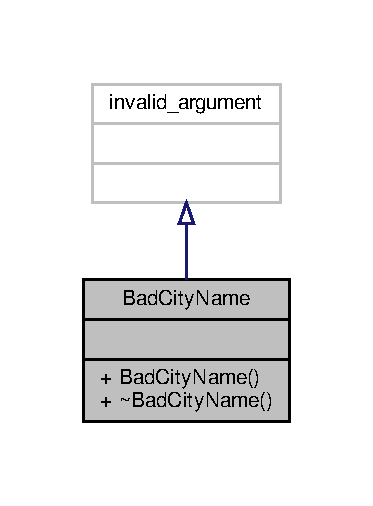
\includegraphics[width=179pt]{class_bad_city_name__inherit__graph}
\end{center}
\end{figure}
\subsection*{Public Member Functions}
\begin{DoxyCompactItemize}
\item 
\hyperlink{class_bad_city_name_a8e630c7dcfd5b617e93453fdb925146a}{Bad\+City\+Name} ()
\item 
virtual \hyperlink{class_bad_city_name_aaa7bda78c16c0f8ef6ebee0c68c03c29}{$\sim$\+Bad\+City\+Name} ()
\end{DoxyCompactItemize}


\subsection{Constructor \& Destructor Documentation}
\mbox{\Hypertarget{class_bad_city_name_a8e630c7dcfd5b617e93453fdb925146a}\label{class_bad_city_name_a8e630c7dcfd5b617e93453fdb925146a}} 
\index{Bad\+City\+Name@{Bad\+City\+Name}!Bad\+City\+Name@{Bad\+City\+Name}}
\index{Bad\+City\+Name@{Bad\+City\+Name}!Bad\+City\+Name@{Bad\+City\+Name}}
\subsubsection{\texorpdfstring{Bad\+City\+Name()}{BadCityName()}}
{\footnotesize\ttfamily Bad\+City\+Name\+::\+Bad\+City\+Name (\begin{DoxyParamCaption}{ }\end{DoxyParamCaption})\hspace{0.3cm}{\ttfamily [inline]}}

\mbox{\Hypertarget{class_bad_city_name_aaa7bda78c16c0f8ef6ebee0c68c03c29}\label{class_bad_city_name_aaa7bda78c16c0f8ef6ebee0c68c03c29}} 
\index{Bad\+City\+Name@{Bad\+City\+Name}!````~Bad\+City\+Name@{$\sim$\+Bad\+City\+Name}}
\index{````~Bad\+City\+Name@{$\sim$\+Bad\+City\+Name}!Bad\+City\+Name@{Bad\+City\+Name}}
\subsubsection{\texorpdfstring{$\sim$\+Bad\+City\+Name()}{~BadCityName()}}
{\footnotesize\ttfamily Bad\+City\+Name\+::$\sim$\+Bad\+City\+Name (\begin{DoxyParamCaption}{ }\end{DoxyParamCaption})\hspace{0.3cm}{\ttfamily [virtual]}}



The documentation for this class was generated from the following files\+:\begin{DoxyCompactItemize}
\item 
\hyperlink{hotels_8h}{hotels.\+h}\item 
\hyperlink{hotels_8cpp}{hotels.\+cpp}\end{DoxyCompactItemize}

\hypertarget{class_bad_file_name}{}\section{Bad\+File\+Name Class Reference}
\label{class_bad_file_name}\index{Bad\+File\+Name@{Bad\+File\+Name}}


{\ttfamily \#include $<$hotels.\+h$>$}



Inheritance diagram for Bad\+File\+Name\+:\nopagebreak
\begin{figure}[H]
\begin{center}
\leavevmode
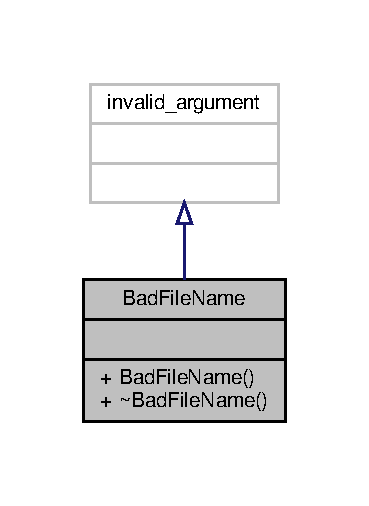
\includegraphics[width=177pt]{class_bad_file_name__inherit__graph}
\end{center}
\end{figure}
\subsection*{Public Member Functions}
\begin{DoxyCompactItemize}
\item 
\hyperlink{class_bad_file_name_adc47fdc3b0868830a1062fbc080fd735}{Bad\+File\+Name} ()
\item 
virtual \hyperlink{class_bad_file_name_a4ac0074ff0e544a3ffc6a18c8bdc1273}{$\sim$\+Bad\+File\+Name} ()
\end{DoxyCompactItemize}


\subsection{Constructor \& Destructor Documentation}
\mbox{\Hypertarget{class_bad_file_name_adc47fdc3b0868830a1062fbc080fd735}\label{class_bad_file_name_adc47fdc3b0868830a1062fbc080fd735}} 
\index{Bad\+File\+Name@{Bad\+File\+Name}!Bad\+File\+Name@{Bad\+File\+Name}}
\index{Bad\+File\+Name@{Bad\+File\+Name}!Bad\+File\+Name@{Bad\+File\+Name}}
\subsubsection{\texorpdfstring{Bad\+File\+Name()}{BadFileName()}}
{\footnotesize\ttfamily Bad\+File\+Name\+::\+Bad\+File\+Name (\begin{DoxyParamCaption}{ }\end{DoxyParamCaption})\hspace{0.3cm}{\ttfamily [inline]}}

Here is the call graph for this function\+:\nopagebreak
\begin{figure}[H]
\begin{center}
\leavevmode
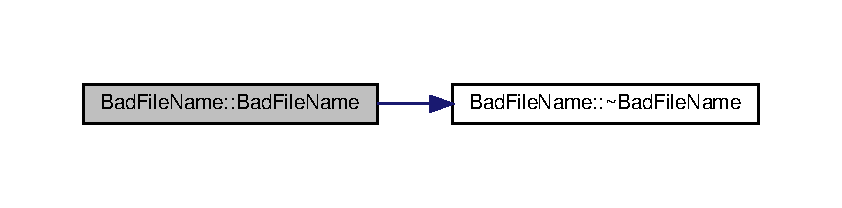
\includegraphics[width=350pt]{class_bad_file_name_adc47fdc3b0868830a1062fbc080fd735_cgraph}
\end{center}
\end{figure}
\mbox{\Hypertarget{class_bad_file_name_a4ac0074ff0e544a3ffc6a18c8bdc1273}\label{class_bad_file_name_a4ac0074ff0e544a3ffc6a18c8bdc1273}} 
\index{Bad\+File\+Name@{Bad\+File\+Name}!````~Bad\+File\+Name@{$\sim$\+Bad\+File\+Name}}
\index{````~Bad\+File\+Name@{$\sim$\+Bad\+File\+Name}!Bad\+File\+Name@{Bad\+File\+Name}}
\subsubsection{\texorpdfstring{$\sim$\+Bad\+File\+Name()}{~BadFileName()}}
{\footnotesize\ttfamily Bad\+File\+Name\+::$\sim$\+Bad\+File\+Name (\begin{DoxyParamCaption}{ }\end{DoxyParamCaption})\hspace{0.3cm}{\ttfamily [virtual]}}

Here is the caller graph for this function\+:\nopagebreak
\begin{figure}[H]
\begin{center}
\leavevmode
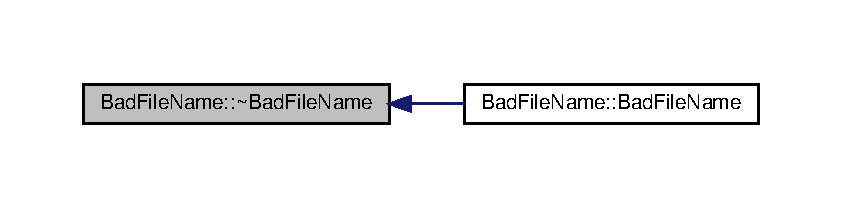
\includegraphics[width=350pt]{class_bad_file_name_a4ac0074ff0e544a3ffc6a18c8bdc1273_icgraph}
\end{center}
\end{figure}


The documentation for this class was generated from the following files\+:\begin{DoxyCompactItemize}
\item 
\hyperlink{hotels_8h}{hotels.\+h}\item 
\hyperlink{hotels_8cpp}{hotels.\+cpp}\end{DoxyCompactItemize}

\hypertarget{class_bad_hotel_name}{}\section{Bad\+Hotel\+Name Class Reference}
\label{class_bad_hotel_name}\index{Bad\+Hotel\+Name@{Bad\+Hotel\+Name}}


{\ttfamily \#include $<$hotels.\+h$>$}



Inheritance diagram for Bad\+Hotel\+Name\+:\nopagebreak
\begin{figure}[H]
\begin{center}
\leavevmode
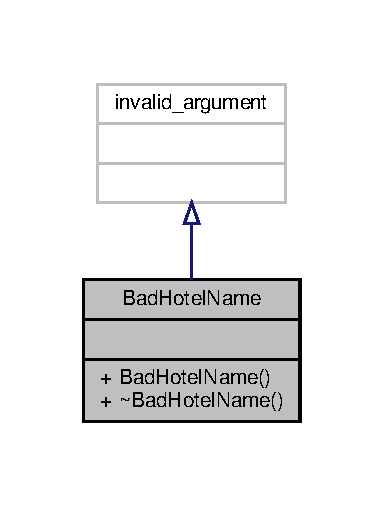
\includegraphics[width=184pt]{class_bad_hotel_name__inherit__graph}
\end{center}
\end{figure}
\subsection*{Public Member Functions}
\begin{DoxyCompactItemize}
\item 
\hyperlink{class_bad_hotel_name_a3e89385bf509245a838c1fcba3736a89}{Bad\+Hotel\+Name} ()
\item 
virtual \hyperlink{class_bad_hotel_name_aa2ad2390a5422aacbb9c61109957d58a}{$\sim$\+Bad\+Hotel\+Name} ()
\end{DoxyCompactItemize}


\subsection{Constructor \& Destructor Documentation}
\mbox{\Hypertarget{class_bad_hotel_name_a3e89385bf509245a838c1fcba3736a89}\label{class_bad_hotel_name_a3e89385bf509245a838c1fcba3736a89}} 
\index{Bad\+Hotel\+Name@{Bad\+Hotel\+Name}!Bad\+Hotel\+Name@{Bad\+Hotel\+Name}}
\index{Bad\+Hotel\+Name@{Bad\+Hotel\+Name}!Bad\+Hotel\+Name@{Bad\+Hotel\+Name}}
\subsubsection{\texorpdfstring{Bad\+Hotel\+Name()}{BadHotelName()}}
{\footnotesize\ttfamily Bad\+Hotel\+Name\+::\+Bad\+Hotel\+Name (\begin{DoxyParamCaption}{ }\end{DoxyParamCaption})\hspace{0.3cm}{\ttfamily [inline]}}

\mbox{\Hypertarget{class_bad_hotel_name_aa2ad2390a5422aacbb9c61109957d58a}\label{class_bad_hotel_name_aa2ad2390a5422aacbb9c61109957d58a}} 
\index{Bad\+Hotel\+Name@{Bad\+Hotel\+Name}!````~Bad\+Hotel\+Name@{$\sim$\+Bad\+Hotel\+Name}}
\index{````~Bad\+Hotel\+Name@{$\sim$\+Bad\+Hotel\+Name}!Bad\+Hotel\+Name@{Bad\+Hotel\+Name}}
\subsubsection{\texorpdfstring{$\sim$\+Bad\+Hotel\+Name()}{~BadHotelName()}}
{\footnotesize\ttfamily Bad\+Hotel\+Name\+::$\sim$\+Bad\+Hotel\+Name (\begin{DoxyParamCaption}{ }\end{DoxyParamCaption})\hspace{0.3cm}{\ttfamily [virtual]}}



The documentation for this class was generated from the following files\+:\begin{DoxyCompactItemize}
\item 
\hyperlink{hotels_8h}{hotels.\+h}\item 
\hyperlink{hotels_8cpp}{hotels.\+cpp}\end{DoxyCompactItemize}

\hypertarget{class_bad_room_number}{}\section{Bad\+Room\+Number Class Reference}
\label{class_bad_room_number}\index{Bad\+Room\+Number@{Bad\+Room\+Number}}


{\ttfamily \#include $<$hotels.\+h$>$}



Inheritance diagram for Bad\+Room\+Number\+:\nopagebreak
\begin{figure}[H]
\begin{center}
\leavevmode
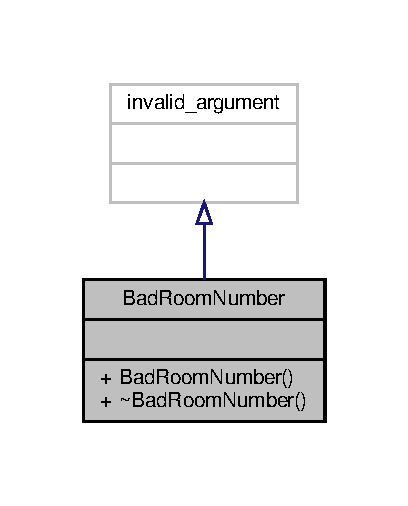
\includegraphics[width=196pt]{class_bad_room_number__inherit__graph}
\end{center}
\end{figure}
\subsection*{Public Member Functions}
\begin{DoxyCompactItemize}
\item 
\hyperlink{class_bad_room_number_a5bbd9fb21e5e6b8d29247b7714a478bd}{Bad\+Room\+Number} ()
\item 
virtual \hyperlink{class_bad_room_number_a3691fb5baacd1a49aa96fd6ed7256ef8}{$\sim$\+Bad\+Room\+Number} ()
\end{DoxyCompactItemize}


\subsection{Constructor \& Destructor Documentation}
\mbox{\Hypertarget{class_bad_room_number_a5bbd9fb21e5e6b8d29247b7714a478bd}\label{class_bad_room_number_a5bbd9fb21e5e6b8d29247b7714a478bd}} 
\index{Bad\+Room\+Number@{Bad\+Room\+Number}!Bad\+Room\+Number@{Bad\+Room\+Number}}
\index{Bad\+Room\+Number@{Bad\+Room\+Number}!Bad\+Room\+Number@{Bad\+Room\+Number}}
\subsubsection{\texorpdfstring{Bad\+Room\+Number()}{BadRoomNumber()}}
{\footnotesize\ttfamily Bad\+Room\+Number\+::\+Bad\+Room\+Number (\begin{DoxyParamCaption}{ }\end{DoxyParamCaption})\hspace{0.3cm}{\ttfamily [inline]}}

\mbox{\Hypertarget{class_bad_room_number_a3691fb5baacd1a49aa96fd6ed7256ef8}\label{class_bad_room_number_a3691fb5baacd1a49aa96fd6ed7256ef8}} 
\index{Bad\+Room\+Number@{Bad\+Room\+Number}!````~Bad\+Room\+Number@{$\sim$\+Bad\+Room\+Number}}
\index{````~Bad\+Room\+Number@{$\sim$\+Bad\+Room\+Number}!Bad\+Room\+Number@{Bad\+Room\+Number}}
\subsubsection{\texorpdfstring{$\sim$\+Bad\+Room\+Number()}{~BadRoomNumber()}}
{\footnotesize\ttfamily Bad\+Room\+Number\+::$\sim$\+Bad\+Room\+Number (\begin{DoxyParamCaption}{ }\end{DoxyParamCaption})\hspace{0.3cm}{\ttfamily [virtual]}}



The documentation for this class was generated from the following files\+:\begin{DoxyCompactItemize}
\item 
\hyperlink{hotels_8h}{hotels.\+h}\item 
\hyperlink{hotels_8cpp}{hotels.\+cpp}\end{DoxyCompactItemize}

\hypertarget{class_city}{}\section{City Class Reference}
\label{class_city}\index{City@{City}}


{\ttfamily \#include $<$hotels.\+h$>$}

\subsection*{Public Member Functions}
\begin{DoxyCompactItemize}
\item 
\hyperlink{class_city_ac0f0f98a4b34f6035ce375b249ea1f6f}{City} (string m\+\_\+name, ifstream \&in\+File, \hyperlink{class_data_base}{Data\+Base} $\ast$m\+\_\+parent)
\item 
\hyperlink{class_city_a32fffd38b77f72bf8ffdced4db06db41}{City} (string m\+\_\+name)
\item 
\hyperlink{class_city_ae95feee8a1d4e1f14ea41ec89b47304f}{$\sim$\+City} ()
\item 
\hyperlink{class_data_base}{Data\+Base} \& \hyperlink{class_city_a77c96bacad3ab36d48811749f7ae6c82}{get\+Parent} () const
\item 
vector$<$ \hyperlink{class_hotel}{Hotel} $\ast$ $>$ \hyperlink{class_city_adf8a1f3a0a67ecc07eb4eff1ee3c4e9b}{get\+Children} ()
\item 
void \hyperlink{class_city_af0fcf2e1e6da71f2b72444d9984d7163}{add\+Hotel} (\hyperlink{class_hotel}{Hotel} $\ast$htl)
\item 
\hyperlink{class_city_a41215eb7ca34723453b709bd20c0a1ae}{operator string} () const
\item 
\hyperlink{class_hotel}{Hotel} \& \hyperlink{class_city_a1215390b5e3b11dc19abeedcb096b720}{get\+Hotel} (string hotel\+Name) const
\item 
void \hyperlink{class_city_a18463913234ae61550b62693c7dd10a3}{show} (ostream \&os) const
\item 
void \hyperlink{class_city_ab8d15e9920d57b5892e073198dca0371}{show\+Reservations} (ostream \&os) const
\end{DoxyCompactItemize}


\subsection{Constructor \& Destructor Documentation}
\mbox{\Hypertarget{class_city_ac0f0f98a4b34f6035ce375b249ea1f6f}\label{class_city_ac0f0f98a4b34f6035ce375b249ea1f6f}} 
\index{City@{City}!City@{City}}
\index{City@{City}!City@{City}}
\subsubsection{\texorpdfstring{City()}{City()}\hspace{0.1cm}{\footnotesize\ttfamily [1/2]}}
{\footnotesize\ttfamily City\+::\+City (\begin{DoxyParamCaption}\item[{string}]{m\+\_\+name,  }\item[{ifstream \&}]{in\+File,  }\item[{\hyperlink{class_data_base}{Data\+Base} $\ast$}]{m\+\_\+parent }\end{DoxyParamCaption})}

Here is the call graph for this function\+:\nopagebreak
\begin{figure}[H]
\begin{center}
\leavevmode
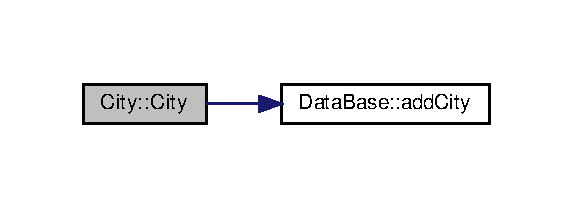
\includegraphics[width=275pt]{class_city_ac0f0f98a4b34f6035ce375b249ea1f6f_cgraph}
\end{center}
\end{figure}
\mbox{\Hypertarget{class_city_a32fffd38b77f72bf8ffdced4db06db41}\label{class_city_a32fffd38b77f72bf8ffdced4db06db41}} 
\index{City@{City}!City@{City}}
\index{City@{City}!City@{City}}
\subsubsection{\texorpdfstring{City()}{City()}\hspace{0.1cm}{\footnotesize\ttfamily [2/2]}}
{\footnotesize\ttfamily City\+::\+City (\begin{DoxyParamCaption}\item[{string}]{m\+\_\+name }\end{DoxyParamCaption})\hspace{0.3cm}{\ttfamily [inline]}}

\mbox{\Hypertarget{class_city_ae95feee8a1d4e1f14ea41ec89b47304f}\label{class_city_ae95feee8a1d4e1f14ea41ec89b47304f}} 
\index{City@{City}!````~City@{$\sim$\+City}}
\index{````~City@{$\sim$\+City}!City@{City}}
\subsubsection{\texorpdfstring{$\sim$\+City()}{~City()}}
{\footnotesize\ttfamily City\+::$\sim$\+City (\begin{DoxyParamCaption}{ }\end{DoxyParamCaption})\hspace{0.3cm}{\ttfamily [inline]}}



\subsection{Member Function Documentation}
\mbox{\Hypertarget{class_city_af0fcf2e1e6da71f2b72444d9984d7163}\label{class_city_af0fcf2e1e6da71f2b72444d9984d7163}} 
\index{City@{City}!add\+Hotel@{add\+Hotel}}
\index{add\+Hotel@{add\+Hotel}!City@{City}}
\subsubsection{\texorpdfstring{add\+Hotel()}{addHotel()}}
{\footnotesize\ttfamily void City\+::add\+Hotel (\begin{DoxyParamCaption}\item[{\hyperlink{class_hotel}{Hotel} $\ast$}]{htl }\end{DoxyParamCaption})\hspace{0.3cm}{\ttfamily [inline]}}

Here is the caller graph for this function\+:\nopagebreak
\begin{figure}[H]
\begin{center}
\leavevmode
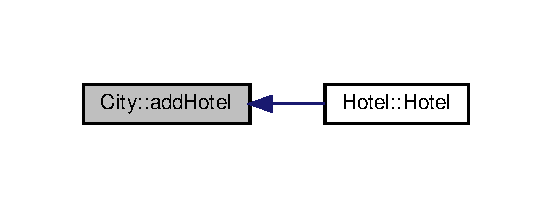
\includegraphics[width=265pt]{class_city_af0fcf2e1e6da71f2b72444d9984d7163_icgraph}
\end{center}
\end{figure}
\mbox{\Hypertarget{class_city_adf8a1f3a0a67ecc07eb4eff1ee3c4e9b}\label{class_city_adf8a1f3a0a67ecc07eb4eff1ee3c4e9b}} 
\index{City@{City}!get\+Children@{get\+Children}}
\index{get\+Children@{get\+Children}!City@{City}}
\subsubsection{\texorpdfstring{get\+Children()}{getChildren()}}
{\footnotesize\ttfamily vector$<$\hyperlink{class_hotel}{Hotel} $\ast$$>$ City\+::get\+Children (\begin{DoxyParamCaption}{ }\end{DoxyParamCaption})\hspace{0.3cm}{\ttfamily [inline]}}

\mbox{\Hypertarget{class_city_a1215390b5e3b11dc19abeedcb096b720}\label{class_city_a1215390b5e3b11dc19abeedcb096b720}} 
\index{City@{City}!get\+Hotel@{get\+Hotel}}
\index{get\+Hotel@{get\+Hotel}!City@{City}}
\subsubsection{\texorpdfstring{get\+Hotel()}{getHotel()}}
{\footnotesize\ttfamily \hyperlink{class_hotel}{Hotel} \& City\+::get\+Hotel (\begin{DoxyParamCaption}\item[{string}]{hotel\+Name }\end{DoxyParamCaption}) const}

Here is the call graph for this function\+:\nopagebreak
\begin{figure}[H]
\begin{center}
\leavevmode
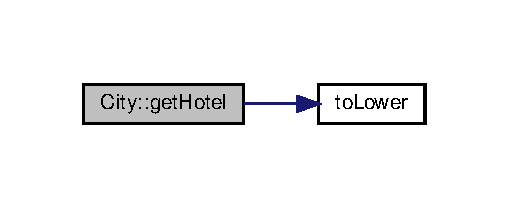
\includegraphics[width=244pt]{class_city_a1215390b5e3b11dc19abeedcb096b720_cgraph}
\end{center}
\end{figure}
Here is the caller graph for this function\+:\nopagebreak
\begin{figure}[H]
\begin{center}
\leavevmode
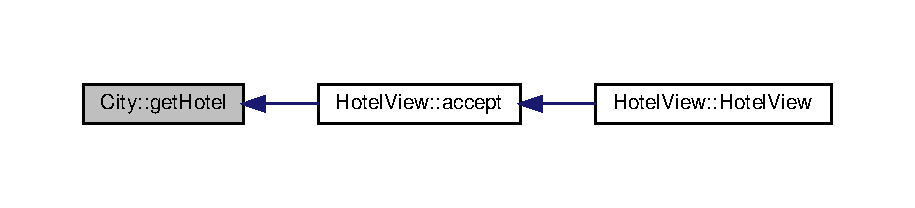
\includegraphics[width=350pt]{class_city_a1215390b5e3b11dc19abeedcb096b720_icgraph}
\end{center}
\end{figure}
\mbox{\Hypertarget{class_city_a77c96bacad3ab36d48811749f7ae6c82}\label{class_city_a77c96bacad3ab36d48811749f7ae6c82}} 
\index{City@{City}!get\+Parent@{get\+Parent}}
\index{get\+Parent@{get\+Parent}!City@{City}}
\subsubsection{\texorpdfstring{get\+Parent()}{getParent()}}
{\footnotesize\ttfamily \hyperlink{class_data_base}{Data\+Base}\& City\+::get\+Parent (\begin{DoxyParamCaption}{ }\end{DoxyParamCaption}) const\hspace{0.3cm}{\ttfamily [inline]}}

\mbox{\Hypertarget{class_city_a41215eb7ca34723453b709bd20c0a1ae}\label{class_city_a41215eb7ca34723453b709bd20c0a1ae}} 
\index{City@{City}!operator string@{operator string}}
\index{operator string@{operator string}!City@{City}}
\subsubsection{\texorpdfstring{operator string()}{operator string()}}
{\footnotesize\ttfamily City\+::operator string (\begin{DoxyParamCaption}{ }\end{DoxyParamCaption}) const\hspace{0.3cm}{\ttfamily [inline]}, {\ttfamily [explicit]}}

\mbox{\Hypertarget{class_city_a18463913234ae61550b62693c7dd10a3}\label{class_city_a18463913234ae61550b62693c7dd10a3}} 
\index{City@{City}!show@{show}}
\index{show@{show}!City@{City}}
\subsubsection{\texorpdfstring{show()}{show()}}
{\footnotesize\ttfamily void City\+::show (\begin{DoxyParamCaption}\item[{ostream \&}]{os }\end{DoxyParamCaption}) const}

\mbox{\Hypertarget{class_city_ab8d15e9920d57b5892e073198dca0371}\label{class_city_ab8d15e9920d57b5892e073198dca0371}} 
\index{City@{City}!show\+Reservations@{show\+Reservations}}
\index{show\+Reservations@{show\+Reservations}!City@{City}}
\subsubsection{\texorpdfstring{show\+Reservations()}{showReservations()}}
{\footnotesize\ttfamily void City\+::show\+Reservations (\begin{DoxyParamCaption}\item[{ostream \&}]{os }\end{DoxyParamCaption}) const}



The documentation for this class was generated from the following files\+:\begin{DoxyCompactItemize}
\item 
\hyperlink{hotels_8h}{hotels.\+h}\item 
\hyperlink{hotels_8cpp}{hotels.\+cpp}\end{DoxyCompactItemize}

\hypertarget{class_data_base}{}\section{Data\+Base Class Reference}
\label{class_data_base}\index{Data\+Base@{Data\+Base}}


{\ttfamily \#include $<$hotels.\+h$>$}

\subsection*{Public Member Functions}
\begin{DoxyCompactItemize}
\item 
\hyperlink{class_data_base_ac9231375bb821d55201b26f9049c8661}{Data\+Base} (string file\+Name)
\item 
\hyperlink{class_data_base_a9d4629e705ccaa4897e9650222a2a648}{$\sim$\+Data\+Base} ()
\item 
void \hyperlink{class_data_base_a090b459850b95afaaa23cba4339508e3}{add\+City} (\hyperlink{class_city}{City} $\ast$cty)
\item 
vector$<$ \hyperlink{class_city}{City} $\ast$ $>$ \hyperlink{class_data_base_af0444cd53bc289472c9e2f09a83afaf4}{get\+Children} ()
\item 
\hyperlink{class_city}{City} \& \hyperlink{class_data_base_acf702c18049dec5367c04249c8b431f7}{get\+City} (string m\+\_\+city) const
\item 
vector$<$ \hyperlink{class_hotel}{Hotel} $\ast$ $>$ \hyperlink{class_data_base_a0a4e75be22c35f5da860ce89cf264018}{get\+Hotels} (string m\+\_\+city)
\item 
void \hyperlink{class_data_base_a47afe882e3b264b43e8cb4bf3f894a68}{show} (ostream \&os) const
\item 
void \hyperlink{class_data_base_a8ea4492457e052838b3b9d41c00d786d}{show\+Reservations} (ostream \&os) const
\item 
void \hyperlink{class_data_base_ae099589c13d77b31a311fc0469250288}{write\+To\+File} ()
\item 
vector$<$ string $>$ \hyperlink{class_data_base_a8e5b464d772e7cdac7c10b5548fef1b2}{get\+Reservations} (string sur\+Name\+Name)
\end{DoxyCompactItemize}


\subsection{Constructor \& Destructor Documentation}
\mbox{\Hypertarget{class_data_base_ac9231375bb821d55201b26f9049c8661}\label{class_data_base_ac9231375bb821d55201b26f9049c8661}} 
\index{Data\+Base@{Data\+Base}!Data\+Base@{Data\+Base}}
\index{Data\+Base@{Data\+Base}!Data\+Base@{Data\+Base}}
\subsubsection{\texorpdfstring{Data\+Base()}{DataBase()}}
{\footnotesize\ttfamily Data\+Base\+::\+Data\+Base (\begin{DoxyParamCaption}\item[{string}]{file\+Name }\end{DoxyParamCaption})}

\mbox{\Hypertarget{class_data_base_a9d4629e705ccaa4897e9650222a2a648}\label{class_data_base_a9d4629e705ccaa4897e9650222a2a648}} 
\index{Data\+Base@{Data\+Base}!````~Data\+Base@{$\sim$\+Data\+Base}}
\index{````~Data\+Base@{$\sim$\+Data\+Base}!Data\+Base@{Data\+Base}}
\subsubsection{\texorpdfstring{$\sim$\+Data\+Base()}{~DataBase()}}
{\footnotesize\ttfamily Data\+Base\+::$\sim$\+Data\+Base (\begin{DoxyParamCaption}{ }\end{DoxyParamCaption})\hspace{0.3cm}{\ttfamily [inline]}}



\subsection{Member Function Documentation}
\mbox{\Hypertarget{class_data_base_a090b459850b95afaaa23cba4339508e3}\label{class_data_base_a090b459850b95afaaa23cba4339508e3}} 
\index{Data\+Base@{Data\+Base}!add\+City@{add\+City}}
\index{add\+City@{add\+City}!Data\+Base@{Data\+Base}}
\subsubsection{\texorpdfstring{add\+City()}{addCity()}}
{\footnotesize\ttfamily void Data\+Base\+::add\+City (\begin{DoxyParamCaption}\item[{\hyperlink{class_city}{City} $\ast$}]{cty }\end{DoxyParamCaption})\hspace{0.3cm}{\ttfamily [inline]}}

Here is the caller graph for this function\+:\nopagebreak
\begin{figure}[H]
\begin{center}
\leavevmode
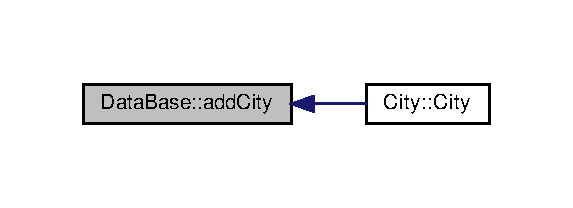
\includegraphics[width=275pt]{class_data_base_a090b459850b95afaaa23cba4339508e3_icgraph}
\end{center}
\end{figure}
\mbox{\Hypertarget{class_data_base_af0444cd53bc289472c9e2f09a83afaf4}\label{class_data_base_af0444cd53bc289472c9e2f09a83afaf4}} 
\index{Data\+Base@{Data\+Base}!get\+Children@{get\+Children}}
\index{get\+Children@{get\+Children}!Data\+Base@{Data\+Base}}
\subsubsection{\texorpdfstring{get\+Children()}{getChildren()}}
{\footnotesize\ttfamily vector$<$\hyperlink{class_city}{City} $\ast$$>$ Data\+Base\+::get\+Children (\begin{DoxyParamCaption}{ }\end{DoxyParamCaption})\hspace{0.3cm}{\ttfamily [inline]}}

Here is the caller graph for this function\+:\nopagebreak
\begin{figure}[H]
\begin{center}
\leavevmode
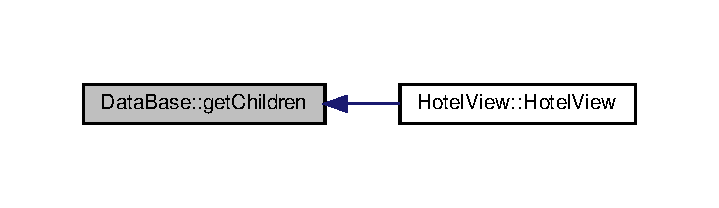
\includegraphics[width=345pt]{class_data_base_af0444cd53bc289472c9e2f09a83afaf4_icgraph}
\end{center}
\end{figure}
\mbox{\Hypertarget{class_data_base_acf702c18049dec5367c04249c8b431f7}\label{class_data_base_acf702c18049dec5367c04249c8b431f7}} 
\index{Data\+Base@{Data\+Base}!get\+City@{get\+City}}
\index{get\+City@{get\+City}!Data\+Base@{Data\+Base}}
\subsubsection{\texorpdfstring{get\+City()}{getCity()}}
{\footnotesize\ttfamily \hyperlink{class_city}{City}\& Data\+Base\+::get\+City (\begin{DoxyParamCaption}\item[{string}]{m\+\_\+city }\end{DoxyParamCaption}) const\hspace{0.3cm}{\ttfamily [inline]}}

Here is the call graph for this function\+:\nopagebreak
\begin{figure}[H]
\begin{center}
\leavevmode
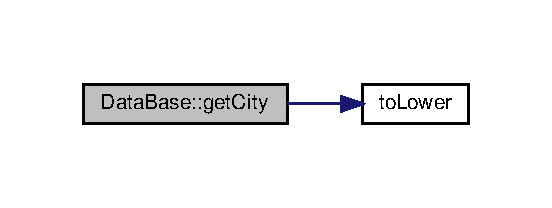
\includegraphics[width=265pt]{class_data_base_acf702c18049dec5367c04249c8b431f7_cgraph}
\end{center}
\end{figure}
Here is the caller graph for this function\+:\nopagebreak
\begin{figure}[H]
\begin{center}
\leavevmode
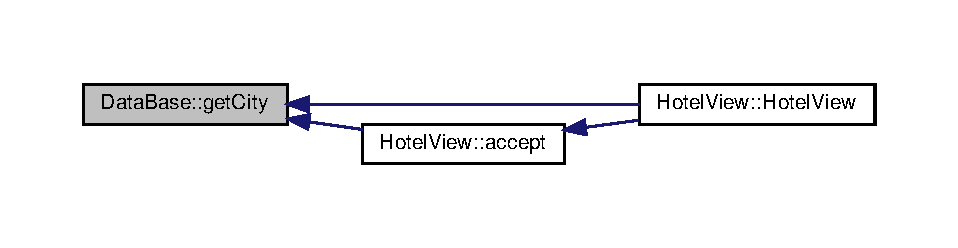
\includegraphics[width=350pt]{class_data_base_acf702c18049dec5367c04249c8b431f7_icgraph}
\end{center}
\end{figure}
\mbox{\Hypertarget{class_data_base_a0a4e75be22c35f5da860ce89cf264018}\label{class_data_base_a0a4e75be22c35f5da860ce89cf264018}} 
\index{Data\+Base@{Data\+Base}!get\+Hotels@{get\+Hotels}}
\index{get\+Hotels@{get\+Hotels}!Data\+Base@{Data\+Base}}
\subsubsection{\texorpdfstring{get\+Hotels()}{getHotels()}}
{\footnotesize\ttfamily vector$<$\hyperlink{class_hotel}{Hotel}$\ast$$>$ Data\+Base\+::get\+Hotels (\begin{DoxyParamCaption}\item[{string}]{m\+\_\+city }\end{DoxyParamCaption})\hspace{0.3cm}{\ttfamily [inline]}}

Here is the caller graph for this function\+:\nopagebreak
\begin{figure}[H]
\begin{center}
\leavevmode
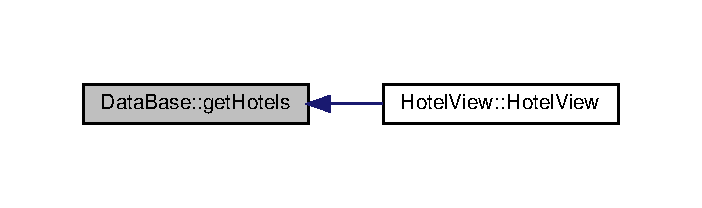
\includegraphics[width=337pt]{class_data_base_a0a4e75be22c35f5da860ce89cf264018_icgraph}
\end{center}
\end{figure}
\mbox{\Hypertarget{class_data_base_a8e5b464d772e7cdac7c10b5548fef1b2}\label{class_data_base_a8e5b464d772e7cdac7c10b5548fef1b2}} 
\index{Data\+Base@{Data\+Base}!get\+Reservations@{get\+Reservations}}
\index{get\+Reservations@{get\+Reservations}!Data\+Base@{Data\+Base}}
\subsubsection{\texorpdfstring{get\+Reservations()}{getReservations()}}
{\footnotesize\ttfamily vector$<$string$>$ Data\+Base\+::get\+Reservations (\begin{DoxyParamCaption}\item[{string}]{sur\+Name\+Name }\end{DoxyParamCaption})\hspace{0.3cm}{\ttfamily [inline]}}

Here is the caller graph for this function\+:\nopagebreak
\begin{figure}[H]
\begin{center}
\leavevmode
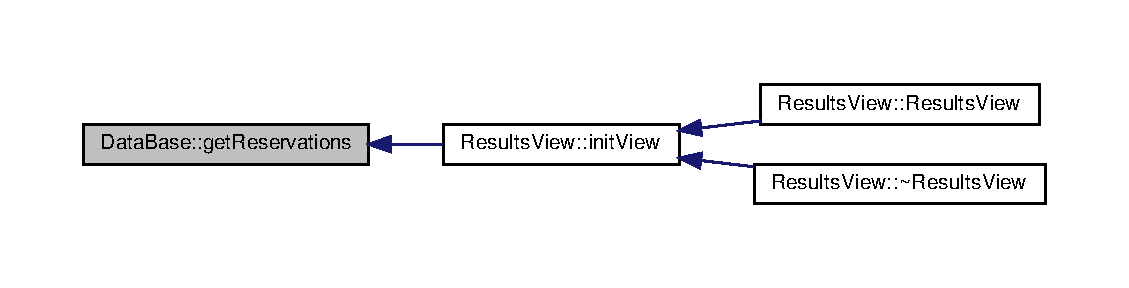
\includegraphics[width=350pt]{class_data_base_a8e5b464d772e7cdac7c10b5548fef1b2_icgraph}
\end{center}
\end{figure}
\mbox{\Hypertarget{class_data_base_a47afe882e3b264b43e8cb4bf3f894a68}\label{class_data_base_a47afe882e3b264b43e8cb4bf3f894a68}} 
\index{Data\+Base@{Data\+Base}!show@{show}}
\index{show@{show}!Data\+Base@{Data\+Base}}
\subsubsection{\texorpdfstring{show()}{show()}}
{\footnotesize\ttfamily void Data\+Base\+::show (\begin{DoxyParamCaption}\item[{ostream \&}]{os }\end{DoxyParamCaption}) const\hspace{0.3cm}{\ttfamily [inline]}}

\mbox{\Hypertarget{class_data_base_a8ea4492457e052838b3b9d41c00d786d}\label{class_data_base_a8ea4492457e052838b3b9d41c00d786d}} 
\index{Data\+Base@{Data\+Base}!show\+Reservations@{show\+Reservations}}
\index{show\+Reservations@{show\+Reservations}!Data\+Base@{Data\+Base}}
\subsubsection{\texorpdfstring{show\+Reservations()}{showReservations()}}
{\footnotesize\ttfamily void Data\+Base\+::show\+Reservations (\begin{DoxyParamCaption}\item[{ostream \&}]{os }\end{DoxyParamCaption}) const\hspace{0.3cm}{\ttfamily [inline]}}

\mbox{\Hypertarget{class_data_base_ae099589c13d77b31a311fc0469250288}\label{class_data_base_ae099589c13d77b31a311fc0469250288}} 
\index{Data\+Base@{Data\+Base}!write\+To\+File@{write\+To\+File}}
\index{write\+To\+File@{write\+To\+File}!Data\+Base@{Data\+Base}}
\subsubsection{\texorpdfstring{write\+To\+File()}{writeToFile()}}
{\footnotesize\ttfamily void Data\+Base\+::write\+To\+File (\begin{DoxyParamCaption}{ }\end{DoxyParamCaption})\hspace{0.3cm}{\ttfamily [inline]}}



The documentation for this class was generated from the following files\+:\begin{DoxyCompactItemize}
\item 
\hyperlink{hotels_8h}{hotels.\+h}\item 
\hyperlink{hotels_8cpp}{hotels.\+cpp}\end{DoxyCompactItemize}

\hypertarget{class_hotel}{}\section{Hotel Class Reference}
\label{class_hotel}\index{Hotel@{Hotel}}


{\ttfamily \#include $<$hotels.\+h$>$}

\subsection*{Public Member Functions}
\begin{DoxyCompactItemize}
\item 
\hyperlink{class_hotel_aa74ecd8c4a1b959628d28779efb00c46}{Hotel} (string m\+\_\+name, int m\+\_\+price\+For\+Night, \hyperlink{class_city}{City} $\ast$m\+\_\+parent)
\item 
\hyperlink{class_hotel_ae4c9782535c021bc10c028339dc29310}{$\sim$\+Hotel} ()
\item 
void \hyperlink{class_hotel_a81dd1c4ed4589770fad50517688035a1}{add\+Room} (\hyperlink{class_room}{Room} $\ast$rom)
\item 
\hyperlink{class_hotel_a8528cf910b707df791daed38519c895e}{operator string} ()
\item 
double \hyperlink{class_hotel_a0c9a17ff69bb3ecec9e8938b8532defa}{get\+Price} () const
\item 
vector$<$ \hyperlink{class_room}{Room} $\ast$ $>$ \hyperlink{class_hotel_a1e22ca2270cf28ea4b03497701d970a1}{get\+Children} ()
\item 
const \hyperlink{class_city}{City} \& \hyperlink{class_hotel_a10b09b0e1309de50bc7cc6ebafb822af}{get\+Parent} () const
\item 
bool \hyperlink{class_hotel_aa11ad566c8765362795e53f4088e10d7}{is\+Free} (Q\+Date m\+\_\+first\+Day, Q\+Date m\+\_\+last\+Day) const
\item 
\hyperlink{class_room}{Room} \& \hyperlink{class_hotel_ac836a89654a7561169ca1523f0365861}{get\+Room} (Q\+Date first\+Day, Q\+Date last\+Day) const
\item 
\hyperlink{class_room}{Room} \& \hyperlink{class_hotel_a5188fb61eb6bd1fa3e971f2457c50947}{get\+Room} (int m\+\_\+number) const
\item 
void \hyperlink{class_hotel_a78710e2a296cf886845a7fe39b9b9ddb}{show} (ostream \&os) const
\item 
bool \hyperlink{class_hotel_a05e576bdd914079ceb0781323408014b}{has\+Reservations} () const
\item 
void \hyperlink{class_hotel_abbae1165abd672d1568cd3dcec64000e}{show\+Reservations} (ostream \&os) const
\end{DoxyCompactItemize}


\subsection{Constructor \& Destructor Documentation}
\mbox{\Hypertarget{class_hotel_aa74ecd8c4a1b959628d28779efb00c46}\label{class_hotel_aa74ecd8c4a1b959628d28779efb00c46}} 
\index{Hotel@{Hotel}!Hotel@{Hotel}}
\index{Hotel@{Hotel}!Hotel@{Hotel}}
\subsubsection{\texorpdfstring{Hotel()}{Hotel()}}
{\footnotesize\ttfamily Hotel\+::\+Hotel (\begin{DoxyParamCaption}\item[{string}]{m\+\_\+name,  }\item[{int}]{m\+\_\+price\+For\+Night,  }\item[{\hyperlink{class_city}{City} $\ast$}]{m\+\_\+parent }\end{DoxyParamCaption})}

Here is the call graph for this function\+:\nopagebreak
\begin{figure}[H]
\begin{center}
\leavevmode
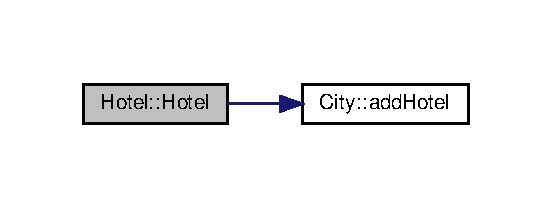
\includegraphics[width=265pt]{class_hotel_aa74ecd8c4a1b959628d28779efb00c46_cgraph}
\end{center}
\end{figure}
\mbox{\Hypertarget{class_hotel_ae4c9782535c021bc10c028339dc29310}\label{class_hotel_ae4c9782535c021bc10c028339dc29310}} 
\index{Hotel@{Hotel}!````~Hotel@{$\sim$\+Hotel}}
\index{````~Hotel@{$\sim$\+Hotel}!Hotel@{Hotel}}
\subsubsection{\texorpdfstring{$\sim$\+Hotel()}{~Hotel()}}
{\footnotesize\ttfamily Hotel\+::$\sim$\+Hotel (\begin{DoxyParamCaption}{ }\end{DoxyParamCaption})\hspace{0.3cm}{\ttfamily [inline]}}



\subsection{Member Function Documentation}
\mbox{\Hypertarget{class_hotel_a81dd1c4ed4589770fad50517688035a1}\label{class_hotel_a81dd1c4ed4589770fad50517688035a1}} 
\index{Hotel@{Hotel}!add\+Room@{add\+Room}}
\index{add\+Room@{add\+Room}!Hotel@{Hotel}}
\subsubsection{\texorpdfstring{add\+Room()}{addRoom()}}
{\footnotesize\ttfamily void Hotel\+::add\+Room (\begin{DoxyParamCaption}\item[{\hyperlink{class_room}{Room} $\ast$}]{rom }\end{DoxyParamCaption})\hspace{0.3cm}{\ttfamily [inline]}}

Here is the caller graph for this function\+:\nopagebreak
\begin{figure}[H]
\begin{center}
\leavevmode
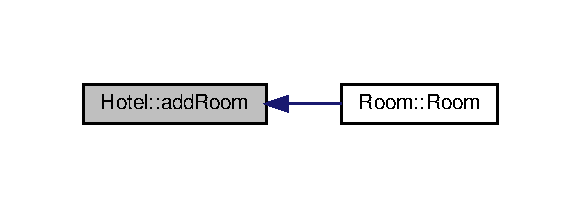
\includegraphics[width=279pt]{class_hotel_a81dd1c4ed4589770fad50517688035a1_icgraph}
\end{center}
\end{figure}
\mbox{\Hypertarget{class_hotel_a1e22ca2270cf28ea4b03497701d970a1}\label{class_hotel_a1e22ca2270cf28ea4b03497701d970a1}} 
\index{Hotel@{Hotel}!get\+Children@{get\+Children}}
\index{get\+Children@{get\+Children}!Hotel@{Hotel}}
\subsubsection{\texorpdfstring{get\+Children()}{getChildren()}}
{\footnotesize\ttfamily vector$<$\hyperlink{class_room}{Room} $\ast$$>$ Hotel\+::get\+Children (\begin{DoxyParamCaption}{ }\end{DoxyParamCaption})\hspace{0.3cm}{\ttfamily [inline]}}

\mbox{\Hypertarget{class_hotel_a10b09b0e1309de50bc7cc6ebafb822af}\label{class_hotel_a10b09b0e1309de50bc7cc6ebafb822af}} 
\index{Hotel@{Hotel}!get\+Parent@{get\+Parent}}
\index{get\+Parent@{get\+Parent}!Hotel@{Hotel}}
\subsubsection{\texorpdfstring{get\+Parent()}{getParent()}}
{\footnotesize\ttfamily const \hyperlink{class_city}{City}\& Hotel\+::get\+Parent (\begin{DoxyParamCaption}{ }\end{DoxyParamCaption}) const\hspace{0.3cm}{\ttfamily [inline]}}

Here is the caller graph for this function\+:\nopagebreak
\begin{figure}[H]
\begin{center}
\leavevmode
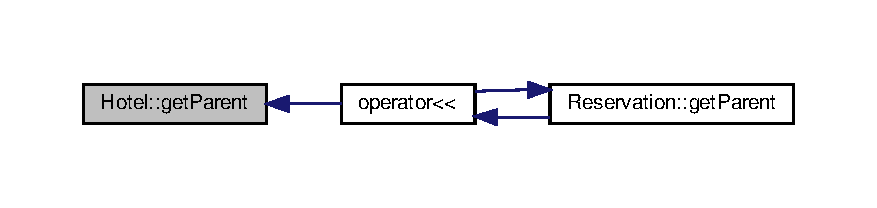
\includegraphics[width=350pt]{class_hotel_a10b09b0e1309de50bc7cc6ebafb822af_icgraph}
\end{center}
\end{figure}
\mbox{\Hypertarget{class_hotel_a0c9a17ff69bb3ecec9e8938b8532defa}\label{class_hotel_a0c9a17ff69bb3ecec9e8938b8532defa}} 
\index{Hotel@{Hotel}!get\+Price@{get\+Price}}
\index{get\+Price@{get\+Price}!Hotel@{Hotel}}
\subsubsection{\texorpdfstring{get\+Price()}{getPrice()}}
{\footnotesize\ttfamily double Hotel\+::get\+Price (\begin{DoxyParamCaption}{ }\end{DoxyParamCaption}) const\hspace{0.3cm}{\ttfamily [inline]}}

\mbox{\Hypertarget{class_hotel_ac836a89654a7561169ca1523f0365861}\label{class_hotel_ac836a89654a7561169ca1523f0365861}} 
\index{Hotel@{Hotel}!get\+Room@{get\+Room}}
\index{get\+Room@{get\+Room}!Hotel@{Hotel}}
\subsubsection{\texorpdfstring{get\+Room()}{getRoom()}\hspace{0.1cm}{\footnotesize\ttfamily [1/2]}}
{\footnotesize\ttfamily \hyperlink{class_room}{Room} \& Hotel\+::get\+Room (\begin{DoxyParamCaption}\item[{Q\+Date}]{first\+Day,  }\item[{Q\+Date}]{last\+Day }\end{DoxyParamCaption}) const}

Here is the caller graph for this function\+:\nopagebreak
\begin{figure}[H]
\begin{center}
\leavevmode
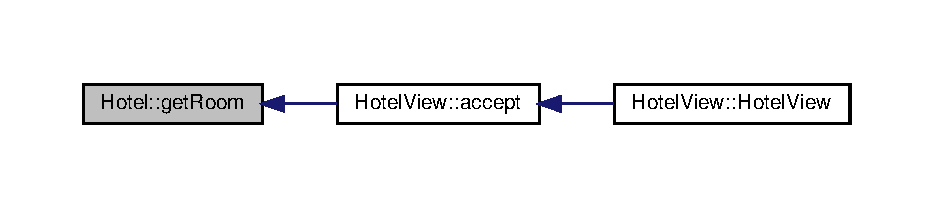
\includegraphics[width=350pt]{class_hotel_ac836a89654a7561169ca1523f0365861_icgraph}
\end{center}
\end{figure}
\mbox{\Hypertarget{class_hotel_a5188fb61eb6bd1fa3e971f2457c50947}\label{class_hotel_a5188fb61eb6bd1fa3e971f2457c50947}} 
\index{Hotel@{Hotel}!get\+Room@{get\+Room}}
\index{get\+Room@{get\+Room}!Hotel@{Hotel}}
\subsubsection{\texorpdfstring{get\+Room()}{getRoom()}\hspace{0.1cm}{\footnotesize\ttfamily [2/2]}}
{\footnotesize\ttfamily \hyperlink{class_room}{Room} \& Hotel\+::get\+Room (\begin{DoxyParamCaption}\item[{int}]{m\+\_\+number }\end{DoxyParamCaption}) const}

\mbox{\Hypertarget{class_hotel_a05e576bdd914079ceb0781323408014b}\label{class_hotel_a05e576bdd914079ceb0781323408014b}} 
\index{Hotel@{Hotel}!has\+Reservations@{has\+Reservations}}
\index{has\+Reservations@{has\+Reservations}!Hotel@{Hotel}}
\subsubsection{\texorpdfstring{has\+Reservations()}{hasReservations()}}
{\footnotesize\ttfamily bool Hotel\+::has\+Reservations (\begin{DoxyParamCaption}{ }\end{DoxyParamCaption}) const\hspace{0.3cm}{\ttfamily [inline]}}

\mbox{\Hypertarget{class_hotel_aa11ad566c8765362795e53f4088e10d7}\label{class_hotel_aa11ad566c8765362795e53f4088e10d7}} 
\index{Hotel@{Hotel}!is\+Free@{is\+Free}}
\index{is\+Free@{is\+Free}!Hotel@{Hotel}}
\subsubsection{\texorpdfstring{is\+Free()}{isFree()}}
{\footnotesize\ttfamily bool Hotel\+::is\+Free (\begin{DoxyParamCaption}\item[{Q\+Date}]{m\+\_\+first\+Day,  }\item[{Q\+Date}]{m\+\_\+last\+Day }\end{DoxyParamCaption}) const\hspace{0.3cm}{\ttfamily [inline]}}

\mbox{\Hypertarget{class_hotel_a8528cf910b707df791daed38519c895e}\label{class_hotel_a8528cf910b707df791daed38519c895e}} 
\index{Hotel@{Hotel}!operator string@{operator string}}
\index{operator string@{operator string}!Hotel@{Hotel}}
\subsubsection{\texorpdfstring{operator string()}{operator string()}}
{\footnotesize\ttfamily Hotel\+::operator string (\begin{DoxyParamCaption}{ }\end{DoxyParamCaption})\hspace{0.3cm}{\ttfamily [inline]}, {\ttfamily [explicit]}}

\mbox{\Hypertarget{class_hotel_a78710e2a296cf886845a7fe39b9b9ddb}\label{class_hotel_a78710e2a296cf886845a7fe39b9b9ddb}} 
\index{Hotel@{Hotel}!show@{show}}
\index{show@{show}!Hotel@{Hotel}}
\subsubsection{\texorpdfstring{show()}{show()}}
{\footnotesize\ttfamily void Hotel\+::show (\begin{DoxyParamCaption}\item[{ostream \&}]{os }\end{DoxyParamCaption}) const}

\mbox{\Hypertarget{class_hotel_abbae1165abd672d1568cd3dcec64000e}\label{class_hotel_abbae1165abd672d1568cd3dcec64000e}} 
\index{Hotel@{Hotel}!show\+Reservations@{show\+Reservations}}
\index{show\+Reservations@{show\+Reservations}!Hotel@{Hotel}}
\subsubsection{\texorpdfstring{show\+Reservations()}{showReservations()}}
{\footnotesize\ttfamily void Hotel\+::show\+Reservations (\begin{DoxyParamCaption}\item[{ostream \&}]{os }\end{DoxyParamCaption}) const}



The documentation for this class was generated from the following files\+:\begin{DoxyCompactItemize}
\item 
\hyperlink{hotels_8h}{hotels.\+h}\item 
\hyperlink{hotels_8cpp}{hotels.\+cpp}\end{DoxyCompactItemize}

\hypertarget{class_hotel_view}{}\section{Hotel\+View Class Reference}
\label{class_hotel_view}\index{Hotel\+View@{Hotel\+View}}


{\ttfamily \#include $<$hotelview.\+h$>$}



Inheritance diagram for Hotel\+View\+:\nopagebreak
\begin{figure}[H]
\begin{center}
\leavevmode
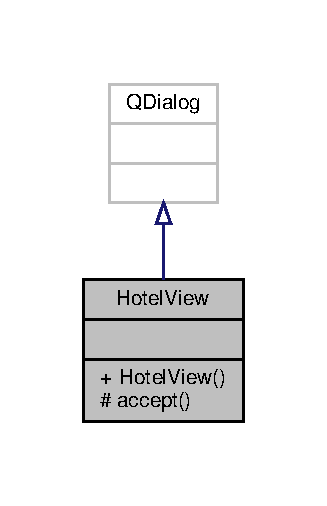
\includegraphics[width=157pt]{class_hotel_view__inherit__graph}
\end{center}
\end{figure}
\subsection*{Public Member Functions}
\begin{DoxyCompactItemize}
\item 
\hyperlink{class_hotel_view_adba641d84e83365cd5fc499666640dba}{Hotel\+View} (Q\+Widget $\ast$parent=nullptr)
\end{DoxyCompactItemize}
\subsection*{Protected Slots}
\begin{DoxyCompactItemize}
\item 
void \hyperlink{class_hotel_view_a88805d7379290f2540206d384ef962a1}{accept} ()
\end{DoxyCompactItemize}


\subsection{Constructor \& Destructor Documentation}
\mbox{\Hypertarget{class_hotel_view_adba641d84e83365cd5fc499666640dba}\label{class_hotel_view_adba641d84e83365cd5fc499666640dba}} 
\index{Hotel\+View@{Hotel\+View}!Hotel\+View@{Hotel\+View}}
\index{Hotel\+View@{Hotel\+View}!Hotel\+View@{Hotel\+View}}
\subsubsection{\texorpdfstring{Hotel\+View()}{HotelView()}}
{\footnotesize\ttfamily Hotel\+View\+::\+Hotel\+View (\begin{DoxyParamCaption}\item[{Q\+Widget $\ast$}]{parent = {\ttfamily nullptr} }\end{DoxyParamCaption})\hspace{0.3cm}{\ttfamily [explicit]}}

Here is the call graph for this function\+:\nopagebreak
\begin{figure}[H]
\begin{center}
\leavevmode
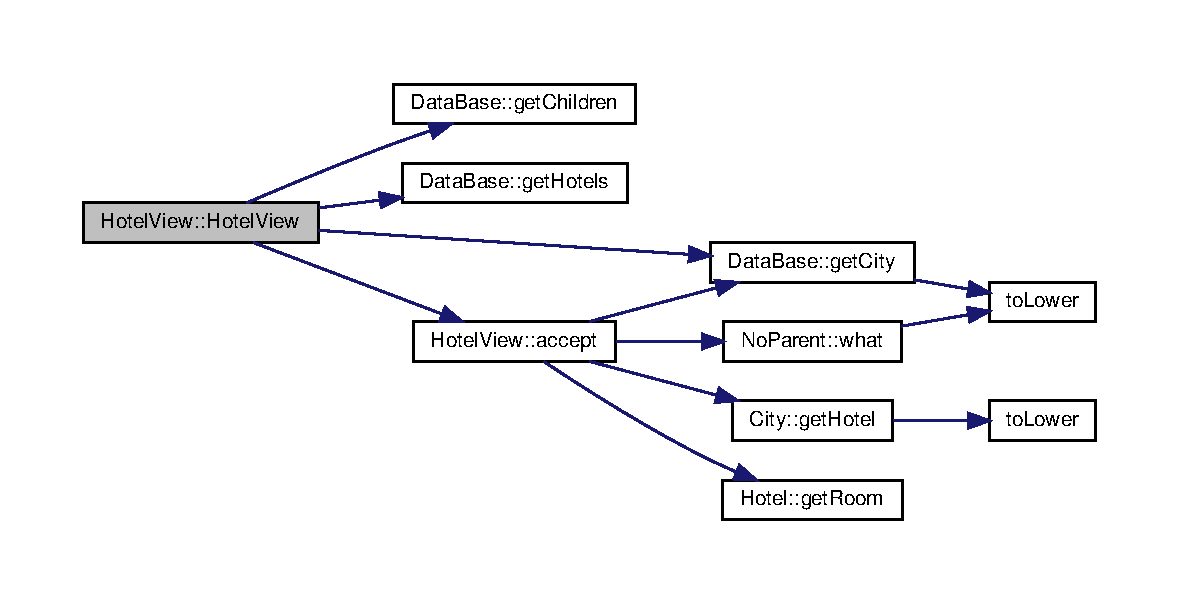
\includegraphics[width=350pt]{class_hotel_view_adba641d84e83365cd5fc499666640dba_cgraph}
\end{center}
\end{figure}


\subsection{Member Function Documentation}
\mbox{\Hypertarget{class_hotel_view_a88805d7379290f2540206d384ef962a1}\label{class_hotel_view_a88805d7379290f2540206d384ef962a1}} 
\index{Hotel\+View@{Hotel\+View}!accept@{accept}}
\index{accept@{accept}!Hotel\+View@{Hotel\+View}}
\subsubsection{\texorpdfstring{accept}{accept}}
{\footnotesize\ttfamily void Hotel\+View\+::accept (\begin{DoxyParamCaption}{ }\end{DoxyParamCaption})\hspace{0.3cm}{\ttfamily [protected]}, {\ttfamily [slot]}}

Here is the call graph for this function\+:\nopagebreak
\begin{figure}[H]
\begin{center}
\leavevmode
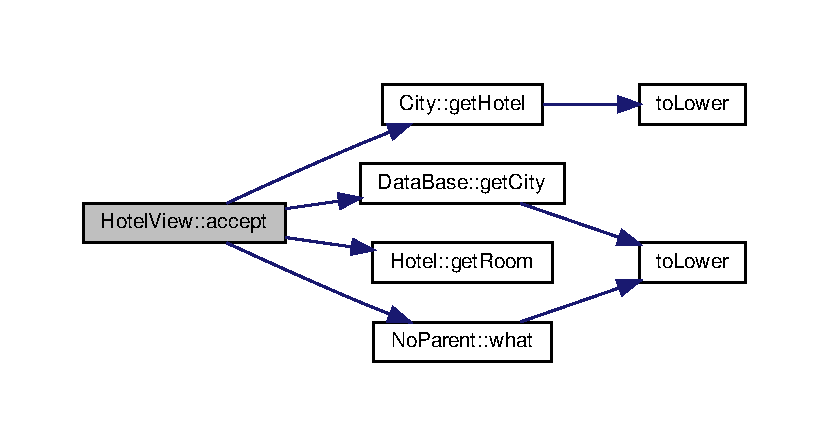
\includegraphics[width=350pt]{class_hotel_view_a88805d7379290f2540206d384ef962a1_cgraph}
\end{center}
\end{figure}
Here is the caller graph for this function\+:\nopagebreak
\begin{figure}[H]
\begin{center}
\leavevmode
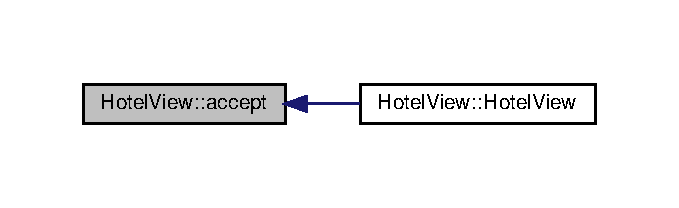
\includegraphics[width=326pt]{class_hotel_view_a88805d7379290f2540206d384ef962a1_icgraph}
\end{center}
\end{figure}


The documentation for this class was generated from the following files\+:\begin{DoxyCompactItemize}
\item 
\hyperlink{hotelview_8h}{hotelview.\+h}\item 
\hyperlink{hotelview_8cpp}{hotelview.\+cpp}\end{DoxyCompactItemize}

\hypertarget{class_no_parent}{}\section{No\+Parent Class Reference}
\label{class_no_parent}\index{No\+Parent@{No\+Parent}}


{\ttfamily \#include $<$hotels.\+h$>$}

\subsection*{Public Member Functions}
\begin{DoxyCompactItemize}
\item 
const char $\ast$ \hyperlink{class_no_parent_aa61c3448b2c6f4e8586590b96bc6ab85}{what} () const
\end{DoxyCompactItemize}


\subsection{Member Function Documentation}
\mbox{\Hypertarget{class_no_parent_aa61c3448b2c6f4e8586590b96bc6ab85}\label{class_no_parent_aa61c3448b2c6f4e8586590b96bc6ab85}} 
\index{No\+Parent@{No\+Parent}!what@{what}}
\index{what@{what}!No\+Parent@{No\+Parent}}
\subsubsection{\texorpdfstring{what()}{what()}}
{\footnotesize\ttfamily const char$\ast$ No\+Parent\+::what (\begin{DoxyParamCaption}{ }\end{DoxyParamCaption}) const\hspace{0.3cm}{\ttfamily [inline]}}

Here is the call graph for this function\+:\nopagebreak
\begin{figure}[H]
\begin{center}
\leavevmode
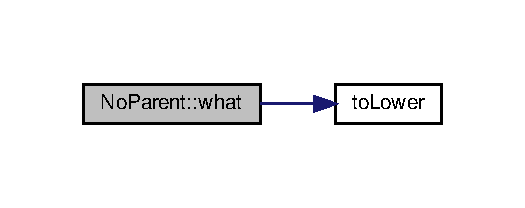
\includegraphics[width=252pt]{class_no_parent_aa61c3448b2c6f4e8586590b96bc6ab85_cgraph}
\end{center}
\end{figure}
Here is the caller graph for this function\+:\nopagebreak
\begin{figure}[H]
\begin{center}
\leavevmode
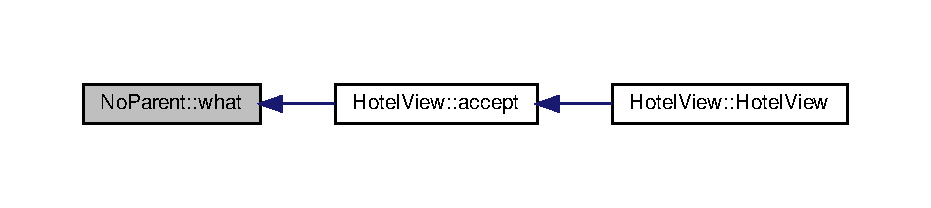
\includegraphics[width=350pt]{class_no_parent_aa61c3448b2c6f4e8586590b96bc6ab85_icgraph}
\end{center}
\end{figure}


The documentation for this class was generated from the following file\+:\begin{DoxyCompactItemize}
\item 
\hyperlink{hotels_8h}{hotels.\+h}\end{DoxyCompactItemize}

\hypertarget{class_no_rooms_available}{}\section{No\+Rooms\+Available Class Reference}
\label{class_no_rooms_available}\index{No\+Rooms\+Available@{No\+Rooms\+Available}}


{\ttfamily \#include $<$hotels.\+h$>$}



Inheritance diagram for No\+Rooms\+Available\+:\nopagebreak
\begin{figure}[H]
\begin{center}
\leavevmode
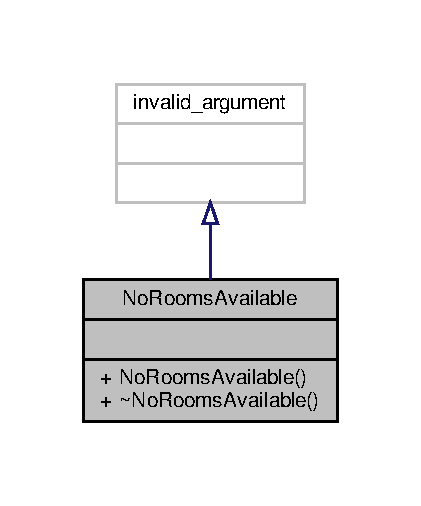
\includegraphics[width=202pt]{class_no_rooms_available__inherit__graph}
\end{center}
\end{figure}
\subsection*{Public Member Functions}
\begin{DoxyCompactItemize}
\item 
\hyperlink{class_no_rooms_available_a16729d574cc4d2c25e5e00b7672a44bd}{No\+Rooms\+Available} ()
\item 
virtual \hyperlink{class_no_rooms_available_af059ca2ab2857824276a1c16426ac13e}{$\sim$\+No\+Rooms\+Available} ()
\end{DoxyCompactItemize}


\subsection{Constructor \& Destructor Documentation}
\mbox{\Hypertarget{class_no_rooms_available_a16729d574cc4d2c25e5e00b7672a44bd}\label{class_no_rooms_available_a16729d574cc4d2c25e5e00b7672a44bd}} 
\index{No\+Rooms\+Available@{No\+Rooms\+Available}!No\+Rooms\+Available@{No\+Rooms\+Available}}
\index{No\+Rooms\+Available@{No\+Rooms\+Available}!No\+Rooms\+Available@{No\+Rooms\+Available}}
\subsubsection{\texorpdfstring{No\+Rooms\+Available()}{NoRoomsAvailable()}}
{\footnotesize\ttfamily No\+Rooms\+Available\+::\+No\+Rooms\+Available (\begin{DoxyParamCaption}{ }\end{DoxyParamCaption})\hspace{0.3cm}{\ttfamily [inline]}}

\mbox{\Hypertarget{class_no_rooms_available_af059ca2ab2857824276a1c16426ac13e}\label{class_no_rooms_available_af059ca2ab2857824276a1c16426ac13e}} 
\index{No\+Rooms\+Available@{No\+Rooms\+Available}!````~No\+Rooms\+Available@{$\sim$\+No\+Rooms\+Available}}
\index{````~No\+Rooms\+Available@{$\sim$\+No\+Rooms\+Available}!No\+Rooms\+Available@{No\+Rooms\+Available}}
\subsubsection{\texorpdfstring{$\sim$\+No\+Rooms\+Available()}{~NoRoomsAvailable()}}
{\footnotesize\ttfamily No\+Rooms\+Available\+::$\sim$\+No\+Rooms\+Available (\begin{DoxyParamCaption}{ }\end{DoxyParamCaption})\hspace{0.3cm}{\ttfamily [virtual]}}



The documentation for this class was generated from the following files\+:\begin{DoxyCompactItemize}
\item 
\hyperlink{hotels_8h}{hotels.\+h}\item 
\hyperlink{hotels_8cpp}{hotels.\+cpp}\end{DoxyCompactItemize}

\hypertarget{structqt__meta__stringdata___hotel_view__t}{}\section{qt\+\_\+meta\+\_\+stringdata\+\_\+\+Hotel\+View\+\_\+t Struct Reference}
\label{structqt__meta__stringdata___hotel_view__t}\index{qt\+\_\+meta\+\_\+stringdata\+\_\+\+Hotel\+View\+\_\+t@{qt\+\_\+meta\+\_\+stringdata\+\_\+\+Hotel\+View\+\_\+t}}
\subsection*{Public Attributes}
\begin{DoxyCompactItemize}
\item 
Q\+Byte\+Array\+Data \hyperlink{structqt__meta__stringdata___hotel_view__t_ad335c1e660c3960878dc3e598403537b}{data} \mbox{[}3\mbox{]}
\item 
char \hyperlink{structqt__meta__stringdata___hotel_view__t_af67aa19cb75af7e8f2eb22ea7b41968c}{stringdata0} \mbox{[}18\mbox{]}
\end{DoxyCompactItemize}


\subsection{Member Data Documentation}
\mbox{\Hypertarget{structqt__meta__stringdata___hotel_view__t_ad335c1e660c3960878dc3e598403537b}\label{structqt__meta__stringdata___hotel_view__t_ad335c1e660c3960878dc3e598403537b}} 
\index{qt\+\_\+meta\+\_\+stringdata\+\_\+\+Hotel\+View\+\_\+t@{qt\+\_\+meta\+\_\+stringdata\+\_\+\+Hotel\+View\+\_\+t}!data@{data}}
\index{data@{data}!qt\+\_\+meta\+\_\+stringdata\+\_\+\+Hotel\+View\+\_\+t@{qt\+\_\+meta\+\_\+stringdata\+\_\+\+Hotel\+View\+\_\+t}}
\subsubsection{\texorpdfstring{data}{data}}
{\footnotesize\ttfamily Q\+Byte\+Array\+Data qt\+\_\+meta\+\_\+stringdata\+\_\+\+Hotel\+View\+\_\+t\+::data}

\mbox{\Hypertarget{structqt__meta__stringdata___hotel_view__t_af67aa19cb75af7e8f2eb22ea7b41968c}\label{structqt__meta__stringdata___hotel_view__t_af67aa19cb75af7e8f2eb22ea7b41968c}} 
\index{qt\+\_\+meta\+\_\+stringdata\+\_\+\+Hotel\+View\+\_\+t@{qt\+\_\+meta\+\_\+stringdata\+\_\+\+Hotel\+View\+\_\+t}!stringdata0@{stringdata0}}
\index{stringdata0@{stringdata0}!qt\+\_\+meta\+\_\+stringdata\+\_\+\+Hotel\+View\+\_\+t@{qt\+\_\+meta\+\_\+stringdata\+\_\+\+Hotel\+View\+\_\+t}}
\subsubsection{\texorpdfstring{stringdata0}{stringdata0}}
{\footnotesize\ttfamily char qt\+\_\+meta\+\_\+stringdata\+\_\+\+Hotel\+View\+\_\+t\+::stringdata0}



The documentation for this struct was generated from the following file\+:\begin{DoxyCompactItemize}
\item 
\hyperlink{moc__hotel_view_8cpp}{moc\+\_\+hotelview.\+cpp}\end{DoxyCompactItemize}

\hypertarget{structqt__meta__stringdata___results_view__t}{}\section{qt\+\_\+meta\+\_\+stringdata\+\_\+\+Results\+View\+\_\+t Struct Reference}
\label{structqt__meta__stringdata___results_view__t}\index{qt\+\_\+meta\+\_\+stringdata\+\_\+\+Results\+View\+\_\+t@{qt\+\_\+meta\+\_\+stringdata\+\_\+\+Results\+View\+\_\+t}}
\subsection*{Public Attributes}
\begin{DoxyCompactItemize}
\item 
Q\+Byte\+Array\+Data \hyperlink{structqt__meta__stringdata___results_view__t_aed28e6e700a8f859c365b6ce6230e12a}{data} \mbox{[}1\mbox{]}
\item 
char \hyperlink{structqt__meta__stringdata___results_view__t_af9d482d0f056d3634500b24b5e33cc34}{stringdata0} \mbox{[}12\mbox{]}
\end{DoxyCompactItemize}


\subsection{Member Data Documentation}
\mbox{\Hypertarget{structqt__meta__stringdata___results_view__t_aed28e6e700a8f859c365b6ce6230e12a}\label{structqt__meta__stringdata___results_view__t_aed28e6e700a8f859c365b6ce6230e12a}} 
\index{qt\+\_\+meta\+\_\+stringdata\+\_\+\+Results\+View\+\_\+t@{qt\+\_\+meta\+\_\+stringdata\+\_\+\+Results\+View\+\_\+t}!data@{data}}
\index{data@{data}!qt\+\_\+meta\+\_\+stringdata\+\_\+\+Results\+View\+\_\+t@{qt\+\_\+meta\+\_\+stringdata\+\_\+\+Results\+View\+\_\+t}}
\subsubsection{\texorpdfstring{data}{data}}
{\footnotesize\ttfamily Q\+Byte\+Array\+Data qt\+\_\+meta\+\_\+stringdata\+\_\+\+Results\+View\+\_\+t\+::data\mbox{[}1\mbox{]}}

\mbox{\Hypertarget{structqt__meta__stringdata___results_view__t_af9d482d0f056d3634500b24b5e33cc34}\label{structqt__meta__stringdata___results_view__t_af9d482d0f056d3634500b24b5e33cc34}} 
\index{qt\+\_\+meta\+\_\+stringdata\+\_\+\+Results\+View\+\_\+t@{qt\+\_\+meta\+\_\+stringdata\+\_\+\+Results\+View\+\_\+t}!stringdata0@{stringdata0}}
\index{stringdata0@{stringdata0}!qt\+\_\+meta\+\_\+stringdata\+\_\+\+Results\+View\+\_\+t@{qt\+\_\+meta\+\_\+stringdata\+\_\+\+Results\+View\+\_\+t}}
\subsubsection{\texorpdfstring{stringdata0}{stringdata0}}
{\footnotesize\ttfamily char qt\+\_\+meta\+\_\+stringdata\+\_\+\+Results\+View\+\_\+t\+::stringdata0\mbox{[}12\mbox{]}}



The documentation for this struct was generated from the following file\+:\begin{DoxyCompactItemize}
\item 
\hyperlink{moc__resultsview_8cpp}{moc\+\_\+resultsview.\+cpp}\end{DoxyCompactItemize}

\hypertarget{class_reservation}{}\section{Reservation Class Reference}
\label{class_reservation}\index{Reservation@{Reservation}}


{\ttfamily \#include $<$hotels.\+h$>$}

\subsection*{Public Member Functions}
\begin{DoxyCompactItemize}
\item 
\hyperlink{class_reservation_ac6d26e98f82dcb33a52b64719160fb82}{Reservation} (Q\+Date m\+\_\+first\+Day, Q\+Date m\+\_\+last\+Day, string m\+\_\+name, string m\+\_\+surname, \hyperlink{class_room}{Room} $\ast$m\+\_\+parent)
\item 
\hyperlink{class_room}{Room} \& \hyperlink{class_reservation_ae2c3cb8475f8649e3d44c076d6340c2c}{get\+Parent} () const
\item 
string \hyperlink{class_reservation_a7187041bfd3814ea69f0c51aabfed8ae}{to\+String} ()
\end{DoxyCompactItemize}
\subsection*{Friends}
\begin{DoxyCompactItemize}
\item 
ostream \& \hyperlink{class_reservation_ac5cc5f8866d66ef4e1c74dbc74380070}{operator$<$$<$} (ostream \&os, const \hyperlink{class_reservation}{Reservation} \&rsv)
\end{DoxyCompactItemize}


\subsection{Constructor \& Destructor Documentation}
\mbox{\Hypertarget{class_reservation_ac6d26e98f82dcb33a52b64719160fb82}\label{class_reservation_ac6d26e98f82dcb33a52b64719160fb82}} 
\index{Reservation@{Reservation}!Reservation@{Reservation}}
\index{Reservation@{Reservation}!Reservation@{Reservation}}
\subsubsection{\texorpdfstring{Reservation()}{Reservation()}}
{\footnotesize\ttfamily Reservation\+::\+Reservation (\begin{DoxyParamCaption}\item[{Q\+Date}]{m\+\_\+first\+Day,  }\item[{Q\+Date}]{m\+\_\+last\+Day,  }\item[{string}]{m\+\_\+name,  }\item[{string}]{m\+\_\+surname,  }\item[{\hyperlink{class_room}{Room} $\ast$}]{m\+\_\+parent }\end{DoxyParamCaption})}

Here is the call graph for this function\+:\nopagebreak
\begin{figure}[H]
\begin{center}
\leavevmode
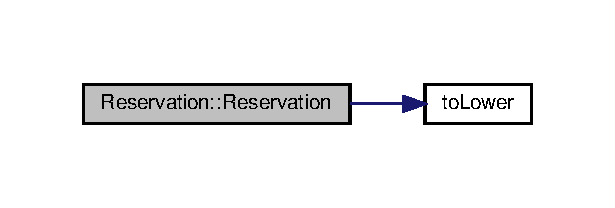
\includegraphics[width=295pt]{class_reservation_ac6d26e98f82dcb33a52b64719160fb82_cgraph}
\end{center}
\end{figure}


\subsection{Member Function Documentation}
\mbox{\Hypertarget{class_reservation_ae2c3cb8475f8649e3d44c076d6340c2c}\label{class_reservation_ae2c3cb8475f8649e3d44c076d6340c2c}} 
\index{Reservation@{Reservation}!get\+Parent@{get\+Parent}}
\index{get\+Parent@{get\+Parent}!Reservation@{Reservation}}
\subsubsection{\texorpdfstring{get\+Parent()}{getParent()}}
{\footnotesize\ttfamily \hyperlink{class_room}{Room}\& Reservation\+::get\+Parent (\begin{DoxyParamCaption}{ }\end{DoxyParamCaption}) const\hspace{0.3cm}{\ttfamily [inline]}}

Here is the call graph for this function\+:\nopagebreak
\begin{figure}[H]
\begin{center}
\leavevmode
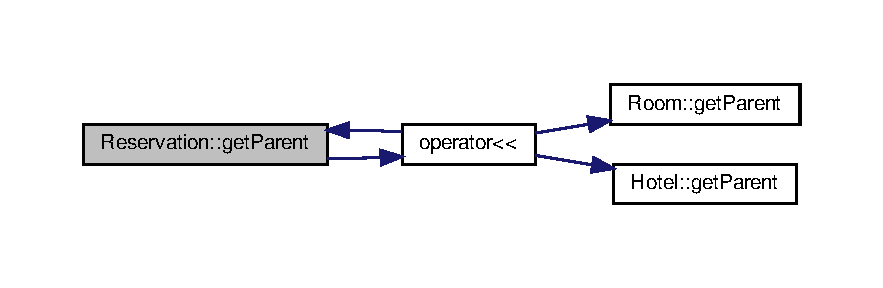
\includegraphics[width=350pt]{class_reservation_ae2c3cb8475f8649e3d44c076d6340c2c_cgraph}
\end{center}
\end{figure}
Here is the caller graph for this function\+:\nopagebreak
\begin{figure}[H]
\begin{center}
\leavevmode
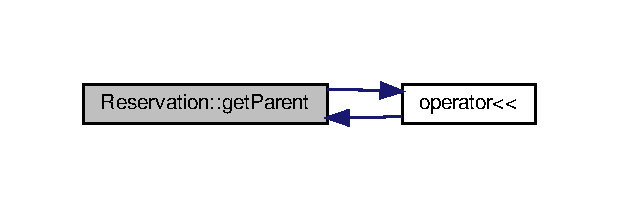
\includegraphics[width=297pt]{class_reservation_ae2c3cb8475f8649e3d44c076d6340c2c_icgraph}
\end{center}
\end{figure}
\mbox{\Hypertarget{class_reservation_a7187041bfd3814ea69f0c51aabfed8ae}\label{class_reservation_a7187041bfd3814ea69f0c51aabfed8ae}} 
\index{Reservation@{Reservation}!to\+String@{to\+String}}
\index{to\+String@{to\+String}!Reservation@{Reservation}}
\subsubsection{\texorpdfstring{to\+String()}{toString()}}
{\footnotesize\ttfamily string Reservation\+::to\+String (\begin{DoxyParamCaption}{ }\end{DoxyParamCaption})}



\subsection{Friends And Related Function Documentation}
\mbox{\Hypertarget{class_reservation_ac5cc5f8866d66ef4e1c74dbc74380070}\label{class_reservation_ac5cc5f8866d66ef4e1c74dbc74380070}} 
\index{Reservation@{Reservation}!operator$<$$<$@{operator$<$$<$}}
\index{operator$<$$<$@{operator$<$$<$}!Reservation@{Reservation}}
\subsubsection{\texorpdfstring{operator$<$$<$}{operator<<}}
{\footnotesize\ttfamily ostream\& operator$<$$<$ (\begin{DoxyParamCaption}\item[{ostream \&}]{os,  }\item[{const \hyperlink{class_reservation}{Reservation} \&}]{rsv }\end{DoxyParamCaption})\hspace{0.3cm}{\ttfamily [friend]}}



The documentation for this class was generated from the following files\+:\begin{DoxyCompactItemize}
\item 
\hyperlink{hotels_8h}{hotels.\+h}\item 
\hyperlink{hotels_8cpp}{hotels.\+cpp}\end{DoxyCompactItemize}

\hypertarget{class_results_view}{}\section{Results\+View Class Reference}
\label{class_results_view}\index{Results\+View@{Results\+View}}


{\ttfamily \#include $<$resultsview.\+h$>$}



Inheritance diagram for Results\+View\+:\nopagebreak
\begin{figure}[H]
\begin{center}
\leavevmode
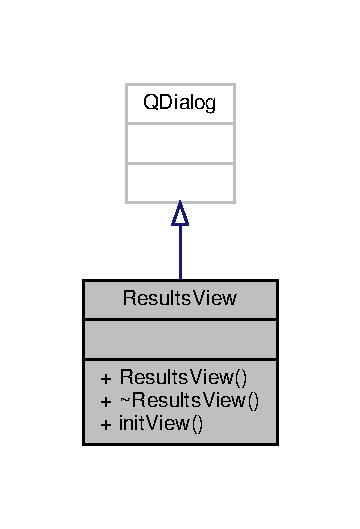
\includegraphics[width=173pt]{class_results_view__inherit__graph}
\end{center}
\end{figure}
\subsection*{Public Member Functions}
\begin{DoxyCompactItemize}
\item 
\hyperlink{class_results_view_a1019cb09ad177a74227ea30e6630e4bf}{Results\+View} (\hyperlink{class_data_base}{Data\+Base} $\ast$m\+\_\+db, std\+::string sur\+Name\+Name, Q\+Widget $\ast$parent=0)
\item 
\hyperlink{class_results_view_af9caa8995848c6e05e8486ad1aac8856}{$\sim$\+Results\+View} ()
\item 
void \hyperlink{class_results_view_ad21cd6811c5b0e4d862563962fbe09d3}{init\+View} ()
\end{DoxyCompactItemize}


\subsection{Constructor \& Destructor Documentation}
\mbox{\Hypertarget{class_results_view_a1019cb09ad177a74227ea30e6630e4bf}\label{class_results_view_a1019cb09ad177a74227ea30e6630e4bf}} 
\index{Results\+View@{Results\+View}!Results\+View@{Results\+View}}
\index{Results\+View@{Results\+View}!Results\+View@{Results\+View}}
\subsubsection{\texorpdfstring{Results\+View()}{ResultsView()}}
{\footnotesize\ttfamily Results\+View\+::\+Results\+View (\begin{DoxyParamCaption}\item[{\hyperlink{class_data_base}{Data\+Base} $\ast$}]{m\+\_\+db,  }\item[{std\+::string}]{sur\+Name\+Name,  }\item[{Q\+Widget $\ast$}]{parent = {\ttfamily 0} }\end{DoxyParamCaption})\hspace{0.3cm}{\ttfamily [explicit]}}

Here is the call graph for this function\+:\nopagebreak
\begin{figure}[H]
\begin{center}
\leavevmode
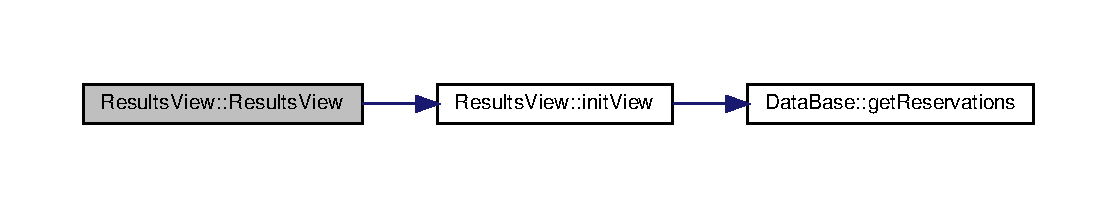
\includegraphics[width=350pt]{class_results_view_a1019cb09ad177a74227ea30e6630e4bf_cgraph}
\end{center}
\end{figure}
\mbox{\Hypertarget{class_results_view_af9caa8995848c6e05e8486ad1aac8856}\label{class_results_view_af9caa8995848c6e05e8486ad1aac8856}} 
\index{Results\+View@{Results\+View}!````~Results\+View@{$\sim$\+Results\+View}}
\index{````~Results\+View@{$\sim$\+Results\+View}!Results\+View@{Results\+View}}
\subsubsection{\texorpdfstring{$\sim$\+Results\+View()}{~ResultsView()}}
{\footnotesize\ttfamily Results\+View\+::$\sim$\+Results\+View (\begin{DoxyParamCaption}{ }\end{DoxyParamCaption})\hspace{0.3cm}{\ttfamily [inline]}}

Here is the call graph for this function\+:\nopagebreak
\begin{figure}[H]
\begin{center}
\leavevmode
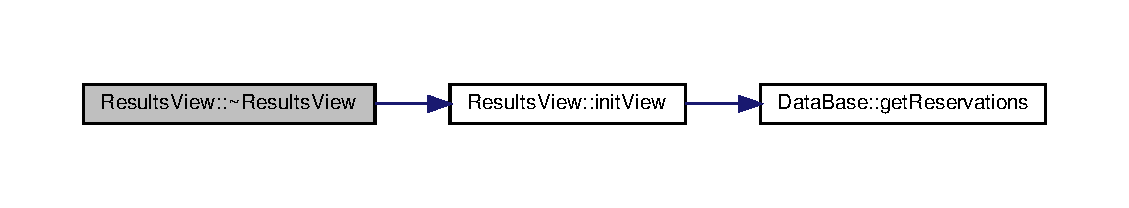
\includegraphics[width=350pt]{class_results_view_af9caa8995848c6e05e8486ad1aac8856_cgraph}
\end{center}
\end{figure}


\subsection{Member Function Documentation}
\mbox{\Hypertarget{class_results_view_ad21cd6811c5b0e4d862563962fbe09d3}\label{class_results_view_ad21cd6811c5b0e4d862563962fbe09d3}} 
\index{Results\+View@{Results\+View}!init\+View@{init\+View}}
\index{init\+View@{init\+View}!Results\+View@{Results\+View}}
\subsubsection{\texorpdfstring{init\+View()}{initView()}}
{\footnotesize\ttfamily void Results\+View\+::init\+View (\begin{DoxyParamCaption}{ }\end{DoxyParamCaption})}

Here is the call graph for this function\+:\nopagebreak
\begin{figure}[H]
\begin{center}
\leavevmode
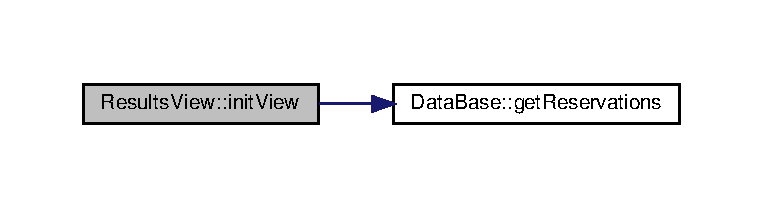
\includegraphics[width=350pt]{class_results_view_ad21cd6811c5b0e4d862563962fbe09d3_cgraph}
\end{center}
\end{figure}
Here is the caller graph for this function\+:\nopagebreak
\begin{figure}[H]
\begin{center}
\leavevmode
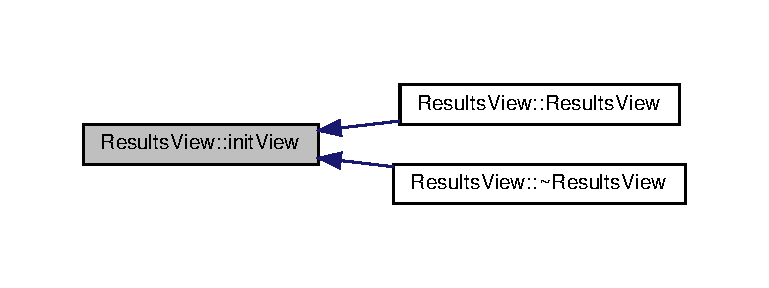
\includegraphics[width=350pt]{class_results_view_ad21cd6811c5b0e4d862563962fbe09d3_icgraph}
\end{center}
\end{figure}


The documentation for this class was generated from the following files\+:\begin{DoxyCompactItemize}
\item 
\hyperlink{resultsview_8h}{resultsview.\+h}\item 
\hyperlink{resultsview_8cpp}{resultsview.\+cpp}\end{DoxyCompactItemize}

\hypertarget{class_room}{}\section{Room Class Reference}
\label{class_room}\index{Room@{Room}}


{\ttfamily \#include $<$hotels.\+h$>$}

\subsection*{Public Member Functions}
\begin{DoxyCompactItemize}
\item 
\hyperlink{class_room_a588e59f9543f9e78cde2b4a812535719}{Room} (int m\+\_\+number, \hyperlink{class_hotel}{Hotel} $\ast$m\+\_\+parent)
\item 
\hyperlink{class_room_a67d5da09983cc53097807fd43ba5481a}{$\sim$\+Room} ()
\item 
\hyperlink{class_hotel}{Hotel} \& \hyperlink{class_room_aa1b182693c0bae407f74fcb2815d1605}{get\+Parent} ()
\item 
vector$<$ Q\+Date $>$ \& \hyperlink{class_room_a92a34c55f5109a669b164653d391a5eb}{get\+Free\+Dates} ()
\item 
\hyperlink{class_room_a41563a17c78b8dcebaaae4d07dd3537c}{operator int} ()
\item 
bool \hyperlink{class_room_a72182e2599a2aac3312ef8aa040803af}{is\+Free} (Q\+Date first\+Day, Q\+Date last\+Day)
\item 
void \hyperlink{class_room_a01b6361bb54fe5f61cf7c768e60bf6fc}{book} (Q\+Date m\+\_\+first\+Day, Q\+Date m\+\_\+last\+Day, string m\+\_\+name, string m\+\_\+surname)
\item 
void \hyperlink{class_room_aa606091a9d9aad6801675384c77d6634}{add\+Reservation} (string sur\+Name\+Name, \hyperlink{class_reservation}{Reservation} $\ast$rsv)
\item 
bool \hyperlink{class_room_ad05581dd91f323159ee69d52197ed595}{has\+Reservations} () const
\item 
void \hyperlink{class_room_af606f87948de7df87296b3c720500cb7}{show\+Reservations} (ostream \&os) const
\item 
vector$<$ string $>$ \hyperlink{class_room_a10d6dafe0c9e42cfaa19c049e0263d99}{get\+Reservations} (string sur\+Name\+Name)
\end{DoxyCompactItemize}


\subsection{Constructor \& Destructor Documentation}
\mbox{\Hypertarget{class_room_a588e59f9543f9e78cde2b4a812535719}\label{class_room_a588e59f9543f9e78cde2b4a812535719}} 
\index{Room@{Room}!Room@{Room}}
\index{Room@{Room}!Room@{Room}}
\subsubsection{\texorpdfstring{Room()}{Room()}}
{\footnotesize\ttfamily Room\+::\+Room (\begin{DoxyParamCaption}\item[{int}]{m\+\_\+number,  }\item[{\hyperlink{class_hotel}{Hotel} $\ast$}]{m\+\_\+parent }\end{DoxyParamCaption})}

Here is the call graph for this function\+:\nopagebreak
\begin{figure}[H]
\begin{center}
\leavevmode
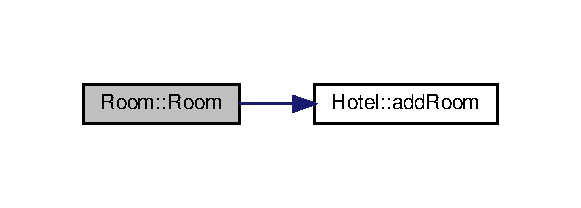
\includegraphics[width=279pt]{class_room_a588e59f9543f9e78cde2b4a812535719_cgraph}
\end{center}
\end{figure}
\mbox{\Hypertarget{class_room_a67d5da09983cc53097807fd43ba5481a}\label{class_room_a67d5da09983cc53097807fd43ba5481a}} 
\index{Room@{Room}!````~Room@{$\sim$\+Room}}
\index{````~Room@{$\sim$\+Room}!Room@{Room}}
\subsubsection{\texorpdfstring{$\sim$\+Room()}{~Room()}}
{\footnotesize\ttfamily Room\+::$\sim$\+Room (\begin{DoxyParamCaption}{ }\end{DoxyParamCaption})\hspace{0.3cm}{\ttfamily [inline]}}



\subsection{Member Function Documentation}
\mbox{\Hypertarget{class_room_aa606091a9d9aad6801675384c77d6634}\label{class_room_aa606091a9d9aad6801675384c77d6634}} 
\index{Room@{Room}!add\+Reservation@{add\+Reservation}}
\index{add\+Reservation@{add\+Reservation}!Room@{Room}}
\subsubsection{\texorpdfstring{add\+Reservation()}{addReservation()}}
{\footnotesize\ttfamily void Room\+::add\+Reservation (\begin{DoxyParamCaption}\item[{string}]{sur\+Name\+Name,  }\item[{\hyperlink{class_reservation}{Reservation} $\ast$}]{rsv }\end{DoxyParamCaption})\hspace{0.3cm}{\ttfamily [inline]}}

\mbox{\Hypertarget{class_room_a01b6361bb54fe5f61cf7c768e60bf6fc}\label{class_room_a01b6361bb54fe5f61cf7c768e60bf6fc}} 
\index{Room@{Room}!book@{book}}
\index{book@{book}!Room@{Room}}
\subsubsection{\texorpdfstring{book()}{book()}}
{\footnotesize\ttfamily void Room\+::book (\begin{DoxyParamCaption}\item[{Q\+Date}]{m\+\_\+first\+Day,  }\item[{Q\+Date}]{m\+\_\+last\+Day,  }\item[{string}]{m\+\_\+name,  }\item[{string}]{m\+\_\+surname }\end{DoxyParamCaption})}

\mbox{\Hypertarget{class_room_a92a34c55f5109a669b164653d391a5eb}\label{class_room_a92a34c55f5109a669b164653d391a5eb}} 
\index{Room@{Room}!get\+Free\+Dates@{get\+Free\+Dates}}
\index{get\+Free\+Dates@{get\+Free\+Dates}!Room@{Room}}
\subsubsection{\texorpdfstring{get\+Free\+Dates()}{getFreeDates()}}
{\footnotesize\ttfamily vector$<$Q\+Date$>$\& Room\+::get\+Free\+Dates (\begin{DoxyParamCaption}{ }\end{DoxyParamCaption})\hspace{0.3cm}{\ttfamily [inline]}}

\mbox{\Hypertarget{class_room_aa1b182693c0bae407f74fcb2815d1605}\label{class_room_aa1b182693c0bae407f74fcb2815d1605}} 
\index{Room@{Room}!get\+Parent@{get\+Parent}}
\index{get\+Parent@{get\+Parent}!Room@{Room}}
\subsubsection{\texorpdfstring{get\+Parent()}{getParent()}}
{\footnotesize\ttfamily \hyperlink{class_hotel}{Hotel}\& Room\+::get\+Parent (\begin{DoxyParamCaption}{ }\end{DoxyParamCaption})\hspace{0.3cm}{\ttfamily [inline]}}

Here is the caller graph for this function\+:\nopagebreak
\begin{figure}[H]
\begin{center}
\leavevmode
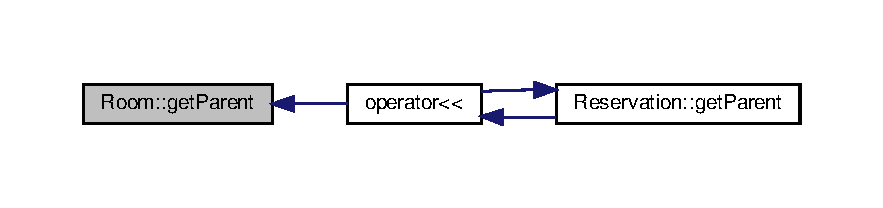
\includegraphics[width=350pt]{class_room_aa1b182693c0bae407f74fcb2815d1605_icgraph}
\end{center}
\end{figure}
\mbox{\Hypertarget{class_room_a10d6dafe0c9e42cfaa19c049e0263d99}\label{class_room_a10d6dafe0c9e42cfaa19c049e0263d99}} 
\index{Room@{Room}!get\+Reservations@{get\+Reservations}}
\index{get\+Reservations@{get\+Reservations}!Room@{Room}}
\subsubsection{\texorpdfstring{get\+Reservations()}{getReservations()}}
{\footnotesize\ttfamily vector$<$string$>$ Room\+::get\+Reservations (\begin{DoxyParamCaption}\item[{string}]{sur\+Name\+Name }\end{DoxyParamCaption})\hspace{0.3cm}{\ttfamily [inline]}}

Here is the call graph for this function\+:\nopagebreak
\begin{figure}[H]
\begin{center}
\leavevmode
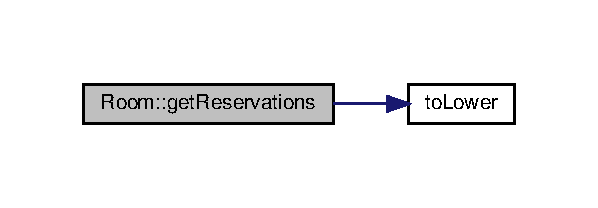
\includegraphics[width=287pt]{class_room_a10d6dafe0c9e42cfaa19c049e0263d99_cgraph}
\end{center}
\end{figure}
\mbox{\Hypertarget{class_room_ad05581dd91f323159ee69d52197ed595}\label{class_room_ad05581dd91f323159ee69d52197ed595}} 
\index{Room@{Room}!has\+Reservations@{has\+Reservations}}
\index{has\+Reservations@{has\+Reservations}!Room@{Room}}
\subsubsection{\texorpdfstring{has\+Reservations()}{hasReservations()}}
{\footnotesize\ttfamily bool Room\+::has\+Reservations (\begin{DoxyParamCaption}{ }\end{DoxyParamCaption}) const\hspace{0.3cm}{\ttfamily [inline]}}

\mbox{\Hypertarget{class_room_a72182e2599a2aac3312ef8aa040803af}\label{class_room_a72182e2599a2aac3312ef8aa040803af}} 
\index{Room@{Room}!is\+Free@{is\+Free}}
\index{is\+Free@{is\+Free}!Room@{Room}}
\subsubsection{\texorpdfstring{is\+Free()}{isFree()}}
{\footnotesize\ttfamily bool Room\+::is\+Free (\begin{DoxyParamCaption}\item[{Q\+Date}]{first\+Day,  }\item[{Q\+Date}]{last\+Day }\end{DoxyParamCaption})}

\mbox{\Hypertarget{class_room_a41563a17c78b8dcebaaae4d07dd3537c}\label{class_room_a41563a17c78b8dcebaaae4d07dd3537c}} 
\index{Room@{Room}!operator int@{operator int}}
\index{operator int@{operator int}!Room@{Room}}
\subsubsection{\texorpdfstring{operator int()}{operator int()}}
{\footnotesize\ttfamily Room\+::operator int (\begin{DoxyParamCaption}{ }\end{DoxyParamCaption})\hspace{0.3cm}{\ttfamily [inline]}, {\ttfamily [explicit]}}

\mbox{\Hypertarget{class_room_af606f87948de7df87296b3c720500cb7}\label{class_room_af606f87948de7df87296b3c720500cb7}} 
\index{Room@{Room}!show\+Reservations@{show\+Reservations}}
\index{show\+Reservations@{show\+Reservations}!Room@{Room}}
\subsubsection{\texorpdfstring{show\+Reservations()}{showReservations()}}
{\footnotesize\ttfamily void Room\+::show\+Reservations (\begin{DoxyParamCaption}\item[{ostream \&}]{os }\end{DoxyParamCaption}) const\hspace{0.3cm}{\ttfamily [inline]}}



The documentation for this class was generated from the following files\+:\begin{DoxyCompactItemize}
\item 
\hyperlink{hotels_8h}{hotels.\+h}\item 
\hyperlink{hotels_8cpp}{hotels.\+cpp}\end{DoxyCompactItemize}

\chapter{File Documentation}
\hypertarget{hotels_8cpp}{}\section{hotels.\+cpp File Reference}
\label{hotels_8cpp}\index{hotels.\+cpp@{hotels.\+cpp}}
{\ttfamily \#include \char`\"{}hotels.\+h\char`\"{}}\newline
{\ttfamily \#include $<$iostream$>$}\newline
{\ttfamily \#include $<$fstream$>$}\newline
{\ttfamily \#include $<$sstream$>$}\newline
{\ttfamily \#include $<$iomanip$>$}\newline
{\ttfamily \#include $<$exception$>$}\newline
Include dependency graph for hotels.\+cpp\+:\nopagebreak
\begin{figure}[H]
\begin{center}
\leavevmode
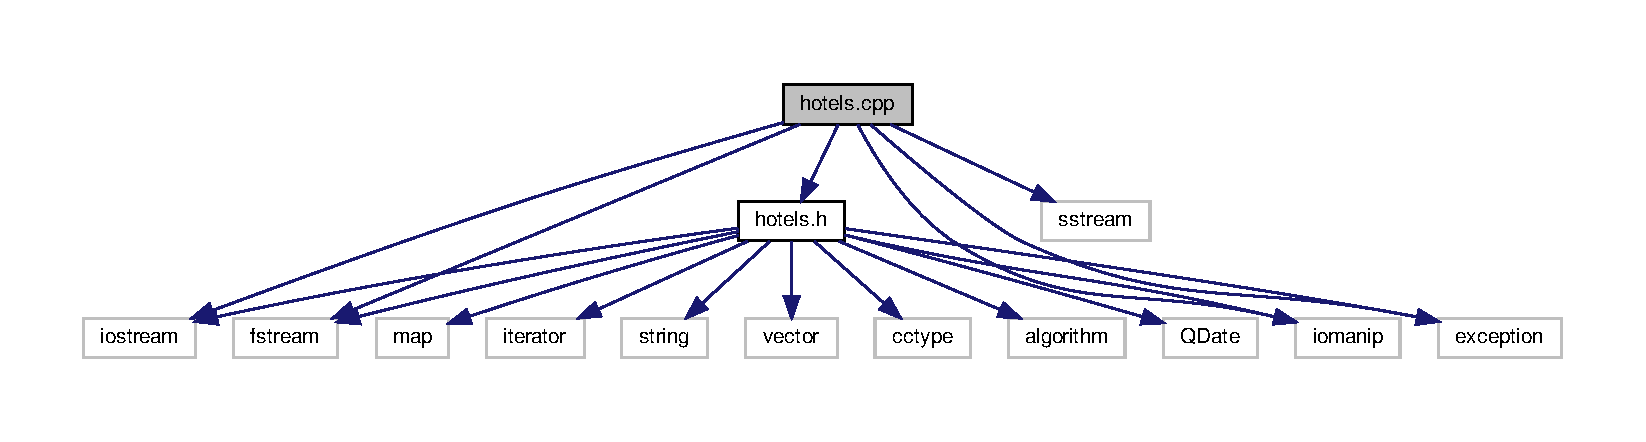
\includegraphics[width=350pt]{hotels_8cpp__incl}
\end{center}
\end{figure}
\subsection*{Functions}
\begin{DoxyCompactItemize}
\item 
string \hyperlink{hotels_8cpp_a637fd73afd1fadd689749ce8ec66e33a}{to\+Lower} (string str)
\item 
ostream \& \hyperlink{hotels_8cpp_ac5cc5f8866d66ef4e1c74dbc74380070}{operator$<$$<$} (ostream \&os, const \hyperlink{class_reservation}{Reservation} \&rsv)
\end{DoxyCompactItemize}


\subsection{Function Documentation}
\mbox{\Hypertarget{hotels_8cpp_ac5cc5f8866d66ef4e1c74dbc74380070}\label{hotels_8cpp_ac5cc5f8866d66ef4e1c74dbc74380070}} 
\index{hotels.\+cpp@{hotels.\+cpp}!operator$<$$<$@{operator$<$$<$}}
\index{operator$<$$<$@{operator$<$$<$}!hotels.\+cpp@{hotels.\+cpp}}
\subsubsection{\texorpdfstring{operator$<$$<$()}{operator<<()}}
{\footnotesize\ttfamily ostream\& operator$<$$<$ (\begin{DoxyParamCaption}\item[{ostream \&}]{os,  }\item[{const \hyperlink{class_reservation}{Reservation} \&}]{rsv }\end{DoxyParamCaption})}

Here is the call graph for this function\+:\nopagebreak
\begin{figure}[H]
\begin{center}
\leavevmode
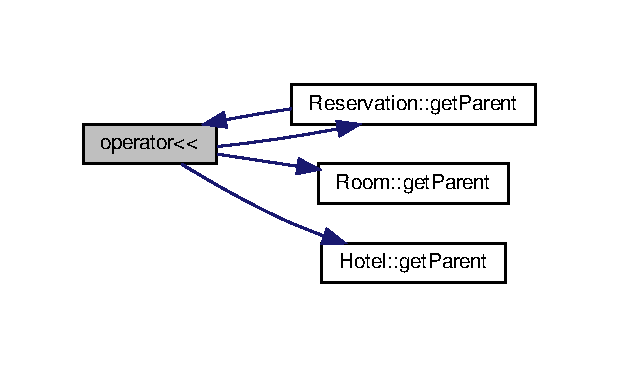
\includegraphics[width=297pt]{hotels_8cpp_ac5cc5f8866d66ef4e1c74dbc74380070_cgraph}
\end{center}
\end{figure}
Here is the caller graph for this function\+:\nopagebreak
\begin{figure}[H]
\begin{center}
\leavevmode
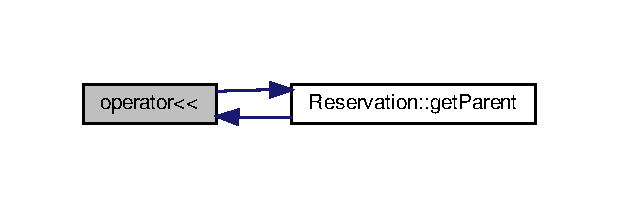
\includegraphics[width=297pt]{hotels_8cpp_ac5cc5f8866d66ef4e1c74dbc74380070_icgraph}
\end{center}
\end{figure}
\mbox{\Hypertarget{hotels_8cpp_a637fd73afd1fadd689749ce8ec66e33a}\label{hotels_8cpp_a637fd73afd1fadd689749ce8ec66e33a}} 
\index{hotels.\+cpp@{hotels.\+cpp}!to\+Lower@{to\+Lower}}
\index{to\+Lower@{to\+Lower}!hotels.\+cpp@{hotels.\+cpp}}
\subsubsection{\texorpdfstring{to\+Lower()}{toLower()}}
{\footnotesize\ttfamily string to\+Lower (\begin{DoxyParamCaption}\item[{string}]{str }\end{DoxyParamCaption})}

Here is the caller graph for this function\+:\nopagebreak
\begin{figure}[H]
\begin{center}
\leavevmode
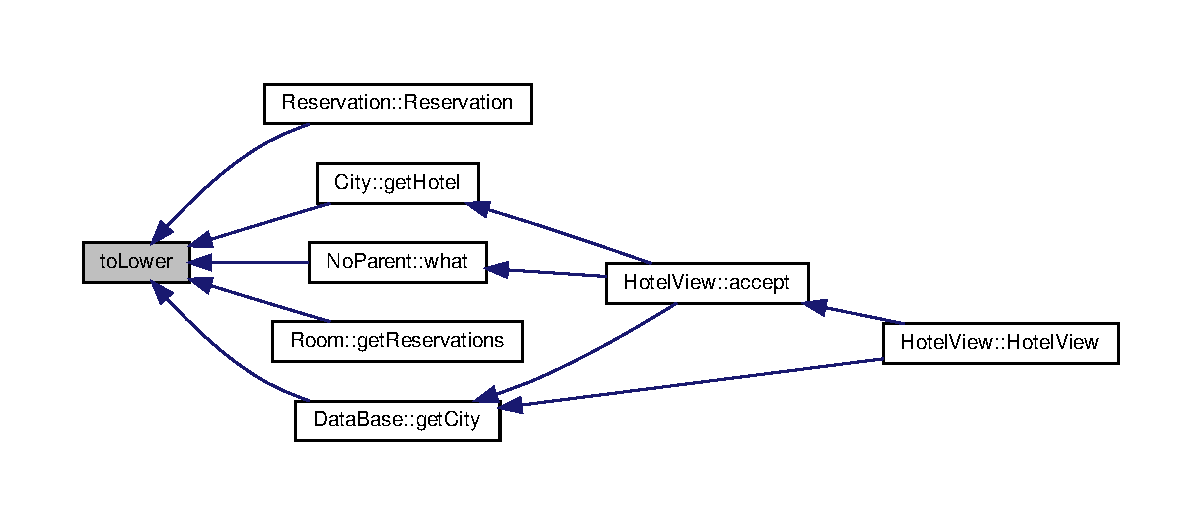
\includegraphics[width=350pt]{hotels_8cpp_a637fd73afd1fadd689749ce8ec66e33a_icgraph}
\end{center}
\end{figure}

\hypertarget{hotels_8h}{}\section{hotels.\+h File Reference}
\label{hotels_8h}\index{hotels.\+h@{hotels.\+h}}
{\ttfamily \#include $<$string$>$}\newline
{\ttfamily \#include $<$vector$>$}\newline
{\ttfamily \#include $<$iostream$>$}\newline
{\ttfamily \#include $<$fstream$>$}\newline
{\ttfamily \#include $<$cctype$>$}\newline
{\ttfamily \#include $<$algorithm$>$}\newline
{\ttfamily \#include $<$iomanip$>$}\newline
{\ttfamily \#include $<$exception$>$}\newline
{\ttfamily \#include $<$Q\+Date$>$}\newline
{\ttfamily \#include $<$map$>$}\newline
{\ttfamily \#include $<$iterator$>$}\newline
Include dependency graph for hotels.\+h\+:\nopagebreak
\begin{figure}[H]
\begin{center}
\leavevmode
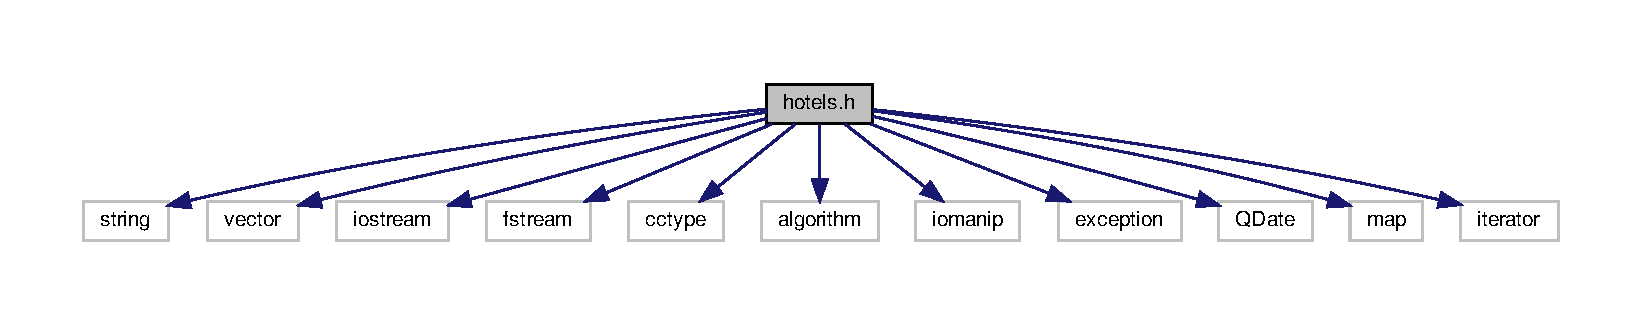
\includegraphics[width=350pt]{hotels_8h__incl}
\end{center}
\end{figure}
This graph shows which files directly or indirectly include this file\+:\nopagebreak
\begin{figure}[H]
\begin{center}
\leavevmode
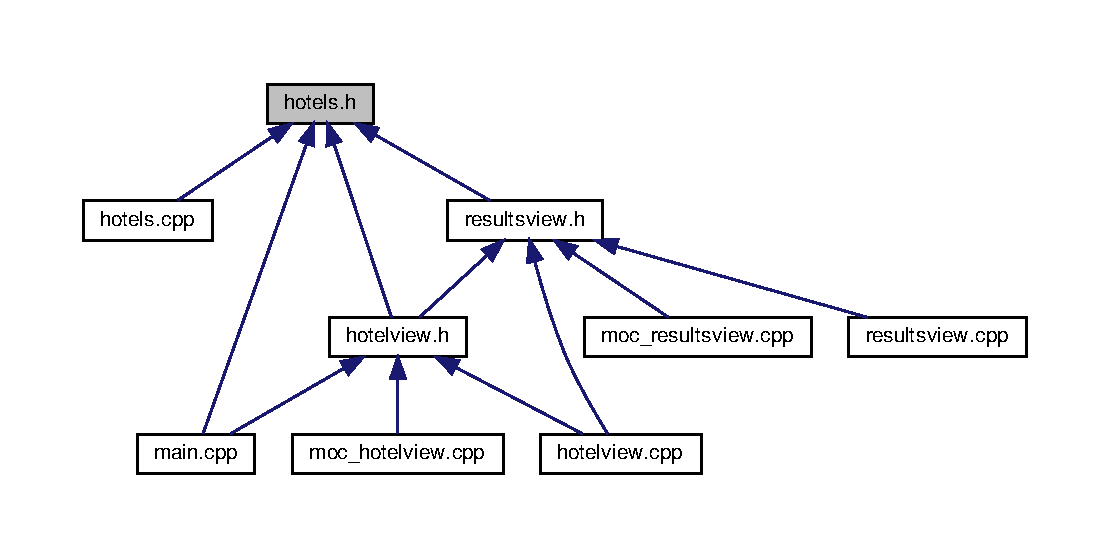
\includegraphics[width=350pt]{hotels_8h__dep__incl}
\end{center}
\end{figure}
\subsection*{Classes}
\begin{DoxyCompactItemize}
\item 
class \hyperlink{class_bad_file_name}{Bad\+File\+Name}
\item 
class \hyperlink{class_bad_city_name}{Bad\+City\+Name}
\item 
class \hyperlink{class_bad_hotel_name}{Bad\+Hotel\+Name}
\item 
class \hyperlink{class_bad_room_number}{Bad\+Room\+Number}
\item 
class \hyperlink{class_no_rooms_available}{No\+Rooms\+Available}
\item 
class \hyperlink{class_no_parent}{No\+Parent}
\item 
class \hyperlink{class_reservation}{Reservation}
\item 
class \hyperlink{class_room}{Room}
\item 
class \hyperlink{class_hotel}{Hotel}
\item 
class \hyperlink{class_city}{City}
\item 
class \hyperlink{class_data_base}{Data\+Base}
\end{DoxyCompactItemize}
\subsection*{Functions}
\begin{DoxyCompactItemize}
\item 
string \hyperlink{hotels_8h_a637fd73afd1fadd689749ce8ec66e33a}{to\+Lower} (string str)
\end{DoxyCompactItemize}


\subsection{Function Documentation}
\mbox{\Hypertarget{hotels_8h_a637fd73afd1fadd689749ce8ec66e33a}\label{hotels_8h_a637fd73afd1fadd689749ce8ec66e33a}} 
\index{hotels.\+h@{hotels.\+h}!to\+Lower@{to\+Lower}}
\index{to\+Lower@{to\+Lower}!hotels.\+h@{hotels.\+h}}
\subsubsection{\texorpdfstring{to\+Lower()}{toLower()}}
{\footnotesize\ttfamily string to\+Lower (\begin{DoxyParamCaption}\item[{string}]{str }\end{DoxyParamCaption})}

Here is the caller graph for this function\+:\nopagebreak
\begin{figure}[H]
\begin{center}
\leavevmode
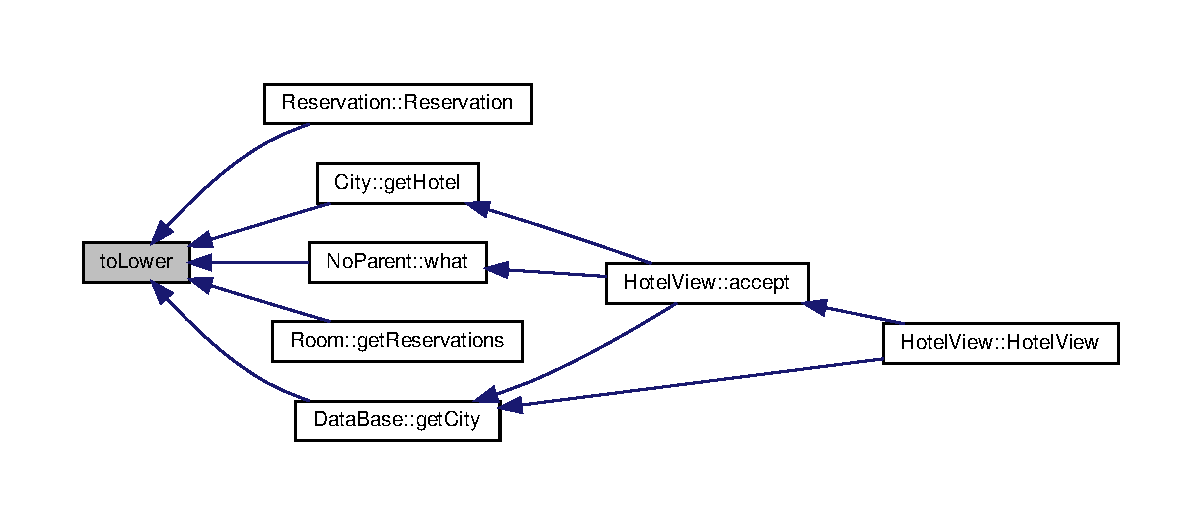
\includegraphics[width=350pt]{hotels_8h_a637fd73afd1fadd689749ce8ec66e33a_icgraph}
\end{center}
\end{figure}

\hypertarget{hotelview_8cpp}{}\section{hotelview.\+cpp File Reference}
\label{hotelview_8cpp}\index{hotelview.\+cpp@{hotelview.\+cpp}}
{\ttfamily \#include \char`\"{}hotelview.\+h\char`\"{}}\newline
{\ttfamily \#include \char`\"{}resultsview.\+h\char`\"{}}\newline
{\ttfamily \#include $<$Q\+Form\+Layout$>$}\newline
{\ttfamily \#include $<$Q\+Date\+Edit$>$}\newline
{\ttfamily \#include $<$Q\+Line\+Edit$>$}\newline
{\ttfamily \#include $<$Q\+Dialog\+Button\+Box$>$}\newline
{\ttfamily \#include $<$Q\+Message\+Box$>$}\newline
{\ttfamily \#include $<$iostream$>$}\newline
{\ttfamily \#include $<$Q\+Combo\+Box$>$}\newline
{\ttfamily \#include $<$Q\+Image$>$}\newline
{\ttfamily \#include $<$Q\+Label$>$}\newline
{\ttfamily \#include $<$Q\+Pixmap$>$}\newline
Include dependency graph for hotelview.\+cpp\+:\nopagebreak
\begin{figure}[H]
\begin{center}
\leavevmode
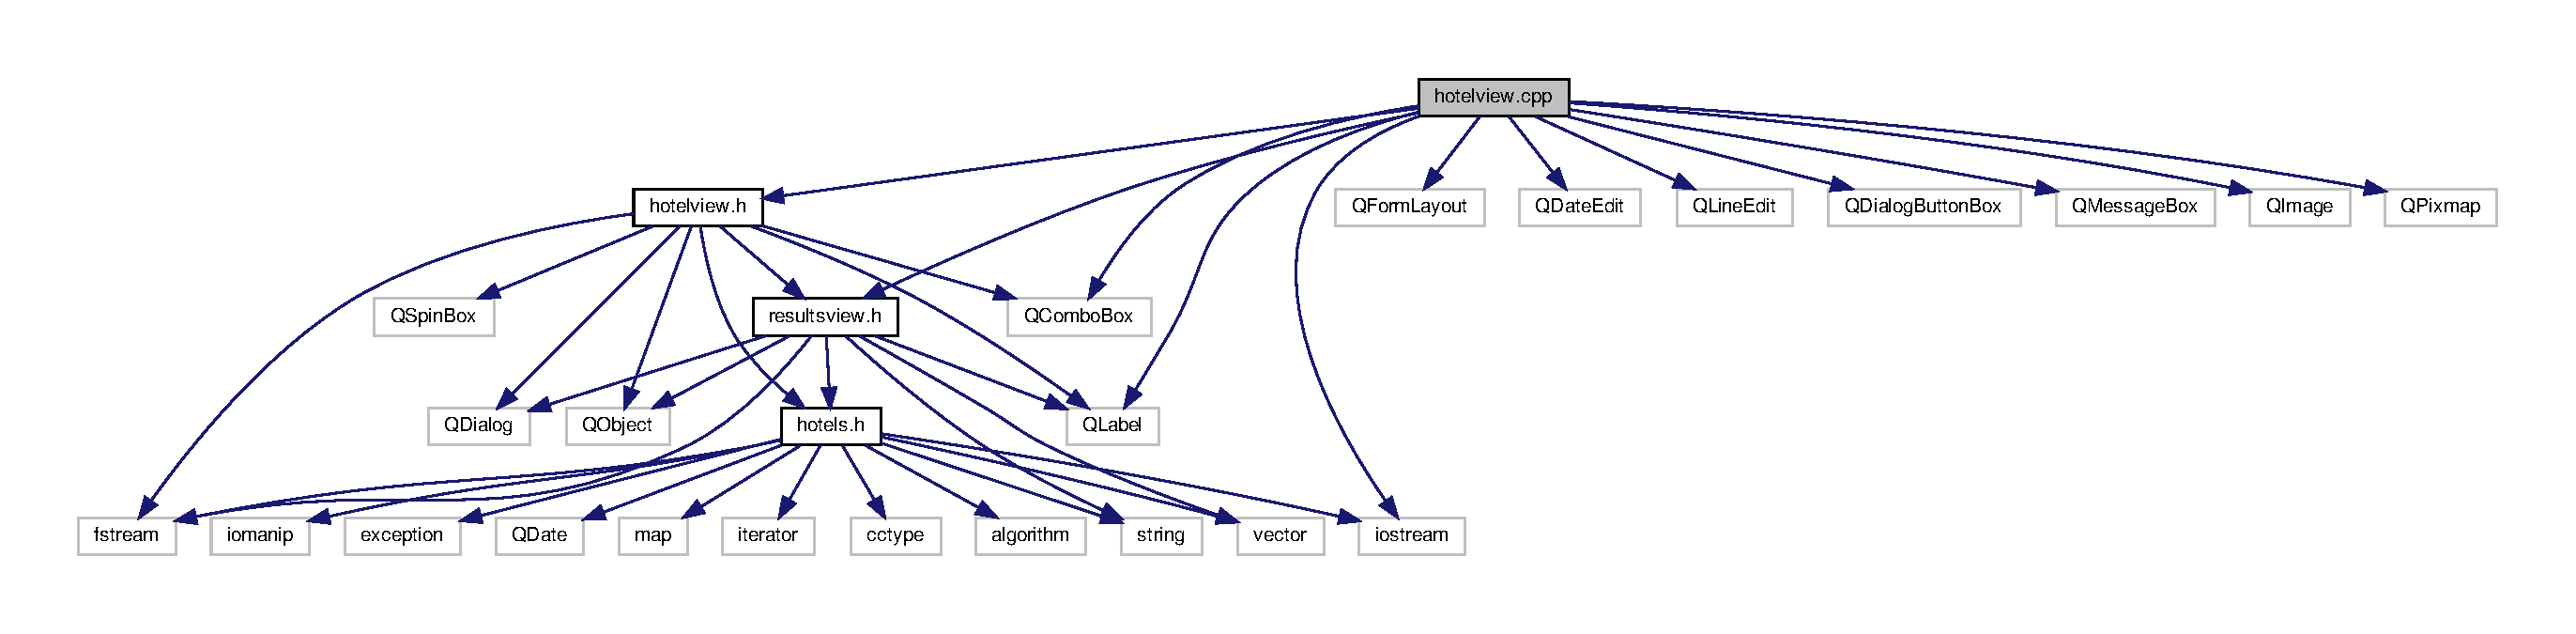
\includegraphics[width=350pt]{hotelview_8cpp__incl}
\end{center}
\end{figure}

\hypertarget{hotelview_8h}{}\section{hotelview.\+h File Reference}
\label{hotelview_8h}\index{hotelview.\+h@{hotelview.\+h}}
{\ttfamily \#include \char`\"{}hotels.\+h\char`\"{}}\newline
{\ttfamily \#include \char`\"{}resultsview.\+h\char`\"{}}\newline
{\ttfamily \#include $<$Q\+Dialog$>$}\newline
{\ttfamily \#include $<$Q\+Spin\+Box$>$}\newline
{\ttfamily \#include $<$Q\+Combo\+Box$>$}\newline
{\ttfamily \#include $<$Q\+Object$>$}\newline
{\ttfamily \#include $<$Q\+Label$>$}\newline
{\ttfamily \#include $<$fstream$>$}\newline
Include dependency graph for hotelview.\+h\+:\nopagebreak
\begin{figure}[H]
\begin{center}
\leavevmode
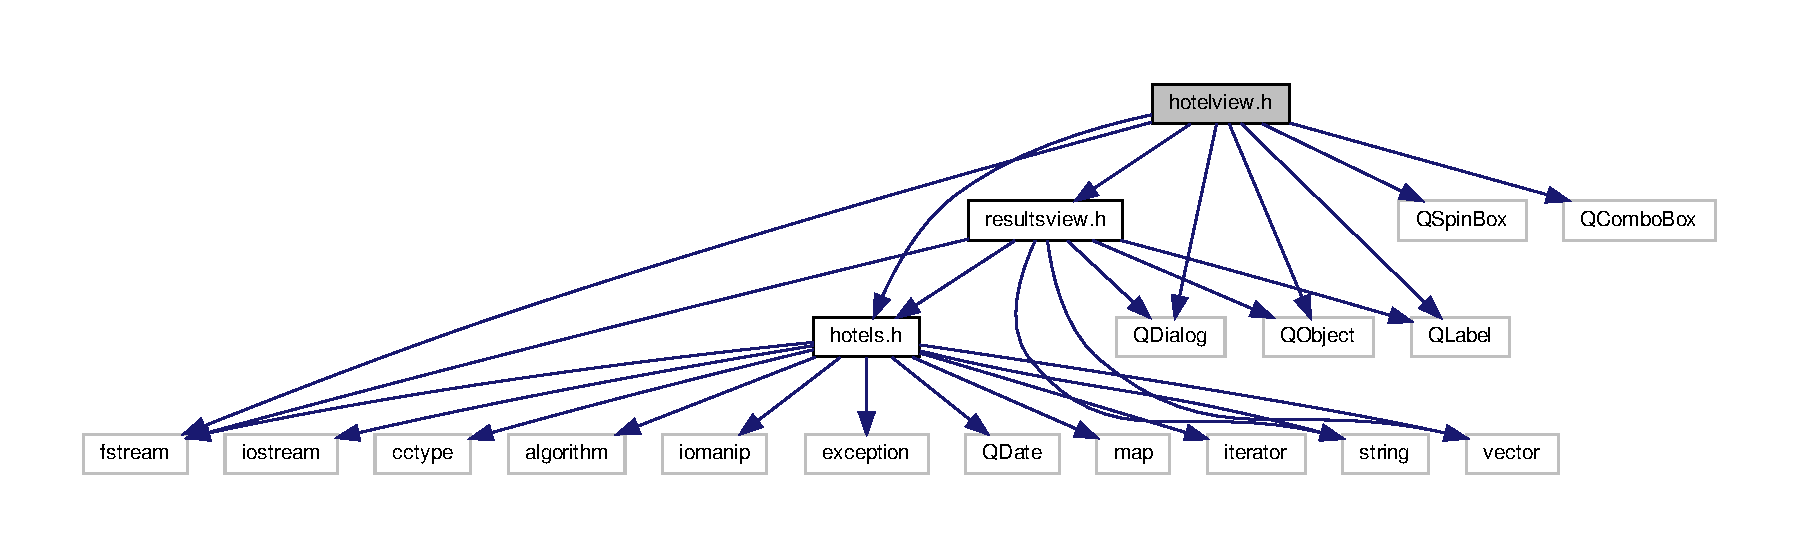
\includegraphics[width=350pt]{hotelview_8h__incl}
\end{center}
\end{figure}
This graph shows which files directly or indirectly include this file\+:\nopagebreak
\begin{figure}[H]
\begin{center}
\leavevmode
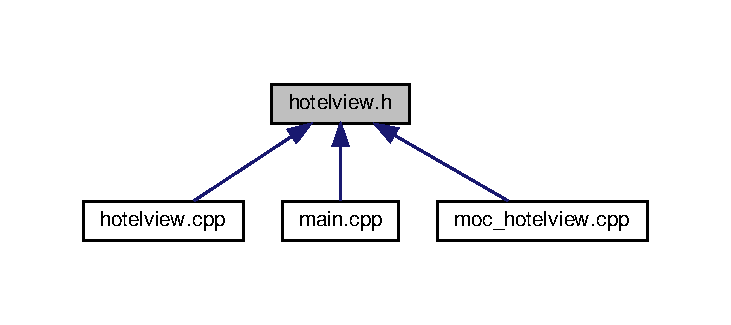
\includegraphics[width=350pt]{hotelview_8h__dep__incl}
\end{center}
\end{figure}
\subsection*{Classes}
\begin{DoxyCompactItemize}
\item 
class \hyperlink{class_hotel_view}{Hotel\+View}
\end{DoxyCompactItemize}
\subsection*{Macros}
\begin{DoxyCompactItemize}
\item 
\#define \hyperlink{hotelview_8h_a1d6183f074b1d214af1b6c563303cdd6}{H\+O\+T\+E\+L\+S\+R\+E\+S\+E\+R\+V\+A\+T\+I\+O\+N\+\_\+\+H\+O\+T\+E\+L\+V\+I\+E\+V\+\_\+}
\end{DoxyCompactItemize}


\subsection{Macro Definition Documentation}
\mbox{\Hypertarget{hotelview_8h_a1d6183f074b1d214af1b6c563303cdd6}\label{hotelview_8h_a1d6183f074b1d214af1b6c563303cdd6}} 
\index{hotelview.\+h@{hotelview.\+h}!H\+O\+T\+E\+L\+S\+R\+E\+S\+E\+R\+V\+A\+T\+I\+O\+N\+\_\+\+H\+O\+T\+E\+L\+V\+I\+E\+V\+\_\+@{H\+O\+T\+E\+L\+S\+R\+E\+S\+E\+R\+V\+A\+T\+I\+O\+N\+\_\+\+H\+O\+T\+E\+L\+V\+I\+E\+V\+\_\+}}
\index{H\+O\+T\+E\+L\+S\+R\+E\+S\+E\+R\+V\+A\+T\+I\+O\+N\+\_\+\+H\+O\+T\+E\+L\+V\+I\+E\+V\+\_\+@{H\+O\+T\+E\+L\+S\+R\+E\+S\+E\+R\+V\+A\+T\+I\+O\+N\+\_\+\+H\+O\+T\+E\+L\+V\+I\+E\+V\+\_\+}!hotelview.\+h@{hotelview.\+h}}
\subsubsection{\texorpdfstring{H\+O\+T\+E\+L\+S\+R\+E\+S\+E\+R\+V\+A\+T\+I\+O\+N\+\_\+\+H\+O\+T\+E\+L\+V\+I\+E\+V\+\_\+}{HOTELSRESERVATION\_HOTELVIEV\_}}
{\footnotesize\ttfamily \#define H\+O\+T\+E\+L\+S\+R\+E\+S\+E\+R\+V\+A\+T\+I\+O\+N\+\_\+\+H\+O\+T\+E\+L\+V\+I\+E\+V\+\_\+}


\hypertarget{main_8cpp}{}\section{main.\+cpp File Reference}
\label{main_8cpp}\index{main.\+cpp@{main.\+cpp}}
{\ttfamily \#include \char`\"{}hotelview.\+h\char`\"{}}\newline
{\ttfamily \#include \char`\"{}hotels.\+h\char`\"{}}\newline
{\ttfamily \#include $<$iostream$>$}\newline
{\ttfamily \#include $<$fstream$>$}\newline
{\ttfamily \#include $<$cctype$>$}\newline
{\ttfamily \#include $<$exception$>$}\newline
{\ttfamily \#include $<$Q\+Debug$>$}\newline
{\ttfamily \#include $<$Qt\+Widgets$>$}\newline
Include dependency graph for main.\+cpp\+:\nopagebreak
\begin{figure}[H]
\begin{center}
\leavevmode
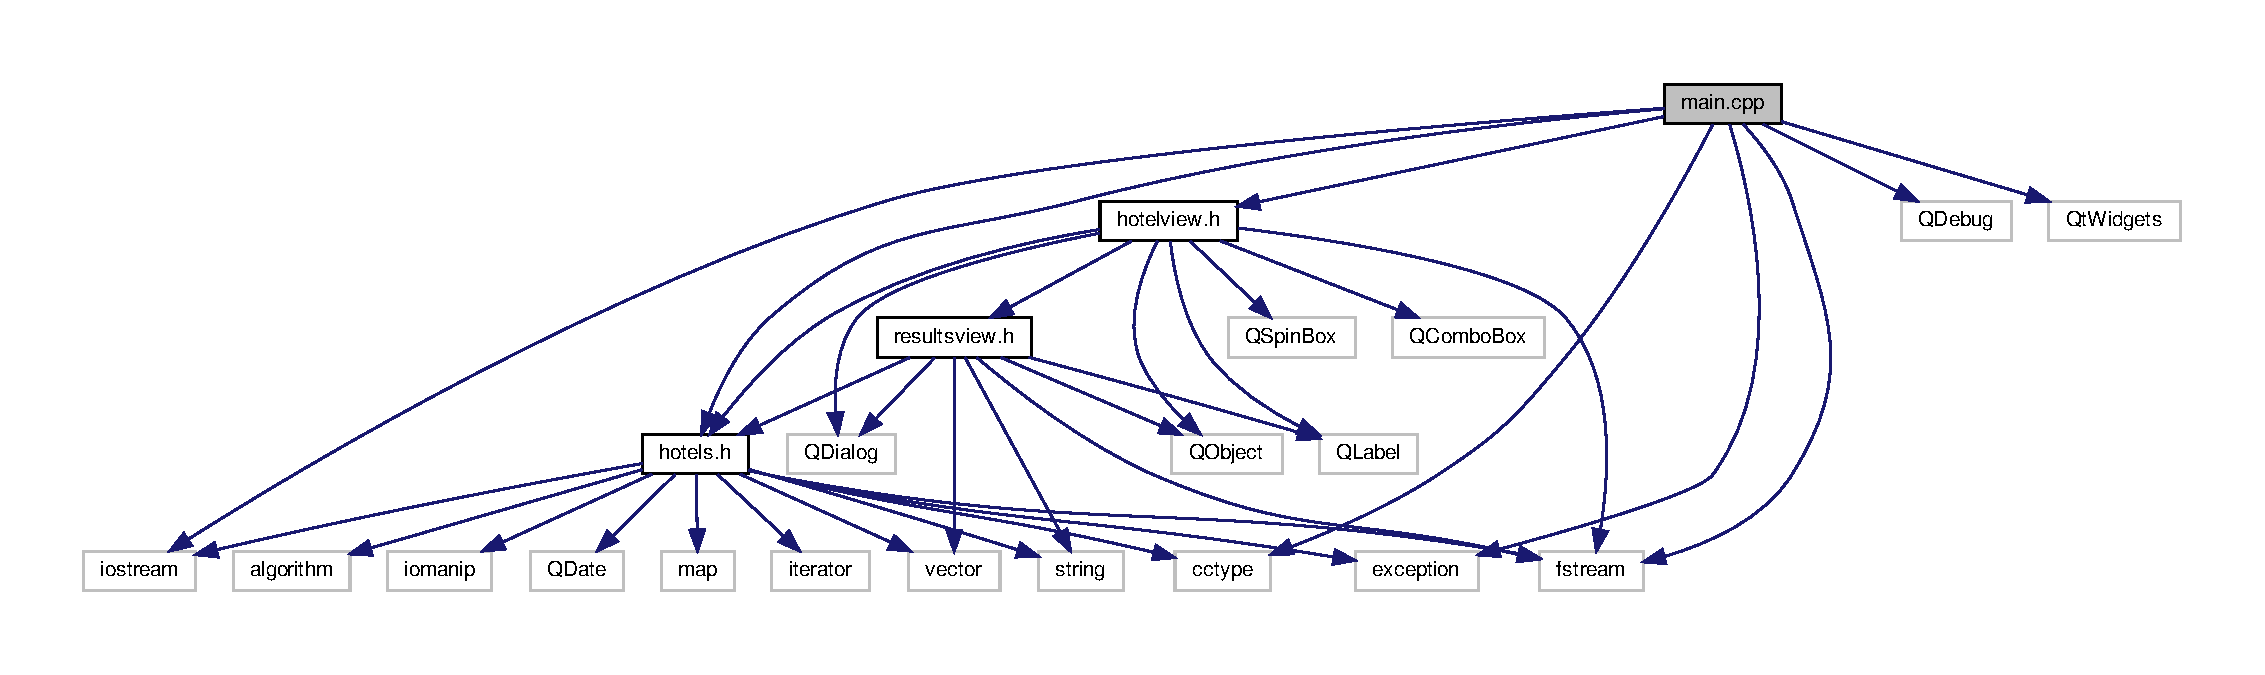
\includegraphics[width=350pt]{main_8cpp__incl}
\end{center}
\end{figure}
\subsection*{Functions}
\begin{DoxyCompactItemize}
\item 
int \hyperlink{main_8cpp_a0ddf1224851353fc92bfbff6f499fa97}{main} (int argc, char $\ast$argv\mbox{[}$\,$\mbox{]})
\end{DoxyCompactItemize}


\subsection{Function Documentation}
\mbox{\Hypertarget{main_8cpp_a0ddf1224851353fc92bfbff6f499fa97}\label{main_8cpp_a0ddf1224851353fc92bfbff6f499fa97}} 
\index{main.\+cpp@{main.\+cpp}!main@{main}}
\index{main@{main}!main.\+cpp@{main.\+cpp}}
\subsubsection{\texorpdfstring{main()}{main()}}
{\footnotesize\ttfamily int main (\begin{DoxyParamCaption}\item[{int}]{argc,  }\item[{char $\ast$}]{argv\mbox{[}$\,$\mbox{]} }\end{DoxyParamCaption})}


\hypertarget{moc__hotel_view_8cpp}{}\section{moc\+\_\+hotelview.\+cpp File Reference}
\label{moc__hotel_view_8cpp}\index{moc\+\_\+hotelview.\+cpp@{moc\+\_\+hotelview.\+cpp}}
{\ttfamily \#include \char`\"{}hotel\+View.\+h\char`\"{}}\newline
{\ttfamily \#include $<$Qt\+Core/qbytearray.\+h$>$}\newline
{\ttfamily \#include $<$Qt\+Core/qmetatype.\+h$>$}\newline
Include dependency graph for moc\+\_\+hotelview.\+cpp\+:\nopagebreak
\begin{figure}[H]
\begin{center}
\leavevmode
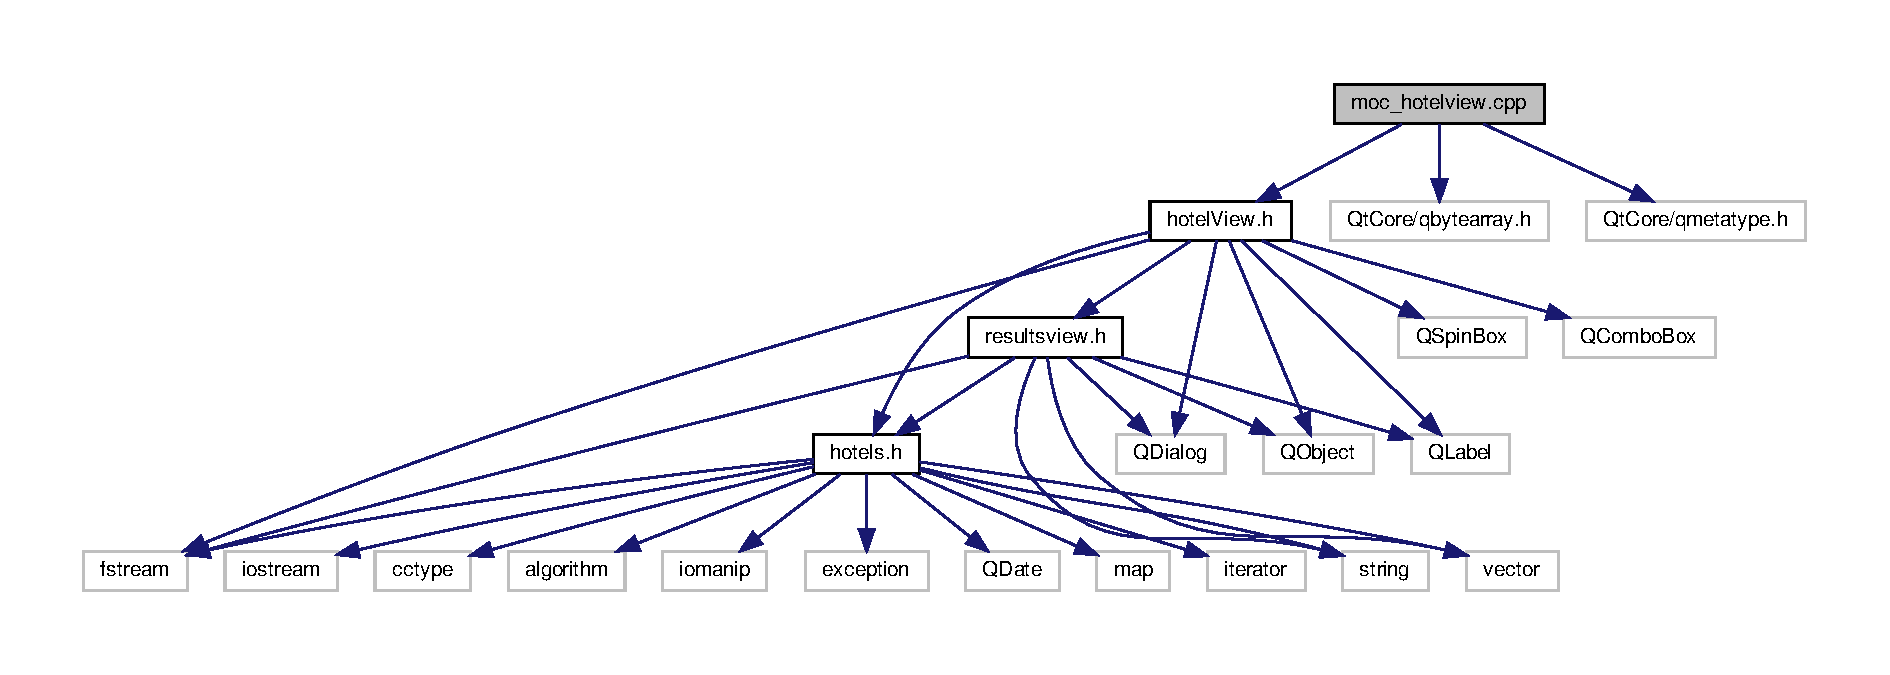
\includegraphics[width=350pt]{moc__hotel_view_8cpp__incl}
\end{center}
\end{figure}
\subsection*{Classes}
\begin{DoxyCompactItemize}
\item 
struct \hyperlink{structqt__meta__stringdata___hotel_view__t}{qt\+\_\+meta\+\_\+stringdata\+\_\+\+Hotel\+View\+\_\+t}
\item 
struct \hyperlink{structqt__meta__stringdata___hotel_view__t}{qt\+\_\+meta\+\_\+stringdata\+\_\+\+Hotel\+View\+\_\+t}
\end{DoxyCompactItemize}
\subsection*{Macros}
\begin{DoxyCompactItemize}
\item 
\#define \hyperlink{moc__hotel_view_8cpp_a75bb9482d242cde0a06c9dbdc6b83abe}{Q\+T\+\_\+\+M\+O\+C\+\_\+\+L\+I\+T\+E\+R\+AL}(idx,  ofs,  len)
\item 
\#define \hyperlink{moc__hotel_view_8cpp_a75bb9482d242cde0a06c9dbdc6b83abe}{Q\+T\+\_\+\+M\+O\+C\+\_\+\+L\+I\+T\+E\+R\+AL}(idx,  ofs,  len)
\end{DoxyCompactItemize}


\subsection{Macro Definition Documentation}
\mbox{\Hypertarget{moc__hotel_view_8cpp_a75bb9482d242cde0a06c9dbdc6b83abe}\label{moc__hotel_view_8cpp_a75bb9482d242cde0a06c9dbdc6b83abe}} 
\index{moc\+\_\+hotel\+View.\+cpp@{moc\+\_\+hotel\+View.\+cpp}!Q\+T\+\_\+\+M\+O\+C\+\_\+\+L\+I\+T\+E\+R\+AL@{Q\+T\+\_\+\+M\+O\+C\+\_\+\+L\+I\+T\+E\+R\+AL}}
\index{Q\+T\+\_\+\+M\+O\+C\+\_\+\+L\+I\+T\+E\+R\+AL@{Q\+T\+\_\+\+M\+O\+C\+\_\+\+L\+I\+T\+E\+R\+AL}!moc\+\_\+hotel\+View.\+cpp@{moc\+\_\+hotel\+View.\+cpp}}
\subsubsection{\texorpdfstring{Q\+T\+\_\+\+M\+O\+C\+\_\+\+L\+I\+T\+E\+R\+AL}{QT\_MOC\_LITERAL}\hspace{0.1cm}{\footnotesize\ttfamily [1/2]}}
{\footnotesize\ttfamily \#define Q\+T\+\_\+\+M\+O\+C\+\_\+\+L\+I\+T\+E\+R\+AL(\begin{DoxyParamCaption}\item[{}]{idx,  }\item[{}]{ofs,  }\item[{}]{len }\end{DoxyParamCaption})}

{\bfseries Value\+:}
\begin{DoxyCode}
Q\_STATIC\_BYTE\_ARRAY\_DATA\_HEADER\_INITIALIZER\_WITH\_OFFSET(len, \(\backslash\)
    qptrdiff(offsetof(\hyperlink{structqt__meta__stringdata___hotel_view__t}{qt\_meta\_stringdata\_HotelView\_t}, stringdata0) + ofs \(\backslash\)
        - idx * \textcolor{keyword}{sizeof}(QByteArrayData)) \(\backslash\)
    )
\end{DoxyCode}
\mbox{\Hypertarget{moc__hotel_view_8cpp_a75bb9482d242cde0a06c9dbdc6b83abe}\label{moc__hotel_view_8cpp_a75bb9482d242cde0a06c9dbdc6b83abe}} 
\index{moc\+\_\+hotel\+View.\+cpp@{moc\+\_\+hotel\+View.\+cpp}!Q\+T\+\_\+\+M\+O\+C\+\_\+\+L\+I\+T\+E\+R\+AL@{Q\+T\+\_\+\+M\+O\+C\+\_\+\+L\+I\+T\+E\+R\+AL}}
\index{Q\+T\+\_\+\+M\+O\+C\+\_\+\+L\+I\+T\+E\+R\+AL@{Q\+T\+\_\+\+M\+O\+C\+\_\+\+L\+I\+T\+E\+R\+AL}!moc\+\_\+hotel\+View.\+cpp@{moc\+\_\+hotel\+View.\+cpp}}
\subsubsection{\texorpdfstring{Q\+T\+\_\+\+M\+O\+C\+\_\+\+L\+I\+T\+E\+R\+AL}{QT\_MOC\_LITERAL}\hspace{0.1cm}{\footnotesize\ttfamily [2/2]}}
{\footnotesize\ttfamily \#define Q\+T\+\_\+\+M\+O\+C\+\_\+\+L\+I\+T\+E\+R\+AL(\begin{DoxyParamCaption}\item[{}]{idx,  }\item[{}]{ofs,  }\item[{}]{len }\end{DoxyParamCaption})}

{\bfseries Value\+:}
\begin{DoxyCode}
Q\_STATIC\_BYTE\_ARRAY\_DATA\_HEADER\_INITIALIZER\_WITH\_OFFSET(len, \(\backslash\)
    qptrdiff(offsetof(\hyperlink{structqt__meta__stringdata___hotel_view__t}{qt\_meta\_stringdata\_HotelView\_t}, stringdata0) + ofs \(\backslash\)
        - idx * \textcolor{keyword}{sizeof}(QByteArrayData)) \(\backslash\)
    )
\end{DoxyCode}

\hypertarget{moc__hotel_view_8cpp}{}\section{moc\+\_\+hotelview.\+cpp File Reference}
\label{moc__hotel_view_8cpp}\index{moc\+\_\+hotelview.\+cpp@{moc\+\_\+hotelview.\+cpp}}
{\ttfamily \#include \char`\"{}hotel\+View.\+h\char`\"{}}\newline
{\ttfamily \#include $<$Qt\+Core/qbytearray.\+h$>$}\newline
{\ttfamily \#include $<$Qt\+Core/qmetatype.\+h$>$}\newline
Include dependency graph for moc\+\_\+hotelview.\+cpp\+:\nopagebreak
\begin{figure}[H]
\begin{center}
\leavevmode
\includegraphics[width=350pt]{moc__hotel_view_8cpp__incl}
\end{center}
\end{figure}
\subsection*{Classes}
\begin{DoxyCompactItemize}
\item 
struct \hyperlink{structqt__meta__stringdata___hotel_view__t}{qt\+\_\+meta\+\_\+stringdata\+\_\+\+Hotel\+View\+\_\+t}
\item 
struct \hyperlink{structqt__meta__stringdata___hotel_view__t}{qt\+\_\+meta\+\_\+stringdata\+\_\+\+Hotel\+View\+\_\+t}
\end{DoxyCompactItemize}
\subsection*{Macros}
\begin{DoxyCompactItemize}
\item 
\#define \hyperlink{moc__hotel_view_8cpp_a75bb9482d242cde0a06c9dbdc6b83abe}{Q\+T\+\_\+\+M\+O\+C\+\_\+\+L\+I\+T\+E\+R\+AL}(idx,  ofs,  len)
\item 
\#define \hyperlink{moc__hotel_view_8cpp_a75bb9482d242cde0a06c9dbdc6b83abe}{Q\+T\+\_\+\+M\+O\+C\+\_\+\+L\+I\+T\+E\+R\+AL}(idx,  ofs,  len)
\end{DoxyCompactItemize}


\subsection{Macro Definition Documentation}
\mbox{\Hypertarget{moc__hotel_view_8cpp_a75bb9482d242cde0a06c9dbdc6b83abe}\label{moc__hotel_view_8cpp_a75bb9482d242cde0a06c9dbdc6b83abe}} 
\index{moc\+\_\+hotel\+View.\+cpp@{moc\+\_\+hotel\+View.\+cpp}!Q\+T\+\_\+\+M\+O\+C\+\_\+\+L\+I\+T\+E\+R\+AL@{Q\+T\+\_\+\+M\+O\+C\+\_\+\+L\+I\+T\+E\+R\+AL}}
\index{Q\+T\+\_\+\+M\+O\+C\+\_\+\+L\+I\+T\+E\+R\+AL@{Q\+T\+\_\+\+M\+O\+C\+\_\+\+L\+I\+T\+E\+R\+AL}!moc\+\_\+hotel\+View.\+cpp@{moc\+\_\+hotel\+View.\+cpp}}
\subsubsection{\texorpdfstring{Q\+T\+\_\+\+M\+O\+C\+\_\+\+L\+I\+T\+E\+R\+AL}{QT\_MOC\_LITERAL}\hspace{0.1cm}{\footnotesize\ttfamily [1/2]}}
{\footnotesize\ttfamily \#define Q\+T\+\_\+\+M\+O\+C\+\_\+\+L\+I\+T\+E\+R\+AL(\begin{DoxyParamCaption}\item[{}]{idx,  }\item[{}]{ofs,  }\item[{}]{len }\end{DoxyParamCaption})}

{\bfseries Value\+:}
\begin{DoxyCode}
Q\_STATIC\_BYTE\_ARRAY\_DATA\_HEADER\_INITIALIZER\_WITH\_OFFSET(len, \(\backslash\)
    qptrdiff(offsetof(\hyperlink{structqt__meta__stringdata___hotel_view__t}{qt\_meta\_stringdata\_HotelView\_t}, stringdata0) + ofs \(\backslash\)
        - idx * \textcolor{keyword}{sizeof}(QByteArrayData)) \(\backslash\)
    )
\end{DoxyCode}
\mbox{\Hypertarget{moc__hotel_view_8cpp_a75bb9482d242cde0a06c9dbdc6b83abe}\label{moc__hotel_view_8cpp_a75bb9482d242cde0a06c9dbdc6b83abe}} 
\index{moc\+\_\+hotel\+View.\+cpp@{moc\+\_\+hotel\+View.\+cpp}!Q\+T\+\_\+\+M\+O\+C\+\_\+\+L\+I\+T\+E\+R\+AL@{Q\+T\+\_\+\+M\+O\+C\+\_\+\+L\+I\+T\+E\+R\+AL}}
\index{Q\+T\+\_\+\+M\+O\+C\+\_\+\+L\+I\+T\+E\+R\+AL@{Q\+T\+\_\+\+M\+O\+C\+\_\+\+L\+I\+T\+E\+R\+AL}!moc\+\_\+hotel\+View.\+cpp@{moc\+\_\+hotel\+View.\+cpp}}
\subsubsection{\texorpdfstring{Q\+T\+\_\+\+M\+O\+C\+\_\+\+L\+I\+T\+E\+R\+AL}{QT\_MOC\_LITERAL}\hspace{0.1cm}{\footnotesize\ttfamily [2/2]}}
{\footnotesize\ttfamily \#define Q\+T\+\_\+\+M\+O\+C\+\_\+\+L\+I\+T\+E\+R\+AL(\begin{DoxyParamCaption}\item[{}]{idx,  }\item[{}]{ofs,  }\item[{}]{len }\end{DoxyParamCaption})}

{\bfseries Value\+:}
\begin{DoxyCode}
Q\_STATIC\_BYTE\_ARRAY\_DATA\_HEADER\_INITIALIZER\_WITH\_OFFSET(len, \(\backslash\)
    qptrdiff(offsetof(\hyperlink{structqt__meta__stringdata___hotel_view__t}{qt\_meta\_stringdata\_HotelView\_t}, stringdata0) + ofs \(\backslash\)
        - idx * \textcolor{keyword}{sizeof}(QByteArrayData)) \(\backslash\)
    )
\end{DoxyCode}

\hypertarget{moc__predefs_8h}{}\section{moc\+\_\+predefs.\+h File Reference}
\label{moc__predefs_8h}\index{moc\+\_\+predefs.\+h@{moc\+\_\+predefs.\+h}}
\subsection*{Macros}
\begin{DoxyCompactItemize}
\item 
\#define \hyperlink{moc__predefs_8h_ac7368721a5741c75d58bc978c47bf1df}{\+\_\+\+\_\+\+S\+S\+P\+\_\+\+S\+T\+R\+O\+N\+G\+\_\+\+\_\+}~3
\item 
\#define \hyperlink{moc__predefs_8h_a63d6f5d1c3371192fe03b3fb06e82400}{\+\_\+\+\_\+\+D\+B\+L\+\_\+\+M\+I\+N\+\_\+\+E\+X\+P\+\_\+\+\_\+}~(-\/1021)
\item 
\#define \hyperlink{moc__predefs_8h_a6605c8368985e3b1885a84d1d44ff798}{\+\_\+\+\_\+\+F\+L\+T32\+X\+\_\+\+M\+A\+X\+\_\+\+E\+X\+P\+\_\+\+\_\+}~1024
\item 
\#define \hyperlink{moc__predefs_8h_ac47e77d27e7d30f01cde452a9cd218ed}{\+\_\+\+\_\+cpp\+\_\+attributes}~200809
\item 
\#define \hyperlink{moc__predefs_8h_a6a762b969d5eea9e6a8db715a5f5a1a9}{\+\_\+\+\_\+\+U\+I\+N\+T\+\_\+\+L\+E\+A\+S\+T16\+\_\+\+M\+A\+X\+\_\+\+\_\+}~0xffff
\item 
\#define \hyperlink{moc__predefs_8h_a72e3c30a05bd2bb63d76550e451a438e}{\+\_\+\+\_\+\+A\+T\+O\+M\+I\+C\+\_\+\+A\+C\+Q\+U\+I\+RE}~2
\item 
\#define \hyperlink{moc__predefs_8h_af071b48310b9018035302c28cfd0424e}{\+\_\+\+\_\+\+F\+L\+T128\+\_\+\+M\+A\+X\+\_\+10\+\_\+\+E\+X\+P\+\_\+\+\_\+}~4932
\item 
\#define \hyperlink{moc__predefs_8h_a6e947aa0a2cb4808d560339fef0d4793}{\+\_\+\+\_\+\+F\+L\+T\+\_\+\+M\+I\+N\+\_\+\+\_\+}~1.\+17549435082228750796873653722224568e-\/38F
\item 
\#define \hyperlink{moc__predefs_8h_a779a207685ad2b8ca4cdab02ece517eb}{\+\_\+\+\_\+\+G\+C\+C\+\_\+\+I\+E\+C\+\_\+559\+\_\+\+C\+O\+M\+P\+L\+EX}~2
\item 
\#define \hyperlink{moc__predefs_8h_ab9bf5af329c2a3a3dc5874289dda6f82}{\+\_\+\+\_\+cpp\+\_\+aggregate\+\_\+nsdmi}~201304
\item 
\#define \hyperlink{moc__predefs_8h_a5a8c0a31337df765b55c6260ef58e51e}{\+\_\+\+\_\+\+U\+I\+N\+T\+\_\+\+L\+E\+A\+S\+T8\+\_\+\+T\+Y\+P\+E\+\_\+\+\_\+}~unsigned char
\item 
\#define \hyperlink{moc__predefs_8h_acb072d4167167be73828de722a2def0b}{\+\_\+\+\_\+\+S\+I\+Z\+E\+O\+F\+\_\+\+F\+L\+O\+A\+T80\+\_\+\+\_\+}~16
\item 
\#define \hyperlink{moc__predefs_8h_adb0d09cff489746c5456407aa832fced}{\+\_\+\+\_\+\+I\+N\+T\+M\+A\+X\+\_\+C}(c)~c \#\# L
\item 
\#define \hyperlink{moc__predefs_8h_ab35e271dce6e7e2190d60b5905375419}{\+\_\+\+\_\+\+C\+H\+A\+R\+\_\+\+B\+I\+T\+\_\+\+\_\+}~8
\item 
\#define \hyperlink{moc__predefs_8h_afd12ac7489bdbbed7fa3cc51023b8f73}{\+\_\+\+\_\+\+U\+I\+N\+T8\+\_\+\+M\+A\+X\+\_\+\+\_\+}~0xff
\item 
\#define \hyperlink{moc__predefs_8h_a8925e15bce319fa2f42c659f6a3e0199}{\+\_\+\+\_\+\+W\+I\+N\+T\+\_\+\+M\+A\+X\+\_\+\+\_\+}~0xffffffffU
\item 
\#define \hyperlink{moc__predefs_8h_a300c6970bb64b04e45a9c2ed139ecce8}{\+\_\+\+\_\+\+F\+L\+T32\+\_\+\+M\+I\+N\+\_\+\+E\+X\+P\+\_\+\+\_\+}~(-\/125)
\item 
\#define \hyperlink{moc__predefs_8h_a60c56e472a1144b03053a2c7a2abb7fb}{\+\_\+\+\_\+cpp\+\_\+static\+\_\+assert}~200410
\item 
\#define \hyperlink{moc__predefs_8h_a2b695357ce4b46971d54e8e9dfe5724f}{\+\_\+\+\_\+\+O\+R\+D\+E\+R\+\_\+\+L\+I\+T\+T\+L\+E\+\_\+\+E\+N\+D\+I\+A\+N\+\_\+\+\_\+}~1234
\item 
\#define \hyperlink{moc__predefs_8h_a66fbb70a69c9f66830f95a20e46091a6}{\+\_\+\+\_\+\+S\+I\+Z\+E\+\_\+\+M\+A\+X\+\_\+\+\_\+}~0xffffffffffffffff\+UL
\item 
\#define \hyperlink{moc__predefs_8h_a65ac8cd0434319a3a31dc031409c218a}{\+\_\+\+\_\+\+W\+C\+H\+A\+R\+\_\+\+M\+A\+X\+\_\+\+\_\+}~0x7fffffff
\item 
\#define \hyperlink{moc__predefs_8h_a33433eca9e18e14156165252746f4d44}{\+\_\+\+\_\+\+G\+C\+C\+\_\+\+H\+A\+V\+E\+\_\+\+S\+Y\+N\+C\+\_\+\+C\+O\+M\+P\+A\+R\+E\+\_\+\+A\+N\+D\+\_\+\+S\+W\+A\+P\+\_\+1}~1
\item 
\#define \hyperlink{moc__predefs_8h_a7237ce09defceeebe3ba0afc528275ac}{\+\_\+\+\_\+\+G\+C\+C\+\_\+\+H\+A\+V\+E\+\_\+\+S\+Y\+N\+C\+\_\+\+C\+O\+M\+P\+A\+R\+E\+\_\+\+A\+N\+D\+\_\+\+S\+W\+A\+P\+\_\+2}~1
\item 
\#define \hyperlink{moc__predefs_8h_a6310789290c9c5717826b56443ce69ec}{\+\_\+\+\_\+\+G\+C\+C\+\_\+\+H\+A\+V\+E\+\_\+\+S\+Y\+N\+C\+\_\+\+C\+O\+M\+P\+A\+R\+E\+\_\+\+A\+N\+D\+\_\+\+S\+W\+A\+P\+\_\+4}~1
\item 
\#define \hyperlink{moc__predefs_8h_aca2a716d3e84ccffe000390bb2e2fb38}{\+\_\+\+\_\+\+D\+B\+L\+\_\+\+D\+E\+N\+O\+R\+M\+\_\+\+M\+I\+N\+\_\+\+\_\+}~double(4.\+94065645841246544176568792868221372e-\/324\+L)
\item 
\#define \hyperlink{moc__predefs_8h_a86bb5059d696b19082c1aff4ae93a87a}{\+\_\+\+\_\+\+G\+C\+C\+\_\+\+H\+A\+V\+E\+\_\+\+S\+Y\+N\+C\+\_\+\+C\+O\+M\+P\+A\+R\+E\+\_\+\+A\+N\+D\+\_\+\+S\+W\+A\+P\+\_\+8}~1
\item 
\#define \hyperlink{moc__predefs_8h_a403ff8d656461ff5a083fb47f73c7da3}{\+\_\+\+\_\+\+G\+C\+C\+\_\+\+A\+T\+O\+M\+I\+C\+\_\+\+C\+H\+A\+R\+\_\+\+L\+O\+C\+K\+\_\+\+F\+R\+EE}~2
\item 
\#define \hyperlink{moc__predefs_8h_a0a3bd26d0b040f0781a238e4aedd3dbe}{\+\_\+\+\_\+\+G\+C\+C\+\_\+\+I\+E\+C\+\_\+559}~2
\item 
\#define \hyperlink{moc__predefs_8h_a00a9f6ceb42fbe18b789b4c1949c49f2}{\+\_\+\+\_\+\+F\+L\+T32\+X\+\_\+\+D\+E\+C\+I\+M\+A\+L\+\_\+\+D\+I\+G\+\_\+\+\_\+}~17
\item 
\#define \hyperlink{moc__predefs_8h_a737828904768e0ab49acbdb3371d8445}{\+\_\+\+\_\+\+F\+L\+T\+\_\+\+E\+V\+A\+L\+\_\+\+M\+E\+T\+H\+O\+D\+\_\+\+\_\+}~0
\item 
\#define \hyperlink{moc__predefs_8h_aa5be39d362c571d48d6236f0bd58f1fc}{\+\_\+\+\_\+unix\+\_\+\+\_\+}~1
\item 
\#define \hyperlink{moc__predefs_8h_ade9dc15e022182eb0a62a0fd17d18b75}{\+\_\+\+\_\+cpp\+\_\+binary\+\_\+literals}~201304
\item 
\#define \hyperlink{moc__predefs_8h_a8ef55ba782e9d01cb22911f97168d06a}{\+\_\+\+\_\+\+F\+L\+T64\+\_\+\+D\+E\+C\+I\+M\+A\+L\+\_\+\+D\+I\+G\+\_\+\+\_\+}~17
\item 
\#define \hyperlink{moc__predefs_8h_a98e298953067135caf4bc0b8e8e7cd01}{\+\_\+\+\_\+\+G\+C\+C\+\_\+\+A\+T\+O\+M\+I\+C\+\_\+\+C\+H\+A\+R32\+\_\+\+T\+\_\+\+L\+O\+C\+K\+\_\+\+F\+R\+EE}~2
\item 
\#define \hyperlink{moc__predefs_8h_a64b6ba77bbc2cb5db2a19f32e954fcc3}{\+\_\+\+\_\+x86\+\_\+64}~1
\item 
\#define \hyperlink{moc__predefs_8h_a559dd2b0792fc2b0b30ba1dd66ca7cdc}{\+\_\+\+\_\+cpp\+\_\+variadic\+\_\+templates}~200704
\item 
\#define \hyperlink{moc__predefs_8h_a17a1ff08595cf7e0c9d1f162b727ccb6}{\+\_\+\+\_\+\+U\+I\+N\+T\+\_\+\+F\+A\+S\+T64\+\_\+\+M\+A\+X\+\_\+\+\_\+}~0xffffffffffffffff\+UL
\item 
\#define \hyperlink{moc__predefs_8h_ac60fe3845f87fdaf6365a733ede87cfe}{\+\_\+\+\_\+\+S\+I\+G\+\_\+\+A\+T\+O\+M\+I\+C\+\_\+\+T\+Y\+P\+E\+\_\+\+\_\+}~int
\item 
\#define \hyperlink{moc__predefs_8h_a1abd7cf346a460459d7fe1a9d4b5dde9}{\+\_\+\+\_\+\+D\+B\+L\+\_\+\+M\+I\+N\+\_\+10\+\_\+\+E\+X\+P\+\_\+\+\_\+}~(-\/307)
\item 
\#define \hyperlink{moc__predefs_8h_a611d40c375b1972669292fd27bc4afb7}{\+\_\+\+\_\+\+F\+I\+N\+I\+T\+E\+\_\+\+M\+A\+T\+H\+\_\+\+O\+N\+L\+Y\+\_\+\+\_\+}~0
\item 
\#define \hyperlink{moc__predefs_8h_a5f5ce266e768d95b9fd04856e5826aff}{\+\_\+\+\_\+cpp\+\_\+variable\+\_\+templates}~201304
\item 
\#define \hyperlink{moc__predefs_8h_ad149c0565fcf669b23f483e5b7f80dbd}{\+\_\+\+\_\+\+G\+N\+U\+C\+\_\+\+P\+A\+T\+C\+H\+L\+E\+V\+E\+L\+\_\+\+\_\+}~0
\item 
\#define \hyperlink{moc__predefs_8h_ac1175c9478c586edee06d1f788a03b83}{\+\_\+\+\_\+\+F\+L\+T32\+\_\+\+H\+A\+S\+\_\+\+D\+E\+N\+O\+R\+M\+\_\+\+\_\+}~1
\item 
\#define \hyperlink{moc__predefs_8h_a27b5eb7cfda61c7f1baeb4d95f3052bb}{\+\_\+\+\_\+\+U\+I\+N\+T\+\_\+\+F\+A\+S\+T8\+\_\+\+M\+A\+X\+\_\+\+\_\+}~0xff
\item 
\#define \hyperlink{moc__predefs_8h_a1c6886956b05c16006d924f77a868410}{\+\_\+\+\_\+has\+\_\+include}(S\+TR)~\+\_\+\+\_\+has\+\_\+include\+\_\+\+\_\+(S\+TR)
\item 
\#define \hyperlink{moc__predefs_8h_a3d4fe0f0b2e3ae12569d4a663dee8a0c}{\+\_\+\+\_\+\+D\+E\+C64\+\_\+\+M\+A\+X\+\_\+\+E\+X\+P\+\_\+\+\_\+}~385
\item 
\#define \hyperlink{moc__predefs_8h_ad36bc14a0433c9f88496bed4ccbd65a3}{\+\_\+\+\_\+\+I\+N\+T8\+\_\+C}(c)~c
\item 
\#define \hyperlink{moc__predefs_8h_a967b4ada96d28b97bc07e26e1def8e66}{\+\_\+\+\_\+\+I\+N\+T\+\_\+\+L\+E\+A\+S\+T8\+\_\+\+W\+I\+D\+T\+H\+\_\+\+\_\+}~8
\item 
\#define \hyperlink{moc__predefs_8h_a4bf843ffcadf9b162b74c1b7e546e8e9}{\+\_\+\+\_\+\+U\+I\+N\+T\+\_\+\+L\+E\+A\+S\+T64\+\_\+\+M\+A\+X\+\_\+\+\_\+}~0xffffffffffffffff\+UL
\item 
\#define \hyperlink{moc__predefs_8h_a4f69990d03f9fb0c390a6fbad28a737b}{\+\_\+\+\_\+\+S\+H\+R\+T\+\_\+\+M\+A\+X\+\_\+\+\_\+}~0x7fff
\item 
\#define \hyperlink{moc__predefs_8h_a06fd91f0507a4f364e469c8055f4265a}{\+\_\+\+\_\+\+L\+D\+B\+L\+\_\+\+M\+A\+X\+\_\+\+\_\+}~1.\+18973149535723176502126385303097021e+4932L
\item 
\#define \hyperlink{moc__predefs_8h_af707469f32a983b229e6c7e0e4efc063}{\+\_\+\+\_\+\+F\+L\+T64\+X\+\_\+\+M\+A\+X\+\_\+10\+\_\+\+E\+X\+P\+\_\+\+\_\+}~4932
\item 
\#define \hyperlink{moc__predefs_8h_aaf06a1464d33431377a2ee5293ec70d2}{\+\_\+\+\_\+\+U\+I\+N\+T\+\_\+\+L\+E\+A\+S\+T8\+\_\+\+M\+A\+X\+\_\+\+\_\+}~0xff
\item 
\#define \hyperlink{moc__predefs_8h_a9685ff8e617f3c5892c2a6fe3484f3b7}{\+\_\+\+\_\+\+G\+C\+C\+\_\+\+A\+T\+O\+M\+I\+C\+\_\+\+B\+O\+O\+L\+\_\+\+L\+O\+C\+K\+\_\+\+F\+R\+EE}~2
\item 
\#define \hyperlink{moc__predefs_8h_a960cb27a87591af89eddb328647f1534}{\+\_\+\+\_\+\+F\+L\+T128\+\_\+\+D\+E\+N\+O\+R\+M\+\_\+\+M\+I\+N\+\_\+\+\_\+}~6.\+47517511943802511092443895822764655e-\/4966\+F128
\item 
\#define \hyperlink{moc__predefs_8h_ab86380373ae9fa385c8a2464023774a8}{\+\_\+\+\_\+\+U\+I\+N\+T\+M\+A\+X\+\_\+\+T\+Y\+P\+E\+\_\+\+\_\+}~long unsigned int
\item 
\#define \hyperlink{moc__predefs_8h_a6c6342c53a7213211680dc5caae14491}{\+\_\+\+\_\+linux}~1
\item 
\#define \hyperlink{moc__predefs_8h_a13526b223391d4982c4c172c29bfdc1e}{\+\_\+\+\_\+\+D\+E\+C32\+\_\+\+E\+P\+S\+I\+L\+O\+N\+\_\+\+\_\+}~1\+E-\/6\+DF
\item 
\#define \hyperlink{moc__predefs_8h_af635b5d104ef9858a68ab2c56677fd2d}{\+\_\+\+\_\+\+F\+L\+T\+\_\+\+E\+V\+A\+L\+\_\+\+M\+E\+T\+H\+O\+D\+\_\+\+T\+S\+\_\+18661\+\_\+3\+\_\+\+\_\+}~0
\item 
\#define \hyperlink{moc__predefs_8h_ac3cd8b035cfb8a68f6d1119ace36f1cc}{\+\_\+\+\_\+unix}~1
\item 
\#define \hyperlink{moc__predefs_8h_ab4425dccbcddb2363a2a8a67367a5b42}{\+\_\+\+\_\+\+U\+I\+N\+T32\+\_\+\+M\+A\+X\+\_\+\+\_\+}~0xffffffffU
\item 
\#define \hyperlink{moc__predefs_8h_a213133a8dca206becf88c2e3523b124a}{\+\_\+\+\_\+\+G\+X\+X\+\_\+\+E\+X\+P\+E\+R\+I\+M\+E\+N\+T\+A\+L\+\_\+\+C\+X\+X0\+X\+\_\+\+\_\+}~1
\item 
\#define \hyperlink{moc__predefs_8h_ae221a8e373285cf10c22926762f477f5}{\+\_\+\+\_\+\+L\+D\+B\+L\+\_\+\+M\+A\+X\+\_\+\+E\+X\+P\+\_\+\+\_\+}~16384
\item 
\#define \hyperlink{moc__predefs_8h_aad2e8f7e8d06ab966a1210f4a7d65770}{\+\_\+\+\_\+\+F\+L\+T128\+\_\+\+M\+I\+N\+\_\+\+E\+X\+P\+\_\+\+\_\+}~(-\/16381)
\item 
\#define \hyperlink{moc__predefs_8h_a135696718aa5b38e58be73aaece6654f}{\+\_\+\+\_\+\+W\+I\+N\+T\+\_\+\+M\+I\+N\+\_\+\+\_\+}~0U
\item 
\#define \hyperlink{moc__predefs_8h_a1b27e3508a4c1e97875297882a95f503}{\+\_\+\+\_\+linux\+\_\+\+\_\+}~1
\item 
\#define \hyperlink{moc__predefs_8h_a784d5a4b7494076d83772a819916b039}{\+\_\+\+\_\+\+F\+L\+T128\+\_\+\+M\+I\+N\+\_\+10\+\_\+\+E\+X\+P\+\_\+\+\_\+}~(-\/4931)
\item 
\#define \hyperlink{moc__predefs_8h_a6091ba87f9a538a9685b7997a64a64db}{\+\_\+\+\_\+\+I\+N\+T\+\_\+\+L\+E\+A\+S\+T16\+\_\+\+W\+I\+D\+T\+H\+\_\+\+\_\+}~16
\item 
\#define \hyperlink{moc__predefs_8h_a87b7ceac2198cab045e40c9a64b11679}{\+\_\+\+\_\+\+S\+C\+H\+A\+R\+\_\+\+M\+A\+X\+\_\+\+\_\+}~0x7f
\item 
\#define \hyperlink{moc__predefs_8h_a39e5016b6c2adbc3a6b1674c458d4dc5}{\+\_\+\+\_\+\+F\+L\+T128\+\_\+\+M\+A\+N\+T\+\_\+\+D\+I\+G\+\_\+\+\_\+}~113
\item 
\#define \hyperlink{moc__predefs_8h_a01b915d3ec5439de746f1d5e9f76dc3d}{\+\_\+\+\_\+\+W\+C\+H\+A\+R\+\_\+\+M\+I\+N\+\_\+\+\_\+}~(-\/\hyperlink{moc__predefs_8h_a65ac8cd0434319a3a31dc031409c218a}{\+\_\+\+\_\+\+W\+C\+H\+A\+R\+\_\+\+M\+A\+X\+\_\+\+\_\+} -\/ 1)
\item 
\#define \hyperlink{moc__predefs_8h_a4b8971e411b88166747d2a3c2425eaee}{\+\_\+\+\_\+\+I\+N\+T64\+\_\+C}(c)~c \#\# L
\item 
\#define \hyperlink{moc__predefs_8h_a61969667ef3b668024a20df9bc34c991}{\+\_\+\+\_\+\+D\+B\+L\+\_\+\+D\+I\+G\+\_\+\+\_\+}~15
\item 
\#define \hyperlink{moc__predefs_8h_aa808bc3159395526ac0c07d36b87dec1}{\+\_\+\+\_\+\+G\+C\+C\+\_\+\+A\+T\+O\+M\+I\+C\+\_\+\+P\+O\+I\+N\+T\+E\+R\+\_\+\+L\+O\+C\+K\+\_\+\+F\+R\+EE}~2
\item 
\#define \hyperlink{moc__predefs_8h_ac070fafc444399b9243e0366b4ce4ef7}{\+\_\+\+\_\+\+F\+L\+T64\+X\+\_\+\+M\+A\+N\+T\+\_\+\+D\+I\+G\+\_\+\+\_\+}~64
\item 
\#define \hyperlink{moc__predefs_8h_a4b2be09502f3fe1cd13838c6761803b3}{\+\_\+\+\_\+\+S\+I\+Z\+E\+O\+F\+\_\+\+I\+N\+T\+\_\+\+\_\+}~4
\item 
\#define \hyperlink{moc__predefs_8h_a8bd657ce95940b7c6087cf5aa54d5280}{\+\_\+\+\_\+\+S\+I\+Z\+E\+O\+F\+\_\+\+P\+O\+I\+N\+T\+E\+R\+\_\+\+\_\+}~8
\item 
\#define \hyperlink{moc__predefs_8h_a7f18358ae5a65523140cb561bbeaa3a9}{\+\_\+\+\_\+\+G\+C\+C\+\_\+\+A\+T\+O\+M\+I\+C\+\_\+\+C\+H\+A\+R16\+\_\+\+T\+\_\+\+L\+O\+C\+K\+\_\+\+F\+R\+EE}~2
\item 
\#define \hyperlink{moc__predefs_8h_aff6bf0ff0fa3b5cbd23a8ae1131c87a9}{\+\_\+\+\_\+\+U\+S\+E\+R\+\_\+\+L\+A\+B\+E\+L\+\_\+\+P\+R\+E\+F\+I\+X\+\_\+\+\_\+}
\item 
\#define \hyperlink{moc__predefs_8h_a098c7fe44eed71241990da5db8f99bc3}{\+\_\+\+\_\+\+F\+L\+T64\+X\+\_\+\+E\+P\+S\+I\+L\+O\+N\+\_\+\+\_\+}~1.\+08420217248550443400745280086994171e-\/19\+F64x
\item 
\#define \hyperlink{moc__predefs_8h_a309fa84aefd09132258bbe21c20ef7d4}{\+\_\+\+\_\+\+S\+T\+D\+C\+\_\+\+H\+O\+S\+T\+E\+D\+\_\+\+\_\+}~1
\item 
\#define \hyperlink{moc__predefs_8h_a87140cc80075e8907e7bbfd910c5642a}{\+\_\+\+\_\+\+L\+D\+B\+L\+\_\+\+H\+A\+S\+\_\+\+I\+N\+F\+I\+N\+I\+T\+Y\+\_\+\+\_\+}~1
\item 
\#define \hyperlink{moc__predefs_8h_aa021702c3b7627dccaa51c33a2c5a8d1}{\+\_\+\+\_\+\+F\+L\+T32\+\_\+\+D\+I\+G\+\_\+\+\_\+}~6
\item 
\#define \hyperlink{moc__predefs_8h_a7ac5a3b1dc00b508a391f8c6c37e2165}{\+\_\+\+\_\+\+F\+L\+T\+\_\+\+E\+P\+S\+I\+L\+O\+N\+\_\+\+\_\+}~1.\+19209289550781250000000000000000000e-\/7F
\item 
\#define \hyperlink{moc__predefs_8h_afb5a2a4891df4551832357e97c6c3c59}{\+\_\+\+\_\+\+G\+X\+X\+\_\+\+W\+E\+A\+K\+\_\+\+\_\+}~1
\item 
\#define \hyperlink{moc__predefs_8h_aeb2d8312284d49b1e44c7d003bd8b54b}{\+\_\+\+\_\+\+S\+H\+R\+T\+\_\+\+W\+I\+D\+T\+H\+\_\+\+\_\+}~16
\item 
\#define \hyperlink{moc__predefs_8h_ab572f59c4b0c5a1f4c2953f38a76d7b3}{\+\_\+\+\_\+\+L\+D\+B\+L\+\_\+\+M\+I\+N\+\_\+\+\_\+}~3.\+36210314311209350626267781732175260e-\/4932L
\item 
\#define \hyperlink{moc__predefs_8h_ad3165a97a460b88ccdea80967918f250}{\+\_\+\+\_\+\+D\+E\+C32\+\_\+\+M\+A\+X\+\_\+\+\_\+}~9.\+999999\+E96\+DF
\item 
\#define \hyperlink{moc__predefs_8h_aaa322b38474911c60e45134194bd6e8f}{\+\_\+\+\_\+cpp\+\_\+threadsafe\+\_\+static\+\_\+init}~200806
\item 
\#define \hyperlink{moc__predefs_8h_ac0fe3e739d0b847c07dde20eabf2ab3d}{\+\_\+\+\_\+\+F\+L\+T64\+X\+\_\+\+D\+E\+N\+O\+R\+M\+\_\+\+M\+I\+N\+\_\+\+\_\+}~3.\+64519953188247460252840593361941982e-\/4951\+F64x
\item 
\#define \hyperlink{moc__predefs_8h_a8f246ad899706f78b8dfcd33daff7b07}{\+\_\+\+\_\+\+F\+L\+T32\+X\+\_\+\+H\+A\+S\+\_\+\+I\+N\+F\+I\+N\+I\+T\+Y\+\_\+\+\_\+}~1
\item 
\#define \hyperlink{moc__predefs_8h_abf681096fa9e21512a3fe83f0dcfdb36}{\+\_\+\+\_\+\+I\+N\+T32\+\_\+\+M\+A\+X\+\_\+\+\_\+}~0x7fffffff
\item 
\#define \hyperlink{moc__predefs_8h_ad3907b8d9bb2265255e6e0d66d91d165}{\+\_\+\+\_\+\+I\+N\+T\+\_\+\+W\+I\+D\+T\+H\+\_\+\+\_\+}~32
\item 
\#define \hyperlink{moc__predefs_8h_aaa8084a56e3732008acafea8fd15eb2f}{\+\_\+\+\_\+\+S\+I\+Z\+E\+O\+F\+\_\+\+L\+O\+N\+G\+\_\+\+\_\+}~8
\item 
\#define \hyperlink{moc__predefs_8h_ab7d84ba8d87b8bb40aa752334bb51b23}{\+\_\+\+\_\+\+S\+T\+D\+C\+\_\+\+I\+E\+C\+\_\+559\+\_\+\+\_\+}~1
\item 
\#define \hyperlink{moc__predefs_8h_acb6063ed9d8841cf71c93f2bf34832e0}{\+\_\+\+\_\+\+S\+T\+D\+C\+\_\+\+I\+S\+O\+\_\+10646\+\_\+\+\_\+}~201706L
\item 
\#define \hyperlink{moc__predefs_8h_aa860a111dcff819d3502dda14f8ac778}{\+\_\+\+\_\+\+U\+I\+N\+T16\+\_\+C}(c)~c
\item 
\#define \hyperlink{moc__predefs_8h_a96b511bfa61e4203ec3668fb39063309}{\+\_\+\+\_\+\+P\+T\+R\+D\+I\+F\+F\+\_\+\+W\+I\+D\+T\+H\+\_\+\+\_\+}~64
\item 
\#define \hyperlink{moc__predefs_8h_aeb56455e98000942147dfd63ec1c2fa6}{\+\_\+\+\_\+\+D\+E\+C\+I\+M\+A\+L\+\_\+\+D\+I\+G\+\_\+\+\_\+}~21
\item 
\#define \hyperlink{moc__predefs_8h_ad293ff29c0ac9a6b4187d366d6de3772}{\+\_\+\+\_\+\+F\+L\+T64\+\_\+\+E\+P\+S\+I\+L\+O\+N\+\_\+\+\_\+}~2.\+22044604925031308084726333618164062e-\/16\+F64
\item 
\#define \hyperlink{moc__predefs_8h_a51b087854dc3c2f76946efb432745639}{\+\_\+\+\_\+gnu\+\_\+linux\+\_\+\+\_\+}~1
\item 
\#define \hyperlink{moc__predefs_8h_a4e8a5398566f8b2666a8a71b2dbcf3ca}{\+\_\+\+\_\+\+I\+N\+T\+M\+A\+X\+\_\+\+W\+I\+D\+T\+H\+\_\+\+\_\+}~64
\item 
\#define \hyperlink{moc__predefs_8h_aceda5e62622b9783846d26610d038f71}{\+\_\+\+\_\+\+F\+L\+T64\+\_\+\+M\+I\+N\+\_\+\+E\+X\+P\+\_\+\+\_\+}~(-\/1021)
\item 
\#define \hyperlink{moc__predefs_8h_a370369ba2463363de726ff9394861a2b}{\+\_\+\+\_\+has\+\_\+include\+\_\+next}(S\+TR)~\+\_\+\+\_\+has\+\_\+include\+\_\+next\+\_\+\+\_\+(S\+TR)
\item 
\#define \hyperlink{moc__predefs_8h_ad2396317be1036fdc4481d54343487de}{\+\_\+\+\_\+\+F\+L\+T64\+X\+\_\+\+M\+I\+N\+\_\+10\+\_\+\+E\+X\+P\+\_\+\+\_\+}~(-\/4931)
\item 
\#define \hyperlink{moc__predefs_8h_a10a15ae17c3b791fe9b9721965ebfee4}{\+\_\+\+\_\+\+L\+D\+B\+L\+\_\+\+H\+A\+S\+\_\+\+Q\+U\+I\+E\+T\+\_\+\+N\+A\+N\+\_\+\+\_\+}~1
\item 
\#define \hyperlink{moc__predefs_8h_a6c163c6e58545740cbae55ad8ffa027f}{\+\_\+\+\_\+\+F\+L\+T64\+\_\+\+M\+A\+N\+T\+\_\+\+D\+I\+G\+\_\+\+\_\+}~53
\item 
\#define \hyperlink{moc__predefs_8h_aa51016843ec55a0a9df7ce9f85767ee7}{\+\_\+\+\_\+\+G\+N\+U\+C\+\_\+\+\_\+}~7
\item 
\#define \hyperlink{moc__predefs_8h_af607715c8c9a98aa72c81c6629554b0d}{\+\_\+\+\_\+\+G\+X\+X\+\_\+\+R\+T\+TI}~1
\item 
\#define \hyperlink{moc__predefs_8h_a4b376612fb6ea83330a589449279da42}{\+\_\+\+\_\+pie\+\_\+\+\_\+}~2
\item 
\#define \hyperlink{moc__predefs_8h_ab61dd6e368adb90e2eff5739188b0bcb}{\+\_\+\+\_\+\+M\+M\+X\+\_\+\+\_\+}~1
\item 
\#define \hyperlink{moc__predefs_8h_a9e077def8c310cdb5fef37666a92c5a5}{\+\_\+\+\_\+cpp\+\_\+delegating\+\_\+constructors}~200604
\item 
\#define \hyperlink{moc__predefs_8h_a82a2c3ff271d1685b450975ffa68544a}{\+\_\+\+\_\+\+F\+L\+T\+\_\+\+H\+A\+S\+\_\+\+D\+E\+N\+O\+R\+M\+\_\+\+\_\+}~1
\item 
\#define \hyperlink{moc__predefs_8h_aae92712264b830cd7d24d4b81d502ffb}{\+\_\+\+\_\+\+S\+I\+Z\+E\+O\+F\+\_\+\+L\+O\+N\+G\+\_\+\+D\+O\+U\+B\+L\+E\+\_\+\+\_\+}~16
\item 
\#define \hyperlink{moc__predefs_8h_a2c25ec0f0ae74f9d8a7c373288a28dd1}{\+\_\+\+\_\+\+B\+I\+G\+G\+E\+S\+T\+\_\+\+A\+L\+I\+G\+N\+M\+E\+N\+T\+\_\+\+\_\+}~16
\item 
\#define \hyperlink{moc__predefs_8h_a93a5a9d251e5bff3c2a130627f20e782}{\+\_\+\+\_\+\+S\+T\+D\+C\+\_\+\+U\+T\+F\+\_\+16\+\_\+\+\_\+}~1
\item 
\#define \hyperlink{moc__predefs_8h_aeb14f5cf7cca3a01c2f6a0015e981eb1}{\+\_\+\+\_\+\+F\+L\+T64\+\_\+\+M\+A\+X\+\_\+10\+\_\+\+E\+X\+P\+\_\+\+\_\+}~308
\item 
\#define \hyperlink{moc__predefs_8h_a170219070ed7bdfea9f88121c9abbaea}{\+\_\+\+\_\+\+F\+L\+T32\+\_\+\+H\+A\+S\+\_\+\+I\+N\+F\+I\+N\+I\+T\+Y\+\_\+\+\_\+}~1
\item 
\#define \hyperlink{moc__predefs_8h_a711d7b7f27671b10b11a74c37f653ad7}{\+\_\+\+\_\+\+D\+B\+L\+\_\+\+M\+A\+X\+\_\+\+\_\+}~double(1.\+79769313486231570814527423731704357e+308\+L)
\item 
\#define \hyperlink{moc__predefs_8h_a7377e1bc6bd2fd9bcfe98283ab0e9037}{\+\_\+\+\_\+cpp\+\_\+raw\+\_\+strings}~200710
\item 
\#define \hyperlink{moc__predefs_8h_a84479d2bbe1d7286f406fcc302f41376}{\+\_\+\+\_\+\+I\+N\+T\+\_\+\+F\+A\+S\+T32\+\_\+\+M\+A\+X\+\_\+\+\_\+}~0x7fffffffffffffffL
\item 
\#define \hyperlink{moc__predefs_8h_a3dd03066dbb351dfa51353c80a7902a2}{\+\_\+\+\_\+\+D\+B\+L\+\_\+\+H\+A\+S\+\_\+\+I\+N\+F\+I\+N\+I\+T\+Y\+\_\+\+\_\+}~1
\item 
\#define \hyperlink{moc__predefs_8h_aa3f186f612efe5edfcc371c95617f06f}{\+\_\+\+\_\+\+I\+N\+T64\+\_\+\+M\+A\+X\+\_\+\+\_\+}~0x7fffffffffffffffL
\item 
\#define \hyperlink{moc__predefs_8h_a79e289c54a8c9851b2b118d442bbc26c}{\+\_\+\+\_\+\+D\+E\+C32\+\_\+\+M\+I\+N\+\_\+\+E\+X\+P\+\_\+\+\_\+}~(-\/94)
\item 
\#define \hyperlink{moc__predefs_8h_a8394afe92148ddbdf0e0697978cd1382}{\+\_\+\+\_\+\+I\+N\+T\+P\+T\+R\+\_\+\+W\+I\+D\+T\+H\+\_\+\+\_\+}~64
\item 
\#define \hyperlink{moc__predefs_8h_a97163404b3b71f857e35be74607f88f7}{\+\_\+\+\_\+\+F\+L\+T32\+X\+\_\+\+H\+A\+S\+\_\+\+D\+E\+N\+O\+R\+M\+\_\+\+\_\+}~1
\item 
\#define \hyperlink{moc__predefs_8h_a6a4d11835d03027f3929b84fe7b55bf6}{\+\_\+\+\_\+\+I\+N\+T\+\_\+\+F\+A\+S\+T16\+\_\+\+T\+Y\+P\+E\+\_\+\+\_\+}~long int
\item 
\#define \hyperlink{moc__predefs_8h_a3c7f3130e367d47bcc27a0a41278155e}{\+\_\+\+\_\+\+L\+D\+B\+L\+\_\+\+H\+A\+S\+\_\+\+D\+E\+N\+O\+R\+M\+\_\+\+\_\+}~1
\item 
\#define \hyperlink{moc__predefs_8h_a1b391bc7ed92f79666c4a5d840aa1edd}{\+\_\+\+\_\+cplusplus}~201402L
\item 
\#define \hyperlink{moc__predefs_8h_af73192acc2dd2095bd3524ca5ee9dca9}{\+\_\+\+\_\+cpp\+\_\+ref\+\_\+qualifiers}~200710
\item 
\#define \hyperlink{moc__predefs_8h_aaab7817ee2e4bb88b5178e101e7ab2a6}{\+\_\+\+\_\+\+D\+E\+C128\+\_\+\+M\+A\+X\+\_\+\+\_\+}~9.\+999999999999999999999999999999999\+E6144\+DL
\item 
\#define \hyperlink{moc__predefs_8h_a97e13c059a63d2d547cc4a9f386641d2}{\+\_\+\+\_\+\+I\+N\+T\+\_\+\+L\+E\+A\+S\+T32\+\_\+\+M\+A\+X\+\_\+\+\_\+}~0x7fffffff
\item 
\#define \hyperlink{moc__predefs_8h_a1f993b902b5b1dba7d5b043d0abc347b}{\+\_\+\+\_\+\+D\+E\+C32\+\_\+\+M\+I\+N\+\_\+\+\_\+}~1\+E-\/95\+DF
\item 
\#define \hyperlink{moc__predefs_8h_aa806e8f7ce2a8db3bf676735fca2ac51}{\+\_\+\+\_\+\+D\+E\+P\+R\+E\+C\+A\+T\+ED}~1
\item 
\#define \hyperlink{moc__predefs_8h_acfffb302850fa081bd63c30573077004}{\+\_\+\+\_\+cpp\+\_\+rvalue\+\_\+references}~200610
\item 
\#define \hyperlink{moc__predefs_8h_a9a8a7cd9484baf4b72ab15682745d119}{\+\_\+\+\_\+\+D\+B\+L\+\_\+\+M\+A\+X\+\_\+\+E\+X\+P\+\_\+\+\_\+}~1024
\item 
\#define \hyperlink{moc__predefs_8h_aba008af276ac0e3f85d1479af98f62b0}{\+\_\+\+\_\+\+W\+C\+H\+A\+R\+\_\+\+W\+I\+D\+T\+H\+\_\+\+\_\+}~32
\item 
\#define \hyperlink{moc__predefs_8h_a8d44614ef6d7f2bbbd9224d416d867b9}{\+\_\+\+\_\+\+F\+L\+T32\+\_\+\+M\+A\+X\+\_\+\+\_\+}~3.\+40282346638528859811704183484516925e+38\+F32
\item 
\#define \hyperlink{moc__predefs_8h_abd2230e0e187a5bae549a0ba786b311b}{\+\_\+\+\_\+\+D\+E\+C128\+\_\+\+E\+P\+S\+I\+L\+O\+N\+\_\+\+\_\+}~1\+E-\/33\+DL
\item 
\#define \hyperlink{moc__predefs_8h_ad8885a68f76fac734a20349f9b8cac69}{\+\_\+\+\_\+\+S\+S\+E2\+\_\+\+M\+A\+T\+H\+\_\+\+\_\+}~1
\item 
\#define \hyperlink{moc__predefs_8h_a6bb8315e719b7306f47cde3b4b30d91f}{\+\_\+\+\_\+\+A\+T\+O\+M\+I\+C\+\_\+\+H\+L\+E\+\_\+\+R\+E\+L\+E\+A\+SE}~131072
\item 
\#define \hyperlink{moc__predefs_8h_ac29c76a6702808cfc4a5f661d0d33c2c}{\+\_\+\+\_\+\+P\+T\+R\+D\+I\+F\+F\+\_\+\+M\+A\+X\+\_\+\+\_\+}~0x7fffffffffffffffL
\item 
\#define \hyperlink{moc__predefs_8h_ac78e83c300ae463c501bbe70c5a2a8c7}{\+\_\+\+\_\+amd64}~1
\item 
\#define \hyperlink{moc__predefs_8h_a80dc30fae2c51e5db5b4f5eb7400cd1a}{\+\_\+\+\_\+\+S\+T\+D\+C\+\_\+\+N\+O\+\_\+\+T\+H\+R\+E\+A\+D\+S\+\_\+\+\_\+}~1
\item 
\#define \hyperlink{moc__predefs_8h_ac227f24525ec0825a758b2eb0869dc8f}{\+\_\+\+\_\+\+A\+T\+O\+M\+I\+C\+\_\+\+H\+L\+E\+\_\+\+A\+C\+Q\+U\+I\+RE}~65536
\item 
\#define \hyperlink{moc__predefs_8h_a22791bdfea523b20c18eff848609fa9d}{\+\_\+\+\_\+\+F\+L\+T32\+\_\+\+H\+A\+S\+\_\+\+Q\+U\+I\+E\+T\+\_\+\+N\+A\+N\+\_\+\+\_\+}~1
\item 
\#define \hyperlink{moc__predefs_8h_ae7afb460abc6122c6a5f206d78bcae4e}{\+\_\+\+\_\+\+G\+N\+U\+G\+\_\+\+\_\+}~7
\item 
\#define \hyperlink{moc__predefs_8h_a9bed0d0b1893211f857ad76d6728ea7e}{\+\_\+\+\_\+\+L\+O\+N\+G\+\_\+\+L\+O\+N\+G\+\_\+\+M\+A\+X\+\_\+\+\_\+}~0x7fffffffffffffff\+LL
\item 
\#define \hyperlink{moc__predefs_8h_ab6eb3d66486ef05ac7f1d489bfc675b4}{\+\_\+\+\_\+\+S\+I\+Z\+E\+O\+F\+\_\+\+S\+I\+Z\+E\+\_\+\+T\+\_\+\+\_\+}~8
\item 
\#define \hyperlink{moc__predefs_8h_a6e4065bb57fe77e1d8635f8108bf3c64}{\+\_\+\+\_\+cpp\+\_\+rvalue\+\_\+reference}~200610
\item 
\#define \hyperlink{moc__predefs_8h_adeecd09fc579ff3f8222cf8ae581b936}{\+\_\+\+\_\+cpp\+\_\+nsdmi}~200809
\item 
\#define \hyperlink{moc__predefs_8h_a287cbae3fb7eb2bdc8906729897524c9}{\+\_\+\+\_\+\+F\+L\+T64\+X\+\_\+\+M\+I\+N\+\_\+\+E\+X\+P\+\_\+\+\_\+}~(-\/16381)
\item 
\#define \hyperlink{moc__predefs_8h_a808f04c28bb0ef2d6b77dd66564ad351}{\+\_\+\+\_\+\+S\+I\+Z\+E\+O\+F\+\_\+\+W\+I\+N\+T\+\_\+\+T\+\_\+\+\_\+}~4
\item 
\#define \hyperlink{moc__predefs_8h_a895181efde95bdfb3489ba3018c48582}{\+\_\+\+\_\+\+L\+O\+N\+G\+\_\+\+L\+O\+N\+G\+\_\+\+W\+I\+D\+T\+H\+\_\+\+\_\+}~64
\item 
\#define \hyperlink{moc__predefs_8h_a2b46de6050feed05210bef65feef9c42}{\+\_\+\+\_\+cpp\+\_\+initializer\+\_\+lists}~200806
\item 
\#define \hyperlink{moc__predefs_8h_a731bd57ce12918b6118b6a3e37c20d8e}{\+\_\+\+\_\+\+F\+L\+T32\+\_\+\+M\+A\+X\+\_\+\+E\+X\+P\+\_\+\+\_\+}~128
\item 
\#define \hyperlink{moc__predefs_8h_a0958474253d23ca2c87e817c16f74eda}{\+\_\+\+\_\+cpp\+\_\+hex\+\_\+float}~201603
\item 
\#define \hyperlink{moc__predefs_8h_a89cfc45cff96747b74ae03bdb2310814}{\+\_\+\+\_\+\+G\+C\+C\+\_\+\+H\+A\+V\+E\+\_\+\+D\+W\+A\+R\+F2\+\_\+\+C\+F\+I\+\_\+\+A\+SM}~1
\item 
\#define \hyperlink{moc__predefs_8h_aee5d0901405056d87e3bd47fee83128d}{\+\_\+\+\_\+\+G\+X\+X\+\_\+\+A\+B\+I\+\_\+\+V\+E\+R\+S\+I\+ON}~1011
\item 
\#define \hyperlink{moc__predefs_8h_a01763e0801406de2e88b94f4ad1298de}{\+\_\+\+\_\+\+F\+L\+T128\+\_\+\+H\+A\+S\+\_\+\+I\+N\+F\+I\+N\+I\+T\+Y\+\_\+\+\_\+}~1
\item 
\#define \hyperlink{moc__predefs_8h_acd7b9de9b6bd817027cb37ec6c82cba9}{\+\_\+\+\_\+\+F\+L\+T\+\_\+\+M\+I\+N\+\_\+\+E\+X\+P\+\_\+\+\_\+}~(-\/125)
\item 
\#define \hyperlink{moc__predefs_8h_a5eeda02831b3d7147a1a90f2d52a6228}{\+\_\+\+\_\+cpp\+\_\+lambdas}~200907
\item 
\#define \hyperlink{moc__predefs_8h_a5cef009cb95e257c235cd3e953bae15f}{\+\_\+\+\_\+\+F\+L\+T64\+X\+\_\+\+H\+A\+S\+\_\+\+Q\+U\+I\+E\+T\+\_\+\+N\+A\+N\+\_\+\+\_\+}~1
\item 
\#define \hyperlink{moc__predefs_8h_a65967d857259eb36c9546a512f2ab4b5}{\+\_\+\+\_\+\+I\+N\+T\+\_\+\+F\+A\+S\+T64\+\_\+\+T\+Y\+P\+E\+\_\+\+\_\+}~long int
\item 
\#define \hyperlink{moc__predefs_8h_a9b18cde45e680760b3a997b0b1884408}{\+\_\+\+\_\+\+F\+L\+T64\+\_\+\+D\+E\+N\+O\+R\+M\+\_\+\+M\+I\+N\+\_\+\+\_\+}~4.\+94065645841246544176568792868221372e-\/324\+F64
\item 
\#define \hyperlink{moc__predefs_8h_a3b29a64a7b1529c08f87d256d20aade1}{\+\_\+\+\_\+\+D\+B\+L\+\_\+\+M\+I\+N\+\_\+\+\_\+}~double(2.\+22507385850720138309023271733240406e-\/308\+L)
\item 
\#define \hyperlink{moc__predefs_8h_aeadf45b83bb46bb1d335f380896eb954}{\+\_\+\+\_\+\+P\+I\+E\+\_\+\+\_\+}~2
\item 
\#define \hyperlink{moc__predefs_8h_a1939a48605c72ad163215e2279590fd5}{\+\_\+\+\_\+\+L\+P64\+\_\+\+\_\+}~1
\item 
\#define \hyperlink{moc__predefs_8h_a0d5ee390eabd4483e834007b5824373b}{\+\_\+\+\_\+\+F\+L\+T32\+X\+\_\+\+E\+P\+S\+I\+L\+O\+N\+\_\+\+\_\+}~2.\+22044604925031308084726333618164062e-\/16\+F32x
\item 
\#define \hyperlink{moc__predefs_8h_a31d221e4eef1a1f2104fe93a4236cae0}{\+\_\+\+\_\+\+D\+E\+C\+I\+M\+A\+L\+\_\+\+B\+I\+D\+\_\+\+F\+O\+R\+M\+A\+T\+\_\+\+\_\+}~1
\item 
\#define \hyperlink{moc__predefs_8h_a7a06acb3945879bcc985dde7bf0bcbdc}{\+\_\+\+\_\+\+F\+L\+T64\+\_\+\+M\+I\+N\+\_\+10\+\_\+\+E\+X\+P\+\_\+\+\_\+}~(-\/307)
\item 
\#define \hyperlink{moc__predefs_8h_af8596ef3c857ab5d96960185ebc92014}{\+\_\+\+\_\+\+F\+L\+T64\+X\+\_\+\+D\+E\+C\+I\+M\+A\+L\+\_\+\+D\+I\+G\+\_\+\+\_\+}~21
\item 
\#define \hyperlink{moc__predefs_8h_afa4fe1921202e3770143345532136860}{\+\_\+\+\_\+\+D\+E\+C128\+\_\+\+M\+I\+N\+\_\+\+\_\+}~1\+E-\/6143\+DL
\item 
\#define \hyperlink{moc__predefs_8h_a08d4062230ffc8494f4be4f6447497e4}{\+\_\+\+\_\+\+R\+E\+G\+I\+S\+T\+E\+R\+\_\+\+P\+R\+E\+F\+I\+X\+\_\+\+\_\+}
\item 
\#define \hyperlink{moc__predefs_8h_a17f94731962876cdac979ae093f52605}{\+\_\+\+\_\+\+U\+I\+N\+T16\+\_\+\+M\+A\+X\+\_\+\+\_\+}~0xffff
\item 
\#define \hyperlink{moc__predefs_8h_ace59605d6645350a7c5cced76ffb27fa}{\+\_\+\+\_\+\+D\+B\+L\+\_\+\+H\+A\+S\+\_\+\+D\+E\+N\+O\+R\+M\+\_\+\+\_\+}~1
\item 
\#define \hyperlink{moc__predefs_8h_a5ed9c6693683a4d844cb05e49cef8337}{\+\_\+\+\_\+\+F\+L\+T32\+\_\+\+M\+I\+N\+\_\+\+\_\+}~1.\+17549435082228750796873653722224568e-\/38\+F32
\item 
\#define \hyperlink{moc__predefs_8h_a0f22edb92c4da8029783c424962ac30d}{\+\_\+\+\_\+\+U\+I\+N\+T8\+\_\+\+T\+Y\+P\+E\+\_\+\+\_\+}~unsigned char
\item 
\#define \hyperlink{moc__predefs_8h_a7a76473a66d022aee2c9f661405d8fbb}{\+\_\+\+\_\+\+N\+O\+\_\+\+I\+N\+L\+I\+N\+E\+\_\+\+\_\+}~1
\item 
\#define \hyperlink{moc__predefs_8h_aeacc238625932b11e6cda685357dd678}{\+\_\+\+\_\+\+F\+L\+T\+\_\+\+M\+A\+N\+T\+\_\+\+D\+I\+G\+\_\+\+\_\+}~24
\item 
\#define \hyperlink{moc__predefs_8h_acff705a6de0de8303f2394603bbcdb90}{\+\_\+\+\_\+\+L\+D\+B\+L\+\_\+\+D\+E\+C\+I\+M\+A\+L\+\_\+\+D\+I\+G\+\_\+\+\_\+}~21
\item 
\#define \hyperlink{moc__predefs_8h_a5b753f1dbbed79a7126b24ca512246d5}{\+\_\+\+\_\+\+V\+E\+R\+S\+I\+O\+N\+\_\+\+\_\+}~\char`\"{}7.\+3.\+0\char`\"{}
\item 
\#define \hyperlink{moc__predefs_8h_a405cee4934ed56c9a4aa4e7dc4380bd2}{\+\_\+\+\_\+\+U\+I\+N\+T64\+\_\+C}(c)~c \#\# UL
\item 
\#define \hyperlink{moc__predefs_8h_a7cb6a2aeb6e528ac59bedb98ebeac198}{\+\_\+\+\_\+cpp\+\_\+unicode\+\_\+characters}~200704
\item 
\#define \hyperlink{moc__predefs_8h_a198efb9bd9b8de1c44f470b6c6ddf69d}{\+\_\+\+S\+T\+D\+C\+\_\+\+P\+R\+E\+D\+E\+F\+\_\+H}~1
\item 
\#define \hyperlink{moc__predefs_8h_a5922e567fc671cc2985da95b33544c16}{\+\_\+\+\_\+cpp\+\_\+decltype\+\_\+auto}~201304
\item 
\#define \hyperlink{moc__predefs_8h_ab6ba7de2838beb20b1eaca71c062c8e2}{\+\_\+\+\_\+\+G\+C\+C\+\_\+\+A\+T\+O\+M\+I\+C\+\_\+\+I\+N\+T\+\_\+\+L\+O\+C\+K\+\_\+\+F\+R\+EE}~2
\item 
\#define \hyperlink{moc__predefs_8h_a6c9626baf058ab78573627fb75c75915}{\+\_\+\+\_\+\+F\+L\+T128\+\_\+\+M\+A\+X\+\_\+\+E\+X\+P\+\_\+\+\_\+}~16384
\item 
\#define \hyperlink{moc__predefs_8h_a4d4e419b93a42fbd34e0f4ae3640c4a9}{\+\_\+\+\_\+\+F\+L\+T32\+\_\+\+M\+A\+N\+T\+\_\+\+D\+I\+G\+\_\+\+\_\+}~24
\item 
\#define \hyperlink{moc__predefs_8h_a2db444477ad8f9aa0759310d46694339}{\+\_\+\+\_\+\+F\+L\+O\+A\+T\+\_\+\+W\+O\+R\+D\+\_\+\+O\+R\+D\+E\+R\+\_\+\+\_\+}~\hyperlink{moc__predefs_8h_a2b695357ce4b46971d54e8e9dfe5724f}{\+\_\+\+\_\+\+O\+R\+D\+E\+R\+\_\+\+L\+I\+T\+T\+L\+E\+\_\+\+E\+N\+D\+I\+A\+N\+\_\+\+\_\+}
\item 
\#define \hyperlink{moc__predefs_8h_a7b5b9dc07de6dd5c39c59b0ac260f943}{\+\_\+\+\_\+\+S\+T\+D\+C\+\_\+\+I\+E\+C\+\_\+559\+\_\+\+C\+O\+M\+P\+L\+E\+X\+\_\+\+\_\+}~1
\item 
\#define \hyperlink{moc__predefs_8h_a78ed6a6fd2aa3ae6c665c7f8b4b6797e}{\+\_\+\+\_\+\+F\+L\+T128\+\_\+\+H\+A\+S\+\_\+\+D\+E\+N\+O\+R\+M\+\_\+\+\_\+}~1
\item 
\#define \hyperlink{moc__predefs_8h_a3bc6597592a4ad7d7f73b673fbc7336a}{\+\_\+\+\_\+\+F\+L\+T128\+\_\+\+D\+I\+G\+\_\+\+\_\+}~33
\item 
\#define \hyperlink{moc__predefs_8h_a5a949d2ee22a649377e5bec02e3e5855}{\+\_\+\+\_\+\+S\+C\+H\+A\+R\+\_\+\+W\+I\+D\+T\+H\+\_\+\+\_\+}~8
\item 
\#define \hyperlink{moc__predefs_8h_a3ef70e13cfbe3264fe0b212f8f46d76c}{\+\_\+\+\_\+\+I\+N\+T32\+\_\+C}(c)~c
\item 
\#define \hyperlink{moc__predefs_8h_a189bb13aac101f45c8ac7f6e52daccfa}{\+\_\+\+\_\+\+D\+E\+C64\+\_\+\+E\+P\+S\+I\+L\+O\+N\+\_\+\+\_\+}~1\+E-\/15\+DD
\item 
\#define \hyperlink{moc__predefs_8h_a94ead674b2441dc29dbd5d6aba467197}{\+\_\+\+\_\+\+O\+R\+D\+E\+R\+\_\+\+P\+D\+P\+\_\+\+E\+N\+D\+I\+A\+N\+\_\+\+\_\+}~3412
\item 
\#define \hyperlink{moc__predefs_8h_a748143fe17201c420b868b8f30c57d59}{\+\_\+\+\_\+\+D\+E\+C128\+\_\+\+M\+I\+N\+\_\+\+E\+X\+P\+\_\+\+\_\+}~(-\/6142)
\item 
\#define \hyperlink{moc__predefs_8h_a935ebe200313334107dd681186ee586e}{\+\_\+\+\_\+\+F\+L\+T32\+\_\+\+M\+A\+X\+\_\+10\+\_\+\+E\+X\+P\+\_\+\+\_\+}~38
\item 
\#define \hyperlink{moc__predefs_8h_a4e1f76417ed810f038c277a5aba691fa}{\+\_\+\+\_\+\+I\+N\+T\+\_\+\+F\+A\+S\+T32\+\_\+\+T\+Y\+P\+E\+\_\+\+\_\+}~long int
\item 
\#define \hyperlink{moc__predefs_8h_a64a27148d4e67c4ae167442c7dc92a0a}{\+\_\+\+\_\+\+U\+I\+N\+T\+\_\+\+L\+E\+A\+S\+T16\+\_\+\+T\+Y\+P\+E\+\_\+\+\_\+}~short unsigned int
\item 
\#define \hyperlink{moc__predefs_8h_a9551a6385b15613410869ea4428243c9}{\+\_\+\+\_\+\+F\+L\+T64\+X\+\_\+\+H\+A\+S\+\_\+\+I\+N\+F\+I\+N\+I\+T\+Y\+\_\+\+\_\+}~1
\item 
\#define \hyperlink{moc__predefs_8h_a4e65214f450ef6326b96b52e6dd5714b}{unix}~1
\item 
\#define \hyperlink{moc__predefs_8h_afc45bfe4241907d615bb96ed6f4fd142}{\+\_\+\+\_\+\+I\+N\+T16\+\_\+\+M\+A\+X\+\_\+\+\_\+}~0x7fff
\item 
\#define \hyperlink{moc__predefs_8h_ab53ade321286145b92622c3a79fc168f}{\+\_\+\+\_\+cpp\+\_\+rtti}~199711
\item 
\#define \hyperlink{moc__predefs_8h_ab8d03bfd9e9120480015fc51dc8b8e65}{\+\_\+\+\_\+\+S\+I\+Z\+E\+\_\+\+T\+Y\+P\+E\+\_\+\+\_\+}~long unsigned int
\item 
\#define \hyperlink{moc__predefs_8h_a9f8e418d5a6f916ffe36f250fb99d7bc}{\+\_\+\+\_\+\+U\+I\+N\+T64\+\_\+\+M\+A\+X\+\_\+\+\_\+}~0xffffffffffffffff\+UL
\item 
\#define \hyperlink{moc__predefs_8h_a18eee08873b56ba78dbe438de031587d}{\+\_\+\+\_\+\+F\+L\+T64\+X\+\_\+\+D\+I\+G\+\_\+\+\_\+}~18
\item 
\#define \hyperlink{moc__predefs_8h_ae9a1914a564951612704f3f6630663f3}{\+\_\+\+\_\+\+I\+N\+T8\+\_\+\+T\+Y\+P\+E\+\_\+\+\_\+}~signed char
\item 
\#define \hyperlink{moc__predefs_8h_a3dda013c532cea311e9a22bf90dcec86}{\+\_\+\+\_\+cpp\+\_\+digit\+\_\+separators}~201309
\item 
\#define \hyperlink{moc__predefs_8h_a4012402899bd689646e39a043ccb6047}{\+\_\+\+\_\+\+E\+L\+F\+\_\+\+\_\+}~1
\item 
\#define \hyperlink{moc__predefs_8h_a4a20b2c078ee12e2be450e83e5dacc9d}{\+\_\+\+\_\+\+G\+C\+C\+\_\+\+A\+S\+M\+\_\+\+F\+L\+A\+G\+\_\+\+O\+U\+T\+P\+U\+T\+S\+\_\+\+\_\+}~1
\item 
\#define \hyperlink{moc__predefs_8h_ae9ed936cc90c092e15526478bdbbefe0}{\+\_\+\+\_\+\+F\+L\+T\+\_\+\+R\+A\+D\+I\+X\+\_\+\+\_\+}~2
\item 
\#define \hyperlink{moc__predefs_8h_a6f2032bd7e6248b526a2c13e37c7b972}{\+\_\+\+\_\+\+I\+N\+T\+\_\+\+L\+E\+A\+S\+T16\+\_\+\+T\+Y\+P\+E\+\_\+\+\_\+}~short int
\item 
\#define \hyperlink{moc__predefs_8h_ad7a5615aea1516ee885112456cf695e8}{\+\_\+\+\_\+\+L\+D\+B\+L\+\_\+\+E\+P\+S\+I\+L\+O\+N\+\_\+\+\_\+}~1.\+08420217248550443400745280086994171e-\/19L
\item 
\#define \hyperlink{moc__predefs_8h_aee4eb3a89493f1c9251a5a52f700f21d}{\+\_\+\+\_\+\+U\+I\+N\+T\+M\+A\+X\+\_\+C}(c)~c \#\# UL
\item 
\#define \hyperlink{moc__predefs_8h_a059c92544effeec0d7fac0fd1f14e697}{\+\_\+\+\_\+\+G\+L\+I\+B\+C\+X\+X\+\_\+\+B\+I\+T\+S\+I\+Z\+E\+\_\+\+I\+N\+T\+\_\+\+N\+\_\+0}~128
\item 
\#define \hyperlink{moc__predefs_8h_a9b10b4191fdb9929f3210b21744efc41}{\+\_\+\+\_\+k8}~1
\item 
\#define \hyperlink{moc__predefs_8h_a9e75b72378b039587e4fc4006776826d}{\+\_\+\+\_\+\+S\+I\+G\+\_\+\+A\+T\+O\+M\+I\+C\+\_\+\+M\+A\+X\+\_\+\+\_\+}~0x7fffffff
\item 
\#define \hyperlink{moc__predefs_8h_a775d1a831fa88d8c38c76d31947a8ebf}{\+\_\+\+\_\+\+G\+C\+C\+\_\+\+A\+T\+O\+M\+I\+C\+\_\+\+W\+C\+H\+A\+R\+\_\+\+T\+\_\+\+L\+O\+C\+K\+\_\+\+F\+R\+EE}~2
\item 
\#define \hyperlink{moc__predefs_8h_a38782886ef0f9d68b695bcec1f396f38}{\+\_\+\+\_\+cpp\+\_\+sized\+\_\+deallocation}~201309
\item 
\#define \hyperlink{moc__predefs_8h_a2c1c95a99789b8c9721e896c48257f53}{\+\_\+\+\_\+\+S\+I\+Z\+E\+O\+F\+\_\+\+P\+T\+R\+D\+I\+F\+F\+\_\+\+T\+\_\+\+\_\+}~8
\item 
\#define \hyperlink{moc__predefs_8h_a63419ad12ec3f4e18746a0a64fcfc136}{\+\_\+\+\_\+\+F\+L\+T32\+X\+\_\+\+M\+A\+N\+T\+\_\+\+D\+I\+G\+\_\+\+\_\+}~53
\item 
\#define \hyperlink{moc__predefs_8h_a9d2226f2d9644bcb9db4e3dda746f559}{\+\_\+\+\_\+x86\+\_\+64\+\_\+\+\_\+}~1
\item 
\#define \hyperlink{moc__predefs_8h_a87baa4e50d6b00b4be6c3173a4280f2f}{\+\_\+\+\_\+\+F\+L\+T32\+X\+\_\+\+M\+I\+N\+\_\+\+E\+X\+P\+\_\+\+\_\+}~(-\/1021)
\item 
\#define \hyperlink{moc__predefs_8h_a1b8832b164a1e36ed6756895a71c7e54}{\+\_\+\+\_\+\+D\+E\+C32\+\_\+\+S\+U\+B\+N\+O\+R\+M\+A\+L\+\_\+\+M\+I\+N\+\_\+\+\_\+}~0.\+000001\+E-\/95\+DF
\item 
\#define \hyperlink{moc__predefs_8h_ad4f33e46b6c0be1a2bbd83f3efe19165}{\+\_\+\+\_\+\+I\+N\+T\+\_\+\+F\+A\+S\+T16\+\_\+\+M\+A\+X\+\_\+\+\_\+}~0x7fffffffffffffffL
\item 
\#define \hyperlink{moc__predefs_8h_a6a7f83363cddf6ce9c8548224f012180}{\+\_\+\+\_\+\+F\+L\+T64\+\_\+\+D\+I\+G\+\_\+\+\_\+}~15
\item 
\#define \hyperlink{moc__predefs_8h_a61e63cea5ac78bcf0d282b70d63668e1}{\+\_\+\+\_\+\+U\+I\+N\+T\+\_\+\+F\+A\+S\+T32\+\_\+\+M\+A\+X\+\_\+\+\_\+}~0xffffffffffffffff\+UL
\item 
\#define \hyperlink{moc__predefs_8h_a306a0b7c6f110b24a77083abaf3acc7a}{\+\_\+\+\_\+\+U\+I\+N\+T\+\_\+\+L\+E\+A\+S\+T64\+\_\+\+T\+Y\+P\+E\+\_\+\+\_\+}~long unsigned int
\item 
\#define \hyperlink{moc__predefs_8h_acb3a3a30075a9589b520df3b329df29e}{\+\_\+\+\_\+\+F\+L\+T\+\_\+\+H\+A\+S\+\_\+\+Q\+U\+I\+E\+T\+\_\+\+N\+A\+N\+\_\+\+\_\+}~1
\item 
\#define \hyperlink{moc__predefs_8h_a3641a65e329884d817848ba5d6163f07}{\+\_\+\+\_\+\+F\+L\+T\+\_\+\+M\+A\+X\+\_\+10\+\_\+\+E\+X\+P\+\_\+\+\_\+}~38
\item 
\#define \hyperlink{moc__predefs_8h_af16678d7537c7a5463c807639fe2f635}{\+\_\+\+\_\+\+L\+O\+N\+G\+\_\+\+M\+A\+X\+\_\+\+\_\+}~0x7fffffffffffffffL
\item 
\#define \hyperlink{moc__predefs_8h_af8ad1ebe1976b0e31d68f9d223690126}{\+\_\+\+\_\+\+F\+L\+T64\+X\+\_\+\+H\+A\+S\+\_\+\+D\+E\+N\+O\+R\+M\+\_\+\+\_\+}~1
\item 
\#define \hyperlink{moc__predefs_8h_a63678ee519e34f99b61f3aeb5ff2cd75}{\+\_\+\+\_\+\+D\+E\+C128\+\_\+\+S\+U\+B\+N\+O\+R\+M\+A\+L\+\_\+\+M\+I\+N\+\_\+\+\_\+}~0.\+000000000000000000000000000000001\+E-\/6143\+DL
\item 
\#define \hyperlink{moc__predefs_8h_a658d9ba84d429e748ce5f1905732c962}{\+\_\+\+\_\+\+F\+L\+T\+\_\+\+H\+A\+S\+\_\+\+I\+N\+F\+I\+N\+I\+T\+Y\+\_\+\+\_\+}~1
\item 
\#define \hyperlink{moc__predefs_8h_af550aeee74ffd7428490fe73f1023076}{\+\_\+\+\_\+cpp\+\_\+unicode\+\_\+literals}~200710
\item 
\#define \hyperlink{moc__predefs_8h_a5aed2c2843dad661012dac2d465f89e1}{\+\_\+\+\_\+\+U\+I\+N\+T\+\_\+\+F\+A\+S\+T16\+\_\+\+T\+Y\+P\+E\+\_\+\+\_\+}~long unsigned int
\item 
\#define \hyperlink{moc__predefs_8h_a06608084919123d90621d715daf1f456}{\+\_\+\+\_\+\+D\+E\+C64\+\_\+\+M\+A\+X\+\_\+\+\_\+}~9.\+999999999999999\+E384\+DD
\item 
\#define \hyperlink{moc__predefs_8h_a7df1cb434b3b8baae4bf6053cb2a3a4a}{\+\_\+\+\_\+\+I\+N\+T\+\_\+\+F\+A\+S\+T32\+\_\+\+W\+I\+D\+T\+H\+\_\+\+\_\+}~64
\item 
\#define \hyperlink{moc__predefs_8h_a95b91b7560e936fdc4ce441d38b94b3e}{\+\_\+\+\_\+\+C\+H\+A\+R16\+\_\+\+T\+Y\+P\+E\+\_\+\+\_\+}~short unsigned int
\item 
\#define \hyperlink{moc__predefs_8h_a165bf2f00e518485a1bb58c1918205b0}{\+\_\+\+\_\+\+P\+R\+A\+G\+M\+A\+\_\+\+R\+E\+D\+E\+F\+I\+N\+E\+\_\+\+E\+X\+T\+N\+A\+ME}~1
\item 
\#define \hyperlink{moc__predefs_8h_a9eb6044e34be0d38146a2dadec14ecb2}{\+\_\+\+\_\+\+S\+I\+Z\+E\+\_\+\+W\+I\+D\+T\+H\+\_\+\+\_\+}~64
\item 
\#define \hyperlink{moc__predefs_8h_a0dc6b3d1554b0fa068323b6e5b614889}{\+\_\+\+\_\+\+S\+E\+G\+\_\+\+FS}~1
\item 
\#define \hyperlink{moc__predefs_8h_a4f3694eafdad4edb2bfe114a06553dec}{\+\_\+\+\_\+\+I\+N\+T\+\_\+\+L\+E\+A\+S\+T16\+\_\+\+M\+A\+X\+\_\+\+\_\+}~0x7fff
\item 
\#define \hyperlink{moc__predefs_8h_a61c258ffad919b338b83e1401265f671}{\+\_\+\+\_\+\+D\+E\+C64\+\_\+\+M\+A\+N\+T\+\_\+\+D\+I\+G\+\_\+\+\_\+}~16
\item 
\#define \hyperlink{moc__predefs_8h_a281ab632befbb2d5567ff114e2fa18f9}{\+\_\+\+\_\+\+U\+I\+N\+T\+\_\+\+L\+E\+A\+S\+T32\+\_\+\+M\+A\+X\+\_\+\+\_\+}~0xffffffffU
\item 
\#define \hyperlink{moc__predefs_8h_a69fac94363782975c5fd38b2b85773c1}{\+\_\+\+\_\+\+S\+E\+G\+\_\+\+GS}~1
\item 
\#define \hyperlink{moc__predefs_8h_ae9559701fd39a0fbd0dc1a30a4cda0dd}{\+\_\+\+\_\+\+F\+L\+T32\+\_\+\+D\+E\+N\+O\+R\+M\+\_\+\+M\+I\+N\+\_\+\+\_\+}~1.\+40129846432481707092372958328991613e-\/45\+F32
\item 
\#define \hyperlink{moc__predefs_8h_af6547beba0a34ed6bd6453f1220a97ca}{\+\_\+\+\_\+\+G\+C\+C\+\_\+\+A\+T\+O\+M\+I\+C\+\_\+\+L\+O\+N\+G\+\_\+\+L\+O\+C\+K\+\_\+\+F\+R\+EE}~2
\item 
\#define \hyperlink{moc__predefs_8h_a768834e55cd5d1c30d24b0dbc83563cc}{\+\_\+\+\_\+\+S\+I\+G\+\_\+\+A\+T\+O\+M\+I\+C\+\_\+\+W\+I\+D\+T\+H\+\_\+\+\_\+}~32
\item 
\#define \hyperlink{moc__predefs_8h_aadf1477c4b8076c939fb4fdeca6f4b8e}{\+\_\+\+\_\+\+I\+N\+T\+\_\+\+L\+E\+A\+S\+T64\+\_\+\+T\+Y\+P\+E\+\_\+\+\_\+}~long int
\item 
\#define \hyperlink{moc__predefs_8h_a6770e92cfa87964cfcf358a6358f5347}{\+\_\+\+\_\+\+I\+N\+T16\+\_\+\+T\+Y\+P\+E\+\_\+\+\_\+}~short int
\item 
\#define \hyperlink{moc__predefs_8h_a1801bfbb7ab3b0ff09a48c3d78bd97e2}{\+\_\+\+\_\+\+I\+N\+T\+\_\+\+L\+E\+A\+S\+T8\+\_\+\+T\+Y\+P\+E\+\_\+\+\_\+}~signed char
\item 
\#define \hyperlink{moc__predefs_8h_aabb9dbf55546af708a50831a7c48d9b9}{\+\_\+\+\_\+\+D\+E\+C32\+\_\+\+M\+A\+X\+\_\+\+E\+X\+P\+\_\+\+\_\+}~97
\item 
\#define \hyperlink{moc__predefs_8h_ab11d0b7a18b7d57dff361c0848f28e09}{\+\_\+\+\_\+\+I\+N\+T\+\_\+\+F\+A\+S\+T8\+\_\+\+M\+A\+X\+\_\+\+\_\+}~0x7f
\item 
\#define \hyperlink{moc__predefs_8h_a3e026eb4d36813e9c8ae788b0165bfc3}{\+\_\+\+\_\+\+F\+L\+T128\+\_\+\+M\+A\+X\+\_\+\+\_\+}~1.\+18973149535723176508575932662800702e+4932\+F128
\item 
\#define \hyperlink{moc__predefs_8h_ae19860f43757eb1fc151b38cb3bbc278}{\+\_\+\+\_\+\+I\+N\+T\+P\+T\+R\+\_\+\+M\+A\+X\+\_\+\+\_\+}~0x7fffffffffffffffL
\item 
\#define \hyperlink{moc__predefs_8h_aa092b0d4c1d4d4407b97024f6cb2820c}{linux}~1
\item 
\#define \hyperlink{moc__predefs_8h_a84ca4631d4b617a6dcb94faa40235701}{\+\_\+\+\_\+cpp\+\_\+range\+\_\+based\+\_\+for}~200907
\item 
\#define \hyperlink{moc__predefs_8h_a868c5b1405b26bc9592fa9f3248e99aa}{\+\_\+\+\_\+\+F\+L\+T64\+\_\+\+H\+A\+S\+\_\+\+Q\+U\+I\+E\+T\+\_\+\+N\+A\+N\+\_\+\+\_\+}~1
\item 
\#define \hyperlink{moc__predefs_8h_a1f4c572c6b5b4fe3e7c81bc48272e56b}{\+\_\+\+\_\+\+F\+L\+T32\+\_\+\+M\+I\+N\+\_\+10\+\_\+\+E\+X\+P\+\_\+\+\_\+}~(-\/37)
\item 
\#define \hyperlink{moc__predefs_8h_a88cd3f961f8705563745c43024377efa}{\+\_\+\+\_\+\+S\+S\+E2\+\_\+\+\_\+}~1
\item 
\#define \hyperlink{moc__predefs_8h_a260281f3f3cd1c287fce0d5bb737febb}{\+\_\+\+\_\+\+E\+X\+C\+E\+P\+T\+I\+O\+NS}~1
\item 
\#define \hyperlink{moc__predefs_8h_a3c8df97b7413f417379377b604d060f5}{\+\_\+\+\_\+\+L\+D\+B\+L\+\_\+\+M\+A\+N\+T\+\_\+\+D\+I\+G\+\_\+\+\_\+}~64
\item 
\#define \hyperlink{moc__predefs_8h_a5e816b71154141be2784accabcdc0ead}{\+\_\+\+\_\+\+D\+B\+L\+\_\+\+H\+A\+S\+\_\+\+Q\+U\+I\+E\+T\+\_\+\+N\+A\+N\+\_\+\+\_\+}~1
\item 
\#define \hyperlink{moc__predefs_8h_ac67712f8d687485a4bd1c0b0e2741771}{\+\_\+\+\_\+\+F\+L\+T64\+\_\+\+H\+A\+S\+\_\+\+I\+N\+F\+I\+N\+I\+T\+Y\+\_\+\+\_\+}~1
\item 
\#define \hyperlink{moc__predefs_8h_a279ff83df60f2c8ff459cda12dfad97d}{\+\_\+\+\_\+\+F\+L\+T64\+X\+\_\+\+M\+A\+X\+\_\+\+\_\+}~1.\+18973149535723176502126385303097021e+4932\+F64x
\item 
\#define \hyperlink{moc__predefs_8h_aa39266a3f430ebcd4a4374e7a815e23f}{\+\_\+\+\_\+\+S\+I\+G\+\_\+\+A\+T\+O\+M\+I\+C\+\_\+\+M\+I\+N\+\_\+\+\_\+}~(-\/\hyperlink{moc__predefs_8h_a9e75b72378b039587e4fc4006776826d}{\+\_\+\+\_\+\+S\+I\+G\+\_\+\+A\+T\+O\+M\+I\+C\+\_\+\+M\+A\+X\+\_\+\+\_\+} -\/ 1)
\item 
\#define \hyperlink{moc__predefs_8h_ac045b6c5c8c7e9a0208818a2c0b4b2c2}{\+\_\+\+\_\+code\+\_\+model\+\_\+small\+\_\+\+\_\+}~1
\item 
\#define \hyperlink{moc__predefs_8h_ac634ecad75dc34e67d161df1d694d892}{\+\_\+\+\_\+cpp\+\_\+return\+\_\+type\+\_\+deduction}~201304
\item 
\#define \hyperlink{moc__predefs_8h_a3ee6b6578d683a0e44bc3b4d2a7425e4}{\+\_\+\+\_\+k8\+\_\+\+\_\+}~1
\item 
\#define \hyperlink{moc__predefs_8h_a4ca36196b9f45fa67a0b23c43c658aa1}{\+\_\+\+\_\+\+I\+N\+T\+P\+T\+R\+\_\+\+T\+Y\+P\+E\+\_\+\+\_\+}~long int
\item 
\#define \hyperlink{moc__predefs_8h_a4c0e7daf2ae663a4f96693468bbb279f}{\+\_\+\+\_\+\+U\+I\+N\+T16\+\_\+\+T\+Y\+P\+E\+\_\+\+\_\+}~short unsigned int
\item 
\#define \hyperlink{moc__predefs_8h_a4f41dbe213ea9662c1fb0f5af562e363}{\+\_\+\+\_\+\+W\+C\+H\+A\+R\+\_\+\+T\+Y\+P\+E\+\_\+\+\_\+}~int
\item 
\#define \hyperlink{moc__predefs_8h_a4bd7bc94412d84b84388c574770b4549}{\+\_\+\+\_\+\+S\+I\+Z\+E\+O\+F\+\_\+\+F\+L\+O\+A\+T\+\_\+\+\_\+}~4
\item 
\#define \hyperlink{moc__predefs_8h_a7e0518c0e5573e3c636ce77ae39f7c58}{\+\_\+\+\_\+pic\+\_\+\+\_\+}~2
\item 
\#define \hyperlink{moc__predefs_8h_a1a2ed956349884193c07233d3cc40560}{\+\_\+\+\_\+\+U\+I\+N\+T\+P\+T\+R\+\_\+\+M\+A\+X\+\_\+\+\_\+}~0xffffffffffffffff\+UL
\item 
\#define \hyperlink{moc__predefs_8h_ad4fca572f500aba76348d0942a2c5827}{\+\_\+\+\_\+\+I\+N\+T\+\_\+\+F\+A\+S\+T64\+\_\+\+W\+I\+D\+T\+H\+\_\+\+\_\+}~64
\item 
\#define \hyperlink{moc__predefs_8h_ade7aebdae6e8389a450aac653544c33f}{\+\_\+\+\_\+\+D\+E\+C64\+\_\+\+M\+I\+N\+\_\+\+E\+X\+P\+\_\+\+\_\+}~(-\/382)
\item 
\#define \hyperlink{moc__predefs_8h_a5bc62cc317387328499b3ea753c5c4a3}{\+\_\+\+\_\+cpp\+\_\+decltype}~200707
\item 
\#define \hyperlink{moc__predefs_8h_a24d259c69bea7fb471668df7190c71c6}{\+\_\+\+\_\+\+F\+L\+T32\+\_\+\+D\+E\+C\+I\+M\+A\+L\+\_\+\+D\+I\+G\+\_\+\+\_\+}~9
\item 
\#define \hyperlink{moc__predefs_8h_af456a5199e68c3ff20996a5bdf9b4691}{\+\_\+\+\_\+\+I\+N\+T\+\_\+\+F\+A\+S\+T64\+\_\+\+M\+A\+X\+\_\+\+\_\+}~0x7fffffffffffffffL
\item 
\#define \hyperlink{moc__predefs_8h_a035c056d72e677daa49cc2c7dbeed083}{\+\_\+\+\_\+\+G\+C\+C\+\_\+\+A\+T\+O\+M\+I\+C\+\_\+\+T\+E\+S\+T\+\_\+\+A\+N\+D\+\_\+\+S\+E\+T\+\_\+\+T\+R\+U\+E\+V\+AL}~1
\item 
\#define \hyperlink{moc__predefs_8h_a03e66bc6e427f0c968a7a0daec280729}{\+\_\+\+\_\+\+F\+L\+T\+\_\+\+D\+I\+G\+\_\+\+\_\+}~6
\item 
\#define \hyperlink{moc__predefs_8h_a43c037cf54e7474a2be1d46c4f785fe9}{\+\_\+\+\_\+\+F\+L\+T64\+X\+\_\+\+M\+A\+X\+\_\+\+E\+X\+P\+\_\+\+\_\+}~16384
\item 
\#define \hyperlink{moc__predefs_8h_a3877156c4b30153ae764b0dad8d8130a}{\+\_\+\+\_\+\+U\+I\+N\+T\+\_\+\+F\+A\+S\+T64\+\_\+\+T\+Y\+P\+E\+\_\+\+\_\+}~long unsigned int
\item 
\#define \hyperlink{moc__predefs_8h_a20fcee7a683d69340d8c3d126e5a7f12}{\+\_\+\+\_\+\+I\+N\+T\+\_\+\+M\+A\+X\+\_\+\+\_\+}~0x7fffffff
\item 
\#define \hyperlink{moc__predefs_8h_a8d57bedda11fe9ca16132e126d84669e}{\+\_\+\+\_\+amd64\+\_\+\+\_\+}~1
\item 
\#define \hyperlink{moc__predefs_8h_a690dd4c0c7711687e30418f5e988d842}{\+\_\+\+\_\+\+I\+N\+T64\+\_\+\+T\+Y\+P\+E\+\_\+\+\_\+}~long int
\item 
\#define \hyperlink{moc__predefs_8h_abd1effb8f681ce210223aceb08d8ed33}{\+\_\+\+\_\+\+F\+L\+T\+\_\+\+M\+A\+X\+\_\+\+E\+X\+P\+\_\+\+\_\+}~128
\item 
\#define \hyperlink{moc__predefs_8h_a190d0219caabccc0e05909f39bcb00d6}{\+\_\+\+\_\+\+O\+R\+D\+E\+R\+\_\+\+B\+I\+G\+\_\+\+E\+N\+D\+I\+A\+N\+\_\+\+\_\+}~4321
\item 
\#define \hyperlink{moc__predefs_8h_ae8f0035094061d550323c738b8d67601}{\+\_\+\+\_\+\+D\+B\+L\+\_\+\+M\+A\+N\+T\+\_\+\+D\+I\+G\+\_\+\+\_\+}~53
\item 
\#define \hyperlink{moc__predefs_8h_a42c04530cde3529000b65eab84d6ef6b}{\+\_\+\+\_\+cpp\+\_\+inheriting\+\_\+constructors}~201511
\item 
\#define \hyperlink{moc__predefs_8h_a1e2f16909b04d907f56bcc56b288b17c}{\+\_\+\+\_\+\+S\+I\+Z\+E\+O\+F\+\_\+\+F\+L\+O\+A\+T128\+\_\+\+\_\+}~16
\item 
\#define \hyperlink{moc__predefs_8h_ac8ff7f5492853e7e2fa19ebb2b98c9bc}{\+\_\+\+\_\+\+I\+N\+T\+\_\+\+L\+E\+A\+S\+T64\+\_\+\+M\+A\+X\+\_\+\+\_\+}~0x7fffffffffffffffL
\item 
\#define \hyperlink{moc__predefs_8h_abd66733cff0ce1656bb7e744aa151bea}{\+\_\+\+\_\+\+D\+E\+C64\+\_\+\+M\+I\+N\+\_\+\+\_\+}~1\+E-\/383\+DD
\item 
\#define \hyperlink{moc__predefs_8h_a1304d54dba90274495e0b09c9820927b}{\+\_\+\+\_\+\+W\+I\+N\+T\+\_\+\+T\+Y\+P\+E\+\_\+\+\_\+}~unsigned int
\item 
\#define \hyperlink{moc__predefs_8h_a76363f8817bf3df4542ebbcce172df53}{\+\_\+\+\_\+\+U\+I\+N\+T\+\_\+\+L\+E\+A\+S\+T32\+\_\+\+T\+Y\+P\+E\+\_\+\+\_\+}~unsigned int
\item 
\#define \hyperlink{moc__predefs_8h_ae9ea889821e3c2486a7435a83a309e80}{\+\_\+\+\_\+\+S\+I\+Z\+E\+O\+F\+\_\+\+S\+H\+O\+R\+T\+\_\+\+\_\+}~2
\item 
\#define \hyperlink{moc__predefs_8h_a7f85a85bc12e5cc7526909a91780f70a}{\+\_\+\+\_\+\+S\+S\+E\+\_\+\+\_\+}~1
\item 
\#define \hyperlink{moc__predefs_8h_ac3707c00cdbb574b68fd6263ac4d0407}{\+\_\+\+\_\+\+L\+D\+B\+L\+\_\+\+M\+I\+N\+\_\+\+E\+X\+P\+\_\+\+\_\+}~(-\/16381)
\item 
\#define \hyperlink{moc__predefs_8h_a01d0061df498c537ecd56d53f1130082}{\+\_\+\+\_\+\+F\+L\+T64\+\_\+\+M\+A\+X\+\_\+\+\_\+}~1.\+79769313486231570814527423731704357e+308\+F64
\item 
\#define \hyperlink{moc__predefs_8h_a5fa28f9bc424c535269b607039836f19}{\+\_\+\+\_\+\+W\+I\+N\+T\+\_\+\+W\+I\+D\+T\+H\+\_\+\+\_\+}~32
\item 
\#define \hyperlink{moc__predefs_8h_adc1ccadf1d98117e586324ccb189c09f}{\+\_\+\+\_\+\+I\+N\+T\+\_\+\+L\+E\+A\+S\+T8\+\_\+\+M\+A\+X\+\_\+\+\_\+}~0x7f
\item 
\#define \hyperlink{moc__predefs_8h_ae540090d44c675c8d75037333a21ae3d}{\+\_\+\+\_\+\+F\+L\+T32\+X\+\_\+\+M\+A\+X\+\_\+10\+\_\+\+E\+X\+P\+\_\+\+\_\+}~308
\item 
\#define \hyperlink{moc__predefs_8h_a1433791b35cde12c112c2ef54b61a4d2}{\+\_\+\+\_\+\+S\+I\+Z\+E\+O\+F\+\_\+\+I\+N\+T128\+\_\+\+\_\+}~16
\item 
\#define \hyperlink{moc__predefs_8h_afc6ac46966747a9423f4a6bb3af94b55}{\+\_\+\+\_\+\+L\+D\+B\+L\+\_\+\+M\+A\+X\+\_\+10\+\_\+\+E\+X\+P\+\_\+\+\_\+}~4932
\item 
\#define \hyperlink{moc__predefs_8h_a8faf1f097f05558889df4c44d052d35e}{\+\_\+\+\_\+\+A\+T\+O\+M\+I\+C\+\_\+\+R\+E\+L\+A\+X\+ED}~0
\item 
\#define \hyperlink{moc__predefs_8h_a54983bc256dc296a42fe88b9be24f268}{\+\_\+\+\_\+\+D\+B\+L\+\_\+\+E\+P\+S\+I\+L\+O\+N\+\_\+\+\_\+}~double(2.\+22044604925031308084726333618164062e-\/16\+L)
\item 
\#define \hyperlink{moc__predefs_8h_a8f41f2e3963dd91abee2b29461361f02}{\+\_\+\+\_\+\+F\+L\+T128\+\_\+\+M\+I\+N\+\_\+\+\_\+}~3.\+36210314311209350626267781732175260e-\/4932\+F128
\item 
\#define \hyperlink{moc__predefs_8h_a02ee5c8ce8c3a0262b18d716cdeb2d1d}{\+\_\+\+L\+P64}~1
\item 
\#define \hyperlink{moc__predefs_8h_a23cc29e487b9acd9261adc6c71c1ff0e}{\+\_\+\+\_\+\+U\+I\+N\+T8\+\_\+C}(c)~c
\item 
\#define \hyperlink{moc__predefs_8h_ad0c5a78bb2815c2ca02963343d1751a8}{\+\_\+\+\_\+\+F\+L\+T64\+\_\+\+M\+A\+X\+\_\+\+E\+X\+P\+\_\+\+\_\+}~1024
\item 
\#define \hyperlink{moc__predefs_8h_a401f5f43b9e96d82152bf7cec0be6dfd}{\+\_\+\+\_\+\+I\+N\+T\+\_\+\+L\+E\+A\+S\+T32\+\_\+\+T\+Y\+P\+E\+\_\+\+\_\+}~int
\item 
\#define \hyperlink{moc__predefs_8h_a5cc6a3e1680136db2b5e60c2fb703d99}{\+\_\+\+\_\+\+S\+I\+Z\+E\+O\+F\+\_\+\+W\+C\+H\+A\+R\+\_\+\+T\+\_\+\+\_\+}~4
\item 
\#define \hyperlink{moc__predefs_8h_a70ffee09638ac75a263b1a2e5a473c85}{\+\_\+\+\_\+\+F\+L\+T128\+\_\+\+H\+A\+S\+\_\+\+Q\+U\+I\+E\+T\+\_\+\+N\+A\+N\+\_\+\+\_\+}~1
\item 
\#define \hyperlink{moc__predefs_8h_a3783fd947621ab5304708e78da5bd6d3}{\+\_\+\+\_\+\+I\+N\+T\+\_\+\+F\+A\+S\+T8\+\_\+\+T\+Y\+P\+E\+\_\+\+\_\+}~signed char
\item 
\#define \hyperlink{moc__predefs_8h_a7958d6a294134e4e73756f7361994c1f}{\+\_\+\+\_\+\+F\+L\+T64\+X\+\_\+\+M\+I\+N\+\_\+\+\_\+}~3.\+36210314311209350626267781732175260e-\/4932\+F64x
\item 
\#define \hyperlink{moc__predefs_8h_ad22737f11009b4bf60ba233eee7420dd}{\+\_\+\+\_\+\+G\+N\+U\+C\+\_\+\+S\+T\+D\+C\+\_\+\+I\+N\+L\+I\+N\+E\+\_\+\+\_\+}~1
\item 
\#define \hyperlink{moc__predefs_8h_a9e0564ada348dff0b4436b156412f430}{\+\_\+\+\_\+\+F\+L\+T64\+\_\+\+H\+A\+S\+\_\+\+D\+E\+N\+O\+R\+M\+\_\+\+\_\+}~1
\item 
\#define \hyperlink{moc__predefs_8h_af9e0be24f061961e062774ce018a8d3a}{\+\_\+\+\_\+\+F\+L\+T32\+\_\+\+E\+P\+S\+I\+L\+O\+N\+\_\+\+\_\+}~1.\+19209289550781250000000000000000000e-\/7\+F32
\item 
\#define \hyperlink{moc__predefs_8h_a6b5dca178c4ffe879cd624f9b17b9bd1}{\+\_\+\+\_\+\+D\+B\+L\+\_\+\+D\+E\+C\+I\+M\+A\+L\+\_\+\+D\+I\+G\+\_\+\+\_\+}~17
\item 
\#define \hyperlink{moc__predefs_8h_a78e2494c8fce0c7ec9f62865340d6abf}{\+\_\+\+\_\+\+S\+T\+D\+C\+\_\+\+U\+T\+F\+\_\+32\+\_\+\+\_\+}~1
\item 
\#define \hyperlink{moc__predefs_8h_afb1605528772a5b37f1235cb1b7cf5ca}{\+\_\+\+\_\+\+I\+N\+T\+\_\+\+F\+A\+S\+T8\+\_\+\+W\+I\+D\+T\+H\+\_\+\+\_\+}~8
\item 
\#define \hyperlink{moc__predefs_8h_a8d670e1ec8588185f0fb26433dc12ea1}{\+\_\+\+\_\+\+F\+X\+S\+R\+\_\+\+\_\+}~1
\item 
\#define \hyperlink{moc__predefs_8h_a53186c3d05006947fb8bd09bcdb0d60c}{\+\_\+\+\_\+\+D\+E\+C\+\_\+\+E\+V\+A\+L\+\_\+\+M\+E\+T\+H\+O\+D\+\_\+\+\_\+}~2
\item 
\#define \hyperlink{moc__predefs_8h_aa2fbfcb03f8deb89dc6122923d47bc76}{\+\_\+\+\_\+\+F\+L\+T32\+X\+\_\+\+M\+A\+X\+\_\+\+\_\+}~1.\+79769313486231570814527423731704357e+308\+F32x
\item 
\#define \hyperlink{moc__predefs_8h_ac2dfcd39d29c1e34de6421b15b2cfde9}{\+\_\+\+\_\+cpp\+\_\+runtime\+\_\+arrays}~198712
\item 
\#define \hyperlink{moc__predefs_8h_aef86f5642c3dce887635c9fc632baf34}{\+\_\+\+\_\+\+U\+I\+N\+T64\+\_\+\+T\+Y\+P\+E\+\_\+\+\_\+}~long unsigned int
\item 
\#define \hyperlink{moc__predefs_8h_a8cc5a4a43af8f7568a450cad0e7d5bd8}{\+\_\+\+\_\+\+U\+I\+N\+T32\+\_\+C}(c)~c \#\# U
\item 
\#define \hyperlink{moc__predefs_8h_a6977858c9aa6bb2c67f524a948fc8062}{\+\_\+\+\_\+\+I\+N\+T\+M\+A\+X\+\_\+\+M\+A\+X\+\_\+\+\_\+}~0x7fffffffffffffffL
\item 
\#define \hyperlink{moc__predefs_8h_a771caa69aba7d7732ba184f9be109838}{\+\_\+\+\_\+cpp\+\_\+alias\+\_\+templates}~200704
\item 
\#define \hyperlink{moc__predefs_8h_a02481ce2087724d8a2fb2322dbc549da}{\+\_\+\+\_\+\+B\+Y\+T\+E\+\_\+\+O\+R\+D\+E\+R\+\_\+\+\_\+}~\hyperlink{moc__predefs_8h_a2b695357ce4b46971d54e8e9dfe5724f}{\+\_\+\+\_\+\+O\+R\+D\+E\+R\+\_\+\+L\+I\+T\+T\+L\+E\+\_\+\+E\+N\+D\+I\+A\+N\+\_\+\+\_\+}
\item 
\#define \hyperlink{moc__predefs_8h_a20b8951342fd8b8af91e2bc9b34eb929}{\+\_\+\+\_\+\+F\+L\+T\+\_\+\+D\+E\+N\+O\+R\+M\+\_\+\+M\+I\+N\+\_\+\+\_\+}~1.\+40129846432481707092372958328991613e-\/45F
\item 
\#define \hyperlink{moc__predefs_8h_a326c37ba86474b37dd0ae9100e005fac}{\+\_\+\+\_\+\+I\+N\+T8\+\_\+\+M\+A\+X\+\_\+\+\_\+}~0x7f
\item 
\#define \hyperlink{moc__predefs_8h_a136189a915ba49e719dcffbeba8412fd}{\+\_\+\+\_\+\+L\+O\+N\+G\+\_\+\+W\+I\+D\+T\+H\+\_\+\+\_\+}~64
\item 
\#define \hyperlink{moc__predefs_8h_a7b63d9780e8127a88ad9554ff35e0a01}{\+\_\+\+\_\+\+P\+I\+C\+\_\+\+\_\+}~2
\item 
\#define \hyperlink{moc__predefs_8h_a0746bdc61f4500f26c2b7408814ebfcf}{\+\_\+\+\_\+\+U\+I\+N\+T\+\_\+\+F\+A\+S\+T32\+\_\+\+T\+Y\+P\+E\+\_\+\+\_\+}~long unsigned int
\item 
\#define \hyperlink{moc__predefs_8h_acd1e46c682808f15749b16266ade0c27}{\+\_\+\+\_\+\+C\+H\+A\+R32\+\_\+\+T\+Y\+P\+E\+\_\+\+\_\+}~unsigned int
\item 
\#define \hyperlink{moc__predefs_8h_aa26975016847959a13829cb568b126b3}{\+\_\+\+\_\+\+F\+L\+T\+\_\+\+M\+A\+X\+\_\+\+\_\+}~3.\+40282346638528859811704183484516925e+38F
\item 
\#define \hyperlink{moc__predefs_8h_ae12b3591c41f3b52c31cd8b16773d5ae}{\+\_\+\+\_\+cpp\+\_\+constexpr}~201304
\item 
\#define \hyperlink{moc__predefs_8h_a72f76585ea7d1131d4e9be0110fb0ec3}{\+\_\+\+\_\+\+I\+N\+T32\+\_\+\+T\+Y\+P\+E\+\_\+\+\_\+}~int
\item 
\#define \hyperlink{moc__predefs_8h_a6a0b73b50b59fa18dbcea5b6dee0899f}{\+\_\+\+\_\+\+S\+I\+Z\+E\+O\+F\+\_\+\+D\+O\+U\+B\+L\+E\+\_\+\+\_\+}~8
\item 
\#define \hyperlink{moc__predefs_8h_a42bcb9278fa2b4721fe04fc0627055ce}{\+\_\+\+\_\+cpp\+\_\+exceptions}~199711
\item 
\#define \hyperlink{moc__predefs_8h_a442f6e00169e1726f7b9a05eb3c617d8}{\+\_\+\+\_\+\+F\+L\+T\+\_\+\+M\+I\+N\+\_\+10\+\_\+\+E\+X\+P\+\_\+\+\_\+}~(-\/37)
\item 
\#define \hyperlink{moc__predefs_8h_a56e81e5fec09084ed0e8ed0cccddf3a0}{\+\_\+\+\_\+\+F\+L\+T64\+\_\+\+M\+I\+N\+\_\+\+\_\+}~2.\+22507385850720138309023271733240406e-\/308\+F64
\item 
\#define \hyperlink{moc__predefs_8h_a0a54ad5275069482576a8e26197c01db}{\+\_\+\+\_\+\+I\+N\+T\+\_\+\+L\+E\+A\+S\+T32\+\_\+\+W\+I\+D\+T\+H\+\_\+\+\_\+}~32
\item 
\#define \hyperlink{moc__predefs_8h_ad3062ff83239e8dd2b8969a2f368d608}{\+\_\+\+\_\+\+I\+N\+T\+M\+A\+X\+\_\+\+T\+Y\+P\+E\+\_\+\+\_\+}~long int
\item 
\#define \hyperlink{moc__predefs_8h_aab1edcef0b79684e5d2f12a2696e260f}{\+\_\+\+\_\+\+D\+E\+C128\+\_\+\+M\+A\+X\+\_\+\+E\+X\+P\+\_\+\+\_\+}~6145
\item 
\#define \hyperlink{moc__predefs_8h_a158b9e85a96f0cf9698a6202071e8061}{\+\_\+\+\_\+\+F\+L\+T32\+X\+\_\+\+H\+A\+S\+\_\+\+Q\+U\+I\+E\+T\+\_\+\+N\+A\+N\+\_\+\+\_\+}~1
\item 
\#define \hyperlink{moc__predefs_8h_a762c3361bcfeccc1f2742cc94b1ab65b}{\+\_\+\+\_\+\+A\+T\+O\+M\+I\+C\+\_\+\+C\+O\+N\+S\+U\+ME}~1
\item 
\#define \hyperlink{moc__predefs_8h_a0b8ad52bece225cdae9c1b46c91c62a5}{\+\_\+\+\_\+\+G\+N\+U\+C\+\_\+\+M\+I\+N\+O\+R\+\_\+\+\_\+}~3
\item 
\#define \hyperlink{moc__predefs_8h_a6e1c7832e61ad4da9c2487d38fdb1773}{\+\_\+\+\_\+\+G\+L\+I\+B\+C\+X\+X\+\_\+\+T\+Y\+P\+E\+\_\+\+I\+N\+T\+\_\+\+N\+\_\+0}~\+\_\+\+\_\+int128
\item 
\#define \hyperlink{moc__predefs_8h_a65ff7d0e95dab0167cbd46d117cfa74a}{\+\_\+\+\_\+\+I\+N\+T\+\_\+\+F\+A\+S\+T16\+\_\+\+W\+I\+D\+T\+H\+\_\+\+\_\+}~64
\item 
\#define \hyperlink{moc__predefs_8h_a36b3a5bf25feeef4fbdca37900522f3c}{\+\_\+\+\_\+\+U\+I\+N\+T\+M\+A\+X\+\_\+\+M\+A\+X\+\_\+\+\_\+}~0xffffffffffffffff\+UL
\item 
\#define \hyperlink{moc__predefs_8h_a144dfa169f604d99b46658c15338338e}{\+\_\+\+\_\+\+D\+E\+C32\+\_\+\+M\+A\+N\+T\+\_\+\+D\+I\+G\+\_\+\+\_\+}~7
\item 
\#define \hyperlink{moc__predefs_8h_ab557192dd4e486a262d4495e29fe356d}{\+\_\+\+\_\+\+F\+L\+T32\+X\+\_\+\+D\+E\+N\+O\+R\+M\+\_\+\+M\+I\+N\+\_\+\+\_\+}~4.\+94065645841246544176568792868221372e-\/324\+F32x
\item 
\#define \hyperlink{moc__predefs_8h_a280f0a9058cc03c2dac890a19881b1fb}{\+\_\+\+\_\+\+D\+B\+L\+\_\+\+M\+A\+X\+\_\+10\+\_\+\+E\+X\+P\+\_\+\+\_\+}~308
\item 
\#define \hyperlink{moc__predefs_8h_a5436993e3c0ddb7caee4b9b01021cde4}{\+\_\+\+\_\+\+L\+D\+B\+L\+\_\+\+D\+E\+N\+O\+R\+M\+\_\+\+M\+I\+N\+\_\+\+\_\+}~3.\+64519953188247460252840593361941982e-\/4951L
\item 
\#define \hyperlink{moc__predefs_8h_acefa39ff476ff22ce343809fff1e8bc1}{\+\_\+\+\_\+\+I\+N\+T16\+\_\+C}(c)~c
\item 
\#define \hyperlink{moc__predefs_8h_a57e1156511d5ca1e45a5505f24518c87}{\+\_\+\+\_\+cpp\+\_\+generic\+\_\+lambdas}~201304
\item 
\#define \hyperlink{moc__predefs_8h_a8bdd19cad331a646ae8375be00e34cb3}{\+\_\+\+\_\+\+S\+T\+D\+C\+\_\+\+\_\+}~1
\item 
\#define \hyperlink{moc__predefs_8h_a9875b8f50cd7d288819635ebf494cf3d}{\+\_\+\+\_\+\+F\+L\+T32\+X\+\_\+\+D\+I\+G\+\_\+\+\_\+}~15
\item 
\#define \hyperlink{moc__predefs_8h_a726a020189392103a9404da070536e07}{\+\_\+\+\_\+\+P\+T\+R\+D\+I\+F\+F\+\_\+\+T\+Y\+P\+E\+\_\+\+\_\+}~long int
\item 
\#define \hyperlink{moc__predefs_8h_a0609dc2b702d5980de44c01bd373136a}{\+\_\+\+\_\+\+A\+T\+O\+M\+I\+C\+\_\+\+S\+E\+Q\+\_\+\+C\+ST}~5
\item 
\#define \hyperlink{moc__predefs_8h_af4eb6c3c4da52a7fe202626ac4dc360e}{\+\_\+\+\_\+\+U\+I\+N\+T32\+\_\+\+T\+Y\+P\+E\+\_\+\+\_\+}~unsigned int
\item 
\#define \hyperlink{moc__predefs_8h_a29e106a0e6600792357f526e30ca98b1}{\+\_\+\+\_\+\+F\+L\+T32\+X\+\_\+\+M\+I\+N\+\_\+10\+\_\+\+E\+X\+P\+\_\+\+\_\+}~(-\/307)
\item 
\#define \hyperlink{moc__predefs_8h_a1c54273d3f148c51ad48fd738d1e6cbe}{\+\_\+\+\_\+\+U\+I\+N\+T\+P\+T\+R\+\_\+\+T\+Y\+P\+E\+\_\+\+\_\+}~long unsigned int
\item 
\#define \hyperlink{moc__predefs_8h_a6d3e36bb5d7e7ce3eda28fb174e404c6}{\+\_\+\+\_\+\+D\+E\+C64\+\_\+\+S\+U\+B\+N\+O\+R\+M\+A\+L\+\_\+\+M\+I\+N\+\_\+\+\_\+}~0.\+000000000000001\+E-\/383\+DD
\item 
\#define \hyperlink{moc__predefs_8h_adeff56b51aead6443852cacac294d464}{\+\_\+\+\_\+\+D\+E\+C128\+\_\+\+M\+A\+N\+T\+\_\+\+D\+I\+G\+\_\+\+\_\+}~34
\item 
\#define \hyperlink{moc__predefs_8h_aa0d249d82751bd4ee0280990bc510371}{\+\_\+\+\_\+\+L\+D\+B\+L\+\_\+\+M\+I\+N\+\_\+10\+\_\+\+E\+X\+P\+\_\+\+\_\+}~(-\/4931)
\item 
\#define \hyperlink{moc__predefs_8h_aa9e067f885a7396c1427d1547a89e063}{\+\_\+\+\_\+\+F\+L\+T128\+\_\+\+E\+P\+S\+I\+L\+O\+N\+\_\+\+\_\+}~1.\+92592994438723585305597794258492732e-\/34\+F128
\item 
\#define \hyperlink{moc__predefs_8h_ad378f6ccbd0d54016bda020b78adbbcb}{\+\_\+\+\_\+\+S\+S\+E\+\_\+\+M\+A\+T\+H\+\_\+\+\_\+}~1
\item 
\#define \hyperlink{moc__predefs_8h_a68e0683c8f359f7d7e013706fbcc2040}{\+\_\+\+\_\+\+S\+I\+Z\+E\+O\+F\+\_\+\+L\+O\+N\+G\+\_\+\+L\+O\+N\+G\+\_\+\+\_\+}~8
\item 
\#define \hyperlink{moc__predefs_8h_a05f3b9f6f2309a16af9d6fd939d97493}{\+\_\+\+\_\+cpp\+\_\+user\+\_\+defined\+\_\+literals}~200809
\item 
\#define \hyperlink{moc__predefs_8h_aeb0c11e60790bb1f2230e10b9fcc096f}{\+\_\+\+\_\+\+F\+L\+T128\+\_\+\+D\+E\+C\+I\+M\+A\+L\+\_\+\+D\+I\+G\+\_\+\+\_\+}~36
\item 
\#define \hyperlink{moc__predefs_8h_afb3458ec122d5fb5304b68bc48184e4e}{\+\_\+\+\_\+\+G\+C\+C\+\_\+\+A\+T\+O\+M\+I\+C\+\_\+\+L\+L\+O\+N\+G\+\_\+\+L\+O\+C\+K\+\_\+\+F\+R\+EE}~2
\item 
\#define \hyperlink{moc__predefs_8h_a3b9ca6d1bbc15a54595e781e4f24b045}{\+\_\+\+\_\+\+F\+L\+T32\+X\+\_\+\+M\+I\+N\+\_\+\+\_\+}~2.\+22507385850720138309023271733240406e-\/308\+F32x
\item 
\#define \hyperlink{moc__predefs_8h_a3aa761811887b1634bfca566fa671424}{\+\_\+\+\_\+\+L\+D\+B\+L\+\_\+\+D\+I\+G\+\_\+\+\_\+}~18
\item 
\#define \hyperlink{moc__predefs_8h_ad666d9aaf02b587abdeffff5ce3545e2}{\+\_\+\+\_\+\+F\+L\+T\+\_\+\+D\+E\+C\+I\+M\+A\+L\+\_\+\+D\+I\+G\+\_\+\+\_\+}~9
\item 
\#define \hyperlink{moc__predefs_8h_a5db559b8fe7a2135f05686e92ce64d9d}{\+\_\+\+\_\+\+U\+I\+N\+T\+\_\+\+F\+A\+S\+T16\+\_\+\+M\+A\+X\+\_\+\+\_\+}~0xffffffffffffffff\+UL
\item 
\#define \hyperlink{moc__predefs_8h_a889943b266851fe7e9cdac86795507aa}{\+\_\+\+\_\+\+G\+C\+C\+\_\+\+A\+T\+O\+M\+I\+C\+\_\+\+S\+H\+O\+R\+T\+\_\+\+L\+O\+C\+K\+\_\+\+F\+R\+EE}~2
\item 
\#define \hyperlink{moc__predefs_8h_a83a4ddd79aaf0dd95eaa234e59cec667}{\+\_\+\+\_\+\+I\+N\+T\+\_\+\+L\+E\+A\+S\+T64\+\_\+\+W\+I\+D\+T\+H\+\_\+\+\_\+}~64
\item 
\#define \hyperlink{moc__predefs_8h_a8cf0f2397b96d2a198ff932dbfa50344}{\+\_\+\+\_\+\+U\+I\+N\+T\+\_\+\+F\+A\+S\+T8\+\_\+\+T\+Y\+P\+E\+\_\+\+\_\+}~unsigned char
\item 
\#define \hyperlink{moc__predefs_8h_a369266c24eacffb87046522897a570d5}{\+\_\+\+G\+N\+U\+\_\+\+S\+O\+U\+R\+CE}~1
\item 
\#define \hyperlink{moc__predefs_8h_a5162baf69b085321c18fe6f0bdb537e9}{\+\_\+\+\_\+cpp\+\_\+init\+\_\+captures}~201304
\item 
\#define \hyperlink{moc__predefs_8h_acdfdd67de0664b690c42bba327cf7da1}{\+\_\+\+\_\+\+A\+T\+O\+M\+I\+C\+\_\+\+A\+C\+Q\+\_\+\+R\+EL}~4
\item 
\#define \hyperlink{moc__predefs_8h_a5822cf04414d99e0ee81e8bbe182226b}{\+\_\+\+\_\+\+A\+T\+O\+M\+I\+C\+\_\+\+R\+E\+L\+E\+A\+SE}~3
\end{DoxyCompactItemize}


\subsection{Macro Definition Documentation}
\mbox{\Hypertarget{moc__predefs_8h_ac78e83c300ae463c501bbe70c5a2a8c7}\label{moc__predefs_8h_ac78e83c300ae463c501bbe70c5a2a8c7}} 
\index{moc\+\_\+predefs.\+h@{moc\+\_\+predefs.\+h}!\+\_\+\+\_\+amd64@{\+\_\+\+\_\+amd64}}
\index{\+\_\+\+\_\+amd64@{\+\_\+\+\_\+amd64}!moc\+\_\+predefs.\+h@{moc\+\_\+predefs.\+h}}
\subsubsection{\texorpdfstring{\+\_\+\+\_\+amd64}{\_\_amd64}}
{\footnotesize\ttfamily \#define \+\_\+\+\_\+amd64~1}

\mbox{\Hypertarget{moc__predefs_8h_a8d57bedda11fe9ca16132e126d84669e}\label{moc__predefs_8h_a8d57bedda11fe9ca16132e126d84669e}} 
\index{moc\+\_\+predefs.\+h@{moc\+\_\+predefs.\+h}!\+\_\+\+\_\+amd64\+\_\+\+\_\+@{\+\_\+\+\_\+amd64\+\_\+\+\_\+}}
\index{\+\_\+\+\_\+amd64\+\_\+\+\_\+@{\+\_\+\+\_\+amd64\+\_\+\+\_\+}!moc\+\_\+predefs.\+h@{moc\+\_\+predefs.\+h}}
\subsubsection{\texorpdfstring{\+\_\+\+\_\+amd64\+\_\+\+\_\+}{\_\_amd64\_\_}}
{\footnotesize\ttfamily \#define \+\_\+\+\_\+amd64\+\_\+\+\_\+~1}

\mbox{\Hypertarget{moc__predefs_8h_acdfdd67de0664b690c42bba327cf7da1}\label{moc__predefs_8h_acdfdd67de0664b690c42bba327cf7da1}} 
\index{moc\+\_\+predefs.\+h@{moc\+\_\+predefs.\+h}!\+\_\+\+\_\+\+A\+T\+O\+M\+I\+C\+\_\+\+A\+C\+Q\+\_\+\+R\+EL@{\+\_\+\+\_\+\+A\+T\+O\+M\+I\+C\+\_\+\+A\+C\+Q\+\_\+\+R\+EL}}
\index{\+\_\+\+\_\+\+A\+T\+O\+M\+I\+C\+\_\+\+A\+C\+Q\+\_\+\+R\+EL@{\+\_\+\+\_\+\+A\+T\+O\+M\+I\+C\+\_\+\+A\+C\+Q\+\_\+\+R\+EL}!moc\+\_\+predefs.\+h@{moc\+\_\+predefs.\+h}}
\subsubsection{\texorpdfstring{\+\_\+\+\_\+\+A\+T\+O\+M\+I\+C\+\_\+\+A\+C\+Q\+\_\+\+R\+EL}{\_\_ATOMIC\_ACQ\_REL}}
{\footnotesize\ttfamily \#define \+\_\+\+\_\+\+A\+T\+O\+M\+I\+C\+\_\+\+A\+C\+Q\+\_\+\+R\+EL~4}

\mbox{\Hypertarget{moc__predefs_8h_a72e3c30a05bd2bb63d76550e451a438e}\label{moc__predefs_8h_a72e3c30a05bd2bb63d76550e451a438e}} 
\index{moc\+\_\+predefs.\+h@{moc\+\_\+predefs.\+h}!\+\_\+\+\_\+\+A\+T\+O\+M\+I\+C\+\_\+\+A\+C\+Q\+U\+I\+RE@{\+\_\+\+\_\+\+A\+T\+O\+M\+I\+C\+\_\+\+A\+C\+Q\+U\+I\+RE}}
\index{\+\_\+\+\_\+\+A\+T\+O\+M\+I\+C\+\_\+\+A\+C\+Q\+U\+I\+RE@{\+\_\+\+\_\+\+A\+T\+O\+M\+I\+C\+\_\+\+A\+C\+Q\+U\+I\+RE}!moc\+\_\+predefs.\+h@{moc\+\_\+predefs.\+h}}
\subsubsection{\texorpdfstring{\+\_\+\+\_\+\+A\+T\+O\+M\+I\+C\+\_\+\+A\+C\+Q\+U\+I\+RE}{\_\_ATOMIC\_ACQUIRE}}
{\footnotesize\ttfamily \#define \+\_\+\+\_\+\+A\+T\+O\+M\+I\+C\+\_\+\+A\+C\+Q\+U\+I\+RE~2}

\mbox{\Hypertarget{moc__predefs_8h_a762c3361bcfeccc1f2742cc94b1ab65b}\label{moc__predefs_8h_a762c3361bcfeccc1f2742cc94b1ab65b}} 
\index{moc\+\_\+predefs.\+h@{moc\+\_\+predefs.\+h}!\+\_\+\+\_\+\+A\+T\+O\+M\+I\+C\+\_\+\+C\+O\+N\+S\+U\+ME@{\+\_\+\+\_\+\+A\+T\+O\+M\+I\+C\+\_\+\+C\+O\+N\+S\+U\+ME}}
\index{\+\_\+\+\_\+\+A\+T\+O\+M\+I\+C\+\_\+\+C\+O\+N\+S\+U\+ME@{\+\_\+\+\_\+\+A\+T\+O\+M\+I\+C\+\_\+\+C\+O\+N\+S\+U\+ME}!moc\+\_\+predefs.\+h@{moc\+\_\+predefs.\+h}}
\subsubsection{\texorpdfstring{\+\_\+\+\_\+\+A\+T\+O\+M\+I\+C\+\_\+\+C\+O\+N\+S\+U\+ME}{\_\_ATOMIC\_CONSUME}}
{\footnotesize\ttfamily \#define \+\_\+\+\_\+\+A\+T\+O\+M\+I\+C\+\_\+\+C\+O\+N\+S\+U\+ME~1}

\mbox{\Hypertarget{moc__predefs_8h_ac227f24525ec0825a758b2eb0869dc8f}\label{moc__predefs_8h_ac227f24525ec0825a758b2eb0869dc8f}} 
\index{moc\+\_\+predefs.\+h@{moc\+\_\+predefs.\+h}!\+\_\+\+\_\+\+A\+T\+O\+M\+I\+C\+\_\+\+H\+L\+E\+\_\+\+A\+C\+Q\+U\+I\+RE@{\+\_\+\+\_\+\+A\+T\+O\+M\+I\+C\+\_\+\+H\+L\+E\+\_\+\+A\+C\+Q\+U\+I\+RE}}
\index{\+\_\+\+\_\+\+A\+T\+O\+M\+I\+C\+\_\+\+H\+L\+E\+\_\+\+A\+C\+Q\+U\+I\+RE@{\+\_\+\+\_\+\+A\+T\+O\+M\+I\+C\+\_\+\+H\+L\+E\+\_\+\+A\+C\+Q\+U\+I\+RE}!moc\+\_\+predefs.\+h@{moc\+\_\+predefs.\+h}}
\subsubsection{\texorpdfstring{\+\_\+\+\_\+\+A\+T\+O\+M\+I\+C\+\_\+\+H\+L\+E\+\_\+\+A\+C\+Q\+U\+I\+RE}{\_\_ATOMIC\_HLE\_ACQUIRE}}
{\footnotesize\ttfamily \#define \+\_\+\+\_\+\+A\+T\+O\+M\+I\+C\+\_\+\+H\+L\+E\+\_\+\+A\+C\+Q\+U\+I\+RE~65536}

\mbox{\Hypertarget{moc__predefs_8h_a6bb8315e719b7306f47cde3b4b30d91f}\label{moc__predefs_8h_a6bb8315e719b7306f47cde3b4b30d91f}} 
\index{moc\+\_\+predefs.\+h@{moc\+\_\+predefs.\+h}!\+\_\+\+\_\+\+A\+T\+O\+M\+I\+C\+\_\+\+H\+L\+E\+\_\+\+R\+E\+L\+E\+A\+SE@{\+\_\+\+\_\+\+A\+T\+O\+M\+I\+C\+\_\+\+H\+L\+E\+\_\+\+R\+E\+L\+E\+A\+SE}}
\index{\+\_\+\+\_\+\+A\+T\+O\+M\+I\+C\+\_\+\+H\+L\+E\+\_\+\+R\+E\+L\+E\+A\+SE@{\+\_\+\+\_\+\+A\+T\+O\+M\+I\+C\+\_\+\+H\+L\+E\+\_\+\+R\+E\+L\+E\+A\+SE}!moc\+\_\+predefs.\+h@{moc\+\_\+predefs.\+h}}
\subsubsection{\texorpdfstring{\+\_\+\+\_\+\+A\+T\+O\+M\+I\+C\+\_\+\+H\+L\+E\+\_\+\+R\+E\+L\+E\+A\+SE}{\_\_ATOMIC\_HLE\_RELEASE}}
{\footnotesize\ttfamily \#define \+\_\+\+\_\+\+A\+T\+O\+M\+I\+C\+\_\+\+H\+L\+E\+\_\+\+R\+E\+L\+E\+A\+SE~131072}

\mbox{\Hypertarget{moc__predefs_8h_a8faf1f097f05558889df4c44d052d35e}\label{moc__predefs_8h_a8faf1f097f05558889df4c44d052d35e}} 
\index{moc\+\_\+predefs.\+h@{moc\+\_\+predefs.\+h}!\+\_\+\+\_\+\+A\+T\+O\+M\+I\+C\+\_\+\+R\+E\+L\+A\+X\+ED@{\+\_\+\+\_\+\+A\+T\+O\+M\+I\+C\+\_\+\+R\+E\+L\+A\+X\+ED}}
\index{\+\_\+\+\_\+\+A\+T\+O\+M\+I\+C\+\_\+\+R\+E\+L\+A\+X\+ED@{\+\_\+\+\_\+\+A\+T\+O\+M\+I\+C\+\_\+\+R\+E\+L\+A\+X\+ED}!moc\+\_\+predefs.\+h@{moc\+\_\+predefs.\+h}}
\subsubsection{\texorpdfstring{\+\_\+\+\_\+\+A\+T\+O\+M\+I\+C\+\_\+\+R\+E\+L\+A\+X\+ED}{\_\_ATOMIC\_RELAXED}}
{\footnotesize\ttfamily \#define \+\_\+\+\_\+\+A\+T\+O\+M\+I\+C\+\_\+\+R\+E\+L\+A\+X\+ED~0}

\mbox{\Hypertarget{moc__predefs_8h_a5822cf04414d99e0ee81e8bbe182226b}\label{moc__predefs_8h_a5822cf04414d99e0ee81e8bbe182226b}} 
\index{moc\+\_\+predefs.\+h@{moc\+\_\+predefs.\+h}!\+\_\+\+\_\+\+A\+T\+O\+M\+I\+C\+\_\+\+R\+E\+L\+E\+A\+SE@{\+\_\+\+\_\+\+A\+T\+O\+M\+I\+C\+\_\+\+R\+E\+L\+E\+A\+SE}}
\index{\+\_\+\+\_\+\+A\+T\+O\+M\+I\+C\+\_\+\+R\+E\+L\+E\+A\+SE@{\+\_\+\+\_\+\+A\+T\+O\+M\+I\+C\+\_\+\+R\+E\+L\+E\+A\+SE}!moc\+\_\+predefs.\+h@{moc\+\_\+predefs.\+h}}
\subsubsection{\texorpdfstring{\+\_\+\+\_\+\+A\+T\+O\+M\+I\+C\+\_\+\+R\+E\+L\+E\+A\+SE}{\_\_ATOMIC\_RELEASE}}
{\footnotesize\ttfamily \#define \+\_\+\+\_\+\+A\+T\+O\+M\+I\+C\+\_\+\+R\+E\+L\+E\+A\+SE~3}

\mbox{\Hypertarget{moc__predefs_8h_a0609dc2b702d5980de44c01bd373136a}\label{moc__predefs_8h_a0609dc2b702d5980de44c01bd373136a}} 
\index{moc\+\_\+predefs.\+h@{moc\+\_\+predefs.\+h}!\+\_\+\+\_\+\+A\+T\+O\+M\+I\+C\+\_\+\+S\+E\+Q\+\_\+\+C\+ST@{\+\_\+\+\_\+\+A\+T\+O\+M\+I\+C\+\_\+\+S\+E\+Q\+\_\+\+C\+ST}}
\index{\+\_\+\+\_\+\+A\+T\+O\+M\+I\+C\+\_\+\+S\+E\+Q\+\_\+\+C\+ST@{\+\_\+\+\_\+\+A\+T\+O\+M\+I\+C\+\_\+\+S\+E\+Q\+\_\+\+C\+ST}!moc\+\_\+predefs.\+h@{moc\+\_\+predefs.\+h}}
\subsubsection{\texorpdfstring{\+\_\+\+\_\+\+A\+T\+O\+M\+I\+C\+\_\+\+S\+E\+Q\+\_\+\+C\+ST}{\_\_ATOMIC\_SEQ\_CST}}
{\footnotesize\ttfamily \#define \+\_\+\+\_\+\+A\+T\+O\+M\+I\+C\+\_\+\+S\+E\+Q\+\_\+\+C\+ST~5}

\mbox{\Hypertarget{moc__predefs_8h_a2c25ec0f0ae74f9d8a7c373288a28dd1}\label{moc__predefs_8h_a2c25ec0f0ae74f9d8a7c373288a28dd1}} 
\index{moc\+\_\+predefs.\+h@{moc\+\_\+predefs.\+h}!\+\_\+\+\_\+\+B\+I\+G\+G\+E\+S\+T\+\_\+\+A\+L\+I\+G\+N\+M\+E\+N\+T\+\_\+\+\_\+@{\+\_\+\+\_\+\+B\+I\+G\+G\+E\+S\+T\+\_\+\+A\+L\+I\+G\+N\+M\+E\+N\+T\+\_\+\+\_\+}}
\index{\+\_\+\+\_\+\+B\+I\+G\+G\+E\+S\+T\+\_\+\+A\+L\+I\+G\+N\+M\+E\+N\+T\+\_\+\+\_\+@{\+\_\+\+\_\+\+B\+I\+G\+G\+E\+S\+T\+\_\+\+A\+L\+I\+G\+N\+M\+E\+N\+T\+\_\+\+\_\+}!moc\+\_\+predefs.\+h@{moc\+\_\+predefs.\+h}}
\subsubsection{\texorpdfstring{\+\_\+\+\_\+\+B\+I\+G\+G\+E\+S\+T\+\_\+\+A\+L\+I\+G\+N\+M\+E\+N\+T\+\_\+\+\_\+}{\_\_BIGGEST\_ALIGNMENT\_\_}}
{\footnotesize\ttfamily \#define \+\_\+\+\_\+\+B\+I\+G\+G\+E\+S\+T\+\_\+\+A\+L\+I\+G\+N\+M\+E\+N\+T\+\_\+\+\_\+~16}

\mbox{\Hypertarget{moc__predefs_8h_a02481ce2087724d8a2fb2322dbc549da}\label{moc__predefs_8h_a02481ce2087724d8a2fb2322dbc549da}} 
\index{moc\+\_\+predefs.\+h@{moc\+\_\+predefs.\+h}!\+\_\+\+\_\+\+B\+Y\+T\+E\+\_\+\+O\+R\+D\+E\+R\+\_\+\+\_\+@{\+\_\+\+\_\+\+B\+Y\+T\+E\+\_\+\+O\+R\+D\+E\+R\+\_\+\+\_\+}}
\index{\+\_\+\+\_\+\+B\+Y\+T\+E\+\_\+\+O\+R\+D\+E\+R\+\_\+\+\_\+@{\+\_\+\+\_\+\+B\+Y\+T\+E\+\_\+\+O\+R\+D\+E\+R\+\_\+\+\_\+}!moc\+\_\+predefs.\+h@{moc\+\_\+predefs.\+h}}
\subsubsection{\texorpdfstring{\+\_\+\+\_\+\+B\+Y\+T\+E\+\_\+\+O\+R\+D\+E\+R\+\_\+\+\_\+}{\_\_BYTE\_ORDER\_\_}}
{\footnotesize\ttfamily \#define \+\_\+\+\_\+\+B\+Y\+T\+E\+\_\+\+O\+R\+D\+E\+R\+\_\+\+\_\+~\hyperlink{moc__predefs_8h_a2b695357ce4b46971d54e8e9dfe5724f}{\+\_\+\+\_\+\+O\+R\+D\+E\+R\+\_\+\+L\+I\+T\+T\+L\+E\+\_\+\+E\+N\+D\+I\+A\+N\+\_\+\+\_\+}}

\mbox{\Hypertarget{moc__predefs_8h_a95b91b7560e936fdc4ce441d38b94b3e}\label{moc__predefs_8h_a95b91b7560e936fdc4ce441d38b94b3e}} 
\index{moc\+\_\+predefs.\+h@{moc\+\_\+predefs.\+h}!\+\_\+\+\_\+\+C\+H\+A\+R16\+\_\+\+T\+Y\+P\+E\+\_\+\+\_\+@{\+\_\+\+\_\+\+C\+H\+A\+R16\+\_\+\+T\+Y\+P\+E\+\_\+\+\_\+}}
\index{\+\_\+\+\_\+\+C\+H\+A\+R16\+\_\+\+T\+Y\+P\+E\+\_\+\+\_\+@{\+\_\+\+\_\+\+C\+H\+A\+R16\+\_\+\+T\+Y\+P\+E\+\_\+\+\_\+}!moc\+\_\+predefs.\+h@{moc\+\_\+predefs.\+h}}
\subsubsection{\texorpdfstring{\+\_\+\+\_\+\+C\+H\+A\+R16\+\_\+\+T\+Y\+P\+E\+\_\+\+\_\+}{\_\_CHAR16\_TYPE\_\_}}
{\footnotesize\ttfamily \#define \+\_\+\+\_\+\+C\+H\+A\+R16\+\_\+\+T\+Y\+P\+E\+\_\+\+\_\+~short unsigned int}

\mbox{\Hypertarget{moc__predefs_8h_acd1e46c682808f15749b16266ade0c27}\label{moc__predefs_8h_acd1e46c682808f15749b16266ade0c27}} 
\index{moc\+\_\+predefs.\+h@{moc\+\_\+predefs.\+h}!\+\_\+\+\_\+\+C\+H\+A\+R32\+\_\+\+T\+Y\+P\+E\+\_\+\+\_\+@{\+\_\+\+\_\+\+C\+H\+A\+R32\+\_\+\+T\+Y\+P\+E\+\_\+\+\_\+}}
\index{\+\_\+\+\_\+\+C\+H\+A\+R32\+\_\+\+T\+Y\+P\+E\+\_\+\+\_\+@{\+\_\+\+\_\+\+C\+H\+A\+R32\+\_\+\+T\+Y\+P\+E\+\_\+\+\_\+}!moc\+\_\+predefs.\+h@{moc\+\_\+predefs.\+h}}
\subsubsection{\texorpdfstring{\+\_\+\+\_\+\+C\+H\+A\+R32\+\_\+\+T\+Y\+P\+E\+\_\+\+\_\+}{\_\_CHAR32\_TYPE\_\_}}
{\footnotesize\ttfamily \#define \+\_\+\+\_\+\+C\+H\+A\+R32\+\_\+\+T\+Y\+P\+E\+\_\+\+\_\+~unsigned int}

\mbox{\Hypertarget{moc__predefs_8h_ab35e271dce6e7e2190d60b5905375419}\label{moc__predefs_8h_ab35e271dce6e7e2190d60b5905375419}} 
\index{moc\+\_\+predefs.\+h@{moc\+\_\+predefs.\+h}!\+\_\+\+\_\+\+C\+H\+A\+R\+\_\+\+B\+I\+T\+\_\+\+\_\+@{\+\_\+\+\_\+\+C\+H\+A\+R\+\_\+\+B\+I\+T\+\_\+\+\_\+}}
\index{\+\_\+\+\_\+\+C\+H\+A\+R\+\_\+\+B\+I\+T\+\_\+\+\_\+@{\+\_\+\+\_\+\+C\+H\+A\+R\+\_\+\+B\+I\+T\+\_\+\+\_\+}!moc\+\_\+predefs.\+h@{moc\+\_\+predefs.\+h}}
\subsubsection{\texorpdfstring{\+\_\+\+\_\+\+C\+H\+A\+R\+\_\+\+B\+I\+T\+\_\+\+\_\+}{\_\_CHAR\_BIT\_\_}}
{\footnotesize\ttfamily \#define \+\_\+\+\_\+\+C\+H\+A\+R\+\_\+\+B\+I\+T\+\_\+\+\_\+~8}

\mbox{\Hypertarget{moc__predefs_8h_ac045b6c5c8c7e9a0208818a2c0b4b2c2}\label{moc__predefs_8h_ac045b6c5c8c7e9a0208818a2c0b4b2c2}} 
\index{moc\+\_\+predefs.\+h@{moc\+\_\+predefs.\+h}!\+\_\+\+\_\+code\+\_\+model\+\_\+small\+\_\+\+\_\+@{\+\_\+\+\_\+code\+\_\+model\+\_\+small\+\_\+\+\_\+}}
\index{\+\_\+\+\_\+code\+\_\+model\+\_\+small\+\_\+\+\_\+@{\+\_\+\+\_\+code\+\_\+model\+\_\+small\+\_\+\+\_\+}!moc\+\_\+predefs.\+h@{moc\+\_\+predefs.\+h}}
\subsubsection{\texorpdfstring{\+\_\+\+\_\+code\+\_\+model\+\_\+small\+\_\+\+\_\+}{\_\_code\_model\_small\_\_}}
{\footnotesize\ttfamily \#define \+\_\+\+\_\+code\+\_\+model\+\_\+small\+\_\+\+\_\+~1}

\mbox{\Hypertarget{moc__predefs_8h_a1b391bc7ed92f79666c4a5d840aa1edd}\label{moc__predefs_8h_a1b391bc7ed92f79666c4a5d840aa1edd}} 
\index{moc\+\_\+predefs.\+h@{moc\+\_\+predefs.\+h}!\+\_\+\+\_\+cplusplus@{\+\_\+\+\_\+cplusplus}}
\index{\+\_\+\+\_\+cplusplus@{\+\_\+\+\_\+cplusplus}!moc\+\_\+predefs.\+h@{moc\+\_\+predefs.\+h}}
\subsubsection{\texorpdfstring{\+\_\+\+\_\+cplusplus}{\_\_cplusplus}}
{\footnotesize\ttfamily \#define \+\_\+\+\_\+cplusplus~201402L}

\mbox{\Hypertarget{moc__predefs_8h_ab9bf5af329c2a3a3dc5874289dda6f82}\label{moc__predefs_8h_ab9bf5af329c2a3a3dc5874289dda6f82}} 
\index{moc\+\_\+predefs.\+h@{moc\+\_\+predefs.\+h}!\+\_\+\+\_\+cpp\+\_\+aggregate\+\_\+nsdmi@{\+\_\+\+\_\+cpp\+\_\+aggregate\+\_\+nsdmi}}
\index{\+\_\+\+\_\+cpp\+\_\+aggregate\+\_\+nsdmi@{\+\_\+\+\_\+cpp\+\_\+aggregate\+\_\+nsdmi}!moc\+\_\+predefs.\+h@{moc\+\_\+predefs.\+h}}
\subsubsection{\texorpdfstring{\+\_\+\+\_\+cpp\+\_\+aggregate\+\_\+nsdmi}{\_\_cpp\_aggregate\_nsdmi}}
{\footnotesize\ttfamily \#define \+\_\+\+\_\+cpp\+\_\+aggregate\+\_\+nsdmi~201304}

\mbox{\Hypertarget{moc__predefs_8h_a771caa69aba7d7732ba184f9be109838}\label{moc__predefs_8h_a771caa69aba7d7732ba184f9be109838}} 
\index{moc\+\_\+predefs.\+h@{moc\+\_\+predefs.\+h}!\+\_\+\+\_\+cpp\+\_\+alias\+\_\+templates@{\+\_\+\+\_\+cpp\+\_\+alias\+\_\+templates}}
\index{\+\_\+\+\_\+cpp\+\_\+alias\+\_\+templates@{\+\_\+\+\_\+cpp\+\_\+alias\+\_\+templates}!moc\+\_\+predefs.\+h@{moc\+\_\+predefs.\+h}}
\subsubsection{\texorpdfstring{\+\_\+\+\_\+cpp\+\_\+alias\+\_\+templates}{\_\_cpp\_alias\_templates}}
{\footnotesize\ttfamily \#define \+\_\+\+\_\+cpp\+\_\+alias\+\_\+templates~200704}

\mbox{\Hypertarget{moc__predefs_8h_ac47e77d27e7d30f01cde452a9cd218ed}\label{moc__predefs_8h_ac47e77d27e7d30f01cde452a9cd218ed}} 
\index{moc\+\_\+predefs.\+h@{moc\+\_\+predefs.\+h}!\+\_\+\+\_\+cpp\+\_\+attributes@{\+\_\+\+\_\+cpp\+\_\+attributes}}
\index{\+\_\+\+\_\+cpp\+\_\+attributes@{\+\_\+\+\_\+cpp\+\_\+attributes}!moc\+\_\+predefs.\+h@{moc\+\_\+predefs.\+h}}
\subsubsection{\texorpdfstring{\+\_\+\+\_\+cpp\+\_\+attributes}{\_\_cpp\_attributes}}
{\footnotesize\ttfamily \#define \+\_\+\+\_\+cpp\+\_\+attributes~200809}

\mbox{\Hypertarget{moc__predefs_8h_ade9dc15e022182eb0a62a0fd17d18b75}\label{moc__predefs_8h_ade9dc15e022182eb0a62a0fd17d18b75}} 
\index{moc\+\_\+predefs.\+h@{moc\+\_\+predefs.\+h}!\+\_\+\+\_\+cpp\+\_\+binary\+\_\+literals@{\+\_\+\+\_\+cpp\+\_\+binary\+\_\+literals}}
\index{\+\_\+\+\_\+cpp\+\_\+binary\+\_\+literals@{\+\_\+\+\_\+cpp\+\_\+binary\+\_\+literals}!moc\+\_\+predefs.\+h@{moc\+\_\+predefs.\+h}}
\subsubsection{\texorpdfstring{\+\_\+\+\_\+cpp\+\_\+binary\+\_\+literals}{\_\_cpp\_binary\_literals}}
{\footnotesize\ttfamily \#define \+\_\+\+\_\+cpp\+\_\+binary\+\_\+literals~201304}

\mbox{\Hypertarget{moc__predefs_8h_ae12b3591c41f3b52c31cd8b16773d5ae}\label{moc__predefs_8h_ae12b3591c41f3b52c31cd8b16773d5ae}} 
\index{moc\+\_\+predefs.\+h@{moc\+\_\+predefs.\+h}!\+\_\+\+\_\+cpp\+\_\+constexpr@{\+\_\+\+\_\+cpp\+\_\+constexpr}}
\index{\+\_\+\+\_\+cpp\+\_\+constexpr@{\+\_\+\+\_\+cpp\+\_\+constexpr}!moc\+\_\+predefs.\+h@{moc\+\_\+predefs.\+h}}
\subsubsection{\texorpdfstring{\+\_\+\+\_\+cpp\+\_\+constexpr}{\_\_cpp\_constexpr}}
{\footnotesize\ttfamily \#define \+\_\+\+\_\+cpp\+\_\+constexpr~201304}

\mbox{\Hypertarget{moc__predefs_8h_a5bc62cc317387328499b3ea753c5c4a3}\label{moc__predefs_8h_a5bc62cc317387328499b3ea753c5c4a3}} 
\index{moc\+\_\+predefs.\+h@{moc\+\_\+predefs.\+h}!\+\_\+\+\_\+cpp\+\_\+decltype@{\+\_\+\+\_\+cpp\+\_\+decltype}}
\index{\+\_\+\+\_\+cpp\+\_\+decltype@{\+\_\+\+\_\+cpp\+\_\+decltype}!moc\+\_\+predefs.\+h@{moc\+\_\+predefs.\+h}}
\subsubsection{\texorpdfstring{\+\_\+\+\_\+cpp\+\_\+decltype}{\_\_cpp\_decltype}}
{\footnotesize\ttfamily \#define \+\_\+\+\_\+cpp\+\_\+decltype~200707}

\mbox{\Hypertarget{moc__predefs_8h_a5922e567fc671cc2985da95b33544c16}\label{moc__predefs_8h_a5922e567fc671cc2985da95b33544c16}} 
\index{moc\+\_\+predefs.\+h@{moc\+\_\+predefs.\+h}!\+\_\+\+\_\+cpp\+\_\+decltype\+\_\+auto@{\+\_\+\+\_\+cpp\+\_\+decltype\+\_\+auto}}
\index{\+\_\+\+\_\+cpp\+\_\+decltype\+\_\+auto@{\+\_\+\+\_\+cpp\+\_\+decltype\+\_\+auto}!moc\+\_\+predefs.\+h@{moc\+\_\+predefs.\+h}}
\subsubsection{\texorpdfstring{\+\_\+\+\_\+cpp\+\_\+decltype\+\_\+auto}{\_\_cpp\_decltype\_auto}}
{\footnotesize\ttfamily \#define \+\_\+\+\_\+cpp\+\_\+decltype\+\_\+auto~201304}

\mbox{\Hypertarget{moc__predefs_8h_a9e077def8c310cdb5fef37666a92c5a5}\label{moc__predefs_8h_a9e077def8c310cdb5fef37666a92c5a5}} 
\index{moc\+\_\+predefs.\+h@{moc\+\_\+predefs.\+h}!\+\_\+\+\_\+cpp\+\_\+delegating\+\_\+constructors@{\+\_\+\+\_\+cpp\+\_\+delegating\+\_\+constructors}}
\index{\+\_\+\+\_\+cpp\+\_\+delegating\+\_\+constructors@{\+\_\+\+\_\+cpp\+\_\+delegating\+\_\+constructors}!moc\+\_\+predefs.\+h@{moc\+\_\+predefs.\+h}}
\subsubsection{\texorpdfstring{\+\_\+\+\_\+cpp\+\_\+delegating\+\_\+constructors}{\_\_cpp\_delegating\_constructors}}
{\footnotesize\ttfamily \#define \+\_\+\+\_\+cpp\+\_\+delegating\+\_\+constructors~200604}

\mbox{\Hypertarget{moc__predefs_8h_a3dda013c532cea311e9a22bf90dcec86}\label{moc__predefs_8h_a3dda013c532cea311e9a22bf90dcec86}} 
\index{moc\+\_\+predefs.\+h@{moc\+\_\+predefs.\+h}!\+\_\+\+\_\+cpp\+\_\+digit\+\_\+separators@{\+\_\+\+\_\+cpp\+\_\+digit\+\_\+separators}}
\index{\+\_\+\+\_\+cpp\+\_\+digit\+\_\+separators@{\+\_\+\+\_\+cpp\+\_\+digit\+\_\+separators}!moc\+\_\+predefs.\+h@{moc\+\_\+predefs.\+h}}
\subsubsection{\texorpdfstring{\+\_\+\+\_\+cpp\+\_\+digit\+\_\+separators}{\_\_cpp\_digit\_separators}}
{\footnotesize\ttfamily \#define \+\_\+\+\_\+cpp\+\_\+digit\+\_\+separators~201309}

\mbox{\Hypertarget{moc__predefs_8h_a42bcb9278fa2b4721fe04fc0627055ce}\label{moc__predefs_8h_a42bcb9278fa2b4721fe04fc0627055ce}} 
\index{moc\+\_\+predefs.\+h@{moc\+\_\+predefs.\+h}!\+\_\+\+\_\+cpp\+\_\+exceptions@{\+\_\+\+\_\+cpp\+\_\+exceptions}}
\index{\+\_\+\+\_\+cpp\+\_\+exceptions@{\+\_\+\+\_\+cpp\+\_\+exceptions}!moc\+\_\+predefs.\+h@{moc\+\_\+predefs.\+h}}
\subsubsection{\texorpdfstring{\+\_\+\+\_\+cpp\+\_\+exceptions}{\_\_cpp\_exceptions}}
{\footnotesize\ttfamily \#define \+\_\+\+\_\+cpp\+\_\+exceptions~199711}

\mbox{\Hypertarget{moc__predefs_8h_a57e1156511d5ca1e45a5505f24518c87}\label{moc__predefs_8h_a57e1156511d5ca1e45a5505f24518c87}} 
\index{moc\+\_\+predefs.\+h@{moc\+\_\+predefs.\+h}!\+\_\+\+\_\+cpp\+\_\+generic\+\_\+lambdas@{\+\_\+\+\_\+cpp\+\_\+generic\+\_\+lambdas}}
\index{\+\_\+\+\_\+cpp\+\_\+generic\+\_\+lambdas@{\+\_\+\+\_\+cpp\+\_\+generic\+\_\+lambdas}!moc\+\_\+predefs.\+h@{moc\+\_\+predefs.\+h}}
\subsubsection{\texorpdfstring{\+\_\+\+\_\+cpp\+\_\+generic\+\_\+lambdas}{\_\_cpp\_generic\_lambdas}}
{\footnotesize\ttfamily \#define \+\_\+\+\_\+cpp\+\_\+generic\+\_\+lambdas~201304}

\mbox{\Hypertarget{moc__predefs_8h_a0958474253d23ca2c87e817c16f74eda}\label{moc__predefs_8h_a0958474253d23ca2c87e817c16f74eda}} 
\index{moc\+\_\+predefs.\+h@{moc\+\_\+predefs.\+h}!\+\_\+\+\_\+cpp\+\_\+hex\+\_\+float@{\+\_\+\+\_\+cpp\+\_\+hex\+\_\+float}}
\index{\+\_\+\+\_\+cpp\+\_\+hex\+\_\+float@{\+\_\+\+\_\+cpp\+\_\+hex\+\_\+float}!moc\+\_\+predefs.\+h@{moc\+\_\+predefs.\+h}}
\subsubsection{\texorpdfstring{\+\_\+\+\_\+cpp\+\_\+hex\+\_\+float}{\_\_cpp\_hex\_float}}
{\footnotesize\ttfamily \#define \+\_\+\+\_\+cpp\+\_\+hex\+\_\+float~201603}

\mbox{\Hypertarget{moc__predefs_8h_a42c04530cde3529000b65eab84d6ef6b}\label{moc__predefs_8h_a42c04530cde3529000b65eab84d6ef6b}} 
\index{moc\+\_\+predefs.\+h@{moc\+\_\+predefs.\+h}!\+\_\+\+\_\+cpp\+\_\+inheriting\+\_\+constructors@{\+\_\+\+\_\+cpp\+\_\+inheriting\+\_\+constructors}}
\index{\+\_\+\+\_\+cpp\+\_\+inheriting\+\_\+constructors@{\+\_\+\+\_\+cpp\+\_\+inheriting\+\_\+constructors}!moc\+\_\+predefs.\+h@{moc\+\_\+predefs.\+h}}
\subsubsection{\texorpdfstring{\+\_\+\+\_\+cpp\+\_\+inheriting\+\_\+constructors}{\_\_cpp\_inheriting\_constructors}}
{\footnotesize\ttfamily \#define \+\_\+\+\_\+cpp\+\_\+inheriting\+\_\+constructors~201511}

\mbox{\Hypertarget{moc__predefs_8h_a5162baf69b085321c18fe6f0bdb537e9}\label{moc__predefs_8h_a5162baf69b085321c18fe6f0bdb537e9}} 
\index{moc\+\_\+predefs.\+h@{moc\+\_\+predefs.\+h}!\+\_\+\+\_\+cpp\+\_\+init\+\_\+captures@{\+\_\+\+\_\+cpp\+\_\+init\+\_\+captures}}
\index{\+\_\+\+\_\+cpp\+\_\+init\+\_\+captures@{\+\_\+\+\_\+cpp\+\_\+init\+\_\+captures}!moc\+\_\+predefs.\+h@{moc\+\_\+predefs.\+h}}
\subsubsection{\texorpdfstring{\+\_\+\+\_\+cpp\+\_\+init\+\_\+captures}{\_\_cpp\_init\_captures}}
{\footnotesize\ttfamily \#define \+\_\+\+\_\+cpp\+\_\+init\+\_\+captures~201304}

\mbox{\Hypertarget{moc__predefs_8h_a2b46de6050feed05210bef65feef9c42}\label{moc__predefs_8h_a2b46de6050feed05210bef65feef9c42}} 
\index{moc\+\_\+predefs.\+h@{moc\+\_\+predefs.\+h}!\+\_\+\+\_\+cpp\+\_\+initializer\+\_\+lists@{\+\_\+\+\_\+cpp\+\_\+initializer\+\_\+lists}}
\index{\+\_\+\+\_\+cpp\+\_\+initializer\+\_\+lists@{\+\_\+\+\_\+cpp\+\_\+initializer\+\_\+lists}!moc\+\_\+predefs.\+h@{moc\+\_\+predefs.\+h}}
\subsubsection{\texorpdfstring{\+\_\+\+\_\+cpp\+\_\+initializer\+\_\+lists}{\_\_cpp\_initializer\_lists}}
{\footnotesize\ttfamily \#define \+\_\+\+\_\+cpp\+\_\+initializer\+\_\+lists~200806}

\mbox{\Hypertarget{moc__predefs_8h_a5eeda02831b3d7147a1a90f2d52a6228}\label{moc__predefs_8h_a5eeda02831b3d7147a1a90f2d52a6228}} 
\index{moc\+\_\+predefs.\+h@{moc\+\_\+predefs.\+h}!\+\_\+\+\_\+cpp\+\_\+lambdas@{\+\_\+\+\_\+cpp\+\_\+lambdas}}
\index{\+\_\+\+\_\+cpp\+\_\+lambdas@{\+\_\+\+\_\+cpp\+\_\+lambdas}!moc\+\_\+predefs.\+h@{moc\+\_\+predefs.\+h}}
\subsubsection{\texorpdfstring{\+\_\+\+\_\+cpp\+\_\+lambdas}{\_\_cpp\_lambdas}}
{\footnotesize\ttfamily \#define \+\_\+\+\_\+cpp\+\_\+lambdas~200907}

\mbox{\Hypertarget{moc__predefs_8h_adeecd09fc579ff3f8222cf8ae581b936}\label{moc__predefs_8h_adeecd09fc579ff3f8222cf8ae581b936}} 
\index{moc\+\_\+predefs.\+h@{moc\+\_\+predefs.\+h}!\+\_\+\+\_\+cpp\+\_\+nsdmi@{\+\_\+\+\_\+cpp\+\_\+nsdmi}}
\index{\+\_\+\+\_\+cpp\+\_\+nsdmi@{\+\_\+\+\_\+cpp\+\_\+nsdmi}!moc\+\_\+predefs.\+h@{moc\+\_\+predefs.\+h}}
\subsubsection{\texorpdfstring{\+\_\+\+\_\+cpp\+\_\+nsdmi}{\_\_cpp\_nsdmi}}
{\footnotesize\ttfamily \#define \+\_\+\+\_\+cpp\+\_\+nsdmi~200809}

\mbox{\Hypertarget{moc__predefs_8h_a84ca4631d4b617a6dcb94faa40235701}\label{moc__predefs_8h_a84ca4631d4b617a6dcb94faa40235701}} 
\index{moc\+\_\+predefs.\+h@{moc\+\_\+predefs.\+h}!\+\_\+\+\_\+cpp\+\_\+range\+\_\+based\+\_\+for@{\+\_\+\+\_\+cpp\+\_\+range\+\_\+based\+\_\+for}}
\index{\+\_\+\+\_\+cpp\+\_\+range\+\_\+based\+\_\+for@{\+\_\+\+\_\+cpp\+\_\+range\+\_\+based\+\_\+for}!moc\+\_\+predefs.\+h@{moc\+\_\+predefs.\+h}}
\subsubsection{\texorpdfstring{\+\_\+\+\_\+cpp\+\_\+range\+\_\+based\+\_\+for}{\_\_cpp\_range\_based\_for}}
{\footnotesize\ttfamily \#define \+\_\+\+\_\+cpp\+\_\+range\+\_\+based\+\_\+for~200907}

\mbox{\Hypertarget{moc__predefs_8h_a7377e1bc6bd2fd9bcfe98283ab0e9037}\label{moc__predefs_8h_a7377e1bc6bd2fd9bcfe98283ab0e9037}} 
\index{moc\+\_\+predefs.\+h@{moc\+\_\+predefs.\+h}!\+\_\+\+\_\+cpp\+\_\+raw\+\_\+strings@{\+\_\+\+\_\+cpp\+\_\+raw\+\_\+strings}}
\index{\+\_\+\+\_\+cpp\+\_\+raw\+\_\+strings@{\+\_\+\+\_\+cpp\+\_\+raw\+\_\+strings}!moc\+\_\+predefs.\+h@{moc\+\_\+predefs.\+h}}
\subsubsection{\texorpdfstring{\+\_\+\+\_\+cpp\+\_\+raw\+\_\+strings}{\_\_cpp\_raw\_strings}}
{\footnotesize\ttfamily \#define \+\_\+\+\_\+cpp\+\_\+raw\+\_\+strings~200710}

\mbox{\Hypertarget{moc__predefs_8h_af73192acc2dd2095bd3524ca5ee9dca9}\label{moc__predefs_8h_af73192acc2dd2095bd3524ca5ee9dca9}} 
\index{moc\+\_\+predefs.\+h@{moc\+\_\+predefs.\+h}!\+\_\+\+\_\+cpp\+\_\+ref\+\_\+qualifiers@{\+\_\+\+\_\+cpp\+\_\+ref\+\_\+qualifiers}}
\index{\+\_\+\+\_\+cpp\+\_\+ref\+\_\+qualifiers@{\+\_\+\+\_\+cpp\+\_\+ref\+\_\+qualifiers}!moc\+\_\+predefs.\+h@{moc\+\_\+predefs.\+h}}
\subsubsection{\texorpdfstring{\+\_\+\+\_\+cpp\+\_\+ref\+\_\+qualifiers}{\_\_cpp\_ref\_qualifiers}}
{\footnotesize\ttfamily \#define \+\_\+\+\_\+cpp\+\_\+ref\+\_\+qualifiers~200710}

\mbox{\Hypertarget{moc__predefs_8h_ac634ecad75dc34e67d161df1d694d892}\label{moc__predefs_8h_ac634ecad75dc34e67d161df1d694d892}} 
\index{moc\+\_\+predefs.\+h@{moc\+\_\+predefs.\+h}!\+\_\+\+\_\+cpp\+\_\+return\+\_\+type\+\_\+deduction@{\+\_\+\+\_\+cpp\+\_\+return\+\_\+type\+\_\+deduction}}
\index{\+\_\+\+\_\+cpp\+\_\+return\+\_\+type\+\_\+deduction@{\+\_\+\+\_\+cpp\+\_\+return\+\_\+type\+\_\+deduction}!moc\+\_\+predefs.\+h@{moc\+\_\+predefs.\+h}}
\subsubsection{\texorpdfstring{\+\_\+\+\_\+cpp\+\_\+return\+\_\+type\+\_\+deduction}{\_\_cpp\_return\_type\_deduction}}
{\footnotesize\ttfamily \#define \+\_\+\+\_\+cpp\+\_\+return\+\_\+type\+\_\+deduction~201304}

\mbox{\Hypertarget{moc__predefs_8h_ab53ade321286145b92622c3a79fc168f}\label{moc__predefs_8h_ab53ade321286145b92622c3a79fc168f}} 
\index{moc\+\_\+predefs.\+h@{moc\+\_\+predefs.\+h}!\+\_\+\+\_\+cpp\+\_\+rtti@{\+\_\+\+\_\+cpp\+\_\+rtti}}
\index{\+\_\+\+\_\+cpp\+\_\+rtti@{\+\_\+\+\_\+cpp\+\_\+rtti}!moc\+\_\+predefs.\+h@{moc\+\_\+predefs.\+h}}
\subsubsection{\texorpdfstring{\+\_\+\+\_\+cpp\+\_\+rtti}{\_\_cpp\_rtti}}
{\footnotesize\ttfamily \#define \+\_\+\+\_\+cpp\+\_\+rtti~199711}

\mbox{\Hypertarget{moc__predefs_8h_ac2dfcd39d29c1e34de6421b15b2cfde9}\label{moc__predefs_8h_ac2dfcd39d29c1e34de6421b15b2cfde9}} 
\index{moc\+\_\+predefs.\+h@{moc\+\_\+predefs.\+h}!\+\_\+\+\_\+cpp\+\_\+runtime\+\_\+arrays@{\+\_\+\+\_\+cpp\+\_\+runtime\+\_\+arrays}}
\index{\+\_\+\+\_\+cpp\+\_\+runtime\+\_\+arrays@{\+\_\+\+\_\+cpp\+\_\+runtime\+\_\+arrays}!moc\+\_\+predefs.\+h@{moc\+\_\+predefs.\+h}}
\subsubsection{\texorpdfstring{\+\_\+\+\_\+cpp\+\_\+runtime\+\_\+arrays}{\_\_cpp\_runtime\_arrays}}
{\footnotesize\ttfamily \#define \+\_\+\+\_\+cpp\+\_\+runtime\+\_\+arrays~198712}

\mbox{\Hypertarget{moc__predefs_8h_a6e4065bb57fe77e1d8635f8108bf3c64}\label{moc__predefs_8h_a6e4065bb57fe77e1d8635f8108bf3c64}} 
\index{moc\+\_\+predefs.\+h@{moc\+\_\+predefs.\+h}!\+\_\+\+\_\+cpp\+\_\+rvalue\+\_\+reference@{\+\_\+\+\_\+cpp\+\_\+rvalue\+\_\+reference}}
\index{\+\_\+\+\_\+cpp\+\_\+rvalue\+\_\+reference@{\+\_\+\+\_\+cpp\+\_\+rvalue\+\_\+reference}!moc\+\_\+predefs.\+h@{moc\+\_\+predefs.\+h}}
\subsubsection{\texorpdfstring{\+\_\+\+\_\+cpp\+\_\+rvalue\+\_\+reference}{\_\_cpp\_rvalue\_reference}}
{\footnotesize\ttfamily \#define \+\_\+\+\_\+cpp\+\_\+rvalue\+\_\+reference~200610}

\mbox{\Hypertarget{moc__predefs_8h_acfffb302850fa081bd63c30573077004}\label{moc__predefs_8h_acfffb302850fa081bd63c30573077004}} 
\index{moc\+\_\+predefs.\+h@{moc\+\_\+predefs.\+h}!\+\_\+\+\_\+cpp\+\_\+rvalue\+\_\+references@{\+\_\+\+\_\+cpp\+\_\+rvalue\+\_\+references}}
\index{\+\_\+\+\_\+cpp\+\_\+rvalue\+\_\+references@{\+\_\+\+\_\+cpp\+\_\+rvalue\+\_\+references}!moc\+\_\+predefs.\+h@{moc\+\_\+predefs.\+h}}
\subsubsection{\texorpdfstring{\+\_\+\+\_\+cpp\+\_\+rvalue\+\_\+references}{\_\_cpp\_rvalue\_references}}
{\footnotesize\ttfamily \#define \+\_\+\+\_\+cpp\+\_\+rvalue\+\_\+references~200610}

\mbox{\Hypertarget{moc__predefs_8h_a38782886ef0f9d68b695bcec1f396f38}\label{moc__predefs_8h_a38782886ef0f9d68b695bcec1f396f38}} 
\index{moc\+\_\+predefs.\+h@{moc\+\_\+predefs.\+h}!\+\_\+\+\_\+cpp\+\_\+sized\+\_\+deallocation@{\+\_\+\+\_\+cpp\+\_\+sized\+\_\+deallocation}}
\index{\+\_\+\+\_\+cpp\+\_\+sized\+\_\+deallocation@{\+\_\+\+\_\+cpp\+\_\+sized\+\_\+deallocation}!moc\+\_\+predefs.\+h@{moc\+\_\+predefs.\+h}}
\subsubsection{\texorpdfstring{\+\_\+\+\_\+cpp\+\_\+sized\+\_\+deallocation}{\_\_cpp\_sized\_deallocation}}
{\footnotesize\ttfamily \#define \+\_\+\+\_\+cpp\+\_\+sized\+\_\+deallocation~201309}

\mbox{\Hypertarget{moc__predefs_8h_a60c56e472a1144b03053a2c7a2abb7fb}\label{moc__predefs_8h_a60c56e472a1144b03053a2c7a2abb7fb}} 
\index{moc\+\_\+predefs.\+h@{moc\+\_\+predefs.\+h}!\+\_\+\+\_\+cpp\+\_\+static\+\_\+assert@{\+\_\+\+\_\+cpp\+\_\+static\+\_\+assert}}
\index{\+\_\+\+\_\+cpp\+\_\+static\+\_\+assert@{\+\_\+\+\_\+cpp\+\_\+static\+\_\+assert}!moc\+\_\+predefs.\+h@{moc\+\_\+predefs.\+h}}
\subsubsection{\texorpdfstring{\+\_\+\+\_\+cpp\+\_\+static\+\_\+assert}{\_\_cpp\_static\_assert}}
{\footnotesize\ttfamily \#define \+\_\+\+\_\+cpp\+\_\+static\+\_\+assert~200410}

\mbox{\Hypertarget{moc__predefs_8h_aaa322b38474911c60e45134194bd6e8f}\label{moc__predefs_8h_aaa322b38474911c60e45134194bd6e8f}} 
\index{moc\+\_\+predefs.\+h@{moc\+\_\+predefs.\+h}!\+\_\+\+\_\+cpp\+\_\+threadsafe\+\_\+static\+\_\+init@{\+\_\+\+\_\+cpp\+\_\+threadsafe\+\_\+static\+\_\+init}}
\index{\+\_\+\+\_\+cpp\+\_\+threadsafe\+\_\+static\+\_\+init@{\+\_\+\+\_\+cpp\+\_\+threadsafe\+\_\+static\+\_\+init}!moc\+\_\+predefs.\+h@{moc\+\_\+predefs.\+h}}
\subsubsection{\texorpdfstring{\+\_\+\+\_\+cpp\+\_\+threadsafe\+\_\+static\+\_\+init}{\_\_cpp\_threadsafe\_static\_init}}
{\footnotesize\ttfamily \#define \+\_\+\+\_\+cpp\+\_\+threadsafe\+\_\+static\+\_\+init~200806}

\mbox{\Hypertarget{moc__predefs_8h_a7cb6a2aeb6e528ac59bedb98ebeac198}\label{moc__predefs_8h_a7cb6a2aeb6e528ac59bedb98ebeac198}} 
\index{moc\+\_\+predefs.\+h@{moc\+\_\+predefs.\+h}!\+\_\+\+\_\+cpp\+\_\+unicode\+\_\+characters@{\+\_\+\+\_\+cpp\+\_\+unicode\+\_\+characters}}
\index{\+\_\+\+\_\+cpp\+\_\+unicode\+\_\+characters@{\+\_\+\+\_\+cpp\+\_\+unicode\+\_\+characters}!moc\+\_\+predefs.\+h@{moc\+\_\+predefs.\+h}}
\subsubsection{\texorpdfstring{\+\_\+\+\_\+cpp\+\_\+unicode\+\_\+characters}{\_\_cpp\_unicode\_characters}}
{\footnotesize\ttfamily \#define \+\_\+\+\_\+cpp\+\_\+unicode\+\_\+characters~200704}

\mbox{\Hypertarget{moc__predefs_8h_af550aeee74ffd7428490fe73f1023076}\label{moc__predefs_8h_af550aeee74ffd7428490fe73f1023076}} 
\index{moc\+\_\+predefs.\+h@{moc\+\_\+predefs.\+h}!\+\_\+\+\_\+cpp\+\_\+unicode\+\_\+literals@{\+\_\+\+\_\+cpp\+\_\+unicode\+\_\+literals}}
\index{\+\_\+\+\_\+cpp\+\_\+unicode\+\_\+literals@{\+\_\+\+\_\+cpp\+\_\+unicode\+\_\+literals}!moc\+\_\+predefs.\+h@{moc\+\_\+predefs.\+h}}
\subsubsection{\texorpdfstring{\+\_\+\+\_\+cpp\+\_\+unicode\+\_\+literals}{\_\_cpp\_unicode\_literals}}
{\footnotesize\ttfamily \#define \+\_\+\+\_\+cpp\+\_\+unicode\+\_\+literals~200710}

\mbox{\Hypertarget{moc__predefs_8h_a05f3b9f6f2309a16af9d6fd939d97493}\label{moc__predefs_8h_a05f3b9f6f2309a16af9d6fd939d97493}} 
\index{moc\+\_\+predefs.\+h@{moc\+\_\+predefs.\+h}!\+\_\+\+\_\+cpp\+\_\+user\+\_\+defined\+\_\+literals@{\+\_\+\+\_\+cpp\+\_\+user\+\_\+defined\+\_\+literals}}
\index{\+\_\+\+\_\+cpp\+\_\+user\+\_\+defined\+\_\+literals@{\+\_\+\+\_\+cpp\+\_\+user\+\_\+defined\+\_\+literals}!moc\+\_\+predefs.\+h@{moc\+\_\+predefs.\+h}}
\subsubsection{\texorpdfstring{\+\_\+\+\_\+cpp\+\_\+user\+\_\+defined\+\_\+literals}{\_\_cpp\_user\_defined\_literals}}
{\footnotesize\ttfamily \#define \+\_\+\+\_\+cpp\+\_\+user\+\_\+defined\+\_\+literals~200809}

\mbox{\Hypertarget{moc__predefs_8h_a5f5ce266e768d95b9fd04856e5826aff}\label{moc__predefs_8h_a5f5ce266e768d95b9fd04856e5826aff}} 
\index{moc\+\_\+predefs.\+h@{moc\+\_\+predefs.\+h}!\+\_\+\+\_\+cpp\+\_\+variable\+\_\+templates@{\+\_\+\+\_\+cpp\+\_\+variable\+\_\+templates}}
\index{\+\_\+\+\_\+cpp\+\_\+variable\+\_\+templates@{\+\_\+\+\_\+cpp\+\_\+variable\+\_\+templates}!moc\+\_\+predefs.\+h@{moc\+\_\+predefs.\+h}}
\subsubsection{\texorpdfstring{\+\_\+\+\_\+cpp\+\_\+variable\+\_\+templates}{\_\_cpp\_variable\_templates}}
{\footnotesize\ttfamily \#define \+\_\+\+\_\+cpp\+\_\+variable\+\_\+templates~201304}

\mbox{\Hypertarget{moc__predefs_8h_a559dd2b0792fc2b0b30ba1dd66ca7cdc}\label{moc__predefs_8h_a559dd2b0792fc2b0b30ba1dd66ca7cdc}} 
\index{moc\+\_\+predefs.\+h@{moc\+\_\+predefs.\+h}!\+\_\+\+\_\+cpp\+\_\+variadic\+\_\+templates@{\+\_\+\+\_\+cpp\+\_\+variadic\+\_\+templates}}
\index{\+\_\+\+\_\+cpp\+\_\+variadic\+\_\+templates@{\+\_\+\+\_\+cpp\+\_\+variadic\+\_\+templates}!moc\+\_\+predefs.\+h@{moc\+\_\+predefs.\+h}}
\subsubsection{\texorpdfstring{\+\_\+\+\_\+cpp\+\_\+variadic\+\_\+templates}{\_\_cpp\_variadic\_templates}}
{\footnotesize\ttfamily \#define \+\_\+\+\_\+cpp\+\_\+variadic\+\_\+templates~200704}

\mbox{\Hypertarget{moc__predefs_8h_a6b5dca178c4ffe879cd624f9b17b9bd1}\label{moc__predefs_8h_a6b5dca178c4ffe879cd624f9b17b9bd1}} 
\index{moc\+\_\+predefs.\+h@{moc\+\_\+predefs.\+h}!\+\_\+\+\_\+\+D\+B\+L\+\_\+\+D\+E\+C\+I\+M\+A\+L\+\_\+\+D\+I\+G\+\_\+\+\_\+@{\+\_\+\+\_\+\+D\+B\+L\+\_\+\+D\+E\+C\+I\+M\+A\+L\+\_\+\+D\+I\+G\+\_\+\+\_\+}}
\index{\+\_\+\+\_\+\+D\+B\+L\+\_\+\+D\+E\+C\+I\+M\+A\+L\+\_\+\+D\+I\+G\+\_\+\+\_\+@{\+\_\+\+\_\+\+D\+B\+L\+\_\+\+D\+E\+C\+I\+M\+A\+L\+\_\+\+D\+I\+G\+\_\+\+\_\+}!moc\+\_\+predefs.\+h@{moc\+\_\+predefs.\+h}}
\subsubsection{\texorpdfstring{\+\_\+\+\_\+\+D\+B\+L\+\_\+\+D\+E\+C\+I\+M\+A\+L\+\_\+\+D\+I\+G\+\_\+\+\_\+}{\_\_DBL\_DECIMAL\_DIG\_\_}}
{\footnotesize\ttfamily \#define \+\_\+\+\_\+\+D\+B\+L\+\_\+\+D\+E\+C\+I\+M\+A\+L\+\_\+\+D\+I\+G\+\_\+\+\_\+~17}

\mbox{\Hypertarget{moc__predefs_8h_aca2a716d3e84ccffe000390bb2e2fb38}\label{moc__predefs_8h_aca2a716d3e84ccffe000390bb2e2fb38}} 
\index{moc\+\_\+predefs.\+h@{moc\+\_\+predefs.\+h}!\+\_\+\+\_\+\+D\+B\+L\+\_\+\+D\+E\+N\+O\+R\+M\+\_\+\+M\+I\+N\+\_\+\+\_\+@{\+\_\+\+\_\+\+D\+B\+L\+\_\+\+D\+E\+N\+O\+R\+M\+\_\+\+M\+I\+N\+\_\+\+\_\+}}
\index{\+\_\+\+\_\+\+D\+B\+L\+\_\+\+D\+E\+N\+O\+R\+M\+\_\+\+M\+I\+N\+\_\+\+\_\+@{\+\_\+\+\_\+\+D\+B\+L\+\_\+\+D\+E\+N\+O\+R\+M\+\_\+\+M\+I\+N\+\_\+\+\_\+}!moc\+\_\+predefs.\+h@{moc\+\_\+predefs.\+h}}
\subsubsection{\texorpdfstring{\+\_\+\+\_\+\+D\+B\+L\+\_\+\+D\+E\+N\+O\+R\+M\+\_\+\+M\+I\+N\+\_\+\+\_\+}{\_\_DBL\_DENORM\_MIN\_\_}}
{\footnotesize\ttfamily \#define \+\_\+\+\_\+\+D\+B\+L\+\_\+\+D\+E\+N\+O\+R\+M\+\_\+\+M\+I\+N\+\_\+\+\_\+~double(4.\+94065645841246544176568792868221372e-\/324\+L)}

\mbox{\Hypertarget{moc__predefs_8h_a61969667ef3b668024a20df9bc34c991}\label{moc__predefs_8h_a61969667ef3b668024a20df9bc34c991}} 
\index{moc\+\_\+predefs.\+h@{moc\+\_\+predefs.\+h}!\+\_\+\+\_\+\+D\+B\+L\+\_\+\+D\+I\+G\+\_\+\+\_\+@{\+\_\+\+\_\+\+D\+B\+L\+\_\+\+D\+I\+G\+\_\+\+\_\+}}
\index{\+\_\+\+\_\+\+D\+B\+L\+\_\+\+D\+I\+G\+\_\+\+\_\+@{\+\_\+\+\_\+\+D\+B\+L\+\_\+\+D\+I\+G\+\_\+\+\_\+}!moc\+\_\+predefs.\+h@{moc\+\_\+predefs.\+h}}
\subsubsection{\texorpdfstring{\+\_\+\+\_\+\+D\+B\+L\+\_\+\+D\+I\+G\+\_\+\+\_\+}{\_\_DBL\_DIG\_\_}}
{\footnotesize\ttfamily \#define \+\_\+\+\_\+\+D\+B\+L\+\_\+\+D\+I\+G\+\_\+\+\_\+~15}

\mbox{\Hypertarget{moc__predefs_8h_a54983bc256dc296a42fe88b9be24f268}\label{moc__predefs_8h_a54983bc256dc296a42fe88b9be24f268}} 
\index{moc\+\_\+predefs.\+h@{moc\+\_\+predefs.\+h}!\+\_\+\+\_\+\+D\+B\+L\+\_\+\+E\+P\+S\+I\+L\+O\+N\+\_\+\+\_\+@{\+\_\+\+\_\+\+D\+B\+L\+\_\+\+E\+P\+S\+I\+L\+O\+N\+\_\+\+\_\+}}
\index{\+\_\+\+\_\+\+D\+B\+L\+\_\+\+E\+P\+S\+I\+L\+O\+N\+\_\+\+\_\+@{\+\_\+\+\_\+\+D\+B\+L\+\_\+\+E\+P\+S\+I\+L\+O\+N\+\_\+\+\_\+}!moc\+\_\+predefs.\+h@{moc\+\_\+predefs.\+h}}
\subsubsection{\texorpdfstring{\+\_\+\+\_\+\+D\+B\+L\+\_\+\+E\+P\+S\+I\+L\+O\+N\+\_\+\+\_\+}{\_\_DBL\_EPSILON\_\_}}
{\footnotesize\ttfamily \#define \+\_\+\+\_\+\+D\+B\+L\+\_\+\+E\+P\+S\+I\+L\+O\+N\+\_\+\+\_\+~double(2.\+22044604925031308084726333618164062e-\/16\+L)}

\mbox{\Hypertarget{moc__predefs_8h_ace59605d6645350a7c5cced76ffb27fa}\label{moc__predefs_8h_ace59605d6645350a7c5cced76ffb27fa}} 
\index{moc\+\_\+predefs.\+h@{moc\+\_\+predefs.\+h}!\+\_\+\+\_\+\+D\+B\+L\+\_\+\+H\+A\+S\+\_\+\+D\+E\+N\+O\+R\+M\+\_\+\+\_\+@{\+\_\+\+\_\+\+D\+B\+L\+\_\+\+H\+A\+S\+\_\+\+D\+E\+N\+O\+R\+M\+\_\+\+\_\+}}
\index{\+\_\+\+\_\+\+D\+B\+L\+\_\+\+H\+A\+S\+\_\+\+D\+E\+N\+O\+R\+M\+\_\+\+\_\+@{\+\_\+\+\_\+\+D\+B\+L\+\_\+\+H\+A\+S\+\_\+\+D\+E\+N\+O\+R\+M\+\_\+\+\_\+}!moc\+\_\+predefs.\+h@{moc\+\_\+predefs.\+h}}
\subsubsection{\texorpdfstring{\+\_\+\+\_\+\+D\+B\+L\+\_\+\+H\+A\+S\+\_\+\+D\+E\+N\+O\+R\+M\+\_\+\+\_\+}{\_\_DBL\_HAS\_DENORM\_\_}}
{\footnotesize\ttfamily \#define \+\_\+\+\_\+\+D\+B\+L\+\_\+\+H\+A\+S\+\_\+\+D\+E\+N\+O\+R\+M\+\_\+\+\_\+~1}

\mbox{\Hypertarget{moc__predefs_8h_a3dd03066dbb351dfa51353c80a7902a2}\label{moc__predefs_8h_a3dd03066dbb351dfa51353c80a7902a2}} 
\index{moc\+\_\+predefs.\+h@{moc\+\_\+predefs.\+h}!\+\_\+\+\_\+\+D\+B\+L\+\_\+\+H\+A\+S\+\_\+\+I\+N\+F\+I\+N\+I\+T\+Y\+\_\+\+\_\+@{\+\_\+\+\_\+\+D\+B\+L\+\_\+\+H\+A\+S\+\_\+\+I\+N\+F\+I\+N\+I\+T\+Y\+\_\+\+\_\+}}
\index{\+\_\+\+\_\+\+D\+B\+L\+\_\+\+H\+A\+S\+\_\+\+I\+N\+F\+I\+N\+I\+T\+Y\+\_\+\+\_\+@{\+\_\+\+\_\+\+D\+B\+L\+\_\+\+H\+A\+S\+\_\+\+I\+N\+F\+I\+N\+I\+T\+Y\+\_\+\+\_\+}!moc\+\_\+predefs.\+h@{moc\+\_\+predefs.\+h}}
\subsubsection{\texorpdfstring{\+\_\+\+\_\+\+D\+B\+L\+\_\+\+H\+A\+S\+\_\+\+I\+N\+F\+I\+N\+I\+T\+Y\+\_\+\+\_\+}{\_\_DBL\_HAS\_INFINITY\_\_}}
{\footnotesize\ttfamily \#define \+\_\+\+\_\+\+D\+B\+L\+\_\+\+H\+A\+S\+\_\+\+I\+N\+F\+I\+N\+I\+T\+Y\+\_\+\+\_\+~1}

\mbox{\Hypertarget{moc__predefs_8h_a5e816b71154141be2784accabcdc0ead}\label{moc__predefs_8h_a5e816b71154141be2784accabcdc0ead}} 
\index{moc\+\_\+predefs.\+h@{moc\+\_\+predefs.\+h}!\+\_\+\+\_\+\+D\+B\+L\+\_\+\+H\+A\+S\+\_\+\+Q\+U\+I\+E\+T\+\_\+\+N\+A\+N\+\_\+\+\_\+@{\+\_\+\+\_\+\+D\+B\+L\+\_\+\+H\+A\+S\+\_\+\+Q\+U\+I\+E\+T\+\_\+\+N\+A\+N\+\_\+\+\_\+}}
\index{\+\_\+\+\_\+\+D\+B\+L\+\_\+\+H\+A\+S\+\_\+\+Q\+U\+I\+E\+T\+\_\+\+N\+A\+N\+\_\+\+\_\+@{\+\_\+\+\_\+\+D\+B\+L\+\_\+\+H\+A\+S\+\_\+\+Q\+U\+I\+E\+T\+\_\+\+N\+A\+N\+\_\+\+\_\+}!moc\+\_\+predefs.\+h@{moc\+\_\+predefs.\+h}}
\subsubsection{\texorpdfstring{\+\_\+\+\_\+\+D\+B\+L\+\_\+\+H\+A\+S\+\_\+\+Q\+U\+I\+E\+T\+\_\+\+N\+A\+N\+\_\+\+\_\+}{\_\_DBL\_HAS\_QUIET\_NAN\_\_}}
{\footnotesize\ttfamily \#define \+\_\+\+\_\+\+D\+B\+L\+\_\+\+H\+A\+S\+\_\+\+Q\+U\+I\+E\+T\+\_\+\+N\+A\+N\+\_\+\+\_\+~1}

\mbox{\Hypertarget{moc__predefs_8h_ae8f0035094061d550323c738b8d67601}\label{moc__predefs_8h_ae8f0035094061d550323c738b8d67601}} 
\index{moc\+\_\+predefs.\+h@{moc\+\_\+predefs.\+h}!\+\_\+\+\_\+\+D\+B\+L\+\_\+\+M\+A\+N\+T\+\_\+\+D\+I\+G\+\_\+\+\_\+@{\+\_\+\+\_\+\+D\+B\+L\+\_\+\+M\+A\+N\+T\+\_\+\+D\+I\+G\+\_\+\+\_\+}}
\index{\+\_\+\+\_\+\+D\+B\+L\+\_\+\+M\+A\+N\+T\+\_\+\+D\+I\+G\+\_\+\+\_\+@{\+\_\+\+\_\+\+D\+B\+L\+\_\+\+M\+A\+N\+T\+\_\+\+D\+I\+G\+\_\+\+\_\+}!moc\+\_\+predefs.\+h@{moc\+\_\+predefs.\+h}}
\subsubsection{\texorpdfstring{\+\_\+\+\_\+\+D\+B\+L\+\_\+\+M\+A\+N\+T\+\_\+\+D\+I\+G\+\_\+\+\_\+}{\_\_DBL\_MANT\_DIG\_\_}}
{\footnotesize\ttfamily \#define \+\_\+\+\_\+\+D\+B\+L\+\_\+\+M\+A\+N\+T\+\_\+\+D\+I\+G\+\_\+\+\_\+~53}

\mbox{\Hypertarget{moc__predefs_8h_a280f0a9058cc03c2dac890a19881b1fb}\label{moc__predefs_8h_a280f0a9058cc03c2dac890a19881b1fb}} 
\index{moc\+\_\+predefs.\+h@{moc\+\_\+predefs.\+h}!\+\_\+\+\_\+\+D\+B\+L\+\_\+\+M\+A\+X\+\_\+10\+\_\+\+E\+X\+P\+\_\+\+\_\+@{\+\_\+\+\_\+\+D\+B\+L\+\_\+\+M\+A\+X\+\_\+10\+\_\+\+E\+X\+P\+\_\+\+\_\+}}
\index{\+\_\+\+\_\+\+D\+B\+L\+\_\+\+M\+A\+X\+\_\+10\+\_\+\+E\+X\+P\+\_\+\+\_\+@{\+\_\+\+\_\+\+D\+B\+L\+\_\+\+M\+A\+X\+\_\+10\+\_\+\+E\+X\+P\+\_\+\+\_\+}!moc\+\_\+predefs.\+h@{moc\+\_\+predefs.\+h}}
\subsubsection{\texorpdfstring{\+\_\+\+\_\+\+D\+B\+L\+\_\+\+M\+A\+X\+\_\+10\+\_\+\+E\+X\+P\+\_\+\+\_\+}{\_\_DBL\_MAX\_10\_EXP\_\_}}
{\footnotesize\ttfamily \#define \+\_\+\+\_\+\+D\+B\+L\+\_\+\+M\+A\+X\+\_\+10\+\_\+\+E\+X\+P\+\_\+\+\_\+~308}

\mbox{\Hypertarget{moc__predefs_8h_a711d7b7f27671b10b11a74c37f653ad7}\label{moc__predefs_8h_a711d7b7f27671b10b11a74c37f653ad7}} 
\index{moc\+\_\+predefs.\+h@{moc\+\_\+predefs.\+h}!\+\_\+\+\_\+\+D\+B\+L\+\_\+\+M\+A\+X\+\_\+\+\_\+@{\+\_\+\+\_\+\+D\+B\+L\+\_\+\+M\+A\+X\+\_\+\+\_\+}}
\index{\+\_\+\+\_\+\+D\+B\+L\+\_\+\+M\+A\+X\+\_\+\+\_\+@{\+\_\+\+\_\+\+D\+B\+L\+\_\+\+M\+A\+X\+\_\+\+\_\+}!moc\+\_\+predefs.\+h@{moc\+\_\+predefs.\+h}}
\subsubsection{\texorpdfstring{\+\_\+\+\_\+\+D\+B\+L\+\_\+\+M\+A\+X\+\_\+\+\_\+}{\_\_DBL\_MAX\_\_}}
{\footnotesize\ttfamily \#define \+\_\+\+\_\+\+D\+B\+L\+\_\+\+M\+A\+X\+\_\+\+\_\+~double(1.\+79769313486231570814527423731704357e+308\+L)}

\mbox{\Hypertarget{moc__predefs_8h_a9a8a7cd9484baf4b72ab15682745d119}\label{moc__predefs_8h_a9a8a7cd9484baf4b72ab15682745d119}} 
\index{moc\+\_\+predefs.\+h@{moc\+\_\+predefs.\+h}!\+\_\+\+\_\+\+D\+B\+L\+\_\+\+M\+A\+X\+\_\+\+E\+X\+P\+\_\+\+\_\+@{\+\_\+\+\_\+\+D\+B\+L\+\_\+\+M\+A\+X\+\_\+\+E\+X\+P\+\_\+\+\_\+}}
\index{\+\_\+\+\_\+\+D\+B\+L\+\_\+\+M\+A\+X\+\_\+\+E\+X\+P\+\_\+\+\_\+@{\+\_\+\+\_\+\+D\+B\+L\+\_\+\+M\+A\+X\+\_\+\+E\+X\+P\+\_\+\+\_\+}!moc\+\_\+predefs.\+h@{moc\+\_\+predefs.\+h}}
\subsubsection{\texorpdfstring{\+\_\+\+\_\+\+D\+B\+L\+\_\+\+M\+A\+X\+\_\+\+E\+X\+P\+\_\+\+\_\+}{\_\_DBL\_MAX\_EXP\_\_}}
{\footnotesize\ttfamily \#define \+\_\+\+\_\+\+D\+B\+L\+\_\+\+M\+A\+X\+\_\+\+E\+X\+P\+\_\+\+\_\+~1024}

\mbox{\Hypertarget{moc__predefs_8h_a1abd7cf346a460459d7fe1a9d4b5dde9}\label{moc__predefs_8h_a1abd7cf346a460459d7fe1a9d4b5dde9}} 
\index{moc\+\_\+predefs.\+h@{moc\+\_\+predefs.\+h}!\+\_\+\+\_\+\+D\+B\+L\+\_\+\+M\+I\+N\+\_\+10\+\_\+\+E\+X\+P\+\_\+\+\_\+@{\+\_\+\+\_\+\+D\+B\+L\+\_\+\+M\+I\+N\+\_\+10\+\_\+\+E\+X\+P\+\_\+\+\_\+}}
\index{\+\_\+\+\_\+\+D\+B\+L\+\_\+\+M\+I\+N\+\_\+10\+\_\+\+E\+X\+P\+\_\+\+\_\+@{\+\_\+\+\_\+\+D\+B\+L\+\_\+\+M\+I\+N\+\_\+10\+\_\+\+E\+X\+P\+\_\+\+\_\+}!moc\+\_\+predefs.\+h@{moc\+\_\+predefs.\+h}}
\subsubsection{\texorpdfstring{\+\_\+\+\_\+\+D\+B\+L\+\_\+\+M\+I\+N\+\_\+10\+\_\+\+E\+X\+P\+\_\+\+\_\+}{\_\_DBL\_MIN\_10\_EXP\_\_}}
{\footnotesize\ttfamily \#define \+\_\+\+\_\+\+D\+B\+L\+\_\+\+M\+I\+N\+\_\+10\+\_\+\+E\+X\+P\+\_\+\+\_\+~(-\/307)}

\mbox{\Hypertarget{moc__predefs_8h_a3b29a64a7b1529c08f87d256d20aade1}\label{moc__predefs_8h_a3b29a64a7b1529c08f87d256d20aade1}} 
\index{moc\+\_\+predefs.\+h@{moc\+\_\+predefs.\+h}!\+\_\+\+\_\+\+D\+B\+L\+\_\+\+M\+I\+N\+\_\+\+\_\+@{\+\_\+\+\_\+\+D\+B\+L\+\_\+\+M\+I\+N\+\_\+\+\_\+}}
\index{\+\_\+\+\_\+\+D\+B\+L\+\_\+\+M\+I\+N\+\_\+\+\_\+@{\+\_\+\+\_\+\+D\+B\+L\+\_\+\+M\+I\+N\+\_\+\+\_\+}!moc\+\_\+predefs.\+h@{moc\+\_\+predefs.\+h}}
\subsubsection{\texorpdfstring{\+\_\+\+\_\+\+D\+B\+L\+\_\+\+M\+I\+N\+\_\+\+\_\+}{\_\_DBL\_MIN\_\_}}
{\footnotesize\ttfamily \#define \+\_\+\+\_\+\+D\+B\+L\+\_\+\+M\+I\+N\+\_\+\+\_\+~double(2.\+22507385850720138309023271733240406e-\/308\+L)}

\mbox{\Hypertarget{moc__predefs_8h_a63d6f5d1c3371192fe03b3fb06e82400}\label{moc__predefs_8h_a63d6f5d1c3371192fe03b3fb06e82400}} 
\index{moc\+\_\+predefs.\+h@{moc\+\_\+predefs.\+h}!\+\_\+\+\_\+\+D\+B\+L\+\_\+\+M\+I\+N\+\_\+\+E\+X\+P\+\_\+\+\_\+@{\+\_\+\+\_\+\+D\+B\+L\+\_\+\+M\+I\+N\+\_\+\+E\+X\+P\+\_\+\+\_\+}}
\index{\+\_\+\+\_\+\+D\+B\+L\+\_\+\+M\+I\+N\+\_\+\+E\+X\+P\+\_\+\+\_\+@{\+\_\+\+\_\+\+D\+B\+L\+\_\+\+M\+I\+N\+\_\+\+E\+X\+P\+\_\+\+\_\+}!moc\+\_\+predefs.\+h@{moc\+\_\+predefs.\+h}}
\subsubsection{\texorpdfstring{\+\_\+\+\_\+\+D\+B\+L\+\_\+\+M\+I\+N\+\_\+\+E\+X\+P\+\_\+\+\_\+}{\_\_DBL\_MIN\_EXP\_\_}}
{\footnotesize\ttfamily \#define \+\_\+\+\_\+\+D\+B\+L\+\_\+\+M\+I\+N\+\_\+\+E\+X\+P\+\_\+\+\_\+~(-\/1021)}

\mbox{\Hypertarget{moc__predefs_8h_abd2230e0e187a5bae549a0ba786b311b}\label{moc__predefs_8h_abd2230e0e187a5bae549a0ba786b311b}} 
\index{moc\+\_\+predefs.\+h@{moc\+\_\+predefs.\+h}!\+\_\+\+\_\+\+D\+E\+C128\+\_\+\+E\+P\+S\+I\+L\+O\+N\+\_\+\+\_\+@{\+\_\+\+\_\+\+D\+E\+C128\+\_\+\+E\+P\+S\+I\+L\+O\+N\+\_\+\+\_\+}}
\index{\+\_\+\+\_\+\+D\+E\+C128\+\_\+\+E\+P\+S\+I\+L\+O\+N\+\_\+\+\_\+@{\+\_\+\+\_\+\+D\+E\+C128\+\_\+\+E\+P\+S\+I\+L\+O\+N\+\_\+\+\_\+}!moc\+\_\+predefs.\+h@{moc\+\_\+predefs.\+h}}
\subsubsection{\texorpdfstring{\+\_\+\+\_\+\+D\+E\+C128\+\_\+\+E\+P\+S\+I\+L\+O\+N\+\_\+\+\_\+}{\_\_DEC128\_EPSILON\_\_}}
{\footnotesize\ttfamily \#define \+\_\+\+\_\+\+D\+E\+C128\+\_\+\+E\+P\+S\+I\+L\+O\+N\+\_\+\+\_\+~1\+E-\/33\+DL}

\mbox{\Hypertarget{moc__predefs_8h_adeff56b51aead6443852cacac294d464}\label{moc__predefs_8h_adeff56b51aead6443852cacac294d464}} 
\index{moc\+\_\+predefs.\+h@{moc\+\_\+predefs.\+h}!\+\_\+\+\_\+\+D\+E\+C128\+\_\+\+M\+A\+N\+T\+\_\+\+D\+I\+G\+\_\+\+\_\+@{\+\_\+\+\_\+\+D\+E\+C128\+\_\+\+M\+A\+N\+T\+\_\+\+D\+I\+G\+\_\+\+\_\+}}
\index{\+\_\+\+\_\+\+D\+E\+C128\+\_\+\+M\+A\+N\+T\+\_\+\+D\+I\+G\+\_\+\+\_\+@{\+\_\+\+\_\+\+D\+E\+C128\+\_\+\+M\+A\+N\+T\+\_\+\+D\+I\+G\+\_\+\+\_\+}!moc\+\_\+predefs.\+h@{moc\+\_\+predefs.\+h}}
\subsubsection{\texorpdfstring{\+\_\+\+\_\+\+D\+E\+C128\+\_\+\+M\+A\+N\+T\+\_\+\+D\+I\+G\+\_\+\+\_\+}{\_\_DEC128\_MANT\_DIG\_\_}}
{\footnotesize\ttfamily \#define \+\_\+\+\_\+\+D\+E\+C128\+\_\+\+M\+A\+N\+T\+\_\+\+D\+I\+G\+\_\+\+\_\+~34}

\mbox{\Hypertarget{moc__predefs_8h_aaab7817ee2e4bb88b5178e101e7ab2a6}\label{moc__predefs_8h_aaab7817ee2e4bb88b5178e101e7ab2a6}} 
\index{moc\+\_\+predefs.\+h@{moc\+\_\+predefs.\+h}!\+\_\+\+\_\+\+D\+E\+C128\+\_\+\+M\+A\+X\+\_\+\+\_\+@{\+\_\+\+\_\+\+D\+E\+C128\+\_\+\+M\+A\+X\+\_\+\+\_\+}}
\index{\+\_\+\+\_\+\+D\+E\+C128\+\_\+\+M\+A\+X\+\_\+\+\_\+@{\+\_\+\+\_\+\+D\+E\+C128\+\_\+\+M\+A\+X\+\_\+\+\_\+}!moc\+\_\+predefs.\+h@{moc\+\_\+predefs.\+h}}
\subsubsection{\texorpdfstring{\+\_\+\+\_\+\+D\+E\+C128\+\_\+\+M\+A\+X\+\_\+\+\_\+}{\_\_DEC128\_MAX\_\_}}
{\footnotesize\ttfamily \#define \+\_\+\+\_\+\+D\+E\+C128\+\_\+\+M\+A\+X\+\_\+\+\_\+~9.\+999999999999999999999999999999999\+E6144\+DL}

\mbox{\Hypertarget{moc__predefs_8h_aab1edcef0b79684e5d2f12a2696e260f}\label{moc__predefs_8h_aab1edcef0b79684e5d2f12a2696e260f}} 
\index{moc\+\_\+predefs.\+h@{moc\+\_\+predefs.\+h}!\+\_\+\+\_\+\+D\+E\+C128\+\_\+\+M\+A\+X\+\_\+\+E\+X\+P\+\_\+\+\_\+@{\+\_\+\+\_\+\+D\+E\+C128\+\_\+\+M\+A\+X\+\_\+\+E\+X\+P\+\_\+\+\_\+}}
\index{\+\_\+\+\_\+\+D\+E\+C128\+\_\+\+M\+A\+X\+\_\+\+E\+X\+P\+\_\+\+\_\+@{\+\_\+\+\_\+\+D\+E\+C128\+\_\+\+M\+A\+X\+\_\+\+E\+X\+P\+\_\+\+\_\+}!moc\+\_\+predefs.\+h@{moc\+\_\+predefs.\+h}}
\subsubsection{\texorpdfstring{\+\_\+\+\_\+\+D\+E\+C128\+\_\+\+M\+A\+X\+\_\+\+E\+X\+P\+\_\+\+\_\+}{\_\_DEC128\_MAX\_EXP\_\_}}
{\footnotesize\ttfamily \#define \+\_\+\+\_\+\+D\+E\+C128\+\_\+\+M\+A\+X\+\_\+\+E\+X\+P\+\_\+\+\_\+~6145}

\mbox{\Hypertarget{moc__predefs_8h_afa4fe1921202e3770143345532136860}\label{moc__predefs_8h_afa4fe1921202e3770143345532136860}} 
\index{moc\+\_\+predefs.\+h@{moc\+\_\+predefs.\+h}!\+\_\+\+\_\+\+D\+E\+C128\+\_\+\+M\+I\+N\+\_\+\+\_\+@{\+\_\+\+\_\+\+D\+E\+C128\+\_\+\+M\+I\+N\+\_\+\+\_\+}}
\index{\+\_\+\+\_\+\+D\+E\+C128\+\_\+\+M\+I\+N\+\_\+\+\_\+@{\+\_\+\+\_\+\+D\+E\+C128\+\_\+\+M\+I\+N\+\_\+\+\_\+}!moc\+\_\+predefs.\+h@{moc\+\_\+predefs.\+h}}
\subsubsection{\texorpdfstring{\+\_\+\+\_\+\+D\+E\+C128\+\_\+\+M\+I\+N\+\_\+\+\_\+}{\_\_DEC128\_MIN\_\_}}
{\footnotesize\ttfamily \#define \+\_\+\+\_\+\+D\+E\+C128\+\_\+\+M\+I\+N\+\_\+\+\_\+~1\+E-\/6143\+DL}

\mbox{\Hypertarget{moc__predefs_8h_a748143fe17201c420b868b8f30c57d59}\label{moc__predefs_8h_a748143fe17201c420b868b8f30c57d59}} 
\index{moc\+\_\+predefs.\+h@{moc\+\_\+predefs.\+h}!\+\_\+\+\_\+\+D\+E\+C128\+\_\+\+M\+I\+N\+\_\+\+E\+X\+P\+\_\+\+\_\+@{\+\_\+\+\_\+\+D\+E\+C128\+\_\+\+M\+I\+N\+\_\+\+E\+X\+P\+\_\+\+\_\+}}
\index{\+\_\+\+\_\+\+D\+E\+C128\+\_\+\+M\+I\+N\+\_\+\+E\+X\+P\+\_\+\+\_\+@{\+\_\+\+\_\+\+D\+E\+C128\+\_\+\+M\+I\+N\+\_\+\+E\+X\+P\+\_\+\+\_\+}!moc\+\_\+predefs.\+h@{moc\+\_\+predefs.\+h}}
\subsubsection{\texorpdfstring{\+\_\+\+\_\+\+D\+E\+C128\+\_\+\+M\+I\+N\+\_\+\+E\+X\+P\+\_\+\+\_\+}{\_\_DEC128\_MIN\_EXP\_\_}}
{\footnotesize\ttfamily \#define \+\_\+\+\_\+\+D\+E\+C128\+\_\+\+M\+I\+N\+\_\+\+E\+X\+P\+\_\+\+\_\+~(-\/6142)}

\mbox{\Hypertarget{moc__predefs_8h_a63678ee519e34f99b61f3aeb5ff2cd75}\label{moc__predefs_8h_a63678ee519e34f99b61f3aeb5ff2cd75}} 
\index{moc\+\_\+predefs.\+h@{moc\+\_\+predefs.\+h}!\+\_\+\+\_\+\+D\+E\+C128\+\_\+\+S\+U\+B\+N\+O\+R\+M\+A\+L\+\_\+\+M\+I\+N\+\_\+\+\_\+@{\+\_\+\+\_\+\+D\+E\+C128\+\_\+\+S\+U\+B\+N\+O\+R\+M\+A\+L\+\_\+\+M\+I\+N\+\_\+\+\_\+}}
\index{\+\_\+\+\_\+\+D\+E\+C128\+\_\+\+S\+U\+B\+N\+O\+R\+M\+A\+L\+\_\+\+M\+I\+N\+\_\+\+\_\+@{\+\_\+\+\_\+\+D\+E\+C128\+\_\+\+S\+U\+B\+N\+O\+R\+M\+A\+L\+\_\+\+M\+I\+N\+\_\+\+\_\+}!moc\+\_\+predefs.\+h@{moc\+\_\+predefs.\+h}}
\subsubsection{\texorpdfstring{\+\_\+\+\_\+\+D\+E\+C128\+\_\+\+S\+U\+B\+N\+O\+R\+M\+A\+L\+\_\+\+M\+I\+N\+\_\+\+\_\+}{\_\_DEC128\_SUBNORMAL\_MIN\_\_}}
{\footnotesize\ttfamily \#define \+\_\+\+\_\+\+D\+E\+C128\+\_\+\+S\+U\+B\+N\+O\+R\+M\+A\+L\+\_\+\+M\+I\+N\+\_\+\+\_\+~0.\+000000000000000000000000000000001\+E-\/6143\+DL}

\mbox{\Hypertarget{moc__predefs_8h_a13526b223391d4982c4c172c29bfdc1e}\label{moc__predefs_8h_a13526b223391d4982c4c172c29bfdc1e}} 
\index{moc\+\_\+predefs.\+h@{moc\+\_\+predefs.\+h}!\+\_\+\+\_\+\+D\+E\+C32\+\_\+\+E\+P\+S\+I\+L\+O\+N\+\_\+\+\_\+@{\+\_\+\+\_\+\+D\+E\+C32\+\_\+\+E\+P\+S\+I\+L\+O\+N\+\_\+\+\_\+}}
\index{\+\_\+\+\_\+\+D\+E\+C32\+\_\+\+E\+P\+S\+I\+L\+O\+N\+\_\+\+\_\+@{\+\_\+\+\_\+\+D\+E\+C32\+\_\+\+E\+P\+S\+I\+L\+O\+N\+\_\+\+\_\+}!moc\+\_\+predefs.\+h@{moc\+\_\+predefs.\+h}}
\subsubsection{\texorpdfstring{\+\_\+\+\_\+\+D\+E\+C32\+\_\+\+E\+P\+S\+I\+L\+O\+N\+\_\+\+\_\+}{\_\_DEC32\_EPSILON\_\_}}
{\footnotesize\ttfamily \#define \+\_\+\+\_\+\+D\+E\+C32\+\_\+\+E\+P\+S\+I\+L\+O\+N\+\_\+\+\_\+~1\+E-\/6\+DF}

\mbox{\Hypertarget{moc__predefs_8h_a144dfa169f604d99b46658c15338338e}\label{moc__predefs_8h_a144dfa169f604d99b46658c15338338e}} 
\index{moc\+\_\+predefs.\+h@{moc\+\_\+predefs.\+h}!\+\_\+\+\_\+\+D\+E\+C32\+\_\+\+M\+A\+N\+T\+\_\+\+D\+I\+G\+\_\+\+\_\+@{\+\_\+\+\_\+\+D\+E\+C32\+\_\+\+M\+A\+N\+T\+\_\+\+D\+I\+G\+\_\+\+\_\+}}
\index{\+\_\+\+\_\+\+D\+E\+C32\+\_\+\+M\+A\+N\+T\+\_\+\+D\+I\+G\+\_\+\+\_\+@{\+\_\+\+\_\+\+D\+E\+C32\+\_\+\+M\+A\+N\+T\+\_\+\+D\+I\+G\+\_\+\+\_\+}!moc\+\_\+predefs.\+h@{moc\+\_\+predefs.\+h}}
\subsubsection{\texorpdfstring{\+\_\+\+\_\+\+D\+E\+C32\+\_\+\+M\+A\+N\+T\+\_\+\+D\+I\+G\+\_\+\+\_\+}{\_\_DEC32\_MANT\_DIG\_\_}}
{\footnotesize\ttfamily \#define \+\_\+\+\_\+\+D\+E\+C32\+\_\+\+M\+A\+N\+T\+\_\+\+D\+I\+G\+\_\+\+\_\+~7}

\mbox{\Hypertarget{moc__predefs_8h_ad3165a97a460b88ccdea80967918f250}\label{moc__predefs_8h_ad3165a97a460b88ccdea80967918f250}} 
\index{moc\+\_\+predefs.\+h@{moc\+\_\+predefs.\+h}!\+\_\+\+\_\+\+D\+E\+C32\+\_\+\+M\+A\+X\+\_\+\+\_\+@{\+\_\+\+\_\+\+D\+E\+C32\+\_\+\+M\+A\+X\+\_\+\+\_\+}}
\index{\+\_\+\+\_\+\+D\+E\+C32\+\_\+\+M\+A\+X\+\_\+\+\_\+@{\+\_\+\+\_\+\+D\+E\+C32\+\_\+\+M\+A\+X\+\_\+\+\_\+}!moc\+\_\+predefs.\+h@{moc\+\_\+predefs.\+h}}
\subsubsection{\texorpdfstring{\+\_\+\+\_\+\+D\+E\+C32\+\_\+\+M\+A\+X\+\_\+\+\_\+}{\_\_DEC32\_MAX\_\_}}
{\footnotesize\ttfamily \#define \+\_\+\+\_\+\+D\+E\+C32\+\_\+\+M\+A\+X\+\_\+\+\_\+~9.\+999999\+E96\+DF}

\mbox{\Hypertarget{moc__predefs_8h_aabb9dbf55546af708a50831a7c48d9b9}\label{moc__predefs_8h_aabb9dbf55546af708a50831a7c48d9b9}} 
\index{moc\+\_\+predefs.\+h@{moc\+\_\+predefs.\+h}!\+\_\+\+\_\+\+D\+E\+C32\+\_\+\+M\+A\+X\+\_\+\+E\+X\+P\+\_\+\+\_\+@{\+\_\+\+\_\+\+D\+E\+C32\+\_\+\+M\+A\+X\+\_\+\+E\+X\+P\+\_\+\+\_\+}}
\index{\+\_\+\+\_\+\+D\+E\+C32\+\_\+\+M\+A\+X\+\_\+\+E\+X\+P\+\_\+\+\_\+@{\+\_\+\+\_\+\+D\+E\+C32\+\_\+\+M\+A\+X\+\_\+\+E\+X\+P\+\_\+\+\_\+}!moc\+\_\+predefs.\+h@{moc\+\_\+predefs.\+h}}
\subsubsection{\texorpdfstring{\+\_\+\+\_\+\+D\+E\+C32\+\_\+\+M\+A\+X\+\_\+\+E\+X\+P\+\_\+\+\_\+}{\_\_DEC32\_MAX\_EXP\_\_}}
{\footnotesize\ttfamily \#define \+\_\+\+\_\+\+D\+E\+C32\+\_\+\+M\+A\+X\+\_\+\+E\+X\+P\+\_\+\+\_\+~97}

\mbox{\Hypertarget{moc__predefs_8h_a1f993b902b5b1dba7d5b043d0abc347b}\label{moc__predefs_8h_a1f993b902b5b1dba7d5b043d0abc347b}} 
\index{moc\+\_\+predefs.\+h@{moc\+\_\+predefs.\+h}!\+\_\+\+\_\+\+D\+E\+C32\+\_\+\+M\+I\+N\+\_\+\+\_\+@{\+\_\+\+\_\+\+D\+E\+C32\+\_\+\+M\+I\+N\+\_\+\+\_\+}}
\index{\+\_\+\+\_\+\+D\+E\+C32\+\_\+\+M\+I\+N\+\_\+\+\_\+@{\+\_\+\+\_\+\+D\+E\+C32\+\_\+\+M\+I\+N\+\_\+\+\_\+}!moc\+\_\+predefs.\+h@{moc\+\_\+predefs.\+h}}
\subsubsection{\texorpdfstring{\+\_\+\+\_\+\+D\+E\+C32\+\_\+\+M\+I\+N\+\_\+\+\_\+}{\_\_DEC32\_MIN\_\_}}
{\footnotesize\ttfamily \#define \+\_\+\+\_\+\+D\+E\+C32\+\_\+\+M\+I\+N\+\_\+\+\_\+~1\+E-\/95\+DF}

\mbox{\Hypertarget{moc__predefs_8h_a79e289c54a8c9851b2b118d442bbc26c}\label{moc__predefs_8h_a79e289c54a8c9851b2b118d442bbc26c}} 
\index{moc\+\_\+predefs.\+h@{moc\+\_\+predefs.\+h}!\+\_\+\+\_\+\+D\+E\+C32\+\_\+\+M\+I\+N\+\_\+\+E\+X\+P\+\_\+\+\_\+@{\+\_\+\+\_\+\+D\+E\+C32\+\_\+\+M\+I\+N\+\_\+\+E\+X\+P\+\_\+\+\_\+}}
\index{\+\_\+\+\_\+\+D\+E\+C32\+\_\+\+M\+I\+N\+\_\+\+E\+X\+P\+\_\+\+\_\+@{\+\_\+\+\_\+\+D\+E\+C32\+\_\+\+M\+I\+N\+\_\+\+E\+X\+P\+\_\+\+\_\+}!moc\+\_\+predefs.\+h@{moc\+\_\+predefs.\+h}}
\subsubsection{\texorpdfstring{\+\_\+\+\_\+\+D\+E\+C32\+\_\+\+M\+I\+N\+\_\+\+E\+X\+P\+\_\+\+\_\+}{\_\_DEC32\_MIN\_EXP\_\_}}
{\footnotesize\ttfamily \#define \+\_\+\+\_\+\+D\+E\+C32\+\_\+\+M\+I\+N\+\_\+\+E\+X\+P\+\_\+\+\_\+~(-\/94)}

\mbox{\Hypertarget{moc__predefs_8h_a1b8832b164a1e36ed6756895a71c7e54}\label{moc__predefs_8h_a1b8832b164a1e36ed6756895a71c7e54}} 
\index{moc\+\_\+predefs.\+h@{moc\+\_\+predefs.\+h}!\+\_\+\+\_\+\+D\+E\+C32\+\_\+\+S\+U\+B\+N\+O\+R\+M\+A\+L\+\_\+\+M\+I\+N\+\_\+\+\_\+@{\+\_\+\+\_\+\+D\+E\+C32\+\_\+\+S\+U\+B\+N\+O\+R\+M\+A\+L\+\_\+\+M\+I\+N\+\_\+\+\_\+}}
\index{\+\_\+\+\_\+\+D\+E\+C32\+\_\+\+S\+U\+B\+N\+O\+R\+M\+A\+L\+\_\+\+M\+I\+N\+\_\+\+\_\+@{\+\_\+\+\_\+\+D\+E\+C32\+\_\+\+S\+U\+B\+N\+O\+R\+M\+A\+L\+\_\+\+M\+I\+N\+\_\+\+\_\+}!moc\+\_\+predefs.\+h@{moc\+\_\+predefs.\+h}}
\subsubsection{\texorpdfstring{\+\_\+\+\_\+\+D\+E\+C32\+\_\+\+S\+U\+B\+N\+O\+R\+M\+A\+L\+\_\+\+M\+I\+N\+\_\+\+\_\+}{\_\_DEC32\_SUBNORMAL\_MIN\_\_}}
{\footnotesize\ttfamily \#define \+\_\+\+\_\+\+D\+E\+C32\+\_\+\+S\+U\+B\+N\+O\+R\+M\+A\+L\+\_\+\+M\+I\+N\+\_\+\+\_\+~0.\+000001\+E-\/95\+DF}

\mbox{\Hypertarget{moc__predefs_8h_a189bb13aac101f45c8ac7f6e52daccfa}\label{moc__predefs_8h_a189bb13aac101f45c8ac7f6e52daccfa}} 
\index{moc\+\_\+predefs.\+h@{moc\+\_\+predefs.\+h}!\+\_\+\+\_\+\+D\+E\+C64\+\_\+\+E\+P\+S\+I\+L\+O\+N\+\_\+\+\_\+@{\+\_\+\+\_\+\+D\+E\+C64\+\_\+\+E\+P\+S\+I\+L\+O\+N\+\_\+\+\_\+}}
\index{\+\_\+\+\_\+\+D\+E\+C64\+\_\+\+E\+P\+S\+I\+L\+O\+N\+\_\+\+\_\+@{\+\_\+\+\_\+\+D\+E\+C64\+\_\+\+E\+P\+S\+I\+L\+O\+N\+\_\+\+\_\+}!moc\+\_\+predefs.\+h@{moc\+\_\+predefs.\+h}}
\subsubsection{\texorpdfstring{\+\_\+\+\_\+\+D\+E\+C64\+\_\+\+E\+P\+S\+I\+L\+O\+N\+\_\+\+\_\+}{\_\_DEC64\_EPSILON\_\_}}
{\footnotesize\ttfamily \#define \+\_\+\+\_\+\+D\+E\+C64\+\_\+\+E\+P\+S\+I\+L\+O\+N\+\_\+\+\_\+~1\+E-\/15\+DD}

\mbox{\Hypertarget{moc__predefs_8h_a61c258ffad919b338b83e1401265f671}\label{moc__predefs_8h_a61c258ffad919b338b83e1401265f671}} 
\index{moc\+\_\+predefs.\+h@{moc\+\_\+predefs.\+h}!\+\_\+\+\_\+\+D\+E\+C64\+\_\+\+M\+A\+N\+T\+\_\+\+D\+I\+G\+\_\+\+\_\+@{\+\_\+\+\_\+\+D\+E\+C64\+\_\+\+M\+A\+N\+T\+\_\+\+D\+I\+G\+\_\+\+\_\+}}
\index{\+\_\+\+\_\+\+D\+E\+C64\+\_\+\+M\+A\+N\+T\+\_\+\+D\+I\+G\+\_\+\+\_\+@{\+\_\+\+\_\+\+D\+E\+C64\+\_\+\+M\+A\+N\+T\+\_\+\+D\+I\+G\+\_\+\+\_\+}!moc\+\_\+predefs.\+h@{moc\+\_\+predefs.\+h}}
\subsubsection{\texorpdfstring{\+\_\+\+\_\+\+D\+E\+C64\+\_\+\+M\+A\+N\+T\+\_\+\+D\+I\+G\+\_\+\+\_\+}{\_\_DEC64\_MANT\_DIG\_\_}}
{\footnotesize\ttfamily \#define \+\_\+\+\_\+\+D\+E\+C64\+\_\+\+M\+A\+N\+T\+\_\+\+D\+I\+G\+\_\+\+\_\+~16}

\mbox{\Hypertarget{moc__predefs_8h_a06608084919123d90621d715daf1f456}\label{moc__predefs_8h_a06608084919123d90621d715daf1f456}} 
\index{moc\+\_\+predefs.\+h@{moc\+\_\+predefs.\+h}!\+\_\+\+\_\+\+D\+E\+C64\+\_\+\+M\+A\+X\+\_\+\+\_\+@{\+\_\+\+\_\+\+D\+E\+C64\+\_\+\+M\+A\+X\+\_\+\+\_\+}}
\index{\+\_\+\+\_\+\+D\+E\+C64\+\_\+\+M\+A\+X\+\_\+\+\_\+@{\+\_\+\+\_\+\+D\+E\+C64\+\_\+\+M\+A\+X\+\_\+\+\_\+}!moc\+\_\+predefs.\+h@{moc\+\_\+predefs.\+h}}
\subsubsection{\texorpdfstring{\+\_\+\+\_\+\+D\+E\+C64\+\_\+\+M\+A\+X\+\_\+\+\_\+}{\_\_DEC64\_MAX\_\_}}
{\footnotesize\ttfamily \#define \+\_\+\+\_\+\+D\+E\+C64\+\_\+\+M\+A\+X\+\_\+\+\_\+~9.\+999999999999999\+E384\+DD}

\mbox{\Hypertarget{moc__predefs_8h_a3d4fe0f0b2e3ae12569d4a663dee8a0c}\label{moc__predefs_8h_a3d4fe0f0b2e3ae12569d4a663dee8a0c}} 
\index{moc\+\_\+predefs.\+h@{moc\+\_\+predefs.\+h}!\+\_\+\+\_\+\+D\+E\+C64\+\_\+\+M\+A\+X\+\_\+\+E\+X\+P\+\_\+\+\_\+@{\+\_\+\+\_\+\+D\+E\+C64\+\_\+\+M\+A\+X\+\_\+\+E\+X\+P\+\_\+\+\_\+}}
\index{\+\_\+\+\_\+\+D\+E\+C64\+\_\+\+M\+A\+X\+\_\+\+E\+X\+P\+\_\+\+\_\+@{\+\_\+\+\_\+\+D\+E\+C64\+\_\+\+M\+A\+X\+\_\+\+E\+X\+P\+\_\+\+\_\+}!moc\+\_\+predefs.\+h@{moc\+\_\+predefs.\+h}}
\subsubsection{\texorpdfstring{\+\_\+\+\_\+\+D\+E\+C64\+\_\+\+M\+A\+X\+\_\+\+E\+X\+P\+\_\+\+\_\+}{\_\_DEC64\_MAX\_EXP\_\_}}
{\footnotesize\ttfamily \#define \+\_\+\+\_\+\+D\+E\+C64\+\_\+\+M\+A\+X\+\_\+\+E\+X\+P\+\_\+\+\_\+~385}

\mbox{\Hypertarget{moc__predefs_8h_abd66733cff0ce1656bb7e744aa151bea}\label{moc__predefs_8h_abd66733cff0ce1656bb7e744aa151bea}} 
\index{moc\+\_\+predefs.\+h@{moc\+\_\+predefs.\+h}!\+\_\+\+\_\+\+D\+E\+C64\+\_\+\+M\+I\+N\+\_\+\+\_\+@{\+\_\+\+\_\+\+D\+E\+C64\+\_\+\+M\+I\+N\+\_\+\+\_\+}}
\index{\+\_\+\+\_\+\+D\+E\+C64\+\_\+\+M\+I\+N\+\_\+\+\_\+@{\+\_\+\+\_\+\+D\+E\+C64\+\_\+\+M\+I\+N\+\_\+\+\_\+}!moc\+\_\+predefs.\+h@{moc\+\_\+predefs.\+h}}
\subsubsection{\texorpdfstring{\+\_\+\+\_\+\+D\+E\+C64\+\_\+\+M\+I\+N\+\_\+\+\_\+}{\_\_DEC64\_MIN\_\_}}
{\footnotesize\ttfamily \#define \+\_\+\+\_\+\+D\+E\+C64\+\_\+\+M\+I\+N\+\_\+\+\_\+~1\+E-\/383\+DD}

\mbox{\Hypertarget{moc__predefs_8h_ade7aebdae6e8389a450aac653544c33f}\label{moc__predefs_8h_ade7aebdae6e8389a450aac653544c33f}} 
\index{moc\+\_\+predefs.\+h@{moc\+\_\+predefs.\+h}!\+\_\+\+\_\+\+D\+E\+C64\+\_\+\+M\+I\+N\+\_\+\+E\+X\+P\+\_\+\+\_\+@{\+\_\+\+\_\+\+D\+E\+C64\+\_\+\+M\+I\+N\+\_\+\+E\+X\+P\+\_\+\+\_\+}}
\index{\+\_\+\+\_\+\+D\+E\+C64\+\_\+\+M\+I\+N\+\_\+\+E\+X\+P\+\_\+\+\_\+@{\+\_\+\+\_\+\+D\+E\+C64\+\_\+\+M\+I\+N\+\_\+\+E\+X\+P\+\_\+\+\_\+}!moc\+\_\+predefs.\+h@{moc\+\_\+predefs.\+h}}
\subsubsection{\texorpdfstring{\+\_\+\+\_\+\+D\+E\+C64\+\_\+\+M\+I\+N\+\_\+\+E\+X\+P\+\_\+\+\_\+}{\_\_DEC64\_MIN\_EXP\_\_}}
{\footnotesize\ttfamily \#define \+\_\+\+\_\+\+D\+E\+C64\+\_\+\+M\+I\+N\+\_\+\+E\+X\+P\+\_\+\+\_\+~(-\/382)}

\mbox{\Hypertarget{moc__predefs_8h_a6d3e36bb5d7e7ce3eda28fb174e404c6}\label{moc__predefs_8h_a6d3e36bb5d7e7ce3eda28fb174e404c6}} 
\index{moc\+\_\+predefs.\+h@{moc\+\_\+predefs.\+h}!\+\_\+\+\_\+\+D\+E\+C64\+\_\+\+S\+U\+B\+N\+O\+R\+M\+A\+L\+\_\+\+M\+I\+N\+\_\+\+\_\+@{\+\_\+\+\_\+\+D\+E\+C64\+\_\+\+S\+U\+B\+N\+O\+R\+M\+A\+L\+\_\+\+M\+I\+N\+\_\+\+\_\+}}
\index{\+\_\+\+\_\+\+D\+E\+C64\+\_\+\+S\+U\+B\+N\+O\+R\+M\+A\+L\+\_\+\+M\+I\+N\+\_\+\+\_\+@{\+\_\+\+\_\+\+D\+E\+C64\+\_\+\+S\+U\+B\+N\+O\+R\+M\+A\+L\+\_\+\+M\+I\+N\+\_\+\+\_\+}!moc\+\_\+predefs.\+h@{moc\+\_\+predefs.\+h}}
\subsubsection{\texorpdfstring{\+\_\+\+\_\+\+D\+E\+C64\+\_\+\+S\+U\+B\+N\+O\+R\+M\+A\+L\+\_\+\+M\+I\+N\+\_\+\+\_\+}{\_\_DEC64\_SUBNORMAL\_MIN\_\_}}
{\footnotesize\ttfamily \#define \+\_\+\+\_\+\+D\+E\+C64\+\_\+\+S\+U\+B\+N\+O\+R\+M\+A\+L\+\_\+\+M\+I\+N\+\_\+\+\_\+~0.\+000000000000001\+E-\/383\+DD}

\mbox{\Hypertarget{moc__predefs_8h_a53186c3d05006947fb8bd09bcdb0d60c}\label{moc__predefs_8h_a53186c3d05006947fb8bd09bcdb0d60c}} 
\index{moc\+\_\+predefs.\+h@{moc\+\_\+predefs.\+h}!\+\_\+\+\_\+\+D\+E\+C\+\_\+\+E\+V\+A\+L\+\_\+\+M\+E\+T\+H\+O\+D\+\_\+\+\_\+@{\+\_\+\+\_\+\+D\+E\+C\+\_\+\+E\+V\+A\+L\+\_\+\+M\+E\+T\+H\+O\+D\+\_\+\+\_\+}}
\index{\+\_\+\+\_\+\+D\+E\+C\+\_\+\+E\+V\+A\+L\+\_\+\+M\+E\+T\+H\+O\+D\+\_\+\+\_\+@{\+\_\+\+\_\+\+D\+E\+C\+\_\+\+E\+V\+A\+L\+\_\+\+M\+E\+T\+H\+O\+D\+\_\+\+\_\+}!moc\+\_\+predefs.\+h@{moc\+\_\+predefs.\+h}}
\subsubsection{\texorpdfstring{\+\_\+\+\_\+\+D\+E\+C\+\_\+\+E\+V\+A\+L\+\_\+\+M\+E\+T\+H\+O\+D\+\_\+\+\_\+}{\_\_DEC\_EVAL\_METHOD\_\_}}
{\footnotesize\ttfamily \#define \+\_\+\+\_\+\+D\+E\+C\+\_\+\+E\+V\+A\+L\+\_\+\+M\+E\+T\+H\+O\+D\+\_\+\+\_\+~2}

\mbox{\Hypertarget{moc__predefs_8h_a31d221e4eef1a1f2104fe93a4236cae0}\label{moc__predefs_8h_a31d221e4eef1a1f2104fe93a4236cae0}} 
\index{moc\+\_\+predefs.\+h@{moc\+\_\+predefs.\+h}!\+\_\+\+\_\+\+D\+E\+C\+I\+M\+A\+L\+\_\+\+B\+I\+D\+\_\+\+F\+O\+R\+M\+A\+T\+\_\+\+\_\+@{\+\_\+\+\_\+\+D\+E\+C\+I\+M\+A\+L\+\_\+\+B\+I\+D\+\_\+\+F\+O\+R\+M\+A\+T\+\_\+\+\_\+}}
\index{\+\_\+\+\_\+\+D\+E\+C\+I\+M\+A\+L\+\_\+\+B\+I\+D\+\_\+\+F\+O\+R\+M\+A\+T\+\_\+\+\_\+@{\+\_\+\+\_\+\+D\+E\+C\+I\+M\+A\+L\+\_\+\+B\+I\+D\+\_\+\+F\+O\+R\+M\+A\+T\+\_\+\+\_\+}!moc\+\_\+predefs.\+h@{moc\+\_\+predefs.\+h}}
\subsubsection{\texorpdfstring{\+\_\+\+\_\+\+D\+E\+C\+I\+M\+A\+L\+\_\+\+B\+I\+D\+\_\+\+F\+O\+R\+M\+A\+T\+\_\+\+\_\+}{\_\_DECIMAL\_BID\_FORMAT\_\_}}
{\footnotesize\ttfamily \#define \+\_\+\+\_\+\+D\+E\+C\+I\+M\+A\+L\+\_\+\+B\+I\+D\+\_\+\+F\+O\+R\+M\+A\+T\+\_\+\+\_\+~1}

\mbox{\Hypertarget{moc__predefs_8h_aeb56455e98000942147dfd63ec1c2fa6}\label{moc__predefs_8h_aeb56455e98000942147dfd63ec1c2fa6}} 
\index{moc\+\_\+predefs.\+h@{moc\+\_\+predefs.\+h}!\+\_\+\+\_\+\+D\+E\+C\+I\+M\+A\+L\+\_\+\+D\+I\+G\+\_\+\+\_\+@{\+\_\+\+\_\+\+D\+E\+C\+I\+M\+A\+L\+\_\+\+D\+I\+G\+\_\+\+\_\+}}
\index{\+\_\+\+\_\+\+D\+E\+C\+I\+M\+A\+L\+\_\+\+D\+I\+G\+\_\+\+\_\+@{\+\_\+\+\_\+\+D\+E\+C\+I\+M\+A\+L\+\_\+\+D\+I\+G\+\_\+\+\_\+}!moc\+\_\+predefs.\+h@{moc\+\_\+predefs.\+h}}
\subsubsection{\texorpdfstring{\+\_\+\+\_\+\+D\+E\+C\+I\+M\+A\+L\+\_\+\+D\+I\+G\+\_\+\+\_\+}{\_\_DECIMAL\_DIG\_\_}}
{\footnotesize\ttfamily \#define \+\_\+\+\_\+\+D\+E\+C\+I\+M\+A\+L\+\_\+\+D\+I\+G\+\_\+\+\_\+~21}

\mbox{\Hypertarget{moc__predefs_8h_aa806e8f7ce2a8db3bf676735fca2ac51}\label{moc__predefs_8h_aa806e8f7ce2a8db3bf676735fca2ac51}} 
\index{moc\+\_\+predefs.\+h@{moc\+\_\+predefs.\+h}!\+\_\+\+\_\+\+D\+E\+P\+R\+E\+C\+A\+T\+ED@{\+\_\+\+\_\+\+D\+E\+P\+R\+E\+C\+A\+T\+ED}}
\index{\+\_\+\+\_\+\+D\+E\+P\+R\+E\+C\+A\+T\+ED@{\+\_\+\+\_\+\+D\+E\+P\+R\+E\+C\+A\+T\+ED}!moc\+\_\+predefs.\+h@{moc\+\_\+predefs.\+h}}
\subsubsection{\texorpdfstring{\+\_\+\+\_\+\+D\+E\+P\+R\+E\+C\+A\+T\+ED}{\_\_DEPRECATED}}
{\footnotesize\ttfamily \#define \+\_\+\+\_\+\+D\+E\+P\+R\+E\+C\+A\+T\+ED~1}

\mbox{\Hypertarget{moc__predefs_8h_a4012402899bd689646e39a043ccb6047}\label{moc__predefs_8h_a4012402899bd689646e39a043ccb6047}} 
\index{moc\+\_\+predefs.\+h@{moc\+\_\+predefs.\+h}!\+\_\+\+\_\+\+E\+L\+F\+\_\+\+\_\+@{\+\_\+\+\_\+\+E\+L\+F\+\_\+\+\_\+}}
\index{\+\_\+\+\_\+\+E\+L\+F\+\_\+\+\_\+@{\+\_\+\+\_\+\+E\+L\+F\+\_\+\+\_\+}!moc\+\_\+predefs.\+h@{moc\+\_\+predefs.\+h}}
\subsubsection{\texorpdfstring{\+\_\+\+\_\+\+E\+L\+F\+\_\+\+\_\+}{\_\_ELF\_\_}}
{\footnotesize\ttfamily \#define \+\_\+\+\_\+\+E\+L\+F\+\_\+\+\_\+~1}

\mbox{\Hypertarget{moc__predefs_8h_a260281f3f3cd1c287fce0d5bb737febb}\label{moc__predefs_8h_a260281f3f3cd1c287fce0d5bb737febb}} 
\index{moc\+\_\+predefs.\+h@{moc\+\_\+predefs.\+h}!\+\_\+\+\_\+\+E\+X\+C\+E\+P\+T\+I\+O\+NS@{\+\_\+\+\_\+\+E\+X\+C\+E\+P\+T\+I\+O\+NS}}
\index{\+\_\+\+\_\+\+E\+X\+C\+E\+P\+T\+I\+O\+NS@{\+\_\+\+\_\+\+E\+X\+C\+E\+P\+T\+I\+O\+NS}!moc\+\_\+predefs.\+h@{moc\+\_\+predefs.\+h}}
\subsubsection{\texorpdfstring{\+\_\+\+\_\+\+E\+X\+C\+E\+P\+T\+I\+O\+NS}{\_\_EXCEPTIONS}}
{\footnotesize\ttfamily \#define \+\_\+\+\_\+\+E\+X\+C\+E\+P\+T\+I\+O\+NS~1}

\mbox{\Hypertarget{moc__predefs_8h_a611d40c375b1972669292fd27bc4afb7}\label{moc__predefs_8h_a611d40c375b1972669292fd27bc4afb7}} 
\index{moc\+\_\+predefs.\+h@{moc\+\_\+predefs.\+h}!\+\_\+\+\_\+\+F\+I\+N\+I\+T\+E\+\_\+\+M\+A\+T\+H\+\_\+\+O\+N\+L\+Y\+\_\+\+\_\+@{\+\_\+\+\_\+\+F\+I\+N\+I\+T\+E\+\_\+\+M\+A\+T\+H\+\_\+\+O\+N\+L\+Y\+\_\+\+\_\+}}
\index{\+\_\+\+\_\+\+F\+I\+N\+I\+T\+E\+\_\+\+M\+A\+T\+H\+\_\+\+O\+N\+L\+Y\+\_\+\+\_\+@{\+\_\+\+\_\+\+F\+I\+N\+I\+T\+E\+\_\+\+M\+A\+T\+H\+\_\+\+O\+N\+L\+Y\+\_\+\+\_\+}!moc\+\_\+predefs.\+h@{moc\+\_\+predefs.\+h}}
\subsubsection{\texorpdfstring{\+\_\+\+\_\+\+F\+I\+N\+I\+T\+E\+\_\+\+M\+A\+T\+H\+\_\+\+O\+N\+L\+Y\+\_\+\+\_\+}{\_\_FINITE\_MATH\_ONLY\_\_}}
{\footnotesize\ttfamily \#define \+\_\+\+\_\+\+F\+I\+N\+I\+T\+E\+\_\+\+M\+A\+T\+H\+\_\+\+O\+N\+L\+Y\+\_\+\+\_\+~0}

\mbox{\Hypertarget{moc__predefs_8h_a2db444477ad8f9aa0759310d46694339}\label{moc__predefs_8h_a2db444477ad8f9aa0759310d46694339}} 
\index{moc\+\_\+predefs.\+h@{moc\+\_\+predefs.\+h}!\+\_\+\+\_\+\+F\+L\+O\+A\+T\+\_\+\+W\+O\+R\+D\+\_\+\+O\+R\+D\+E\+R\+\_\+\+\_\+@{\+\_\+\+\_\+\+F\+L\+O\+A\+T\+\_\+\+W\+O\+R\+D\+\_\+\+O\+R\+D\+E\+R\+\_\+\+\_\+}}
\index{\+\_\+\+\_\+\+F\+L\+O\+A\+T\+\_\+\+W\+O\+R\+D\+\_\+\+O\+R\+D\+E\+R\+\_\+\+\_\+@{\+\_\+\+\_\+\+F\+L\+O\+A\+T\+\_\+\+W\+O\+R\+D\+\_\+\+O\+R\+D\+E\+R\+\_\+\+\_\+}!moc\+\_\+predefs.\+h@{moc\+\_\+predefs.\+h}}
\subsubsection{\texorpdfstring{\+\_\+\+\_\+\+F\+L\+O\+A\+T\+\_\+\+W\+O\+R\+D\+\_\+\+O\+R\+D\+E\+R\+\_\+\+\_\+}{\_\_FLOAT\_WORD\_ORDER\_\_}}
{\footnotesize\ttfamily \#define \+\_\+\+\_\+\+F\+L\+O\+A\+T\+\_\+\+W\+O\+R\+D\+\_\+\+O\+R\+D\+E\+R\+\_\+\+\_\+~\hyperlink{moc__predefs_8h_a2b695357ce4b46971d54e8e9dfe5724f}{\+\_\+\+\_\+\+O\+R\+D\+E\+R\+\_\+\+L\+I\+T\+T\+L\+E\+\_\+\+E\+N\+D\+I\+A\+N\+\_\+\+\_\+}}

\mbox{\Hypertarget{moc__predefs_8h_aeb0c11e60790bb1f2230e10b9fcc096f}\label{moc__predefs_8h_aeb0c11e60790bb1f2230e10b9fcc096f}} 
\index{moc\+\_\+predefs.\+h@{moc\+\_\+predefs.\+h}!\+\_\+\+\_\+\+F\+L\+T128\+\_\+\+D\+E\+C\+I\+M\+A\+L\+\_\+\+D\+I\+G\+\_\+\+\_\+@{\+\_\+\+\_\+\+F\+L\+T128\+\_\+\+D\+E\+C\+I\+M\+A\+L\+\_\+\+D\+I\+G\+\_\+\+\_\+}}
\index{\+\_\+\+\_\+\+F\+L\+T128\+\_\+\+D\+E\+C\+I\+M\+A\+L\+\_\+\+D\+I\+G\+\_\+\+\_\+@{\+\_\+\+\_\+\+F\+L\+T128\+\_\+\+D\+E\+C\+I\+M\+A\+L\+\_\+\+D\+I\+G\+\_\+\+\_\+}!moc\+\_\+predefs.\+h@{moc\+\_\+predefs.\+h}}
\subsubsection{\texorpdfstring{\+\_\+\+\_\+\+F\+L\+T128\+\_\+\+D\+E\+C\+I\+M\+A\+L\+\_\+\+D\+I\+G\+\_\+\+\_\+}{\_\_FLT128\_DECIMAL\_DIG\_\_}}
{\footnotesize\ttfamily \#define \+\_\+\+\_\+\+F\+L\+T128\+\_\+\+D\+E\+C\+I\+M\+A\+L\+\_\+\+D\+I\+G\+\_\+\+\_\+~36}

\mbox{\Hypertarget{moc__predefs_8h_a960cb27a87591af89eddb328647f1534}\label{moc__predefs_8h_a960cb27a87591af89eddb328647f1534}} 
\index{moc\+\_\+predefs.\+h@{moc\+\_\+predefs.\+h}!\+\_\+\+\_\+\+F\+L\+T128\+\_\+\+D\+E\+N\+O\+R\+M\+\_\+\+M\+I\+N\+\_\+\+\_\+@{\+\_\+\+\_\+\+F\+L\+T128\+\_\+\+D\+E\+N\+O\+R\+M\+\_\+\+M\+I\+N\+\_\+\+\_\+}}
\index{\+\_\+\+\_\+\+F\+L\+T128\+\_\+\+D\+E\+N\+O\+R\+M\+\_\+\+M\+I\+N\+\_\+\+\_\+@{\+\_\+\+\_\+\+F\+L\+T128\+\_\+\+D\+E\+N\+O\+R\+M\+\_\+\+M\+I\+N\+\_\+\+\_\+}!moc\+\_\+predefs.\+h@{moc\+\_\+predefs.\+h}}
\subsubsection{\texorpdfstring{\+\_\+\+\_\+\+F\+L\+T128\+\_\+\+D\+E\+N\+O\+R\+M\+\_\+\+M\+I\+N\+\_\+\+\_\+}{\_\_FLT128\_DENORM\_MIN\_\_}}
{\footnotesize\ttfamily \#define \+\_\+\+\_\+\+F\+L\+T128\+\_\+\+D\+E\+N\+O\+R\+M\+\_\+\+M\+I\+N\+\_\+\+\_\+~6.\+47517511943802511092443895822764655e-\/4966\+F128}

\mbox{\Hypertarget{moc__predefs_8h_a3bc6597592a4ad7d7f73b673fbc7336a}\label{moc__predefs_8h_a3bc6597592a4ad7d7f73b673fbc7336a}} 
\index{moc\+\_\+predefs.\+h@{moc\+\_\+predefs.\+h}!\+\_\+\+\_\+\+F\+L\+T128\+\_\+\+D\+I\+G\+\_\+\+\_\+@{\+\_\+\+\_\+\+F\+L\+T128\+\_\+\+D\+I\+G\+\_\+\+\_\+}}
\index{\+\_\+\+\_\+\+F\+L\+T128\+\_\+\+D\+I\+G\+\_\+\+\_\+@{\+\_\+\+\_\+\+F\+L\+T128\+\_\+\+D\+I\+G\+\_\+\+\_\+}!moc\+\_\+predefs.\+h@{moc\+\_\+predefs.\+h}}
\subsubsection{\texorpdfstring{\+\_\+\+\_\+\+F\+L\+T128\+\_\+\+D\+I\+G\+\_\+\+\_\+}{\_\_FLT128\_DIG\_\_}}
{\footnotesize\ttfamily \#define \+\_\+\+\_\+\+F\+L\+T128\+\_\+\+D\+I\+G\+\_\+\+\_\+~33}

\mbox{\Hypertarget{moc__predefs_8h_aa9e067f885a7396c1427d1547a89e063}\label{moc__predefs_8h_aa9e067f885a7396c1427d1547a89e063}} 
\index{moc\+\_\+predefs.\+h@{moc\+\_\+predefs.\+h}!\+\_\+\+\_\+\+F\+L\+T128\+\_\+\+E\+P\+S\+I\+L\+O\+N\+\_\+\+\_\+@{\+\_\+\+\_\+\+F\+L\+T128\+\_\+\+E\+P\+S\+I\+L\+O\+N\+\_\+\+\_\+}}
\index{\+\_\+\+\_\+\+F\+L\+T128\+\_\+\+E\+P\+S\+I\+L\+O\+N\+\_\+\+\_\+@{\+\_\+\+\_\+\+F\+L\+T128\+\_\+\+E\+P\+S\+I\+L\+O\+N\+\_\+\+\_\+}!moc\+\_\+predefs.\+h@{moc\+\_\+predefs.\+h}}
\subsubsection{\texorpdfstring{\+\_\+\+\_\+\+F\+L\+T128\+\_\+\+E\+P\+S\+I\+L\+O\+N\+\_\+\+\_\+}{\_\_FLT128\_EPSILON\_\_}}
{\footnotesize\ttfamily \#define \+\_\+\+\_\+\+F\+L\+T128\+\_\+\+E\+P\+S\+I\+L\+O\+N\+\_\+\+\_\+~1.\+92592994438723585305597794258492732e-\/34\+F128}

\mbox{\Hypertarget{moc__predefs_8h_a78ed6a6fd2aa3ae6c665c7f8b4b6797e}\label{moc__predefs_8h_a78ed6a6fd2aa3ae6c665c7f8b4b6797e}} 
\index{moc\+\_\+predefs.\+h@{moc\+\_\+predefs.\+h}!\+\_\+\+\_\+\+F\+L\+T128\+\_\+\+H\+A\+S\+\_\+\+D\+E\+N\+O\+R\+M\+\_\+\+\_\+@{\+\_\+\+\_\+\+F\+L\+T128\+\_\+\+H\+A\+S\+\_\+\+D\+E\+N\+O\+R\+M\+\_\+\+\_\+}}
\index{\+\_\+\+\_\+\+F\+L\+T128\+\_\+\+H\+A\+S\+\_\+\+D\+E\+N\+O\+R\+M\+\_\+\+\_\+@{\+\_\+\+\_\+\+F\+L\+T128\+\_\+\+H\+A\+S\+\_\+\+D\+E\+N\+O\+R\+M\+\_\+\+\_\+}!moc\+\_\+predefs.\+h@{moc\+\_\+predefs.\+h}}
\subsubsection{\texorpdfstring{\+\_\+\+\_\+\+F\+L\+T128\+\_\+\+H\+A\+S\+\_\+\+D\+E\+N\+O\+R\+M\+\_\+\+\_\+}{\_\_FLT128\_HAS\_DENORM\_\_}}
{\footnotesize\ttfamily \#define \+\_\+\+\_\+\+F\+L\+T128\+\_\+\+H\+A\+S\+\_\+\+D\+E\+N\+O\+R\+M\+\_\+\+\_\+~1}

\mbox{\Hypertarget{moc__predefs_8h_a01763e0801406de2e88b94f4ad1298de}\label{moc__predefs_8h_a01763e0801406de2e88b94f4ad1298de}} 
\index{moc\+\_\+predefs.\+h@{moc\+\_\+predefs.\+h}!\+\_\+\+\_\+\+F\+L\+T128\+\_\+\+H\+A\+S\+\_\+\+I\+N\+F\+I\+N\+I\+T\+Y\+\_\+\+\_\+@{\+\_\+\+\_\+\+F\+L\+T128\+\_\+\+H\+A\+S\+\_\+\+I\+N\+F\+I\+N\+I\+T\+Y\+\_\+\+\_\+}}
\index{\+\_\+\+\_\+\+F\+L\+T128\+\_\+\+H\+A\+S\+\_\+\+I\+N\+F\+I\+N\+I\+T\+Y\+\_\+\+\_\+@{\+\_\+\+\_\+\+F\+L\+T128\+\_\+\+H\+A\+S\+\_\+\+I\+N\+F\+I\+N\+I\+T\+Y\+\_\+\+\_\+}!moc\+\_\+predefs.\+h@{moc\+\_\+predefs.\+h}}
\subsubsection{\texorpdfstring{\+\_\+\+\_\+\+F\+L\+T128\+\_\+\+H\+A\+S\+\_\+\+I\+N\+F\+I\+N\+I\+T\+Y\+\_\+\+\_\+}{\_\_FLT128\_HAS\_INFINITY\_\_}}
{\footnotesize\ttfamily \#define \+\_\+\+\_\+\+F\+L\+T128\+\_\+\+H\+A\+S\+\_\+\+I\+N\+F\+I\+N\+I\+T\+Y\+\_\+\+\_\+~1}

\mbox{\Hypertarget{moc__predefs_8h_a70ffee09638ac75a263b1a2e5a473c85}\label{moc__predefs_8h_a70ffee09638ac75a263b1a2e5a473c85}} 
\index{moc\+\_\+predefs.\+h@{moc\+\_\+predefs.\+h}!\+\_\+\+\_\+\+F\+L\+T128\+\_\+\+H\+A\+S\+\_\+\+Q\+U\+I\+E\+T\+\_\+\+N\+A\+N\+\_\+\+\_\+@{\+\_\+\+\_\+\+F\+L\+T128\+\_\+\+H\+A\+S\+\_\+\+Q\+U\+I\+E\+T\+\_\+\+N\+A\+N\+\_\+\+\_\+}}
\index{\+\_\+\+\_\+\+F\+L\+T128\+\_\+\+H\+A\+S\+\_\+\+Q\+U\+I\+E\+T\+\_\+\+N\+A\+N\+\_\+\+\_\+@{\+\_\+\+\_\+\+F\+L\+T128\+\_\+\+H\+A\+S\+\_\+\+Q\+U\+I\+E\+T\+\_\+\+N\+A\+N\+\_\+\+\_\+}!moc\+\_\+predefs.\+h@{moc\+\_\+predefs.\+h}}
\subsubsection{\texorpdfstring{\+\_\+\+\_\+\+F\+L\+T128\+\_\+\+H\+A\+S\+\_\+\+Q\+U\+I\+E\+T\+\_\+\+N\+A\+N\+\_\+\+\_\+}{\_\_FLT128\_HAS\_QUIET\_NAN\_\_}}
{\footnotesize\ttfamily \#define \+\_\+\+\_\+\+F\+L\+T128\+\_\+\+H\+A\+S\+\_\+\+Q\+U\+I\+E\+T\+\_\+\+N\+A\+N\+\_\+\+\_\+~1}

\mbox{\Hypertarget{moc__predefs_8h_a39e5016b6c2adbc3a6b1674c458d4dc5}\label{moc__predefs_8h_a39e5016b6c2adbc3a6b1674c458d4dc5}} 
\index{moc\+\_\+predefs.\+h@{moc\+\_\+predefs.\+h}!\+\_\+\+\_\+\+F\+L\+T128\+\_\+\+M\+A\+N\+T\+\_\+\+D\+I\+G\+\_\+\+\_\+@{\+\_\+\+\_\+\+F\+L\+T128\+\_\+\+M\+A\+N\+T\+\_\+\+D\+I\+G\+\_\+\+\_\+}}
\index{\+\_\+\+\_\+\+F\+L\+T128\+\_\+\+M\+A\+N\+T\+\_\+\+D\+I\+G\+\_\+\+\_\+@{\+\_\+\+\_\+\+F\+L\+T128\+\_\+\+M\+A\+N\+T\+\_\+\+D\+I\+G\+\_\+\+\_\+}!moc\+\_\+predefs.\+h@{moc\+\_\+predefs.\+h}}
\subsubsection{\texorpdfstring{\+\_\+\+\_\+\+F\+L\+T128\+\_\+\+M\+A\+N\+T\+\_\+\+D\+I\+G\+\_\+\+\_\+}{\_\_FLT128\_MANT\_DIG\_\_}}
{\footnotesize\ttfamily \#define \+\_\+\+\_\+\+F\+L\+T128\+\_\+\+M\+A\+N\+T\+\_\+\+D\+I\+G\+\_\+\+\_\+~113}

\mbox{\Hypertarget{moc__predefs_8h_af071b48310b9018035302c28cfd0424e}\label{moc__predefs_8h_af071b48310b9018035302c28cfd0424e}} 
\index{moc\+\_\+predefs.\+h@{moc\+\_\+predefs.\+h}!\+\_\+\+\_\+\+F\+L\+T128\+\_\+\+M\+A\+X\+\_\+10\+\_\+\+E\+X\+P\+\_\+\+\_\+@{\+\_\+\+\_\+\+F\+L\+T128\+\_\+\+M\+A\+X\+\_\+10\+\_\+\+E\+X\+P\+\_\+\+\_\+}}
\index{\+\_\+\+\_\+\+F\+L\+T128\+\_\+\+M\+A\+X\+\_\+10\+\_\+\+E\+X\+P\+\_\+\+\_\+@{\+\_\+\+\_\+\+F\+L\+T128\+\_\+\+M\+A\+X\+\_\+10\+\_\+\+E\+X\+P\+\_\+\+\_\+}!moc\+\_\+predefs.\+h@{moc\+\_\+predefs.\+h}}
\subsubsection{\texorpdfstring{\+\_\+\+\_\+\+F\+L\+T128\+\_\+\+M\+A\+X\+\_\+10\+\_\+\+E\+X\+P\+\_\+\+\_\+}{\_\_FLT128\_MAX\_10\_EXP\_\_}}
{\footnotesize\ttfamily \#define \+\_\+\+\_\+\+F\+L\+T128\+\_\+\+M\+A\+X\+\_\+10\+\_\+\+E\+X\+P\+\_\+\+\_\+~4932}

\mbox{\Hypertarget{moc__predefs_8h_a3e026eb4d36813e9c8ae788b0165bfc3}\label{moc__predefs_8h_a3e026eb4d36813e9c8ae788b0165bfc3}} 
\index{moc\+\_\+predefs.\+h@{moc\+\_\+predefs.\+h}!\+\_\+\+\_\+\+F\+L\+T128\+\_\+\+M\+A\+X\+\_\+\+\_\+@{\+\_\+\+\_\+\+F\+L\+T128\+\_\+\+M\+A\+X\+\_\+\+\_\+}}
\index{\+\_\+\+\_\+\+F\+L\+T128\+\_\+\+M\+A\+X\+\_\+\+\_\+@{\+\_\+\+\_\+\+F\+L\+T128\+\_\+\+M\+A\+X\+\_\+\+\_\+}!moc\+\_\+predefs.\+h@{moc\+\_\+predefs.\+h}}
\subsubsection{\texorpdfstring{\+\_\+\+\_\+\+F\+L\+T128\+\_\+\+M\+A\+X\+\_\+\+\_\+}{\_\_FLT128\_MAX\_\_}}
{\footnotesize\ttfamily \#define \+\_\+\+\_\+\+F\+L\+T128\+\_\+\+M\+A\+X\+\_\+\+\_\+~1.\+18973149535723176508575932662800702e+4932\+F128}

\mbox{\Hypertarget{moc__predefs_8h_a6c9626baf058ab78573627fb75c75915}\label{moc__predefs_8h_a6c9626baf058ab78573627fb75c75915}} 
\index{moc\+\_\+predefs.\+h@{moc\+\_\+predefs.\+h}!\+\_\+\+\_\+\+F\+L\+T128\+\_\+\+M\+A\+X\+\_\+\+E\+X\+P\+\_\+\+\_\+@{\+\_\+\+\_\+\+F\+L\+T128\+\_\+\+M\+A\+X\+\_\+\+E\+X\+P\+\_\+\+\_\+}}
\index{\+\_\+\+\_\+\+F\+L\+T128\+\_\+\+M\+A\+X\+\_\+\+E\+X\+P\+\_\+\+\_\+@{\+\_\+\+\_\+\+F\+L\+T128\+\_\+\+M\+A\+X\+\_\+\+E\+X\+P\+\_\+\+\_\+}!moc\+\_\+predefs.\+h@{moc\+\_\+predefs.\+h}}
\subsubsection{\texorpdfstring{\+\_\+\+\_\+\+F\+L\+T128\+\_\+\+M\+A\+X\+\_\+\+E\+X\+P\+\_\+\+\_\+}{\_\_FLT128\_MAX\_EXP\_\_}}
{\footnotesize\ttfamily \#define \+\_\+\+\_\+\+F\+L\+T128\+\_\+\+M\+A\+X\+\_\+\+E\+X\+P\+\_\+\+\_\+~16384}

\mbox{\Hypertarget{moc__predefs_8h_a784d5a4b7494076d83772a819916b039}\label{moc__predefs_8h_a784d5a4b7494076d83772a819916b039}} 
\index{moc\+\_\+predefs.\+h@{moc\+\_\+predefs.\+h}!\+\_\+\+\_\+\+F\+L\+T128\+\_\+\+M\+I\+N\+\_\+10\+\_\+\+E\+X\+P\+\_\+\+\_\+@{\+\_\+\+\_\+\+F\+L\+T128\+\_\+\+M\+I\+N\+\_\+10\+\_\+\+E\+X\+P\+\_\+\+\_\+}}
\index{\+\_\+\+\_\+\+F\+L\+T128\+\_\+\+M\+I\+N\+\_\+10\+\_\+\+E\+X\+P\+\_\+\+\_\+@{\+\_\+\+\_\+\+F\+L\+T128\+\_\+\+M\+I\+N\+\_\+10\+\_\+\+E\+X\+P\+\_\+\+\_\+}!moc\+\_\+predefs.\+h@{moc\+\_\+predefs.\+h}}
\subsubsection{\texorpdfstring{\+\_\+\+\_\+\+F\+L\+T128\+\_\+\+M\+I\+N\+\_\+10\+\_\+\+E\+X\+P\+\_\+\+\_\+}{\_\_FLT128\_MIN\_10\_EXP\_\_}}
{\footnotesize\ttfamily \#define \+\_\+\+\_\+\+F\+L\+T128\+\_\+\+M\+I\+N\+\_\+10\+\_\+\+E\+X\+P\+\_\+\+\_\+~(-\/4931)}

\mbox{\Hypertarget{moc__predefs_8h_a8f41f2e3963dd91abee2b29461361f02}\label{moc__predefs_8h_a8f41f2e3963dd91abee2b29461361f02}} 
\index{moc\+\_\+predefs.\+h@{moc\+\_\+predefs.\+h}!\+\_\+\+\_\+\+F\+L\+T128\+\_\+\+M\+I\+N\+\_\+\+\_\+@{\+\_\+\+\_\+\+F\+L\+T128\+\_\+\+M\+I\+N\+\_\+\+\_\+}}
\index{\+\_\+\+\_\+\+F\+L\+T128\+\_\+\+M\+I\+N\+\_\+\+\_\+@{\+\_\+\+\_\+\+F\+L\+T128\+\_\+\+M\+I\+N\+\_\+\+\_\+}!moc\+\_\+predefs.\+h@{moc\+\_\+predefs.\+h}}
\subsubsection{\texorpdfstring{\+\_\+\+\_\+\+F\+L\+T128\+\_\+\+M\+I\+N\+\_\+\+\_\+}{\_\_FLT128\_MIN\_\_}}
{\footnotesize\ttfamily \#define \+\_\+\+\_\+\+F\+L\+T128\+\_\+\+M\+I\+N\+\_\+\+\_\+~3.\+36210314311209350626267781732175260e-\/4932\+F128}

\mbox{\Hypertarget{moc__predefs_8h_aad2e8f7e8d06ab966a1210f4a7d65770}\label{moc__predefs_8h_aad2e8f7e8d06ab966a1210f4a7d65770}} 
\index{moc\+\_\+predefs.\+h@{moc\+\_\+predefs.\+h}!\+\_\+\+\_\+\+F\+L\+T128\+\_\+\+M\+I\+N\+\_\+\+E\+X\+P\+\_\+\+\_\+@{\+\_\+\+\_\+\+F\+L\+T128\+\_\+\+M\+I\+N\+\_\+\+E\+X\+P\+\_\+\+\_\+}}
\index{\+\_\+\+\_\+\+F\+L\+T128\+\_\+\+M\+I\+N\+\_\+\+E\+X\+P\+\_\+\+\_\+@{\+\_\+\+\_\+\+F\+L\+T128\+\_\+\+M\+I\+N\+\_\+\+E\+X\+P\+\_\+\+\_\+}!moc\+\_\+predefs.\+h@{moc\+\_\+predefs.\+h}}
\subsubsection{\texorpdfstring{\+\_\+\+\_\+\+F\+L\+T128\+\_\+\+M\+I\+N\+\_\+\+E\+X\+P\+\_\+\+\_\+}{\_\_FLT128\_MIN\_EXP\_\_}}
{\footnotesize\ttfamily \#define \+\_\+\+\_\+\+F\+L\+T128\+\_\+\+M\+I\+N\+\_\+\+E\+X\+P\+\_\+\+\_\+~(-\/16381)}

\mbox{\Hypertarget{moc__predefs_8h_a24d259c69bea7fb471668df7190c71c6}\label{moc__predefs_8h_a24d259c69bea7fb471668df7190c71c6}} 
\index{moc\+\_\+predefs.\+h@{moc\+\_\+predefs.\+h}!\+\_\+\+\_\+\+F\+L\+T32\+\_\+\+D\+E\+C\+I\+M\+A\+L\+\_\+\+D\+I\+G\+\_\+\+\_\+@{\+\_\+\+\_\+\+F\+L\+T32\+\_\+\+D\+E\+C\+I\+M\+A\+L\+\_\+\+D\+I\+G\+\_\+\+\_\+}}
\index{\+\_\+\+\_\+\+F\+L\+T32\+\_\+\+D\+E\+C\+I\+M\+A\+L\+\_\+\+D\+I\+G\+\_\+\+\_\+@{\+\_\+\+\_\+\+F\+L\+T32\+\_\+\+D\+E\+C\+I\+M\+A\+L\+\_\+\+D\+I\+G\+\_\+\+\_\+}!moc\+\_\+predefs.\+h@{moc\+\_\+predefs.\+h}}
\subsubsection{\texorpdfstring{\+\_\+\+\_\+\+F\+L\+T32\+\_\+\+D\+E\+C\+I\+M\+A\+L\+\_\+\+D\+I\+G\+\_\+\+\_\+}{\_\_FLT32\_DECIMAL\_DIG\_\_}}
{\footnotesize\ttfamily \#define \+\_\+\+\_\+\+F\+L\+T32\+\_\+\+D\+E\+C\+I\+M\+A\+L\+\_\+\+D\+I\+G\+\_\+\+\_\+~9}

\mbox{\Hypertarget{moc__predefs_8h_ae9559701fd39a0fbd0dc1a30a4cda0dd}\label{moc__predefs_8h_ae9559701fd39a0fbd0dc1a30a4cda0dd}} 
\index{moc\+\_\+predefs.\+h@{moc\+\_\+predefs.\+h}!\+\_\+\+\_\+\+F\+L\+T32\+\_\+\+D\+E\+N\+O\+R\+M\+\_\+\+M\+I\+N\+\_\+\+\_\+@{\+\_\+\+\_\+\+F\+L\+T32\+\_\+\+D\+E\+N\+O\+R\+M\+\_\+\+M\+I\+N\+\_\+\+\_\+}}
\index{\+\_\+\+\_\+\+F\+L\+T32\+\_\+\+D\+E\+N\+O\+R\+M\+\_\+\+M\+I\+N\+\_\+\+\_\+@{\+\_\+\+\_\+\+F\+L\+T32\+\_\+\+D\+E\+N\+O\+R\+M\+\_\+\+M\+I\+N\+\_\+\+\_\+}!moc\+\_\+predefs.\+h@{moc\+\_\+predefs.\+h}}
\subsubsection{\texorpdfstring{\+\_\+\+\_\+\+F\+L\+T32\+\_\+\+D\+E\+N\+O\+R\+M\+\_\+\+M\+I\+N\+\_\+\+\_\+}{\_\_FLT32\_DENORM\_MIN\_\_}}
{\footnotesize\ttfamily \#define \+\_\+\+\_\+\+F\+L\+T32\+\_\+\+D\+E\+N\+O\+R\+M\+\_\+\+M\+I\+N\+\_\+\+\_\+~1.\+40129846432481707092372958328991613e-\/45\+F32}

\mbox{\Hypertarget{moc__predefs_8h_aa021702c3b7627dccaa51c33a2c5a8d1}\label{moc__predefs_8h_aa021702c3b7627dccaa51c33a2c5a8d1}} 
\index{moc\+\_\+predefs.\+h@{moc\+\_\+predefs.\+h}!\+\_\+\+\_\+\+F\+L\+T32\+\_\+\+D\+I\+G\+\_\+\+\_\+@{\+\_\+\+\_\+\+F\+L\+T32\+\_\+\+D\+I\+G\+\_\+\+\_\+}}
\index{\+\_\+\+\_\+\+F\+L\+T32\+\_\+\+D\+I\+G\+\_\+\+\_\+@{\+\_\+\+\_\+\+F\+L\+T32\+\_\+\+D\+I\+G\+\_\+\+\_\+}!moc\+\_\+predefs.\+h@{moc\+\_\+predefs.\+h}}
\subsubsection{\texorpdfstring{\+\_\+\+\_\+\+F\+L\+T32\+\_\+\+D\+I\+G\+\_\+\+\_\+}{\_\_FLT32\_DIG\_\_}}
{\footnotesize\ttfamily \#define \+\_\+\+\_\+\+F\+L\+T32\+\_\+\+D\+I\+G\+\_\+\+\_\+~6}

\mbox{\Hypertarget{moc__predefs_8h_af9e0be24f061961e062774ce018a8d3a}\label{moc__predefs_8h_af9e0be24f061961e062774ce018a8d3a}} 
\index{moc\+\_\+predefs.\+h@{moc\+\_\+predefs.\+h}!\+\_\+\+\_\+\+F\+L\+T32\+\_\+\+E\+P\+S\+I\+L\+O\+N\+\_\+\+\_\+@{\+\_\+\+\_\+\+F\+L\+T32\+\_\+\+E\+P\+S\+I\+L\+O\+N\+\_\+\+\_\+}}
\index{\+\_\+\+\_\+\+F\+L\+T32\+\_\+\+E\+P\+S\+I\+L\+O\+N\+\_\+\+\_\+@{\+\_\+\+\_\+\+F\+L\+T32\+\_\+\+E\+P\+S\+I\+L\+O\+N\+\_\+\+\_\+}!moc\+\_\+predefs.\+h@{moc\+\_\+predefs.\+h}}
\subsubsection{\texorpdfstring{\+\_\+\+\_\+\+F\+L\+T32\+\_\+\+E\+P\+S\+I\+L\+O\+N\+\_\+\+\_\+}{\_\_FLT32\_EPSILON\_\_}}
{\footnotesize\ttfamily \#define \+\_\+\+\_\+\+F\+L\+T32\+\_\+\+E\+P\+S\+I\+L\+O\+N\+\_\+\+\_\+~1.\+19209289550781250000000000000000000e-\/7\+F32}

\mbox{\Hypertarget{moc__predefs_8h_ac1175c9478c586edee06d1f788a03b83}\label{moc__predefs_8h_ac1175c9478c586edee06d1f788a03b83}} 
\index{moc\+\_\+predefs.\+h@{moc\+\_\+predefs.\+h}!\+\_\+\+\_\+\+F\+L\+T32\+\_\+\+H\+A\+S\+\_\+\+D\+E\+N\+O\+R\+M\+\_\+\+\_\+@{\+\_\+\+\_\+\+F\+L\+T32\+\_\+\+H\+A\+S\+\_\+\+D\+E\+N\+O\+R\+M\+\_\+\+\_\+}}
\index{\+\_\+\+\_\+\+F\+L\+T32\+\_\+\+H\+A\+S\+\_\+\+D\+E\+N\+O\+R\+M\+\_\+\+\_\+@{\+\_\+\+\_\+\+F\+L\+T32\+\_\+\+H\+A\+S\+\_\+\+D\+E\+N\+O\+R\+M\+\_\+\+\_\+}!moc\+\_\+predefs.\+h@{moc\+\_\+predefs.\+h}}
\subsubsection{\texorpdfstring{\+\_\+\+\_\+\+F\+L\+T32\+\_\+\+H\+A\+S\+\_\+\+D\+E\+N\+O\+R\+M\+\_\+\+\_\+}{\_\_FLT32\_HAS\_DENORM\_\_}}
{\footnotesize\ttfamily \#define \+\_\+\+\_\+\+F\+L\+T32\+\_\+\+H\+A\+S\+\_\+\+D\+E\+N\+O\+R\+M\+\_\+\+\_\+~1}

\mbox{\Hypertarget{moc__predefs_8h_a170219070ed7bdfea9f88121c9abbaea}\label{moc__predefs_8h_a170219070ed7bdfea9f88121c9abbaea}} 
\index{moc\+\_\+predefs.\+h@{moc\+\_\+predefs.\+h}!\+\_\+\+\_\+\+F\+L\+T32\+\_\+\+H\+A\+S\+\_\+\+I\+N\+F\+I\+N\+I\+T\+Y\+\_\+\+\_\+@{\+\_\+\+\_\+\+F\+L\+T32\+\_\+\+H\+A\+S\+\_\+\+I\+N\+F\+I\+N\+I\+T\+Y\+\_\+\+\_\+}}
\index{\+\_\+\+\_\+\+F\+L\+T32\+\_\+\+H\+A\+S\+\_\+\+I\+N\+F\+I\+N\+I\+T\+Y\+\_\+\+\_\+@{\+\_\+\+\_\+\+F\+L\+T32\+\_\+\+H\+A\+S\+\_\+\+I\+N\+F\+I\+N\+I\+T\+Y\+\_\+\+\_\+}!moc\+\_\+predefs.\+h@{moc\+\_\+predefs.\+h}}
\subsubsection{\texorpdfstring{\+\_\+\+\_\+\+F\+L\+T32\+\_\+\+H\+A\+S\+\_\+\+I\+N\+F\+I\+N\+I\+T\+Y\+\_\+\+\_\+}{\_\_FLT32\_HAS\_INFINITY\_\_}}
{\footnotesize\ttfamily \#define \+\_\+\+\_\+\+F\+L\+T32\+\_\+\+H\+A\+S\+\_\+\+I\+N\+F\+I\+N\+I\+T\+Y\+\_\+\+\_\+~1}

\mbox{\Hypertarget{moc__predefs_8h_a22791bdfea523b20c18eff848609fa9d}\label{moc__predefs_8h_a22791bdfea523b20c18eff848609fa9d}} 
\index{moc\+\_\+predefs.\+h@{moc\+\_\+predefs.\+h}!\+\_\+\+\_\+\+F\+L\+T32\+\_\+\+H\+A\+S\+\_\+\+Q\+U\+I\+E\+T\+\_\+\+N\+A\+N\+\_\+\+\_\+@{\+\_\+\+\_\+\+F\+L\+T32\+\_\+\+H\+A\+S\+\_\+\+Q\+U\+I\+E\+T\+\_\+\+N\+A\+N\+\_\+\+\_\+}}
\index{\+\_\+\+\_\+\+F\+L\+T32\+\_\+\+H\+A\+S\+\_\+\+Q\+U\+I\+E\+T\+\_\+\+N\+A\+N\+\_\+\+\_\+@{\+\_\+\+\_\+\+F\+L\+T32\+\_\+\+H\+A\+S\+\_\+\+Q\+U\+I\+E\+T\+\_\+\+N\+A\+N\+\_\+\+\_\+}!moc\+\_\+predefs.\+h@{moc\+\_\+predefs.\+h}}
\subsubsection{\texorpdfstring{\+\_\+\+\_\+\+F\+L\+T32\+\_\+\+H\+A\+S\+\_\+\+Q\+U\+I\+E\+T\+\_\+\+N\+A\+N\+\_\+\+\_\+}{\_\_FLT32\_HAS\_QUIET\_NAN\_\_}}
{\footnotesize\ttfamily \#define \+\_\+\+\_\+\+F\+L\+T32\+\_\+\+H\+A\+S\+\_\+\+Q\+U\+I\+E\+T\+\_\+\+N\+A\+N\+\_\+\+\_\+~1}

\mbox{\Hypertarget{moc__predefs_8h_a4d4e419b93a42fbd34e0f4ae3640c4a9}\label{moc__predefs_8h_a4d4e419b93a42fbd34e0f4ae3640c4a9}} 
\index{moc\+\_\+predefs.\+h@{moc\+\_\+predefs.\+h}!\+\_\+\+\_\+\+F\+L\+T32\+\_\+\+M\+A\+N\+T\+\_\+\+D\+I\+G\+\_\+\+\_\+@{\+\_\+\+\_\+\+F\+L\+T32\+\_\+\+M\+A\+N\+T\+\_\+\+D\+I\+G\+\_\+\+\_\+}}
\index{\+\_\+\+\_\+\+F\+L\+T32\+\_\+\+M\+A\+N\+T\+\_\+\+D\+I\+G\+\_\+\+\_\+@{\+\_\+\+\_\+\+F\+L\+T32\+\_\+\+M\+A\+N\+T\+\_\+\+D\+I\+G\+\_\+\+\_\+}!moc\+\_\+predefs.\+h@{moc\+\_\+predefs.\+h}}
\subsubsection{\texorpdfstring{\+\_\+\+\_\+\+F\+L\+T32\+\_\+\+M\+A\+N\+T\+\_\+\+D\+I\+G\+\_\+\+\_\+}{\_\_FLT32\_MANT\_DIG\_\_}}
{\footnotesize\ttfamily \#define \+\_\+\+\_\+\+F\+L\+T32\+\_\+\+M\+A\+N\+T\+\_\+\+D\+I\+G\+\_\+\+\_\+~24}

\mbox{\Hypertarget{moc__predefs_8h_a935ebe200313334107dd681186ee586e}\label{moc__predefs_8h_a935ebe200313334107dd681186ee586e}} 
\index{moc\+\_\+predefs.\+h@{moc\+\_\+predefs.\+h}!\+\_\+\+\_\+\+F\+L\+T32\+\_\+\+M\+A\+X\+\_\+10\+\_\+\+E\+X\+P\+\_\+\+\_\+@{\+\_\+\+\_\+\+F\+L\+T32\+\_\+\+M\+A\+X\+\_\+10\+\_\+\+E\+X\+P\+\_\+\+\_\+}}
\index{\+\_\+\+\_\+\+F\+L\+T32\+\_\+\+M\+A\+X\+\_\+10\+\_\+\+E\+X\+P\+\_\+\+\_\+@{\+\_\+\+\_\+\+F\+L\+T32\+\_\+\+M\+A\+X\+\_\+10\+\_\+\+E\+X\+P\+\_\+\+\_\+}!moc\+\_\+predefs.\+h@{moc\+\_\+predefs.\+h}}
\subsubsection{\texorpdfstring{\+\_\+\+\_\+\+F\+L\+T32\+\_\+\+M\+A\+X\+\_\+10\+\_\+\+E\+X\+P\+\_\+\+\_\+}{\_\_FLT32\_MAX\_10\_EXP\_\_}}
{\footnotesize\ttfamily \#define \+\_\+\+\_\+\+F\+L\+T32\+\_\+\+M\+A\+X\+\_\+10\+\_\+\+E\+X\+P\+\_\+\+\_\+~38}

\mbox{\Hypertarget{moc__predefs_8h_a8d44614ef6d7f2bbbd9224d416d867b9}\label{moc__predefs_8h_a8d44614ef6d7f2bbbd9224d416d867b9}} 
\index{moc\+\_\+predefs.\+h@{moc\+\_\+predefs.\+h}!\+\_\+\+\_\+\+F\+L\+T32\+\_\+\+M\+A\+X\+\_\+\+\_\+@{\+\_\+\+\_\+\+F\+L\+T32\+\_\+\+M\+A\+X\+\_\+\+\_\+}}
\index{\+\_\+\+\_\+\+F\+L\+T32\+\_\+\+M\+A\+X\+\_\+\+\_\+@{\+\_\+\+\_\+\+F\+L\+T32\+\_\+\+M\+A\+X\+\_\+\+\_\+}!moc\+\_\+predefs.\+h@{moc\+\_\+predefs.\+h}}
\subsubsection{\texorpdfstring{\+\_\+\+\_\+\+F\+L\+T32\+\_\+\+M\+A\+X\+\_\+\+\_\+}{\_\_FLT32\_MAX\_\_}}
{\footnotesize\ttfamily \#define \+\_\+\+\_\+\+F\+L\+T32\+\_\+\+M\+A\+X\+\_\+\+\_\+~3.\+40282346638528859811704183484516925e+38\+F32}

\mbox{\Hypertarget{moc__predefs_8h_a731bd57ce12918b6118b6a3e37c20d8e}\label{moc__predefs_8h_a731bd57ce12918b6118b6a3e37c20d8e}} 
\index{moc\+\_\+predefs.\+h@{moc\+\_\+predefs.\+h}!\+\_\+\+\_\+\+F\+L\+T32\+\_\+\+M\+A\+X\+\_\+\+E\+X\+P\+\_\+\+\_\+@{\+\_\+\+\_\+\+F\+L\+T32\+\_\+\+M\+A\+X\+\_\+\+E\+X\+P\+\_\+\+\_\+}}
\index{\+\_\+\+\_\+\+F\+L\+T32\+\_\+\+M\+A\+X\+\_\+\+E\+X\+P\+\_\+\+\_\+@{\+\_\+\+\_\+\+F\+L\+T32\+\_\+\+M\+A\+X\+\_\+\+E\+X\+P\+\_\+\+\_\+}!moc\+\_\+predefs.\+h@{moc\+\_\+predefs.\+h}}
\subsubsection{\texorpdfstring{\+\_\+\+\_\+\+F\+L\+T32\+\_\+\+M\+A\+X\+\_\+\+E\+X\+P\+\_\+\+\_\+}{\_\_FLT32\_MAX\_EXP\_\_}}
{\footnotesize\ttfamily \#define \+\_\+\+\_\+\+F\+L\+T32\+\_\+\+M\+A\+X\+\_\+\+E\+X\+P\+\_\+\+\_\+~128}

\mbox{\Hypertarget{moc__predefs_8h_a1f4c572c6b5b4fe3e7c81bc48272e56b}\label{moc__predefs_8h_a1f4c572c6b5b4fe3e7c81bc48272e56b}} 
\index{moc\+\_\+predefs.\+h@{moc\+\_\+predefs.\+h}!\+\_\+\+\_\+\+F\+L\+T32\+\_\+\+M\+I\+N\+\_\+10\+\_\+\+E\+X\+P\+\_\+\+\_\+@{\+\_\+\+\_\+\+F\+L\+T32\+\_\+\+M\+I\+N\+\_\+10\+\_\+\+E\+X\+P\+\_\+\+\_\+}}
\index{\+\_\+\+\_\+\+F\+L\+T32\+\_\+\+M\+I\+N\+\_\+10\+\_\+\+E\+X\+P\+\_\+\+\_\+@{\+\_\+\+\_\+\+F\+L\+T32\+\_\+\+M\+I\+N\+\_\+10\+\_\+\+E\+X\+P\+\_\+\+\_\+}!moc\+\_\+predefs.\+h@{moc\+\_\+predefs.\+h}}
\subsubsection{\texorpdfstring{\+\_\+\+\_\+\+F\+L\+T32\+\_\+\+M\+I\+N\+\_\+10\+\_\+\+E\+X\+P\+\_\+\+\_\+}{\_\_FLT32\_MIN\_10\_EXP\_\_}}
{\footnotesize\ttfamily \#define \+\_\+\+\_\+\+F\+L\+T32\+\_\+\+M\+I\+N\+\_\+10\+\_\+\+E\+X\+P\+\_\+\+\_\+~(-\/37)}

\mbox{\Hypertarget{moc__predefs_8h_a5ed9c6693683a4d844cb05e49cef8337}\label{moc__predefs_8h_a5ed9c6693683a4d844cb05e49cef8337}} 
\index{moc\+\_\+predefs.\+h@{moc\+\_\+predefs.\+h}!\+\_\+\+\_\+\+F\+L\+T32\+\_\+\+M\+I\+N\+\_\+\+\_\+@{\+\_\+\+\_\+\+F\+L\+T32\+\_\+\+M\+I\+N\+\_\+\+\_\+}}
\index{\+\_\+\+\_\+\+F\+L\+T32\+\_\+\+M\+I\+N\+\_\+\+\_\+@{\+\_\+\+\_\+\+F\+L\+T32\+\_\+\+M\+I\+N\+\_\+\+\_\+}!moc\+\_\+predefs.\+h@{moc\+\_\+predefs.\+h}}
\subsubsection{\texorpdfstring{\+\_\+\+\_\+\+F\+L\+T32\+\_\+\+M\+I\+N\+\_\+\+\_\+}{\_\_FLT32\_MIN\_\_}}
{\footnotesize\ttfamily \#define \+\_\+\+\_\+\+F\+L\+T32\+\_\+\+M\+I\+N\+\_\+\+\_\+~1.\+17549435082228750796873653722224568e-\/38\+F32}

\mbox{\Hypertarget{moc__predefs_8h_a300c6970bb64b04e45a9c2ed139ecce8}\label{moc__predefs_8h_a300c6970bb64b04e45a9c2ed139ecce8}} 
\index{moc\+\_\+predefs.\+h@{moc\+\_\+predefs.\+h}!\+\_\+\+\_\+\+F\+L\+T32\+\_\+\+M\+I\+N\+\_\+\+E\+X\+P\+\_\+\+\_\+@{\+\_\+\+\_\+\+F\+L\+T32\+\_\+\+M\+I\+N\+\_\+\+E\+X\+P\+\_\+\+\_\+}}
\index{\+\_\+\+\_\+\+F\+L\+T32\+\_\+\+M\+I\+N\+\_\+\+E\+X\+P\+\_\+\+\_\+@{\+\_\+\+\_\+\+F\+L\+T32\+\_\+\+M\+I\+N\+\_\+\+E\+X\+P\+\_\+\+\_\+}!moc\+\_\+predefs.\+h@{moc\+\_\+predefs.\+h}}
\subsubsection{\texorpdfstring{\+\_\+\+\_\+\+F\+L\+T32\+\_\+\+M\+I\+N\+\_\+\+E\+X\+P\+\_\+\+\_\+}{\_\_FLT32\_MIN\_EXP\_\_}}
{\footnotesize\ttfamily \#define \+\_\+\+\_\+\+F\+L\+T32\+\_\+\+M\+I\+N\+\_\+\+E\+X\+P\+\_\+\+\_\+~(-\/125)}

\mbox{\Hypertarget{moc__predefs_8h_a00a9f6ceb42fbe18b789b4c1949c49f2}\label{moc__predefs_8h_a00a9f6ceb42fbe18b789b4c1949c49f2}} 
\index{moc\+\_\+predefs.\+h@{moc\+\_\+predefs.\+h}!\+\_\+\+\_\+\+F\+L\+T32\+X\+\_\+\+D\+E\+C\+I\+M\+A\+L\+\_\+\+D\+I\+G\+\_\+\+\_\+@{\+\_\+\+\_\+\+F\+L\+T32\+X\+\_\+\+D\+E\+C\+I\+M\+A\+L\+\_\+\+D\+I\+G\+\_\+\+\_\+}}
\index{\+\_\+\+\_\+\+F\+L\+T32\+X\+\_\+\+D\+E\+C\+I\+M\+A\+L\+\_\+\+D\+I\+G\+\_\+\+\_\+@{\+\_\+\+\_\+\+F\+L\+T32\+X\+\_\+\+D\+E\+C\+I\+M\+A\+L\+\_\+\+D\+I\+G\+\_\+\+\_\+}!moc\+\_\+predefs.\+h@{moc\+\_\+predefs.\+h}}
\subsubsection{\texorpdfstring{\+\_\+\+\_\+\+F\+L\+T32\+X\+\_\+\+D\+E\+C\+I\+M\+A\+L\+\_\+\+D\+I\+G\+\_\+\+\_\+}{\_\_FLT32X\_DECIMAL\_DIG\_\_}}
{\footnotesize\ttfamily \#define \+\_\+\+\_\+\+F\+L\+T32\+X\+\_\+\+D\+E\+C\+I\+M\+A\+L\+\_\+\+D\+I\+G\+\_\+\+\_\+~17}

\mbox{\Hypertarget{moc__predefs_8h_ab557192dd4e486a262d4495e29fe356d}\label{moc__predefs_8h_ab557192dd4e486a262d4495e29fe356d}} 
\index{moc\+\_\+predefs.\+h@{moc\+\_\+predefs.\+h}!\+\_\+\+\_\+\+F\+L\+T32\+X\+\_\+\+D\+E\+N\+O\+R\+M\+\_\+\+M\+I\+N\+\_\+\+\_\+@{\+\_\+\+\_\+\+F\+L\+T32\+X\+\_\+\+D\+E\+N\+O\+R\+M\+\_\+\+M\+I\+N\+\_\+\+\_\+}}
\index{\+\_\+\+\_\+\+F\+L\+T32\+X\+\_\+\+D\+E\+N\+O\+R\+M\+\_\+\+M\+I\+N\+\_\+\+\_\+@{\+\_\+\+\_\+\+F\+L\+T32\+X\+\_\+\+D\+E\+N\+O\+R\+M\+\_\+\+M\+I\+N\+\_\+\+\_\+}!moc\+\_\+predefs.\+h@{moc\+\_\+predefs.\+h}}
\subsubsection{\texorpdfstring{\+\_\+\+\_\+\+F\+L\+T32\+X\+\_\+\+D\+E\+N\+O\+R\+M\+\_\+\+M\+I\+N\+\_\+\+\_\+}{\_\_FLT32X\_DENORM\_MIN\_\_}}
{\footnotesize\ttfamily \#define \+\_\+\+\_\+\+F\+L\+T32\+X\+\_\+\+D\+E\+N\+O\+R\+M\+\_\+\+M\+I\+N\+\_\+\+\_\+~4.\+94065645841246544176568792868221372e-\/324\+F32x}

\mbox{\Hypertarget{moc__predefs_8h_a9875b8f50cd7d288819635ebf494cf3d}\label{moc__predefs_8h_a9875b8f50cd7d288819635ebf494cf3d}} 
\index{moc\+\_\+predefs.\+h@{moc\+\_\+predefs.\+h}!\+\_\+\+\_\+\+F\+L\+T32\+X\+\_\+\+D\+I\+G\+\_\+\+\_\+@{\+\_\+\+\_\+\+F\+L\+T32\+X\+\_\+\+D\+I\+G\+\_\+\+\_\+}}
\index{\+\_\+\+\_\+\+F\+L\+T32\+X\+\_\+\+D\+I\+G\+\_\+\+\_\+@{\+\_\+\+\_\+\+F\+L\+T32\+X\+\_\+\+D\+I\+G\+\_\+\+\_\+}!moc\+\_\+predefs.\+h@{moc\+\_\+predefs.\+h}}
\subsubsection{\texorpdfstring{\+\_\+\+\_\+\+F\+L\+T32\+X\+\_\+\+D\+I\+G\+\_\+\+\_\+}{\_\_FLT32X\_DIG\_\_}}
{\footnotesize\ttfamily \#define \+\_\+\+\_\+\+F\+L\+T32\+X\+\_\+\+D\+I\+G\+\_\+\+\_\+~15}

\mbox{\Hypertarget{moc__predefs_8h_a0d5ee390eabd4483e834007b5824373b}\label{moc__predefs_8h_a0d5ee390eabd4483e834007b5824373b}} 
\index{moc\+\_\+predefs.\+h@{moc\+\_\+predefs.\+h}!\+\_\+\+\_\+\+F\+L\+T32\+X\+\_\+\+E\+P\+S\+I\+L\+O\+N\+\_\+\+\_\+@{\+\_\+\+\_\+\+F\+L\+T32\+X\+\_\+\+E\+P\+S\+I\+L\+O\+N\+\_\+\+\_\+}}
\index{\+\_\+\+\_\+\+F\+L\+T32\+X\+\_\+\+E\+P\+S\+I\+L\+O\+N\+\_\+\+\_\+@{\+\_\+\+\_\+\+F\+L\+T32\+X\+\_\+\+E\+P\+S\+I\+L\+O\+N\+\_\+\+\_\+}!moc\+\_\+predefs.\+h@{moc\+\_\+predefs.\+h}}
\subsubsection{\texorpdfstring{\+\_\+\+\_\+\+F\+L\+T32\+X\+\_\+\+E\+P\+S\+I\+L\+O\+N\+\_\+\+\_\+}{\_\_FLT32X\_EPSILON\_\_}}
{\footnotesize\ttfamily \#define \+\_\+\+\_\+\+F\+L\+T32\+X\+\_\+\+E\+P\+S\+I\+L\+O\+N\+\_\+\+\_\+~2.\+22044604925031308084726333618164062e-\/16\+F32x}

\mbox{\Hypertarget{moc__predefs_8h_a97163404b3b71f857e35be74607f88f7}\label{moc__predefs_8h_a97163404b3b71f857e35be74607f88f7}} 
\index{moc\+\_\+predefs.\+h@{moc\+\_\+predefs.\+h}!\+\_\+\+\_\+\+F\+L\+T32\+X\+\_\+\+H\+A\+S\+\_\+\+D\+E\+N\+O\+R\+M\+\_\+\+\_\+@{\+\_\+\+\_\+\+F\+L\+T32\+X\+\_\+\+H\+A\+S\+\_\+\+D\+E\+N\+O\+R\+M\+\_\+\+\_\+}}
\index{\+\_\+\+\_\+\+F\+L\+T32\+X\+\_\+\+H\+A\+S\+\_\+\+D\+E\+N\+O\+R\+M\+\_\+\+\_\+@{\+\_\+\+\_\+\+F\+L\+T32\+X\+\_\+\+H\+A\+S\+\_\+\+D\+E\+N\+O\+R\+M\+\_\+\+\_\+}!moc\+\_\+predefs.\+h@{moc\+\_\+predefs.\+h}}
\subsubsection{\texorpdfstring{\+\_\+\+\_\+\+F\+L\+T32\+X\+\_\+\+H\+A\+S\+\_\+\+D\+E\+N\+O\+R\+M\+\_\+\+\_\+}{\_\_FLT32X\_HAS\_DENORM\_\_}}
{\footnotesize\ttfamily \#define \+\_\+\+\_\+\+F\+L\+T32\+X\+\_\+\+H\+A\+S\+\_\+\+D\+E\+N\+O\+R\+M\+\_\+\+\_\+~1}

\mbox{\Hypertarget{moc__predefs_8h_a8f246ad899706f78b8dfcd33daff7b07}\label{moc__predefs_8h_a8f246ad899706f78b8dfcd33daff7b07}} 
\index{moc\+\_\+predefs.\+h@{moc\+\_\+predefs.\+h}!\+\_\+\+\_\+\+F\+L\+T32\+X\+\_\+\+H\+A\+S\+\_\+\+I\+N\+F\+I\+N\+I\+T\+Y\+\_\+\+\_\+@{\+\_\+\+\_\+\+F\+L\+T32\+X\+\_\+\+H\+A\+S\+\_\+\+I\+N\+F\+I\+N\+I\+T\+Y\+\_\+\+\_\+}}
\index{\+\_\+\+\_\+\+F\+L\+T32\+X\+\_\+\+H\+A\+S\+\_\+\+I\+N\+F\+I\+N\+I\+T\+Y\+\_\+\+\_\+@{\+\_\+\+\_\+\+F\+L\+T32\+X\+\_\+\+H\+A\+S\+\_\+\+I\+N\+F\+I\+N\+I\+T\+Y\+\_\+\+\_\+}!moc\+\_\+predefs.\+h@{moc\+\_\+predefs.\+h}}
\subsubsection{\texorpdfstring{\+\_\+\+\_\+\+F\+L\+T32\+X\+\_\+\+H\+A\+S\+\_\+\+I\+N\+F\+I\+N\+I\+T\+Y\+\_\+\+\_\+}{\_\_FLT32X\_HAS\_INFINITY\_\_}}
{\footnotesize\ttfamily \#define \+\_\+\+\_\+\+F\+L\+T32\+X\+\_\+\+H\+A\+S\+\_\+\+I\+N\+F\+I\+N\+I\+T\+Y\+\_\+\+\_\+~1}

\mbox{\Hypertarget{moc__predefs_8h_a158b9e85a96f0cf9698a6202071e8061}\label{moc__predefs_8h_a158b9e85a96f0cf9698a6202071e8061}} 
\index{moc\+\_\+predefs.\+h@{moc\+\_\+predefs.\+h}!\+\_\+\+\_\+\+F\+L\+T32\+X\+\_\+\+H\+A\+S\+\_\+\+Q\+U\+I\+E\+T\+\_\+\+N\+A\+N\+\_\+\+\_\+@{\+\_\+\+\_\+\+F\+L\+T32\+X\+\_\+\+H\+A\+S\+\_\+\+Q\+U\+I\+E\+T\+\_\+\+N\+A\+N\+\_\+\+\_\+}}
\index{\+\_\+\+\_\+\+F\+L\+T32\+X\+\_\+\+H\+A\+S\+\_\+\+Q\+U\+I\+E\+T\+\_\+\+N\+A\+N\+\_\+\+\_\+@{\+\_\+\+\_\+\+F\+L\+T32\+X\+\_\+\+H\+A\+S\+\_\+\+Q\+U\+I\+E\+T\+\_\+\+N\+A\+N\+\_\+\+\_\+}!moc\+\_\+predefs.\+h@{moc\+\_\+predefs.\+h}}
\subsubsection{\texorpdfstring{\+\_\+\+\_\+\+F\+L\+T32\+X\+\_\+\+H\+A\+S\+\_\+\+Q\+U\+I\+E\+T\+\_\+\+N\+A\+N\+\_\+\+\_\+}{\_\_FLT32X\_HAS\_QUIET\_NAN\_\_}}
{\footnotesize\ttfamily \#define \+\_\+\+\_\+\+F\+L\+T32\+X\+\_\+\+H\+A\+S\+\_\+\+Q\+U\+I\+E\+T\+\_\+\+N\+A\+N\+\_\+\+\_\+~1}

\mbox{\Hypertarget{moc__predefs_8h_a63419ad12ec3f4e18746a0a64fcfc136}\label{moc__predefs_8h_a63419ad12ec3f4e18746a0a64fcfc136}} 
\index{moc\+\_\+predefs.\+h@{moc\+\_\+predefs.\+h}!\+\_\+\+\_\+\+F\+L\+T32\+X\+\_\+\+M\+A\+N\+T\+\_\+\+D\+I\+G\+\_\+\+\_\+@{\+\_\+\+\_\+\+F\+L\+T32\+X\+\_\+\+M\+A\+N\+T\+\_\+\+D\+I\+G\+\_\+\+\_\+}}
\index{\+\_\+\+\_\+\+F\+L\+T32\+X\+\_\+\+M\+A\+N\+T\+\_\+\+D\+I\+G\+\_\+\+\_\+@{\+\_\+\+\_\+\+F\+L\+T32\+X\+\_\+\+M\+A\+N\+T\+\_\+\+D\+I\+G\+\_\+\+\_\+}!moc\+\_\+predefs.\+h@{moc\+\_\+predefs.\+h}}
\subsubsection{\texorpdfstring{\+\_\+\+\_\+\+F\+L\+T32\+X\+\_\+\+M\+A\+N\+T\+\_\+\+D\+I\+G\+\_\+\+\_\+}{\_\_FLT32X\_MANT\_DIG\_\_}}
{\footnotesize\ttfamily \#define \+\_\+\+\_\+\+F\+L\+T32\+X\+\_\+\+M\+A\+N\+T\+\_\+\+D\+I\+G\+\_\+\+\_\+~53}

\mbox{\Hypertarget{moc__predefs_8h_ae540090d44c675c8d75037333a21ae3d}\label{moc__predefs_8h_ae540090d44c675c8d75037333a21ae3d}} 
\index{moc\+\_\+predefs.\+h@{moc\+\_\+predefs.\+h}!\+\_\+\+\_\+\+F\+L\+T32\+X\+\_\+\+M\+A\+X\+\_\+10\+\_\+\+E\+X\+P\+\_\+\+\_\+@{\+\_\+\+\_\+\+F\+L\+T32\+X\+\_\+\+M\+A\+X\+\_\+10\+\_\+\+E\+X\+P\+\_\+\+\_\+}}
\index{\+\_\+\+\_\+\+F\+L\+T32\+X\+\_\+\+M\+A\+X\+\_\+10\+\_\+\+E\+X\+P\+\_\+\+\_\+@{\+\_\+\+\_\+\+F\+L\+T32\+X\+\_\+\+M\+A\+X\+\_\+10\+\_\+\+E\+X\+P\+\_\+\+\_\+}!moc\+\_\+predefs.\+h@{moc\+\_\+predefs.\+h}}
\subsubsection{\texorpdfstring{\+\_\+\+\_\+\+F\+L\+T32\+X\+\_\+\+M\+A\+X\+\_\+10\+\_\+\+E\+X\+P\+\_\+\+\_\+}{\_\_FLT32X\_MAX\_10\_EXP\_\_}}
{\footnotesize\ttfamily \#define \+\_\+\+\_\+\+F\+L\+T32\+X\+\_\+\+M\+A\+X\+\_\+10\+\_\+\+E\+X\+P\+\_\+\+\_\+~308}

\mbox{\Hypertarget{moc__predefs_8h_aa2fbfcb03f8deb89dc6122923d47bc76}\label{moc__predefs_8h_aa2fbfcb03f8deb89dc6122923d47bc76}} 
\index{moc\+\_\+predefs.\+h@{moc\+\_\+predefs.\+h}!\+\_\+\+\_\+\+F\+L\+T32\+X\+\_\+\+M\+A\+X\+\_\+\+\_\+@{\+\_\+\+\_\+\+F\+L\+T32\+X\+\_\+\+M\+A\+X\+\_\+\+\_\+}}
\index{\+\_\+\+\_\+\+F\+L\+T32\+X\+\_\+\+M\+A\+X\+\_\+\+\_\+@{\+\_\+\+\_\+\+F\+L\+T32\+X\+\_\+\+M\+A\+X\+\_\+\+\_\+}!moc\+\_\+predefs.\+h@{moc\+\_\+predefs.\+h}}
\subsubsection{\texorpdfstring{\+\_\+\+\_\+\+F\+L\+T32\+X\+\_\+\+M\+A\+X\+\_\+\+\_\+}{\_\_FLT32X\_MAX\_\_}}
{\footnotesize\ttfamily \#define \+\_\+\+\_\+\+F\+L\+T32\+X\+\_\+\+M\+A\+X\+\_\+\+\_\+~1.\+79769313486231570814527423731704357e+308\+F32x}

\mbox{\Hypertarget{moc__predefs_8h_a6605c8368985e3b1885a84d1d44ff798}\label{moc__predefs_8h_a6605c8368985e3b1885a84d1d44ff798}} 
\index{moc\+\_\+predefs.\+h@{moc\+\_\+predefs.\+h}!\+\_\+\+\_\+\+F\+L\+T32\+X\+\_\+\+M\+A\+X\+\_\+\+E\+X\+P\+\_\+\+\_\+@{\+\_\+\+\_\+\+F\+L\+T32\+X\+\_\+\+M\+A\+X\+\_\+\+E\+X\+P\+\_\+\+\_\+}}
\index{\+\_\+\+\_\+\+F\+L\+T32\+X\+\_\+\+M\+A\+X\+\_\+\+E\+X\+P\+\_\+\+\_\+@{\+\_\+\+\_\+\+F\+L\+T32\+X\+\_\+\+M\+A\+X\+\_\+\+E\+X\+P\+\_\+\+\_\+}!moc\+\_\+predefs.\+h@{moc\+\_\+predefs.\+h}}
\subsubsection{\texorpdfstring{\+\_\+\+\_\+\+F\+L\+T32\+X\+\_\+\+M\+A\+X\+\_\+\+E\+X\+P\+\_\+\+\_\+}{\_\_FLT32X\_MAX\_EXP\_\_}}
{\footnotesize\ttfamily \#define \+\_\+\+\_\+\+F\+L\+T32\+X\+\_\+\+M\+A\+X\+\_\+\+E\+X\+P\+\_\+\+\_\+~1024}

\mbox{\Hypertarget{moc__predefs_8h_a29e106a0e6600792357f526e30ca98b1}\label{moc__predefs_8h_a29e106a0e6600792357f526e30ca98b1}} 
\index{moc\+\_\+predefs.\+h@{moc\+\_\+predefs.\+h}!\+\_\+\+\_\+\+F\+L\+T32\+X\+\_\+\+M\+I\+N\+\_\+10\+\_\+\+E\+X\+P\+\_\+\+\_\+@{\+\_\+\+\_\+\+F\+L\+T32\+X\+\_\+\+M\+I\+N\+\_\+10\+\_\+\+E\+X\+P\+\_\+\+\_\+}}
\index{\+\_\+\+\_\+\+F\+L\+T32\+X\+\_\+\+M\+I\+N\+\_\+10\+\_\+\+E\+X\+P\+\_\+\+\_\+@{\+\_\+\+\_\+\+F\+L\+T32\+X\+\_\+\+M\+I\+N\+\_\+10\+\_\+\+E\+X\+P\+\_\+\+\_\+}!moc\+\_\+predefs.\+h@{moc\+\_\+predefs.\+h}}
\subsubsection{\texorpdfstring{\+\_\+\+\_\+\+F\+L\+T32\+X\+\_\+\+M\+I\+N\+\_\+10\+\_\+\+E\+X\+P\+\_\+\+\_\+}{\_\_FLT32X\_MIN\_10\_EXP\_\_}}
{\footnotesize\ttfamily \#define \+\_\+\+\_\+\+F\+L\+T32\+X\+\_\+\+M\+I\+N\+\_\+10\+\_\+\+E\+X\+P\+\_\+\+\_\+~(-\/307)}

\mbox{\Hypertarget{moc__predefs_8h_a3b9ca6d1bbc15a54595e781e4f24b045}\label{moc__predefs_8h_a3b9ca6d1bbc15a54595e781e4f24b045}} 
\index{moc\+\_\+predefs.\+h@{moc\+\_\+predefs.\+h}!\+\_\+\+\_\+\+F\+L\+T32\+X\+\_\+\+M\+I\+N\+\_\+\+\_\+@{\+\_\+\+\_\+\+F\+L\+T32\+X\+\_\+\+M\+I\+N\+\_\+\+\_\+}}
\index{\+\_\+\+\_\+\+F\+L\+T32\+X\+\_\+\+M\+I\+N\+\_\+\+\_\+@{\+\_\+\+\_\+\+F\+L\+T32\+X\+\_\+\+M\+I\+N\+\_\+\+\_\+}!moc\+\_\+predefs.\+h@{moc\+\_\+predefs.\+h}}
\subsubsection{\texorpdfstring{\+\_\+\+\_\+\+F\+L\+T32\+X\+\_\+\+M\+I\+N\+\_\+\+\_\+}{\_\_FLT32X\_MIN\_\_}}
{\footnotesize\ttfamily \#define \+\_\+\+\_\+\+F\+L\+T32\+X\+\_\+\+M\+I\+N\+\_\+\+\_\+~2.\+22507385850720138309023271733240406e-\/308\+F32x}

\mbox{\Hypertarget{moc__predefs_8h_a87baa4e50d6b00b4be6c3173a4280f2f}\label{moc__predefs_8h_a87baa4e50d6b00b4be6c3173a4280f2f}} 
\index{moc\+\_\+predefs.\+h@{moc\+\_\+predefs.\+h}!\+\_\+\+\_\+\+F\+L\+T32\+X\+\_\+\+M\+I\+N\+\_\+\+E\+X\+P\+\_\+\+\_\+@{\+\_\+\+\_\+\+F\+L\+T32\+X\+\_\+\+M\+I\+N\+\_\+\+E\+X\+P\+\_\+\+\_\+}}
\index{\+\_\+\+\_\+\+F\+L\+T32\+X\+\_\+\+M\+I\+N\+\_\+\+E\+X\+P\+\_\+\+\_\+@{\+\_\+\+\_\+\+F\+L\+T32\+X\+\_\+\+M\+I\+N\+\_\+\+E\+X\+P\+\_\+\+\_\+}!moc\+\_\+predefs.\+h@{moc\+\_\+predefs.\+h}}
\subsubsection{\texorpdfstring{\+\_\+\+\_\+\+F\+L\+T32\+X\+\_\+\+M\+I\+N\+\_\+\+E\+X\+P\+\_\+\+\_\+}{\_\_FLT32X\_MIN\_EXP\_\_}}
{\footnotesize\ttfamily \#define \+\_\+\+\_\+\+F\+L\+T32\+X\+\_\+\+M\+I\+N\+\_\+\+E\+X\+P\+\_\+\+\_\+~(-\/1021)}

\mbox{\Hypertarget{moc__predefs_8h_a8ef55ba782e9d01cb22911f97168d06a}\label{moc__predefs_8h_a8ef55ba782e9d01cb22911f97168d06a}} 
\index{moc\+\_\+predefs.\+h@{moc\+\_\+predefs.\+h}!\+\_\+\+\_\+\+F\+L\+T64\+\_\+\+D\+E\+C\+I\+M\+A\+L\+\_\+\+D\+I\+G\+\_\+\+\_\+@{\+\_\+\+\_\+\+F\+L\+T64\+\_\+\+D\+E\+C\+I\+M\+A\+L\+\_\+\+D\+I\+G\+\_\+\+\_\+}}
\index{\+\_\+\+\_\+\+F\+L\+T64\+\_\+\+D\+E\+C\+I\+M\+A\+L\+\_\+\+D\+I\+G\+\_\+\+\_\+@{\+\_\+\+\_\+\+F\+L\+T64\+\_\+\+D\+E\+C\+I\+M\+A\+L\+\_\+\+D\+I\+G\+\_\+\+\_\+}!moc\+\_\+predefs.\+h@{moc\+\_\+predefs.\+h}}
\subsubsection{\texorpdfstring{\+\_\+\+\_\+\+F\+L\+T64\+\_\+\+D\+E\+C\+I\+M\+A\+L\+\_\+\+D\+I\+G\+\_\+\+\_\+}{\_\_FLT64\_DECIMAL\_DIG\_\_}}
{\footnotesize\ttfamily \#define \+\_\+\+\_\+\+F\+L\+T64\+\_\+\+D\+E\+C\+I\+M\+A\+L\+\_\+\+D\+I\+G\+\_\+\+\_\+~17}

\mbox{\Hypertarget{moc__predefs_8h_a9b18cde45e680760b3a997b0b1884408}\label{moc__predefs_8h_a9b18cde45e680760b3a997b0b1884408}} 
\index{moc\+\_\+predefs.\+h@{moc\+\_\+predefs.\+h}!\+\_\+\+\_\+\+F\+L\+T64\+\_\+\+D\+E\+N\+O\+R\+M\+\_\+\+M\+I\+N\+\_\+\+\_\+@{\+\_\+\+\_\+\+F\+L\+T64\+\_\+\+D\+E\+N\+O\+R\+M\+\_\+\+M\+I\+N\+\_\+\+\_\+}}
\index{\+\_\+\+\_\+\+F\+L\+T64\+\_\+\+D\+E\+N\+O\+R\+M\+\_\+\+M\+I\+N\+\_\+\+\_\+@{\+\_\+\+\_\+\+F\+L\+T64\+\_\+\+D\+E\+N\+O\+R\+M\+\_\+\+M\+I\+N\+\_\+\+\_\+}!moc\+\_\+predefs.\+h@{moc\+\_\+predefs.\+h}}
\subsubsection{\texorpdfstring{\+\_\+\+\_\+\+F\+L\+T64\+\_\+\+D\+E\+N\+O\+R\+M\+\_\+\+M\+I\+N\+\_\+\+\_\+}{\_\_FLT64\_DENORM\_MIN\_\_}}
{\footnotesize\ttfamily \#define \+\_\+\+\_\+\+F\+L\+T64\+\_\+\+D\+E\+N\+O\+R\+M\+\_\+\+M\+I\+N\+\_\+\+\_\+~4.\+94065645841246544176568792868221372e-\/324\+F64}

\mbox{\Hypertarget{moc__predefs_8h_a6a7f83363cddf6ce9c8548224f012180}\label{moc__predefs_8h_a6a7f83363cddf6ce9c8548224f012180}} 
\index{moc\+\_\+predefs.\+h@{moc\+\_\+predefs.\+h}!\+\_\+\+\_\+\+F\+L\+T64\+\_\+\+D\+I\+G\+\_\+\+\_\+@{\+\_\+\+\_\+\+F\+L\+T64\+\_\+\+D\+I\+G\+\_\+\+\_\+}}
\index{\+\_\+\+\_\+\+F\+L\+T64\+\_\+\+D\+I\+G\+\_\+\+\_\+@{\+\_\+\+\_\+\+F\+L\+T64\+\_\+\+D\+I\+G\+\_\+\+\_\+}!moc\+\_\+predefs.\+h@{moc\+\_\+predefs.\+h}}
\subsubsection{\texorpdfstring{\+\_\+\+\_\+\+F\+L\+T64\+\_\+\+D\+I\+G\+\_\+\+\_\+}{\_\_FLT64\_DIG\_\_}}
{\footnotesize\ttfamily \#define \+\_\+\+\_\+\+F\+L\+T64\+\_\+\+D\+I\+G\+\_\+\+\_\+~15}

\mbox{\Hypertarget{moc__predefs_8h_ad293ff29c0ac9a6b4187d366d6de3772}\label{moc__predefs_8h_ad293ff29c0ac9a6b4187d366d6de3772}} 
\index{moc\+\_\+predefs.\+h@{moc\+\_\+predefs.\+h}!\+\_\+\+\_\+\+F\+L\+T64\+\_\+\+E\+P\+S\+I\+L\+O\+N\+\_\+\+\_\+@{\+\_\+\+\_\+\+F\+L\+T64\+\_\+\+E\+P\+S\+I\+L\+O\+N\+\_\+\+\_\+}}
\index{\+\_\+\+\_\+\+F\+L\+T64\+\_\+\+E\+P\+S\+I\+L\+O\+N\+\_\+\+\_\+@{\+\_\+\+\_\+\+F\+L\+T64\+\_\+\+E\+P\+S\+I\+L\+O\+N\+\_\+\+\_\+}!moc\+\_\+predefs.\+h@{moc\+\_\+predefs.\+h}}
\subsubsection{\texorpdfstring{\+\_\+\+\_\+\+F\+L\+T64\+\_\+\+E\+P\+S\+I\+L\+O\+N\+\_\+\+\_\+}{\_\_FLT64\_EPSILON\_\_}}
{\footnotesize\ttfamily \#define \+\_\+\+\_\+\+F\+L\+T64\+\_\+\+E\+P\+S\+I\+L\+O\+N\+\_\+\+\_\+~2.\+22044604925031308084726333618164062e-\/16\+F64}

\mbox{\Hypertarget{moc__predefs_8h_a9e0564ada348dff0b4436b156412f430}\label{moc__predefs_8h_a9e0564ada348dff0b4436b156412f430}} 
\index{moc\+\_\+predefs.\+h@{moc\+\_\+predefs.\+h}!\+\_\+\+\_\+\+F\+L\+T64\+\_\+\+H\+A\+S\+\_\+\+D\+E\+N\+O\+R\+M\+\_\+\+\_\+@{\+\_\+\+\_\+\+F\+L\+T64\+\_\+\+H\+A\+S\+\_\+\+D\+E\+N\+O\+R\+M\+\_\+\+\_\+}}
\index{\+\_\+\+\_\+\+F\+L\+T64\+\_\+\+H\+A\+S\+\_\+\+D\+E\+N\+O\+R\+M\+\_\+\+\_\+@{\+\_\+\+\_\+\+F\+L\+T64\+\_\+\+H\+A\+S\+\_\+\+D\+E\+N\+O\+R\+M\+\_\+\+\_\+}!moc\+\_\+predefs.\+h@{moc\+\_\+predefs.\+h}}
\subsubsection{\texorpdfstring{\+\_\+\+\_\+\+F\+L\+T64\+\_\+\+H\+A\+S\+\_\+\+D\+E\+N\+O\+R\+M\+\_\+\+\_\+}{\_\_FLT64\_HAS\_DENORM\_\_}}
{\footnotesize\ttfamily \#define \+\_\+\+\_\+\+F\+L\+T64\+\_\+\+H\+A\+S\+\_\+\+D\+E\+N\+O\+R\+M\+\_\+\+\_\+~1}

\mbox{\Hypertarget{moc__predefs_8h_ac67712f8d687485a4bd1c0b0e2741771}\label{moc__predefs_8h_ac67712f8d687485a4bd1c0b0e2741771}} 
\index{moc\+\_\+predefs.\+h@{moc\+\_\+predefs.\+h}!\+\_\+\+\_\+\+F\+L\+T64\+\_\+\+H\+A\+S\+\_\+\+I\+N\+F\+I\+N\+I\+T\+Y\+\_\+\+\_\+@{\+\_\+\+\_\+\+F\+L\+T64\+\_\+\+H\+A\+S\+\_\+\+I\+N\+F\+I\+N\+I\+T\+Y\+\_\+\+\_\+}}
\index{\+\_\+\+\_\+\+F\+L\+T64\+\_\+\+H\+A\+S\+\_\+\+I\+N\+F\+I\+N\+I\+T\+Y\+\_\+\+\_\+@{\+\_\+\+\_\+\+F\+L\+T64\+\_\+\+H\+A\+S\+\_\+\+I\+N\+F\+I\+N\+I\+T\+Y\+\_\+\+\_\+}!moc\+\_\+predefs.\+h@{moc\+\_\+predefs.\+h}}
\subsubsection{\texorpdfstring{\+\_\+\+\_\+\+F\+L\+T64\+\_\+\+H\+A\+S\+\_\+\+I\+N\+F\+I\+N\+I\+T\+Y\+\_\+\+\_\+}{\_\_FLT64\_HAS\_INFINITY\_\_}}
{\footnotesize\ttfamily \#define \+\_\+\+\_\+\+F\+L\+T64\+\_\+\+H\+A\+S\+\_\+\+I\+N\+F\+I\+N\+I\+T\+Y\+\_\+\+\_\+~1}

\mbox{\Hypertarget{moc__predefs_8h_a868c5b1405b26bc9592fa9f3248e99aa}\label{moc__predefs_8h_a868c5b1405b26bc9592fa9f3248e99aa}} 
\index{moc\+\_\+predefs.\+h@{moc\+\_\+predefs.\+h}!\+\_\+\+\_\+\+F\+L\+T64\+\_\+\+H\+A\+S\+\_\+\+Q\+U\+I\+E\+T\+\_\+\+N\+A\+N\+\_\+\+\_\+@{\+\_\+\+\_\+\+F\+L\+T64\+\_\+\+H\+A\+S\+\_\+\+Q\+U\+I\+E\+T\+\_\+\+N\+A\+N\+\_\+\+\_\+}}
\index{\+\_\+\+\_\+\+F\+L\+T64\+\_\+\+H\+A\+S\+\_\+\+Q\+U\+I\+E\+T\+\_\+\+N\+A\+N\+\_\+\+\_\+@{\+\_\+\+\_\+\+F\+L\+T64\+\_\+\+H\+A\+S\+\_\+\+Q\+U\+I\+E\+T\+\_\+\+N\+A\+N\+\_\+\+\_\+}!moc\+\_\+predefs.\+h@{moc\+\_\+predefs.\+h}}
\subsubsection{\texorpdfstring{\+\_\+\+\_\+\+F\+L\+T64\+\_\+\+H\+A\+S\+\_\+\+Q\+U\+I\+E\+T\+\_\+\+N\+A\+N\+\_\+\+\_\+}{\_\_FLT64\_HAS\_QUIET\_NAN\_\_}}
{\footnotesize\ttfamily \#define \+\_\+\+\_\+\+F\+L\+T64\+\_\+\+H\+A\+S\+\_\+\+Q\+U\+I\+E\+T\+\_\+\+N\+A\+N\+\_\+\+\_\+~1}

\mbox{\Hypertarget{moc__predefs_8h_a6c163c6e58545740cbae55ad8ffa027f}\label{moc__predefs_8h_a6c163c6e58545740cbae55ad8ffa027f}} 
\index{moc\+\_\+predefs.\+h@{moc\+\_\+predefs.\+h}!\+\_\+\+\_\+\+F\+L\+T64\+\_\+\+M\+A\+N\+T\+\_\+\+D\+I\+G\+\_\+\+\_\+@{\+\_\+\+\_\+\+F\+L\+T64\+\_\+\+M\+A\+N\+T\+\_\+\+D\+I\+G\+\_\+\+\_\+}}
\index{\+\_\+\+\_\+\+F\+L\+T64\+\_\+\+M\+A\+N\+T\+\_\+\+D\+I\+G\+\_\+\+\_\+@{\+\_\+\+\_\+\+F\+L\+T64\+\_\+\+M\+A\+N\+T\+\_\+\+D\+I\+G\+\_\+\+\_\+}!moc\+\_\+predefs.\+h@{moc\+\_\+predefs.\+h}}
\subsubsection{\texorpdfstring{\+\_\+\+\_\+\+F\+L\+T64\+\_\+\+M\+A\+N\+T\+\_\+\+D\+I\+G\+\_\+\+\_\+}{\_\_FLT64\_MANT\_DIG\_\_}}
{\footnotesize\ttfamily \#define \+\_\+\+\_\+\+F\+L\+T64\+\_\+\+M\+A\+N\+T\+\_\+\+D\+I\+G\+\_\+\+\_\+~53}

\mbox{\Hypertarget{moc__predefs_8h_aeb14f5cf7cca3a01c2f6a0015e981eb1}\label{moc__predefs_8h_aeb14f5cf7cca3a01c2f6a0015e981eb1}} 
\index{moc\+\_\+predefs.\+h@{moc\+\_\+predefs.\+h}!\+\_\+\+\_\+\+F\+L\+T64\+\_\+\+M\+A\+X\+\_\+10\+\_\+\+E\+X\+P\+\_\+\+\_\+@{\+\_\+\+\_\+\+F\+L\+T64\+\_\+\+M\+A\+X\+\_\+10\+\_\+\+E\+X\+P\+\_\+\+\_\+}}
\index{\+\_\+\+\_\+\+F\+L\+T64\+\_\+\+M\+A\+X\+\_\+10\+\_\+\+E\+X\+P\+\_\+\+\_\+@{\+\_\+\+\_\+\+F\+L\+T64\+\_\+\+M\+A\+X\+\_\+10\+\_\+\+E\+X\+P\+\_\+\+\_\+}!moc\+\_\+predefs.\+h@{moc\+\_\+predefs.\+h}}
\subsubsection{\texorpdfstring{\+\_\+\+\_\+\+F\+L\+T64\+\_\+\+M\+A\+X\+\_\+10\+\_\+\+E\+X\+P\+\_\+\+\_\+}{\_\_FLT64\_MAX\_10\_EXP\_\_}}
{\footnotesize\ttfamily \#define \+\_\+\+\_\+\+F\+L\+T64\+\_\+\+M\+A\+X\+\_\+10\+\_\+\+E\+X\+P\+\_\+\+\_\+~308}

\mbox{\Hypertarget{moc__predefs_8h_a01d0061df498c537ecd56d53f1130082}\label{moc__predefs_8h_a01d0061df498c537ecd56d53f1130082}} 
\index{moc\+\_\+predefs.\+h@{moc\+\_\+predefs.\+h}!\+\_\+\+\_\+\+F\+L\+T64\+\_\+\+M\+A\+X\+\_\+\+\_\+@{\+\_\+\+\_\+\+F\+L\+T64\+\_\+\+M\+A\+X\+\_\+\+\_\+}}
\index{\+\_\+\+\_\+\+F\+L\+T64\+\_\+\+M\+A\+X\+\_\+\+\_\+@{\+\_\+\+\_\+\+F\+L\+T64\+\_\+\+M\+A\+X\+\_\+\+\_\+}!moc\+\_\+predefs.\+h@{moc\+\_\+predefs.\+h}}
\subsubsection{\texorpdfstring{\+\_\+\+\_\+\+F\+L\+T64\+\_\+\+M\+A\+X\+\_\+\+\_\+}{\_\_FLT64\_MAX\_\_}}
{\footnotesize\ttfamily \#define \+\_\+\+\_\+\+F\+L\+T64\+\_\+\+M\+A\+X\+\_\+\+\_\+~1.\+79769313486231570814527423731704357e+308\+F64}

\mbox{\Hypertarget{moc__predefs_8h_ad0c5a78bb2815c2ca02963343d1751a8}\label{moc__predefs_8h_ad0c5a78bb2815c2ca02963343d1751a8}} 
\index{moc\+\_\+predefs.\+h@{moc\+\_\+predefs.\+h}!\+\_\+\+\_\+\+F\+L\+T64\+\_\+\+M\+A\+X\+\_\+\+E\+X\+P\+\_\+\+\_\+@{\+\_\+\+\_\+\+F\+L\+T64\+\_\+\+M\+A\+X\+\_\+\+E\+X\+P\+\_\+\+\_\+}}
\index{\+\_\+\+\_\+\+F\+L\+T64\+\_\+\+M\+A\+X\+\_\+\+E\+X\+P\+\_\+\+\_\+@{\+\_\+\+\_\+\+F\+L\+T64\+\_\+\+M\+A\+X\+\_\+\+E\+X\+P\+\_\+\+\_\+}!moc\+\_\+predefs.\+h@{moc\+\_\+predefs.\+h}}
\subsubsection{\texorpdfstring{\+\_\+\+\_\+\+F\+L\+T64\+\_\+\+M\+A\+X\+\_\+\+E\+X\+P\+\_\+\+\_\+}{\_\_FLT64\_MAX\_EXP\_\_}}
{\footnotesize\ttfamily \#define \+\_\+\+\_\+\+F\+L\+T64\+\_\+\+M\+A\+X\+\_\+\+E\+X\+P\+\_\+\+\_\+~1024}

\mbox{\Hypertarget{moc__predefs_8h_a7a06acb3945879bcc985dde7bf0bcbdc}\label{moc__predefs_8h_a7a06acb3945879bcc985dde7bf0bcbdc}} 
\index{moc\+\_\+predefs.\+h@{moc\+\_\+predefs.\+h}!\+\_\+\+\_\+\+F\+L\+T64\+\_\+\+M\+I\+N\+\_\+10\+\_\+\+E\+X\+P\+\_\+\+\_\+@{\+\_\+\+\_\+\+F\+L\+T64\+\_\+\+M\+I\+N\+\_\+10\+\_\+\+E\+X\+P\+\_\+\+\_\+}}
\index{\+\_\+\+\_\+\+F\+L\+T64\+\_\+\+M\+I\+N\+\_\+10\+\_\+\+E\+X\+P\+\_\+\+\_\+@{\+\_\+\+\_\+\+F\+L\+T64\+\_\+\+M\+I\+N\+\_\+10\+\_\+\+E\+X\+P\+\_\+\+\_\+}!moc\+\_\+predefs.\+h@{moc\+\_\+predefs.\+h}}
\subsubsection{\texorpdfstring{\+\_\+\+\_\+\+F\+L\+T64\+\_\+\+M\+I\+N\+\_\+10\+\_\+\+E\+X\+P\+\_\+\+\_\+}{\_\_FLT64\_MIN\_10\_EXP\_\_}}
{\footnotesize\ttfamily \#define \+\_\+\+\_\+\+F\+L\+T64\+\_\+\+M\+I\+N\+\_\+10\+\_\+\+E\+X\+P\+\_\+\+\_\+~(-\/307)}

\mbox{\Hypertarget{moc__predefs_8h_a56e81e5fec09084ed0e8ed0cccddf3a0}\label{moc__predefs_8h_a56e81e5fec09084ed0e8ed0cccddf3a0}} 
\index{moc\+\_\+predefs.\+h@{moc\+\_\+predefs.\+h}!\+\_\+\+\_\+\+F\+L\+T64\+\_\+\+M\+I\+N\+\_\+\+\_\+@{\+\_\+\+\_\+\+F\+L\+T64\+\_\+\+M\+I\+N\+\_\+\+\_\+}}
\index{\+\_\+\+\_\+\+F\+L\+T64\+\_\+\+M\+I\+N\+\_\+\+\_\+@{\+\_\+\+\_\+\+F\+L\+T64\+\_\+\+M\+I\+N\+\_\+\+\_\+}!moc\+\_\+predefs.\+h@{moc\+\_\+predefs.\+h}}
\subsubsection{\texorpdfstring{\+\_\+\+\_\+\+F\+L\+T64\+\_\+\+M\+I\+N\+\_\+\+\_\+}{\_\_FLT64\_MIN\_\_}}
{\footnotesize\ttfamily \#define \+\_\+\+\_\+\+F\+L\+T64\+\_\+\+M\+I\+N\+\_\+\+\_\+~2.\+22507385850720138309023271733240406e-\/308\+F64}

\mbox{\Hypertarget{moc__predefs_8h_aceda5e62622b9783846d26610d038f71}\label{moc__predefs_8h_aceda5e62622b9783846d26610d038f71}} 
\index{moc\+\_\+predefs.\+h@{moc\+\_\+predefs.\+h}!\+\_\+\+\_\+\+F\+L\+T64\+\_\+\+M\+I\+N\+\_\+\+E\+X\+P\+\_\+\+\_\+@{\+\_\+\+\_\+\+F\+L\+T64\+\_\+\+M\+I\+N\+\_\+\+E\+X\+P\+\_\+\+\_\+}}
\index{\+\_\+\+\_\+\+F\+L\+T64\+\_\+\+M\+I\+N\+\_\+\+E\+X\+P\+\_\+\+\_\+@{\+\_\+\+\_\+\+F\+L\+T64\+\_\+\+M\+I\+N\+\_\+\+E\+X\+P\+\_\+\+\_\+}!moc\+\_\+predefs.\+h@{moc\+\_\+predefs.\+h}}
\subsubsection{\texorpdfstring{\+\_\+\+\_\+\+F\+L\+T64\+\_\+\+M\+I\+N\+\_\+\+E\+X\+P\+\_\+\+\_\+}{\_\_FLT64\_MIN\_EXP\_\_}}
{\footnotesize\ttfamily \#define \+\_\+\+\_\+\+F\+L\+T64\+\_\+\+M\+I\+N\+\_\+\+E\+X\+P\+\_\+\+\_\+~(-\/1021)}

\mbox{\Hypertarget{moc__predefs_8h_af8596ef3c857ab5d96960185ebc92014}\label{moc__predefs_8h_af8596ef3c857ab5d96960185ebc92014}} 
\index{moc\+\_\+predefs.\+h@{moc\+\_\+predefs.\+h}!\+\_\+\+\_\+\+F\+L\+T64\+X\+\_\+\+D\+E\+C\+I\+M\+A\+L\+\_\+\+D\+I\+G\+\_\+\+\_\+@{\+\_\+\+\_\+\+F\+L\+T64\+X\+\_\+\+D\+E\+C\+I\+M\+A\+L\+\_\+\+D\+I\+G\+\_\+\+\_\+}}
\index{\+\_\+\+\_\+\+F\+L\+T64\+X\+\_\+\+D\+E\+C\+I\+M\+A\+L\+\_\+\+D\+I\+G\+\_\+\+\_\+@{\+\_\+\+\_\+\+F\+L\+T64\+X\+\_\+\+D\+E\+C\+I\+M\+A\+L\+\_\+\+D\+I\+G\+\_\+\+\_\+}!moc\+\_\+predefs.\+h@{moc\+\_\+predefs.\+h}}
\subsubsection{\texorpdfstring{\+\_\+\+\_\+\+F\+L\+T64\+X\+\_\+\+D\+E\+C\+I\+M\+A\+L\+\_\+\+D\+I\+G\+\_\+\+\_\+}{\_\_FLT64X\_DECIMAL\_DIG\_\_}}
{\footnotesize\ttfamily \#define \+\_\+\+\_\+\+F\+L\+T64\+X\+\_\+\+D\+E\+C\+I\+M\+A\+L\+\_\+\+D\+I\+G\+\_\+\+\_\+~21}

\mbox{\Hypertarget{moc__predefs_8h_ac0fe3e739d0b847c07dde20eabf2ab3d}\label{moc__predefs_8h_ac0fe3e739d0b847c07dde20eabf2ab3d}} 
\index{moc\+\_\+predefs.\+h@{moc\+\_\+predefs.\+h}!\+\_\+\+\_\+\+F\+L\+T64\+X\+\_\+\+D\+E\+N\+O\+R\+M\+\_\+\+M\+I\+N\+\_\+\+\_\+@{\+\_\+\+\_\+\+F\+L\+T64\+X\+\_\+\+D\+E\+N\+O\+R\+M\+\_\+\+M\+I\+N\+\_\+\+\_\+}}
\index{\+\_\+\+\_\+\+F\+L\+T64\+X\+\_\+\+D\+E\+N\+O\+R\+M\+\_\+\+M\+I\+N\+\_\+\+\_\+@{\+\_\+\+\_\+\+F\+L\+T64\+X\+\_\+\+D\+E\+N\+O\+R\+M\+\_\+\+M\+I\+N\+\_\+\+\_\+}!moc\+\_\+predefs.\+h@{moc\+\_\+predefs.\+h}}
\subsubsection{\texorpdfstring{\+\_\+\+\_\+\+F\+L\+T64\+X\+\_\+\+D\+E\+N\+O\+R\+M\+\_\+\+M\+I\+N\+\_\+\+\_\+}{\_\_FLT64X\_DENORM\_MIN\_\_}}
{\footnotesize\ttfamily \#define \+\_\+\+\_\+\+F\+L\+T64\+X\+\_\+\+D\+E\+N\+O\+R\+M\+\_\+\+M\+I\+N\+\_\+\+\_\+~3.\+64519953188247460252840593361941982e-\/4951\+F64x}

\mbox{\Hypertarget{moc__predefs_8h_a18eee08873b56ba78dbe438de031587d}\label{moc__predefs_8h_a18eee08873b56ba78dbe438de031587d}} 
\index{moc\+\_\+predefs.\+h@{moc\+\_\+predefs.\+h}!\+\_\+\+\_\+\+F\+L\+T64\+X\+\_\+\+D\+I\+G\+\_\+\+\_\+@{\+\_\+\+\_\+\+F\+L\+T64\+X\+\_\+\+D\+I\+G\+\_\+\+\_\+}}
\index{\+\_\+\+\_\+\+F\+L\+T64\+X\+\_\+\+D\+I\+G\+\_\+\+\_\+@{\+\_\+\+\_\+\+F\+L\+T64\+X\+\_\+\+D\+I\+G\+\_\+\+\_\+}!moc\+\_\+predefs.\+h@{moc\+\_\+predefs.\+h}}
\subsubsection{\texorpdfstring{\+\_\+\+\_\+\+F\+L\+T64\+X\+\_\+\+D\+I\+G\+\_\+\+\_\+}{\_\_FLT64X\_DIG\_\_}}
{\footnotesize\ttfamily \#define \+\_\+\+\_\+\+F\+L\+T64\+X\+\_\+\+D\+I\+G\+\_\+\+\_\+~18}

\mbox{\Hypertarget{moc__predefs_8h_a098c7fe44eed71241990da5db8f99bc3}\label{moc__predefs_8h_a098c7fe44eed71241990da5db8f99bc3}} 
\index{moc\+\_\+predefs.\+h@{moc\+\_\+predefs.\+h}!\+\_\+\+\_\+\+F\+L\+T64\+X\+\_\+\+E\+P\+S\+I\+L\+O\+N\+\_\+\+\_\+@{\+\_\+\+\_\+\+F\+L\+T64\+X\+\_\+\+E\+P\+S\+I\+L\+O\+N\+\_\+\+\_\+}}
\index{\+\_\+\+\_\+\+F\+L\+T64\+X\+\_\+\+E\+P\+S\+I\+L\+O\+N\+\_\+\+\_\+@{\+\_\+\+\_\+\+F\+L\+T64\+X\+\_\+\+E\+P\+S\+I\+L\+O\+N\+\_\+\+\_\+}!moc\+\_\+predefs.\+h@{moc\+\_\+predefs.\+h}}
\subsubsection{\texorpdfstring{\+\_\+\+\_\+\+F\+L\+T64\+X\+\_\+\+E\+P\+S\+I\+L\+O\+N\+\_\+\+\_\+}{\_\_FLT64X\_EPSILON\_\_}}
{\footnotesize\ttfamily \#define \+\_\+\+\_\+\+F\+L\+T64\+X\+\_\+\+E\+P\+S\+I\+L\+O\+N\+\_\+\+\_\+~1.\+08420217248550443400745280086994171e-\/19\+F64x}

\mbox{\Hypertarget{moc__predefs_8h_af8ad1ebe1976b0e31d68f9d223690126}\label{moc__predefs_8h_af8ad1ebe1976b0e31d68f9d223690126}} 
\index{moc\+\_\+predefs.\+h@{moc\+\_\+predefs.\+h}!\+\_\+\+\_\+\+F\+L\+T64\+X\+\_\+\+H\+A\+S\+\_\+\+D\+E\+N\+O\+R\+M\+\_\+\+\_\+@{\+\_\+\+\_\+\+F\+L\+T64\+X\+\_\+\+H\+A\+S\+\_\+\+D\+E\+N\+O\+R\+M\+\_\+\+\_\+}}
\index{\+\_\+\+\_\+\+F\+L\+T64\+X\+\_\+\+H\+A\+S\+\_\+\+D\+E\+N\+O\+R\+M\+\_\+\+\_\+@{\+\_\+\+\_\+\+F\+L\+T64\+X\+\_\+\+H\+A\+S\+\_\+\+D\+E\+N\+O\+R\+M\+\_\+\+\_\+}!moc\+\_\+predefs.\+h@{moc\+\_\+predefs.\+h}}
\subsubsection{\texorpdfstring{\+\_\+\+\_\+\+F\+L\+T64\+X\+\_\+\+H\+A\+S\+\_\+\+D\+E\+N\+O\+R\+M\+\_\+\+\_\+}{\_\_FLT64X\_HAS\_DENORM\_\_}}
{\footnotesize\ttfamily \#define \+\_\+\+\_\+\+F\+L\+T64\+X\+\_\+\+H\+A\+S\+\_\+\+D\+E\+N\+O\+R\+M\+\_\+\+\_\+~1}

\mbox{\Hypertarget{moc__predefs_8h_a9551a6385b15613410869ea4428243c9}\label{moc__predefs_8h_a9551a6385b15613410869ea4428243c9}} 
\index{moc\+\_\+predefs.\+h@{moc\+\_\+predefs.\+h}!\+\_\+\+\_\+\+F\+L\+T64\+X\+\_\+\+H\+A\+S\+\_\+\+I\+N\+F\+I\+N\+I\+T\+Y\+\_\+\+\_\+@{\+\_\+\+\_\+\+F\+L\+T64\+X\+\_\+\+H\+A\+S\+\_\+\+I\+N\+F\+I\+N\+I\+T\+Y\+\_\+\+\_\+}}
\index{\+\_\+\+\_\+\+F\+L\+T64\+X\+\_\+\+H\+A\+S\+\_\+\+I\+N\+F\+I\+N\+I\+T\+Y\+\_\+\+\_\+@{\+\_\+\+\_\+\+F\+L\+T64\+X\+\_\+\+H\+A\+S\+\_\+\+I\+N\+F\+I\+N\+I\+T\+Y\+\_\+\+\_\+}!moc\+\_\+predefs.\+h@{moc\+\_\+predefs.\+h}}
\subsubsection{\texorpdfstring{\+\_\+\+\_\+\+F\+L\+T64\+X\+\_\+\+H\+A\+S\+\_\+\+I\+N\+F\+I\+N\+I\+T\+Y\+\_\+\+\_\+}{\_\_FLT64X\_HAS\_INFINITY\_\_}}
{\footnotesize\ttfamily \#define \+\_\+\+\_\+\+F\+L\+T64\+X\+\_\+\+H\+A\+S\+\_\+\+I\+N\+F\+I\+N\+I\+T\+Y\+\_\+\+\_\+~1}

\mbox{\Hypertarget{moc__predefs_8h_a5cef009cb95e257c235cd3e953bae15f}\label{moc__predefs_8h_a5cef009cb95e257c235cd3e953bae15f}} 
\index{moc\+\_\+predefs.\+h@{moc\+\_\+predefs.\+h}!\+\_\+\+\_\+\+F\+L\+T64\+X\+\_\+\+H\+A\+S\+\_\+\+Q\+U\+I\+E\+T\+\_\+\+N\+A\+N\+\_\+\+\_\+@{\+\_\+\+\_\+\+F\+L\+T64\+X\+\_\+\+H\+A\+S\+\_\+\+Q\+U\+I\+E\+T\+\_\+\+N\+A\+N\+\_\+\+\_\+}}
\index{\+\_\+\+\_\+\+F\+L\+T64\+X\+\_\+\+H\+A\+S\+\_\+\+Q\+U\+I\+E\+T\+\_\+\+N\+A\+N\+\_\+\+\_\+@{\+\_\+\+\_\+\+F\+L\+T64\+X\+\_\+\+H\+A\+S\+\_\+\+Q\+U\+I\+E\+T\+\_\+\+N\+A\+N\+\_\+\+\_\+}!moc\+\_\+predefs.\+h@{moc\+\_\+predefs.\+h}}
\subsubsection{\texorpdfstring{\+\_\+\+\_\+\+F\+L\+T64\+X\+\_\+\+H\+A\+S\+\_\+\+Q\+U\+I\+E\+T\+\_\+\+N\+A\+N\+\_\+\+\_\+}{\_\_FLT64X\_HAS\_QUIET\_NAN\_\_}}
{\footnotesize\ttfamily \#define \+\_\+\+\_\+\+F\+L\+T64\+X\+\_\+\+H\+A\+S\+\_\+\+Q\+U\+I\+E\+T\+\_\+\+N\+A\+N\+\_\+\+\_\+~1}

\mbox{\Hypertarget{moc__predefs_8h_ac070fafc444399b9243e0366b4ce4ef7}\label{moc__predefs_8h_ac070fafc444399b9243e0366b4ce4ef7}} 
\index{moc\+\_\+predefs.\+h@{moc\+\_\+predefs.\+h}!\+\_\+\+\_\+\+F\+L\+T64\+X\+\_\+\+M\+A\+N\+T\+\_\+\+D\+I\+G\+\_\+\+\_\+@{\+\_\+\+\_\+\+F\+L\+T64\+X\+\_\+\+M\+A\+N\+T\+\_\+\+D\+I\+G\+\_\+\+\_\+}}
\index{\+\_\+\+\_\+\+F\+L\+T64\+X\+\_\+\+M\+A\+N\+T\+\_\+\+D\+I\+G\+\_\+\+\_\+@{\+\_\+\+\_\+\+F\+L\+T64\+X\+\_\+\+M\+A\+N\+T\+\_\+\+D\+I\+G\+\_\+\+\_\+}!moc\+\_\+predefs.\+h@{moc\+\_\+predefs.\+h}}
\subsubsection{\texorpdfstring{\+\_\+\+\_\+\+F\+L\+T64\+X\+\_\+\+M\+A\+N\+T\+\_\+\+D\+I\+G\+\_\+\+\_\+}{\_\_FLT64X\_MANT\_DIG\_\_}}
{\footnotesize\ttfamily \#define \+\_\+\+\_\+\+F\+L\+T64\+X\+\_\+\+M\+A\+N\+T\+\_\+\+D\+I\+G\+\_\+\+\_\+~64}

\mbox{\Hypertarget{moc__predefs_8h_af707469f32a983b229e6c7e0e4efc063}\label{moc__predefs_8h_af707469f32a983b229e6c7e0e4efc063}} 
\index{moc\+\_\+predefs.\+h@{moc\+\_\+predefs.\+h}!\+\_\+\+\_\+\+F\+L\+T64\+X\+\_\+\+M\+A\+X\+\_\+10\+\_\+\+E\+X\+P\+\_\+\+\_\+@{\+\_\+\+\_\+\+F\+L\+T64\+X\+\_\+\+M\+A\+X\+\_\+10\+\_\+\+E\+X\+P\+\_\+\+\_\+}}
\index{\+\_\+\+\_\+\+F\+L\+T64\+X\+\_\+\+M\+A\+X\+\_\+10\+\_\+\+E\+X\+P\+\_\+\+\_\+@{\+\_\+\+\_\+\+F\+L\+T64\+X\+\_\+\+M\+A\+X\+\_\+10\+\_\+\+E\+X\+P\+\_\+\+\_\+}!moc\+\_\+predefs.\+h@{moc\+\_\+predefs.\+h}}
\subsubsection{\texorpdfstring{\+\_\+\+\_\+\+F\+L\+T64\+X\+\_\+\+M\+A\+X\+\_\+10\+\_\+\+E\+X\+P\+\_\+\+\_\+}{\_\_FLT64X\_MAX\_10\_EXP\_\_}}
{\footnotesize\ttfamily \#define \+\_\+\+\_\+\+F\+L\+T64\+X\+\_\+\+M\+A\+X\+\_\+10\+\_\+\+E\+X\+P\+\_\+\+\_\+~4932}

\mbox{\Hypertarget{moc__predefs_8h_a279ff83df60f2c8ff459cda12dfad97d}\label{moc__predefs_8h_a279ff83df60f2c8ff459cda12dfad97d}} 
\index{moc\+\_\+predefs.\+h@{moc\+\_\+predefs.\+h}!\+\_\+\+\_\+\+F\+L\+T64\+X\+\_\+\+M\+A\+X\+\_\+\+\_\+@{\+\_\+\+\_\+\+F\+L\+T64\+X\+\_\+\+M\+A\+X\+\_\+\+\_\+}}
\index{\+\_\+\+\_\+\+F\+L\+T64\+X\+\_\+\+M\+A\+X\+\_\+\+\_\+@{\+\_\+\+\_\+\+F\+L\+T64\+X\+\_\+\+M\+A\+X\+\_\+\+\_\+}!moc\+\_\+predefs.\+h@{moc\+\_\+predefs.\+h}}
\subsubsection{\texorpdfstring{\+\_\+\+\_\+\+F\+L\+T64\+X\+\_\+\+M\+A\+X\+\_\+\+\_\+}{\_\_FLT64X\_MAX\_\_}}
{\footnotesize\ttfamily \#define \+\_\+\+\_\+\+F\+L\+T64\+X\+\_\+\+M\+A\+X\+\_\+\+\_\+~1.\+18973149535723176502126385303097021e+4932\+F64x}

\mbox{\Hypertarget{moc__predefs_8h_a43c037cf54e7474a2be1d46c4f785fe9}\label{moc__predefs_8h_a43c037cf54e7474a2be1d46c4f785fe9}} 
\index{moc\+\_\+predefs.\+h@{moc\+\_\+predefs.\+h}!\+\_\+\+\_\+\+F\+L\+T64\+X\+\_\+\+M\+A\+X\+\_\+\+E\+X\+P\+\_\+\+\_\+@{\+\_\+\+\_\+\+F\+L\+T64\+X\+\_\+\+M\+A\+X\+\_\+\+E\+X\+P\+\_\+\+\_\+}}
\index{\+\_\+\+\_\+\+F\+L\+T64\+X\+\_\+\+M\+A\+X\+\_\+\+E\+X\+P\+\_\+\+\_\+@{\+\_\+\+\_\+\+F\+L\+T64\+X\+\_\+\+M\+A\+X\+\_\+\+E\+X\+P\+\_\+\+\_\+}!moc\+\_\+predefs.\+h@{moc\+\_\+predefs.\+h}}
\subsubsection{\texorpdfstring{\+\_\+\+\_\+\+F\+L\+T64\+X\+\_\+\+M\+A\+X\+\_\+\+E\+X\+P\+\_\+\+\_\+}{\_\_FLT64X\_MAX\_EXP\_\_}}
{\footnotesize\ttfamily \#define \+\_\+\+\_\+\+F\+L\+T64\+X\+\_\+\+M\+A\+X\+\_\+\+E\+X\+P\+\_\+\+\_\+~16384}

\mbox{\Hypertarget{moc__predefs_8h_ad2396317be1036fdc4481d54343487de}\label{moc__predefs_8h_ad2396317be1036fdc4481d54343487de}} 
\index{moc\+\_\+predefs.\+h@{moc\+\_\+predefs.\+h}!\+\_\+\+\_\+\+F\+L\+T64\+X\+\_\+\+M\+I\+N\+\_\+10\+\_\+\+E\+X\+P\+\_\+\+\_\+@{\+\_\+\+\_\+\+F\+L\+T64\+X\+\_\+\+M\+I\+N\+\_\+10\+\_\+\+E\+X\+P\+\_\+\+\_\+}}
\index{\+\_\+\+\_\+\+F\+L\+T64\+X\+\_\+\+M\+I\+N\+\_\+10\+\_\+\+E\+X\+P\+\_\+\+\_\+@{\+\_\+\+\_\+\+F\+L\+T64\+X\+\_\+\+M\+I\+N\+\_\+10\+\_\+\+E\+X\+P\+\_\+\+\_\+}!moc\+\_\+predefs.\+h@{moc\+\_\+predefs.\+h}}
\subsubsection{\texorpdfstring{\+\_\+\+\_\+\+F\+L\+T64\+X\+\_\+\+M\+I\+N\+\_\+10\+\_\+\+E\+X\+P\+\_\+\+\_\+}{\_\_FLT64X\_MIN\_10\_EXP\_\_}}
{\footnotesize\ttfamily \#define \+\_\+\+\_\+\+F\+L\+T64\+X\+\_\+\+M\+I\+N\+\_\+10\+\_\+\+E\+X\+P\+\_\+\+\_\+~(-\/4931)}

\mbox{\Hypertarget{moc__predefs_8h_a7958d6a294134e4e73756f7361994c1f}\label{moc__predefs_8h_a7958d6a294134e4e73756f7361994c1f}} 
\index{moc\+\_\+predefs.\+h@{moc\+\_\+predefs.\+h}!\+\_\+\+\_\+\+F\+L\+T64\+X\+\_\+\+M\+I\+N\+\_\+\+\_\+@{\+\_\+\+\_\+\+F\+L\+T64\+X\+\_\+\+M\+I\+N\+\_\+\+\_\+}}
\index{\+\_\+\+\_\+\+F\+L\+T64\+X\+\_\+\+M\+I\+N\+\_\+\+\_\+@{\+\_\+\+\_\+\+F\+L\+T64\+X\+\_\+\+M\+I\+N\+\_\+\+\_\+}!moc\+\_\+predefs.\+h@{moc\+\_\+predefs.\+h}}
\subsubsection{\texorpdfstring{\+\_\+\+\_\+\+F\+L\+T64\+X\+\_\+\+M\+I\+N\+\_\+\+\_\+}{\_\_FLT64X\_MIN\_\_}}
{\footnotesize\ttfamily \#define \+\_\+\+\_\+\+F\+L\+T64\+X\+\_\+\+M\+I\+N\+\_\+\+\_\+~3.\+36210314311209350626267781732175260e-\/4932\+F64x}

\mbox{\Hypertarget{moc__predefs_8h_a287cbae3fb7eb2bdc8906729897524c9}\label{moc__predefs_8h_a287cbae3fb7eb2bdc8906729897524c9}} 
\index{moc\+\_\+predefs.\+h@{moc\+\_\+predefs.\+h}!\+\_\+\+\_\+\+F\+L\+T64\+X\+\_\+\+M\+I\+N\+\_\+\+E\+X\+P\+\_\+\+\_\+@{\+\_\+\+\_\+\+F\+L\+T64\+X\+\_\+\+M\+I\+N\+\_\+\+E\+X\+P\+\_\+\+\_\+}}
\index{\+\_\+\+\_\+\+F\+L\+T64\+X\+\_\+\+M\+I\+N\+\_\+\+E\+X\+P\+\_\+\+\_\+@{\+\_\+\+\_\+\+F\+L\+T64\+X\+\_\+\+M\+I\+N\+\_\+\+E\+X\+P\+\_\+\+\_\+}!moc\+\_\+predefs.\+h@{moc\+\_\+predefs.\+h}}
\subsubsection{\texorpdfstring{\+\_\+\+\_\+\+F\+L\+T64\+X\+\_\+\+M\+I\+N\+\_\+\+E\+X\+P\+\_\+\+\_\+}{\_\_FLT64X\_MIN\_EXP\_\_}}
{\footnotesize\ttfamily \#define \+\_\+\+\_\+\+F\+L\+T64\+X\+\_\+\+M\+I\+N\+\_\+\+E\+X\+P\+\_\+\+\_\+~(-\/16381)}

\mbox{\Hypertarget{moc__predefs_8h_ad666d9aaf02b587abdeffff5ce3545e2}\label{moc__predefs_8h_ad666d9aaf02b587abdeffff5ce3545e2}} 
\index{moc\+\_\+predefs.\+h@{moc\+\_\+predefs.\+h}!\+\_\+\+\_\+\+F\+L\+T\+\_\+\+D\+E\+C\+I\+M\+A\+L\+\_\+\+D\+I\+G\+\_\+\+\_\+@{\+\_\+\+\_\+\+F\+L\+T\+\_\+\+D\+E\+C\+I\+M\+A\+L\+\_\+\+D\+I\+G\+\_\+\+\_\+}}
\index{\+\_\+\+\_\+\+F\+L\+T\+\_\+\+D\+E\+C\+I\+M\+A\+L\+\_\+\+D\+I\+G\+\_\+\+\_\+@{\+\_\+\+\_\+\+F\+L\+T\+\_\+\+D\+E\+C\+I\+M\+A\+L\+\_\+\+D\+I\+G\+\_\+\+\_\+}!moc\+\_\+predefs.\+h@{moc\+\_\+predefs.\+h}}
\subsubsection{\texorpdfstring{\+\_\+\+\_\+\+F\+L\+T\+\_\+\+D\+E\+C\+I\+M\+A\+L\+\_\+\+D\+I\+G\+\_\+\+\_\+}{\_\_FLT\_DECIMAL\_DIG\_\_}}
{\footnotesize\ttfamily \#define \+\_\+\+\_\+\+F\+L\+T\+\_\+\+D\+E\+C\+I\+M\+A\+L\+\_\+\+D\+I\+G\+\_\+\+\_\+~9}

\mbox{\Hypertarget{moc__predefs_8h_a20b8951342fd8b8af91e2bc9b34eb929}\label{moc__predefs_8h_a20b8951342fd8b8af91e2bc9b34eb929}} 
\index{moc\+\_\+predefs.\+h@{moc\+\_\+predefs.\+h}!\+\_\+\+\_\+\+F\+L\+T\+\_\+\+D\+E\+N\+O\+R\+M\+\_\+\+M\+I\+N\+\_\+\+\_\+@{\+\_\+\+\_\+\+F\+L\+T\+\_\+\+D\+E\+N\+O\+R\+M\+\_\+\+M\+I\+N\+\_\+\+\_\+}}
\index{\+\_\+\+\_\+\+F\+L\+T\+\_\+\+D\+E\+N\+O\+R\+M\+\_\+\+M\+I\+N\+\_\+\+\_\+@{\+\_\+\+\_\+\+F\+L\+T\+\_\+\+D\+E\+N\+O\+R\+M\+\_\+\+M\+I\+N\+\_\+\+\_\+}!moc\+\_\+predefs.\+h@{moc\+\_\+predefs.\+h}}
\subsubsection{\texorpdfstring{\+\_\+\+\_\+\+F\+L\+T\+\_\+\+D\+E\+N\+O\+R\+M\+\_\+\+M\+I\+N\+\_\+\+\_\+}{\_\_FLT\_DENORM\_MIN\_\_}}
{\footnotesize\ttfamily \#define \+\_\+\+\_\+\+F\+L\+T\+\_\+\+D\+E\+N\+O\+R\+M\+\_\+\+M\+I\+N\+\_\+\+\_\+~1.\+40129846432481707092372958328991613e-\/45F}

\mbox{\Hypertarget{moc__predefs_8h_a03e66bc6e427f0c968a7a0daec280729}\label{moc__predefs_8h_a03e66bc6e427f0c968a7a0daec280729}} 
\index{moc\+\_\+predefs.\+h@{moc\+\_\+predefs.\+h}!\+\_\+\+\_\+\+F\+L\+T\+\_\+\+D\+I\+G\+\_\+\+\_\+@{\+\_\+\+\_\+\+F\+L\+T\+\_\+\+D\+I\+G\+\_\+\+\_\+}}
\index{\+\_\+\+\_\+\+F\+L\+T\+\_\+\+D\+I\+G\+\_\+\+\_\+@{\+\_\+\+\_\+\+F\+L\+T\+\_\+\+D\+I\+G\+\_\+\+\_\+}!moc\+\_\+predefs.\+h@{moc\+\_\+predefs.\+h}}
\subsubsection{\texorpdfstring{\+\_\+\+\_\+\+F\+L\+T\+\_\+\+D\+I\+G\+\_\+\+\_\+}{\_\_FLT\_DIG\_\_}}
{\footnotesize\ttfamily \#define \+\_\+\+\_\+\+F\+L\+T\+\_\+\+D\+I\+G\+\_\+\+\_\+~6}

\mbox{\Hypertarget{moc__predefs_8h_a7ac5a3b1dc00b508a391f8c6c37e2165}\label{moc__predefs_8h_a7ac5a3b1dc00b508a391f8c6c37e2165}} 
\index{moc\+\_\+predefs.\+h@{moc\+\_\+predefs.\+h}!\+\_\+\+\_\+\+F\+L\+T\+\_\+\+E\+P\+S\+I\+L\+O\+N\+\_\+\+\_\+@{\+\_\+\+\_\+\+F\+L\+T\+\_\+\+E\+P\+S\+I\+L\+O\+N\+\_\+\+\_\+}}
\index{\+\_\+\+\_\+\+F\+L\+T\+\_\+\+E\+P\+S\+I\+L\+O\+N\+\_\+\+\_\+@{\+\_\+\+\_\+\+F\+L\+T\+\_\+\+E\+P\+S\+I\+L\+O\+N\+\_\+\+\_\+}!moc\+\_\+predefs.\+h@{moc\+\_\+predefs.\+h}}
\subsubsection{\texorpdfstring{\+\_\+\+\_\+\+F\+L\+T\+\_\+\+E\+P\+S\+I\+L\+O\+N\+\_\+\+\_\+}{\_\_FLT\_EPSILON\_\_}}
{\footnotesize\ttfamily \#define \+\_\+\+\_\+\+F\+L\+T\+\_\+\+E\+P\+S\+I\+L\+O\+N\+\_\+\+\_\+~1.\+19209289550781250000000000000000000e-\/7F}

\mbox{\Hypertarget{moc__predefs_8h_a737828904768e0ab49acbdb3371d8445}\label{moc__predefs_8h_a737828904768e0ab49acbdb3371d8445}} 
\index{moc\+\_\+predefs.\+h@{moc\+\_\+predefs.\+h}!\+\_\+\+\_\+\+F\+L\+T\+\_\+\+E\+V\+A\+L\+\_\+\+M\+E\+T\+H\+O\+D\+\_\+\+\_\+@{\+\_\+\+\_\+\+F\+L\+T\+\_\+\+E\+V\+A\+L\+\_\+\+M\+E\+T\+H\+O\+D\+\_\+\+\_\+}}
\index{\+\_\+\+\_\+\+F\+L\+T\+\_\+\+E\+V\+A\+L\+\_\+\+M\+E\+T\+H\+O\+D\+\_\+\+\_\+@{\+\_\+\+\_\+\+F\+L\+T\+\_\+\+E\+V\+A\+L\+\_\+\+M\+E\+T\+H\+O\+D\+\_\+\+\_\+}!moc\+\_\+predefs.\+h@{moc\+\_\+predefs.\+h}}
\subsubsection{\texorpdfstring{\+\_\+\+\_\+\+F\+L\+T\+\_\+\+E\+V\+A\+L\+\_\+\+M\+E\+T\+H\+O\+D\+\_\+\+\_\+}{\_\_FLT\_EVAL\_METHOD\_\_}}
{\footnotesize\ttfamily \#define \+\_\+\+\_\+\+F\+L\+T\+\_\+\+E\+V\+A\+L\+\_\+\+M\+E\+T\+H\+O\+D\+\_\+\+\_\+~0}

\mbox{\Hypertarget{moc__predefs_8h_af635b5d104ef9858a68ab2c56677fd2d}\label{moc__predefs_8h_af635b5d104ef9858a68ab2c56677fd2d}} 
\index{moc\+\_\+predefs.\+h@{moc\+\_\+predefs.\+h}!\+\_\+\+\_\+\+F\+L\+T\+\_\+\+E\+V\+A\+L\+\_\+\+M\+E\+T\+H\+O\+D\+\_\+\+T\+S\+\_\+18661\+\_\+3\+\_\+\+\_\+@{\+\_\+\+\_\+\+F\+L\+T\+\_\+\+E\+V\+A\+L\+\_\+\+M\+E\+T\+H\+O\+D\+\_\+\+T\+S\+\_\+18661\+\_\+3\+\_\+\+\_\+}}
\index{\+\_\+\+\_\+\+F\+L\+T\+\_\+\+E\+V\+A\+L\+\_\+\+M\+E\+T\+H\+O\+D\+\_\+\+T\+S\+\_\+18661\+\_\+3\+\_\+\+\_\+@{\+\_\+\+\_\+\+F\+L\+T\+\_\+\+E\+V\+A\+L\+\_\+\+M\+E\+T\+H\+O\+D\+\_\+\+T\+S\+\_\+18661\+\_\+3\+\_\+\+\_\+}!moc\+\_\+predefs.\+h@{moc\+\_\+predefs.\+h}}
\subsubsection{\texorpdfstring{\+\_\+\+\_\+\+F\+L\+T\+\_\+\+E\+V\+A\+L\+\_\+\+M\+E\+T\+H\+O\+D\+\_\+\+T\+S\+\_\+18661\+\_\+3\+\_\+\+\_\+}{\_\_FLT\_EVAL\_METHOD\_TS\_18661\_3\_\_}}
{\footnotesize\ttfamily \#define \+\_\+\+\_\+\+F\+L\+T\+\_\+\+E\+V\+A\+L\+\_\+\+M\+E\+T\+H\+O\+D\+\_\+\+T\+S\+\_\+18661\+\_\+3\+\_\+\+\_\+~0}

\mbox{\Hypertarget{moc__predefs_8h_a82a2c3ff271d1685b450975ffa68544a}\label{moc__predefs_8h_a82a2c3ff271d1685b450975ffa68544a}} 
\index{moc\+\_\+predefs.\+h@{moc\+\_\+predefs.\+h}!\+\_\+\+\_\+\+F\+L\+T\+\_\+\+H\+A\+S\+\_\+\+D\+E\+N\+O\+R\+M\+\_\+\+\_\+@{\+\_\+\+\_\+\+F\+L\+T\+\_\+\+H\+A\+S\+\_\+\+D\+E\+N\+O\+R\+M\+\_\+\+\_\+}}
\index{\+\_\+\+\_\+\+F\+L\+T\+\_\+\+H\+A\+S\+\_\+\+D\+E\+N\+O\+R\+M\+\_\+\+\_\+@{\+\_\+\+\_\+\+F\+L\+T\+\_\+\+H\+A\+S\+\_\+\+D\+E\+N\+O\+R\+M\+\_\+\+\_\+}!moc\+\_\+predefs.\+h@{moc\+\_\+predefs.\+h}}
\subsubsection{\texorpdfstring{\+\_\+\+\_\+\+F\+L\+T\+\_\+\+H\+A\+S\+\_\+\+D\+E\+N\+O\+R\+M\+\_\+\+\_\+}{\_\_FLT\_HAS\_DENORM\_\_}}
{\footnotesize\ttfamily \#define \+\_\+\+\_\+\+F\+L\+T\+\_\+\+H\+A\+S\+\_\+\+D\+E\+N\+O\+R\+M\+\_\+\+\_\+~1}

\mbox{\Hypertarget{moc__predefs_8h_a658d9ba84d429e748ce5f1905732c962}\label{moc__predefs_8h_a658d9ba84d429e748ce5f1905732c962}} 
\index{moc\+\_\+predefs.\+h@{moc\+\_\+predefs.\+h}!\+\_\+\+\_\+\+F\+L\+T\+\_\+\+H\+A\+S\+\_\+\+I\+N\+F\+I\+N\+I\+T\+Y\+\_\+\+\_\+@{\+\_\+\+\_\+\+F\+L\+T\+\_\+\+H\+A\+S\+\_\+\+I\+N\+F\+I\+N\+I\+T\+Y\+\_\+\+\_\+}}
\index{\+\_\+\+\_\+\+F\+L\+T\+\_\+\+H\+A\+S\+\_\+\+I\+N\+F\+I\+N\+I\+T\+Y\+\_\+\+\_\+@{\+\_\+\+\_\+\+F\+L\+T\+\_\+\+H\+A\+S\+\_\+\+I\+N\+F\+I\+N\+I\+T\+Y\+\_\+\+\_\+}!moc\+\_\+predefs.\+h@{moc\+\_\+predefs.\+h}}
\subsubsection{\texorpdfstring{\+\_\+\+\_\+\+F\+L\+T\+\_\+\+H\+A\+S\+\_\+\+I\+N\+F\+I\+N\+I\+T\+Y\+\_\+\+\_\+}{\_\_FLT\_HAS\_INFINITY\_\_}}
{\footnotesize\ttfamily \#define \+\_\+\+\_\+\+F\+L\+T\+\_\+\+H\+A\+S\+\_\+\+I\+N\+F\+I\+N\+I\+T\+Y\+\_\+\+\_\+~1}

\mbox{\Hypertarget{moc__predefs_8h_acb3a3a30075a9589b520df3b329df29e}\label{moc__predefs_8h_acb3a3a30075a9589b520df3b329df29e}} 
\index{moc\+\_\+predefs.\+h@{moc\+\_\+predefs.\+h}!\+\_\+\+\_\+\+F\+L\+T\+\_\+\+H\+A\+S\+\_\+\+Q\+U\+I\+E\+T\+\_\+\+N\+A\+N\+\_\+\+\_\+@{\+\_\+\+\_\+\+F\+L\+T\+\_\+\+H\+A\+S\+\_\+\+Q\+U\+I\+E\+T\+\_\+\+N\+A\+N\+\_\+\+\_\+}}
\index{\+\_\+\+\_\+\+F\+L\+T\+\_\+\+H\+A\+S\+\_\+\+Q\+U\+I\+E\+T\+\_\+\+N\+A\+N\+\_\+\+\_\+@{\+\_\+\+\_\+\+F\+L\+T\+\_\+\+H\+A\+S\+\_\+\+Q\+U\+I\+E\+T\+\_\+\+N\+A\+N\+\_\+\+\_\+}!moc\+\_\+predefs.\+h@{moc\+\_\+predefs.\+h}}
\subsubsection{\texorpdfstring{\+\_\+\+\_\+\+F\+L\+T\+\_\+\+H\+A\+S\+\_\+\+Q\+U\+I\+E\+T\+\_\+\+N\+A\+N\+\_\+\+\_\+}{\_\_FLT\_HAS\_QUIET\_NAN\_\_}}
{\footnotesize\ttfamily \#define \+\_\+\+\_\+\+F\+L\+T\+\_\+\+H\+A\+S\+\_\+\+Q\+U\+I\+E\+T\+\_\+\+N\+A\+N\+\_\+\+\_\+~1}

\mbox{\Hypertarget{moc__predefs_8h_aeacc238625932b11e6cda685357dd678}\label{moc__predefs_8h_aeacc238625932b11e6cda685357dd678}} 
\index{moc\+\_\+predefs.\+h@{moc\+\_\+predefs.\+h}!\+\_\+\+\_\+\+F\+L\+T\+\_\+\+M\+A\+N\+T\+\_\+\+D\+I\+G\+\_\+\+\_\+@{\+\_\+\+\_\+\+F\+L\+T\+\_\+\+M\+A\+N\+T\+\_\+\+D\+I\+G\+\_\+\+\_\+}}
\index{\+\_\+\+\_\+\+F\+L\+T\+\_\+\+M\+A\+N\+T\+\_\+\+D\+I\+G\+\_\+\+\_\+@{\+\_\+\+\_\+\+F\+L\+T\+\_\+\+M\+A\+N\+T\+\_\+\+D\+I\+G\+\_\+\+\_\+}!moc\+\_\+predefs.\+h@{moc\+\_\+predefs.\+h}}
\subsubsection{\texorpdfstring{\+\_\+\+\_\+\+F\+L\+T\+\_\+\+M\+A\+N\+T\+\_\+\+D\+I\+G\+\_\+\+\_\+}{\_\_FLT\_MANT\_DIG\_\_}}
{\footnotesize\ttfamily \#define \+\_\+\+\_\+\+F\+L\+T\+\_\+\+M\+A\+N\+T\+\_\+\+D\+I\+G\+\_\+\+\_\+~24}

\mbox{\Hypertarget{moc__predefs_8h_a3641a65e329884d817848ba5d6163f07}\label{moc__predefs_8h_a3641a65e329884d817848ba5d6163f07}} 
\index{moc\+\_\+predefs.\+h@{moc\+\_\+predefs.\+h}!\+\_\+\+\_\+\+F\+L\+T\+\_\+\+M\+A\+X\+\_\+10\+\_\+\+E\+X\+P\+\_\+\+\_\+@{\+\_\+\+\_\+\+F\+L\+T\+\_\+\+M\+A\+X\+\_\+10\+\_\+\+E\+X\+P\+\_\+\+\_\+}}
\index{\+\_\+\+\_\+\+F\+L\+T\+\_\+\+M\+A\+X\+\_\+10\+\_\+\+E\+X\+P\+\_\+\+\_\+@{\+\_\+\+\_\+\+F\+L\+T\+\_\+\+M\+A\+X\+\_\+10\+\_\+\+E\+X\+P\+\_\+\+\_\+}!moc\+\_\+predefs.\+h@{moc\+\_\+predefs.\+h}}
\subsubsection{\texorpdfstring{\+\_\+\+\_\+\+F\+L\+T\+\_\+\+M\+A\+X\+\_\+10\+\_\+\+E\+X\+P\+\_\+\+\_\+}{\_\_FLT\_MAX\_10\_EXP\_\_}}
{\footnotesize\ttfamily \#define \+\_\+\+\_\+\+F\+L\+T\+\_\+\+M\+A\+X\+\_\+10\+\_\+\+E\+X\+P\+\_\+\+\_\+~38}

\mbox{\Hypertarget{moc__predefs_8h_aa26975016847959a13829cb568b126b3}\label{moc__predefs_8h_aa26975016847959a13829cb568b126b3}} 
\index{moc\+\_\+predefs.\+h@{moc\+\_\+predefs.\+h}!\+\_\+\+\_\+\+F\+L\+T\+\_\+\+M\+A\+X\+\_\+\+\_\+@{\+\_\+\+\_\+\+F\+L\+T\+\_\+\+M\+A\+X\+\_\+\+\_\+}}
\index{\+\_\+\+\_\+\+F\+L\+T\+\_\+\+M\+A\+X\+\_\+\+\_\+@{\+\_\+\+\_\+\+F\+L\+T\+\_\+\+M\+A\+X\+\_\+\+\_\+}!moc\+\_\+predefs.\+h@{moc\+\_\+predefs.\+h}}
\subsubsection{\texorpdfstring{\+\_\+\+\_\+\+F\+L\+T\+\_\+\+M\+A\+X\+\_\+\+\_\+}{\_\_FLT\_MAX\_\_}}
{\footnotesize\ttfamily \#define \+\_\+\+\_\+\+F\+L\+T\+\_\+\+M\+A\+X\+\_\+\+\_\+~3.\+40282346638528859811704183484516925e+38F}

\mbox{\Hypertarget{moc__predefs_8h_abd1effb8f681ce210223aceb08d8ed33}\label{moc__predefs_8h_abd1effb8f681ce210223aceb08d8ed33}} 
\index{moc\+\_\+predefs.\+h@{moc\+\_\+predefs.\+h}!\+\_\+\+\_\+\+F\+L\+T\+\_\+\+M\+A\+X\+\_\+\+E\+X\+P\+\_\+\+\_\+@{\+\_\+\+\_\+\+F\+L\+T\+\_\+\+M\+A\+X\+\_\+\+E\+X\+P\+\_\+\+\_\+}}
\index{\+\_\+\+\_\+\+F\+L\+T\+\_\+\+M\+A\+X\+\_\+\+E\+X\+P\+\_\+\+\_\+@{\+\_\+\+\_\+\+F\+L\+T\+\_\+\+M\+A\+X\+\_\+\+E\+X\+P\+\_\+\+\_\+}!moc\+\_\+predefs.\+h@{moc\+\_\+predefs.\+h}}
\subsubsection{\texorpdfstring{\+\_\+\+\_\+\+F\+L\+T\+\_\+\+M\+A\+X\+\_\+\+E\+X\+P\+\_\+\+\_\+}{\_\_FLT\_MAX\_EXP\_\_}}
{\footnotesize\ttfamily \#define \+\_\+\+\_\+\+F\+L\+T\+\_\+\+M\+A\+X\+\_\+\+E\+X\+P\+\_\+\+\_\+~128}

\mbox{\Hypertarget{moc__predefs_8h_a442f6e00169e1726f7b9a05eb3c617d8}\label{moc__predefs_8h_a442f6e00169e1726f7b9a05eb3c617d8}} 
\index{moc\+\_\+predefs.\+h@{moc\+\_\+predefs.\+h}!\+\_\+\+\_\+\+F\+L\+T\+\_\+\+M\+I\+N\+\_\+10\+\_\+\+E\+X\+P\+\_\+\+\_\+@{\+\_\+\+\_\+\+F\+L\+T\+\_\+\+M\+I\+N\+\_\+10\+\_\+\+E\+X\+P\+\_\+\+\_\+}}
\index{\+\_\+\+\_\+\+F\+L\+T\+\_\+\+M\+I\+N\+\_\+10\+\_\+\+E\+X\+P\+\_\+\+\_\+@{\+\_\+\+\_\+\+F\+L\+T\+\_\+\+M\+I\+N\+\_\+10\+\_\+\+E\+X\+P\+\_\+\+\_\+}!moc\+\_\+predefs.\+h@{moc\+\_\+predefs.\+h}}
\subsubsection{\texorpdfstring{\+\_\+\+\_\+\+F\+L\+T\+\_\+\+M\+I\+N\+\_\+10\+\_\+\+E\+X\+P\+\_\+\+\_\+}{\_\_FLT\_MIN\_10\_EXP\_\_}}
{\footnotesize\ttfamily \#define \+\_\+\+\_\+\+F\+L\+T\+\_\+\+M\+I\+N\+\_\+10\+\_\+\+E\+X\+P\+\_\+\+\_\+~(-\/37)}

\mbox{\Hypertarget{moc__predefs_8h_a6e947aa0a2cb4808d560339fef0d4793}\label{moc__predefs_8h_a6e947aa0a2cb4808d560339fef0d4793}} 
\index{moc\+\_\+predefs.\+h@{moc\+\_\+predefs.\+h}!\+\_\+\+\_\+\+F\+L\+T\+\_\+\+M\+I\+N\+\_\+\+\_\+@{\+\_\+\+\_\+\+F\+L\+T\+\_\+\+M\+I\+N\+\_\+\+\_\+}}
\index{\+\_\+\+\_\+\+F\+L\+T\+\_\+\+M\+I\+N\+\_\+\+\_\+@{\+\_\+\+\_\+\+F\+L\+T\+\_\+\+M\+I\+N\+\_\+\+\_\+}!moc\+\_\+predefs.\+h@{moc\+\_\+predefs.\+h}}
\subsubsection{\texorpdfstring{\+\_\+\+\_\+\+F\+L\+T\+\_\+\+M\+I\+N\+\_\+\+\_\+}{\_\_FLT\_MIN\_\_}}
{\footnotesize\ttfamily \#define \+\_\+\+\_\+\+F\+L\+T\+\_\+\+M\+I\+N\+\_\+\+\_\+~1.\+17549435082228750796873653722224568e-\/38F}

\mbox{\Hypertarget{moc__predefs_8h_acd7b9de9b6bd817027cb37ec6c82cba9}\label{moc__predefs_8h_acd7b9de9b6bd817027cb37ec6c82cba9}} 
\index{moc\+\_\+predefs.\+h@{moc\+\_\+predefs.\+h}!\+\_\+\+\_\+\+F\+L\+T\+\_\+\+M\+I\+N\+\_\+\+E\+X\+P\+\_\+\+\_\+@{\+\_\+\+\_\+\+F\+L\+T\+\_\+\+M\+I\+N\+\_\+\+E\+X\+P\+\_\+\+\_\+}}
\index{\+\_\+\+\_\+\+F\+L\+T\+\_\+\+M\+I\+N\+\_\+\+E\+X\+P\+\_\+\+\_\+@{\+\_\+\+\_\+\+F\+L\+T\+\_\+\+M\+I\+N\+\_\+\+E\+X\+P\+\_\+\+\_\+}!moc\+\_\+predefs.\+h@{moc\+\_\+predefs.\+h}}
\subsubsection{\texorpdfstring{\+\_\+\+\_\+\+F\+L\+T\+\_\+\+M\+I\+N\+\_\+\+E\+X\+P\+\_\+\+\_\+}{\_\_FLT\_MIN\_EXP\_\_}}
{\footnotesize\ttfamily \#define \+\_\+\+\_\+\+F\+L\+T\+\_\+\+M\+I\+N\+\_\+\+E\+X\+P\+\_\+\+\_\+~(-\/125)}

\mbox{\Hypertarget{moc__predefs_8h_ae9ed936cc90c092e15526478bdbbefe0}\label{moc__predefs_8h_ae9ed936cc90c092e15526478bdbbefe0}} 
\index{moc\+\_\+predefs.\+h@{moc\+\_\+predefs.\+h}!\+\_\+\+\_\+\+F\+L\+T\+\_\+\+R\+A\+D\+I\+X\+\_\+\+\_\+@{\+\_\+\+\_\+\+F\+L\+T\+\_\+\+R\+A\+D\+I\+X\+\_\+\+\_\+}}
\index{\+\_\+\+\_\+\+F\+L\+T\+\_\+\+R\+A\+D\+I\+X\+\_\+\+\_\+@{\+\_\+\+\_\+\+F\+L\+T\+\_\+\+R\+A\+D\+I\+X\+\_\+\+\_\+}!moc\+\_\+predefs.\+h@{moc\+\_\+predefs.\+h}}
\subsubsection{\texorpdfstring{\+\_\+\+\_\+\+F\+L\+T\+\_\+\+R\+A\+D\+I\+X\+\_\+\+\_\+}{\_\_FLT\_RADIX\_\_}}
{\footnotesize\ttfamily \#define \+\_\+\+\_\+\+F\+L\+T\+\_\+\+R\+A\+D\+I\+X\+\_\+\+\_\+~2}

\mbox{\Hypertarget{moc__predefs_8h_a8d670e1ec8588185f0fb26433dc12ea1}\label{moc__predefs_8h_a8d670e1ec8588185f0fb26433dc12ea1}} 
\index{moc\+\_\+predefs.\+h@{moc\+\_\+predefs.\+h}!\+\_\+\+\_\+\+F\+X\+S\+R\+\_\+\+\_\+@{\+\_\+\+\_\+\+F\+X\+S\+R\+\_\+\+\_\+}}
\index{\+\_\+\+\_\+\+F\+X\+S\+R\+\_\+\+\_\+@{\+\_\+\+\_\+\+F\+X\+S\+R\+\_\+\+\_\+}!moc\+\_\+predefs.\+h@{moc\+\_\+predefs.\+h}}
\subsubsection{\texorpdfstring{\+\_\+\+\_\+\+F\+X\+S\+R\+\_\+\+\_\+}{\_\_FXSR\_\_}}
{\footnotesize\ttfamily \#define \+\_\+\+\_\+\+F\+X\+S\+R\+\_\+\+\_\+~1}

\mbox{\Hypertarget{moc__predefs_8h_a4a20b2c078ee12e2be450e83e5dacc9d}\label{moc__predefs_8h_a4a20b2c078ee12e2be450e83e5dacc9d}} 
\index{moc\+\_\+predefs.\+h@{moc\+\_\+predefs.\+h}!\+\_\+\+\_\+\+G\+C\+C\+\_\+\+A\+S\+M\+\_\+\+F\+L\+A\+G\+\_\+\+O\+U\+T\+P\+U\+T\+S\+\_\+\+\_\+@{\+\_\+\+\_\+\+G\+C\+C\+\_\+\+A\+S\+M\+\_\+\+F\+L\+A\+G\+\_\+\+O\+U\+T\+P\+U\+T\+S\+\_\+\+\_\+}}
\index{\+\_\+\+\_\+\+G\+C\+C\+\_\+\+A\+S\+M\+\_\+\+F\+L\+A\+G\+\_\+\+O\+U\+T\+P\+U\+T\+S\+\_\+\+\_\+@{\+\_\+\+\_\+\+G\+C\+C\+\_\+\+A\+S\+M\+\_\+\+F\+L\+A\+G\+\_\+\+O\+U\+T\+P\+U\+T\+S\+\_\+\+\_\+}!moc\+\_\+predefs.\+h@{moc\+\_\+predefs.\+h}}
\subsubsection{\texorpdfstring{\+\_\+\+\_\+\+G\+C\+C\+\_\+\+A\+S\+M\+\_\+\+F\+L\+A\+G\+\_\+\+O\+U\+T\+P\+U\+T\+S\+\_\+\+\_\+}{\_\_GCC\_ASM\_FLAG\_OUTPUTS\_\_}}
{\footnotesize\ttfamily \#define \+\_\+\+\_\+\+G\+C\+C\+\_\+\+A\+S\+M\+\_\+\+F\+L\+A\+G\+\_\+\+O\+U\+T\+P\+U\+T\+S\+\_\+\+\_\+~1}

\mbox{\Hypertarget{moc__predefs_8h_a9685ff8e617f3c5892c2a6fe3484f3b7}\label{moc__predefs_8h_a9685ff8e617f3c5892c2a6fe3484f3b7}} 
\index{moc\+\_\+predefs.\+h@{moc\+\_\+predefs.\+h}!\+\_\+\+\_\+\+G\+C\+C\+\_\+\+A\+T\+O\+M\+I\+C\+\_\+\+B\+O\+O\+L\+\_\+\+L\+O\+C\+K\+\_\+\+F\+R\+EE@{\+\_\+\+\_\+\+G\+C\+C\+\_\+\+A\+T\+O\+M\+I\+C\+\_\+\+B\+O\+O\+L\+\_\+\+L\+O\+C\+K\+\_\+\+F\+R\+EE}}
\index{\+\_\+\+\_\+\+G\+C\+C\+\_\+\+A\+T\+O\+M\+I\+C\+\_\+\+B\+O\+O\+L\+\_\+\+L\+O\+C\+K\+\_\+\+F\+R\+EE@{\+\_\+\+\_\+\+G\+C\+C\+\_\+\+A\+T\+O\+M\+I\+C\+\_\+\+B\+O\+O\+L\+\_\+\+L\+O\+C\+K\+\_\+\+F\+R\+EE}!moc\+\_\+predefs.\+h@{moc\+\_\+predefs.\+h}}
\subsubsection{\texorpdfstring{\+\_\+\+\_\+\+G\+C\+C\+\_\+\+A\+T\+O\+M\+I\+C\+\_\+\+B\+O\+O\+L\+\_\+\+L\+O\+C\+K\+\_\+\+F\+R\+EE}{\_\_GCC\_ATOMIC\_BOOL\_LOCK\_FREE}}
{\footnotesize\ttfamily \#define \+\_\+\+\_\+\+G\+C\+C\+\_\+\+A\+T\+O\+M\+I\+C\+\_\+\+B\+O\+O\+L\+\_\+\+L\+O\+C\+K\+\_\+\+F\+R\+EE~2}

\mbox{\Hypertarget{moc__predefs_8h_a7f18358ae5a65523140cb561bbeaa3a9}\label{moc__predefs_8h_a7f18358ae5a65523140cb561bbeaa3a9}} 
\index{moc\+\_\+predefs.\+h@{moc\+\_\+predefs.\+h}!\+\_\+\+\_\+\+G\+C\+C\+\_\+\+A\+T\+O\+M\+I\+C\+\_\+\+C\+H\+A\+R16\+\_\+\+T\+\_\+\+L\+O\+C\+K\+\_\+\+F\+R\+EE@{\+\_\+\+\_\+\+G\+C\+C\+\_\+\+A\+T\+O\+M\+I\+C\+\_\+\+C\+H\+A\+R16\+\_\+\+T\+\_\+\+L\+O\+C\+K\+\_\+\+F\+R\+EE}}
\index{\+\_\+\+\_\+\+G\+C\+C\+\_\+\+A\+T\+O\+M\+I\+C\+\_\+\+C\+H\+A\+R16\+\_\+\+T\+\_\+\+L\+O\+C\+K\+\_\+\+F\+R\+EE@{\+\_\+\+\_\+\+G\+C\+C\+\_\+\+A\+T\+O\+M\+I\+C\+\_\+\+C\+H\+A\+R16\+\_\+\+T\+\_\+\+L\+O\+C\+K\+\_\+\+F\+R\+EE}!moc\+\_\+predefs.\+h@{moc\+\_\+predefs.\+h}}
\subsubsection{\texorpdfstring{\+\_\+\+\_\+\+G\+C\+C\+\_\+\+A\+T\+O\+M\+I\+C\+\_\+\+C\+H\+A\+R16\+\_\+\+T\+\_\+\+L\+O\+C\+K\+\_\+\+F\+R\+EE}{\_\_GCC\_ATOMIC\_CHAR16\_T\_LOCK\_FREE}}
{\footnotesize\ttfamily \#define \+\_\+\+\_\+\+G\+C\+C\+\_\+\+A\+T\+O\+M\+I\+C\+\_\+\+C\+H\+A\+R16\+\_\+\+T\+\_\+\+L\+O\+C\+K\+\_\+\+F\+R\+EE~2}

\mbox{\Hypertarget{moc__predefs_8h_a98e298953067135caf4bc0b8e8e7cd01}\label{moc__predefs_8h_a98e298953067135caf4bc0b8e8e7cd01}} 
\index{moc\+\_\+predefs.\+h@{moc\+\_\+predefs.\+h}!\+\_\+\+\_\+\+G\+C\+C\+\_\+\+A\+T\+O\+M\+I\+C\+\_\+\+C\+H\+A\+R32\+\_\+\+T\+\_\+\+L\+O\+C\+K\+\_\+\+F\+R\+EE@{\+\_\+\+\_\+\+G\+C\+C\+\_\+\+A\+T\+O\+M\+I\+C\+\_\+\+C\+H\+A\+R32\+\_\+\+T\+\_\+\+L\+O\+C\+K\+\_\+\+F\+R\+EE}}
\index{\+\_\+\+\_\+\+G\+C\+C\+\_\+\+A\+T\+O\+M\+I\+C\+\_\+\+C\+H\+A\+R32\+\_\+\+T\+\_\+\+L\+O\+C\+K\+\_\+\+F\+R\+EE@{\+\_\+\+\_\+\+G\+C\+C\+\_\+\+A\+T\+O\+M\+I\+C\+\_\+\+C\+H\+A\+R32\+\_\+\+T\+\_\+\+L\+O\+C\+K\+\_\+\+F\+R\+EE}!moc\+\_\+predefs.\+h@{moc\+\_\+predefs.\+h}}
\subsubsection{\texorpdfstring{\+\_\+\+\_\+\+G\+C\+C\+\_\+\+A\+T\+O\+M\+I\+C\+\_\+\+C\+H\+A\+R32\+\_\+\+T\+\_\+\+L\+O\+C\+K\+\_\+\+F\+R\+EE}{\_\_GCC\_ATOMIC\_CHAR32\_T\_LOCK\_FREE}}
{\footnotesize\ttfamily \#define \+\_\+\+\_\+\+G\+C\+C\+\_\+\+A\+T\+O\+M\+I\+C\+\_\+\+C\+H\+A\+R32\+\_\+\+T\+\_\+\+L\+O\+C\+K\+\_\+\+F\+R\+EE~2}

\mbox{\Hypertarget{moc__predefs_8h_a403ff8d656461ff5a083fb47f73c7da3}\label{moc__predefs_8h_a403ff8d656461ff5a083fb47f73c7da3}} 
\index{moc\+\_\+predefs.\+h@{moc\+\_\+predefs.\+h}!\+\_\+\+\_\+\+G\+C\+C\+\_\+\+A\+T\+O\+M\+I\+C\+\_\+\+C\+H\+A\+R\+\_\+\+L\+O\+C\+K\+\_\+\+F\+R\+EE@{\+\_\+\+\_\+\+G\+C\+C\+\_\+\+A\+T\+O\+M\+I\+C\+\_\+\+C\+H\+A\+R\+\_\+\+L\+O\+C\+K\+\_\+\+F\+R\+EE}}
\index{\+\_\+\+\_\+\+G\+C\+C\+\_\+\+A\+T\+O\+M\+I\+C\+\_\+\+C\+H\+A\+R\+\_\+\+L\+O\+C\+K\+\_\+\+F\+R\+EE@{\+\_\+\+\_\+\+G\+C\+C\+\_\+\+A\+T\+O\+M\+I\+C\+\_\+\+C\+H\+A\+R\+\_\+\+L\+O\+C\+K\+\_\+\+F\+R\+EE}!moc\+\_\+predefs.\+h@{moc\+\_\+predefs.\+h}}
\subsubsection{\texorpdfstring{\+\_\+\+\_\+\+G\+C\+C\+\_\+\+A\+T\+O\+M\+I\+C\+\_\+\+C\+H\+A\+R\+\_\+\+L\+O\+C\+K\+\_\+\+F\+R\+EE}{\_\_GCC\_ATOMIC\_CHAR\_LOCK\_FREE}}
{\footnotesize\ttfamily \#define \+\_\+\+\_\+\+G\+C\+C\+\_\+\+A\+T\+O\+M\+I\+C\+\_\+\+C\+H\+A\+R\+\_\+\+L\+O\+C\+K\+\_\+\+F\+R\+EE~2}

\mbox{\Hypertarget{moc__predefs_8h_ab6ba7de2838beb20b1eaca71c062c8e2}\label{moc__predefs_8h_ab6ba7de2838beb20b1eaca71c062c8e2}} 
\index{moc\+\_\+predefs.\+h@{moc\+\_\+predefs.\+h}!\+\_\+\+\_\+\+G\+C\+C\+\_\+\+A\+T\+O\+M\+I\+C\+\_\+\+I\+N\+T\+\_\+\+L\+O\+C\+K\+\_\+\+F\+R\+EE@{\+\_\+\+\_\+\+G\+C\+C\+\_\+\+A\+T\+O\+M\+I\+C\+\_\+\+I\+N\+T\+\_\+\+L\+O\+C\+K\+\_\+\+F\+R\+EE}}
\index{\+\_\+\+\_\+\+G\+C\+C\+\_\+\+A\+T\+O\+M\+I\+C\+\_\+\+I\+N\+T\+\_\+\+L\+O\+C\+K\+\_\+\+F\+R\+EE@{\+\_\+\+\_\+\+G\+C\+C\+\_\+\+A\+T\+O\+M\+I\+C\+\_\+\+I\+N\+T\+\_\+\+L\+O\+C\+K\+\_\+\+F\+R\+EE}!moc\+\_\+predefs.\+h@{moc\+\_\+predefs.\+h}}
\subsubsection{\texorpdfstring{\+\_\+\+\_\+\+G\+C\+C\+\_\+\+A\+T\+O\+M\+I\+C\+\_\+\+I\+N\+T\+\_\+\+L\+O\+C\+K\+\_\+\+F\+R\+EE}{\_\_GCC\_ATOMIC\_INT\_LOCK\_FREE}}
{\footnotesize\ttfamily \#define \+\_\+\+\_\+\+G\+C\+C\+\_\+\+A\+T\+O\+M\+I\+C\+\_\+\+I\+N\+T\+\_\+\+L\+O\+C\+K\+\_\+\+F\+R\+EE~2}

\mbox{\Hypertarget{moc__predefs_8h_afb3458ec122d5fb5304b68bc48184e4e}\label{moc__predefs_8h_afb3458ec122d5fb5304b68bc48184e4e}} 
\index{moc\+\_\+predefs.\+h@{moc\+\_\+predefs.\+h}!\+\_\+\+\_\+\+G\+C\+C\+\_\+\+A\+T\+O\+M\+I\+C\+\_\+\+L\+L\+O\+N\+G\+\_\+\+L\+O\+C\+K\+\_\+\+F\+R\+EE@{\+\_\+\+\_\+\+G\+C\+C\+\_\+\+A\+T\+O\+M\+I\+C\+\_\+\+L\+L\+O\+N\+G\+\_\+\+L\+O\+C\+K\+\_\+\+F\+R\+EE}}
\index{\+\_\+\+\_\+\+G\+C\+C\+\_\+\+A\+T\+O\+M\+I\+C\+\_\+\+L\+L\+O\+N\+G\+\_\+\+L\+O\+C\+K\+\_\+\+F\+R\+EE@{\+\_\+\+\_\+\+G\+C\+C\+\_\+\+A\+T\+O\+M\+I\+C\+\_\+\+L\+L\+O\+N\+G\+\_\+\+L\+O\+C\+K\+\_\+\+F\+R\+EE}!moc\+\_\+predefs.\+h@{moc\+\_\+predefs.\+h}}
\subsubsection{\texorpdfstring{\+\_\+\+\_\+\+G\+C\+C\+\_\+\+A\+T\+O\+M\+I\+C\+\_\+\+L\+L\+O\+N\+G\+\_\+\+L\+O\+C\+K\+\_\+\+F\+R\+EE}{\_\_GCC\_ATOMIC\_LLONG\_LOCK\_FREE}}
{\footnotesize\ttfamily \#define \+\_\+\+\_\+\+G\+C\+C\+\_\+\+A\+T\+O\+M\+I\+C\+\_\+\+L\+L\+O\+N\+G\+\_\+\+L\+O\+C\+K\+\_\+\+F\+R\+EE~2}

\mbox{\Hypertarget{moc__predefs_8h_af6547beba0a34ed6bd6453f1220a97ca}\label{moc__predefs_8h_af6547beba0a34ed6bd6453f1220a97ca}} 
\index{moc\+\_\+predefs.\+h@{moc\+\_\+predefs.\+h}!\+\_\+\+\_\+\+G\+C\+C\+\_\+\+A\+T\+O\+M\+I\+C\+\_\+\+L\+O\+N\+G\+\_\+\+L\+O\+C\+K\+\_\+\+F\+R\+EE@{\+\_\+\+\_\+\+G\+C\+C\+\_\+\+A\+T\+O\+M\+I\+C\+\_\+\+L\+O\+N\+G\+\_\+\+L\+O\+C\+K\+\_\+\+F\+R\+EE}}
\index{\+\_\+\+\_\+\+G\+C\+C\+\_\+\+A\+T\+O\+M\+I\+C\+\_\+\+L\+O\+N\+G\+\_\+\+L\+O\+C\+K\+\_\+\+F\+R\+EE@{\+\_\+\+\_\+\+G\+C\+C\+\_\+\+A\+T\+O\+M\+I\+C\+\_\+\+L\+O\+N\+G\+\_\+\+L\+O\+C\+K\+\_\+\+F\+R\+EE}!moc\+\_\+predefs.\+h@{moc\+\_\+predefs.\+h}}
\subsubsection{\texorpdfstring{\+\_\+\+\_\+\+G\+C\+C\+\_\+\+A\+T\+O\+M\+I\+C\+\_\+\+L\+O\+N\+G\+\_\+\+L\+O\+C\+K\+\_\+\+F\+R\+EE}{\_\_GCC\_ATOMIC\_LONG\_LOCK\_FREE}}
{\footnotesize\ttfamily \#define \+\_\+\+\_\+\+G\+C\+C\+\_\+\+A\+T\+O\+M\+I\+C\+\_\+\+L\+O\+N\+G\+\_\+\+L\+O\+C\+K\+\_\+\+F\+R\+EE~2}

\mbox{\Hypertarget{moc__predefs_8h_aa808bc3159395526ac0c07d36b87dec1}\label{moc__predefs_8h_aa808bc3159395526ac0c07d36b87dec1}} 
\index{moc\+\_\+predefs.\+h@{moc\+\_\+predefs.\+h}!\+\_\+\+\_\+\+G\+C\+C\+\_\+\+A\+T\+O\+M\+I\+C\+\_\+\+P\+O\+I\+N\+T\+E\+R\+\_\+\+L\+O\+C\+K\+\_\+\+F\+R\+EE@{\+\_\+\+\_\+\+G\+C\+C\+\_\+\+A\+T\+O\+M\+I\+C\+\_\+\+P\+O\+I\+N\+T\+E\+R\+\_\+\+L\+O\+C\+K\+\_\+\+F\+R\+EE}}
\index{\+\_\+\+\_\+\+G\+C\+C\+\_\+\+A\+T\+O\+M\+I\+C\+\_\+\+P\+O\+I\+N\+T\+E\+R\+\_\+\+L\+O\+C\+K\+\_\+\+F\+R\+EE@{\+\_\+\+\_\+\+G\+C\+C\+\_\+\+A\+T\+O\+M\+I\+C\+\_\+\+P\+O\+I\+N\+T\+E\+R\+\_\+\+L\+O\+C\+K\+\_\+\+F\+R\+EE}!moc\+\_\+predefs.\+h@{moc\+\_\+predefs.\+h}}
\subsubsection{\texorpdfstring{\+\_\+\+\_\+\+G\+C\+C\+\_\+\+A\+T\+O\+M\+I\+C\+\_\+\+P\+O\+I\+N\+T\+E\+R\+\_\+\+L\+O\+C\+K\+\_\+\+F\+R\+EE}{\_\_GCC\_ATOMIC\_POINTER\_LOCK\_FREE}}
{\footnotesize\ttfamily \#define \+\_\+\+\_\+\+G\+C\+C\+\_\+\+A\+T\+O\+M\+I\+C\+\_\+\+P\+O\+I\+N\+T\+E\+R\+\_\+\+L\+O\+C\+K\+\_\+\+F\+R\+EE~2}

\mbox{\Hypertarget{moc__predefs_8h_a889943b266851fe7e9cdac86795507aa}\label{moc__predefs_8h_a889943b266851fe7e9cdac86795507aa}} 
\index{moc\+\_\+predefs.\+h@{moc\+\_\+predefs.\+h}!\+\_\+\+\_\+\+G\+C\+C\+\_\+\+A\+T\+O\+M\+I\+C\+\_\+\+S\+H\+O\+R\+T\+\_\+\+L\+O\+C\+K\+\_\+\+F\+R\+EE@{\+\_\+\+\_\+\+G\+C\+C\+\_\+\+A\+T\+O\+M\+I\+C\+\_\+\+S\+H\+O\+R\+T\+\_\+\+L\+O\+C\+K\+\_\+\+F\+R\+EE}}
\index{\+\_\+\+\_\+\+G\+C\+C\+\_\+\+A\+T\+O\+M\+I\+C\+\_\+\+S\+H\+O\+R\+T\+\_\+\+L\+O\+C\+K\+\_\+\+F\+R\+EE@{\+\_\+\+\_\+\+G\+C\+C\+\_\+\+A\+T\+O\+M\+I\+C\+\_\+\+S\+H\+O\+R\+T\+\_\+\+L\+O\+C\+K\+\_\+\+F\+R\+EE}!moc\+\_\+predefs.\+h@{moc\+\_\+predefs.\+h}}
\subsubsection{\texorpdfstring{\+\_\+\+\_\+\+G\+C\+C\+\_\+\+A\+T\+O\+M\+I\+C\+\_\+\+S\+H\+O\+R\+T\+\_\+\+L\+O\+C\+K\+\_\+\+F\+R\+EE}{\_\_GCC\_ATOMIC\_SHORT\_LOCK\_FREE}}
{\footnotesize\ttfamily \#define \+\_\+\+\_\+\+G\+C\+C\+\_\+\+A\+T\+O\+M\+I\+C\+\_\+\+S\+H\+O\+R\+T\+\_\+\+L\+O\+C\+K\+\_\+\+F\+R\+EE~2}

\mbox{\Hypertarget{moc__predefs_8h_a035c056d72e677daa49cc2c7dbeed083}\label{moc__predefs_8h_a035c056d72e677daa49cc2c7dbeed083}} 
\index{moc\+\_\+predefs.\+h@{moc\+\_\+predefs.\+h}!\+\_\+\+\_\+\+G\+C\+C\+\_\+\+A\+T\+O\+M\+I\+C\+\_\+\+T\+E\+S\+T\+\_\+\+A\+N\+D\+\_\+\+S\+E\+T\+\_\+\+T\+R\+U\+E\+V\+AL@{\+\_\+\+\_\+\+G\+C\+C\+\_\+\+A\+T\+O\+M\+I\+C\+\_\+\+T\+E\+S\+T\+\_\+\+A\+N\+D\+\_\+\+S\+E\+T\+\_\+\+T\+R\+U\+E\+V\+AL}}
\index{\+\_\+\+\_\+\+G\+C\+C\+\_\+\+A\+T\+O\+M\+I\+C\+\_\+\+T\+E\+S\+T\+\_\+\+A\+N\+D\+\_\+\+S\+E\+T\+\_\+\+T\+R\+U\+E\+V\+AL@{\+\_\+\+\_\+\+G\+C\+C\+\_\+\+A\+T\+O\+M\+I\+C\+\_\+\+T\+E\+S\+T\+\_\+\+A\+N\+D\+\_\+\+S\+E\+T\+\_\+\+T\+R\+U\+E\+V\+AL}!moc\+\_\+predefs.\+h@{moc\+\_\+predefs.\+h}}
\subsubsection{\texorpdfstring{\+\_\+\+\_\+\+G\+C\+C\+\_\+\+A\+T\+O\+M\+I\+C\+\_\+\+T\+E\+S\+T\+\_\+\+A\+N\+D\+\_\+\+S\+E\+T\+\_\+\+T\+R\+U\+E\+V\+AL}{\_\_GCC\_ATOMIC\_TEST\_AND\_SET\_TRUEVAL}}
{\footnotesize\ttfamily \#define \+\_\+\+\_\+\+G\+C\+C\+\_\+\+A\+T\+O\+M\+I\+C\+\_\+\+T\+E\+S\+T\+\_\+\+A\+N\+D\+\_\+\+S\+E\+T\+\_\+\+T\+R\+U\+E\+V\+AL~1}

\mbox{\Hypertarget{moc__predefs_8h_a775d1a831fa88d8c38c76d31947a8ebf}\label{moc__predefs_8h_a775d1a831fa88d8c38c76d31947a8ebf}} 
\index{moc\+\_\+predefs.\+h@{moc\+\_\+predefs.\+h}!\+\_\+\+\_\+\+G\+C\+C\+\_\+\+A\+T\+O\+M\+I\+C\+\_\+\+W\+C\+H\+A\+R\+\_\+\+T\+\_\+\+L\+O\+C\+K\+\_\+\+F\+R\+EE@{\+\_\+\+\_\+\+G\+C\+C\+\_\+\+A\+T\+O\+M\+I\+C\+\_\+\+W\+C\+H\+A\+R\+\_\+\+T\+\_\+\+L\+O\+C\+K\+\_\+\+F\+R\+EE}}
\index{\+\_\+\+\_\+\+G\+C\+C\+\_\+\+A\+T\+O\+M\+I\+C\+\_\+\+W\+C\+H\+A\+R\+\_\+\+T\+\_\+\+L\+O\+C\+K\+\_\+\+F\+R\+EE@{\+\_\+\+\_\+\+G\+C\+C\+\_\+\+A\+T\+O\+M\+I\+C\+\_\+\+W\+C\+H\+A\+R\+\_\+\+T\+\_\+\+L\+O\+C\+K\+\_\+\+F\+R\+EE}!moc\+\_\+predefs.\+h@{moc\+\_\+predefs.\+h}}
\subsubsection{\texorpdfstring{\+\_\+\+\_\+\+G\+C\+C\+\_\+\+A\+T\+O\+M\+I\+C\+\_\+\+W\+C\+H\+A\+R\+\_\+\+T\+\_\+\+L\+O\+C\+K\+\_\+\+F\+R\+EE}{\_\_GCC\_ATOMIC\_WCHAR\_T\_LOCK\_FREE}}
{\footnotesize\ttfamily \#define \+\_\+\+\_\+\+G\+C\+C\+\_\+\+A\+T\+O\+M\+I\+C\+\_\+\+W\+C\+H\+A\+R\+\_\+\+T\+\_\+\+L\+O\+C\+K\+\_\+\+F\+R\+EE~2}

\mbox{\Hypertarget{moc__predefs_8h_a89cfc45cff96747b74ae03bdb2310814}\label{moc__predefs_8h_a89cfc45cff96747b74ae03bdb2310814}} 
\index{moc\+\_\+predefs.\+h@{moc\+\_\+predefs.\+h}!\+\_\+\+\_\+\+G\+C\+C\+\_\+\+H\+A\+V\+E\+\_\+\+D\+W\+A\+R\+F2\+\_\+\+C\+F\+I\+\_\+\+A\+SM@{\+\_\+\+\_\+\+G\+C\+C\+\_\+\+H\+A\+V\+E\+\_\+\+D\+W\+A\+R\+F2\+\_\+\+C\+F\+I\+\_\+\+A\+SM}}
\index{\+\_\+\+\_\+\+G\+C\+C\+\_\+\+H\+A\+V\+E\+\_\+\+D\+W\+A\+R\+F2\+\_\+\+C\+F\+I\+\_\+\+A\+SM@{\+\_\+\+\_\+\+G\+C\+C\+\_\+\+H\+A\+V\+E\+\_\+\+D\+W\+A\+R\+F2\+\_\+\+C\+F\+I\+\_\+\+A\+SM}!moc\+\_\+predefs.\+h@{moc\+\_\+predefs.\+h}}
\subsubsection{\texorpdfstring{\+\_\+\+\_\+\+G\+C\+C\+\_\+\+H\+A\+V\+E\+\_\+\+D\+W\+A\+R\+F2\+\_\+\+C\+F\+I\+\_\+\+A\+SM}{\_\_GCC\_HAVE\_DWARF2\_CFI\_ASM}}
{\footnotesize\ttfamily \#define \+\_\+\+\_\+\+G\+C\+C\+\_\+\+H\+A\+V\+E\+\_\+\+D\+W\+A\+R\+F2\+\_\+\+C\+F\+I\+\_\+\+A\+SM~1}

\mbox{\Hypertarget{moc__predefs_8h_a33433eca9e18e14156165252746f4d44}\label{moc__predefs_8h_a33433eca9e18e14156165252746f4d44}} 
\index{moc\+\_\+predefs.\+h@{moc\+\_\+predefs.\+h}!\+\_\+\+\_\+\+G\+C\+C\+\_\+\+H\+A\+V\+E\+\_\+\+S\+Y\+N\+C\+\_\+\+C\+O\+M\+P\+A\+R\+E\+\_\+\+A\+N\+D\+\_\+\+S\+W\+A\+P\+\_\+1@{\+\_\+\+\_\+\+G\+C\+C\+\_\+\+H\+A\+V\+E\+\_\+\+S\+Y\+N\+C\+\_\+\+C\+O\+M\+P\+A\+R\+E\+\_\+\+A\+N\+D\+\_\+\+S\+W\+A\+P\+\_\+1}}
\index{\+\_\+\+\_\+\+G\+C\+C\+\_\+\+H\+A\+V\+E\+\_\+\+S\+Y\+N\+C\+\_\+\+C\+O\+M\+P\+A\+R\+E\+\_\+\+A\+N\+D\+\_\+\+S\+W\+A\+P\+\_\+1@{\+\_\+\+\_\+\+G\+C\+C\+\_\+\+H\+A\+V\+E\+\_\+\+S\+Y\+N\+C\+\_\+\+C\+O\+M\+P\+A\+R\+E\+\_\+\+A\+N\+D\+\_\+\+S\+W\+A\+P\+\_\+1}!moc\+\_\+predefs.\+h@{moc\+\_\+predefs.\+h}}
\subsubsection{\texorpdfstring{\+\_\+\+\_\+\+G\+C\+C\+\_\+\+H\+A\+V\+E\+\_\+\+S\+Y\+N\+C\+\_\+\+C\+O\+M\+P\+A\+R\+E\+\_\+\+A\+N\+D\+\_\+\+S\+W\+A\+P\+\_\+1}{\_\_GCC\_HAVE\_SYNC\_COMPARE\_AND\_SWAP\_1}}
{\footnotesize\ttfamily \#define \+\_\+\+\_\+\+G\+C\+C\+\_\+\+H\+A\+V\+E\+\_\+\+S\+Y\+N\+C\+\_\+\+C\+O\+M\+P\+A\+R\+E\+\_\+\+A\+N\+D\+\_\+\+S\+W\+A\+P\+\_\+1~1}

\mbox{\Hypertarget{moc__predefs_8h_a7237ce09defceeebe3ba0afc528275ac}\label{moc__predefs_8h_a7237ce09defceeebe3ba0afc528275ac}} 
\index{moc\+\_\+predefs.\+h@{moc\+\_\+predefs.\+h}!\+\_\+\+\_\+\+G\+C\+C\+\_\+\+H\+A\+V\+E\+\_\+\+S\+Y\+N\+C\+\_\+\+C\+O\+M\+P\+A\+R\+E\+\_\+\+A\+N\+D\+\_\+\+S\+W\+A\+P\+\_\+2@{\+\_\+\+\_\+\+G\+C\+C\+\_\+\+H\+A\+V\+E\+\_\+\+S\+Y\+N\+C\+\_\+\+C\+O\+M\+P\+A\+R\+E\+\_\+\+A\+N\+D\+\_\+\+S\+W\+A\+P\+\_\+2}}
\index{\+\_\+\+\_\+\+G\+C\+C\+\_\+\+H\+A\+V\+E\+\_\+\+S\+Y\+N\+C\+\_\+\+C\+O\+M\+P\+A\+R\+E\+\_\+\+A\+N\+D\+\_\+\+S\+W\+A\+P\+\_\+2@{\+\_\+\+\_\+\+G\+C\+C\+\_\+\+H\+A\+V\+E\+\_\+\+S\+Y\+N\+C\+\_\+\+C\+O\+M\+P\+A\+R\+E\+\_\+\+A\+N\+D\+\_\+\+S\+W\+A\+P\+\_\+2}!moc\+\_\+predefs.\+h@{moc\+\_\+predefs.\+h}}
\subsubsection{\texorpdfstring{\+\_\+\+\_\+\+G\+C\+C\+\_\+\+H\+A\+V\+E\+\_\+\+S\+Y\+N\+C\+\_\+\+C\+O\+M\+P\+A\+R\+E\+\_\+\+A\+N\+D\+\_\+\+S\+W\+A\+P\+\_\+2}{\_\_GCC\_HAVE\_SYNC\_COMPARE\_AND\_SWAP\_2}}
{\footnotesize\ttfamily \#define \+\_\+\+\_\+\+G\+C\+C\+\_\+\+H\+A\+V\+E\+\_\+\+S\+Y\+N\+C\+\_\+\+C\+O\+M\+P\+A\+R\+E\+\_\+\+A\+N\+D\+\_\+\+S\+W\+A\+P\+\_\+2~1}

\mbox{\Hypertarget{moc__predefs_8h_a6310789290c9c5717826b56443ce69ec}\label{moc__predefs_8h_a6310789290c9c5717826b56443ce69ec}} 
\index{moc\+\_\+predefs.\+h@{moc\+\_\+predefs.\+h}!\+\_\+\+\_\+\+G\+C\+C\+\_\+\+H\+A\+V\+E\+\_\+\+S\+Y\+N\+C\+\_\+\+C\+O\+M\+P\+A\+R\+E\+\_\+\+A\+N\+D\+\_\+\+S\+W\+A\+P\+\_\+4@{\+\_\+\+\_\+\+G\+C\+C\+\_\+\+H\+A\+V\+E\+\_\+\+S\+Y\+N\+C\+\_\+\+C\+O\+M\+P\+A\+R\+E\+\_\+\+A\+N\+D\+\_\+\+S\+W\+A\+P\+\_\+4}}
\index{\+\_\+\+\_\+\+G\+C\+C\+\_\+\+H\+A\+V\+E\+\_\+\+S\+Y\+N\+C\+\_\+\+C\+O\+M\+P\+A\+R\+E\+\_\+\+A\+N\+D\+\_\+\+S\+W\+A\+P\+\_\+4@{\+\_\+\+\_\+\+G\+C\+C\+\_\+\+H\+A\+V\+E\+\_\+\+S\+Y\+N\+C\+\_\+\+C\+O\+M\+P\+A\+R\+E\+\_\+\+A\+N\+D\+\_\+\+S\+W\+A\+P\+\_\+4}!moc\+\_\+predefs.\+h@{moc\+\_\+predefs.\+h}}
\subsubsection{\texorpdfstring{\+\_\+\+\_\+\+G\+C\+C\+\_\+\+H\+A\+V\+E\+\_\+\+S\+Y\+N\+C\+\_\+\+C\+O\+M\+P\+A\+R\+E\+\_\+\+A\+N\+D\+\_\+\+S\+W\+A\+P\+\_\+4}{\_\_GCC\_HAVE\_SYNC\_COMPARE\_AND\_SWAP\_4}}
{\footnotesize\ttfamily \#define \+\_\+\+\_\+\+G\+C\+C\+\_\+\+H\+A\+V\+E\+\_\+\+S\+Y\+N\+C\+\_\+\+C\+O\+M\+P\+A\+R\+E\+\_\+\+A\+N\+D\+\_\+\+S\+W\+A\+P\+\_\+4~1}

\mbox{\Hypertarget{moc__predefs_8h_a86bb5059d696b19082c1aff4ae93a87a}\label{moc__predefs_8h_a86bb5059d696b19082c1aff4ae93a87a}} 
\index{moc\+\_\+predefs.\+h@{moc\+\_\+predefs.\+h}!\+\_\+\+\_\+\+G\+C\+C\+\_\+\+H\+A\+V\+E\+\_\+\+S\+Y\+N\+C\+\_\+\+C\+O\+M\+P\+A\+R\+E\+\_\+\+A\+N\+D\+\_\+\+S\+W\+A\+P\+\_\+8@{\+\_\+\+\_\+\+G\+C\+C\+\_\+\+H\+A\+V\+E\+\_\+\+S\+Y\+N\+C\+\_\+\+C\+O\+M\+P\+A\+R\+E\+\_\+\+A\+N\+D\+\_\+\+S\+W\+A\+P\+\_\+8}}
\index{\+\_\+\+\_\+\+G\+C\+C\+\_\+\+H\+A\+V\+E\+\_\+\+S\+Y\+N\+C\+\_\+\+C\+O\+M\+P\+A\+R\+E\+\_\+\+A\+N\+D\+\_\+\+S\+W\+A\+P\+\_\+8@{\+\_\+\+\_\+\+G\+C\+C\+\_\+\+H\+A\+V\+E\+\_\+\+S\+Y\+N\+C\+\_\+\+C\+O\+M\+P\+A\+R\+E\+\_\+\+A\+N\+D\+\_\+\+S\+W\+A\+P\+\_\+8}!moc\+\_\+predefs.\+h@{moc\+\_\+predefs.\+h}}
\subsubsection{\texorpdfstring{\+\_\+\+\_\+\+G\+C\+C\+\_\+\+H\+A\+V\+E\+\_\+\+S\+Y\+N\+C\+\_\+\+C\+O\+M\+P\+A\+R\+E\+\_\+\+A\+N\+D\+\_\+\+S\+W\+A\+P\+\_\+8}{\_\_GCC\_HAVE\_SYNC\_COMPARE\_AND\_SWAP\_8}}
{\footnotesize\ttfamily \#define \+\_\+\+\_\+\+G\+C\+C\+\_\+\+H\+A\+V\+E\+\_\+\+S\+Y\+N\+C\+\_\+\+C\+O\+M\+P\+A\+R\+E\+\_\+\+A\+N\+D\+\_\+\+S\+W\+A\+P\+\_\+8~1}

\mbox{\Hypertarget{moc__predefs_8h_a0a3bd26d0b040f0781a238e4aedd3dbe}\label{moc__predefs_8h_a0a3bd26d0b040f0781a238e4aedd3dbe}} 
\index{moc\+\_\+predefs.\+h@{moc\+\_\+predefs.\+h}!\+\_\+\+\_\+\+G\+C\+C\+\_\+\+I\+E\+C\+\_\+559@{\+\_\+\+\_\+\+G\+C\+C\+\_\+\+I\+E\+C\+\_\+559}}
\index{\+\_\+\+\_\+\+G\+C\+C\+\_\+\+I\+E\+C\+\_\+559@{\+\_\+\+\_\+\+G\+C\+C\+\_\+\+I\+E\+C\+\_\+559}!moc\+\_\+predefs.\+h@{moc\+\_\+predefs.\+h}}
\subsubsection{\texorpdfstring{\+\_\+\+\_\+\+G\+C\+C\+\_\+\+I\+E\+C\+\_\+559}{\_\_GCC\_IEC\_559}}
{\footnotesize\ttfamily \#define \+\_\+\+\_\+\+G\+C\+C\+\_\+\+I\+E\+C\+\_\+559~2}

\mbox{\Hypertarget{moc__predefs_8h_a779a207685ad2b8ca4cdab02ece517eb}\label{moc__predefs_8h_a779a207685ad2b8ca4cdab02ece517eb}} 
\index{moc\+\_\+predefs.\+h@{moc\+\_\+predefs.\+h}!\+\_\+\+\_\+\+G\+C\+C\+\_\+\+I\+E\+C\+\_\+559\+\_\+\+C\+O\+M\+P\+L\+EX@{\+\_\+\+\_\+\+G\+C\+C\+\_\+\+I\+E\+C\+\_\+559\+\_\+\+C\+O\+M\+P\+L\+EX}}
\index{\+\_\+\+\_\+\+G\+C\+C\+\_\+\+I\+E\+C\+\_\+559\+\_\+\+C\+O\+M\+P\+L\+EX@{\+\_\+\+\_\+\+G\+C\+C\+\_\+\+I\+E\+C\+\_\+559\+\_\+\+C\+O\+M\+P\+L\+EX}!moc\+\_\+predefs.\+h@{moc\+\_\+predefs.\+h}}
\subsubsection{\texorpdfstring{\+\_\+\+\_\+\+G\+C\+C\+\_\+\+I\+E\+C\+\_\+559\+\_\+\+C\+O\+M\+P\+L\+EX}{\_\_GCC\_IEC\_559\_COMPLEX}}
{\footnotesize\ttfamily \#define \+\_\+\+\_\+\+G\+C\+C\+\_\+\+I\+E\+C\+\_\+559\+\_\+\+C\+O\+M\+P\+L\+EX~2}

\mbox{\Hypertarget{moc__predefs_8h_a059c92544effeec0d7fac0fd1f14e697}\label{moc__predefs_8h_a059c92544effeec0d7fac0fd1f14e697}} 
\index{moc\+\_\+predefs.\+h@{moc\+\_\+predefs.\+h}!\+\_\+\+\_\+\+G\+L\+I\+B\+C\+X\+X\+\_\+\+B\+I\+T\+S\+I\+Z\+E\+\_\+\+I\+N\+T\+\_\+\+N\+\_\+0@{\+\_\+\+\_\+\+G\+L\+I\+B\+C\+X\+X\+\_\+\+B\+I\+T\+S\+I\+Z\+E\+\_\+\+I\+N\+T\+\_\+\+N\+\_\+0}}
\index{\+\_\+\+\_\+\+G\+L\+I\+B\+C\+X\+X\+\_\+\+B\+I\+T\+S\+I\+Z\+E\+\_\+\+I\+N\+T\+\_\+\+N\+\_\+0@{\+\_\+\+\_\+\+G\+L\+I\+B\+C\+X\+X\+\_\+\+B\+I\+T\+S\+I\+Z\+E\+\_\+\+I\+N\+T\+\_\+\+N\+\_\+0}!moc\+\_\+predefs.\+h@{moc\+\_\+predefs.\+h}}
\subsubsection{\texorpdfstring{\+\_\+\+\_\+\+G\+L\+I\+B\+C\+X\+X\+\_\+\+B\+I\+T\+S\+I\+Z\+E\+\_\+\+I\+N\+T\+\_\+\+N\+\_\+0}{\_\_GLIBCXX\_BITSIZE\_INT\_N\_0}}
{\footnotesize\ttfamily \#define \+\_\+\+\_\+\+G\+L\+I\+B\+C\+X\+X\+\_\+\+B\+I\+T\+S\+I\+Z\+E\+\_\+\+I\+N\+T\+\_\+\+N\+\_\+0~128}

\mbox{\Hypertarget{moc__predefs_8h_a6e1c7832e61ad4da9c2487d38fdb1773}\label{moc__predefs_8h_a6e1c7832e61ad4da9c2487d38fdb1773}} 
\index{moc\+\_\+predefs.\+h@{moc\+\_\+predefs.\+h}!\+\_\+\+\_\+\+G\+L\+I\+B\+C\+X\+X\+\_\+\+T\+Y\+P\+E\+\_\+\+I\+N\+T\+\_\+\+N\+\_\+0@{\+\_\+\+\_\+\+G\+L\+I\+B\+C\+X\+X\+\_\+\+T\+Y\+P\+E\+\_\+\+I\+N\+T\+\_\+\+N\+\_\+0}}
\index{\+\_\+\+\_\+\+G\+L\+I\+B\+C\+X\+X\+\_\+\+T\+Y\+P\+E\+\_\+\+I\+N\+T\+\_\+\+N\+\_\+0@{\+\_\+\+\_\+\+G\+L\+I\+B\+C\+X\+X\+\_\+\+T\+Y\+P\+E\+\_\+\+I\+N\+T\+\_\+\+N\+\_\+0}!moc\+\_\+predefs.\+h@{moc\+\_\+predefs.\+h}}
\subsubsection{\texorpdfstring{\+\_\+\+\_\+\+G\+L\+I\+B\+C\+X\+X\+\_\+\+T\+Y\+P\+E\+\_\+\+I\+N\+T\+\_\+\+N\+\_\+0}{\_\_GLIBCXX\_TYPE\_INT\_N\_0}}
{\footnotesize\ttfamily \#define \+\_\+\+\_\+\+G\+L\+I\+B\+C\+X\+X\+\_\+\+T\+Y\+P\+E\+\_\+\+I\+N\+T\+\_\+\+N\+\_\+0~\+\_\+\+\_\+int128}

\mbox{\Hypertarget{moc__predefs_8h_a51b087854dc3c2f76946efb432745639}\label{moc__predefs_8h_a51b087854dc3c2f76946efb432745639}} 
\index{moc\+\_\+predefs.\+h@{moc\+\_\+predefs.\+h}!\+\_\+\+\_\+gnu\+\_\+linux\+\_\+\+\_\+@{\+\_\+\+\_\+gnu\+\_\+linux\+\_\+\+\_\+}}
\index{\+\_\+\+\_\+gnu\+\_\+linux\+\_\+\+\_\+@{\+\_\+\+\_\+gnu\+\_\+linux\+\_\+\+\_\+}!moc\+\_\+predefs.\+h@{moc\+\_\+predefs.\+h}}
\subsubsection{\texorpdfstring{\+\_\+\+\_\+gnu\+\_\+linux\+\_\+\+\_\+}{\_\_gnu\_linux\_\_}}
{\footnotesize\ttfamily \#define \+\_\+\+\_\+gnu\+\_\+linux\+\_\+\+\_\+~1}

\mbox{\Hypertarget{moc__predefs_8h_aa51016843ec55a0a9df7ce9f85767ee7}\label{moc__predefs_8h_aa51016843ec55a0a9df7ce9f85767ee7}} 
\index{moc\+\_\+predefs.\+h@{moc\+\_\+predefs.\+h}!\+\_\+\+\_\+\+G\+N\+U\+C\+\_\+\+\_\+@{\+\_\+\+\_\+\+G\+N\+U\+C\+\_\+\+\_\+}}
\index{\+\_\+\+\_\+\+G\+N\+U\+C\+\_\+\+\_\+@{\+\_\+\+\_\+\+G\+N\+U\+C\+\_\+\+\_\+}!moc\+\_\+predefs.\+h@{moc\+\_\+predefs.\+h}}
\subsubsection{\texorpdfstring{\+\_\+\+\_\+\+G\+N\+U\+C\+\_\+\+\_\+}{\_\_GNUC\_\_}}
{\footnotesize\ttfamily \#define \+\_\+\+\_\+\+G\+N\+U\+C\+\_\+\+\_\+~7}

\mbox{\Hypertarget{moc__predefs_8h_a0b8ad52bece225cdae9c1b46c91c62a5}\label{moc__predefs_8h_a0b8ad52bece225cdae9c1b46c91c62a5}} 
\index{moc\+\_\+predefs.\+h@{moc\+\_\+predefs.\+h}!\+\_\+\+\_\+\+G\+N\+U\+C\+\_\+\+M\+I\+N\+O\+R\+\_\+\+\_\+@{\+\_\+\+\_\+\+G\+N\+U\+C\+\_\+\+M\+I\+N\+O\+R\+\_\+\+\_\+}}
\index{\+\_\+\+\_\+\+G\+N\+U\+C\+\_\+\+M\+I\+N\+O\+R\+\_\+\+\_\+@{\+\_\+\+\_\+\+G\+N\+U\+C\+\_\+\+M\+I\+N\+O\+R\+\_\+\+\_\+}!moc\+\_\+predefs.\+h@{moc\+\_\+predefs.\+h}}
\subsubsection{\texorpdfstring{\+\_\+\+\_\+\+G\+N\+U\+C\+\_\+\+M\+I\+N\+O\+R\+\_\+\+\_\+}{\_\_GNUC\_MINOR\_\_}}
{\footnotesize\ttfamily \#define \+\_\+\+\_\+\+G\+N\+U\+C\+\_\+\+M\+I\+N\+O\+R\+\_\+\+\_\+~3}

\mbox{\Hypertarget{moc__predefs_8h_ad149c0565fcf669b23f483e5b7f80dbd}\label{moc__predefs_8h_ad149c0565fcf669b23f483e5b7f80dbd}} 
\index{moc\+\_\+predefs.\+h@{moc\+\_\+predefs.\+h}!\+\_\+\+\_\+\+G\+N\+U\+C\+\_\+\+P\+A\+T\+C\+H\+L\+E\+V\+E\+L\+\_\+\+\_\+@{\+\_\+\+\_\+\+G\+N\+U\+C\+\_\+\+P\+A\+T\+C\+H\+L\+E\+V\+E\+L\+\_\+\+\_\+}}
\index{\+\_\+\+\_\+\+G\+N\+U\+C\+\_\+\+P\+A\+T\+C\+H\+L\+E\+V\+E\+L\+\_\+\+\_\+@{\+\_\+\+\_\+\+G\+N\+U\+C\+\_\+\+P\+A\+T\+C\+H\+L\+E\+V\+E\+L\+\_\+\+\_\+}!moc\+\_\+predefs.\+h@{moc\+\_\+predefs.\+h}}
\subsubsection{\texorpdfstring{\+\_\+\+\_\+\+G\+N\+U\+C\+\_\+\+P\+A\+T\+C\+H\+L\+E\+V\+E\+L\+\_\+\+\_\+}{\_\_GNUC\_PATCHLEVEL\_\_}}
{\footnotesize\ttfamily \#define \+\_\+\+\_\+\+G\+N\+U\+C\+\_\+\+P\+A\+T\+C\+H\+L\+E\+V\+E\+L\+\_\+\+\_\+~0}

\mbox{\Hypertarget{moc__predefs_8h_ad22737f11009b4bf60ba233eee7420dd}\label{moc__predefs_8h_ad22737f11009b4bf60ba233eee7420dd}} 
\index{moc\+\_\+predefs.\+h@{moc\+\_\+predefs.\+h}!\+\_\+\+\_\+\+G\+N\+U\+C\+\_\+\+S\+T\+D\+C\+\_\+\+I\+N\+L\+I\+N\+E\+\_\+\+\_\+@{\+\_\+\+\_\+\+G\+N\+U\+C\+\_\+\+S\+T\+D\+C\+\_\+\+I\+N\+L\+I\+N\+E\+\_\+\+\_\+}}
\index{\+\_\+\+\_\+\+G\+N\+U\+C\+\_\+\+S\+T\+D\+C\+\_\+\+I\+N\+L\+I\+N\+E\+\_\+\+\_\+@{\+\_\+\+\_\+\+G\+N\+U\+C\+\_\+\+S\+T\+D\+C\+\_\+\+I\+N\+L\+I\+N\+E\+\_\+\+\_\+}!moc\+\_\+predefs.\+h@{moc\+\_\+predefs.\+h}}
\subsubsection{\texorpdfstring{\+\_\+\+\_\+\+G\+N\+U\+C\+\_\+\+S\+T\+D\+C\+\_\+\+I\+N\+L\+I\+N\+E\+\_\+\+\_\+}{\_\_GNUC\_STDC\_INLINE\_\_}}
{\footnotesize\ttfamily \#define \+\_\+\+\_\+\+G\+N\+U\+C\+\_\+\+S\+T\+D\+C\+\_\+\+I\+N\+L\+I\+N\+E\+\_\+\+\_\+~1}

\mbox{\Hypertarget{moc__predefs_8h_ae7afb460abc6122c6a5f206d78bcae4e}\label{moc__predefs_8h_ae7afb460abc6122c6a5f206d78bcae4e}} 
\index{moc\+\_\+predefs.\+h@{moc\+\_\+predefs.\+h}!\+\_\+\+\_\+\+G\+N\+U\+G\+\_\+\+\_\+@{\+\_\+\+\_\+\+G\+N\+U\+G\+\_\+\+\_\+}}
\index{\+\_\+\+\_\+\+G\+N\+U\+G\+\_\+\+\_\+@{\+\_\+\+\_\+\+G\+N\+U\+G\+\_\+\+\_\+}!moc\+\_\+predefs.\+h@{moc\+\_\+predefs.\+h}}
\subsubsection{\texorpdfstring{\+\_\+\+\_\+\+G\+N\+U\+G\+\_\+\+\_\+}{\_\_GNUG\_\_}}
{\footnotesize\ttfamily \#define \+\_\+\+\_\+\+G\+N\+U\+G\+\_\+\+\_\+~7}

\mbox{\Hypertarget{moc__predefs_8h_aee5d0901405056d87e3bd47fee83128d}\label{moc__predefs_8h_aee5d0901405056d87e3bd47fee83128d}} 
\index{moc\+\_\+predefs.\+h@{moc\+\_\+predefs.\+h}!\+\_\+\+\_\+\+G\+X\+X\+\_\+\+A\+B\+I\+\_\+\+V\+E\+R\+S\+I\+ON@{\+\_\+\+\_\+\+G\+X\+X\+\_\+\+A\+B\+I\+\_\+\+V\+E\+R\+S\+I\+ON}}
\index{\+\_\+\+\_\+\+G\+X\+X\+\_\+\+A\+B\+I\+\_\+\+V\+E\+R\+S\+I\+ON@{\+\_\+\+\_\+\+G\+X\+X\+\_\+\+A\+B\+I\+\_\+\+V\+E\+R\+S\+I\+ON}!moc\+\_\+predefs.\+h@{moc\+\_\+predefs.\+h}}
\subsubsection{\texorpdfstring{\+\_\+\+\_\+\+G\+X\+X\+\_\+\+A\+B\+I\+\_\+\+V\+E\+R\+S\+I\+ON}{\_\_GXX\_ABI\_VERSION}}
{\footnotesize\ttfamily \#define \+\_\+\+\_\+\+G\+X\+X\+\_\+\+A\+B\+I\+\_\+\+V\+E\+R\+S\+I\+ON~1011}

\mbox{\Hypertarget{moc__predefs_8h_a213133a8dca206becf88c2e3523b124a}\label{moc__predefs_8h_a213133a8dca206becf88c2e3523b124a}} 
\index{moc\+\_\+predefs.\+h@{moc\+\_\+predefs.\+h}!\+\_\+\+\_\+\+G\+X\+X\+\_\+\+E\+X\+P\+E\+R\+I\+M\+E\+N\+T\+A\+L\+\_\+\+C\+X\+X0\+X\+\_\+\+\_\+@{\+\_\+\+\_\+\+G\+X\+X\+\_\+\+E\+X\+P\+E\+R\+I\+M\+E\+N\+T\+A\+L\+\_\+\+C\+X\+X0\+X\+\_\+\+\_\+}}
\index{\+\_\+\+\_\+\+G\+X\+X\+\_\+\+E\+X\+P\+E\+R\+I\+M\+E\+N\+T\+A\+L\+\_\+\+C\+X\+X0\+X\+\_\+\+\_\+@{\+\_\+\+\_\+\+G\+X\+X\+\_\+\+E\+X\+P\+E\+R\+I\+M\+E\+N\+T\+A\+L\+\_\+\+C\+X\+X0\+X\+\_\+\+\_\+}!moc\+\_\+predefs.\+h@{moc\+\_\+predefs.\+h}}
\subsubsection{\texorpdfstring{\+\_\+\+\_\+\+G\+X\+X\+\_\+\+E\+X\+P\+E\+R\+I\+M\+E\+N\+T\+A\+L\+\_\+\+C\+X\+X0\+X\+\_\+\+\_\+}{\_\_GXX\_EXPERIMENTAL\_CXX0X\_\_}}
{\footnotesize\ttfamily \#define \+\_\+\+\_\+\+G\+X\+X\+\_\+\+E\+X\+P\+E\+R\+I\+M\+E\+N\+T\+A\+L\+\_\+\+C\+X\+X0\+X\+\_\+\+\_\+~1}

\mbox{\Hypertarget{moc__predefs_8h_af607715c8c9a98aa72c81c6629554b0d}\label{moc__predefs_8h_af607715c8c9a98aa72c81c6629554b0d}} 
\index{moc\+\_\+predefs.\+h@{moc\+\_\+predefs.\+h}!\+\_\+\+\_\+\+G\+X\+X\+\_\+\+R\+T\+TI@{\+\_\+\+\_\+\+G\+X\+X\+\_\+\+R\+T\+TI}}
\index{\+\_\+\+\_\+\+G\+X\+X\+\_\+\+R\+T\+TI@{\+\_\+\+\_\+\+G\+X\+X\+\_\+\+R\+T\+TI}!moc\+\_\+predefs.\+h@{moc\+\_\+predefs.\+h}}
\subsubsection{\texorpdfstring{\+\_\+\+\_\+\+G\+X\+X\+\_\+\+R\+T\+TI}{\_\_GXX\_RTTI}}
{\footnotesize\ttfamily \#define \+\_\+\+\_\+\+G\+X\+X\+\_\+\+R\+T\+TI~1}

\mbox{\Hypertarget{moc__predefs_8h_afb5a2a4891df4551832357e97c6c3c59}\label{moc__predefs_8h_afb5a2a4891df4551832357e97c6c3c59}} 
\index{moc\+\_\+predefs.\+h@{moc\+\_\+predefs.\+h}!\+\_\+\+\_\+\+G\+X\+X\+\_\+\+W\+E\+A\+K\+\_\+\+\_\+@{\+\_\+\+\_\+\+G\+X\+X\+\_\+\+W\+E\+A\+K\+\_\+\+\_\+}}
\index{\+\_\+\+\_\+\+G\+X\+X\+\_\+\+W\+E\+A\+K\+\_\+\+\_\+@{\+\_\+\+\_\+\+G\+X\+X\+\_\+\+W\+E\+A\+K\+\_\+\+\_\+}!moc\+\_\+predefs.\+h@{moc\+\_\+predefs.\+h}}
\subsubsection{\texorpdfstring{\+\_\+\+\_\+\+G\+X\+X\+\_\+\+W\+E\+A\+K\+\_\+\+\_\+}{\_\_GXX\_WEAK\_\_}}
{\footnotesize\ttfamily \#define \+\_\+\+\_\+\+G\+X\+X\+\_\+\+W\+E\+A\+K\+\_\+\+\_\+~1}

\mbox{\Hypertarget{moc__predefs_8h_a1c6886956b05c16006d924f77a868410}\label{moc__predefs_8h_a1c6886956b05c16006d924f77a868410}} 
\index{moc\+\_\+predefs.\+h@{moc\+\_\+predefs.\+h}!\+\_\+\+\_\+has\+\_\+include@{\+\_\+\+\_\+has\+\_\+include}}
\index{\+\_\+\+\_\+has\+\_\+include@{\+\_\+\+\_\+has\+\_\+include}!moc\+\_\+predefs.\+h@{moc\+\_\+predefs.\+h}}
\subsubsection{\texorpdfstring{\+\_\+\+\_\+has\+\_\+include}{\_\_has\_include}}
{\footnotesize\ttfamily \#define \+\_\+\+\_\+has\+\_\+include(\begin{DoxyParamCaption}\item[{}]{S\+TR }\end{DoxyParamCaption})~\+\_\+\+\_\+has\+\_\+include\+\_\+\+\_\+(S\+TR)}

\mbox{\Hypertarget{moc__predefs_8h_a370369ba2463363de726ff9394861a2b}\label{moc__predefs_8h_a370369ba2463363de726ff9394861a2b}} 
\index{moc\+\_\+predefs.\+h@{moc\+\_\+predefs.\+h}!\+\_\+\+\_\+has\+\_\+include\+\_\+next@{\+\_\+\+\_\+has\+\_\+include\+\_\+next}}
\index{\+\_\+\+\_\+has\+\_\+include\+\_\+next@{\+\_\+\+\_\+has\+\_\+include\+\_\+next}!moc\+\_\+predefs.\+h@{moc\+\_\+predefs.\+h}}
\subsubsection{\texorpdfstring{\+\_\+\+\_\+has\+\_\+include\+\_\+next}{\_\_has\_include\_next}}
{\footnotesize\ttfamily \#define \+\_\+\+\_\+has\+\_\+include\+\_\+next(\begin{DoxyParamCaption}\item[{}]{S\+TR }\end{DoxyParamCaption})~\+\_\+\+\_\+has\+\_\+include\+\_\+next\+\_\+\+\_\+(S\+TR)}

\mbox{\Hypertarget{moc__predefs_8h_acefa39ff476ff22ce343809fff1e8bc1}\label{moc__predefs_8h_acefa39ff476ff22ce343809fff1e8bc1}} 
\index{moc\+\_\+predefs.\+h@{moc\+\_\+predefs.\+h}!\+\_\+\+\_\+\+I\+N\+T16\+\_\+C@{\+\_\+\+\_\+\+I\+N\+T16\+\_\+C}}
\index{\+\_\+\+\_\+\+I\+N\+T16\+\_\+C@{\+\_\+\+\_\+\+I\+N\+T16\+\_\+C}!moc\+\_\+predefs.\+h@{moc\+\_\+predefs.\+h}}
\subsubsection{\texorpdfstring{\+\_\+\+\_\+\+I\+N\+T16\+\_\+C}{\_\_INT16\_C}}
{\footnotesize\ttfamily \#define \+\_\+\+\_\+\+I\+N\+T16\+\_\+C(\begin{DoxyParamCaption}\item[{}]{c }\end{DoxyParamCaption})~c}

\mbox{\Hypertarget{moc__predefs_8h_afc45bfe4241907d615bb96ed6f4fd142}\label{moc__predefs_8h_afc45bfe4241907d615bb96ed6f4fd142}} 
\index{moc\+\_\+predefs.\+h@{moc\+\_\+predefs.\+h}!\+\_\+\+\_\+\+I\+N\+T16\+\_\+\+M\+A\+X\+\_\+\+\_\+@{\+\_\+\+\_\+\+I\+N\+T16\+\_\+\+M\+A\+X\+\_\+\+\_\+}}
\index{\+\_\+\+\_\+\+I\+N\+T16\+\_\+\+M\+A\+X\+\_\+\+\_\+@{\+\_\+\+\_\+\+I\+N\+T16\+\_\+\+M\+A\+X\+\_\+\+\_\+}!moc\+\_\+predefs.\+h@{moc\+\_\+predefs.\+h}}
\subsubsection{\texorpdfstring{\+\_\+\+\_\+\+I\+N\+T16\+\_\+\+M\+A\+X\+\_\+\+\_\+}{\_\_INT16\_MAX\_\_}}
{\footnotesize\ttfamily \#define \+\_\+\+\_\+\+I\+N\+T16\+\_\+\+M\+A\+X\+\_\+\+\_\+~0x7fff}

\mbox{\Hypertarget{moc__predefs_8h_a6770e92cfa87964cfcf358a6358f5347}\label{moc__predefs_8h_a6770e92cfa87964cfcf358a6358f5347}} 
\index{moc\+\_\+predefs.\+h@{moc\+\_\+predefs.\+h}!\+\_\+\+\_\+\+I\+N\+T16\+\_\+\+T\+Y\+P\+E\+\_\+\+\_\+@{\+\_\+\+\_\+\+I\+N\+T16\+\_\+\+T\+Y\+P\+E\+\_\+\+\_\+}}
\index{\+\_\+\+\_\+\+I\+N\+T16\+\_\+\+T\+Y\+P\+E\+\_\+\+\_\+@{\+\_\+\+\_\+\+I\+N\+T16\+\_\+\+T\+Y\+P\+E\+\_\+\+\_\+}!moc\+\_\+predefs.\+h@{moc\+\_\+predefs.\+h}}
\subsubsection{\texorpdfstring{\+\_\+\+\_\+\+I\+N\+T16\+\_\+\+T\+Y\+P\+E\+\_\+\+\_\+}{\_\_INT16\_TYPE\_\_}}
{\footnotesize\ttfamily \#define \+\_\+\+\_\+\+I\+N\+T16\+\_\+\+T\+Y\+P\+E\+\_\+\+\_\+~short int}

\mbox{\Hypertarget{moc__predefs_8h_a3ef70e13cfbe3264fe0b212f8f46d76c}\label{moc__predefs_8h_a3ef70e13cfbe3264fe0b212f8f46d76c}} 
\index{moc\+\_\+predefs.\+h@{moc\+\_\+predefs.\+h}!\+\_\+\+\_\+\+I\+N\+T32\+\_\+C@{\+\_\+\+\_\+\+I\+N\+T32\+\_\+C}}
\index{\+\_\+\+\_\+\+I\+N\+T32\+\_\+C@{\+\_\+\+\_\+\+I\+N\+T32\+\_\+C}!moc\+\_\+predefs.\+h@{moc\+\_\+predefs.\+h}}
\subsubsection{\texorpdfstring{\+\_\+\+\_\+\+I\+N\+T32\+\_\+C}{\_\_INT32\_C}}
{\footnotesize\ttfamily \#define \+\_\+\+\_\+\+I\+N\+T32\+\_\+C(\begin{DoxyParamCaption}\item[{}]{c }\end{DoxyParamCaption})~c}

\mbox{\Hypertarget{moc__predefs_8h_abf681096fa9e21512a3fe83f0dcfdb36}\label{moc__predefs_8h_abf681096fa9e21512a3fe83f0dcfdb36}} 
\index{moc\+\_\+predefs.\+h@{moc\+\_\+predefs.\+h}!\+\_\+\+\_\+\+I\+N\+T32\+\_\+\+M\+A\+X\+\_\+\+\_\+@{\+\_\+\+\_\+\+I\+N\+T32\+\_\+\+M\+A\+X\+\_\+\+\_\+}}
\index{\+\_\+\+\_\+\+I\+N\+T32\+\_\+\+M\+A\+X\+\_\+\+\_\+@{\+\_\+\+\_\+\+I\+N\+T32\+\_\+\+M\+A\+X\+\_\+\+\_\+}!moc\+\_\+predefs.\+h@{moc\+\_\+predefs.\+h}}
\subsubsection{\texorpdfstring{\+\_\+\+\_\+\+I\+N\+T32\+\_\+\+M\+A\+X\+\_\+\+\_\+}{\_\_INT32\_MAX\_\_}}
{\footnotesize\ttfamily \#define \+\_\+\+\_\+\+I\+N\+T32\+\_\+\+M\+A\+X\+\_\+\+\_\+~0x7fffffff}

\mbox{\Hypertarget{moc__predefs_8h_a72f76585ea7d1131d4e9be0110fb0ec3}\label{moc__predefs_8h_a72f76585ea7d1131d4e9be0110fb0ec3}} 
\index{moc\+\_\+predefs.\+h@{moc\+\_\+predefs.\+h}!\+\_\+\+\_\+\+I\+N\+T32\+\_\+\+T\+Y\+P\+E\+\_\+\+\_\+@{\+\_\+\+\_\+\+I\+N\+T32\+\_\+\+T\+Y\+P\+E\+\_\+\+\_\+}}
\index{\+\_\+\+\_\+\+I\+N\+T32\+\_\+\+T\+Y\+P\+E\+\_\+\+\_\+@{\+\_\+\+\_\+\+I\+N\+T32\+\_\+\+T\+Y\+P\+E\+\_\+\+\_\+}!moc\+\_\+predefs.\+h@{moc\+\_\+predefs.\+h}}
\subsubsection{\texorpdfstring{\+\_\+\+\_\+\+I\+N\+T32\+\_\+\+T\+Y\+P\+E\+\_\+\+\_\+}{\_\_INT32\_TYPE\_\_}}
{\footnotesize\ttfamily \#define \+\_\+\+\_\+\+I\+N\+T32\+\_\+\+T\+Y\+P\+E\+\_\+\+\_\+~int}

\mbox{\Hypertarget{moc__predefs_8h_a4b8971e411b88166747d2a3c2425eaee}\label{moc__predefs_8h_a4b8971e411b88166747d2a3c2425eaee}} 
\index{moc\+\_\+predefs.\+h@{moc\+\_\+predefs.\+h}!\+\_\+\+\_\+\+I\+N\+T64\+\_\+C@{\+\_\+\+\_\+\+I\+N\+T64\+\_\+C}}
\index{\+\_\+\+\_\+\+I\+N\+T64\+\_\+C@{\+\_\+\+\_\+\+I\+N\+T64\+\_\+C}!moc\+\_\+predefs.\+h@{moc\+\_\+predefs.\+h}}
\subsubsection{\texorpdfstring{\+\_\+\+\_\+\+I\+N\+T64\+\_\+C}{\_\_INT64\_C}}
{\footnotesize\ttfamily \#define \+\_\+\+\_\+\+I\+N\+T64\+\_\+C(\begin{DoxyParamCaption}\item[{}]{c }\end{DoxyParamCaption})~c \#\# L}

\mbox{\Hypertarget{moc__predefs_8h_aa3f186f612efe5edfcc371c95617f06f}\label{moc__predefs_8h_aa3f186f612efe5edfcc371c95617f06f}} 
\index{moc\+\_\+predefs.\+h@{moc\+\_\+predefs.\+h}!\+\_\+\+\_\+\+I\+N\+T64\+\_\+\+M\+A\+X\+\_\+\+\_\+@{\+\_\+\+\_\+\+I\+N\+T64\+\_\+\+M\+A\+X\+\_\+\+\_\+}}
\index{\+\_\+\+\_\+\+I\+N\+T64\+\_\+\+M\+A\+X\+\_\+\+\_\+@{\+\_\+\+\_\+\+I\+N\+T64\+\_\+\+M\+A\+X\+\_\+\+\_\+}!moc\+\_\+predefs.\+h@{moc\+\_\+predefs.\+h}}
\subsubsection{\texorpdfstring{\+\_\+\+\_\+\+I\+N\+T64\+\_\+\+M\+A\+X\+\_\+\+\_\+}{\_\_INT64\_MAX\_\_}}
{\footnotesize\ttfamily \#define \+\_\+\+\_\+\+I\+N\+T64\+\_\+\+M\+A\+X\+\_\+\+\_\+~0x7fffffffffffffffL}

\mbox{\Hypertarget{moc__predefs_8h_a690dd4c0c7711687e30418f5e988d842}\label{moc__predefs_8h_a690dd4c0c7711687e30418f5e988d842}} 
\index{moc\+\_\+predefs.\+h@{moc\+\_\+predefs.\+h}!\+\_\+\+\_\+\+I\+N\+T64\+\_\+\+T\+Y\+P\+E\+\_\+\+\_\+@{\+\_\+\+\_\+\+I\+N\+T64\+\_\+\+T\+Y\+P\+E\+\_\+\+\_\+}}
\index{\+\_\+\+\_\+\+I\+N\+T64\+\_\+\+T\+Y\+P\+E\+\_\+\+\_\+@{\+\_\+\+\_\+\+I\+N\+T64\+\_\+\+T\+Y\+P\+E\+\_\+\+\_\+}!moc\+\_\+predefs.\+h@{moc\+\_\+predefs.\+h}}
\subsubsection{\texorpdfstring{\+\_\+\+\_\+\+I\+N\+T64\+\_\+\+T\+Y\+P\+E\+\_\+\+\_\+}{\_\_INT64\_TYPE\_\_}}
{\footnotesize\ttfamily \#define \+\_\+\+\_\+\+I\+N\+T64\+\_\+\+T\+Y\+P\+E\+\_\+\+\_\+~long int}

\mbox{\Hypertarget{moc__predefs_8h_ad36bc14a0433c9f88496bed4ccbd65a3}\label{moc__predefs_8h_ad36bc14a0433c9f88496bed4ccbd65a3}} 
\index{moc\+\_\+predefs.\+h@{moc\+\_\+predefs.\+h}!\+\_\+\+\_\+\+I\+N\+T8\+\_\+C@{\+\_\+\+\_\+\+I\+N\+T8\+\_\+C}}
\index{\+\_\+\+\_\+\+I\+N\+T8\+\_\+C@{\+\_\+\+\_\+\+I\+N\+T8\+\_\+C}!moc\+\_\+predefs.\+h@{moc\+\_\+predefs.\+h}}
\subsubsection{\texorpdfstring{\+\_\+\+\_\+\+I\+N\+T8\+\_\+C}{\_\_INT8\_C}}
{\footnotesize\ttfamily \#define \+\_\+\+\_\+\+I\+N\+T8\+\_\+C(\begin{DoxyParamCaption}\item[{}]{c }\end{DoxyParamCaption})~c}

\mbox{\Hypertarget{moc__predefs_8h_a326c37ba86474b37dd0ae9100e005fac}\label{moc__predefs_8h_a326c37ba86474b37dd0ae9100e005fac}} 
\index{moc\+\_\+predefs.\+h@{moc\+\_\+predefs.\+h}!\+\_\+\+\_\+\+I\+N\+T8\+\_\+\+M\+A\+X\+\_\+\+\_\+@{\+\_\+\+\_\+\+I\+N\+T8\+\_\+\+M\+A\+X\+\_\+\+\_\+}}
\index{\+\_\+\+\_\+\+I\+N\+T8\+\_\+\+M\+A\+X\+\_\+\+\_\+@{\+\_\+\+\_\+\+I\+N\+T8\+\_\+\+M\+A\+X\+\_\+\+\_\+}!moc\+\_\+predefs.\+h@{moc\+\_\+predefs.\+h}}
\subsubsection{\texorpdfstring{\+\_\+\+\_\+\+I\+N\+T8\+\_\+\+M\+A\+X\+\_\+\+\_\+}{\_\_INT8\_MAX\_\_}}
{\footnotesize\ttfamily \#define \+\_\+\+\_\+\+I\+N\+T8\+\_\+\+M\+A\+X\+\_\+\+\_\+~0x7f}

\mbox{\Hypertarget{moc__predefs_8h_ae9a1914a564951612704f3f6630663f3}\label{moc__predefs_8h_ae9a1914a564951612704f3f6630663f3}} 
\index{moc\+\_\+predefs.\+h@{moc\+\_\+predefs.\+h}!\+\_\+\+\_\+\+I\+N\+T8\+\_\+\+T\+Y\+P\+E\+\_\+\+\_\+@{\+\_\+\+\_\+\+I\+N\+T8\+\_\+\+T\+Y\+P\+E\+\_\+\+\_\+}}
\index{\+\_\+\+\_\+\+I\+N\+T8\+\_\+\+T\+Y\+P\+E\+\_\+\+\_\+@{\+\_\+\+\_\+\+I\+N\+T8\+\_\+\+T\+Y\+P\+E\+\_\+\+\_\+}!moc\+\_\+predefs.\+h@{moc\+\_\+predefs.\+h}}
\subsubsection{\texorpdfstring{\+\_\+\+\_\+\+I\+N\+T8\+\_\+\+T\+Y\+P\+E\+\_\+\+\_\+}{\_\_INT8\_TYPE\_\_}}
{\footnotesize\ttfamily \#define \+\_\+\+\_\+\+I\+N\+T8\+\_\+\+T\+Y\+P\+E\+\_\+\+\_\+~signed char}

\mbox{\Hypertarget{moc__predefs_8h_ad4f33e46b6c0be1a2bbd83f3efe19165}\label{moc__predefs_8h_ad4f33e46b6c0be1a2bbd83f3efe19165}} 
\index{moc\+\_\+predefs.\+h@{moc\+\_\+predefs.\+h}!\+\_\+\+\_\+\+I\+N\+T\+\_\+\+F\+A\+S\+T16\+\_\+\+M\+A\+X\+\_\+\+\_\+@{\+\_\+\+\_\+\+I\+N\+T\+\_\+\+F\+A\+S\+T16\+\_\+\+M\+A\+X\+\_\+\+\_\+}}
\index{\+\_\+\+\_\+\+I\+N\+T\+\_\+\+F\+A\+S\+T16\+\_\+\+M\+A\+X\+\_\+\+\_\+@{\+\_\+\+\_\+\+I\+N\+T\+\_\+\+F\+A\+S\+T16\+\_\+\+M\+A\+X\+\_\+\+\_\+}!moc\+\_\+predefs.\+h@{moc\+\_\+predefs.\+h}}
\subsubsection{\texorpdfstring{\+\_\+\+\_\+\+I\+N\+T\+\_\+\+F\+A\+S\+T16\+\_\+\+M\+A\+X\+\_\+\+\_\+}{\_\_INT\_FAST16\_MAX\_\_}}
{\footnotesize\ttfamily \#define \+\_\+\+\_\+\+I\+N\+T\+\_\+\+F\+A\+S\+T16\+\_\+\+M\+A\+X\+\_\+\+\_\+~0x7fffffffffffffffL}

\mbox{\Hypertarget{moc__predefs_8h_a6a4d11835d03027f3929b84fe7b55bf6}\label{moc__predefs_8h_a6a4d11835d03027f3929b84fe7b55bf6}} 
\index{moc\+\_\+predefs.\+h@{moc\+\_\+predefs.\+h}!\+\_\+\+\_\+\+I\+N\+T\+\_\+\+F\+A\+S\+T16\+\_\+\+T\+Y\+P\+E\+\_\+\+\_\+@{\+\_\+\+\_\+\+I\+N\+T\+\_\+\+F\+A\+S\+T16\+\_\+\+T\+Y\+P\+E\+\_\+\+\_\+}}
\index{\+\_\+\+\_\+\+I\+N\+T\+\_\+\+F\+A\+S\+T16\+\_\+\+T\+Y\+P\+E\+\_\+\+\_\+@{\+\_\+\+\_\+\+I\+N\+T\+\_\+\+F\+A\+S\+T16\+\_\+\+T\+Y\+P\+E\+\_\+\+\_\+}!moc\+\_\+predefs.\+h@{moc\+\_\+predefs.\+h}}
\subsubsection{\texorpdfstring{\+\_\+\+\_\+\+I\+N\+T\+\_\+\+F\+A\+S\+T16\+\_\+\+T\+Y\+P\+E\+\_\+\+\_\+}{\_\_INT\_FAST16\_TYPE\_\_}}
{\footnotesize\ttfamily \#define \+\_\+\+\_\+\+I\+N\+T\+\_\+\+F\+A\+S\+T16\+\_\+\+T\+Y\+P\+E\+\_\+\+\_\+~long int}

\mbox{\Hypertarget{moc__predefs_8h_a65ff7d0e95dab0167cbd46d117cfa74a}\label{moc__predefs_8h_a65ff7d0e95dab0167cbd46d117cfa74a}} 
\index{moc\+\_\+predefs.\+h@{moc\+\_\+predefs.\+h}!\+\_\+\+\_\+\+I\+N\+T\+\_\+\+F\+A\+S\+T16\+\_\+\+W\+I\+D\+T\+H\+\_\+\+\_\+@{\+\_\+\+\_\+\+I\+N\+T\+\_\+\+F\+A\+S\+T16\+\_\+\+W\+I\+D\+T\+H\+\_\+\+\_\+}}
\index{\+\_\+\+\_\+\+I\+N\+T\+\_\+\+F\+A\+S\+T16\+\_\+\+W\+I\+D\+T\+H\+\_\+\+\_\+@{\+\_\+\+\_\+\+I\+N\+T\+\_\+\+F\+A\+S\+T16\+\_\+\+W\+I\+D\+T\+H\+\_\+\+\_\+}!moc\+\_\+predefs.\+h@{moc\+\_\+predefs.\+h}}
\subsubsection{\texorpdfstring{\+\_\+\+\_\+\+I\+N\+T\+\_\+\+F\+A\+S\+T16\+\_\+\+W\+I\+D\+T\+H\+\_\+\+\_\+}{\_\_INT\_FAST16\_WIDTH\_\_}}
{\footnotesize\ttfamily \#define \+\_\+\+\_\+\+I\+N\+T\+\_\+\+F\+A\+S\+T16\+\_\+\+W\+I\+D\+T\+H\+\_\+\+\_\+~64}

\mbox{\Hypertarget{moc__predefs_8h_a84479d2bbe1d7286f406fcc302f41376}\label{moc__predefs_8h_a84479d2bbe1d7286f406fcc302f41376}} 
\index{moc\+\_\+predefs.\+h@{moc\+\_\+predefs.\+h}!\+\_\+\+\_\+\+I\+N\+T\+\_\+\+F\+A\+S\+T32\+\_\+\+M\+A\+X\+\_\+\+\_\+@{\+\_\+\+\_\+\+I\+N\+T\+\_\+\+F\+A\+S\+T32\+\_\+\+M\+A\+X\+\_\+\+\_\+}}
\index{\+\_\+\+\_\+\+I\+N\+T\+\_\+\+F\+A\+S\+T32\+\_\+\+M\+A\+X\+\_\+\+\_\+@{\+\_\+\+\_\+\+I\+N\+T\+\_\+\+F\+A\+S\+T32\+\_\+\+M\+A\+X\+\_\+\+\_\+}!moc\+\_\+predefs.\+h@{moc\+\_\+predefs.\+h}}
\subsubsection{\texorpdfstring{\+\_\+\+\_\+\+I\+N\+T\+\_\+\+F\+A\+S\+T32\+\_\+\+M\+A\+X\+\_\+\+\_\+}{\_\_INT\_FAST32\_MAX\_\_}}
{\footnotesize\ttfamily \#define \+\_\+\+\_\+\+I\+N\+T\+\_\+\+F\+A\+S\+T32\+\_\+\+M\+A\+X\+\_\+\+\_\+~0x7fffffffffffffffL}

\mbox{\Hypertarget{moc__predefs_8h_a4e1f76417ed810f038c277a5aba691fa}\label{moc__predefs_8h_a4e1f76417ed810f038c277a5aba691fa}} 
\index{moc\+\_\+predefs.\+h@{moc\+\_\+predefs.\+h}!\+\_\+\+\_\+\+I\+N\+T\+\_\+\+F\+A\+S\+T32\+\_\+\+T\+Y\+P\+E\+\_\+\+\_\+@{\+\_\+\+\_\+\+I\+N\+T\+\_\+\+F\+A\+S\+T32\+\_\+\+T\+Y\+P\+E\+\_\+\+\_\+}}
\index{\+\_\+\+\_\+\+I\+N\+T\+\_\+\+F\+A\+S\+T32\+\_\+\+T\+Y\+P\+E\+\_\+\+\_\+@{\+\_\+\+\_\+\+I\+N\+T\+\_\+\+F\+A\+S\+T32\+\_\+\+T\+Y\+P\+E\+\_\+\+\_\+}!moc\+\_\+predefs.\+h@{moc\+\_\+predefs.\+h}}
\subsubsection{\texorpdfstring{\+\_\+\+\_\+\+I\+N\+T\+\_\+\+F\+A\+S\+T32\+\_\+\+T\+Y\+P\+E\+\_\+\+\_\+}{\_\_INT\_FAST32\_TYPE\_\_}}
{\footnotesize\ttfamily \#define \+\_\+\+\_\+\+I\+N\+T\+\_\+\+F\+A\+S\+T32\+\_\+\+T\+Y\+P\+E\+\_\+\+\_\+~long int}

\mbox{\Hypertarget{moc__predefs_8h_a7df1cb434b3b8baae4bf6053cb2a3a4a}\label{moc__predefs_8h_a7df1cb434b3b8baae4bf6053cb2a3a4a}} 
\index{moc\+\_\+predefs.\+h@{moc\+\_\+predefs.\+h}!\+\_\+\+\_\+\+I\+N\+T\+\_\+\+F\+A\+S\+T32\+\_\+\+W\+I\+D\+T\+H\+\_\+\+\_\+@{\+\_\+\+\_\+\+I\+N\+T\+\_\+\+F\+A\+S\+T32\+\_\+\+W\+I\+D\+T\+H\+\_\+\+\_\+}}
\index{\+\_\+\+\_\+\+I\+N\+T\+\_\+\+F\+A\+S\+T32\+\_\+\+W\+I\+D\+T\+H\+\_\+\+\_\+@{\+\_\+\+\_\+\+I\+N\+T\+\_\+\+F\+A\+S\+T32\+\_\+\+W\+I\+D\+T\+H\+\_\+\+\_\+}!moc\+\_\+predefs.\+h@{moc\+\_\+predefs.\+h}}
\subsubsection{\texorpdfstring{\+\_\+\+\_\+\+I\+N\+T\+\_\+\+F\+A\+S\+T32\+\_\+\+W\+I\+D\+T\+H\+\_\+\+\_\+}{\_\_INT\_FAST32\_WIDTH\_\_}}
{\footnotesize\ttfamily \#define \+\_\+\+\_\+\+I\+N\+T\+\_\+\+F\+A\+S\+T32\+\_\+\+W\+I\+D\+T\+H\+\_\+\+\_\+~64}

\mbox{\Hypertarget{moc__predefs_8h_af456a5199e68c3ff20996a5bdf9b4691}\label{moc__predefs_8h_af456a5199e68c3ff20996a5bdf9b4691}} 
\index{moc\+\_\+predefs.\+h@{moc\+\_\+predefs.\+h}!\+\_\+\+\_\+\+I\+N\+T\+\_\+\+F\+A\+S\+T64\+\_\+\+M\+A\+X\+\_\+\+\_\+@{\+\_\+\+\_\+\+I\+N\+T\+\_\+\+F\+A\+S\+T64\+\_\+\+M\+A\+X\+\_\+\+\_\+}}
\index{\+\_\+\+\_\+\+I\+N\+T\+\_\+\+F\+A\+S\+T64\+\_\+\+M\+A\+X\+\_\+\+\_\+@{\+\_\+\+\_\+\+I\+N\+T\+\_\+\+F\+A\+S\+T64\+\_\+\+M\+A\+X\+\_\+\+\_\+}!moc\+\_\+predefs.\+h@{moc\+\_\+predefs.\+h}}
\subsubsection{\texorpdfstring{\+\_\+\+\_\+\+I\+N\+T\+\_\+\+F\+A\+S\+T64\+\_\+\+M\+A\+X\+\_\+\+\_\+}{\_\_INT\_FAST64\_MAX\_\_}}
{\footnotesize\ttfamily \#define \+\_\+\+\_\+\+I\+N\+T\+\_\+\+F\+A\+S\+T64\+\_\+\+M\+A\+X\+\_\+\+\_\+~0x7fffffffffffffffL}

\mbox{\Hypertarget{moc__predefs_8h_a65967d857259eb36c9546a512f2ab4b5}\label{moc__predefs_8h_a65967d857259eb36c9546a512f2ab4b5}} 
\index{moc\+\_\+predefs.\+h@{moc\+\_\+predefs.\+h}!\+\_\+\+\_\+\+I\+N\+T\+\_\+\+F\+A\+S\+T64\+\_\+\+T\+Y\+P\+E\+\_\+\+\_\+@{\+\_\+\+\_\+\+I\+N\+T\+\_\+\+F\+A\+S\+T64\+\_\+\+T\+Y\+P\+E\+\_\+\+\_\+}}
\index{\+\_\+\+\_\+\+I\+N\+T\+\_\+\+F\+A\+S\+T64\+\_\+\+T\+Y\+P\+E\+\_\+\+\_\+@{\+\_\+\+\_\+\+I\+N\+T\+\_\+\+F\+A\+S\+T64\+\_\+\+T\+Y\+P\+E\+\_\+\+\_\+}!moc\+\_\+predefs.\+h@{moc\+\_\+predefs.\+h}}
\subsubsection{\texorpdfstring{\+\_\+\+\_\+\+I\+N\+T\+\_\+\+F\+A\+S\+T64\+\_\+\+T\+Y\+P\+E\+\_\+\+\_\+}{\_\_INT\_FAST64\_TYPE\_\_}}
{\footnotesize\ttfamily \#define \+\_\+\+\_\+\+I\+N\+T\+\_\+\+F\+A\+S\+T64\+\_\+\+T\+Y\+P\+E\+\_\+\+\_\+~long int}

\mbox{\Hypertarget{moc__predefs_8h_ad4fca572f500aba76348d0942a2c5827}\label{moc__predefs_8h_ad4fca572f500aba76348d0942a2c5827}} 
\index{moc\+\_\+predefs.\+h@{moc\+\_\+predefs.\+h}!\+\_\+\+\_\+\+I\+N\+T\+\_\+\+F\+A\+S\+T64\+\_\+\+W\+I\+D\+T\+H\+\_\+\+\_\+@{\+\_\+\+\_\+\+I\+N\+T\+\_\+\+F\+A\+S\+T64\+\_\+\+W\+I\+D\+T\+H\+\_\+\+\_\+}}
\index{\+\_\+\+\_\+\+I\+N\+T\+\_\+\+F\+A\+S\+T64\+\_\+\+W\+I\+D\+T\+H\+\_\+\+\_\+@{\+\_\+\+\_\+\+I\+N\+T\+\_\+\+F\+A\+S\+T64\+\_\+\+W\+I\+D\+T\+H\+\_\+\+\_\+}!moc\+\_\+predefs.\+h@{moc\+\_\+predefs.\+h}}
\subsubsection{\texorpdfstring{\+\_\+\+\_\+\+I\+N\+T\+\_\+\+F\+A\+S\+T64\+\_\+\+W\+I\+D\+T\+H\+\_\+\+\_\+}{\_\_INT\_FAST64\_WIDTH\_\_}}
{\footnotesize\ttfamily \#define \+\_\+\+\_\+\+I\+N\+T\+\_\+\+F\+A\+S\+T64\+\_\+\+W\+I\+D\+T\+H\+\_\+\+\_\+~64}

\mbox{\Hypertarget{moc__predefs_8h_ab11d0b7a18b7d57dff361c0848f28e09}\label{moc__predefs_8h_ab11d0b7a18b7d57dff361c0848f28e09}} 
\index{moc\+\_\+predefs.\+h@{moc\+\_\+predefs.\+h}!\+\_\+\+\_\+\+I\+N\+T\+\_\+\+F\+A\+S\+T8\+\_\+\+M\+A\+X\+\_\+\+\_\+@{\+\_\+\+\_\+\+I\+N\+T\+\_\+\+F\+A\+S\+T8\+\_\+\+M\+A\+X\+\_\+\+\_\+}}
\index{\+\_\+\+\_\+\+I\+N\+T\+\_\+\+F\+A\+S\+T8\+\_\+\+M\+A\+X\+\_\+\+\_\+@{\+\_\+\+\_\+\+I\+N\+T\+\_\+\+F\+A\+S\+T8\+\_\+\+M\+A\+X\+\_\+\+\_\+}!moc\+\_\+predefs.\+h@{moc\+\_\+predefs.\+h}}
\subsubsection{\texorpdfstring{\+\_\+\+\_\+\+I\+N\+T\+\_\+\+F\+A\+S\+T8\+\_\+\+M\+A\+X\+\_\+\+\_\+}{\_\_INT\_FAST8\_MAX\_\_}}
{\footnotesize\ttfamily \#define \+\_\+\+\_\+\+I\+N\+T\+\_\+\+F\+A\+S\+T8\+\_\+\+M\+A\+X\+\_\+\+\_\+~0x7f}

\mbox{\Hypertarget{moc__predefs_8h_a3783fd947621ab5304708e78da5bd6d3}\label{moc__predefs_8h_a3783fd947621ab5304708e78da5bd6d3}} 
\index{moc\+\_\+predefs.\+h@{moc\+\_\+predefs.\+h}!\+\_\+\+\_\+\+I\+N\+T\+\_\+\+F\+A\+S\+T8\+\_\+\+T\+Y\+P\+E\+\_\+\+\_\+@{\+\_\+\+\_\+\+I\+N\+T\+\_\+\+F\+A\+S\+T8\+\_\+\+T\+Y\+P\+E\+\_\+\+\_\+}}
\index{\+\_\+\+\_\+\+I\+N\+T\+\_\+\+F\+A\+S\+T8\+\_\+\+T\+Y\+P\+E\+\_\+\+\_\+@{\+\_\+\+\_\+\+I\+N\+T\+\_\+\+F\+A\+S\+T8\+\_\+\+T\+Y\+P\+E\+\_\+\+\_\+}!moc\+\_\+predefs.\+h@{moc\+\_\+predefs.\+h}}
\subsubsection{\texorpdfstring{\+\_\+\+\_\+\+I\+N\+T\+\_\+\+F\+A\+S\+T8\+\_\+\+T\+Y\+P\+E\+\_\+\+\_\+}{\_\_INT\_FAST8\_TYPE\_\_}}
{\footnotesize\ttfamily \#define \+\_\+\+\_\+\+I\+N\+T\+\_\+\+F\+A\+S\+T8\+\_\+\+T\+Y\+P\+E\+\_\+\+\_\+~signed char}

\mbox{\Hypertarget{moc__predefs_8h_afb1605528772a5b37f1235cb1b7cf5ca}\label{moc__predefs_8h_afb1605528772a5b37f1235cb1b7cf5ca}} 
\index{moc\+\_\+predefs.\+h@{moc\+\_\+predefs.\+h}!\+\_\+\+\_\+\+I\+N\+T\+\_\+\+F\+A\+S\+T8\+\_\+\+W\+I\+D\+T\+H\+\_\+\+\_\+@{\+\_\+\+\_\+\+I\+N\+T\+\_\+\+F\+A\+S\+T8\+\_\+\+W\+I\+D\+T\+H\+\_\+\+\_\+}}
\index{\+\_\+\+\_\+\+I\+N\+T\+\_\+\+F\+A\+S\+T8\+\_\+\+W\+I\+D\+T\+H\+\_\+\+\_\+@{\+\_\+\+\_\+\+I\+N\+T\+\_\+\+F\+A\+S\+T8\+\_\+\+W\+I\+D\+T\+H\+\_\+\+\_\+}!moc\+\_\+predefs.\+h@{moc\+\_\+predefs.\+h}}
\subsubsection{\texorpdfstring{\+\_\+\+\_\+\+I\+N\+T\+\_\+\+F\+A\+S\+T8\+\_\+\+W\+I\+D\+T\+H\+\_\+\+\_\+}{\_\_INT\_FAST8\_WIDTH\_\_}}
{\footnotesize\ttfamily \#define \+\_\+\+\_\+\+I\+N\+T\+\_\+\+F\+A\+S\+T8\+\_\+\+W\+I\+D\+T\+H\+\_\+\+\_\+~8}

\mbox{\Hypertarget{moc__predefs_8h_a4f3694eafdad4edb2bfe114a06553dec}\label{moc__predefs_8h_a4f3694eafdad4edb2bfe114a06553dec}} 
\index{moc\+\_\+predefs.\+h@{moc\+\_\+predefs.\+h}!\+\_\+\+\_\+\+I\+N\+T\+\_\+\+L\+E\+A\+S\+T16\+\_\+\+M\+A\+X\+\_\+\+\_\+@{\+\_\+\+\_\+\+I\+N\+T\+\_\+\+L\+E\+A\+S\+T16\+\_\+\+M\+A\+X\+\_\+\+\_\+}}
\index{\+\_\+\+\_\+\+I\+N\+T\+\_\+\+L\+E\+A\+S\+T16\+\_\+\+M\+A\+X\+\_\+\+\_\+@{\+\_\+\+\_\+\+I\+N\+T\+\_\+\+L\+E\+A\+S\+T16\+\_\+\+M\+A\+X\+\_\+\+\_\+}!moc\+\_\+predefs.\+h@{moc\+\_\+predefs.\+h}}
\subsubsection{\texorpdfstring{\+\_\+\+\_\+\+I\+N\+T\+\_\+\+L\+E\+A\+S\+T16\+\_\+\+M\+A\+X\+\_\+\+\_\+}{\_\_INT\_LEAST16\_MAX\_\_}}
{\footnotesize\ttfamily \#define \+\_\+\+\_\+\+I\+N\+T\+\_\+\+L\+E\+A\+S\+T16\+\_\+\+M\+A\+X\+\_\+\+\_\+~0x7fff}

\mbox{\Hypertarget{moc__predefs_8h_a6f2032bd7e6248b526a2c13e37c7b972}\label{moc__predefs_8h_a6f2032bd7e6248b526a2c13e37c7b972}} 
\index{moc\+\_\+predefs.\+h@{moc\+\_\+predefs.\+h}!\+\_\+\+\_\+\+I\+N\+T\+\_\+\+L\+E\+A\+S\+T16\+\_\+\+T\+Y\+P\+E\+\_\+\+\_\+@{\+\_\+\+\_\+\+I\+N\+T\+\_\+\+L\+E\+A\+S\+T16\+\_\+\+T\+Y\+P\+E\+\_\+\+\_\+}}
\index{\+\_\+\+\_\+\+I\+N\+T\+\_\+\+L\+E\+A\+S\+T16\+\_\+\+T\+Y\+P\+E\+\_\+\+\_\+@{\+\_\+\+\_\+\+I\+N\+T\+\_\+\+L\+E\+A\+S\+T16\+\_\+\+T\+Y\+P\+E\+\_\+\+\_\+}!moc\+\_\+predefs.\+h@{moc\+\_\+predefs.\+h}}
\subsubsection{\texorpdfstring{\+\_\+\+\_\+\+I\+N\+T\+\_\+\+L\+E\+A\+S\+T16\+\_\+\+T\+Y\+P\+E\+\_\+\+\_\+}{\_\_INT\_LEAST16\_TYPE\_\_}}
{\footnotesize\ttfamily \#define \+\_\+\+\_\+\+I\+N\+T\+\_\+\+L\+E\+A\+S\+T16\+\_\+\+T\+Y\+P\+E\+\_\+\+\_\+~short int}

\mbox{\Hypertarget{moc__predefs_8h_a6091ba87f9a538a9685b7997a64a64db}\label{moc__predefs_8h_a6091ba87f9a538a9685b7997a64a64db}} 
\index{moc\+\_\+predefs.\+h@{moc\+\_\+predefs.\+h}!\+\_\+\+\_\+\+I\+N\+T\+\_\+\+L\+E\+A\+S\+T16\+\_\+\+W\+I\+D\+T\+H\+\_\+\+\_\+@{\+\_\+\+\_\+\+I\+N\+T\+\_\+\+L\+E\+A\+S\+T16\+\_\+\+W\+I\+D\+T\+H\+\_\+\+\_\+}}
\index{\+\_\+\+\_\+\+I\+N\+T\+\_\+\+L\+E\+A\+S\+T16\+\_\+\+W\+I\+D\+T\+H\+\_\+\+\_\+@{\+\_\+\+\_\+\+I\+N\+T\+\_\+\+L\+E\+A\+S\+T16\+\_\+\+W\+I\+D\+T\+H\+\_\+\+\_\+}!moc\+\_\+predefs.\+h@{moc\+\_\+predefs.\+h}}
\subsubsection{\texorpdfstring{\+\_\+\+\_\+\+I\+N\+T\+\_\+\+L\+E\+A\+S\+T16\+\_\+\+W\+I\+D\+T\+H\+\_\+\+\_\+}{\_\_INT\_LEAST16\_WIDTH\_\_}}
{\footnotesize\ttfamily \#define \+\_\+\+\_\+\+I\+N\+T\+\_\+\+L\+E\+A\+S\+T16\+\_\+\+W\+I\+D\+T\+H\+\_\+\+\_\+~16}

\mbox{\Hypertarget{moc__predefs_8h_a97e13c059a63d2d547cc4a9f386641d2}\label{moc__predefs_8h_a97e13c059a63d2d547cc4a9f386641d2}} 
\index{moc\+\_\+predefs.\+h@{moc\+\_\+predefs.\+h}!\+\_\+\+\_\+\+I\+N\+T\+\_\+\+L\+E\+A\+S\+T32\+\_\+\+M\+A\+X\+\_\+\+\_\+@{\+\_\+\+\_\+\+I\+N\+T\+\_\+\+L\+E\+A\+S\+T32\+\_\+\+M\+A\+X\+\_\+\+\_\+}}
\index{\+\_\+\+\_\+\+I\+N\+T\+\_\+\+L\+E\+A\+S\+T32\+\_\+\+M\+A\+X\+\_\+\+\_\+@{\+\_\+\+\_\+\+I\+N\+T\+\_\+\+L\+E\+A\+S\+T32\+\_\+\+M\+A\+X\+\_\+\+\_\+}!moc\+\_\+predefs.\+h@{moc\+\_\+predefs.\+h}}
\subsubsection{\texorpdfstring{\+\_\+\+\_\+\+I\+N\+T\+\_\+\+L\+E\+A\+S\+T32\+\_\+\+M\+A\+X\+\_\+\+\_\+}{\_\_INT\_LEAST32\_MAX\_\_}}
{\footnotesize\ttfamily \#define \+\_\+\+\_\+\+I\+N\+T\+\_\+\+L\+E\+A\+S\+T32\+\_\+\+M\+A\+X\+\_\+\+\_\+~0x7fffffff}

\mbox{\Hypertarget{moc__predefs_8h_a401f5f43b9e96d82152bf7cec0be6dfd}\label{moc__predefs_8h_a401f5f43b9e96d82152bf7cec0be6dfd}} 
\index{moc\+\_\+predefs.\+h@{moc\+\_\+predefs.\+h}!\+\_\+\+\_\+\+I\+N\+T\+\_\+\+L\+E\+A\+S\+T32\+\_\+\+T\+Y\+P\+E\+\_\+\+\_\+@{\+\_\+\+\_\+\+I\+N\+T\+\_\+\+L\+E\+A\+S\+T32\+\_\+\+T\+Y\+P\+E\+\_\+\+\_\+}}
\index{\+\_\+\+\_\+\+I\+N\+T\+\_\+\+L\+E\+A\+S\+T32\+\_\+\+T\+Y\+P\+E\+\_\+\+\_\+@{\+\_\+\+\_\+\+I\+N\+T\+\_\+\+L\+E\+A\+S\+T32\+\_\+\+T\+Y\+P\+E\+\_\+\+\_\+}!moc\+\_\+predefs.\+h@{moc\+\_\+predefs.\+h}}
\subsubsection{\texorpdfstring{\+\_\+\+\_\+\+I\+N\+T\+\_\+\+L\+E\+A\+S\+T32\+\_\+\+T\+Y\+P\+E\+\_\+\+\_\+}{\_\_INT\_LEAST32\_TYPE\_\_}}
{\footnotesize\ttfamily \#define \+\_\+\+\_\+\+I\+N\+T\+\_\+\+L\+E\+A\+S\+T32\+\_\+\+T\+Y\+P\+E\+\_\+\+\_\+~int}

\mbox{\Hypertarget{moc__predefs_8h_a0a54ad5275069482576a8e26197c01db}\label{moc__predefs_8h_a0a54ad5275069482576a8e26197c01db}} 
\index{moc\+\_\+predefs.\+h@{moc\+\_\+predefs.\+h}!\+\_\+\+\_\+\+I\+N\+T\+\_\+\+L\+E\+A\+S\+T32\+\_\+\+W\+I\+D\+T\+H\+\_\+\+\_\+@{\+\_\+\+\_\+\+I\+N\+T\+\_\+\+L\+E\+A\+S\+T32\+\_\+\+W\+I\+D\+T\+H\+\_\+\+\_\+}}
\index{\+\_\+\+\_\+\+I\+N\+T\+\_\+\+L\+E\+A\+S\+T32\+\_\+\+W\+I\+D\+T\+H\+\_\+\+\_\+@{\+\_\+\+\_\+\+I\+N\+T\+\_\+\+L\+E\+A\+S\+T32\+\_\+\+W\+I\+D\+T\+H\+\_\+\+\_\+}!moc\+\_\+predefs.\+h@{moc\+\_\+predefs.\+h}}
\subsubsection{\texorpdfstring{\+\_\+\+\_\+\+I\+N\+T\+\_\+\+L\+E\+A\+S\+T32\+\_\+\+W\+I\+D\+T\+H\+\_\+\+\_\+}{\_\_INT\_LEAST32\_WIDTH\_\_}}
{\footnotesize\ttfamily \#define \+\_\+\+\_\+\+I\+N\+T\+\_\+\+L\+E\+A\+S\+T32\+\_\+\+W\+I\+D\+T\+H\+\_\+\+\_\+~32}

\mbox{\Hypertarget{moc__predefs_8h_ac8ff7f5492853e7e2fa19ebb2b98c9bc}\label{moc__predefs_8h_ac8ff7f5492853e7e2fa19ebb2b98c9bc}} 
\index{moc\+\_\+predefs.\+h@{moc\+\_\+predefs.\+h}!\+\_\+\+\_\+\+I\+N\+T\+\_\+\+L\+E\+A\+S\+T64\+\_\+\+M\+A\+X\+\_\+\+\_\+@{\+\_\+\+\_\+\+I\+N\+T\+\_\+\+L\+E\+A\+S\+T64\+\_\+\+M\+A\+X\+\_\+\+\_\+}}
\index{\+\_\+\+\_\+\+I\+N\+T\+\_\+\+L\+E\+A\+S\+T64\+\_\+\+M\+A\+X\+\_\+\+\_\+@{\+\_\+\+\_\+\+I\+N\+T\+\_\+\+L\+E\+A\+S\+T64\+\_\+\+M\+A\+X\+\_\+\+\_\+}!moc\+\_\+predefs.\+h@{moc\+\_\+predefs.\+h}}
\subsubsection{\texorpdfstring{\+\_\+\+\_\+\+I\+N\+T\+\_\+\+L\+E\+A\+S\+T64\+\_\+\+M\+A\+X\+\_\+\+\_\+}{\_\_INT\_LEAST64\_MAX\_\_}}
{\footnotesize\ttfamily \#define \+\_\+\+\_\+\+I\+N\+T\+\_\+\+L\+E\+A\+S\+T64\+\_\+\+M\+A\+X\+\_\+\+\_\+~0x7fffffffffffffffL}

\mbox{\Hypertarget{moc__predefs_8h_aadf1477c4b8076c939fb4fdeca6f4b8e}\label{moc__predefs_8h_aadf1477c4b8076c939fb4fdeca6f4b8e}} 
\index{moc\+\_\+predefs.\+h@{moc\+\_\+predefs.\+h}!\+\_\+\+\_\+\+I\+N\+T\+\_\+\+L\+E\+A\+S\+T64\+\_\+\+T\+Y\+P\+E\+\_\+\+\_\+@{\+\_\+\+\_\+\+I\+N\+T\+\_\+\+L\+E\+A\+S\+T64\+\_\+\+T\+Y\+P\+E\+\_\+\+\_\+}}
\index{\+\_\+\+\_\+\+I\+N\+T\+\_\+\+L\+E\+A\+S\+T64\+\_\+\+T\+Y\+P\+E\+\_\+\+\_\+@{\+\_\+\+\_\+\+I\+N\+T\+\_\+\+L\+E\+A\+S\+T64\+\_\+\+T\+Y\+P\+E\+\_\+\+\_\+}!moc\+\_\+predefs.\+h@{moc\+\_\+predefs.\+h}}
\subsubsection{\texorpdfstring{\+\_\+\+\_\+\+I\+N\+T\+\_\+\+L\+E\+A\+S\+T64\+\_\+\+T\+Y\+P\+E\+\_\+\+\_\+}{\_\_INT\_LEAST64\_TYPE\_\_}}
{\footnotesize\ttfamily \#define \+\_\+\+\_\+\+I\+N\+T\+\_\+\+L\+E\+A\+S\+T64\+\_\+\+T\+Y\+P\+E\+\_\+\+\_\+~long int}

\mbox{\Hypertarget{moc__predefs_8h_a83a4ddd79aaf0dd95eaa234e59cec667}\label{moc__predefs_8h_a83a4ddd79aaf0dd95eaa234e59cec667}} 
\index{moc\+\_\+predefs.\+h@{moc\+\_\+predefs.\+h}!\+\_\+\+\_\+\+I\+N\+T\+\_\+\+L\+E\+A\+S\+T64\+\_\+\+W\+I\+D\+T\+H\+\_\+\+\_\+@{\+\_\+\+\_\+\+I\+N\+T\+\_\+\+L\+E\+A\+S\+T64\+\_\+\+W\+I\+D\+T\+H\+\_\+\+\_\+}}
\index{\+\_\+\+\_\+\+I\+N\+T\+\_\+\+L\+E\+A\+S\+T64\+\_\+\+W\+I\+D\+T\+H\+\_\+\+\_\+@{\+\_\+\+\_\+\+I\+N\+T\+\_\+\+L\+E\+A\+S\+T64\+\_\+\+W\+I\+D\+T\+H\+\_\+\+\_\+}!moc\+\_\+predefs.\+h@{moc\+\_\+predefs.\+h}}
\subsubsection{\texorpdfstring{\+\_\+\+\_\+\+I\+N\+T\+\_\+\+L\+E\+A\+S\+T64\+\_\+\+W\+I\+D\+T\+H\+\_\+\+\_\+}{\_\_INT\_LEAST64\_WIDTH\_\_}}
{\footnotesize\ttfamily \#define \+\_\+\+\_\+\+I\+N\+T\+\_\+\+L\+E\+A\+S\+T64\+\_\+\+W\+I\+D\+T\+H\+\_\+\+\_\+~64}

\mbox{\Hypertarget{moc__predefs_8h_adc1ccadf1d98117e586324ccb189c09f}\label{moc__predefs_8h_adc1ccadf1d98117e586324ccb189c09f}} 
\index{moc\+\_\+predefs.\+h@{moc\+\_\+predefs.\+h}!\+\_\+\+\_\+\+I\+N\+T\+\_\+\+L\+E\+A\+S\+T8\+\_\+\+M\+A\+X\+\_\+\+\_\+@{\+\_\+\+\_\+\+I\+N\+T\+\_\+\+L\+E\+A\+S\+T8\+\_\+\+M\+A\+X\+\_\+\+\_\+}}
\index{\+\_\+\+\_\+\+I\+N\+T\+\_\+\+L\+E\+A\+S\+T8\+\_\+\+M\+A\+X\+\_\+\+\_\+@{\+\_\+\+\_\+\+I\+N\+T\+\_\+\+L\+E\+A\+S\+T8\+\_\+\+M\+A\+X\+\_\+\+\_\+}!moc\+\_\+predefs.\+h@{moc\+\_\+predefs.\+h}}
\subsubsection{\texorpdfstring{\+\_\+\+\_\+\+I\+N\+T\+\_\+\+L\+E\+A\+S\+T8\+\_\+\+M\+A\+X\+\_\+\+\_\+}{\_\_INT\_LEAST8\_MAX\_\_}}
{\footnotesize\ttfamily \#define \+\_\+\+\_\+\+I\+N\+T\+\_\+\+L\+E\+A\+S\+T8\+\_\+\+M\+A\+X\+\_\+\+\_\+~0x7f}

\mbox{\Hypertarget{moc__predefs_8h_a1801bfbb7ab3b0ff09a48c3d78bd97e2}\label{moc__predefs_8h_a1801bfbb7ab3b0ff09a48c3d78bd97e2}} 
\index{moc\+\_\+predefs.\+h@{moc\+\_\+predefs.\+h}!\+\_\+\+\_\+\+I\+N\+T\+\_\+\+L\+E\+A\+S\+T8\+\_\+\+T\+Y\+P\+E\+\_\+\+\_\+@{\+\_\+\+\_\+\+I\+N\+T\+\_\+\+L\+E\+A\+S\+T8\+\_\+\+T\+Y\+P\+E\+\_\+\+\_\+}}
\index{\+\_\+\+\_\+\+I\+N\+T\+\_\+\+L\+E\+A\+S\+T8\+\_\+\+T\+Y\+P\+E\+\_\+\+\_\+@{\+\_\+\+\_\+\+I\+N\+T\+\_\+\+L\+E\+A\+S\+T8\+\_\+\+T\+Y\+P\+E\+\_\+\+\_\+}!moc\+\_\+predefs.\+h@{moc\+\_\+predefs.\+h}}
\subsubsection{\texorpdfstring{\+\_\+\+\_\+\+I\+N\+T\+\_\+\+L\+E\+A\+S\+T8\+\_\+\+T\+Y\+P\+E\+\_\+\+\_\+}{\_\_INT\_LEAST8\_TYPE\_\_}}
{\footnotesize\ttfamily \#define \+\_\+\+\_\+\+I\+N\+T\+\_\+\+L\+E\+A\+S\+T8\+\_\+\+T\+Y\+P\+E\+\_\+\+\_\+~signed char}

\mbox{\Hypertarget{moc__predefs_8h_a967b4ada96d28b97bc07e26e1def8e66}\label{moc__predefs_8h_a967b4ada96d28b97bc07e26e1def8e66}} 
\index{moc\+\_\+predefs.\+h@{moc\+\_\+predefs.\+h}!\+\_\+\+\_\+\+I\+N\+T\+\_\+\+L\+E\+A\+S\+T8\+\_\+\+W\+I\+D\+T\+H\+\_\+\+\_\+@{\+\_\+\+\_\+\+I\+N\+T\+\_\+\+L\+E\+A\+S\+T8\+\_\+\+W\+I\+D\+T\+H\+\_\+\+\_\+}}
\index{\+\_\+\+\_\+\+I\+N\+T\+\_\+\+L\+E\+A\+S\+T8\+\_\+\+W\+I\+D\+T\+H\+\_\+\+\_\+@{\+\_\+\+\_\+\+I\+N\+T\+\_\+\+L\+E\+A\+S\+T8\+\_\+\+W\+I\+D\+T\+H\+\_\+\+\_\+}!moc\+\_\+predefs.\+h@{moc\+\_\+predefs.\+h}}
\subsubsection{\texorpdfstring{\+\_\+\+\_\+\+I\+N\+T\+\_\+\+L\+E\+A\+S\+T8\+\_\+\+W\+I\+D\+T\+H\+\_\+\+\_\+}{\_\_INT\_LEAST8\_WIDTH\_\_}}
{\footnotesize\ttfamily \#define \+\_\+\+\_\+\+I\+N\+T\+\_\+\+L\+E\+A\+S\+T8\+\_\+\+W\+I\+D\+T\+H\+\_\+\+\_\+~8}

\mbox{\Hypertarget{moc__predefs_8h_a20fcee7a683d69340d8c3d126e5a7f12}\label{moc__predefs_8h_a20fcee7a683d69340d8c3d126e5a7f12}} 
\index{moc\+\_\+predefs.\+h@{moc\+\_\+predefs.\+h}!\+\_\+\+\_\+\+I\+N\+T\+\_\+\+M\+A\+X\+\_\+\+\_\+@{\+\_\+\+\_\+\+I\+N\+T\+\_\+\+M\+A\+X\+\_\+\+\_\+}}
\index{\+\_\+\+\_\+\+I\+N\+T\+\_\+\+M\+A\+X\+\_\+\+\_\+@{\+\_\+\+\_\+\+I\+N\+T\+\_\+\+M\+A\+X\+\_\+\+\_\+}!moc\+\_\+predefs.\+h@{moc\+\_\+predefs.\+h}}
\subsubsection{\texorpdfstring{\+\_\+\+\_\+\+I\+N\+T\+\_\+\+M\+A\+X\+\_\+\+\_\+}{\_\_INT\_MAX\_\_}}
{\footnotesize\ttfamily \#define \+\_\+\+\_\+\+I\+N\+T\+\_\+\+M\+A\+X\+\_\+\+\_\+~0x7fffffff}

\mbox{\Hypertarget{moc__predefs_8h_ad3907b8d9bb2265255e6e0d66d91d165}\label{moc__predefs_8h_ad3907b8d9bb2265255e6e0d66d91d165}} 
\index{moc\+\_\+predefs.\+h@{moc\+\_\+predefs.\+h}!\+\_\+\+\_\+\+I\+N\+T\+\_\+\+W\+I\+D\+T\+H\+\_\+\+\_\+@{\+\_\+\+\_\+\+I\+N\+T\+\_\+\+W\+I\+D\+T\+H\+\_\+\+\_\+}}
\index{\+\_\+\+\_\+\+I\+N\+T\+\_\+\+W\+I\+D\+T\+H\+\_\+\+\_\+@{\+\_\+\+\_\+\+I\+N\+T\+\_\+\+W\+I\+D\+T\+H\+\_\+\+\_\+}!moc\+\_\+predefs.\+h@{moc\+\_\+predefs.\+h}}
\subsubsection{\texorpdfstring{\+\_\+\+\_\+\+I\+N\+T\+\_\+\+W\+I\+D\+T\+H\+\_\+\+\_\+}{\_\_INT\_WIDTH\_\_}}
{\footnotesize\ttfamily \#define \+\_\+\+\_\+\+I\+N\+T\+\_\+\+W\+I\+D\+T\+H\+\_\+\+\_\+~32}

\mbox{\Hypertarget{moc__predefs_8h_adb0d09cff489746c5456407aa832fced}\label{moc__predefs_8h_adb0d09cff489746c5456407aa832fced}} 
\index{moc\+\_\+predefs.\+h@{moc\+\_\+predefs.\+h}!\+\_\+\+\_\+\+I\+N\+T\+M\+A\+X\+\_\+C@{\+\_\+\+\_\+\+I\+N\+T\+M\+A\+X\+\_\+C}}
\index{\+\_\+\+\_\+\+I\+N\+T\+M\+A\+X\+\_\+C@{\+\_\+\+\_\+\+I\+N\+T\+M\+A\+X\+\_\+C}!moc\+\_\+predefs.\+h@{moc\+\_\+predefs.\+h}}
\subsubsection{\texorpdfstring{\+\_\+\+\_\+\+I\+N\+T\+M\+A\+X\+\_\+C}{\_\_INTMAX\_C}}
{\footnotesize\ttfamily \#define \+\_\+\+\_\+\+I\+N\+T\+M\+A\+X\+\_\+C(\begin{DoxyParamCaption}\item[{}]{c }\end{DoxyParamCaption})~c \#\# L}

\mbox{\Hypertarget{moc__predefs_8h_a6977858c9aa6bb2c67f524a948fc8062}\label{moc__predefs_8h_a6977858c9aa6bb2c67f524a948fc8062}} 
\index{moc\+\_\+predefs.\+h@{moc\+\_\+predefs.\+h}!\+\_\+\+\_\+\+I\+N\+T\+M\+A\+X\+\_\+\+M\+A\+X\+\_\+\+\_\+@{\+\_\+\+\_\+\+I\+N\+T\+M\+A\+X\+\_\+\+M\+A\+X\+\_\+\+\_\+}}
\index{\+\_\+\+\_\+\+I\+N\+T\+M\+A\+X\+\_\+\+M\+A\+X\+\_\+\+\_\+@{\+\_\+\+\_\+\+I\+N\+T\+M\+A\+X\+\_\+\+M\+A\+X\+\_\+\+\_\+}!moc\+\_\+predefs.\+h@{moc\+\_\+predefs.\+h}}
\subsubsection{\texorpdfstring{\+\_\+\+\_\+\+I\+N\+T\+M\+A\+X\+\_\+\+M\+A\+X\+\_\+\+\_\+}{\_\_INTMAX\_MAX\_\_}}
{\footnotesize\ttfamily \#define \+\_\+\+\_\+\+I\+N\+T\+M\+A\+X\+\_\+\+M\+A\+X\+\_\+\+\_\+~0x7fffffffffffffffL}

\mbox{\Hypertarget{moc__predefs_8h_ad3062ff83239e8dd2b8969a2f368d608}\label{moc__predefs_8h_ad3062ff83239e8dd2b8969a2f368d608}} 
\index{moc\+\_\+predefs.\+h@{moc\+\_\+predefs.\+h}!\+\_\+\+\_\+\+I\+N\+T\+M\+A\+X\+\_\+\+T\+Y\+P\+E\+\_\+\+\_\+@{\+\_\+\+\_\+\+I\+N\+T\+M\+A\+X\+\_\+\+T\+Y\+P\+E\+\_\+\+\_\+}}
\index{\+\_\+\+\_\+\+I\+N\+T\+M\+A\+X\+\_\+\+T\+Y\+P\+E\+\_\+\+\_\+@{\+\_\+\+\_\+\+I\+N\+T\+M\+A\+X\+\_\+\+T\+Y\+P\+E\+\_\+\+\_\+}!moc\+\_\+predefs.\+h@{moc\+\_\+predefs.\+h}}
\subsubsection{\texorpdfstring{\+\_\+\+\_\+\+I\+N\+T\+M\+A\+X\+\_\+\+T\+Y\+P\+E\+\_\+\+\_\+}{\_\_INTMAX\_TYPE\_\_}}
{\footnotesize\ttfamily \#define \+\_\+\+\_\+\+I\+N\+T\+M\+A\+X\+\_\+\+T\+Y\+P\+E\+\_\+\+\_\+~long int}

\mbox{\Hypertarget{moc__predefs_8h_a4e8a5398566f8b2666a8a71b2dbcf3ca}\label{moc__predefs_8h_a4e8a5398566f8b2666a8a71b2dbcf3ca}} 
\index{moc\+\_\+predefs.\+h@{moc\+\_\+predefs.\+h}!\+\_\+\+\_\+\+I\+N\+T\+M\+A\+X\+\_\+\+W\+I\+D\+T\+H\+\_\+\+\_\+@{\+\_\+\+\_\+\+I\+N\+T\+M\+A\+X\+\_\+\+W\+I\+D\+T\+H\+\_\+\+\_\+}}
\index{\+\_\+\+\_\+\+I\+N\+T\+M\+A\+X\+\_\+\+W\+I\+D\+T\+H\+\_\+\+\_\+@{\+\_\+\+\_\+\+I\+N\+T\+M\+A\+X\+\_\+\+W\+I\+D\+T\+H\+\_\+\+\_\+}!moc\+\_\+predefs.\+h@{moc\+\_\+predefs.\+h}}
\subsubsection{\texorpdfstring{\+\_\+\+\_\+\+I\+N\+T\+M\+A\+X\+\_\+\+W\+I\+D\+T\+H\+\_\+\+\_\+}{\_\_INTMAX\_WIDTH\_\_}}
{\footnotesize\ttfamily \#define \+\_\+\+\_\+\+I\+N\+T\+M\+A\+X\+\_\+\+W\+I\+D\+T\+H\+\_\+\+\_\+~64}

\mbox{\Hypertarget{moc__predefs_8h_ae19860f43757eb1fc151b38cb3bbc278}\label{moc__predefs_8h_ae19860f43757eb1fc151b38cb3bbc278}} 
\index{moc\+\_\+predefs.\+h@{moc\+\_\+predefs.\+h}!\+\_\+\+\_\+\+I\+N\+T\+P\+T\+R\+\_\+\+M\+A\+X\+\_\+\+\_\+@{\+\_\+\+\_\+\+I\+N\+T\+P\+T\+R\+\_\+\+M\+A\+X\+\_\+\+\_\+}}
\index{\+\_\+\+\_\+\+I\+N\+T\+P\+T\+R\+\_\+\+M\+A\+X\+\_\+\+\_\+@{\+\_\+\+\_\+\+I\+N\+T\+P\+T\+R\+\_\+\+M\+A\+X\+\_\+\+\_\+}!moc\+\_\+predefs.\+h@{moc\+\_\+predefs.\+h}}
\subsubsection{\texorpdfstring{\+\_\+\+\_\+\+I\+N\+T\+P\+T\+R\+\_\+\+M\+A\+X\+\_\+\+\_\+}{\_\_INTPTR\_MAX\_\_}}
{\footnotesize\ttfamily \#define \+\_\+\+\_\+\+I\+N\+T\+P\+T\+R\+\_\+\+M\+A\+X\+\_\+\+\_\+~0x7fffffffffffffffL}

\mbox{\Hypertarget{moc__predefs_8h_a4ca36196b9f45fa67a0b23c43c658aa1}\label{moc__predefs_8h_a4ca36196b9f45fa67a0b23c43c658aa1}} 
\index{moc\+\_\+predefs.\+h@{moc\+\_\+predefs.\+h}!\+\_\+\+\_\+\+I\+N\+T\+P\+T\+R\+\_\+\+T\+Y\+P\+E\+\_\+\+\_\+@{\+\_\+\+\_\+\+I\+N\+T\+P\+T\+R\+\_\+\+T\+Y\+P\+E\+\_\+\+\_\+}}
\index{\+\_\+\+\_\+\+I\+N\+T\+P\+T\+R\+\_\+\+T\+Y\+P\+E\+\_\+\+\_\+@{\+\_\+\+\_\+\+I\+N\+T\+P\+T\+R\+\_\+\+T\+Y\+P\+E\+\_\+\+\_\+}!moc\+\_\+predefs.\+h@{moc\+\_\+predefs.\+h}}
\subsubsection{\texorpdfstring{\+\_\+\+\_\+\+I\+N\+T\+P\+T\+R\+\_\+\+T\+Y\+P\+E\+\_\+\+\_\+}{\_\_INTPTR\_TYPE\_\_}}
{\footnotesize\ttfamily \#define \+\_\+\+\_\+\+I\+N\+T\+P\+T\+R\+\_\+\+T\+Y\+P\+E\+\_\+\+\_\+~long int}

\mbox{\Hypertarget{moc__predefs_8h_a8394afe92148ddbdf0e0697978cd1382}\label{moc__predefs_8h_a8394afe92148ddbdf0e0697978cd1382}} 
\index{moc\+\_\+predefs.\+h@{moc\+\_\+predefs.\+h}!\+\_\+\+\_\+\+I\+N\+T\+P\+T\+R\+\_\+\+W\+I\+D\+T\+H\+\_\+\+\_\+@{\+\_\+\+\_\+\+I\+N\+T\+P\+T\+R\+\_\+\+W\+I\+D\+T\+H\+\_\+\+\_\+}}
\index{\+\_\+\+\_\+\+I\+N\+T\+P\+T\+R\+\_\+\+W\+I\+D\+T\+H\+\_\+\+\_\+@{\+\_\+\+\_\+\+I\+N\+T\+P\+T\+R\+\_\+\+W\+I\+D\+T\+H\+\_\+\+\_\+}!moc\+\_\+predefs.\+h@{moc\+\_\+predefs.\+h}}
\subsubsection{\texorpdfstring{\+\_\+\+\_\+\+I\+N\+T\+P\+T\+R\+\_\+\+W\+I\+D\+T\+H\+\_\+\+\_\+}{\_\_INTPTR\_WIDTH\_\_}}
{\footnotesize\ttfamily \#define \+\_\+\+\_\+\+I\+N\+T\+P\+T\+R\+\_\+\+W\+I\+D\+T\+H\+\_\+\+\_\+~64}

\mbox{\Hypertarget{moc__predefs_8h_a9b10b4191fdb9929f3210b21744efc41}\label{moc__predefs_8h_a9b10b4191fdb9929f3210b21744efc41}} 
\index{moc\+\_\+predefs.\+h@{moc\+\_\+predefs.\+h}!\+\_\+\+\_\+k8@{\+\_\+\+\_\+k8}}
\index{\+\_\+\+\_\+k8@{\+\_\+\+\_\+k8}!moc\+\_\+predefs.\+h@{moc\+\_\+predefs.\+h}}
\subsubsection{\texorpdfstring{\+\_\+\+\_\+k8}{\_\_k8}}
{\footnotesize\ttfamily \#define \+\_\+\+\_\+k8~1}

\mbox{\Hypertarget{moc__predefs_8h_a3ee6b6578d683a0e44bc3b4d2a7425e4}\label{moc__predefs_8h_a3ee6b6578d683a0e44bc3b4d2a7425e4}} 
\index{moc\+\_\+predefs.\+h@{moc\+\_\+predefs.\+h}!\+\_\+\+\_\+k8\+\_\+\+\_\+@{\+\_\+\+\_\+k8\+\_\+\+\_\+}}
\index{\+\_\+\+\_\+k8\+\_\+\+\_\+@{\+\_\+\+\_\+k8\+\_\+\+\_\+}!moc\+\_\+predefs.\+h@{moc\+\_\+predefs.\+h}}
\subsubsection{\texorpdfstring{\+\_\+\+\_\+k8\+\_\+\+\_\+}{\_\_k8\_\_}}
{\footnotesize\ttfamily \#define \+\_\+\+\_\+k8\+\_\+\+\_\+~1}

\mbox{\Hypertarget{moc__predefs_8h_acff705a6de0de8303f2394603bbcdb90}\label{moc__predefs_8h_acff705a6de0de8303f2394603bbcdb90}} 
\index{moc\+\_\+predefs.\+h@{moc\+\_\+predefs.\+h}!\+\_\+\+\_\+\+L\+D\+B\+L\+\_\+\+D\+E\+C\+I\+M\+A\+L\+\_\+\+D\+I\+G\+\_\+\+\_\+@{\+\_\+\+\_\+\+L\+D\+B\+L\+\_\+\+D\+E\+C\+I\+M\+A\+L\+\_\+\+D\+I\+G\+\_\+\+\_\+}}
\index{\+\_\+\+\_\+\+L\+D\+B\+L\+\_\+\+D\+E\+C\+I\+M\+A\+L\+\_\+\+D\+I\+G\+\_\+\+\_\+@{\+\_\+\+\_\+\+L\+D\+B\+L\+\_\+\+D\+E\+C\+I\+M\+A\+L\+\_\+\+D\+I\+G\+\_\+\+\_\+}!moc\+\_\+predefs.\+h@{moc\+\_\+predefs.\+h}}
\subsubsection{\texorpdfstring{\+\_\+\+\_\+\+L\+D\+B\+L\+\_\+\+D\+E\+C\+I\+M\+A\+L\+\_\+\+D\+I\+G\+\_\+\+\_\+}{\_\_LDBL\_DECIMAL\_DIG\_\_}}
{\footnotesize\ttfamily \#define \+\_\+\+\_\+\+L\+D\+B\+L\+\_\+\+D\+E\+C\+I\+M\+A\+L\+\_\+\+D\+I\+G\+\_\+\+\_\+~21}

\mbox{\Hypertarget{moc__predefs_8h_a5436993e3c0ddb7caee4b9b01021cde4}\label{moc__predefs_8h_a5436993e3c0ddb7caee4b9b01021cde4}} 
\index{moc\+\_\+predefs.\+h@{moc\+\_\+predefs.\+h}!\+\_\+\+\_\+\+L\+D\+B\+L\+\_\+\+D\+E\+N\+O\+R\+M\+\_\+\+M\+I\+N\+\_\+\+\_\+@{\+\_\+\+\_\+\+L\+D\+B\+L\+\_\+\+D\+E\+N\+O\+R\+M\+\_\+\+M\+I\+N\+\_\+\+\_\+}}
\index{\+\_\+\+\_\+\+L\+D\+B\+L\+\_\+\+D\+E\+N\+O\+R\+M\+\_\+\+M\+I\+N\+\_\+\+\_\+@{\+\_\+\+\_\+\+L\+D\+B\+L\+\_\+\+D\+E\+N\+O\+R\+M\+\_\+\+M\+I\+N\+\_\+\+\_\+}!moc\+\_\+predefs.\+h@{moc\+\_\+predefs.\+h}}
\subsubsection{\texorpdfstring{\+\_\+\+\_\+\+L\+D\+B\+L\+\_\+\+D\+E\+N\+O\+R\+M\+\_\+\+M\+I\+N\+\_\+\+\_\+}{\_\_LDBL\_DENORM\_MIN\_\_}}
{\footnotesize\ttfamily \#define \+\_\+\+\_\+\+L\+D\+B\+L\+\_\+\+D\+E\+N\+O\+R\+M\+\_\+\+M\+I\+N\+\_\+\+\_\+~3.\+64519953188247460252840593361941982e-\/4951L}

\mbox{\Hypertarget{moc__predefs_8h_a3aa761811887b1634bfca566fa671424}\label{moc__predefs_8h_a3aa761811887b1634bfca566fa671424}} 
\index{moc\+\_\+predefs.\+h@{moc\+\_\+predefs.\+h}!\+\_\+\+\_\+\+L\+D\+B\+L\+\_\+\+D\+I\+G\+\_\+\+\_\+@{\+\_\+\+\_\+\+L\+D\+B\+L\+\_\+\+D\+I\+G\+\_\+\+\_\+}}
\index{\+\_\+\+\_\+\+L\+D\+B\+L\+\_\+\+D\+I\+G\+\_\+\+\_\+@{\+\_\+\+\_\+\+L\+D\+B\+L\+\_\+\+D\+I\+G\+\_\+\+\_\+}!moc\+\_\+predefs.\+h@{moc\+\_\+predefs.\+h}}
\subsubsection{\texorpdfstring{\+\_\+\+\_\+\+L\+D\+B\+L\+\_\+\+D\+I\+G\+\_\+\+\_\+}{\_\_LDBL\_DIG\_\_}}
{\footnotesize\ttfamily \#define \+\_\+\+\_\+\+L\+D\+B\+L\+\_\+\+D\+I\+G\+\_\+\+\_\+~18}

\mbox{\Hypertarget{moc__predefs_8h_ad7a5615aea1516ee885112456cf695e8}\label{moc__predefs_8h_ad7a5615aea1516ee885112456cf695e8}} 
\index{moc\+\_\+predefs.\+h@{moc\+\_\+predefs.\+h}!\+\_\+\+\_\+\+L\+D\+B\+L\+\_\+\+E\+P\+S\+I\+L\+O\+N\+\_\+\+\_\+@{\+\_\+\+\_\+\+L\+D\+B\+L\+\_\+\+E\+P\+S\+I\+L\+O\+N\+\_\+\+\_\+}}
\index{\+\_\+\+\_\+\+L\+D\+B\+L\+\_\+\+E\+P\+S\+I\+L\+O\+N\+\_\+\+\_\+@{\+\_\+\+\_\+\+L\+D\+B\+L\+\_\+\+E\+P\+S\+I\+L\+O\+N\+\_\+\+\_\+}!moc\+\_\+predefs.\+h@{moc\+\_\+predefs.\+h}}
\subsubsection{\texorpdfstring{\+\_\+\+\_\+\+L\+D\+B\+L\+\_\+\+E\+P\+S\+I\+L\+O\+N\+\_\+\+\_\+}{\_\_LDBL\_EPSILON\_\_}}
{\footnotesize\ttfamily \#define \+\_\+\+\_\+\+L\+D\+B\+L\+\_\+\+E\+P\+S\+I\+L\+O\+N\+\_\+\+\_\+~1.\+08420217248550443400745280086994171e-\/19L}

\mbox{\Hypertarget{moc__predefs_8h_a3c7f3130e367d47bcc27a0a41278155e}\label{moc__predefs_8h_a3c7f3130e367d47bcc27a0a41278155e}} 
\index{moc\+\_\+predefs.\+h@{moc\+\_\+predefs.\+h}!\+\_\+\+\_\+\+L\+D\+B\+L\+\_\+\+H\+A\+S\+\_\+\+D\+E\+N\+O\+R\+M\+\_\+\+\_\+@{\+\_\+\+\_\+\+L\+D\+B\+L\+\_\+\+H\+A\+S\+\_\+\+D\+E\+N\+O\+R\+M\+\_\+\+\_\+}}
\index{\+\_\+\+\_\+\+L\+D\+B\+L\+\_\+\+H\+A\+S\+\_\+\+D\+E\+N\+O\+R\+M\+\_\+\+\_\+@{\+\_\+\+\_\+\+L\+D\+B\+L\+\_\+\+H\+A\+S\+\_\+\+D\+E\+N\+O\+R\+M\+\_\+\+\_\+}!moc\+\_\+predefs.\+h@{moc\+\_\+predefs.\+h}}
\subsubsection{\texorpdfstring{\+\_\+\+\_\+\+L\+D\+B\+L\+\_\+\+H\+A\+S\+\_\+\+D\+E\+N\+O\+R\+M\+\_\+\+\_\+}{\_\_LDBL\_HAS\_DENORM\_\_}}
{\footnotesize\ttfamily \#define \+\_\+\+\_\+\+L\+D\+B\+L\+\_\+\+H\+A\+S\+\_\+\+D\+E\+N\+O\+R\+M\+\_\+\+\_\+~1}

\mbox{\Hypertarget{moc__predefs_8h_a87140cc80075e8907e7bbfd910c5642a}\label{moc__predefs_8h_a87140cc80075e8907e7bbfd910c5642a}} 
\index{moc\+\_\+predefs.\+h@{moc\+\_\+predefs.\+h}!\+\_\+\+\_\+\+L\+D\+B\+L\+\_\+\+H\+A\+S\+\_\+\+I\+N\+F\+I\+N\+I\+T\+Y\+\_\+\+\_\+@{\+\_\+\+\_\+\+L\+D\+B\+L\+\_\+\+H\+A\+S\+\_\+\+I\+N\+F\+I\+N\+I\+T\+Y\+\_\+\+\_\+}}
\index{\+\_\+\+\_\+\+L\+D\+B\+L\+\_\+\+H\+A\+S\+\_\+\+I\+N\+F\+I\+N\+I\+T\+Y\+\_\+\+\_\+@{\+\_\+\+\_\+\+L\+D\+B\+L\+\_\+\+H\+A\+S\+\_\+\+I\+N\+F\+I\+N\+I\+T\+Y\+\_\+\+\_\+}!moc\+\_\+predefs.\+h@{moc\+\_\+predefs.\+h}}
\subsubsection{\texorpdfstring{\+\_\+\+\_\+\+L\+D\+B\+L\+\_\+\+H\+A\+S\+\_\+\+I\+N\+F\+I\+N\+I\+T\+Y\+\_\+\+\_\+}{\_\_LDBL\_HAS\_INFINITY\_\_}}
{\footnotesize\ttfamily \#define \+\_\+\+\_\+\+L\+D\+B\+L\+\_\+\+H\+A\+S\+\_\+\+I\+N\+F\+I\+N\+I\+T\+Y\+\_\+\+\_\+~1}

\mbox{\Hypertarget{moc__predefs_8h_a10a15ae17c3b791fe9b9721965ebfee4}\label{moc__predefs_8h_a10a15ae17c3b791fe9b9721965ebfee4}} 
\index{moc\+\_\+predefs.\+h@{moc\+\_\+predefs.\+h}!\+\_\+\+\_\+\+L\+D\+B\+L\+\_\+\+H\+A\+S\+\_\+\+Q\+U\+I\+E\+T\+\_\+\+N\+A\+N\+\_\+\+\_\+@{\+\_\+\+\_\+\+L\+D\+B\+L\+\_\+\+H\+A\+S\+\_\+\+Q\+U\+I\+E\+T\+\_\+\+N\+A\+N\+\_\+\+\_\+}}
\index{\+\_\+\+\_\+\+L\+D\+B\+L\+\_\+\+H\+A\+S\+\_\+\+Q\+U\+I\+E\+T\+\_\+\+N\+A\+N\+\_\+\+\_\+@{\+\_\+\+\_\+\+L\+D\+B\+L\+\_\+\+H\+A\+S\+\_\+\+Q\+U\+I\+E\+T\+\_\+\+N\+A\+N\+\_\+\+\_\+}!moc\+\_\+predefs.\+h@{moc\+\_\+predefs.\+h}}
\subsubsection{\texorpdfstring{\+\_\+\+\_\+\+L\+D\+B\+L\+\_\+\+H\+A\+S\+\_\+\+Q\+U\+I\+E\+T\+\_\+\+N\+A\+N\+\_\+\+\_\+}{\_\_LDBL\_HAS\_QUIET\_NAN\_\_}}
{\footnotesize\ttfamily \#define \+\_\+\+\_\+\+L\+D\+B\+L\+\_\+\+H\+A\+S\+\_\+\+Q\+U\+I\+E\+T\+\_\+\+N\+A\+N\+\_\+\+\_\+~1}

\mbox{\Hypertarget{moc__predefs_8h_a3c8df97b7413f417379377b604d060f5}\label{moc__predefs_8h_a3c8df97b7413f417379377b604d060f5}} 
\index{moc\+\_\+predefs.\+h@{moc\+\_\+predefs.\+h}!\+\_\+\+\_\+\+L\+D\+B\+L\+\_\+\+M\+A\+N\+T\+\_\+\+D\+I\+G\+\_\+\+\_\+@{\+\_\+\+\_\+\+L\+D\+B\+L\+\_\+\+M\+A\+N\+T\+\_\+\+D\+I\+G\+\_\+\+\_\+}}
\index{\+\_\+\+\_\+\+L\+D\+B\+L\+\_\+\+M\+A\+N\+T\+\_\+\+D\+I\+G\+\_\+\+\_\+@{\+\_\+\+\_\+\+L\+D\+B\+L\+\_\+\+M\+A\+N\+T\+\_\+\+D\+I\+G\+\_\+\+\_\+}!moc\+\_\+predefs.\+h@{moc\+\_\+predefs.\+h}}
\subsubsection{\texorpdfstring{\+\_\+\+\_\+\+L\+D\+B\+L\+\_\+\+M\+A\+N\+T\+\_\+\+D\+I\+G\+\_\+\+\_\+}{\_\_LDBL\_MANT\_DIG\_\_}}
{\footnotesize\ttfamily \#define \+\_\+\+\_\+\+L\+D\+B\+L\+\_\+\+M\+A\+N\+T\+\_\+\+D\+I\+G\+\_\+\+\_\+~64}

\mbox{\Hypertarget{moc__predefs_8h_afc6ac46966747a9423f4a6bb3af94b55}\label{moc__predefs_8h_afc6ac46966747a9423f4a6bb3af94b55}} 
\index{moc\+\_\+predefs.\+h@{moc\+\_\+predefs.\+h}!\+\_\+\+\_\+\+L\+D\+B\+L\+\_\+\+M\+A\+X\+\_\+10\+\_\+\+E\+X\+P\+\_\+\+\_\+@{\+\_\+\+\_\+\+L\+D\+B\+L\+\_\+\+M\+A\+X\+\_\+10\+\_\+\+E\+X\+P\+\_\+\+\_\+}}
\index{\+\_\+\+\_\+\+L\+D\+B\+L\+\_\+\+M\+A\+X\+\_\+10\+\_\+\+E\+X\+P\+\_\+\+\_\+@{\+\_\+\+\_\+\+L\+D\+B\+L\+\_\+\+M\+A\+X\+\_\+10\+\_\+\+E\+X\+P\+\_\+\+\_\+}!moc\+\_\+predefs.\+h@{moc\+\_\+predefs.\+h}}
\subsubsection{\texorpdfstring{\+\_\+\+\_\+\+L\+D\+B\+L\+\_\+\+M\+A\+X\+\_\+10\+\_\+\+E\+X\+P\+\_\+\+\_\+}{\_\_LDBL\_MAX\_10\_EXP\_\_}}
{\footnotesize\ttfamily \#define \+\_\+\+\_\+\+L\+D\+B\+L\+\_\+\+M\+A\+X\+\_\+10\+\_\+\+E\+X\+P\+\_\+\+\_\+~4932}

\mbox{\Hypertarget{moc__predefs_8h_a06fd91f0507a4f364e469c8055f4265a}\label{moc__predefs_8h_a06fd91f0507a4f364e469c8055f4265a}} 
\index{moc\+\_\+predefs.\+h@{moc\+\_\+predefs.\+h}!\+\_\+\+\_\+\+L\+D\+B\+L\+\_\+\+M\+A\+X\+\_\+\+\_\+@{\+\_\+\+\_\+\+L\+D\+B\+L\+\_\+\+M\+A\+X\+\_\+\+\_\+}}
\index{\+\_\+\+\_\+\+L\+D\+B\+L\+\_\+\+M\+A\+X\+\_\+\+\_\+@{\+\_\+\+\_\+\+L\+D\+B\+L\+\_\+\+M\+A\+X\+\_\+\+\_\+}!moc\+\_\+predefs.\+h@{moc\+\_\+predefs.\+h}}
\subsubsection{\texorpdfstring{\+\_\+\+\_\+\+L\+D\+B\+L\+\_\+\+M\+A\+X\+\_\+\+\_\+}{\_\_LDBL\_MAX\_\_}}
{\footnotesize\ttfamily \#define \+\_\+\+\_\+\+L\+D\+B\+L\+\_\+\+M\+A\+X\+\_\+\+\_\+~1.\+18973149535723176502126385303097021e+4932L}

\mbox{\Hypertarget{moc__predefs_8h_ae221a8e373285cf10c22926762f477f5}\label{moc__predefs_8h_ae221a8e373285cf10c22926762f477f5}} 
\index{moc\+\_\+predefs.\+h@{moc\+\_\+predefs.\+h}!\+\_\+\+\_\+\+L\+D\+B\+L\+\_\+\+M\+A\+X\+\_\+\+E\+X\+P\+\_\+\+\_\+@{\+\_\+\+\_\+\+L\+D\+B\+L\+\_\+\+M\+A\+X\+\_\+\+E\+X\+P\+\_\+\+\_\+}}
\index{\+\_\+\+\_\+\+L\+D\+B\+L\+\_\+\+M\+A\+X\+\_\+\+E\+X\+P\+\_\+\+\_\+@{\+\_\+\+\_\+\+L\+D\+B\+L\+\_\+\+M\+A\+X\+\_\+\+E\+X\+P\+\_\+\+\_\+}!moc\+\_\+predefs.\+h@{moc\+\_\+predefs.\+h}}
\subsubsection{\texorpdfstring{\+\_\+\+\_\+\+L\+D\+B\+L\+\_\+\+M\+A\+X\+\_\+\+E\+X\+P\+\_\+\+\_\+}{\_\_LDBL\_MAX\_EXP\_\_}}
{\footnotesize\ttfamily \#define \+\_\+\+\_\+\+L\+D\+B\+L\+\_\+\+M\+A\+X\+\_\+\+E\+X\+P\+\_\+\+\_\+~16384}

\mbox{\Hypertarget{moc__predefs_8h_aa0d249d82751bd4ee0280990bc510371}\label{moc__predefs_8h_aa0d249d82751bd4ee0280990bc510371}} 
\index{moc\+\_\+predefs.\+h@{moc\+\_\+predefs.\+h}!\+\_\+\+\_\+\+L\+D\+B\+L\+\_\+\+M\+I\+N\+\_\+10\+\_\+\+E\+X\+P\+\_\+\+\_\+@{\+\_\+\+\_\+\+L\+D\+B\+L\+\_\+\+M\+I\+N\+\_\+10\+\_\+\+E\+X\+P\+\_\+\+\_\+}}
\index{\+\_\+\+\_\+\+L\+D\+B\+L\+\_\+\+M\+I\+N\+\_\+10\+\_\+\+E\+X\+P\+\_\+\+\_\+@{\+\_\+\+\_\+\+L\+D\+B\+L\+\_\+\+M\+I\+N\+\_\+10\+\_\+\+E\+X\+P\+\_\+\+\_\+}!moc\+\_\+predefs.\+h@{moc\+\_\+predefs.\+h}}
\subsubsection{\texorpdfstring{\+\_\+\+\_\+\+L\+D\+B\+L\+\_\+\+M\+I\+N\+\_\+10\+\_\+\+E\+X\+P\+\_\+\+\_\+}{\_\_LDBL\_MIN\_10\_EXP\_\_}}
{\footnotesize\ttfamily \#define \+\_\+\+\_\+\+L\+D\+B\+L\+\_\+\+M\+I\+N\+\_\+10\+\_\+\+E\+X\+P\+\_\+\+\_\+~(-\/4931)}

\mbox{\Hypertarget{moc__predefs_8h_ab572f59c4b0c5a1f4c2953f38a76d7b3}\label{moc__predefs_8h_ab572f59c4b0c5a1f4c2953f38a76d7b3}} 
\index{moc\+\_\+predefs.\+h@{moc\+\_\+predefs.\+h}!\+\_\+\+\_\+\+L\+D\+B\+L\+\_\+\+M\+I\+N\+\_\+\+\_\+@{\+\_\+\+\_\+\+L\+D\+B\+L\+\_\+\+M\+I\+N\+\_\+\+\_\+}}
\index{\+\_\+\+\_\+\+L\+D\+B\+L\+\_\+\+M\+I\+N\+\_\+\+\_\+@{\+\_\+\+\_\+\+L\+D\+B\+L\+\_\+\+M\+I\+N\+\_\+\+\_\+}!moc\+\_\+predefs.\+h@{moc\+\_\+predefs.\+h}}
\subsubsection{\texorpdfstring{\+\_\+\+\_\+\+L\+D\+B\+L\+\_\+\+M\+I\+N\+\_\+\+\_\+}{\_\_LDBL\_MIN\_\_}}
{\footnotesize\ttfamily \#define \+\_\+\+\_\+\+L\+D\+B\+L\+\_\+\+M\+I\+N\+\_\+\+\_\+~3.\+36210314311209350626267781732175260e-\/4932L}

\mbox{\Hypertarget{moc__predefs_8h_ac3707c00cdbb574b68fd6263ac4d0407}\label{moc__predefs_8h_ac3707c00cdbb574b68fd6263ac4d0407}} 
\index{moc\+\_\+predefs.\+h@{moc\+\_\+predefs.\+h}!\+\_\+\+\_\+\+L\+D\+B\+L\+\_\+\+M\+I\+N\+\_\+\+E\+X\+P\+\_\+\+\_\+@{\+\_\+\+\_\+\+L\+D\+B\+L\+\_\+\+M\+I\+N\+\_\+\+E\+X\+P\+\_\+\+\_\+}}
\index{\+\_\+\+\_\+\+L\+D\+B\+L\+\_\+\+M\+I\+N\+\_\+\+E\+X\+P\+\_\+\+\_\+@{\+\_\+\+\_\+\+L\+D\+B\+L\+\_\+\+M\+I\+N\+\_\+\+E\+X\+P\+\_\+\+\_\+}!moc\+\_\+predefs.\+h@{moc\+\_\+predefs.\+h}}
\subsubsection{\texorpdfstring{\+\_\+\+\_\+\+L\+D\+B\+L\+\_\+\+M\+I\+N\+\_\+\+E\+X\+P\+\_\+\+\_\+}{\_\_LDBL\_MIN\_EXP\_\_}}
{\footnotesize\ttfamily \#define \+\_\+\+\_\+\+L\+D\+B\+L\+\_\+\+M\+I\+N\+\_\+\+E\+X\+P\+\_\+\+\_\+~(-\/16381)}

\mbox{\Hypertarget{moc__predefs_8h_a6c6342c53a7213211680dc5caae14491}\label{moc__predefs_8h_a6c6342c53a7213211680dc5caae14491}} 
\index{moc\+\_\+predefs.\+h@{moc\+\_\+predefs.\+h}!\+\_\+\+\_\+linux@{\+\_\+\+\_\+linux}}
\index{\+\_\+\+\_\+linux@{\+\_\+\+\_\+linux}!moc\+\_\+predefs.\+h@{moc\+\_\+predefs.\+h}}
\subsubsection{\texorpdfstring{\+\_\+\+\_\+linux}{\_\_linux}}
{\footnotesize\ttfamily \#define \+\_\+\+\_\+linux~1}

\mbox{\Hypertarget{moc__predefs_8h_a1b27e3508a4c1e97875297882a95f503}\label{moc__predefs_8h_a1b27e3508a4c1e97875297882a95f503}} 
\index{moc\+\_\+predefs.\+h@{moc\+\_\+predefs.\+h}!\+\_\+\+\_\+linux\+\_\+\+\_\+@{\+\_\+\+\_\+linux\+\_\+\+\_\+}}
\index{\+\_\+\+\_\+linux\+\_\+\+\_\+@{\+\_\+\+\_\+linux\+\_\+\+\_\+}!moc\+\_\+predefs.\+h@{moc\+\_\+predefs.\+h}}
\subsubsection{\texorpdfstring{\+\_\+\+\_\+linux\+\_\+\+\_\+}{\_\_linux\_\_}}
{\footnotesize\ttfamily \#define \+\_\+\+\_\+linux\+\_\+\+\_\+~1}

\mbox{\Hypertarget{moc__predefs_8h_a9bed0d0b1893211f857ad76d6728ea7e}\label{moc__predefs_8h_a9bed0d0b1893211f857ad76d6728ea7e}} 
\index{moc\+\_\+predefs.\+h@{moc\+\_\+predefs.\+h}!\+\_\+\+\_\+\+L\+O\+N\+G\+\_\+\+L\+O\+N\+G\+\_\+\+M\+A\+X\+\_\+\+\_\+@{\+\_\+\+\_\+\+L\+O\+N\+G\+\_\+\+L\+O\+N\+G\+\_\+\+M\+A\+X\+\_\+\+\_\+}}
\index{\+\_\+\+\_\+\+L\+O\+N\+G\+\_\+\+L\+O\+N\+G\+\_\+\+M\+A\+X\+\_\+\+\_\+@{\+\_\+\+\_\+\+L\+O\+N\+G\+\_\+\+L\+O\+N\+G\+\_\+\+M\+A\+X\+\_\+\+\_\+}!moc\+\_\+predefs.\+h@{moc\+\_\+predefs.\+h}}
\subsubsection{\texorpdfstring{\+\_\+\+\_\+\+L\+O\+N\+G\+\_\+\+L\+O\+N\+G\+\_\+\+M\+A\+X\+\_\+\+\_\+}{\_\_LONG\_LONG\_MAX\_\_}}
{\footnotesize\ttfamily \#define \+\_\+\+\_\+\+L\+O\+N\+G\+\_\+\+L\+O\+N\+G\+\_\+\+M\+A\+X\+\_\+\+\_\+~0x7fffffffffffffff\+LL}

\mbox{\Hypertarget{moc__predefs_8h_a895181efde95bdfb3489ba3018c48582}\label{moc__predefs_8h_a895181efde95bdfb3489ba3018c48582}} 
\index{moc\+\_\+predefs.\+h@{moc\+\_\+predefs.\+h}!\+\_\+\+\_\+\+L\+O\+N\+G\+\_\+\+L\+O\+N\+G\+\_\+\+W\+I\+D\+T\+H\+\_\+\+\_\+@{\+\_\+\+\_\+\+L\+O\+N\+G\+\_\+\+L\+O\+N\+G\+\_\+\+W\+I\+D\+T\+H\+\_\+\+\_\+}}
\index{\+\_\+\+\_\+\+L\+O\+N\+G\+\_\+\+L\+O\+N\+G\+\_\+\+W\+I\+D\+T\+H\+\_\+\+\_\+@{\+\_\+\+\_\+\+L\+O\+N\+G\+\_\+\+L\+O\+N\+G\+\_\+\+W\+I\+D\+T\+H\+\_\+\+\_\+}!moc\+\_\+predefs.\+h@{moc\+\_\+predefs.\+h}}
\subsubsection{\texorpdfstring{\+\_\+\+\_\+\+L\+O\+N\+G\+\_\+\+L\+O\+N\+G\+\_\+\+W\+I\+D\+T\+H\+\_\+\+\_\+}{\_\_LONG\_LONG\_WIDTH\_\_}}
{\footnotesize\ttfamily \#define \+\_\+\+\_\+\+L\+O\+N\+G\+\_\+\+L\+O\+N\+G\+\_\+\+W\+I\+D\+T\+H\+\_\+\+\_\+~64}

\mbox{\Hypertarget{moc__predefs_8h_af16678d7537c7a5463c807639fe2f635}\label{moc__predefs_8h_af16678d7537c7a5463c807639fe2f635}} 
\index{moc\+\_\+predefs.\+h@{moc\+\_\+predefs.\+h}!\+\_\+\+\_\+\+L\+O\+N\+G\+\_\+\+M\+A\+X\+\_\+\+\_\+@{\+\_\+\+\_\+\+L\+O\+N\+G\+\_\+\+M\+A\+X\+\_\+\+\_\+}}
\index{\+\_\+\+\_\+\+L\+O\+N\+G\+\_\+\+M\+A\+X\+\_\+\+\_\+@{\+\_\+\+\_\+\+L\+O\+N\+G\+\_\+\+M\+A\+X\+\_\+\+\_\+}!moc\+\_\+predefs.\+h@{moc\+\_\+predefs.\+h}}
\subsubsection{\texorpdfstring{\+\_\+\+\_\+\+L\+O\+N\+G\+\_\+\+M\+A\+X\+\_\+\+\_\+}{\_\_LONG\_MAX\_\_}}
{\footnotesize\ttfamily \#define \+\_\+\+\_\+\+L\+O\+N\+G\+\_\+\+M\+A\+X\+\_\+\+\_\+~0x7fffffffffffffffL}

\mbox{\Hypertarget{moc__predefs_8h_a136189a915ba49e719dcffbeba8412fd}\label{moc__predefs_8h_a136189a915ba49e719dcffbeba8412fd}} 
\index{moc\+\_\+predefs.\+h@{moc\+\_\+predefs.\+h}!\+\_\+\+\_\+\+L\+O\+N\+G\+\_\+\+W\+I\+D\+T\+H\+\_\+\+\_\+@{\+\_\+\+\_\+\+L\+O\+N\+G\+\_\+\+W\+I\+D\+T\+H\+\_\+\+\_\+}}
\index{\+\_\+\+\_\+\+L\+O\+N\+G\+\_\+\+W\+I\+D\+T\+H\+\_\+\+\_\+@{\+\_\+\+\_\+\+L\+O\+N\+G\+\_\+\+W\+I\+D\+T\+H\+\_\+\+\_\+}!moc\+\_\+predefs.\+h@{moc\+\_\+predefs.\+h}}
\subsubsection{\texorpdfstring{\+\_\+\+\_\+\+L\+O\+N\+G\+\_\+\+W\+I\+D\+T\+H\+\_\+\+\_\+}{\_\_LONG\_WIDTH\_\_}}
{\footnotesize\ttfamily \#define \+\_\+\+\_\+\+L\+O\+N\+G\+\_\+\+W\+I\+D\+T\+H\+\_\+\+\_\+~64}

\mbox{\Hypertarget{moc__predefs_8h_a1939a48605c72ad163215e2279590fd5}\label{moc__predefs_8h_a1939a48605c72ad163215e2279590fd5}} 
\index{moc\+\_\+predefs.\+h@{moc\+\_\+predefs.\+h}!\+\_\+\+\_\+\+L\+P64\+\_\+\+\_\+@{\+\_\+\+\_\+\+L\+P64\+\_\+\+\_\+}}
\index{\+\_\+\+\_\+\+L\+P64\+\_\+\+\_\+@{\+\_\+\+\_\+\+L\+P64\+\_\+\+\_\+}!moc\+\_\+predefs.\+h@{moc\+\_\+predefs.\+h}}
\subsubsection{\texorpdfstring{\+\_\+\+\_\+\+L\+P64\+\_\+\+\_\+}{\_\_LP64\_\_}}
{\footnotesize\ttfamily \#define \+\_\+\+\_\+\+L\+P64\+\_\+\+\_\+~1}

\mbox{\Hypertarget{moc__predefs_8h_ab61dd6e368adb90e2eff5739188b0bcb}\label{moc__predefs_8h_ab61dd6e368adb90e2eff5739188b0bcb}} 
\index{moc\+\_\+predefs.\+h@{moc\+\_\+predefs.\+h}!\+\_\+\+\_\+\+M\+M\+X\+\_\+\+\_\+@{\+\_\+\+\_\+\+M\+M\+X\+\_\+\+\_\+}}
\index{\+\_\+\+\_\+\+M\+M\+X\+\_\+\+\_\+@{\+\_\+\+\_\+\+M\+M\+X\+\_\+\+\_\+}!moc\+\_\+predefs.\+h@{moc\+\_\+predefs.\+h}}
\subsubsection{\texorpdfstring{\+\_\+\+\_\+\+M\+M\+X\+\_\+\+\_\+}{\_\_MMX\_\_}}
{\footnotesize\ttfamily \#define \+\_\+\+\_\+\+M\+M\+X\+\_\+\+\_\+~1}

\mbox{\Hypertarget{moc__predefs_8h_a7a76473a66d022aee2c9f661405d8fbb}\label{moc__predefs_8h_a7a76473a66d022aee2c9f661405d8fbb}} 
\index{moc\+\_\+predefs.\+h@{moc\+\_\+predefs.\+h}!\+\_\+\+\_\+\+N\+O\+\_\+\+I\+N\+L\+I\+N\+E\+\_\+\+\_\+@{\+\_\+\+\_\+\+N\+O\+\_\+\+I\+N\+L\+I\+N\+E\+\_\+\+\_\+}}
\index{\+\_\+\+\_\+\+N\+O\+\_\+\+I\+N\+L\+I\+N\+E\+\_\+\+\_\+@{\+\_\+\+\_\+\+N\+O\+\_\+\+I\+N\+L\+I\+N\+E\+\_\+\+\_\+}!moc\+\_\+predefs.\+h@{moc\+\_\+predefs.\+h}}
\subsubsection{\texorpdfstring{\+\_\+\+\_\+\+N\+O\+\_\+\+I\+N\+L\+I\+N\+E\+\_\+\+\_\+}{\_\_NO\_INLINE\_\_}}
{\footnotesize\ttfamily \#define \+\_\+\+\_\+\+N\+O\+\_\+\+I\+N\+L\+I\+N\+E\+\_\+\+\_\+~1}

\mbox{\Hypertarget{moc__predefs_8h_a190d0219caabccc0e05909f39bcb00d6}\label{moc__predefs_8h_a190d0219caabccc0e05909f39bcb00d6}} 
\index{moc\+\_\+predefs.\+h@{moc\+\_\+predefs.\+h}!\+\_\+\+\_\+\+O\+R\+D\+E\+R\+\_\+\+B\+I\+G\+\_\+\+E\+N\+D\+I\+A\+N\+\_\+\+\_\+@{\+\_\+\+\_\+\+O\+R\+D\+E\+R\+\_\+\+B\+I\+G\+\_\+\+E\+N\+D\+I\+A\+N\+\_\+\+\_\+}}
\index{\+\_\+\+\_\+\+O\+R\+D\+E\+R\+\_\+\+B\+I\+G\+\_\+\+E\+N\+D\+I\+A\+N\+\_\+\+\_\+@{\+\_\+\+\_\+\+O\+R\+D\+E\+R\+\_\+\+B\+I\+G\+\_\+\+E\+N\+D\+I\+A\+N\+\_\+\+\_\+}!moc\+\_\+predefs.\+h@{moc\+\_\+predefs.\+h}}
\subsubsection{\texorpdfstring{\+\_\+\+\_\+\+O\+R\+D\+E\+R\+\_\+\+B\+I\+G\+\_\+\+E\+N\+D\+I\+A\+N\+\_\+\+\_\+}{\_\_ORDER\_BIG\_ENDIAN\_\_}}
{\footnotesize\ttfamily \#define \+\_\+\+\_\+\+O\+R\+D\+E\+R\+\_\+\+B\+I\+G\+\_\+\+E\+N\+D\+I\+A\+N\+\_\+\+\_\+~4321}

\mbox{\Hypertarget{moc__predefs_8h_a2b695357ce4b46971d54e8e9dfe5724f}\label{moc__predefs_8h_a2b695357ce4b46971d54e8e9dfe5724f}} 
\index{moc\+\_\+predefs.\+h@{moc\+\_\+predefs.\+h}!\+\_\+\+\_\+\+O\+R\+D\+E\+R\+\_\+\+L\+I\+T\+T\+L\+E\+\_\+\+E\+N\+D\+I\+A\+N\+\_\+\+\_\+@{\+\_\+\+\_\+\+O\+R\+D\+E\+R\+\_\+\+L\+I\+T\+T\+L\+E\+\_\+\+E\+N\+D\+I\+A\+N\+\_\+\+\_\+}}
\index{\+\_\+\+\_\+\+O\+R\+D\+E\+R\+\_\+\+L\+I\+T\+T\+L\+E\+\_\+\+E\+N\+D\+I\+A\+N\+\_\+\+\_\+@{\+\_\+\+\_\+\+O\+R\+D\+E\+R\+\_\+\+L\+I\+T\+T\+L\+E\+\_\+\+E\+N\+D\+I\+A\+N\+\_\+\+\_\+}!moc\+\_\+predefs.\+h@{moc\+\_\+predefs.\+h}}
\subsubsection{\texorpdfstring{\+\_\+\+\_\+\+O\+R\+D\+E\+R\+\_\+\+L\+I\+T\+T\+L\+E\+\_\+\+E\+N\+D\+I\+A\+N\+\_\+\+\_\+}{\_\_ORDER\_LITTLE\_ENDIAN\_\_}}
{\footnotesize\ttfamily \#define \+\_\+\+\_\+\+O\+R\+D\+E\+R\+\_\+\+L\+I\+T\+T\+L\+E\+\_\+\+E\+N\+D\+I\+A\+N\+\_\+\+\_\+~1234}

\mbox{\Hypertarget{moc__predefs_8h_a94ead674b2441dc29dbd5d6aba467197}\label{moc__predefs_8h_a94ead674b2441dc29dbd5d6aba467197}} 
\index{moc\+\_\+predefs.\+h@{moc\+\_\+predefs.\+h}!\+\_\+\+\_\+\+O\+R\+D\+E\+R\+\_\+\+P\+D\+P\+\_\+\+E\+N\+D\+I\+A\+N\+\_\+\+\_\+@{\+\_\+\+\_\+\+O\+R\+D\+E\+R\+\_\+\+P\+D\+P\+\_\+\+E\+N\+D\+I\+A\+N\+\_\+\+\_\+}}
\index{\+\_\+\+\_\+\+O\+R\+D\+E\+R\+\_\+\+P\+D\+P\+\_\+\+E\+N\+D\+I\+A\+N\+\_\+\+\_\+@{\+\_\+\+\_\+\+O\+R\+D\+E\+R\+\_\+\+P\+D\+P\+\_\+\+E\+N\+D\+I\+A\+N\+\_\+\+\_\+}!moc\+\_\+predefs.\+h@{moc\+\_\+predefs.\+h}}
\subsubsection{\texorpdfstring{\+\_\+\+\_\+\+O\+R\+D\+E\+R\+\_\+\+P\+D\+P\+\_\+\+E\+N\+D\+I\+A\+N\+\_\+\+\_\+}{\_\_ORDER\_PDP\_ENDIAN\_\_}}
{\footnotesize\ttfamily \#define \+\_\+\+\_\+\+O\+R\+D\+E\+R\+\_\+\+P\+D\+P\+\_\+\+E\+N\+D\+I\+A\+N\+\_\+\+\_\+~3412}

\mbox{\Hypertarget{moc__predefs_8h_a7e0518c0e5573e3c636ce77ae39f7c58}\label{moc__predefs_8h_a7e0518c0e5573e3c636ce77ae39f7c58}} 
\index{moc\+\_\+predefs.\+h@{moc\+\_\+predefs.\+h}!\+\_\+\+\_\+pic\+\_\+\+\_\+@{\+\_\+\+\_\+pic\+\_\+\+\_\+}}
\index{\+\_\+\+\_\+pic\+\_\+\+\_\+@{\+\_\+\+\_\+pic\+\_\+\+\_\+}!moc\+\_\+predefs.\+h@{moc\+\_\+predefs.\+h}}
\subsubsection{\texorpdfstring{\+\_\+\+\_\+pic\+\_\+\+\_\+}{\_\_pic\_\_}}
{\footnotesize\ttfamily \#define \+\_\+\+\_\+pic\+\_\+\+\_\+~2}

\mbox{\Hypertarget{moc__predefs_8h_a7b63d9780e8127a88ad9554ff35e0a01}\label{moc__predefs_8h_a7b63d9780e8127a88ad9554ff35e0a01}} 
\index{moc\+\_\+predefs.\+h@{moc\+\_\+predefs.\+h}!\+\_\+\+\_\+\+P\+I\+C\+\_\+\+\_\+@{\+\_\+\+\_\+\+P\+I\+C\+\_\+\+\_\+}}
\index{\+\_\+\+\_\+\+P\+I\+C\+\_\+\+\_\+@{\+\_\+\+\_\+\+P\+I\+C\+\_\+\+\_\+}!moc\+\_\+predefs.\+h@{moc\+\_\+predefs.\+h}}
\subsubsection{\texorpdfstring{\+\_\+\+\_\+\+P\+I\+C\+\_\+\+\_\+}{\_\_PIC\_\_}}
{\footnotesize\ttfamily \#define \+\_\+\+\_\+\+P\+I\+C\+\_\+\+\_\+~2}

\mbox{\Hypertarget{moc__predefs_8h_a4b376612fb6ea83330a589449279da42}\label{moc__predefs_8h_a4b376612fb6ea83330a589449279da42}} 
\index{moc\+\_\+predefs.\+h@{moc\+\_\+predefs.\+h}!\+\_\+\+\_\+pie\+\_\+\+\_\+@{\+\_\+\+\_\+pie\+\_\+\+\_\+}}
\index{\+\_\+\+\_\+pie\+\_\+\+\_\+@{\+\_\+\+\_\+pie\+\_\+\+\_\+}!moc\+\_\+predefs.\+h@{moc\+\_\+predefs.\+h}}
\subsubsection{\texorpdfstring{\+\_\+\+\_\+pie\+\_\+\+\_\+}{\_\_pie\_\_}}
{\footnotesize\ttfamily \#define \+\_\+\+\_\+pie\+\_\+\+\_\+~2}

\mbox{\Hypertarget{moc__predefs_8h_aeadf45b83bb46bb1d335f380896eb954}\label{moc__predefs_8h_aeadf45b83bb46bb1d335f380896eb954}} 
\index{moc\+\_\+predefs.\+h@{moc\+\_\+predefs.\+h}!\+\_\+\+\_\+\+P\+I\+E\+\_\+\+\_\+@{\+\_\+\+\_\+\+P\+I\+E\+\_\+\+\_\+}}
\index{\+\_\+\+\_\+\+P\+I\+E\+\_\+\+\_\+@{\+\_\+\+\_\+\+P\+I\+E\+\_\+\+\_\+}!moc\+\_\+predefs.\+h@{moc\+\_\+predefs.\+h}}
\subsubsection{\texorpdfstring{\+\_\+\+\_\+\+P\+I\+E\+\_\+\+\_\+}{\_\_PIE\_\_}}
{\footnotesize\ttfamily \#define \+\_\+\+\_\+\+P\+I\+E\+\_\+\+\_\+~2}

\mbox{\Hypertarget{moc__predefs_8h_a165bf2f00e518485a1bb58c1918205b0}\label{moc__predefs_8h_a165bf2f00e518485a1bb58c1918205b0}} 
\index{moc\+\_\+predefs.\+h@{moc\+\_\+predefs.\+h}!\+\_\+\+\_\+\+P\+R\+A\+G\+M\+A\+\_\+\+R\+E\+D\+E\+F\+I\+N\+E\+\_\+\+E\+X\+T\+N\+A\+ME@{\+\_\+\+\_\+\+P\+R\+A\+G\+M\+A\+\_\+\+R\+E\+D\+E\+F\+I\+N\+E\+\_\+\+E\+X\+T\+N\+A\+ME}}
\index{\+\_\+\+\_\+\+P\+R\+A\+G\+M\+A\+\_\+\+R\+E\+D\+E\+F\+I\+N\+E\+\_\+\+E\+X\+T\+N\+A\+ME@{\+\_\+\+\_\+\+P\+R\+A\+G\+M\+A\+\_\+\+R\+E\+D\+E\+F\+I\+N\+E\+\_\+\+E\+X\+T\+N\+A\+ME}!moc\+\_\+predefs.\+h@{moc\+\_\+predefs.\+h}}
\subsubsection{\texorpdfstring{\+\_\+\+\_\+\+P\+R\+A\+G\+M\+A\+\_\+\+R\+E\+D\+E\+F\+I\+N\+E\+\_\+\+E\+X\+T\+N\+A\+ME}{\_\_PRAGMA\_REDEFINE\_EXTNAME}}
{\footnotesize\ttfamily \#define \+\_\+\+\_\+\+P\+R\+A\+G\+M\+A\+\_\+\+R\+E\+D\+E\+F\+I\+N\+E\+\_\+\+E\+X\+T\+N\+A\+ME~1}

\mbox{\Hypertarget{moc__predefs_8h_ac29c76a6702808cfc4a5f661d0d33c2c}\label{moc__predefs_8h_ac29c76a6702808cfc4a5f661d0d33c2c}} 
\index{moc\+\_\+predefs.\+h@{moc\+\_\+predefs.\+h}!\+\_\+\+\_\+\+P\+T\+R\+D\+I\+F\+F\+\_\+\+M\+A\+X\+\_\+\+\_\+@{\+\_\+\+\_\+\+P\+T\+R\+D\+I\+F\+F\+\_\+\+M\+A\+X\+\_\+\+\_\+}}
\index{\+\_\+\+\_\+\+P\+T\+R\+D\+I\+F\+F\+\_\+\+M\+A\+X\+\_\+\+\_\+@{\+\_\+\+\_\+\+P\+T\+R\+D\+I\+F\+F\+\_\+\+M\+A\+X\+\_\+\+\_\+}!moc\+\_\+predefs.\+h@{moc\+\_\+predefs.\+h}}
\subsubsection{\texorpdfstring{\+\_\+\+\_\+\+P\+T\+R\+D\+I\+F\+F\+\_\+\+M\+A\+X\+\_\+\+\_\+}{\_\_PTRDIFF\_MAX\_\_}}
{\footnotesize\ttfamily \#define \+\_\+\+\_\+\+P\+T\+R\+D\+I\+F\+F\+\_\+\+M\+A\+X\+\_\+\+\_\+~0x7fffffffffffffffL}

\mbox{\Hypertarget{moc__predefs_8h_a726a020189392103a9404da070536e07}\label{moc__predefs_8h_a726a020189392103a9404da070536e07}} 
\index{moc\+\_\+predefs.\+h@{moc\+\_\+predefs.\+h}!\+\_\+\+\_\+\+P\+T\+R\+D\+I\+F\+F\+\_\+\+T\+Y\+P\+E\+\_\+\+\_\+@{\+\_\+\+\_\+\+P\+T\+R\+D\+I\+F\+F\+\_\+\+T\+Y\+P\+E\+\_\+\+\_\+}}
\index{\+\_\+\+\_\+\+P\+T\+R\+D\+I\+F\+F\+\_\+\+T\+Y\+P\+E\+\_\+\+\_\+@{\+\_\+\+\_\+\+P\+T\+R\+D\+I\+F\+F\+\_\+\+T\+Y\+P\+E\+\_\+\+\_\+}!moc\+\_\+predefs.\+h@{moc\+\_\+predefs.\+h}}
\subsubsection{\texorpdfstring{\+\_\+\+\_\+\+P\+T\+R\+D\+I\+F\+F\+\_\+\+T\+Y\+P\+E\+\_\+\+\_\+}{\_\_PTRDIFF\_TYPE\_\_}}
{\footnotesize\ttfamily \#define \+\_\+\+\_\+\+P\+T\+R\+D\+I\+F\+F\+\_\+\+T\+Y\+P\+E\+\_\+\+\_\+~long int}

\mbox{\Hypertarget{moc__predefs_8h_a96b511bfa61e4203ec3668fb39063309}\label{moc__predefs_8h_a96b511bfa61e4203ec3668fb39063309}} 
\index{moc\+\_\+predefs.\+h@{moc\+\_\+predefs.\+h}!\+\_\+\+\_\+\+P\+T\+R\+D\+I\+F\+F\+\_\+\+W\+I\+D\+T\+H\+\_\+\+\_\+@{\+\_\+\+\_\+\+P\+T\+R\+D\+I\+F\+F\+\_\+\+W\+I\+D\+T\+H\+\_\+\+\_\+}}
\index{\+\_\+\+\_\+\+P\+T\+R\+D\+I\+F\+F\+\_\+\+W\+I\+D\+T\+H\+\_\+\+\_\+@{\+\_\+\+\_\+\+P\+T\+R\+D\+I\+F\+F\+\_\+\+W\+I\+D\+T\+H\+\_\+\+\_\+}!moc\+\_\+predefs.\+h@{moc\+\_\+predefs.\+h}}
\subsubsection{\texorpdfstring{\+\_\+\+\_\+\+P\+T\+R\+D\+I\+F\+F\+\_\+\+W\+I\+D\+T\+H\+\_\+\+\_\+}{\_\_PTRDIFF\_WIDTH\_\_}}
{\footnotesize\ttfamily \#define \+\_\+\+\_\+\+P\+T\+R\+D\+I\+F\+F\+\_\+\+W\+I\+D\+T\+H\+\_\+\+\_\+~64}

\mbox{\Hypertarget{moc__predefs_8h_a08d4062230ffc8494f4be4f6447497e4}\label{moc__predefs_8h_a08d4062230ffc8494f4be4f6447497e4}} 
\index{moc\+\_\+predefs.\+h@{moc\+\_\+predefs.\+h}!\+\_\+\+\_\+\+R\+E\+G\+I\+S\+T\+E\+R\+\_\+\+P\+R\+E\+F\+I\+X\+\_\+\+\_\+@{\+\_\+\+\_\+\+R\+E\+G\+I\+S\+T\+E\+R\+\_\+\+P\+R\+E\+F\+I\+X\+\_\+\+\_\+}}
\index{\+\_\+\+\_\+\+R\+E\+G\+I\+S\+T\+E\+R\+\_\+\+P\+R\+E\+F\+I\+X\+\_\+\+\_\+@{\+\_\+\+\_\+\+R\+E\+G\+I\+S\+T\+E\+R\+\_\+\+P\+R\+E\+F\+I\+X\+\_\+\+\_\+}!moc\+\_\+predefs.\+h@{moc\+\_\+predefs.\+h}}
\subsubsection{\texorpdfstring{\+\_\+\+\_\+\+R\+E\+G\+I\+S\+T\+E\+R\+\_\+\+P\+R\+E\+F\+I\+X\+\_\+\+\_\+}{\_\_REGISTER\_PREFIX\_\_}}
{\footnotesize\ttfamily \#define \+\_\+\+\_\+\+R\+E\+G\+I\+S\+T\+E\+R\+\_\+\+P\+R\+E\+F\+I\+X\+\_\+\+\_\+}

\mbox{\Hypertarget{moc__predefs_8h_a87b7ceac2198cab045e40c9a64b11679}\label{moc__predefs_8h_a87b7ceac2198cab045e40c9a64b11679}} 
\index{moc\+\_\+predefs.\+h@{moc\+\_\+predefs.\+h}!\+\_\+\+\_\+\+S\+C\+H\+A\+R\+\_\+\+M\+A\+X\+\_\+\+\_\+@{\+\_\+\+\_\+\+S\+C\+H\+A\+R\+\_\+\+M\+A\+X\+\_\+\+\_\+}}
\index{\+\_\+\+\_\+\+S\+C\+H\+A\+R\+\_\+\+M\+A\+X\+\_\+\+\_\+@{\+\_\+\+\_\+\+S\+C\+H\+A\+R\+\_\+\+M\+A\+X\+\_\+\+\_\+}!moc\+\_\+predefs.\+h@{moc\+\_\+predefs.\+h}}
\subsubsection{\texorpdfstring{\+\_\+\+\_\+\+S\+C\+H\+A\+R\+\_\+\+M\+A\+X\+\_\+\+\_\+}{\_\_SCHAR\_MAX\_\_}}
{\footnotesize\ttfamily \#define \+\_\+\+\_\+\+S\+C\+H\+A\+R\+\_\+\+M\+A\+X\+\_\+\+\_\+~0x7f}

\mbox{\Hypertarget{moc__predefs_8h_a5a949d2ee22a649377e5bec02e3e5855}\label{moc__predefs_8h_a5a949d2ee22a649377e5bec02e3e5855}} 
\index{moc\+\_\+predefs.\+h@{moc\+\_\+predefs.\+h}!\+\_\+\+\_\+\+S\+C\+H\+A\+R\+\_\+\+W\+I\+D\+T\+H\+\_\+\+\_\+@{\+\_\+\+\_\+\+S\+C\+H\+A\+R\+\_\+\+W\+I\+D\+T\+H\+\_\+\+\_\+}}
\index{\+\_\+\+\_\+\+S\+C\+H\+A\+R\+\_\+\+W\+I\+D\+T\+H\+\_\+\+\_\+@{\+\_\+\+\_\+\+S\+C\+H\+A\+R\+\_\+\+W\+I\+D\+T\+H\+\_\+\+\_\+}!moc\+\_\+predefs.\+h@{moc\+\_\+predefs.\+h}}
\subsubsection{\texorpdfstring{\+\_\+\+\_\+\+S\+C\+H\+A\+R\+\_\+\+W\+I\+D\+T\+H\+\_\+\+\_\+}{\_\_SCHAR\_WIDTH\_\_}}
{\footnotesize\ttfamily \#define \+\_\+\+\_\+\+S\+C\+H\+A\+R\+\_\+\+W\+I\+D\+T\+H\+\_\+\+\_\+~8}

\mbox{\Hypertarget{moc__predefs_8h_a0dc6b3d1554b0fa068323b6e5b614889}\label{moc__predefs_8h_a0dc6b3d1554b0fa068323b6e5b614889}} 
\index{moc\+\_\+predefs.\+h@{moc\+\_\+predefs.\+h}!\+\_\+\+\_\+\+S\+E\+G\+\_\+\+FS@{\+\_\+\+\_\+\+S\+E\+G\+\_\+\+FS}}
\index{\+\_\+\+\_\+\+S\+E\+G\+\_\+\+FS@{\+\_\+\+\_\+\+S\+E\+G\+\_\+\+FS}!moc\+\_\+predefs.\+h@{moc\+\_\+predefs.\+h}}
\subsubsection{\texorpdfstring{\+\_\+\+\_\+\+S\+E\+G\+\_\+\+FS}{\_\_SEG\_FS}}
{\footnotesize\ttfamily \#define \+\_\+\+\_\+\+S\+E\+G\+\_\+\+FS~1}

\mbox{\Hypertarget{moc__predefs_8h_a69fac94363782975c5fd38b2b85773c1}\label{moc__predefs_8h_a69fac94363782975c5fd38b2b85773c1}} 
\index{moc\+\_\+predefs.\+h@{moc\+\_\+predefs.\+h}!\+\_\+\+\_\+\+S\+E\+G\+\_\+\+GS@{\+\_\+\+\_\+\+S\+E\+G\+\_\+\+GS}}
\index{\+\_\+\+\_\+\+S\+E\+G\+\_\+\+GS@{\+\_\+\+\_\+\+S\+E\+G\+\_\+\+GS}!moc\+\_\+predefs.\+h@{moc\+\_\+predefs.\+h}}
\subsubsection{\texorpdfstring{\+\_\+\+\_\+\+S\+E\+G\+\_\+\+GS}{\_\_SEG\_GS}}
{\footnotesize\ttfamily \#define \+\_\+\+\_\+\+S\+E\+G\+\_\+\+GS~1}

\mbox{\Hypertarget{moc__predefs_8h_a4f69990d03f9fb0c390a6fbad28a737b}\label{moc__predefs_8h_a4f69990d03f9fb0c390a6fbad28a737b}} 
\index{moc\+\_\+predefs.\+h@{moc\+\_\+predefs.\+h}!\+\_\+\+\_\+\+S\+H\+R\+T\+\_\+\+M\+A\+X\+\_\+\+\_\+@{\+\_\+\+\_\+\+S\+H\+R\+T\+\_\+\+M\+A\+X\+\_\+\+\_\+}}
\index{\+\_\+\+\_\+\+S\+H\+R\+T\+\_\+\+M\+A\+X\+\_\+\+\_\+@{\+\_\+\+\_\+\+S\+H\+R\+T\+\_\+\+M\+A\+X\+\_\+\+\_\+}!moc\+\_\+predefs.\+h@{moc\+\_\+predefs.\+h}}
\subsubsection{\texorpdfstring{\+\_\+\+\_\+\+S\+H\+R\+T\+\_\+\+M\+A\+X\+\_\+\+\_\+}{\_\_SHRT\_MAX\_\_}}
{\footnotesize\ttfamily \#define \+\_\+\+\_\+\+S\+H\+R\+T\+\_\+\+M\+A\+X\+\_\+\+\_\+~0x7fff}

\mbox{\Hypertarget{moc__predefs_8h_aeb2d8312284d49b1e44c7d003bd8b54b}\label{moc__predefs_8h_aeb2d8312284d49b1e44c7d003bd8b54b}} 
\index{moc\+\_\+predefs.\+h@{moc\+\_\+predefs.\+h}!\+\_\+\+\_\+\+S\+H\+R\+T\+\_\+\+W\+I\+D\+T\+H\+\_\+\+\_\+@{\+\_\+\+\_\+\+S\+H\+R\+T\+\_\+\+W\+I\+D\+T\+H\+\_\+\+\_\+}}
\index{\+\_\+\+\_\+\+S\+H\+R\+T\+\_\+\+W\+I\+D\+T\+H\+\_\+\+\_\+@{\+\_\+\+\_\+\+S\+H\+R\+T\+\_\+\+W\+I\+D\+T\+H\+\_\+\+\_\+}!moc\+\_\+predefs.\+h@{moc\+\_\+predefs.\+h}}
\subsubsection{\texorpdfstring{\+\_\+\+\_\+\+S\+H\+R\+T\+\_\+\+W\+I\+D\+T\+H\+\_\+\+\_\+}{\_\_SHRT\_WIDTH\_\_}}
{\footnotesize\ttfamily \#define \+\_\+\+\_\+\+S\+H\+R\+T\+\_\+\+W\+I\+D\+T\+H\+\_\+\+\_\+~16}

\mbox{\Hypertarget{moc__predefs_8h_a9e75b72378b039587e4fc4006776826d}\label{moc__predefs_8h_a9e75b72378b039587e4fc4006776826d}} 
\index{moc\+\_\+predefs.\+h@{moc\+\_\+predefs.\+h}!\+\_\+\+\_\+\+S\+I\+G\+\_\+\+A\+T\+O\+M\+I\+C\+\_\+\+M\+A\+X\+\_\+\+\_\+@{\+\_\+\+\_\+\+S\+I\+G\+\_\+\+A\+T\+O\+M\+I\+C\+\_\+\+M\+A\+X\+\_\+\+\_\+}}
\index{\+\_\+\+\_\+\+S\+I\+G\+\_\+\+A\+T\+O\+M\+I\+C\+\_\+\+M\+A\+X\+\_\+\+\_\+@{\+\_\+\+\_\+\+S\+I\+G\+\_\+\+A\+T\+O\+M\+I\+C\+\_\+\+M\+A\+X\+\_\+\+\_\+}!moc\+\_\+predefs.\+h@{moc\+\_\+predefs.\+h}}
\subsubsection{\texorpdfstring{\+\_\+\+\_\+\+S\+I\+G\+\_\+\+A\+T\+O\+M\+I\+C\+\_\+\+M\+A\+X\+\_\+\+\_\+}{\_\_SIG\_ATOMIC\_MAX\_\_}}
{\footnotesize\ttfamily \#define \+\_\+\+\_\+\+S\+I\+G\+\_\+\+A\+T\+O\+M\+I\+C\+\_\+\+M\+A\+X\+\_\+\+\_\+~0x7fffffff}

\mbox{\Hypertarget{moc__predefs_8h_aa39266a3f430ebcd4a4374e7a815e23f}\label{moc__predefs_8h_aa39266a3f430ebcd4a4374e7a815e23f}} 
\index{moc\+\_\+predefs.\+h@{moc\+\_\+predefs.\+h}!\+\_\+\+\_\+\+S\+I\+G\+\_\+\+A\+T\+O\+M\+I\+C\+\_\+\+M\+I\+N\+\_\+\+\_\+@{\+\_\+\+\_\+\+S\+I\+G\+\_\+\+A\+T\+O\+M\+I\+C\+\_\+\+M\+I\+N\+\_\+\+\_\+}}
\index{\+\_\+\+\_\+\+S\+I\+G\+\_\+\+A\+T\+O\+M\+I\+C\+\_\+\+M\+I\+N\+\_\+\+\_\+@{\+\_\+\+\_\+\+S\+I\+G\+\_\+\+A\+T\+O\+M\+I\+C\+\_\+\+M\+I\+N\+\_\+\+\_\+}!moc\+\_\+predefs.\+h@{moc\+\_\+predefs.\+h}}
\subsubsection{\texorpdfstring{\+\_\+\+\_\+\+S\+I\+G\+\_\+\+A\+T\+O\+M\+I\+C\+\_\+\+M\+I\+N\+\_\+\+\_\+}{\_\_SIG\_ATOMIC\_MIN\_\_}}
{\footnotesize\ttfamily \#define \+\_\+\+\_\+\+S\+I\+G\+\_\+\+A\+T\+O\+M\+I\+C\+\_\+\+M\+I\+N\+\_\+\+\_\+~(-\/\hyperlink{moc__predefs_8h_a9e75b72378b039587e4fc4006776826d}{\+\_\+\+\_\+\+S\+I\+G\+\_\+\+A\+T\+O\+M\+I\+C\+\_\+\+M\+A\+X\+\_\+\+\_\+} -\/ 1)}

\mbox{\Hypertarget{moc__predefs_8h_ac60fe3845f87fdaf6365a733ede87cfe}\label{moc__predefs_8h_ac60fe3845f87fdaf6365a733ede87cfe}} 
\index{moc\+\_\+predefs.\+h@{moc\+\_\+predefs.\+h}!\+\_\+\+\_\+\+S\+I\+G\+\_\+\+A\+T\+O\+M\+I\+C\+\_\+\+T\+Y\+P\+E\+\_\+\+\_\+@{\+\_\+\+\_\+\+S\+I\+G\+\_\+\+A\+T\+O\+M\+I\+C\+\_\+\+T\+Y\+P\+E\+\_\+\+\_\+}}
\index{\+\_\+\+\_\+\+S\+I\+G\+\_\+\+A\+T\+O\+M\+I\+C\+\_\+\+T\+Y\+P\+E\+\_\+\+\_\+@{\+\_\+\+\_\+\+S\+I\+G\+\_\+\+A\+T\+O\+M\+I\+C\+\_\+\+T\+Y\+P\+E\+\_\+\+\_\+}!moc\+\_\+predefs.\+h@{moc\+\_\+predefs.\+h}}
\subsubsection{\texorpdfstring{\+\_\+\+\_\+\+S\+I\+G\+\_\+\+A\+T\+O\+M\+I\+C\+\_\+\+T\+Y\+P\+E\+\_\+\+\_\+}{\_\_SIG\_ATOMIC\_TYPE\_\_}}
{\footnotesize\ttfamily \#define \+\_\+\+\_\+\+S\+I\+G\+\_\+\+A\+T\+O\+M\+I\+C\+\_\+\+T\+Y\+P\+E\+\_\+\+\_\+~int}

\mbox{\Hypertarget{moc__predefs_8h_a768834e55cd5d1c30d24b0dbc83563cc}\label{moc__predefs_8h_a768834e55cd5d1c30d24b0dbc83563cc}} 
\index{moc\+\_\+predefs.\+h@{moc\+\_\+predefs.\+h}!\+\_\+\+\_\+\+S\+I\+G\+\_\+\+A\+T\+O\+M\+I\+C\+\_\+\+W\+I\+D\+T\+H\+\_\+\+\_\+@{\+\_\+\+\_\+\+S\+I\+G\+\_\+\+A\+T\+O\+M\+I\+C\+\_\+\+W\+I\+D\+T\+H\+\_\+\+\_\+}}
\index{\+\_\+\+\_\+\+S\+I\+G\+\_\+\+A\+T\+O\+M\+I\+C\+\_\+\+W\+I\+D\+T\+H\+\_\+\+\_\+@{\+\_\+\+\_\+\+S\+I\+G\+\_\+\+A\+T\+O\+M\+I\+C\+\_\+\+W\+I\+D\+T\+H\+\_\+\+\_\+}!moc\+\_\+predefs.\+h@{moc\+\_\+predefs.\+h}}
\subsubsection{\texorpdfstring{\+\_\+\+\_\+\+S\+I\+G\+\_\+\+A\+T\+O\+M\+I\+C\+\_\+\+W\+I\+D\+T\+H\+\_\+\+\_\+}{\_\_SIG\_ATOMIC\_WIDTH\_\_}}
{\footnotesize\ttfamily \#define \+\_\+\+\_\+\+S\+I\+G\+\_\+\+A\+T\+O\+M\+I\+C\+\_\+\+W\+I\+D\+T\+H\+\_\+\+\_\+~32}

\mbox{\Hypertarget{moc__predefs_8h_a66fbb70a69c9f66830f95a20e46091a6}\label{moc__predefs_8h_a66fbb70a69c9f66830f95a20e46091a6}} 
\index{moc\+\_\+predefs.\+h@{moc\+\_\+predefs.\+h}!\+\_\+\+\_\+\+S\+I\+Z\+E\+\_\+\+M\+A\+X\+\_\+\+\_\+@{\+\_\+\+\_\+\+S\+I\+Z\+E\+\_\+\+M\+A\+X\+\_\+\+\_\+}}
\index{\+\_\+\+\_\+\+S\+I\+Z\+E\+\_\+\+M\+A\+X\+\_\+\+\_\+@{\+\_\+\+\_\+\+S\+I\+Z\+E\+\_\+\+M\+A\+X\+\_\+\+\_\+}!moc\+\_\+predefs.\+h@{moc\+\_\+predefs.\+h}}
\subsubsection{\texorpdfstring{\+\_\+\+\_\+\+S\+I\+Z\+E\+\_\+\+M\+A\+X\+\_\+\+\_\+}{\_\_SIZE\_MAX\_\_}}
{\footnotesize\ttfamily \#define \+\_\+\+\_\+\+S\+I\+Z\+E\+\_\+\+M\+A\+X\+\_\+\+\_\+~0xffffffffffffffff\+UL}

\mbox{\Hypertarget{moc__predefs_8h_ab8d03bfd9e9120480015fc51dc8b8e65}\label{moc__predefs_8h_ab8d03bfd9e9120480015fc51dc8b8e65}} 
\index{moc\+\_\+predefs.\+h@{moc\+\_\+predefs.\+h}!\+\_\+\+\_\+\+S\+I\+Z\+E\+\_\+\+T\+Y\+P\+E\+\_\+\+\_\+@{\+\_\+\+\_\+\+S\+I\+Z\+E\+\_\+\+T\+Y\+P\+E\+\_\+\+\_\+}}
\index{\+\_\+\+\_\+\+S\+I\+Z\+E\+\_\+\+T\+Y\+P\+E\+\_\+\+\_\+@{\+\_\+\+\_\+\+S\+I\+Z\+E\+\_\+\+T\+Y\+P\+E\+\_\+\+\_\+}!moc\+\_\+predefs.\+h@{moc\+\_\+predefs.\+h}}
\subsubsection{\texorpdfstring{\+\_\+\+\_\+\+S\+I\+Z\+E\+\_\+\+T\+Y\+P\+E\+\_\+\+\_\+}{\_\_SIZE\_TYPE\_\_}}
{\footnotesize\ttfamily \#define \+\_\+\+\_\+\+S\+I\+Z\+E\+\_\+\+T\+Y\+P\+E\+\_\+\+\_\+~long unsigned int}

\mbox{\Hypertarget{moc__predefs_8h_a9eb6044e34be0d38146a2dadec14ecb2}\label{moc__predefs_8h_a9eb6044e34be0d38146a2dadec14ecb2}} 
\index{moc\+\_\+predefs.\+h@{moc\+\_\+predefs.\+h}!\+\_\+\+\_\+\+S\+I\+Z\+E\+\_\+\+W\+I\+D\+T\+H\+\_\+\+\_\+@{\+\_\+\+\_\+\+S\+I\+Z\+E\+\_\+\+W\+I\+D\+T\+H\+\_\+\+\_\+}}
\index{\+\_\+\+\_\+\+S\+I\+Z\+E\+\_\+\+W\+I\+D\+T\+H\+\_\+\+\_\+@{\+\_\+\+\_\+\+S\+I\+Z\+E\+\_\+\+W\+I\+D\+T\+H\+\_\+\+\_\+}!moc\+\_\+predefs.\+h@{moc\+\_\+predefs.\+h}}
\subsubsection{\texorpdfstring{\+\_\+\+\_\+\+S\+I\+Z\+E\+\_\+\+W\+I\+D\+T\+H\+\_\+\+\_\+}{\_\_SIZE\_WIDTH\_\_}}
{\footnotesize\ttfamily \#define \+\_\+\+\_\+\+S\+I\+Z\+E\+\_\+\+W\+I\+D\+T\+H\+\_\+\+\_\+~64}

\mbox{\Hypertarget{moc__predefs_8h_a6a0b73b50b59fa18dbcea5b6dee0899f}\label{moc__predefs_8h_a6a0b73b50b59fa18dbcea5b6dee0899f}} 
\index{moc\+\_\+predefs.\+h@{moc\+\_\+predefs.\+h}!\+\_\+\+\_\+\+S\+I\+Z\+E\+O\+F\+\_\+\+D\+O\+U\+B\+L\+E\+\_\+\+\_\+@{\+\_\+\+\_\+\+S\+I\+Z\+E\+O\+F\+\_\+\+D\+O\+U\+B\+L\+E\+\_\+\+\_\+}}
\index{\+\_\+\+\_\+\+S\+I\+Z\+E\+O\+F\+\_\+\+D\+O\+U\+B\+L\+E\+\_\+\+\_\+@{\+\_\+\+\_\+\+S\+I\+Z\+E\+O\+F\+\_\+\+D\+O\+U\+B\+L\+E\+\_\+\+\_\+}!moc\+\_\+predefs.\+h@{moc\+\_\+predefs.\+h}}
\subsubsection{\texorpdfstring{\+\_\+\+\_\+\+S\+I\+Z\+E\+O\+F\+\_\+\+D\+O\+U\+B\+L\+E\+\_\+\+\_\+}{\_\_SIZEOF\_DOUBLE\_\_}}
{\footnotesize\ttfamily \#define \+\_\+\+\_\+\+S\+I\+Z\+E\+O\+F\+\_\+\+D\+O\+U\+B\+L\+E\+\_\+\+\_\+~8}

\mbox{\Hypertarget{moc__predefs_8h_a1e2f16909b04d907f56bcc56b288b17c}\label{moc__predefs_8h_a1e2f16909b04d907f56bcc56b288b17c}} 
\index{moc\+\_\+predefs.\+h@{moc\+\_\+predefs.\+h}!\+\_\+\+\_\+\+S\+I\+Z\+E\+O\+F\+\_\+\+F\+L\+O\+A\+T128\+\_\+\+\_\+@{\+\_\+\+\_\+\+S\+I\+Z\+E\+O\+F\+\_\+\+F\+L\+O\+A\+T128\+\_\+\+\_\+}}
\index{\+\_\+\+\_\+\+S\+I\+Z\+E\+O\+F\+\_\+\+F\+L\+O\+A\+T128\+\_\+\+\_\+@{\+\_\+\+\_\+\+S\+I\+Z\+E\+O\+F\+\_\+\+F\+L\+O\+A\+T128\+\_\+\+\_\+}!moc\+\_\+predefs.\+h@{moc\+\_\+predefs.\+h}}
\subsubsection{\texorpdfstring{\+\_\+\+\_\+\+S\+I\+Z\+E\+O\+F\+\_\+\+F\+L\+O\+A\+T128\+\_\+\+\_\+}{\_\_SIZEOF\_FLOAT128\_\_}}
{\footnotesize\ttfamily \#define \+\_\+\+\_\+\+S\+I\+Z\+E\+O\+F\+\_\+\+F\+L\+O\+A\+T128\+\_\+\+\_\+~16}

\mbox{\Hypertarget{moc__predefs_8h_acb072d4167167be73828de722a2def0b}\label{moc__predefs_8h_acb072d4167167be73828de722a2def0b}} 
\index{moc\+\_\+predefs.\+h@{moc\+\_\+predefs.\+h}!\+\_\+\+\_\+\+S\+I\+Z\+E\+O\+F\+\_\+\+F\+L\+O\+A\+T80\+\_\+\+\_\+@{\+\_\+\+\_\+\+S\+I\+Z\+E\+O\+F\+\_\+\+F\+L\+O\+A\+T80\+\_\+\+\_\+}}
\index{\+\_\+\+\_\+\+S\+I\+Z\+E\+O\+F\+\_\+\+F\+L\+O\+A\+T80\+\_\+\+\_\+@{\+\_\+\+\_\+\+S\+I\+Z\+E\+O\+F\+\_\+\+F\+L\+O\+A\+T80\+\_\+\+\_\+}!moc\+\_\+predefs.\+h@{moc\+\_\+predefs.\+h}}
\subsubsection{\texorpdfstring{\+\_\+\+\_\+\+S\+I\+Z\+E\+O\+F\+\_\+\+F\+L\+O\+A\+T80\+\_\+\+\_\+}{\_\_SIZEOF\_FLOAT80\_\_}}
{\footnotesize\ttfamily \#define \+\_\+\+\_\+\+S\+I\+Z\+E\+O\+F\+\_\+\+F\+L\+O\+A\+T80\+\_\+\+\_\+~16}

\mbox{\Hypertarget{moc__predefs_8h_a4bd7bc94412d84b84388c574770b4549}\label{moc__predefs_8h_a4bd7bc94412d84b84388c574770b4549}} 
\index{moc\+\_\+predefs.\+h@{moc\+\_\+predefs.\+h}!\+\_\+\+\_\+\+S\+I\+Z\+E\+O\+F\+\_\+\+F\+L\+O\+A\+T\+\_\+\+\_\+@{\+\_\+\+\_\+\+S\+I\+Z\+E\+O\+F\+\_\+\+F\+L\+O\+A\+T\+\_\+\+\_\+}}
\index{\+\_\+\+\_\+\+S\+I\+Z\+E\+O\+F\+\_\+\+F\+L\+O\+A\+T\+\_\+\+\_\+@{\+\_\+\+\_\+\+S\+I\+Z\+E\+O\+F\+\_\+\+F\+L\+O\+A\+T\+\_\+\+\_\+}!moc\+\_\+predefs.\+h@{moc\+\_\+predefs.\+h}}
\subsubsection{\texorpdfstring{\+\_\+\+\_\+\+S\+I\+Z\+E\+O\+F\+\_\+\+F\+L\+O\+A\+T\+\_\+\+\_\+}{\_\_SIZEOF\_FLOAT\_\_}}
{\footnotesize\ttfamily \#define \+\_\+\+\_\+\+S\+I\+Z\+E\+O\+F\+\_\+\+F\+L\+O\+A\+T\+\_\+\+\_\+~4}

\mbox{\Hypertarget{moc__predefs_8h_a1433791b35cde12c112c2ef54b61a4d2}\label{moc__predefs_8h_a1433791b35cde12c112c2ef54b61a4d2}} 
\index{moc\+\_\+predefs.\+h@{moc\+\_\+predefs.\+h}!\+\_\+\+\_\+\+S\+I\+Z\+E\+O\+F\+\_\+\+I\+N\+T128\+\_\+\+\_\+@{\+\_\+\+\_\+\+S\+I\+Z\+E\+O\+F\+\_\+\+I\+N\+T128\+\_\+\+\_\+}}
\index{\+\_\+\+\_\+\+S\+I\+Z\+E\+O\+F\+\_\+\+I\+N\+T128\+\_\+\+\_\+@{\+\_\+\+\_\+\+S\+I\+Z\+E\+O\+F\+\_\+\+I\+N\+T128\+\_\+\+\_\+}!moc\+\_\+predefs.\+h@{moc\+\_\+predefs.\+h}}
\subsubsection{\texorpdfstring{\+\_\+\+\_\+\+S\+I\+Z\+E\+O\+F\+\_\+\+I\+N\+T128\+\_\+\+\_\+}{\_\_SIZEOF\_INT128\_\_}}
{\footnotesize\ttfamily \#define \+\_\+\+\_\+\+S\+I\+Z\+E\+O\+F\+\_\+\+I\+N\+T128\+\_\+\+\_\+~16}

\mbox{\Hypertarget{moc__predefs_8h_a4b2be09502f3fe1cd13838c6761803b3}\label{moc__predefs_8h_a4b2be09502f3fe1cd13838c6761803b3}} 
\index{moc\+\_\+predefs.\+h@{moc\+\_\+predefs.\+h}!\+\_\+\+\_\+\+S\+I\+Z\+E\+O\+F\+\_\+\+I\+N\+T\+\_\+\+\_\+@{\+\_\+\+\_\+\+S\+I\+Z\+E\+O\+F\+\_\+\+I\+N\+T\+\_\+\+\_\+}}
\index{\+\_\+\+\_\+\+S\+I\+Z\+E\+O\+F\+\_\+\+I\+N\+T\+\_\+\+\_\+@{\+\_\+\+\_\+\+S\+I\+Z\+E\+O\+F\+\_\+\+I\+N\+T\+\_\+\+\_\+}!moc\+\_\+predefs.\+h@{moc\+\_\+predefs.\+h}}
\subsubsection{\texorpdfstring{\+\_\+\+\_\+\+S\+I\+Z\+E\+O\+F\+\_\+\+I\+N\+T\+\_\+\+\_\+}{\_\_SIZEOF\_INT\_\_}}
{\footnotesize\ttfamily \#define \+\_\+\+\_\+\+S\+I\+Z\+E\+O\+F\+\_\+\+I\+N\+T\+\_\+\+\_\+~4}

\mbox{\Hypertarget{moc__predefs_8h_aaa8084a56e3732008acafea8fd15eb2f}\label{moc__predefs_8h_aaa8084a56e3732008acafea8fd15eb2f}} 
\index{moc\+\_\+predefs.\+h@{moc\+\_\+predefs.\+h}!\+\_\+\+\_\+\+S\+I\+Z\+E\+O\+F\+\_\+\+L\+O\+N\+G\+\_\+\+\_\+@{\+\_\+\+\_\+\+S\+I\+Z\+E\+O\+F\+\_\+\+L\+O\+N\+G\+\_\+\+\_\+}}
\index{\+\_\+\+\_\+\+S\+I\+Z\+E\+O\+F\+\_\+\+L\+O\+N\+G\+\_\+\+\_\+@{\+\_\+\+\_\+\+S\+I\+Z\+E\+O\+F\+\_\+\+L\+O\+N\+G\+\_\+\+\_\+}!moc\+\_\+predefs.\+h@{moc\+\_\+predefs.\+h}}
\subsubsection{\texorpdfstring{\+\_\+\+\_\+\+S\+I\+Z\+E\+O\+F\+\_\+\+L\+O\+N\+G\+\_\+\+\_\+}{\_\_SIZEOF\_LONG\_\_}}
{\footnotesize\ttfamily \#define \+\_\+\+\_\+\+S\+I\+Z\+E\+O\+F\+\_\+\+L\+O\+N\+G\+\_\+\+\_\+~8}

\mbox{\Hypertarget{moc__predefs_8h_aae92712264b830cd7d24d4b81d502ffb}\label{moc__predefs_8h_aae92712264b830cd7d24d4b81d502ffb}} 
\index{moc\+\_\+predefs.\+h@{moc\+\_\+predefs.\+h}!\+\_\+\+\_\+\+S\+I\+Z\+E\+O\+F\+\_\+\+L\+O\+N\+G\+\_\+\+D\+O\+U\+B\+L\+E\+\_\+\+\_\+@{\+\_\+\+\_\+\+S\+I\+Z\+E\+O\+F\+\_\+\+L\+O\+N\+G\+\_\+\+D\+O\+U\+B\+L\+E\+\_\+\+\_\+}}
\index{\+\_\+\+\_\+\+S\+I\+Z\+E\+O\+F\+\_\+\+L\+O\+N\+G\+\_\+\+D\+O\+U\+B\+L\+E\+\_\+\+\_\+@{\+\_\+\+\_\+\+S\+I\+Z\+E\+O\+F\+\_\+\+L\+O\+N\+G\+\_\+\+D\+O\+U\+B\+L\+E\+\_\+\+\_\+}!moc\+\_\+predefs.\+h@{moc\+\_\+predefs.\+h}}
\subsubsection{\texorpdfstring{\+\_\+\+\_\+\+S\+I\+Z\+E\+O\+F\+\_\+\+L\+O\+N\+G\+\_\+\+D\+O\+U\+B\+L\+E\+\_\+\+\_\+}{\_\_SIZEOF\_LONG\_DOUBLE\_\_}}
{\footnotesize\ttfamily \#define \+\_\+\+\_\+\+S\+I\+Z\+E\+O\+F\+\_\+\+L\+O\+N\+G\+\_\+\+D\+O\+U\+B\+L\+E\+\_\+\+\_\+~16}

\mbox{\Hypertarget{moc__predefs_8h_a68e0683c8f359f7d7e013706fbcc2040}\label{moc__predefs_8h_a68e0683c8f359f7d7e013706fbcc2040}} 
\index{moc\+\_\+predefs.\+h@{moc\+\_\+predefs.\+h}!\+\_\+\+\_\+\+S\+I\+Z\+E\+O\+F\+\_\+\+L\+O\+N\+G\+\_\+\+L\+O\+N\+G\+\_\+\+\_\+@{\+\_\+\+\_\+\+S\+I\+Z\+E\+O\+F\+\_\+\+L\+O\+N\+G\+\_\+\+L\+O\+N\+G\+\_\+\+\_\+}}
\index{\+\_\+\+\_\+\+S\+I\+Z\+E\+O\+F\+\_\+\+L\+O\+N\+G\+\_\+\+L\+O\+N\+G\+\_\+\+\_\+@{\+\_\+\+\_\+\+S\+I\+Z\+E\+O\+F\+\_\+\+L\+O\+N\+G\+\_\+\+L\+O\+N\+G\+\_\+\+\_\+}!moc\+\_\+predefs.\+h@{moc\+\_\+predefs.\+h}}
\subsubsection{\texorpdfstring{\+\_\+\+\_\+\+S\+I\+Z\+E\+O\+F\+\_\+\+L\+O\+N\+G\+\_\+\+L\+O\+N\+G\+\_\+\+\_\+}{\_\_SIZEOF\_LONG\_LONG\_\_}}
{\footnotesize\ttfamily \#define \+\_\+\+\_\+\+S\+I\+Z\+E\+O\+F\+\_\+\+L\+O\+N\+G\+\_\+\+L\+O\+N\+G\+\_\+\+\_\+~8}

\mbox{\Hypertarget{moc__predefs_8h_a8bd657ce95940b7c6087cf5aa54d5280}\label{moc__predefs_8h_a8bd657ce95940b7c6087cf5aa54d5280}} 
\index{moc\+\_\+predefs.\+h@{moc\+\_\+predefs.\+h}!\+\_\+\+\_\+\+S\+I\+Z\+E\+O\+F\+\_\+\+P\+O\+I\+N\+T\+E\+R\+\_\+\+\_\+@{\+\_\+\+\_\+\+S\+I\+Z\+E\+O\+F\+\_\+\+P\+O\+I\+N\+T\+E\+R\+\_\+\+\_\+}}
\index{\+\_\+\+\_\+\+S\+I\+Z\+E\+O\+F\+\_\+\+P\+O\+I\+N\+T\+E\+R\+\_\+\+\_\+@{\+\_\+\+\_\+\+S\+I\+Z\+E\+O\+F\+\_\+\+P\+O\+I\+N\+T\+E\+R\+\_\+\+\_\+}!moc\+\_\+predefs.\+h@{moc\+\_\+predefs.\+h}}
\subsubsection{\texorpdfstring{\+\_\+\+\_\+\+S\+I\+Z\+E\+O\+F\+\_\+\+P\+O\+I\+N\+T\+E\+R\+\_\+\+\_\+}{\_\_SIZEOF\_POINTER\_\_}}
{\footnotesize\ttfamily \#define \+\_\+\+\_\+\+S\+I\+Z\+E\+O\+F\+\_\+\+P\+O\+I\+N\+T\+E\+R\+\_\+\+\_\+~8}

\mbox{\Hypertarget{moc__predefs_8h_a2c1c95a99789b8c9721e896c48257f53}\label{moc__predefs_8h_a2c1c95a99789b8c9721e896c48257f53}} 
\index{moc\+\_\+predefs.\+h@{moc\+\_\+predefs.\+h}!\+\_\+\+\_\+\+S\+I\+Z\+E\+O\+F\+\_\+\+P\+T\+R\+D\+I\+F\+F\+\_\+\+T\+\_\+\+\_\+@{\+\_\+\+\_\+\+S\+I\+Z\+E\+O\+F\+\_\+\+P\+T\+R\+D\+I\+F\+F\+\_\+\+T\+\_\+\+\_\+}}
\index{\+\_\+\+\_\+\+S\+I\+Z\+E\+O\+F\+\_\+\+P\+T\+R\+D\+I\+F\+F\+\_\+\+T\+\_\+\+\_\+@{\+\_\+\+\_\+\+S\+I\+Z\+E\+O\+F\+\_\+\+P\+T\+R\+D\+I\+F\+F\+\_\+\+T\+\_\+\+\_\+}!moc\+\_\+predefs.\+h@{moc\+\_\+predefs.\+h}}
\subsubsection{\texorpdfstring{\+\_\+\+\_\+\+S\+I\+Z\+E\+O\+F\+\_\+\+P\+T\+R\+D\+I\+F\+F\+\_\+\+T\+\_\+\+\_\+}{\_\_SIZEOF\_PTRDIFF\_T\_\_}}
{\footnotesize\ttfamily \#define \+\_\+\+\_\+\+S\+I\+Z\+E\+O\+F\+\_\+\+P\+T\+R\+D\+I\+F\+F\+\_\+\+T\+\_\+\+\_\+~8}

\mbox{\Hypertarget{moc__predefs_8h_ae9ea889821e3c2486a7435a83a309e80}\label{moc__predefs_8h_ae9ea889821e3c2486a7435a83a309e80}} 
\index{moc\+\_\+predefs.\+h@{moc\+\_\+predefs.\+h}!\+\_\+\+\_\+\+S\+I\+Z\+E\+O\+F\+\_\+\+S\+H\+O\+R\+T\+\_\+\+\_\+@{\+\_\+\+\_\+\+S\+I\+Z\+E\+O\+F\+\_\+\+S\+H\+O\+R\+T\+\_\+\+\_\+}}
\index{\+\_\+\+\_\+\+S\+I\+Z\+E\+O\+F\+\_\+\+S\+H\+O\+R\+T\+\_\+\+\_\+@{\+\_\+\+\_\+\+S\+I\+Z\+E\+O\+F\+\_\+\+S\+H\+O\+R\+T\+\_\+\+\_\+}!moc\+\_\+predefs.\+h@{moc\+\_\+predefs.\+h}}
\subsubsection{\texorpdfstring{\+\_\+\+\_\+\+S\+I\+Z\+E\+O\+F\+\_\+\+S\+H\+O\+R\+T\+\_\+\+\_\+}{\_\_SIZEOF\_SHORT\_\_}}
{\footnotesize\ttfamily \#define \+\_\+\+\_\+\+S\+I\+Z\+E\+O\+F\+\_\+\+S\+H\+O\+R\+T\+\_\+\+\_\+~2}

\mbox{\Hypertarget{moc__predefs_8h_ab6eb3d66486ef05ac7f1d489bfc675b4}\label{moc__predefs_8h_ab6eb3d66486ef05ac7f1d489bfc675b4}} 
\index{moc\+\_\+predefs.\+h@{moc\+\_\+predefs.\+h}!\+\_\+\+\_\+\+S\+I\+Z\+E\+O\+F\+\_\+\+S\+I\+Z\+E\+\_\+\+T\+\_\+\+\_\+@{\+\_\+\+\_\+\+S\+I\+Z\+E\+O\+F\+\_\+\+S\+I\+Z\+E\+\_\+\+T\+\_\+\+\_\+}}
\index{\+\_\+\+\_\+\+S\+I\+Z\+E\+O\+F\+\_\+\+S\+I\+Z\+E\+\_\+\+T\+\_\+\+\_\+@{\+\_\+\+\_\+\+S\+I\+Z\+E\+O\+F\+\_\+\+S\+I\+Z\+E\+\_\+\+T\+\_\+\+\_\+}!moc\+\_\+predefs.\+h@{moc\+\_\+predefs.\+h}}
\subsubsection{\texorpdfstring{\+\_\+\+\_\+\+S\+I\+Z\+E\+O\+F\+\_\+\+S\+I\+Z\+E\+\_\+\+T\+\_\+\+\_\+}{\_\_SIZEOF\_SIZE\_T\_\_}}
{\footnotesize\ttfamily \#define \+\_\+\+\_\+\+S\+I\+Z\+E\+O\+F\+\_\+\+S\+I\+Z\+E\+\_\+\+T\+\_\+\+\_\+~8}

\mbox{\Hypertarget{moc__predefs_8h_a5cc6a3e1680136db2b5e60c2fb703d99}\label{moc__predefs_8h_a5cc6a3e1680136db2b5e60c2fb703d99}} 
\index{moc\+\_\+predefs.\+h@{moc\+\_\+predefs.\+h}!\+\_\+\+\_\+\+S\+I\+Z\+E\+O\+F\+\_\+\+W\+C\+H\+A\+R\+\_\+\+T\+\_\+\+\_\+@{\+\_\+\+\_\+\+S\+I\+Z\+E\+O\+F\+\_\+\+W\+C\+H\+A\+R\+\_\+\+T\+\_\+\+\_\+}}
\index{\+\_\+\+\_\+\+S\+I\+Z\+E\+O\+F\+\_\+\+W\+C\+H\+A\+R\+\_\+\+T\+\_\+\+\_\+@{\+\_\+\+\_\+\+S\+I\+Z\+E\+O\+F\+\_\+\+W\+C\+H\+A\+R\+\_\+\+T\+\_\+\+\_\+}!moc\+\_\+predefs.\+h@{moc\+\_\+predefs.\+h}}
\subsubsection{\texorpdfstring{\+\_\+\+\_\+\+S\+I\+Z\+E\+O\+F\+\_\+\+W\+C\+H\+A\+R\+\_\+\+T\+\_\+\+\_\+}{\_\_SIZEOF\_WCHAR\_T\_\_}}
{\footnotesize\ttfamily \#define \+\_\+\+\_\+\+S\+I\+Z\+E\+O\+F\+\_\+\+W\+C\+H\+A\+R\+\_\+\+T\+\_\+\+\_\+~4}

\mbox{\Hypertarget{moc__predefs_8h_a808f04c28bb0ef2d6b77dd66564ad351}\label{moc__predefs_8h_a808f04c28bb0ef2d6b77dd66564ad351}} 
\index{moc\+\_\+predefs.\+h@{moc\+\_\+predefs.\+h}!\+\_\+\+\_\+\+S\+I\+Z\+E\+O\+F\+\_\+\+W\+I\+N\+T\+\_\+\+T\+\_\+\+\_\+@{\+\_\+\+\_\+\+S\+I\+Z\+E\+O\+F\+\_\+\+W\+I\+N\+T\+\_\+\+T\+\_\+\+\_\+}}
\index{\+\_\+\+\_\+\+S\+I\+Z\+E\+O\+F\+\_\+\+W\+I\+N\+T\+\_\+\+T\+\_\+\+\_\+@{\+\_\+\+\_\+\+S\+I\+Z\+E\+O\+F\+\_\+\+W\+I\+N\+T\+\_\+\+T\+\_\+\+\_\+}!moc\+\_\+predefs.\+h@{moc\+\_\+predefs.\+h}}
\subsubsection{\texorpdfstring{\+\_\+\+\_\+\+S\+I\+Z\+E\+O\+F\+\_\+\+W\+I\+N\+T\+\_\+\+T\+\_\+\+\_\+}{\_\_SIZEOF\_WINT\_T\_\_}}
{\footnotesize\ttfamily \#define \+\_\+\+\_\+\+S\+I\+Z\+E\+O\+F\+\_\+\+W\+I\+N\+T\+\_\+\+T\+\_\+\+\_\+~4}

\mbox{\Hypertarget{moc__predefs_8h_a88cd3f961f8705563745c43024377efa}\label{moc__predefs_8h_a88cd3f961f8705563745c43024377efa}} 
\index{moc\+\_\+predefs.\+h@{moc\+\_\+predefs.\+h}!\+\_\+\+\_\+\+S\+S\+E2\+\_\+\+\_\+@{\+\_\+\+\_\+\+S\+S\+E2\+\_\+\+\_\+}}
\index{\+\_\+\+\_\+\+S\+S\+E2\+\_\+\+\_\+@{\+\_\+\+\_\+\+S\+S\+E2\+\_\+\+\_\+}!moc\+\_\+predefs.\+h@{moc\+\_\+predefs.\+h}}
\subsubsection{\texorpdfstring{\+\_\+\+\_\+\+S\+S\+E2\+\_\+\+\_\+}{\_\_SSE2\_\_}}
{\footnotesize\ttfamily \#define \+\_\+\+\_\+\+S\+S\+E2\+\_\+\+\_\+~1}

\mbox{\Hypertarget{moc__predefs_8h_ad8885a68f76fac734a20349f9b8cac69}\label{moc__predefs_8h_ad8885a68f76fac734a20349f9b8cac69}} 
\index{moc\+\_\+predefs.\+h@{moc\+\_\+predefs.\+h}!\+\_\+\+\_\+\+S\+S\+E2\+\_\+\+M\+A\+T\+H\+\_\+\+\_\+@{\+\_\+\+\_\+\+S\+S\+E2\+\_\+\+M\+A\+T\+H\+\_\+\+\_\+}}
\index{\+\_\+\+\_\+\+S\+S\+E2\+\_\+\+M\+A\+T\+H\+\_\+\+\_\+@{\+\_\+\+\_\+\+S\+S\+E2\+\_\+\+M\+A\+T\+H\+\_\+\+\_\+}!moc\+\_\+predefs.\+h@{moc\+\_\+predefs.\+h}}
\subsubsection{\texorpdfstring{\+\_\+\+\_\+\+S\+S\+E2\+\_\+\+M\+A\+T\+H\+\_\+\+\_\+}{\_\_SSE2\_MATH\_\_}}
{\footnotesize\ttfamily \#define \+\_\+\+\_\+\+S\+S\+E2\+\_\+\+M\+A\+T\+H\+\_\+\+\_\+~1}

\mbox{\Hypertarget{moc__predefs_8h_a7f85a85bc12e5cc7526909a91780f70a}\label{moc__predefs_8h_a7f85a85bc12e5cc7526909a91780f70a}} 
\index{moc\+\_\+predefs.\+h@{moc\+\_\+predefs.\+h}!\+\_\+\+\_\+\+S\+S\+E\+\_\+\+\_\+@{\+\_\+\+\_\+\+S\+S\+E\+\_\+\+\_\+}}
\index{\+\_\+\+\_\+\+S\+S\+E\+\_\+\+\_\+@{\+\_\+\+\_\+\+S\+S\+E\+\_\+\+\_\+}!moc\+\_\+predefs.\+h@{moc\+\_\+predefs.\+h}}
\subsubsection{\texorpdfstring{\+\_\+\+\_\+\+S\+S\+E\+\_\+\+\_\+}{\_\_SSE\_\_}}
{\footnotesize\ttfamily \#define \+\_\+\+\_\+\+S\+S\+E\+\_\+\+\_\+~1}

\mbox{\Hypertarget{moc__predefs_8h_ad378f6ccbd0d54016bda020b78adbbcb}\label{moc__predefs_8h_ad378f6ccbd0d54016bda020b78adbbcb}} 
\index{moc\+\_\+predefs.\+h@{moc\+\_\+predefs.\+h}!\+\_\+\+\_\+\+S\+S\+E\+\_\+\+M\+A\+T\+H\+\_\+\+\_\+@{\+\_\+\+\_\+\+S\+S\+E\+\_\+\+M\+A\+T\+H\+\_\+\+\_\+}}
\index{\+\_\+\+\_\+\+S\+S\+E\+\_\+\+M\+A\+T\+H\+\_\+\+\_\+@{\+\_\+\+\_\+\+S\+S\+E\+\_\+\+M\+A\+T\+H\+\_\+\+\_\+}!moc\+\_\+predefs.\+h@{moc\+\_\+predefs.\+h}}
\subsubsection{\texorpdfstring{\+\_\+\+\_\+\+S\+S\+E\+\_\+\+M\+A\+T\+H\+\_\+\+\_\+}{\_\_SSE\_MATH\_\_}}
{\footnotesize\ttfamily \#define \+\_\+\+\_\+\+S\+S\+E\+\_\+\+M\+A\+T\+H\+\_\+\+\_\+~1}

\mbox{\Hypertarget{moc__predefs_8h_ac7368721a5741c75d58bc978c47bf1df}\label{moc__predefs_8h_ac7368721a5741c75d58bc978c47bf1df}} 
\index{moc\+\_\+predefs.\+h@{moc\+\_\+predefs.\+h}!\+\_\+\+\_\+\+S\+S\+P\+\_\+\+S\+T\+R\+O\+N\+G\+\_\+\+\_\+@{\+\_\+\+\_\+\+S\+S\+P\+\_\+\+S\+T\+R\+O\+N\+G\+\_\+\+\_\+}}
\index{\+\_\+\+\_\+\+S\+S\+P\+\_\+\+S\+T\+R\+O\+N\+G\+\_\+\+\_\+@{\+\_\+\+\_\+\+S\+S\+P\+\_\+\+S\+T\+R\+O\+N\+G\+\_\+\+\_\+}!moc\+\_\+predefs.\+h@{moc\+\_\+predefs.\+h}}
\subsubsection{\texorpdfstring{\+\_\+\+\_\+\+S\+S\+P\+\_\+\+S\+T\+R\+O\+N\+G\+\_\+\+\_\+}{\_\_SSP\_STRONG\_\_}}
{\footnotesize\ttfamily \#define \+\_\+\+\_\+\+S\+S\+P\+\_\+\+S\+T\+R\+O\+N\+G\+\_\+\+\_\+~3}

\mbox{\Hypertarget{moc__predefs_8h_a8bdd19cad331a646ae8375be00e34cb3}\label{moc__predefs_8h_a8bdd19cad331a646ae8375be00e34cb3}} 
\index{moc\+\_\+predefs.\+h@{moc\+\_\+predefs.\+h}!\+\_\+\+\_\+\+S\+T\+D\+C\+\_\+\+\_\+@{\+\_\+\+\_\+\+S\+T\+D\+C\+\_\+\+\_\+}}
\index{\+\_\+\+\_\+\+S\+T\+D\+C\+\_\+\+\_\+@{\+\_\+\+\_\+\+S\+T\+D\+C\+\_\+\+\_\+}!moc\+\_\+predefs.\+h@{moc\+\_\+predefs.\+h}}
\subsubsection{\texorpdfstring{\+\_\+\+\_\+\+S\+T\+D\+C\+\_\+\+\_\+}{\_\_STDC\_\_}}
{\footnotesize\ttfamily \#define \+\_\+\+\_\+\+S\+T\+D\+C\+\_\+\+\_\+~1}

\mbox{\Hypertarget{moc__predefs_8h_a309fa84aefd09132258bbe21c20ef7d4}\label{moc__predefs_8h_a309fa84aefd09132258bbe21c20ef7d4}} 
\index{moc\+\_\+predefs.\+h@{moc\+\_\+predefs.\+h}!\+\_\+\+\_\+\+S\+T\+D\+C\+\_\+\+H\+O\+S\+T\+E\+D\+\_\+\+\_\+@{\+\_\+\+\_\+\+S\+T\+D\+C\+\_\+\+H\+O\+S\+T\+E\+D\+\_\+\+\_\+}}
\index{\+\_\+\+\_\+\+S\+T\+D\+C\+\_\+\+H\+O\+S\+T\+E\+D\+\_\+\+\_\+@{\+\_\+\+\_\+\+S\+T\+D\+C\+\_\+\+H\+O\+S\+T\+E\+D\+\_\+\+\_\+}!moc\+\_\+predefs.\+h@{moc\+\_\+predefs.\+h}}
\subsubsection{\texorpdfstring{\+\_\+\+\_\+\+S\+T\+D\+C\+\_\+\+H\+O\+S\+T\+E\+D\+\_\+\+\_\+}{\_\_STDC\_HOSTED\_\_}}
{\footnotesize\ttfamily \#define \+\_\+\+\_\+\+S\+T\+D\+C\+\_\+\+H\+O\+S\+T\+E\+D\+\_\+\+\_\+~1}

\mbox{\Hypertarget{moc__predefs_8h_ab7d84ba8d87b8bb40aa752334bb51b23}\label{moc__predefs_8h_ab7d84ba8d87b8bb40aa752334bb51b23}} 
\index{moc\+\_\+predefs.\+h@{moc\+\_\+predefs.\+h}!\+\_\+\+\_\+\+S\+T\+D\+C\+\_\+\+I\+E\+C\+\_\+559\+\_\+\+\_\+@{\+\_\+\+\_\+\+S\+T\+D\+C\+\_\+\+I\+E\+C\+\_\+559\+\_\+\+\_\+}}
\index{\+\_\+\+\_\+\+S\+T\+D\+C\+\_\+\+I\+E\+C\+\_\+559\+\_\+\+\_\+@{\+\_\+\+\_\+\+S\+T\+D\+C\+\_\+\+I\+E\+C\+\_\+559\+\_\+\+\_\+}!moc\+\_\+predefs.\+h@{moc\+\_\+predefs.\+h}}
\subsubsection{\texorpdfstring{\+\_\+\+\_\+\+S\+T\+D\+C\+\_\+\+I\+E\+C\+\_\+559\+\_\+\+\_\+}{\_\_STDC\_IEC\_559\_\_}}
{\footnotesize\ttfamily \#define \+\_\+\+\_\+\+S\+T\+D\+C\+\_\+\+I\+E\+C\+\_\+559\+\_\+\+\_\+~1}

\mbox{\Hypertarget{moc__predefs_8h_a7b5b9dc07de6dd5c39c59b0ac260f943}\label{moc__predefs_8h_a7b5b9dc07de6dd5c39c59b0ac260f943}} 
\index{moc\+\_\+predefs.\+h@{moc\+\_\+predefs.\+h}!\+\_\+\+\_\+\+S\+T\+D\+C\+\_\+\+I\+E\+C\+\_\+559\+\_\+\+C\+O\+M\+P\+L\+E\+X\+\_\+\+\_\+@{\+\_\+\+\_\+\+S\+T\+D\+C\+\_\+\+I\+E\+C\+\_\+559\+\_\+\+C\+O\+M\+P\+L\+E\+X\+\_\+\+\_\+}}
\index{\+\_\+\+\_\+\+S\+T\+D\+C\+\_\+\+I\+E\+C\+\_\+559\+\_\+\+C\+O\+M\+P\+L\+E\+X\+\_\+\+\_\+@{\+\_\+\+\_\+\+S\+T\+D\+C\+\_\+\+I\+E\+C\+\_\+559\+\_\+\+C\+O\+M\+P\+L\+E\+X\+\_\+\+\_\+}!moc\+\_\+predefs.\+h@{moc\+\_\+predefs.\+h}}
\subsubsection{\texorpdfstring{\+\_\+\+\_\+\+S\+T\+D\+C\+\_\+\+I\+E\+C\+\_\+559\+\_\+\+C\+O\+M\+P\+L\+E\+X\+\_\+\+\_\+}{\_\_STDC\_IEC\_559\_COMPLEX\_\_}}
{\footnotesize\ttfamily \#define \+\_\+\+\_\+\+S\+T\+D\+C\+\_\+\+I\+E\+C\+\_\+559\+\_\+\+C\+O\+M\+P\+L\+E\+X\+\_\+\+\_\+~1}

\mbox{\Hypertarget{moc__predefs_8h_acb6063ed9d8841cf71c93f2bf34832e0}\label{moc__predefs_8h_acb6063ed9d8841cf71c93f2bf34832e0}} 
\index{moc\+\_\+predefs.\+h@{moc\+\_\+predefs.\+h}!\+\_\+\+\_\+\+S\+T\+D\+C\+\_\+\+I\+S\+O\+\_\+10646\+\_\+\+\_\+@{\+\_\+\+\_\+\+S\+T\+D\+C\+\_\+\+I\+S\+O\+\_\+10646\+\_\+\+\_\+}}
\index{\+\_\+\+\_\+\+S\+T\+D\+C\+\_\+\+I\+S\+O\+\_\+10646\+\_\+\+\_\+@{\+\_\+\+\_\+\+S\+T\+D\+C\+\_\+\+I\+S\+O\+\_\+10646\+\_\+\+\_\+}!moc\+\_\+predefs.\+h@{moc\+\_\+predefs.\+h}}
\subsubsection{\texorpdfstring{\+\_\+\+\_\+\+S\+T\+D\+C\+\_\+\+I\+S\+O\+\_\+10646\+\_\+\+\_\+}{\_\_STDC\_ISO\_10646\_\_}}
{\footnotesize\ttfamily \#define \+\_\+\+\_\+\+S\+T\+D\+C\+\_\+\+I\+S\+O\+\_\+10646\+\_\+\+\_\+~201706L}

\mbox{\Hypertarget{moc__predefs_8h_a80dc30fae2c51e5db5b4f5eb7400cd1a}\label{moc__predefs_8h_a80dc30fae2c51e5db5b4f5eb7400cd1a}} 
\index{moc\+\_\+predefs.\+h@{moc\+\_\+predefs.\+h}!\+\_\+\+\_\+\+S\+T\+D\+C\+\_\+\+N\+O\+\_\+\+T\+H\+R\+E\+A\+D\+S\+\_\+\+\_\+@{\+\_\+\+\_\+\+S\+T\+D\+C\+\_\+\+N\+O\+\_\+\+T\+H\+R\+E\+A\+D\+S\+\_\+\+\_\+}}
\index{\+\_\+\+\_\+\+S\+T\+D\+C\+\_\+\+N\+O\+\_\+\+T\+H\+R\+E\+A\+D\+S\+\_\+\+\_\+@{\+\_\+\+\_\+\+S\+T\+D\+C\+\_\+\+N\+O\+\_\+\+T\+H\+R\+E\+A\+D\+S\+\_\+\+\_\+}!moc\+\_\+predefs.\+h@{moc\+\_\+predefs.\+h}}
\subsubsection{\texorpdfstring{\+\_\+\+\_\+\+S\+T\+D\+C\+\_\+\+N\+O\+\_\+\+T\+H\+R\+E\+A\+D\+S\+\_\+\+\_\+}{\_\_STDC\_NO\_THREADS\_\_}}
{\footnotesize\ttfamily \#define \+\_\+\+\_\+\+S\+T\+D\+C\+\_\+\+N\+O\+\_\+\+T\+H\+R\+E\+A\+D\+S\+\_\+\+\_\+~1}

\mbox{\Hypertarget{moc__predefs_8h_a93a5a9d251e5bff3c2a130627f20e782}\label{moc__predefs_8h_a93a5a9d251e5bff3c2a130627f20e782}} 
\index{moc\+\_\+predefs.\+h@{moc\+\_\+predefs.\+h}!\+\_\+\+\_\+\+S\+T\+D\+C\+\_\+\+U\+T\+F\+\_\+16\+\_\+\+\_\+@{\+\_\+\+\_\+\+S\+T\+D\+C\+\_\+\+U\+T\+F\+\_\+16\+\_\+\+\_\+}}
\index{\+\_\+\+\_\+\+S\+T\+D\+C\+\_\+\+U\+T\+F\+\_\+16\+\_\+\+\_\+@{\+\_\+\+\_\+\+S\+T\+D\+C\+\_\+\+U\+T\+F\+\_\+16\+\_\+\+\_\+}!moc\+\_\+predefs.\+h@{moc\+\_\+predefs.\+h}}
\subsubsection{\texorpdfstring{\+\_\+\+\_\+\+S\+T\+D\+C\+\_\+\+U\+T\+F\+\_\+16\+\_\+\+\_\+}{\_\_STDC\_UTF\_16\_\_}}
{\footnotesize\ttfamily \#define \+\_\+\+\_\+\+S\+T\+D\+C\+\_\+\+U\+T\+F\+\_\+16\+\_\+\+\_\+~1}

\mbox{\Hypertarget{moc__predefs_8h_a78e2494c8fce0c7ec9f62865340d6abf}\label{moc__predefs_8h_a78e2494c8fce0c7ec9f62865340d6abf}} 
\index{moc\+\_\+predefs.\+h@{moc\+\_\+predefs.\+h}!\+\_\+\+\_\+\+S\+T\+D\+C\+\_\+\+U\+T\+F\+\_\+32\+\_\+\+\_\+@{\+\_\+\+\_\+\+S\+T\+D\+C\+\_\+\+U\+T\+F\+\_\+32\+\_\+\+\_\+}}
\index{\+\_\+\+\_\+\+S\+T\+D\+C\+\_\+\+U\+T\+F\+\_\+32\+\_\+\+\_\+@{\+\_\+\+\_\+\+S\+T\+D\+C\+\_\+\+U\+T\+F\+\_\+32\+\_\+\+\_\+}!moc\+\_\+predefs.\+h@{moc\+\_\+predefs.\+h}}
\subsubsection{\texorpdfstring{\+\_\+\+\_\+\+S\+T\+D\+C\+\_\+\+U\+T\+F\+\_\+32\+\_\+\+\_\+}{\_\_STDC\_UTF\_32\_\_}}
{\footnotesize\ttfamily \#define \+\_\+\+\_\+\+S\+T\+D\+C\+\_\+\+U\+T\+F\+\_\+32\+\_\+\+\_\+~1}

\mbox{\Hypertarget{moc__predefs_8h_aa860a111dcff819d3502dda14f8ac778}\label{moc__predefs_8h_aa860a111dcff819d3502dda14f8ac778}} 
\index{moc\+\_\+predefs.\+h@{moc\+\_\+predefs.\+h}!\+\_\+\+\_\+\+U\+I\+N\+T16\+\_\+C@{\+\_\+\+\_\+\+U\+I\+N\+T16\+\_\+C}}
\index{\+\_\+\+\_\+\+U\+I\+N\+T16\+\_\+C@{\+\_\+\+\_\+\+U\+I\+N\+T16\+\_\+C}!moc\+\_\+predefs.\+h@{moc\+\_\+predefs.\+h}}
\subsubsection{\texorpdfstring{\+\_\+\+\_\+\+U\+I\+N\+T16\+\_\+C}{\_\_UINT16\_C}}
{\footnotesize\ttfamily \#define \+\_\+\+\_\+\+U\+I\+N\+T16\+\_\+C(\begin{DoxyParamCaption}\item[{}]{c }\end{DoxyParamCaption})~c}

\mbox{\Hypertarget{moc__predefs_8h_a17f94731962876cdac979ae093f52605}\label{moc__predefs_8h_a17f94731962876cdac979ae093f52605}} 
\index{moc\+\_\+predefs.\+h@{moc\+\_\+predefs.\+h}!\+\_\+\+\_\+\+U\+I\+N\+T16\+\_\+\+M\+A\+X\+\_\+\+\_\+@{\+\_\+\+\_\+\+U\+I\+N\+T16\+\_\+\+M\+A\+X\+\_\+\+\_\+}}
\index{\+\_\+\+\_\+\+U\+I\+N\+T16\+\_\+\+M\+A\+X\+\_\+\+\_\+@{\+\_\+\+\_\+\+U\+I\+N\+T16\+\_\+\+M\+A\+X\+\_\+\+\_\+}!moc\+\_\+predefs.\+h@{moc\+\_\+predefs.\+h}}
\subsubsection{\texorpdfstring{\+\_\+\+\_\+\+U\+I\+N\+T16\+\_\+\+M\+A\+X\+\_\+\+\_\+}{\_\_UINT16\_MAX\_\_}}
{\footnotesize\ttfamily \#define \+\_\+\+\_\+\+U\+I\+N\+T16\+\_\+\+M\+A\+X\+\_\+\+\_\+~0xffff}

\mbox{\Hypertarget{moc__predefs_8h_a4c0e7daf2ae663a4f96693468bbb279f}\label{moc__predefs_8h_a4c0e7daf2ae663a4f96693468bbb279f}} 
\index{moc\+\_\+predefs.\+h@{moc\+\_\+predefs.\+h}!\+\_\+\+\_\+\+U\+I\+N\+T16\+\_\+\+T\+Y\+P\+E\+\_\+\+\_\+@{\+\_\+\+\_\+\+U\+I\+N\+T16\+\_\+\+T\+Y\+P\+E\+\_\+\+\_\+}}
\index{\+\_\+\+\_\+\+U\+I\+N\+T16\+\_\+\+T\+Y\+P\+E\+\_\+\+\_\+@{\+\_\+\+\_\+\+U\+I\+N\+T16\+\_\+\+T\+Y\+P\+E\+\_\+\+\_\+}!moc\+\_\+predefs.\+h@{moc\+\_\+predefs.\+h}}
\subsubsection{\texorpdfstring{\+\_\+\+\_\+\+U\+I\+N\+T16\+\_\+\+T\+Y\+P\+E\+\_\+\+\_\+}{\_\_UINT16\_TYPE\_\_}}
{\footnotesize\ttfamily \#define \+\_\+\+\_\+\+U\+I\+N\+T16\+\_\+\+T\+Y\+P\+E\+\_\+\+\_\+~short unsigned int}

\mbox{\Hypertarget{moc__predefs_8h_a8cc5a4a43af8f7568a450cad0e7d5bd8}\label{moc__predefs_8h_a8cc5a4a43af8f7568a450cad0e7d5bd8}} 
\index{moc\+\_\+predefs.\+h@{moc\+\_\+predefs.\+h}!\+\_\+\+\_\+\+U\+I\+N\+T32\+\_\+C@{\+\_\+\+\_\+\+U\+I\+N\+T32\+\_\+C}}
\index{\+\_\+\+\_\+\+U\+I\+N\+T32\+\_\+C@{\+\_\+\+\_\+\+U\+I\+N\+T32\+\_\+C}!moc\+\_\+predefs.\+h@{moc\+\_\+predefs.\+h}}
\subsubsection{\texorpdfstring{\+\_\+\+\_\+\+U\+I\+N\+T32\+\_\+C}{\_\_UINT32\_C}}
{\footnotesize\ttfamily \#define \+\_\+\+\_\+\+U\+I\+N\+T32\+\_\+C(\begin{DoxyParamCaption}\item[{}]{c }\end{DoxyParamCaption})~c \#\# U}

\mbox{\Hypertarget{moc__predefs_8h_ab4425dccbcddb2363a2a8a67367a5b42}\label{moc__predefs_8h_ab4425dccbcddb2363a2a8a67367a5b42}} 
\index{moc\+\_\+predefs.\+h@{moc\+\_\+predefs.\+h}!\+\_\+\+\_\+\+U\+I\+N\+T32\+\_\+\+M\+A\+X\+\_\+\+\_\+@{\+\_\+\+\_\+\+U\+I\+N\+T32\+\_\+\+M\+A\+X\+\_\+\+\_\+}}
\index{\+\_\+\+\_\+\+U\+I\+N\+T32\+\_\+\+M\+A\+X\+\_\+\+\_\+@{\+\_\+\+\_\+\+U\+I\+N\+T32\+\_\+\+M\+A\+X\+\_\+\+\_\+}!moc\+\_\+predefs.\+h@{moc\+\_\+predefs.\+h}}
\subsubsection{\texorpdfstring{\+\_\+\+\_\+\+U\+I\+N\+T32\+\_\+\+M\+A\+X\+\_\+\+\_\+}{\_\_UINT32\_MAX\_\_}}
{\footnotesize\ttfamily \#define \+\_\+\+\_\+\+U\+I\+N\+T32\+\_\+\+M\+A\+X\+\_\+\+\_\+~0xffffffffU}

\mbox{\Hypertarget{moc__predefs_8h_af4eb6c3c4da52a7fe202626ac4dc360e}\label{moc__predefs_8h_af4eb6c3c4da52a7fe202626ac4dc360e}} 
\index{moc\+\_\+predefs.\+h@{moc\+\_\+predefs.\+h}!\+\_\+\+\_\+\+U\+I\+N\+T32\+\_\+\+T\+Y\+P\+E\+\_\+\+\_\+@{\+\_\+\+\_\+\+U\+I\+N\+T32\+\_\+\+T\+Y\+P\+E\+\_\+\+\_\+}}
\index{\+\_\+\+\_\+\+U\+I\+N\+T32\+\_\+\+T\+Y\+P\+E\+\_\+\+\_\+@{\+\_\+\+\_\+\+U\+I\+N\+T32\+\_\+\+T\+Y\+P\+E\+\_\+\+\_\+}!moc\+\_\+predefs.\+h@{moc\+\_\+predefs.\+h}}
\subsubsection{\texorpdfstring{\+\_\+\+\_\+\+U\+I\+N\+T32\+\_\+\+T\+Y\+P\+E\+\_\+\+\_\+}{\_\_UINT32\_TYPE\_\_}}
{\footnotesize\ttfamily \#define \+\_\+\+\_\+\+U\+I\+N\+T32\+\_\+\+T\+Y\+P\+E\+\_\+\+\_\+~unsigned int}

\mbox{\Hypertarget{moc__predefs_8h_a405cee4934ed56c9a4aa4e7dc4380bd2}\label{moc__predefs_8h_a405cee4934ed56c9a4aa4e7dc4380bd2}} 
\index{moc\+\_\+predefs.\+h@{moc\+\_\+predefs.\+h}!\+\_\+\+\_\+\+U\+I\+N\+T64\+\_\+C@{\+\_\+\+\_\+\+U\+I\+N\+T64\+\_\+C}}
\index{\+\_\+\+\_\+\+U\+I\+N\+T64\+\_\+C@{\+\_\+\+\_\+\+U\+I\+N\+T64\+\_\+C}!moc\+\_\+predefs.\+h@{moc\+\_\+predefs.\+h}}
\subsubsection{\texorpdfstring{\+\_\+\+\_\+\+U\+I\+N\+T64\+\_\+C}{\_\_UINT64\_C}}
{\footnotesize\ttfamily \#define \+\_\+\+\_\+\+U\+I\+N\+T64\+\_\+C(\begin{DoxyParamCaption}\item[{}]{c }\end{DoxyParamCaption})~c \#\# UL}

\mbox{\Hypertarget{moc__predefs_8h_a9f8e418d5a6f916ffe36f250fb99d7bc}\label{moc__predefs_8h_a9f8e418d5a6f916ffe36f250fb99d7bc}} 
\index{moc\+\_\+predefs.\+h@{moc\+\_\+predefs.\+h}!\+\_\+\+\_\+\+U\+I\+N\+T64\+\_\+\+M\+A\+X\+\_\+\+\_\+@{\+\_\+\+\_\+\+U\+I\+N\+T64\+\_\+\+M\+A\+X\+\_\+\+\_\+}}
\index{\+\_\+\+\_\+\+U\+I\+N\+T64\+\_\+\+M\+A\+X\+\_\+\+\_\+@{\+\_\+\+\_\+\+U\+I\+N\+T64\+\_\+\+M\+A\+X\+\_\+\+\_\+}!moc\+\_\+predefs.\+h@{moc\+\_\+predefs.\+h}}
\subsubsection{\texorpdfstring{\+\_\+\+\_\+\+U\+I\+N\+T64\+\_\+\+M\+A\+X\+\_\+\+\_\+}{\_\_UINT64\_MAX\_\_}}
{\footnotesize\ttfamily \#define \+\_\+\+\_\+\+U\+I\+N\+T64\+\_\+\+M\+A\+X\+\_\+\+\_\+~0xffffffffffffffff\+UL}

\mbox{\Hypertarget{moc__predefs_8h_aef86f5642c3dce887635c9fc632baf34}\label{moc__predefs_8h_aef86f5642c3dce887635c9fc632baf34}} 
\index{moc\+\_\+predefs.\+h@{moc\+\_\+predefs.\+h}!\+\_\+\+\_\+\+U\+I\+N\+T64\+\_\+\+T\+Y\+P\+E\+\_\+\+\_\+@{\+\_\+\+\_\+\+U\+I\+N\+T64\+\_\+\+T\+Y\+P\+E\+\_\+\+\_\+}}
\index{\+\_\+\+\_\+\+U\+I\+N\+T64\+\_\+\+T\+Y\+P\+E\+\_\+\+\_\+@{\+\_\+\+\_\+\+U\+I\+N\+T64\+\_\+\+T\+Y\+P\+E\+\_\+\+\_\+}!moc\+\_\+predefs.\+h@{moc\+\_\+predefs.\+h}}
\subsubsection{\texorpdfstring{\+\_\+\+\_\+\+U\+I\+N\+T64\+\_\+\+T\+Y\+P\+E\+\_\+\+\_\+}{\_\_UINT64\_TYPE\_\_}}
{\footnotesize\ttfamily \#define \+\_\+\+\_\+\+U\+I\+N\+T64\+\_\+\+T\+Y\+P\+E\+\_\+\+\_\+~long unsigned int}

\mbox{\Hypertarget{moc__predefs_8h_a23cc29e487b9acd9261adc6c71c1ff0e}\label{moc__predefs_8h_a23cc29e487b9acd9261adc6c71c1ff0e}} 
\index{moc\+\_\+predefs.\+h@{moc\+\_\+predefs.\+h}!\+\_\+\+\_\+\+U\+I\+N\+T8\+\_\+C@{\+\_\+\+\_\+\+U\+I\+N\+T8\+\_\+C}}
\index{\+\_\+\+\_\+\+U\+I\+N\+T8\+\_\+C@{\+\_\+\+\_\+\+U\+I\+N\+T8\+\_\+C}!moc\+\_\+predefs.\+h@{moc\+\_\+predefs.\+h}}
\subsubsection{\texorpdfstring{\+\_\+\+\_\+\+U\+I\+N\+T8\+\_\+C}{\_\_UINT8\_C}}
{\footnotesize\ttfamily \#define \+\_\+\+\_\+\+U\+I\+N\+T8\+\_\+C(\begin{DoxyParamCaption}\item[{}]{c }\end{DoxyParamCaption})~c}

\mbox{\Hypertarget{moc__predefs_8h_afd12ac7489bdbbed7fa3cc51023b8f73}\label{moc__predefs_8h_afd12ac7489bdbbed7fa3cc51023b8f73}} 
\index{moc\+\_\+predefs.\+h@{moc\+\_\+predefs.\+h}!\+\_\+\+\_\+\+U\+I\+N\+T8\+\_\+\+M\+A\+X\+\_\+\+\_\+@{\+\_\+\+\_\+\+U\+I\+N\+T8\+\_\+\+M\+A\+X\+\_\+\+\_\+}}
\index{\+\_\+\+\_\+\+U\+I\+N\+T8\+\_\+\+M\+A\+X\+\_\+\+\_\+@{\+\_\+\+\_\+\+U\+I\+N\+T8\+\_\+\+M\+A\+X\+\_\+\+\_\+}!moc\+\_\+predefs.\+h@{moc\+\_\+predefs.\+h}}
\subsubsection{\texorpdfstring{\+\_\+\+\_\+\+U\+I\+N\+T8\+\_\+\+M\+A\+X\+\_\+\+\_\+}{\_\_UINT8\_MAX\_\_}}
{\footnotesize\ttfamily \#define \+\_\+\+\_\+\+U\+I\+N\+T8\+\_\+\+M\+A\+X\+\_\+\+\_\+~0xff}

\mbox{\Hypertarget{moc__predefs_8h_a0f22edb92c4da8029783c424962ac30d}\label{moc__predefs_8h_a0f22edb92c4da8029783c424962ac30d}} 
\index{moc\+\_\+predefs.\+h@{moc\+\_\+predefs.\+h}!\+\_\+\+\_\+\+U\+I\+N\+T8\+\_\+\+T\+Y\+P\+E\+\_\+\+\_\+@{\+\_\+\+\_\+\+U\+I\+N\+T8\+\_\+\+T\+Y\+P\+E\+\_\+\+\_\+}}
\index{\+\_\+\+\_\+\+U\+I\+N\+T8\+\_\+\+T\+Y\+P\+E\+\_\+\+\_\+@{\+\_\+\+\_\+\+U\+I\+N\+T8\+\_\+\+T\+Y\+P\+E\+\_\+\+\_\+}!moc\+\_\+predefs.\+h@{moc\+\_\+predefs.\+h}}
\subsubsection{\texorpdfstring{\+\_\+\+\_\+\+U\+I\+N\+T8\+\_\+\+T\+Y\+P\+E\+\_\+\+\_\+}{\_\_UINT8\_TYPE\_\_}}
{\footnotesize\ttfamily \#define \+\_\+\+\_\+\+U\+I\+N\+T8\+\_\+\+T\+Y\+P\+E\+\_\+\+\_\+~unsigned char}

\mbox{\Hypertarget{moc__predefs_8h_a5db559b8fe7a2135f05686e92ce64d9d}\label{moc__predefs_8h_a5db559b8fe7a2135f05686e92ce64d9d}} 
\index{moc\+\_\+predefs.\+h@{moc\+\_\+predefs.\+h}!\+\_\+\+\_\+\+U\+I\+N\+T\+\_\+\+F\+A\+S\+T16\+\_\+\+M\+A\+X\+\_\+\+\_\+@{\+\_\+\+\_\+\+U\+I\+N\+T\+\_\+\+F\+A\+S\+T16\+\_\+\+M\+A\+X\+\_\+\+\_\+}}
\index{\+\_\+\+\_\+\+U\+I\+N\+T\+\_\+\+F\+A\+S\+T16\+\_\+\+M\+A\+X\+\_\+\+\_\+@{\+\_\+\+\_\+\+U\+I\+N\+T\+\_\+\+F\+A\+S\+T16\+\_\+\+M\+A\+X\+\_\+\+\_\+}!moc\+\_\+predefs.\+h@{moc\+\_\+predefs.\+h}}
\subsubsection{\texorpdfstring{\+\_\+\+\_\+\+U\+I\+N\+T\+\_\+\+F\+A\+S\+T16\+\_\+\+M\+A\+X\+\_\+\+\_\+}{\_\_UINT\_FAST16\_MAX\_\_}}
{\footnotesize\ttfamily \#define \+\_\+\+\_\+\+U\+I\+N\+T\+\_\+\+F\+A\+S\+T16\+\_\+\+M\+A\+X\+\_\+\+\_\+~0xffffffffffffffff\+UL}

\mbox{\Hypertarget{moc__predefs_8h_a5aed2c2843dad661012dac2d465f89e1}\label{moc__predefs_8h_a5aed2c2843dad661012dac2d465f89e1}} 
\index{moc\+\_\+predefs.\+h@{moc\+\_\+predefs.\+h}!\+\_\+\+\_\+\+U\+I\+N\+T\+\_\+\+F\+A\+S\+T16\+\_\+\+T\+Y\+P\+E\+\_\+\+\_\+@{\+\_\+\+\_\+\+U\+I\+N\+T\+\_\+\+F\+A\+S\+T16\+\_\+\+T\+Y\+P\+E\+\_\+\+\_\+}}
\index{\+\_\+\+\_\+\+U\+I\+N\+T\+\_\+\+F\+A\+S\+T16\+\_\+\+T\+Y\+P\+E\+\_\+\+\_\+@{\+\_\+\+\_\+\+U\+I\+N\+T\+\_\+\+F\+A\+S\+T16\+\_\+\+T\+Y\+P\+E\+\_\+\+\_\+}!moc\+\_\+predefs.\+h@{moc\+\_\+predefs.\+h}}
\subsubsection{\texorpdfstring{\+\_\+\+\_\+\+U\+I\+N\+T\+\_\+\+F\+A\+S\+T16\+\_\+\+T\+Y\+P\+E\+\_\+\+\_\+}{\_\_UINT\_FAST16\_TYPE\_\_}}
{\footnotesize\ttfamily \#define \+\_\+\+\_\+\+U\+I\+N\+T\+\_\+\+F\+A\+S\+T16\+\_\+\+T\+Y\+P\+E\+\_\+\+\_\+~long unsigned int}

\mbox{\Hypertarget{moc__predefs_8h_a61e63cea5ac78bcf0d282b70d63668e1}\label{moc__predefs_8h_a61e63cea5ac78bcf0d282b70d63668e1}} 
\index{moc\+\_\+predefs.\+h@{moc\+\_\+predefs.\+h}!\+\_\+\+\_\+\+U\+I\+N\+T\+\_\+\+F\+A\+S\+T32\+\_\+\+M\+A\+X\+\_\+\+\_\+@{\+\_\+\+\_\+\+U\+I\+N\+T\+\_\+\+F\+A\+S\+T32\+\_\+\+M\+A\+X\+\_\+\+\_\+}}
\index{\+\_\+\+\_\+\+U\+I\+N\+T\+\_\+\+F\+A\+S\+T32\+\_\+\+M\+A\+X\+\_\+\+\_\+@{\+\_\+\+\_\+\+U\+I\+N\+T\+\_\+\+F\+A\+S\+T32\+\_\+\+M\+A\+X\+\_\+\+\_\+}!moc\+\_\+predefs.\+h@{moc\+\_\+predefs.\+h}}
\subsubsection{\texorpdfstring{\+\_\+\+\_\+\+U\+I\+N\+T\+\_\+\+F\+A\+S\+T32\+\_\+\+M\+A\+X\+\_\+\+\_\+}{\_\_UINT\_FAST32\_MAX\_\_}}
{\footnotesize\ttfamily \#define \+\_\+\+\_\+\+U\+I\+N\+T\+\_\+\+F\+A\+S\+T32\+\_\+\+M\+A\+X\+\_\+\+\_\+~0xffffffffffffffff\+UL}

\mbox{\Hypertarget{moc__predefs_8h_a0746bdc61f4500f26c2b7408814ebfcf}\label{moc__predefs_8h_a0746bdc61f4500f26c2b7408814ebfcf}} 
\index{moc\+\_\+predefs.\+h@{moc\+\_\+predefs.\+h}!\+\_\+\+\_\+\+U\+I\+N\+T\+\_\+\+F\+A\+S\+T32\+\_\+\+T\+Y\+P\+E\+\_\+\+\_\+@{\+\_\+\+\_\+\+U\+I\+N\+T\+\_\+\+F\+A\+S\+T32\+\_\+\+T\+Y\+P\+E\+\_\+\+\_\+}}
\index{\+\_\+\+\_\+\+U\+I\+N\+T\+\_\+\+F\+A\+S\+T32\+\_\+\+T\+Y\+P\+E\+\_\+\+\_\+@{\+\_\+\+\_\+\+U\+I\+N\+T\+\_\+\+F\+A\+S\+T32\+\_\+\+T\+Y\+P\+E\+\_\+\+\_\+}!moc\+\_\+predefs.\+h@{moc\+\_\+predefs.\+h}}
\subsubsection{\texorpdfstring{\+\_\+\+\_\+\+U\+I\+N\+T\+\_\+\+F\+A\+S\+T32\+\_\+\+T\+Y\+P\+E\+\_\+\+\_\+}{\_\_UINT\_FAST32\_TYPE\_\_}}
{\footnotesize\ttfamily \#define \+\_\+\+\_\+\+U\+I\+N\+T\+\_\+\+F\+A\+S\+T32\+\_\+\+T\+Y\+P\+E\+\_\+\+\_\+~long unsigned int}

\mbox{\Hypertarget{moc__predefs_8h_a17a1ff08595cf7e0c9d1f162b727ccb6}\label{moc__predefs_8h_a17a1ff08595cf7e0c9d1f162b727ccb6}} 
\index{moc\+\_\+predefs.\+h@{moc\+\_\+predefs.\+h}!\+\_\+\+\_\+\+U\+I\+N\+T\+\_\+\+F\+A\+S\+T64\+\_\+\+M\+A\+X\+\_\+\+\_\+@{\+\_\+\+\_\+\+U\+I\+N\+T\+\_\+\+F\+A\+S\+T64\+\_\+\+M\+A\+X\+\_\+\+\_\+}}
\index{\+\_\+\+\_\+\+U\+I\+N\+T\+\_\+\+F\+A\+S\+T64\+\_\+\+M\+A\+X\+\_\+\+\_\+@{\+\_\+\+\_\+\+U\+I\+N\+T\+\_\+\+F\+A\+S\+T64\+\_\+\+M\+A\+X\+\_\+\+\_\+}!moc\+\_\+predefs.\+h@{moc\+\_\+predefs.\+h}}
\subsubsection{\texorpdfstring{\+\_\+\+\_\+\+U\+I\+N\+T\+\_\+\+F\+A\+S\+T64\+\_\+\+M\+A\+X\+\_\+\+\_\+}{\_\_UINT\_FAST64\_MAX\_\_}}
{\footnotesize\ttfamily \#define \+\_\+\+\_\+\+U\+I\+N\+T\+\_\+\+F\+A\+S\+T64\+\_\+\+M\+A\+X\+\_\+\+\_\+~0xffffffffffffffff\+UL}

\mbox{\Hypertarget{moc__predefs_8h_a3877156c4b30153ae764b0dad8d8130a}\label{moc__predefs_8h_a3877156c4b30153ae764b0dad8d8130a}} 
\index{moc\+\_\+predefs.\+h@{moc\+\_\+predefs.\+h}!\+\_\+\+\_\+\+U\+I\+N\+T\+\_\+\+F\+A\+S\+T64\+\_\+\+T\+Y\+P\+E\+\_\+\+\_\+@{\+\_\+\+\_\+\+U\+I\+N\+T\+\_\+\+F\+A\+S\+T64\+\_\+\+T\+Y\+P\+E\+\_\+\+\_\+}}
\index{\+\_\+\+\_\+\+U\+I\+N\+T\+\_\+\+F\+A\+S\+T64\+\_\+\+T\+Y\+P\+E\+\_\+\+\_\+@{\+\_\+\+\_\+\+U\+I\+N\+T\+\_\+\+F\+A\+S\+T64\+\_\+\+T\+Y\+P\+E\+\_\+\+\_\+}!moc\+\_\+predefs.\+h@{moc\+\_\+predefs.\+h}}
\subsubsection{\texorpdfstring{\+\_\+\+\_\+\+U\+I\+N\+T\+\_\+\+F\+A\+S\+T64\+\_\+\+T\+Y\+P\+E\+\_\+\+\_\+}{\_\_UINT\_FAST64\_TYPE\_\_}}
{\footnotesize\ttfamily \#define \+\_\+\+\_\+\+U\+I\+N\+T\+\_\+\+F\+A\+S\+T64\+\_\+\+T\+Y\+P\+E\+\_\+\+\_\+~long unsigned int}

\mbox{\Hypertarget{moc__predefs_8h_a27b5eb7cfda61c7f1baeb4d95f3052bb}\label{moc__predefs_8h_a27b5eb7cfda61c7f1baeb4d95f3052bb}} 
\index{moc\+\_\+predefs.\+h@{moc\+\_\+predefs.\+h}!\+\_\+\+\_\+\+U\+I\+N\+T\+\_\+\+F\+A\+S\+T8\+\_\+\+M\+A\+X\+\_\+\+\_\+@{\+\_\+\+\_\+\+U\+I\+N\+T\+\_\+\+F\+A\+S\+T8\+\_\+\+M\+A\+X\+\_\+\+\_\+}}
\index{\+\_\+\+\_\+\+U\+I\+N\+T\+\_\+\+F\+A\+S\+T8\+\_\+\+M\+A\+X\+\_\+\+\_\+@{\+\_\+\+\_\+\+U\+I\+N\+T\+\_\+\+F\+A\+S\+T8\+\_\+\+M\+A\+X\+\_\+\+\_\+}!moc\+\_\+predefs.\+h@{moc\+\_\+predefs.\+h}}
\subsubsection{\texorpdfstring{\+\_\+\+\_\+\+U\+I\+N\+T\+\_\+\+F\+A\+S\+T8\+\_\+\+M\+A\+X\+\_\+\+\_\+}{\_\_UINT\_FAST8\_MAX\_\_}}
{\footnotesize\ttfamily \#define \+\_\+\+\_\+\+U\+I\+N\+T\+\_\+\+F\+A\+S\+T8\+\_\+\+M\+A\+X\+\_\+\+\_\+~0xff}

\mbox{\Hypertarget{moc__predefs_8h_a8cf0f2397b96d2a198ff932dbfa50344}\label{moc__predefs_8h_a8cf0f2397b96d2a198ff932dbfa50344}} 
\index{moc\+\_\+predefs.\+h@{moc\+\_\+predefs.\+h}!\+\_\+\+\_\+\+U\+I\+N\+T\+\_\+\+F\+A\+S\+T8\+\_\+\+T\+Y\+P\+E\+\_\+\+\_\+@{\+\_\+\+\_\+\+U\+I\+N\+T\+\_\+\+F\+A\+S\+T8\+\_\+\+T\+Y\+P\+E\+\_\+\+\_\+}}
\index{\+\_\+\+\_\+\+U\+I\+N\+T\+\_\+\+F\+A\+S\+T8\+\_\+\+T\+Y\+P\+E\+\_\+\+\_\+@{\+\_\+\+\_\+\+U\+I\+N\+T\+\_\+\+F\+A\+S\+T8\+\_\+\+T\+Y\+P\+E\+\_\+\+\_\+}!moc\+\_\+predefs.\+h@{moc\+\_\+predefs.\+h}}
\subsubsection{\texorpdfstring{\+\_\+\+\_\+\+U\+I\+N\+T\+\_\+\+F\+A\+S\+T8\+\_\+\+T\+Y\+P\+E\+\_\+\+\_\+}{\_\_UINT\_FAST8\_TYPE\_\_}}
{\footnotesize\ttfamily \#define \+\_\+\+\_\+\+U\+I\+N\+T\+\_\+\+F\+A\+S\+T8\+\_\+\+T\+Y\+P\+E\+\_\+\+\_\+~unsigned char}

\mbox{\Hypertarget{moc__predefs_8h_a6a762b969d5eea9e6a8db715a5f5a1a9}\label{moc__predefs_8h_a6a762b969d5eea9e6a8db715a5f5a1a9}} 
\index{moc\+\_\+predefs.\+h@{moc\+\_\+predefs.\+h}!\+\_\+\+\_\+\+U\+I\+N\+T\+\_\+\+L\+E\+A\+S\+T16\+\_\+\+M\+A\+X\+\_\+\+\_\+@{\+\_\+\+\_\+\+U\+I\+N\+T\+\_\+\+L\+E\+A\+S\+T16\+\_\+\+M\+A\+X\+\_\+\+\_\+}}
\index{\+\_\+\+\_\+\+U\+I\+N\+T\+\_\+\+L\+E\+A\+S\+T16\+\_\+\+M\+A\+X\+\_\+\+\_\+@{\+\_\+\+\_\+\+U\+I\+N\+T\+\_\+\+L\+E\+A\+S\+T16\+\_\+\+M\+A\+X\+\_\+\+\_\+}!moc\+\_\+predefs.\+h@{moc\+\_\+predefs.\+h}}
\subsubsection{\texorpdfstring{\+\_\+\+\_\+\+U\+I\+N\+T\+\_\+\+L\+E\+A\+S\+T16\+\_\+\+M\+A\+X\+\_\+\+\_\+}{\_\_UINT\_LEAST16\_MAX\_\_}}
{\footnotesize\ttfamily \#define \+\_\+\+\_\+\+U\+I\+N\+T\+\_\+\+L\+E\+A\+S\+T16\+\_\+\+M\+A\+X\+\_\+\+\_\+~0xffff}

\mbox{\Hypertarget{moc__predefs_8h_a64a27148d4e67c4ae167442c7dc92a0a}\label{moc__predefs_8h_a64a27148d4e67c4ae167442c7dc92a0a}} 
\index{moc\+\_\+predefs.\+h@{moc\+\_\+predefs.\+h}!\+\_\+\+\_\+\+U\+I\+N\+T\+\_\+\+L\+E\+A\+S\+T16\+\_\+\+T\+Y\+P\+E\+\_\+\+\_\+@{\+\_\+\+\_\+\+U\+I\+N\+T\+\_\+\+L\+E\+A\+S\+T16\+\_\+\+T\+Y\+P\+E\+\_\+\+\_\+}}
\index{\+\_\+\+\_\+\+U\+I\+N\+T\+\_\+\+L\+E\+A\+S\+T16\+\_\+\+T\+Y\+P\+E\+\_\+\+\_\+@{\+\_\+\+\_\+\+U\+I\+N\+T\+\_\+\+L\+E\+A\+S\+T16\+\_\+\+T\+Y\+P\+E\+\_\+\+\_\+}!moc\+\_\+predefs.\+h@{moc\+\_\+predefs.\+h}}
\subsubsection{\texorpdfstring{\+\_\+\+\_\+\+U\+I\+N\+T\+\_\+\+L\+E\+A\+S\+T16\+\_\+\+T\+Y\+P\+E\+\_\+\+\_\+}{\_\_UINT\_LEAST16\_TYPE\_\_}}
{\footnotesize\ttfamily \#define \+\_\+\+\_\+\+U\+I\+N\+T\+\_\+\+L\+E\+A\+S\+T16\+\_\+\+T\+Y\+P\+E\+\_\+\+\_\+~short unsigned int}

\mbox{\Hypertarget{moc__predefs_8h_a281ab632befbb2d5567ff114e2fa18f9}\label{moc__predefs_8h_a281ab632befbb2d5567ff114e2fa18f9}} 
\index{moc\+\_\+predefs.\+h@{moc\+\_\+predefs.\+h}!\+\_\+\+\_\+\+U\+I\+N\+T\+\_\+\+L\+E\+A\+S\+T32\+\_\+\+M\+A\+X\+\_\+\+\_\+@{\+\_\+\+\_\+\+U\+I\+N\+T\+\_\+\+L\+E\+A\+S\+T32\+\_\+\+M\+A\+X\+\_\+\+\_\+}}
\index{\+\_\+\+\_\+\+U\+I\+N\+T\+\_\+\+L\+E\+A\+S\+T32\+\_\+\+M\+A\+X\+\_\+\+\_\+@{\+\_\+\+\_\+\+U\+I\+N\+T\+\_\+\+L\+E\+A\+S\+T32\+\_\+\+M\+A\+X\+\_\+\+\_\+}!moc\+\_\+predefs.\+h@{moc\+\_\+predefs.\+h}}
\subsubsection{\texorpdfstring{\+\_\+\+\_\+\+U\+I\+N\+T\+\_\+\+L\+E\+A\+S\+T32\+\_\+\+M\+A\+X\+\_\+\+\_\+}{\_\_UINT\_LEAST32\_MAX\_\_}}
{\footnotesize\ttfamily \#define \+\_\+\+\_\+\+U\+I\+N\+T\+\_\+\+L\+E\+A\+S\+T32\+\_\+\+M\+A\+X\+\_\+\+\_\+~0xffffffffU}

\mbox{\Hypertarget{moc__predefs_8h_a76363f8817bf3df4542ebbcce172df53}\label{moc__predefs_8h_a76363f8817bf3df4542ebbcce172df53}} 
\index{moc\+\_\+predefs.\+h@{moc\+\_\+predefs.\+h}!\+\_\+\+\_\+\+U\+I\+N\+T\+\_\+\+L\+E\+A\+S\+T32\+\_\+\+T\+Y\+P\+E\+\_\+\+\_\+@{\+\_\+\+\_\+\+U\+I\+N\+T\+\_\+\+L\+E\+A\+S\+T32\+\_\+\+T\+Y\+P\+E\+\_\+\+\_\+}}
\index{\+\_\+\+\_\+\+U\+I\+N\+T\+\_\+\+L\+E\+A\+S\+T32\+\_\+\+T\+Y\+P\+E\+\_\+\+\_\+@{\+\_\+\+\_\+\+U\+I\+N\+T\+\_\+\+L\+E\+A\+S\+T32\+\_\+\+T\+Y\+P\+E\+\_\+\+\_\+}!moc\+\_\+predefs.\+h@{moc\+\_\+predefs.\+h}}
\subsubsection{\texorpdfstring{\+\_\+\+\_\+\+U\+I\+N\+T\+\_\+\+L\+E\+A\+S\+T32\+\_\+\+T\+Y\+P\+E\+\_\+\+\_\+}{\_\_UINT\_LEAST32\_TYPE\_\_}}
{\footnotesize\ttfamily \#define \+\_\+\+\_\+\+U\+I\+N\+T\+\_\+\+L\+E\+A\+S\+T32\+\_\+\+T\+Y\+P\+E\+\_\+\+\_\+~unsigned int}

\mbox{\Hypertarget{moc__predefs_8h_a4bf843ffcadf9b162b74c1b7e546e8e9}\label{moc__predefs_8h_a4bf843ffcadf9b162b74c1b7e546e8e9}} 
\index{moc\+\_\+predefs.\+h@{moc\+\_\+predefs.\+h}!\+\_\+\+\_\+\+U\+I\+N\+T\+\_\+\+L\+E\+A\+S\+T64\+\_\+\+M\+A\+X\+\_\+\+\_\+@{\+\_\+\+\_\+\+U\+I\+N\+T\+\_\+\+L\+E\+A\+S\+T64\+\_\+\+M\+A\+X\+\_\+\+\_\+}}
\index{\+\_\+\+\_\+\+U\+I\+N\+T\+\_\+\+L\+E\+A\+S\+T64\+\_\+\+M\+A\+X\+\_\+\+\_\+@{\+\_\+\+\_\+\+U\+I\+N\+T\+\_\+\+L\+E\+A\+S\+T64\+\_\+\+M\+A\+X\+\_\+\+\_\+}!moc\+\_\+predefs.\+h@{moc\+\_\+predefs.\+h}}
\subsubsection{\texorpdfstring{\+\_\+\+\_\+\+U\+I\+N\+T\+\_\+\+L\+E\+A\+S\+T64\+\_\+\+M\+A\+X\+\_\+\+\_\+}{\_\_UINT\_LEAST64\_MAX\_\_}}
{\footnotesize\ttfamily \#define \+\_\+\+\_\+\+U\+I\+N\+T\+\_\+\+L\+E\+A\+S\+T64\+\_\+\+M\+A\+X\+\_\+\+\_\+~0xffffffffffffffff\+UL}

\mbox{\Hypertarget{moc__predefs_8h_a306a0b7c6f110b24a77083abaf3acc7a}\label{moc__predefs_8h_a306a0b7c6f110b24a77083abaf3acc7a}} 
\index{moc\+\_\+predefs.\+h@{moc\+\_\+predefs.\+h}!\+\_\+\+\_\+\+U\+I\+N\+T\+\_\+\+L\+E\+A\+S\+T64\+\_\+\+T\+Y\+P\+E\+\_\+\+\_\+@{\+\_\+\+\_\+\+U\+I\+N\+T\+\_\+\+L\+E\+A\+S\+T64\+\_\+\+T\+Y\+P\+E\+\_\+\+\_\+}}
\index{\+\_\+\+\_\+\+U\+I\+N\+T\+\_\+\+L\+E\+A\+S\+T64\+\_\+\+T\+Y\+P\+E\+\_\+\+\_\+@{\+\_\+\+\_\+\+U\+I\+N\+T\+\_\+\+L\+E\+A\+S\+T64\+\_\+\+T\+Y\+P\+E\+\_\+\+\_\+}!moc\+\_\+predefs.\+h@{moc\+\_\+predefs.\+h}}
\subsubsection{\texorpdfstring{\+\_\+\+\_\+\+U\+I\+N\+T\+\_\+\+L\+E\+A\+S\+T64\+\_\+\+T\+Y\+P\+E\+\_\+\+\_\+}{\_\_UINT\_LEAST64\_TYPE\_\_}}
{\footnotesize\ttfamily \#define \+\_\+\+\_\+\+U\+I\+N\+T\+\_\+\+L\+E\+A\+S\+T64\+\_\+\+T\+Y\+P\+E\+\_\+\+\_\+~long unsigned int}

\mbox{\Hypertarget{moc__predefs_8h_aaf06a1464d33431377a2ee5293ec70d2}\label{moc__predefs_8h_aaf06a1464d33431377a2ee5293ec70d2}} 
\index{moc\+\_\+predefs.\+h@{moc\+\_\+predefs.\+h}!\+\_\+\+\_\+\+U\+I\+N\+T\+\_\+\+L\+E\+A\+S\+T8\+\_\+\+M\+A\+X\+\_\+\+\_\+@{\+\_\+\+\_\+\+U\+I\+N\+T\+\_\+\+L\+E\+A\+S\+T8\+\_\+\+M\+A\+X\+\_\+\+\_\+}}
\index{\+\_\+\+\_\+\+U\+I\+N\+T\+\_\+\+L\+E\+A\+S\+T8\+\_\+\+M\+A\+X\+\_\+\+\_\+@{\+\_\+\+\_\+\+U\+I\+N\+T\+\_\+\+L\+E\+A\+S\+T8\+\_\+\+M\+A\+X\+\_\+\+\_\+}!moc\+\_\+predefs.\+h@{moc\+\_\+predefs.\+h}}
\subsubsection{\texorpdfstring{\+\_\+\+\_\+\+U\+I\+N\+T\+\_\+\+L\+E\+A\+S\+T8\+\_\+\+M\+A\+X\+\_\+\+\_\+}{\_\_UINT\_LEAST8\_MAX\_\_}}
{\footnotesize\ttfamily \#define \+\_\+\+\_\+\+U\+I\+N\+T\+\_\+\+L\+E\+A\+S\+T8\+\_\+\+M\+A\+X\+\_\+\+\_\+~0xff}

\mbox{\Hypertarget{moc__predefs_8h_a5a8c0a31337df765b55c6260ef58e51e}\label{moc__predefs_8h_a5a8c0a31337df765b55c6260ef58e51e}} 
\index{moc\+\_\+predefs.\+h@{moc\+\_\+predefs.\+h}!\+\_\+\+\_\+\+U\+I\+N\+T\+\_\+\+L\+E\+A\+S\+T8\+\_\+\+T\+Y\+P\+E\+\_\+\+\_\+@{\+\_\+\+\_\+\+U\+I\+N\+T\+\_\+\+L\+E\+A\+S\+T8\+\_\+\+T\+Y\+P\+E\+\_\+\+\_\+}}
\index{\+\_\+\+\_\+\+U\+I\+N\+T\+\_\+\+L\+E\+A\+S\+T8\+\_\+\+T\+Y\+P\+E\+\_\+\+\_\+@{\+\_\+\+\_\+\+U\+I\+N\+T\+\_\+\+L\+E\+A\+S\+T8\+\_\+\+T\+Y\+P\+E\+\_\+\+\_\+}!moc\+\_\+predefs.\+h@{moc\+\_\+predefs.\+h}}
\subsubsection{\texorpdfstring{\+\_\+\+\_\+\+U\+I\+N\+T\+\_\+\+L\+E\+A\+S\+T8\+\_\+\+T\+Y\+P\+E\+\_\+\+\_\+}{\_\_UINT\_LEAST8\_TYPE\_\_}}
{\footnotesize\ttfamily \#define \+\_\+\+\_\+\+U\+I\+N\+T\+\_\+\+L\+E\+A\+S\+T8\+\_\+\+T\+Y\+P\+E\+\_\+\+\_\+~unsigned char}

\mbox{\Hypertarget{moc__predefs_8h_aee4eb3a89493f1c9251a5a52f700f21d}\label{moc__predefs_8h_aee4eb3a89493f1c9251a5a52f700f21d}} 
\index{moc\+\_\+predefs.\+h@{moc\+\_\+predefs.\+h}!\+\_\+\+\_\+\+U\+I\+N\+T\+M\+A\+X\+\_\+C@{\+\_\+\+\_\+\+U\+I\+N\+T\+M\+A\+X\+\_\+C}}
\index{\+\_\+\+\_\+\+U\+I\+N\+T\+M\+A\+X\+\_\+C@{\+\_\+\+\_\+\+U\+I\+N\+T\+M\+A\+X\+\_\+C}!moc\+\_\+predefs.\+h@{moc\+\_\+predefs.\+h}}
\subsubsection{\texorpdfstring{\+\_\+\+\_\+\+U\+I\+N\+T\+M\+A\+X\+\_\+C}{\_\_UINTMAX\_C}}
{\footnotesize\ttfamily \#define \+\_\+\+\_\+\+U\+I\+N\+T\+M\+A\+X\+\_\+C(\begin{DoxyParamCaption}\item[{}]{c }\end{DoxyParamCaption})~c \#\# UL}

\mbox{\Hypertarget{moc__predefs_8h_a36b3a5bf25feeef4fbdca37900522f3c}\label{moc__predefs_8h_a36b3a5bf25feeef4fbdca37900522f3c}} 
\index{moc\+\_\+predefs.\+h@{moc\+\_\+predefs.\+h}!\+\_\+\+\_\+\+U\+I\+N\+T\+M\+A\+X\+\_\+\+M\+A\+X\+\_\+\+\_\+@{\+\_\+\+\_\+\+U\+I\+N\+T\+M\+A\+X\+\_\+\+M\+A\+X\+\_\+\+\_\+}}
\index{\+\_\+\+\_\+\+U\+I\+N\+T\+M\+A\+X\+\_\+\+M\+A\+X\+\_\+\+\_\+@{\+\_\+\+\_\+\+U\+I\+N\+T\+M\+A\+X\+\_\+\+M\+A\+X\+\_\+\+\_\+}!moc\+\_\+predefs.\+h@{moc\+\_\+predefs.\+h}}
\subsubsection{\texorpdfstring{\+\_\+\+\_\+\+U\+I\+N\+T\+M\+A\+X\+\_\+\+M\+A\+X\+\_\+\+\_\+}{\_\_UINTMAX\_MAX\_\_}}
{\footnotesize\ttfamily \#define \+\_\+\+\_\+\+U\+I\+N\+T\+M\+A\+X\+\_\+\+M\+A\+X\+\_\+\+\_\+~0xffffffffffffffff\+UL}

\mbox{\Hypertarget{moc__predefs_8h_ab86380373ae9fa385c8a2464023774a8}\label{moc__predefs_8h_ab86380373ae9fa385c8a2464023774a8}} 
\index{moc\+\_\+predefs.\+h@{moc\+\_\+predefs.\+h}!\+\_\+\+\_\+\+U\+I\+N\+T\+M\+A\+X\+\_\+\+T\+Y\+P\+E\+\_\+\+\_\+@{\+\_\+\+\_\+\+U\+I\+N\+T\+M\+A\+X\+\_\+\+T\+Y\+P\+E\+\_\+\+\_\+}}
\index{\+\_\+\+\_\+\+U\+I\+N\+T\+M\+A\+X\+\_\+\+T\+Y\+P\+E\+\_\+\+\_\+@{\+\_\+\+\_\+\+U\+I\+N\+T\+M\+A\+X\+\_\+\+T\+Y\+P\+E\+\_\+\+\_\+}!moc\+\_\+predefs.\+h@{moc\+\_\+predefs.\+h}}
\subsubsection{\texorpdfstring{\+\_\+\+\_\+\+U\+I\+N\+T\+M\+A\+X\+\_\+\+T\+Y\+P\+E\+\_\+\+\_\+}{\_\_UINTMAX\_TYPE\_\_}}
{\footnotesize\ttfamily \#define \+\_\+\+\_\+\+U\+I\+N\+T\+M\+A\+X\+\_\+\+T\+Y\+P\+E\+\_\+\+\_\+~long unsigned int}

\mbox{\Hypertarget{moc__predefs_8h_a1a2ed956349884193c07233d3cc40560}\label{moc__predefs_8h_a1a2ed956349884193c07233d3cc40560}} 
\index{moc\+\_\+predefs.\+h@{moc\+\_\+predefs.\+h}!\+\_\+\+\_\+\+U\+I\+N\+T\+P\+T\+R\+\_\+\+M\+A\+X\+\_\+\+\_\+@{\+\_\+\+\_\+\+U\+I\+N\+T\+P\+T\+R\+\_\+\+M\+A\+X\+\_\+\+\_\+}}
\index{\+\_\+\+\_\+\+U\+I\+N\+T\+P\+T\+R\+\_\+\+M\+A\+X\+\_\+\+\_\+@{\+\_\+\+\_\+\+U\+I\+N\+T\+P\+T\+R\+\_\+\+M\+A\+X\+\_\+\+\_\+}!moc\+\_\+predefs.\+h@{moc\+\_\+predefs.\+h}}
\subsubsection{\texorpdfstring{\+\_\+\+\_\+\+U\+I\+N\+T\+P\+T\+R\+\_\+\+M\+A\+X\+\_\+\+\_\+}{\_\_UINTPTR\_MAX\_\_}}
{\footnotesize\ttfamily \#define \+\_\+\+\_\+\+U\+I\+N\+T\+P\+T\+R\+\_\+\+M\+A\+X\+\_\+\+\_\+~0xffffffffffffffff\+UL}

\mbox{\Hypertarget{moc__predefs_8h_a1c54273d3f148c51ad48fd738d1e6cbe}\label{moc__predefs_8h_a1c54273d3f148c51ad48fd738d1e6cbe}} 
\index{moc\+\_\+predefs.\+h@{moc\+\_\+predefs.\+h}!\+\_\+\+\_\+\+U\+I\+N\+T\+P\+T\+R\+\_\+\+T\+Y\+P\+E\+\_\+\+\_\+@{\+\_\+\+\_\+\+U\+I\+N\+T\+P\+T\+R\+\_\+\+T\+Y\+P\+E\+\_\+\+\_\+}}
\index{\+\_\+\+\_\+\+U\+I\+N\+T\+P\+T\+R\+\_\+\+T\+Y\+P\+E\+\_\+\+\_\+@{\+\_\+\+\_\+\+U\+I\+N\+T\+P\+T\+R\+\_\+\+T\+Y\+P\+E\+\_\+\+\_\+}!moc\+\_\+predefs.\+h@{moc\+\_\+predefs.\+h}}
\subsubsection{\texorpdfstring{\+\_\+\+\_\+\+U\+I\+N\+T\+P\+T\+R\+\_\+\+T\+Y\+P\+E\+\_\+\+\_\+}{\_\_UINTPTR\_TYPE\_\_}}
{\footnotesize\ttfamily \#define \+\_\+\+\_\+\+U\+I\+N\+T\+P\+T\+R\+\_\+\+T\+Y\+P\+E\+\_\+\+\_\+~long unsigned int}

\mbox{\Hypertarget{moc__predefs_8h_ac3cd8b035cfb8a68f6d1119ace36f1cc}\label{moc__predefs_8h_ac3cd8b035cfb8a68f6d1119ace36f1cc}} 
\index{moc\+\_\+predefs.\+h@{moc\+\_\+predefs.\+h}!\+\_\+\+\_\+unix@{\+\_\+\+\_\+unix}}
\index{\+\_\+\+\_\+unix@{\+\_\+\+\_\+unix}!moc\+\_\+predefs.\+h@{moc\+\_\+predefs.\+h}}
\subsubsection{\texorpdfstring{\+\_\+\+\_\+unix}{\_\_unix}}
{\footnotesize\ttfamily \#define \+\_\+\+\_\+unix~1}

\mbox{\Hypertarget{moc__predefs_8h_aa5be39d362c571d48d6236f0bd58f1fc}\label{moc__predefs_8h_aa5be39d362c571d48d6236f0bd58f1fc}} 
\index{moc\+\_\+predefs.\+h@{moc\+\_\+predefs.\+h}!\+\_\+\+\_\+unix\+\_\+\+\_\+@{\+\_\+\+\_\+unix\+\_\+\+\_\+}}
\index{\+\_\+\+\_\+unix\+\_\+\+\_\+@{\+\_\+\+\_\+unix\+\_\+\+\_\+}!moc\+\_\+predefs.\+h@{moc\+\_\+predefs.\+h}}
\subsubsection{\texorpdfstring{\+\_\+\+\_\+unix\+\_\+\+\_\+}{\_\_unix\_\_}}
{\footnotesize\ttfamily \#define \+\_\+\+\_\+unix\+\_\+\+\_\+~1}

\mbox{\Hypertarget{moc__predefs_8h_aff6bf0ff0fa3b5cbd23a8ae1131c87a9}\label{moc__predefs_8h_aff6bf0ff0fa3b5cbd23a8ae1131c87a9}} 
\index{moc\+\_\+predefs.\+h@{moc\+\_\+predefs.\+h}!\+\_\+\+\_\+\+U\+S\+E\+R\+\_\+\+L\+A\+B\+E\+L\+\_\+\+P\+R\+E\+F\+I\+X\+\_\+\+\_\+@{\+\_\+\+\_\+\+U\+S\+E\+R\+\_\+\+L\+A\+B\+E\+L\+\_\+\+P\+R\+E\+F\+I\+X\+\_\+\+\_\+}}
\index{\+\_\+\+\_\+\+U\+S\+E\+R\+\_\+\+L\+A\+B\+E\+L\+\_\+\+P\+R\+E\+F\+I\+X\+\_\+\+\_\+@{\+\_\+\+\_\+\+U\+S\+E\+R\+\_\+\+L\+A\+B\+E\+L\+\_\+\+P\+R\+E\+F\+I\+X\+\_\+\+\_\+}!moc\+\_\+predefs.\+h@{moc\+\_\+predefs.\+h}}
\subsubsection{\texorpdfstring{\+\_\+\+\_\+\+U\+S\+E\+R\+\_\+\+L\+A\+B\+E\+L\+\_\+\+P\+R\+E\+F\+I\+X\+\_\+\+\_\+}{\_\_USER\_LABEL\_PREFIX\_\_}}
{\footnotesize\ttfamily \#define \+\_\+\+\_\+\+U\+S\+E\+R\+\_\+\+L\+A\+B\+E\+L\+\_\+\+P\+R\+E\+F\+I\+X\+\_\+\+\_\+}

\mbox{\Hypertarget{moc__predefs_8h_a5b753f1dbbed79a7126b24ca512246d5}\label{moc__predefs_8h_a5b753f1dbbed79a7126b24ca512246d5}} 
\index{moc\+\_\+predefs.\+h@{moc\+\_\+predefs.\+h}!\+\_\+\+\_\+\+V\+E\+R\+S\+I\+O\+N\+\_\+\+\_\+@{\+\_\+\+\_\+\+V\+E\+R\+S\+I\+O\+N\+\_\+\+\_\+}}
\index{\+\_\+\+\_\+\+V\+E\+R\+S\+I\+O\+N\+\_\+\+\_\+@{\+\_\+\+\_\+\+V\+E\+R\+S\+I\+O\+N\+\_\+\+\_\+}!moc\+\_\+predefs.\+h@{moc\+\_\+predefs.\+h}}
\subsubsection{\texorpdfstring{\+\_\+\+\_\+\+V\+E\+R\+S\+I\+O\+N\+\_\+\+\_\+}{\_\_VERSION\_\_}}
{\footnotesize\ttfamily \#define \+\_\+\+\_\+\+V\+E\+R\+S\+I\+O\+N\+\_\+\+\_\+~\char`\"{}7.\+3.\+0\char`\"{}}

\mbox{\Hypertarget{moc__predefs_8h_a65ac8cd0434319a3a31dc031409c218a}\label{moc__predefs_8h_a65ac8cd0434319a3a31dc031409c218a}} 
\index{moc\+\_\+predefs.\+h@{moc\+\_\+predefs.\+h}!\+\_\+\+\_\+\+W\+C\+H\+A\+R\+\_\+\+M\+A\+X\+\_\+\+\_\+@{\+\_\+\+\_\+\+W\+C\+H\+A\+R\+\_\+\+M\+A\+X\+\_\+\+\_\+}}
\index{\+\_\+\+\_\+\+W\+C\+H\+A\+R\+\_\+\+M\+A\+X\+\_\+\+\_\+@{\+\_\+\+\_\+\+W\+C\+H\+A\+R\+\_\+\+M\+A\+X\+\_\+\+\_\+}!moc\+\_\+predefs.\+h@{moc\+\_\+predefs.\+h}}
\subsubsection{\texorpdfstring{\+\_\+\+\_\+\+W\+C\+H\+A\+R\+\_\+\+M\+A\+X\+\_\+\+\_\+}{\_\_WCHAR\_MAX\_\_}}
{\footnotesize\ttfamily \#define \+\_\+\+\_\+\+W\+C\+H\+A\+R\+\_\+\+M\+A\+X\+\_\+\+\_\+~0x7fffffff}

\mbox{\Hypertarget{moc__predefs_8h_a01b915d3ec5439de746f1d5e9f76dc3d}\label{moc__predefs_8h_a01b915d3ec5439de746f1d5e9f76dc3d}} 
\index{moc\+\_\+predefs.\+h@{moc\+\_\+predefs.\+h}!\+\_\+\+\_\+\+W\+C\+H\+A\+R\+\_\+\+M\+I\+N\+\_\+\+\_\+@{\+\_\+\+\_\+\+W\+C\+H\+A\+R\+\_\+\+M\+I\+N\+\_\+\+\_\+}}
\index{\+\_\+\+\_\+\+W\+C\+H\+A\+R\+\_\+\+M\+I\+N\+\_\+\+\_\+@{\+\_\+\+\_\+\+W\+C\+H\+A\+R\+\_\+\+M\+I\+N\+\_\+\+\_\+}!moc\+\_\+predefs.\+h@{moc\+\_\+predefs.\+h}}
\subsubsection{\texorpdfstring{\+\_\+\+\_\+\+W\+C\+H\+A\+R\+\_\+\+M\+I\+N\+\_\+\+\_\+}{\_\_WCHAR\_MIN\_\_}}
{\footnotesize\ttfamily \#define \+\_\+\+\_\+\+W\+C\+H\+A\+R\+\_\+\+M\+I\+N\+\_\+\+\_\+~(-\/\hyperlink{moc__predefs_8h_a65ac8cd0434319a3a31dc031409c218a}{\+\_\+\+\_\+\+W\+C\+H\+A\+R\+\_\+\+M\+A\+X\+\_\+\+\_\+} -\/ 1)}

\mbox{\Hypertarget{moc__predefs_8h_a4f41dbe213ea9662c1fb0f5af562e363}\label{moc__predefs_8h_a4f41dbe213ea9662c1fb0f5af562e363}} 
\index{moc\+\_\+predefs.\+h@{moc\+\_\+predefs.\+h}!\+\_\+\+\_\+\+W\+C\+H\+A\+R\+\_\+\+T\+Y\+P\+E\+\_\+\+\_\+@{\+\_\+\+\_\+\+W\+C\+H\+A\+R\+\_\+\+T\+Y\+P\+E\+\_\+\+\_\+}}
\index{\+\_\+\+\_\+\+W\+C\+H\+A\+R\+\_\+\+T\+Y\+P\+E\+\_\+\+\_\+@{\+\_\+\+\_\+\+W\+C\+H\+A\+R\+\_\+\+T\+Y\+P\+E\+\_\+\+\_\+}!moc\+\_\+predefs.\+h@{moc\+\_\+predefs.\+h}}
\subsubsection{\texorpdfstring{\+\_\+\+\_\+\+W\+C\+H\+A\+R\+\_\+\+T\+Y\+P\+E\+\_\+\+\_\+}{\_\_WCHAR\_TYPE\_\_}}
{\footnotesize\ttfamily \#define \+\_\+\+\_\+\+W\+C\+H\+A\+R\+\_\+\+T\+Y\+P\+E\+\_\+\+\_\+~int}

\mbox{\Hypertarget{moc__predefs_8h_aba008af276ac0e3f85d1479af98f62b0}\label{moc__predefs_8h_aba008af276ac0e3f85d1479af98f62b0}} 
\index{moc\+\_\+predefs.\+h@{moc\+\_\+predefs.\+h}!\+\_\+\+\_\+\+W\+C\+H\+A\+R\+\_\+\+W\+I\+D\+T\+H\+\_\+\+\_\+@{\+\_\+\+\_\+\+W\+C\+H\+A\+R\+\_\+\+W\+I\+D\+T\+H\+\_\+\+\_\+}}
\index{\+\_\+\+\_\+\+W\+C\+H\+A\+R\+\_\+\+W\+I\+D\+T\+H\+\_\+\+\_\+@{\+\_\+\+\_\+\+W\+C\+H\+A\+R\+\_\+\+W\+I\+D\+T\+H\+\_\+\+\_\+}!moc\+\_\+predefs.\+h@{moc\+\_\+predefs.\+h}}
\subsubsection{\texorpdfstring{\+\_\+\+\_\+\+W\+C\+H\+A\+R\+\_\+\+W\+I\+D\+T\+H\+\_\+\+\_\+}{\_\_WCHAR\_WIDTH\_\_}}
{\footnotesize\ttfamily \#define \+\_\+\+\_\+\+W\+C\+H\+A\+R\+\_\+\+W\+I\+D\+T\+H\+\_\+\+\_\+~32}

\mbox{\Hypertarget{moc__predefs_8h_a8925e15bce319fa2f42c659f6a3e0199}\label{moc__predefs_8h_a8925e15bce319fa2f42c659f6a3e0199}} 
\index{moc\+\_\+predefs.\+h@{moc\+\_\+predefs.\+h}!\+\_\+\+\_\+\+W\+I\+N\+T\+\_\+\+M\+A\+X\+\_\+\+\_\+@{\+\_\+\+\_\+\+W\+I\+N\+T\+\_\+\+M\+A\+X\+\_\+\+\_\+}}
\index{\+\_\+\+\_\+\+W\+I\+N\+T\+\_\+\+M\+A\+X\+\_\+\+\_\+@{\+\_\+\+\_\+\+W\+I\+N\+T\+\_\+\+M\+A\+X\+\_\+\+\_\+}!moc\+\_\+predefs.\+h@{moc\+\_\+predefs.\+h}}
\subsubsection{\texorpdfstring{\+\_\+\+\_\+\+W\+I\+N\+T\+\_\+\+M\+A\+X\+\_\+\+\_\+}{\_\_WINT\_MAX\_\_}}
{\footnotesize\ttfamily \#define \+\_\+\+\_\+\+W\+I\+N\+T\+\_\+\+M\+A\+X\+\_\+\+\_\+~0xffffffffU}

\mbox{\Hypertarget{moc__predefs_8h_a135696718aa5b38e58be73aaece6654f}\label{moc__predefs_8h_a135696718aa5b38e58be73aaece6654f}} 
\index{moc\+\_\+predefs.\+h@{moc\+\_\+predefs.\+h}!\+\_\+\+\_\+\+W\+I\+N\+T\+\_\+\+M\+I\+N\+\_\+\+\_\+@{\+\_\+\+\_\+\+W\+I\+N\+T\+\_\+\+M\+I\+N\+\_\+\+\_\+}}
\index{\+\_\+\+\_\+\+W\+I\+N\+T\+\_\+\+M\+I\+N\+\_\+\+\_\+@{\+\_\+\+\_\+\+W\+I\+N\+T\+\_\+\+M\+I\+N\+\_\+\+\_\+}!moc\+\_\+predefs.\+h@{moc\+\_\+predefs.\+h}}
\subsubsection{\texorpdfstring{\+\_\+\+\_\+\+W\+I\+N\+T\+\_\+\+M\+I\+N\+\_\+\+\_\+}{\_\_WINT\_MIN\_\_}}
{\footnotesize\ttfamily \#define \+\_\+\+\_\+\+W\+I\+N\+T\+\_\+\+M\+I\+N\+\_\+\+\_\+~0U}

\mbox{\Hypertarget{moc__predefs_8h_a1304d54dba90274495e0b09c9820927b}\label{moc__predefs_8h_a1304d54dba90274495e0b09c9820927b}} 
\index{moc\+\_\+predefs.\+h@{moc\+\_\+predefs.\+h}!\+\_\+\+\_\+\+W\+I\+N\+T\+\_\+\+T\+Y\+P\+E\+\_\+\+\_\+@{\+\_\+\+\_\+\+W\+I\+N\+T\+\_\+\+T\+Y\+P\+E\+\_\+\+\_\+}}
\index{\+\_\+\+\_\+\+W\+I\+N\+T\+\_\+\+T\+Y\+P\+E\+\_\+\+\_\+@{\+\_\+\+\_\+\+W\+I\+N\+T\+\_\+\+T\+Y\+P\+E\+\_\+\+\_\+}!moc\+\_\+predefs.\+h@{moc\+\_\+predefs.\+h}}
\subsubsection{\texorpdfstring{\+\_\+\+\_\+\+W\+I\+N\+T\+\_\+\+T\+Y\+P\+E\+\_\+\+\_\+}{\_\_WINT\_TYPE\_\_}}
{\footnotesize\ttfamily \#define \+\_\+\+\_\+\+W\+I\+N\+T\+\_\+\+T\+Y\+P\+E\+\_\+\+\_\+~unsigned int}

\mbox{\Hypertarget{moc__predefs_8h_a5fa28f9bc424c535269b607039836f19}\label{moc__predefs_8h_a5fa28f9bc424c535269b607039836f19}} 
\index{moc\+\_\+predefs.\+h@{moc\+\_\+predefs.\+h}!\+\_\+\+\_\+\+W\+I\+N\+T\+\_\+\+W\+I\+D\+T\+H\+\_\+\+\_\+@{\+\_\+\+\_\+\+W\+I\+N\+T\+\_\+\+W\+I\+D\+T\+H\+\_\+\+\_\+}}
\index{\+\_\+\+\_\+\+W\+I\+N\+T\+\_\+\+W\+I\+D\+T\+H\+\_\+\+\_\+@{\+\_\+\+\_\+\+W\+I\+N\+T\+\_\+\+W\+I\+D\+T\+H\+\_\+\+\_\+}!moc\+\_\+predefs.\+h@{moc\+\_\+predefs.\+h}}
\subsubsection{\texorpdfstring{\+\_\+\+\_\+\+W\+I\+N\+T\+\_\+\+W\+I\+D\+T\+H\+\_\+\+\_\+}{\_\_WINT\_WIDTH\_\_}}
{\footnotesize\ttfamily \#define \+\_\+\+\_\+\+W\+I\+N\+T\+\_\+\+W\+I\+D\+T\+H\+\_\+\+\_\+~32}

\mbox{\Hypertarget{moc__predefs_8h_a64b6ba77bbc2cb5db2a19f32e954fcc3}\label{moc__predefs_8h_a64b6ba77bbc2cb5db2a19f32e954fcc3}} 
\index{moc\+\_\+predefs.\+h@{moc\+\_\+predefs.\+h}!\+\_\+\+\_\+x86\+\_\+64@{\+\_\+\+\_\+x86\+\_\+64}}
\index{\+\_\+\+\_\+x86\+\_\+64@{\+\_\+\+\_\+x86\+\_\+64}!moc\+\_\+predefs.\+h@{moc\+\_\+predefs.\+h}}
\subsubsection{\texorpdfstring{\+\_\+\+\_\+x86\+\_\+64}{\_\_x86\_64}}
{\footnotesize\ttfamily \#define \+\_\+\+\_\+x86\+\_\+64~1}

\mbox{\Hypertarget{moc__predefs_8h_a9d2226f2d9644bcb9db4e3dda746f559}\label{moc__predefs_8h_a9d2226f2d9644bcb9db4e3dda746f559}} 
\index{moc\+\_\+predefs.\+h@{moc\+\_\+predefs.\+h}!\+\_\+\+\_\+x86\+\_\+64\+\_\+\+\_\+@{\+\_\+\+\_\+x86\+\_\+64\+\_\+\+\_\+}}
\index{\+\_\+\+\_\+x86\+\_\+64\+\_\+\+\_\+@{\+\_\+\+\_\+x86\+\_\+64\+\_\+\+\_\+}!moc\+\_\+predefs.\+h@{moc\+\_\+predefs.\+h}}
\subsubsection{\texorpdfstring{\+\_\+\+\_\+x86\+\_\+64\+\_\+\+\_\+}{\_\_x86\_64\_\_}}
{\footnotesize\ttfamily \#define \+\_\+\+\_\+x86\+\_\+64\+\_\+\+\_\+~1}

\mbox{\Hypertarget{moc__predefs_8h_a369266c24eacffb87046522897a570d5}\label{moc__predefs_8h_a369266c24eacffb87046522897a570d5}} 
\index{moc\+\_\+predefs.\+h@{moc\+\_\+predefs.\+h}!\+\_\+\+G\+N\+U\+\_\+\+S\+O\+U\+R\+CE@{\+\_\+\+G\+N\+U\+\_\+\+S\+O\+U\+R\+CE}}
\index{\+\_\+\+G\+N\+U\+\_\+\+S\+O\+U\+R\+CE@{\+\_\+\+G\+N\+U\+\_\+\+S\+O\+U\+R\+CE}!moc\+\_\+predefs.\+h@{moc\+\_\+predefs.\+h}}
\subsubsection{\texorpdfstring{\+\_\+\+G\+N\+U\+\_\+\+S\+O\+U\+R\+CE}{\_GNU\_SOURCE}}
{\footnotesize\ttfamily \#define \+\_\+\+G\+N\+U\+\_\+\+S\+O\+U\+R\+CE~1}

\mbox{\Hypertarget{moc__predefs_8h_a02ee5c8ce8c3a0262b18d716cdeb2d1d}\label{moc__predefs_8h_a02ee5c8ce8c3a0262b18d716cdeb2d1d}} 
\index{moc\+\_\+predefs.\+h@{moc\+\_\+predefs.\+h}!\+\_\+\+L\+P64@{\+\_\+\+L\+P64}}
\index{\+\_\+\+L\+P64@{\+\_\+\+L\+P64}!moc\+\_\+predefs.\+h@{moc\+\_\+predefs.\+h}}
\subsubsection{\texorpdfstring{\+\_\+\+L\+P64}{\_LP64}}
{\footnotesize\ttfamily \#define \+\_\+\+L\+P64~1}

\mbox{\Hypertarget{moc__predefs_8h_a198efb9bd9b8de1c44f470b6c6ddf69d}\label{moc__predefs_8h_a198efb9bd9b8de1c44f470b6c6ddf69d}} 
\index{moc\+\_\+predefs.\+h@{moc\+\_\+predefs.\+h}!\+\_\+\+S\+T\+D\+C\+\_\+\+P\+R\+E\+D\+E\+F\+\_\+H@{\+\_\+\+S\+T\+D\+C\+\_\+\+P\+R\+E\+D\+E\+F\+\_\+H}}
\index{\+\_\+\+S\+T\+D\+C\+\_\+\+P\+R\+E\+D\+E\+F\+\_\+H@{\+\_\+\+S\+T\+D\+C\+\_\+\+P\+R\+E\+D\+E\+F\+\_\+H}!moc\+\_\+predefs.\+h@{moc\+\_\+predefs.\+h}}
\subsubsection{\texorpdfstring{\+\_\+\+S\+T\+D\+C\+\_\+\+P\+R\+E\+D\+E\+F\+\_\+H}{\_STDC\_PREDEF\_H}}
{\footnotesize\ttfamily \#define \+\_\+\+S\+T\+D\+C\+\_\+\+P\+R\+E\+D\+E\+F\+\_\+H~1}

\mbox{\Hypertarget{moc__predefs_8h_aa092b0d4c1d4d4407b97024f6cb2820c}\label{moc__predefs_8h_aa092b0d4c1d4d4407b97024f6cb2820c}} 
\index{moc\+\_\+predefs.\+h@{moc\+\_\+predefs.\+h}!linux@{linux}}
\index{linux@{linux}!moc\+\_\+predefs.\+h@{moc\+\_\+predefs.\+h}}
\subsubsection{\texorpdfstring{linux}{linux}}
{\footnotesize\ttfamily \#define linux~1}

\mbox{\Hypertarget{moc__predefs_8h_a4e65214f450ef6326b96b52e6dd5714b}\label{moc__predefs_8h_a4e65214f450ef6326b96b52e6dd5714b}} 
\index{moc\+\_\+predefs.\+h@{moc\+\_\+predefs.\+h}!unix@{unix}}
\index{unix@{unix}!moc\+\_\+predefs.\+h@{moc\+\_\+predefs.\+h}}
\subsubsection{\texorpdfstring{unix}{unix}}
{\footnotesize\ttfamily \#define unix~1}


\hypertarget{moc__resultsview_8cpp}{}\section{moc\+\_\+resultsview.\+cpp File Reference}
\label{moc__resultsview_8cpp}\index{moc\+\_\+resultsview.\+cpp@{moc\+\_\+resultsview.\+cpp}}
{\ttfamily \#include \char`\"{}resultsview.\+h\char`\"{}}\newline
{\ttfamily \#include $<$Qt\+Core/qbytearray.\+h$>$}\newline
{\ttfamily \#include $<$Qt\+Core/qmetatype.\+h$>$}\newline
Include dependency graph for moc\+\_\+resultsview.\+cpp\+:\nopagebreak
\begin{figure}[H]
\begin{center}
\leavevmode
\includegraphics[width=350pt]{moc__resultsview_8cpp__incl}
\end{center}
\end{figure}
\subsection*{Classes}
\begin{DoxyCompactItemize}
\item 
struct \hyperlink{structqt__meta__stringdata___results_view__t}{qt\+\_\+meta\+\_\+stringdata\+\_\+\+Results\+View\+\_\+t}
\end{DoxyCompactItemize}
\subsection*{Macros}
\begin{DoxyCompactItemize}
\item 
\#define \hyperlink{moc__resultsview_8cpp_a75bb9482d242cde0a06c9dbdc6b83abe}{Q\+T\+\_\+\+M\+O\+C\+\_\+\+L\+I\+T\+E\+R\+AL}(idx,  ofs,  len)
\end{DoxyCompactItemize}


\subsection{Macro Definition Documentation}
\mbox{\Hypertarget{moc__resultsview_8cpp_a75bb9482d242cde0a06c9dbdc6b83abe}\label{moc__resultsview_8cpp_a75bb9482d242cde0a06c9dbdc6b83abe}} 
\index{moc\+\_\+resultsview.\+cpp@{moc\+\_\+resultsview.\+cpp}!Q\+T\+\_\+\+M\+O\+C\+\_\+\+L\+I\+T\+E\+R\+AL@{Q\+T\+\_\+\+M\+O\+C\+\_\+\+L\+I\+T\+E\+R\+AL}}
\index{Q\+T\+\_\+\+M\+O\+C\+\_\+\+L\+I\+T\+E\+R\+AL@{Q\+T\+\_\+\+M\+O\+C\+\_\+\+L\+I\+T\+E\+R\+AL}!moc\+\_\+resultsview.\+cpp@{moc\+\_\+resultsview.\+cpp}}
\subsubsection{\texorpdfstring{Q\+T\+\_\+\+M\+O\+C\+\_\+\+L\+I\+T\+E\+R\+AL}{QT\_MOC\_LITERAL}}
{\footnotesize\ttfamily \#define Q\+T\+\_\+\+M\+O\+C\+\_\+\+L\+I\+T\+E\+R\+AL(\begin{DoxyParamCaption}\item[{}]{idx,  }\item[{}]{ofs,  }\item[{}]{len }\end{DoxyParamCaption})}

{\bfseries Value\+:}
\begin{DoxyCode}
Q\_STATIC\_BYTE\_ARRAY\_DATA\_HEADER\_INITIALIZER\_WITH\_OFFSET(len, \(\backslash\)
    qptrdiff(offsetof(\hyperlink{structqt__meta__stringdata___results_view__t}{qt\_meta\_stringdata\_ResultsView\_t}, stringdata0) + ofs 
      \(\backslash\)
        - idx * \textcolor{keyword}{sizeof}(QByteArrayData)) \(\backslash\)
    )
\end{DoxyCode}

\hypertarget{qrc__korus_8cpp}{}\section{qrc\+\_\+korus.\+cpp File Reference}
\label{qrc__korus_8cpp}\index{qrc\+\_\+korus.\+cpp@{qrc\+\_\+korus.\+cpp}}
\subsection*{Macros}
\begin{DoxyCompactItemize}
\item 
\#define \hyperlink{qrc__korus_8cpp_afbfc3bb3cd2fa03dd0a3fc36563480d6}{Q\+T\+\_\+\+R\+C\+C\+\_\+\+P\+R\+E\+P\+E\+N\+D\+\_\+\+N\+A\+M\+E\+S\+P\+A\+CE}(name)~name
\item 
\#define \hyperlink{qrc__korus_8cpp_a590f80ddb226779f6f432d80438ea190}{Q\+T\+\_\+\+R\+C\+C\+\_\+\+M\+A\+N\+G\+L\+E\+\_\+\+N\+A\+M\+E\+S\+P\+A\+CE}(name)~name
\end{DoxyCompactItemize}
\subsection*{Functions}
\begin{DoxyCompactItemize}
\item 
bool \hyperlink{qrc__korus_8cpp_a2ce5a6cde5b318dc75442940471e05f7}{q\+Register\+Resource\+Data} (int, const unsigned char $\ast$, const unsigned char $\ast$, const unsigned char $\ast$)
\item 
bool \hyperlink{qrc__korus_8cpp_a54b96c9f44d004fc0ea13bb581f97a71}{q\+Unregister\+Resource\+Data} (int, const unsigned char $\ast$, const unsigned char $\ast$, const unsigned char $\ast$)
\item 
int \hyperlink{qrc__resources_8cpp_a590f80ddb226779f6f432d80438ea190}{Q\+T\+\_\+\+R\+C\+C\+\_\+\+M\+A\+N\+G\+L\+E\+\_\+\+N\+A\+M\+E\+S\+P\+A\+CE}() \hyperlink{qrc__korus_8cpp_ade4459085e8ea87686e60ff565283208}{q\+Init\+Resources\+\_\+korus} ()
\item 
int \hyperlink{qrc__resources_8cpp_a590f80ddb226779f6f432d80438ea190}{Q\+T\+\_\+\+R\+C\+C\+\_\+\+M\+A\+N\+G\+L\+E\+\_\+\+N\+A\+M\+E\+S\+P\+A\+CE}() \hyperlink{qrc__korus_8cpp_a3817fdd27f8c8154ab0105f4d1cf679a}{q\+Cleanup\+Resources\+\_\+korus} ()
\end{DoxyCompactItemize}


\subsection{Macro Definition Documentation}
\mbox{\Hypertarget{qrc__korus_8cpp_a590f80ddb226779f6f432d80438ea190}\label{qrc__korus_8cpp_a590f80ddb226779f6f432d80438ea190}} 
\index{qrc\+\_\+korus.\+cpp@{qrc\+\_\+korus.\+cpp}!Q\+T\+\_\+\+R\+C\+C\+\_\+\+M\+A\+N\+G\+L\+E\+\_\+\+N\+A\+M\+E\+S\+P\+A\+CE@{Q\+T\+\_\+\+R\+C\+C\+\_\+\+M\+A\+N\+G\+L\+E\+\_\+\+N\+A\+M\+E\+S\+P\+A\+CE}}
\index{Q\+T\+\_\+\+R\+C\+C\+\_\+\+M\+A\+N\+G\+L\+E\+\_\+\+N\+A\+M\+E\+S\+P\+A\+CE@{Q\+T\+\_\+\+R\+C\+C\+\_\+\+M\+A\+N\+G\+L\+E\+\_\+\+N\+A\+M\+E\+S\+P\+A\+CE}!qrc\+\_\+korus.\+cpp@{qrc\+\_\+korus.\+cpp}}
\subsubsection{\texorpdfstring{Q\+T\+\_\+\+R\+C\+C\+\_\+\+M\+A\+N\+G\+L\+E\+\_\+\+N\+A\+M\+E\+S\+P\+A\+CE}{QT\_RCC\_MANGLE\_NAMESPACE}}
{\footnotesize\ttfamily \#define Q\+T\+\_\+\+R\+C\+C\+\_\+\+M\+A\+N\+G\+L\+E\+\_\+\+N\+A\+M\+E\+S\+P\+A\+CE(\begin{DoxyParamCaption}\item[{}]{name }\end{DoxyParamCaption})~name}

\mbox{\Hypertarget{qrc__korus_8cpp_afbfc3bb3cd2fa03dd0a3fc36563480d6}\label{qrc__korus_8cpp_afbfc3bb3cd2fa03dd0a3fc36563480d6}} 
\index{qrc\+\_\+korus.\+cpp@{qrc\+\_\+korus.\+cpp}!Q\+T\+\_\+\+R\+C\+C\+\_\+\+P\+R\+E\+P\+E\+N\+D\+\_\+\+N\+A\+M\+E\+S\+P\+A\+CE@{Q\+T\+\_\+\+R\+C\+C\+\_\+\+P\+R\+E\+P\+E\+N\+D\+\_\+\+N\+A\+M\+E\+S\+P\+A\+CE}}
\index{Q\+T\+\_\+\+R\+C\+C\+\_\+\+P\+R\+E\+P\+E\+N\+D\+\_\+\+N\+A\+M\+E\+S\+P\+A\+CE@{Q\+T\+\_\+\+R\+C\+C\+\_\+\+P\+R\+E\+P\+E\+N\+D\+\_\+\+N\+A\+M\+E\+S\+P\+A\+CE}!qrc\+\_\+korus.\+cpp@{qrc\+\_\+korus.\+cpp}}
\subsubsection{\texorpdfstring{Q\+T\+\_\+\+R\+C\+C\+\_\+\+P\+R\+E\+P\+E\+N\+D\+\_\+\+N\+A\+M\+E\+S\+P\+A\+CE}{QT\_RCC\_PREPEND\_NAMESPACE}}
{\footnotesize\ttfamily \#define Q\+T\+\_\+\+R\+C\+C\+\_\+\+P\+R\+E\+P\+E\+N\+D\+\_\+\+N\+A\+M\+E\+S\+P\+A\+CE(\begin{DoxyParamCaption}\item[{}]{name }\end{DoxyParamCaption})~name}



\subsection{Function Documentation}
\mbox{\Hypertarget{qrc__korus_8cpp_a3817fdd27f8c8154ab0105f4d1cf679a}\label{qrc__korus_8cpp_a3817fdd27f8c8154ab0105f4d1cf679a}} 
\index{qrc\+\_\+korus.\+cpp@{qrc\+\_\+korus.\+cpp}!q\+Cleanup\+Resources\+\_\+korus@{q\+Cleanup\+Resources\+\_\+korus}}
\index{q\+Cleanup\+Resources\+\_\+korus@{q\+Cleanup\+Resources\+\_\+korus}!qrc\+\_\+korus.\+cpp@{qrc\+\_\+korus.\+cpp}}
\subsubsection{\texorpdfstring{q\+Cleanup\+Resources\+\_\+korus()}{qCleanupResources\_korus()}}
{\footnotesize\ttfamily int \hyperlink{qrc__resources_8cpp_a590f80ddb226779f6f432d80438ea190}{Q\+T\+\_\+\+R\+C\+C\+\_\+\+M\+A\+N\+G\+L\+E\+\_\+\+N\+A\+M\+E\+S\+P\+A\+CE}() q\+Cleanup\+Resources\+\_\+korus (\begin{DoxyParamCaption}{ }\end{DoxyParamCaption})}

Here is the call graph for this function\+:\nopagebreak
\begin{figure}[H]
\begin{center}
\leavevmode
\includegraphics[width=350pt]{qrc__korus_8cpp_a3817fdd27f8c8154ab0105f4d1cf679a_cgraph}
\end{center}
\end{figure}
\mbox{\Hypertarget{qrc__korus_8cpp_ade4459085e8ea87686e60ff565283208}\label{qrc__korus_8cpp_ade4459085e8ea87686e60ff565283208}} 
\index{qrc\+\_\+korus.\+cpp@{qrc\+\_\+korus.\+cpp}!q\+Init\+Resources\+\_\+korus@{q\+Init\+Resources\+\_\+korus}}
\index{q\+Init\+Resources\+\_\+korus@{q\+Init\+Resources\+\_\+korus}!qrc\+\_\+korus.\+cpp@{qrc\+\_\+korus.\+cpp}}
\subsubsection{\texorpdfstring{q\+Init\+Resources\+\_\+korus()}{qInitResources\_korus()}}
{\footnotesize\ttfamily int \hyperlink{qrc__resources_8cpp_a590f80ddb226779f6f432d80438ea190}{Q\+T\+\_\+\+R\+C\+C\+\_\+\+M\+A\+N\+G\+L\+E\+\_\+\+N\+A\+M\+E\+S\+P\+A\+CE}() q\+Init\+Resources\+\_\+korus (\begin{DoxyParamCaption}{ }\end{DoxyParamCaption})}

Here is the call graph for this function\+:\nopagebreak
\begin{figure}[H]
\begin{center}
\leavevmode
\includegraphics[width=350pt]{qrc__korus_8cpp_ade4459085e8ea87686e60ff565283208_cgraph}
\end{center}
\end{figure}
\mbox{\Hypertarget{qrc__korus_8cpp_a2ce5a6cde5b318dc75442940471e05f7}\label{qrc__korus_8cpp_a2ce5a6cde5b318dc75442940471e05f7}} 
\index{qrc\+\_\+korus.\+cpp@{qrc\+\_\+korus.\+cpp}!q\+Register\+Resource\+Data@{q\+Register\+Resource\+Data}}
\index{q\+Register\+Resource\+Data@{q\+Register\+Resource\+Data}!qrc\+\_\+korus.\+cpp@{qrc\+\_\+korus.\+cpp}}
\subsubsection{\texorpdfstring{q\+Register\+Resource\+Data()}{qRegisterResourceData()}}
{\footnotesize\ttfamily bool q\+Register\+Resource\+Data (\begin{DoxyParamCaption}\item[{int}]{,  }\item[{const unsigned char $\ast$}]{,  }\item[{const unsigned char $\ast$}]{,  }\item[{const unsigned char $\ast$}]{ }\end{DoxyParamCaption})}

Here is the caller graph for this function\+:\nopagebreak
\begin{figure}[H]
\begin{center}
\leavevmode
\includegraphics[width=350pt]{qrc__korus_8cpp_a2ce5a6cde5b318dc75442940471e05f7_icgraph}
\end{center}
\end{figure}
\mbox{\Hypertarget{qrc__korus_8cpp_a54b96c9f44d004fc0ea13bb581f97a71}\label{qrc__korus_8cpp_a54b96c9f44d004fc0ea13bb581f97a71}} 
\index{qrc\+\_\+korus.\+cpp@{qrc\+\_\+korus.\+cpp}!q\+Unregister\+Resource\+Data@{q\+Unregister\+Resource\+Data}}
\index{q\+Unregister\+Resource\+Data@{q\+Unregister\+Resource\+Data}!qrc\+\_\+korus.\+cpp@{qrc\+\_\+korus.\+cpp}}
\subsubsection{\texorpdfstring{q\+Unregister\+Resource\+Data()}{qUnregisterResourceData()}}
{\footnotesize\ttfamily bool q\+Unregister\+Resource\+Data (\begin{DoxyParamCaption}\item[{int}]{,  }\item[{const unsigned char $\ast$}]{,  }\item[{const unsigned char $\ast$}]{,  }\item[{const unsigned char $\ast$}]{ }\end{DoxyParamCaption})}

Here is the caller graph for this function\+:\nopagebreak
\begin{figure}[H]
\begin{center}
\leavevmode
\includegraphics[width=350pt]{qrc__korus_8cpp_a54b96c9f44d004fc0ea13bb581f97a71_icgraph}
\end{center}
\end{figure}

\hypertarget{qrc__resources_8cpp}{}\section{qrc\+\_\+resources.\+cpp File Reference}
\label{qrc__resources_8cpp}\index{qrc\+\_\+resources.\+cpp@{qrc\+\_\+resources.\+cpp}}
\subsection*{Macros}
\begin{DoxyCompactItemize}
\item 
\#define \hyperlink{qrc__resources_8cpp_afbfc3bb3cd2fa03dd0a3fc36563480d6}{Q\+T\+\_\+\+R\+C\+C\+\_\+\+P\+R\+E\+P\+E\+N\+D\+\_\+\+N\+A\+M\+E\+S\+P\+A\+CE}(name)~name
\item 
\#define \hyperlink{qrc__resources_8cpp_a590f80ddb226779f6f432d80438ea190}{Q\+T\+\_\+\+R\+C\+C\+\_\+\+M\+A\+N\+G\+L\+E\+\_\+\+N\+A\+M\+E\+S\+P\+A\+CE}(name)~name
\end{DoxyCompactItemize}
\subsection*{Functions}
\begin{DoxyCompactItemize}
\item 
bool \hyperlink{qrc__resources_8cpp_a2ce5a6cde5b318dc75442940471e05f7}{q\+Register\+Resource\+Data} (int, const unsigned char $\ast$, const unsigned char $\ast$, const unsigned char $\ast$)
\item 
bool \hyperlink{qrc__resources_8cpp_a54b96c9f44d004fc0ea13bb581f97a71}{q\+Unregister\+Resource\+Data} (int, const unsigned char $\ast$, const unsigned char $\ast$, const unsigned char $\ast$)
\item 
int \hyperlink{qrc__resources_8cpp_a590f80ddb226779f6f432d80438ea190}{Q\+T\+\_\+\+R\+C\+C\+\_\+\+M\+A\+N\+G\+L\+E\+\_\+\+N\+A\+M\+E\+S\+P\+A\+CE}() \hyperlink{qrc__resources_8cpp_ae8bfccbb1cb12020e6159bd493744036}{q\+Init\+Resources\+\_\+resources} ()
\item 
int \hyperlink{qrc__resources_8cpp_a590f80ddb226779f6f432d80438ea190}{Q\+T\+\_\+\+R\+C\+C\+\_\+\+M\+A\+N\+G\+L\+E\+\_\+\+N\+A\+M\+E\+S\+P\+A\+CE}() \hyperlink{qrc__resources_8cpp_a965ea2a594ce638d7293d61a8599eae9}{q\+Cleanup\+Resources\+\_\+resources} ()
\end{DoxyCompactItemize}


\subsection{Macro Definition Documentation}
\mbox{\Hypertarget{qrc__resources_8cpp_a590f80ddb226779f6f432d80438ea190}\label{qrc__resources_8cpp_a590f80ddb226779f6f432d80438ea190}} 
\index{qrc\+\_\+resources.\+cpp@{qrc\+\_\+resources.\+cpp}!Q\+T\+\_\+\+R\+C\+C\+\_\+\+M\+A\+N\+G\+L\+E\+\_\+\+N\+A\+M\+E\+S\+P\+A\+CE@{Q\+T\+\_\+\+R\+C\+C\+\_\+\+M\+A\+N\+G\+L\+E\+\_\+\+N\+A\+M\+E\+S\+P\+A\+CE}}
\index{Q\+T\+\_\+\+R\+C\+C\+\_\+\+M\+A\+N\+G\+L\+E\+\_\+\+N\+A\+M\+E\+S\+P\+A\+CE@{Q\+T\+\_\+\+R\+C\+C\+\_\+\+M\+A\+N\+G\+L\+E\+\_\+\+N\+A\+M\+E\+S\+P\+A\+CE}!qrc\+\_\+resources.\+cpp@{qrc\+\_\+resources.\+cpp}}
\subsubsection{\texorpdfstring{Q\+T\+\_\+\+R\+C\+C\+\_\+\+M\+A\+N\+G\+L\+E\+\_\+\+N\+A\+M\+E\+S\+P\+A\+CE}{QT\_RCC\_MANGLE\_NAMESPACE}}
{\footnotesize\ttfamily \#define Q\+T\+\_\+\+R\+C\+C\+\_\+\+M\+A\+N\+G\+L\+E\+\_\+\+N\+A\+M\+E\+S\+P\+A\+CE(\begin{DoxyParamCaption}\item[{}]{name }\end{DoxyParamCaption})~name}

\mbox{\Hypertarget{qrc__resources_8cpp_afbfc3bb3cd2fa03dd0a3fc36563480d6}\label{qrc__resources_8cpp_afbfc3bb3cd2fa03dd0a3fc36563480d6}} 
\index{qrc\+\_\+resources.\+cpp@{qrc\+\_\+resources.\+cpp}!Q\+T\+\_\+\+R\+C\+C\+\_\+\+P\+R\+E\+P\+E\+N\+D\+\_\+\+N\+A\+M\+E\+S\+P\+A\+CE@{Q\+T\+\_\+\+R\+C\+C\+\_\+\+P\+R\+E\+P\+E\+N\+D\+\_\+\+N\+A\+M\+E\+S\+P\+A\+CE}}
\index{Q\+T\+\_\+\+R\+C\+C\+\_\+\+P\+R\+E\+P\+E\+N\+D\+\_\+\+N\+A\+M\+E\+S\+P\+A\+CE@{Q\+T\+\_\+\+R\+C\+C\+\_\+\+P\+R\+E\+P\+E\+N\+D\+\_\+\+N\+A\+M\+E\+S\+P\+A\+CE}!qrc\+\_\+resources.\+cpp@{qrc\+\_\+resources.\+cpp}}
\subsubsection{\texorpdfstring{Q\+T\+\_\+\+R\+C\+C\+\_\+\+P\+R\+E\+P\+E\+N\+D\+\_\+\+N\+A\+M\+E\+S\+P\+A\+CE}{QT\_RCC\_PREPEND\_NAMESPACE}}
{\footnotesize\ttfamily \#define Q\+T\+\_\+\+R\+C\+C\+\_\+\+P\+R\+E\+P\+E\+N\+D\+\_\+\+N\+A\+M\+E\+S\+P\+A\+CE(\begin{DoxyParamCaption}\item[{}]{name }\end{DoxyParamCaption})~name}



\subsection{Function Documentation}
\mbox{\Hypertarget{qrc__resources_8cpp_a965ea2a594ce638d7293d61a8599eae9}\label{qrc__resources_8cpp_a965ea2a594ce638d7293d61a8599eae9}} 
\index{qrc\+\_\+resources.\+cpp@{qrc\+\_\+resources.\+cpp}!q\+Cleanup\+Resources\+\_\+resources@{q\+Cleanup\+Resources\+\_\+resources}}
\index{q\+Cleanup\+Resources\+\_\+resources@{q\+Cleanup\+Resources\+\_\+resources}!qrc\+\_\+resources.\+cpp@{qrc\+\_\+resources.\+cpp}}
\subsubsection{\texorpdfstring{q\+Cleanup\+Resources\+\_\+resources()}{qCleanupResources\_resources()}}
{\footnotesize\ttfamily int \hyperlink{qrc__resources_8cpp_a590f80ddb226779f6f432d80438ea190}{Q\+T\+\_\+\+R\+C\+C\+\_\+\+M\+A\+N\+G\+L\+E\+\_\+\+N\+A\+M\+E\+S\+P\+A\+CE}() q\+Cleanup\+Resources\+\_\+resources (\begin{DoxyParamCaption}{ }\end{DoxyParamCaption})}

Here is the call graph for this function\+:\nopagebreak
\begin{figure}[H]
\begin{center}
\leavevmode
\includegraphics[width=350pt]{qrc__resources_8cpp_a965ea2a594ce638d7293d61a8599eae9_cgraph}
\end{center}
\end{figure}
\mbox{\Hypertarget{qrc__resources_8cpp_ae8bfccbb1cb12020e6159bd493744036}\label{qrc__resources_8cpp_ae8bfccbb1cb12020e6159bd493744036}} 
\index{qrc\+\_\+resources.\+cpp@{qrc\+\_\+resources.\+cpp}!q\+Init\+Resources\+\_\+resources@{q\+Init\+Resources\+\_\+resources}}
\index{q\+Init\+Resources\+\_\+resources@{q\+Init\+Resources\+\_\+resources}!qrc\+\_\+resources.\+cpp@{qrc\+\_\+resources.\+cpp}}
\subsubsection{\texorpdfstring{q\+Init\+Resources\+\_\+resources()}{qInitResources\_resources()}}
{\footnotesize\ttfamily int \hyperlink{qrc__resources_8cpp_a590f80ddb226779f6f432d80438ea190}{Q\+T\+\_\+\+R\+C\+C\+\_\+\+M\+A\+N\+G\+L\+E\+\_\+\+N\+A\+M\+E\+S\+P\+A\+CE}() q\+Init\+Resources\+\_\+resources (\begin{DoxyParamCaption}{ }\end{DoxyParamCaption})}

Here is the call graph for this function\+:\nopagebreak
\begin{figure}[H]
\begin{center}
\leavevmode
\includegraphics[width=350pt]{qrc__resources_8cpp_ae8bfccbb1cb12020e6159bd493744036_cgraph}
\end{center}
\end{figure}
\mbox{\Hypertarget{qrc__resources_8cpp_a2ce5a6cde5b318dc75442940471e05f7}\label{qrc__resources_8cpp_a2ce5a6cde5b318dc75442940471e05f7}} 
\index{qrc\+\_\+resources.\+cpp@{qrc\+\_\+resources.\+cpp}!q\+Register\+Resource\+Data@{q\+Register\+Resource\+Data}}
\index{q\+Register\+Resource\+Data@{q\+Register\+Resource\+Data}!qrc\+\_\+resources.\+cpp@{qrc\+\_\+resources.\+cpp}}
\subsubsection{\texorpdfstring{q\+Register\+Resource\+Data()}{qRegisterResourceData()}}
{\footnotesize\ttfamily bool q\+Register\+Resource\+Data (\begin{DoxyParamCaption}\item[{int}]{,  }\item[{const unsigned char $\ast$}]{,  }\item[{const unsigned char $\ast$}]{,  }\item[{const unsigned char $\ast$}]{ }\end{DoxyParamCaption})}

Here is the caller graph for this function\+:\nopagebreak
\begin{figure}[H]
\begin{center}
\leavevmode
\includegraphics[width=350pt]{qrc__resources_8cpp_a2ce5a6cde5b318dc75442940471e05f7_icgraph}
\end{center}
\end{figure}
\mbox{\Hypertarget{qrc__resources_8cpp_a54b96c9f44d004fc0ea13bb581f97a71}\label{qrc__resources_8cpp_a54b96c9f44d004fc0ea13bb581f97a71}} 
\index{qrc\+\_\+resources.\+cpp@{qrc\+\_\+resources.\+cpp}!q\+Unregister\+Resource\+Data@{q\+Unregister\+Resource\+Data}}
\index{q\+Unregister\+Resource\+Data@{q\+Unregister\+Resource\+Data}!qrc\+\_\+resources.\+cpp@{qrc\+\_\+resources.\+cpp}}
\subsubsection{\texorpdfstring{q\+Unregister\+Resource\+Data()}{qUnregisterResourceData()}}
{\footnotesize\ttfamily bool q\+Unregister\+Resource\+Data (\begin{DoxyParamCaption}\item[{int}]{,  }\item[{const unsigned char $\ast$}]{,  }\item[{const unsigned char $\ast$}]{,  }\item[{const unsigned char $\ast$}]{ }\end{DoxyParamCaption})}

Here is the caller graph for this function\+:\nopagebreak
\begin{figure}[H]
\begin{center}
\leavevmode
\includegraphics[width=350pt]{qrc__resources_8cpp_a54b96c9f44d004fc0ea13bb581f97a71_icgraph}
\end{center}
\end{figure}

\hypertarget{resultsview_8cpp}{}\section{resultsview.\+cpp File Reference}
\label{resultsview_8cpp}\index{resultsview.\+cpp@{resultsview.\+cpp}}
{\ttfamily \#include \char`\"{}resultsview.\+h\char`\"{}}\newline
{\ttfamily \#include $<$Q\+Widget$>$}\newline
{\ttfamily \#include $<$Q\+Label$>$}\newline
{\ttfamily \#include $<$Q\+Box\+Layout$>$}\newline
{\ttfamily \#include $<$Q\+Debug$>$}\newline
{\ttfamily \#include $<$Q\+Form\+Layout$>$}\newline
{\ttfamily \#include $<$vector$>$}\newline
{\ttfamily \#include $<$sstream$>$}\newline
{\ttfamily \#include $<$iostream$>$}\newline
Include dependency graph for resultsview.\+cpp\+:\nopagebreak
\begin{figure}[H]
\begin{center}
\leavevmode
\includegraphics[width=350pt]{resultsview_8cpp__incl}
\end{center}
\end{figure}

\hypertarget{resultsview_8h}{}\section{resultsview.\+h File Reference}
\label{resultsview_8h}\index{resultsview.\+h@{resultsview.\+h}}
{\ttfamily \#include \char`\"{}hotels.\+h\char`\"{}}\newline
{\ttfamily \#include $<$Q\+Dialog$>$}\newline
{\ttfamily \#include $<$Q\+Object$>$}\newline
{\ttfamily \#include $<$Q\+Label$>$}\newline
{\ttfamily \#include $<$fstream$>$}\newline
{\ttfamily \#include $<$string$>$}\newline
{\ttfamily \#include $<$vector$>$}\newline
Include dependency graph for resultsview.\+h\+:\nopagebreak
\begin{figure}[H]
\begin{center}
\leavevmode
\includegraphics[width=350pt]{resultsview_8h__incl}
\end{center}
\end{figure}
This graph shows which files directly or indirectly include this file\+:\nopagebreak
\begin{figure}[H]
\begin{center}
\leavevmode
\includegraphics[width=350pt]{resultsview_8h__dep__incl}
\end{center}
\end{figure}
\subsection*{Classes}
\begin{DoxyCompactItemize}
\item 
class \hyperlink{class_results_view}{Results\+View}
\end{DoxyCompactItemize}

%--- End generated contents ---

% Index
\backmatter
\newpage
\phantomsection
\clearemptydoublepage
\addcontentsline{toc}{chapter}{Index}
\printindex

\end{document}
